% Options for packages loaded elsewhere
\PassOptionsToPackage{unicode}{hyperref}
\PassOptionsToPackage{hyphens}{url}
\PassOptionsToPackage{dvipsnames,svgnames,x11names}{xcolor}
%
\documentclass[
  letterpaper,
  DIV=11,
  numbers=noendperiod]{scrreprt}

\usepackage{amsmath,amssymb}
\usepackage{iftex}
\ifPDFTeX
  \usepackage[T1]{fontenc}
  \usepackage[utf8]{inputenc}
  \usepackage{textcomp} % provide euro and other symbols
\else % if luatex or xetex
  \usepackage{unicode-math}
  \defaultfontfeatures{Scale=MatchLowercase}
  \defaultfontfeatures[\rmfamily]{Ligatures=TeX,Scale=1}
\fi
\usepackage{lmodern}
\ifPDFTeX\else  
    % xetex/luatex font selection
\fi
% Use upquote if available, for straight quotes in verbatim environments
\IfFileExists{upquote.sty}{\usepackage{upquote}}{}
\IfFileExists{microtype.sty}{% use microtype if available
  \usepackage[]{microtype}
  \UseMicrotypeSet[protrusion]{basicmath} % disable protrusion for tt fonts
}{}
\makeatletter
\@ifundefined{KOMAClassName}{% if non-KOMA class
  \IfFileExists{parskip.sty}{%
    \usepackage{parskip}
  }{% else
    \setlength{\parindent}{0pt}
    \setlength{\parskip}{6pt plus 2pt minus 1pt}}
}{% if KOMA class
  \KOMAoptions{parskip=half}}
\makeatother
\usepackage{xcolor}
\usepackage{svg}
\ifLuaTeX
  \usepackage{luacolor}
  \usepackage[soul]{lua-ul}
\else
  \usepackage{soul}
\fi
\setlength{\emergencystretch}{3em} % prevent overfull lines
\setcounter{secnumdepth}{5}
% Make \paragraph and \subparagraph free-standing
\ifx\paragraph\undefined\else
  \let\oldparagraph\paragraph
  \renewcommand{\paragraph}[1]{\oldparagraph{#1}\mbox{}}
\fi
\ifx\subparagraph\undefined\else
  \let\oldsubparagraph\subparagraph
  \renewcommand{\subparagraph}[1]{\oldsubparagraph{#1}\mbox{}}
\fi

\usepackage{color}
\usepackage{fancyvrb}
\newcommand{\VerbBar}{|}
\newcommand{\VERB}{\Verb[commandchars=\\\{\}]}
\DefineVerbatimEnvironment{Highlighting}{Verbatim}{commandchars=\\\{\}}
% Add ',fontsize=\small' for more characters per line
\usepackage{framed}
\definecolor{shadecolor}{RGB}{241,243,245}
\newenvironment{Shaded}{\begin{snugshade}}{\end{snugshade}}
\newcommand{\AlertTok}[1]{\textcolor[rgb]{0.68,0.00,0.00}{#1}}
\newcommand{\AnnotationTok}[1]{\textcolor[rgb]{0.37,0.37,0.37}{#1}}
\newcommand{\AttributeTok}[1]{\textcolor[rgb]{0.40,0.45,0.13}{#1}}
\newcommand{\BaseNTok}[1]{\textcolor[rgb]{0.68,0.00,0.00}{#1}}
\newcommand{\BuiltInTok}[1]{\textcolor[rgb]{0.00,0.23,0.31}{#1}}
\newcommand{\CharTok}[1]{\textcolor[rgb]{0.13,0.47,0.30}{#1}}
\newcommand{\CommentTok}[1]{\textcolor[rgb]{0.37,0.37,0.37}{#1}}
\newcommand{\CommentVarTok}[1]{\textcolor[rgb]{0.37,0.37,0.37}{\textit{#1}}}
\newcommand{\ConstantTok}[1]{\textcolor[rgb]{0.56,0.35,0.01}{#1}}
\newcommand{\ControlFlowTok}[1]{\textcolor[rgb]{0.00,0.23,0.31}{#1}}
\newcommand{\DataTypeTok}[1]{\textcolor[rgb]{0.68,0.00,0.00}{#1}}
\newcommand{\DecValTok}[1]{\textcolor[rgb]{0.68,0.00,0.00}{#1}}
\newcommand{\DocumentationTok}[1]{\textcolor[rgb]{0.37,0.37,0.37}{\textit{#1}}}
\newcommand{\ErrorTok}[1]{\textcolor[rgb]{0.68,0.00,0.00}{#1}}
\newcommand{\ExtensionTok}[1]{\textcolor[rgb]{0.00,0.23,0.31}{#1}}
\newcommand{\FloatTok}[1]{\textcolor[rgb]{0.68,0.00,0.00}{#1}}
\newcommand{\FunctionTok}[1]{\textcolor[rgb]{0.28,0.35,0.67}{#1}}
\newcommand{\ImportTok}[1]{\textcolor[rgb]{0.00,0.46,0.62}{#1}}
\newcommand{\InformationTok}[1]{\textcolor[rgb]{0.37,0.37,0.37}{#1}}
\newcommand{\KeywordTok}[1]{\textcolor[rgb]{0.00,0.23,0.31}{#1}}
\newcommand{\NormalTok}[1]{\textcolor[rgb]{0.00,0.23,0.31}{#1}}
\newcommand{\OperatorTok}[1]{\textcolor[rgb]{0.37,0.37,0.37}{#1}}
\newcommand{\OtherTok}[1]{\textcolor[rgb]{0.00,0.23,0.31}{#1}}
\newcommand{\PreprocessorTok}[1]{\textcolor[rgb]{0.68,0.00,0.00}{#1}}
\newcommand{\RegionMarkerTok}[1]{\textcolor[rgb]{0.00,0.23,0.31}{#1}}
\newcommand{\SpecialCharTok}[1]{\textcolor[rgb]{0.37,0.37,0.37}{#1}}
\newcommand{\SpecialStringTok}[1]{\textcolor[rgb]{0.13,0.47,0.30}{#1}}
\newcommand{\StringTok}[1]{\textcolor[rgb]{0.13,0.47,0.30}{#1}}
\newcommand{\VariableTok}[1]{\textcolor[rgb]{0.07,0.07,0.07}{#1}}
\newcommand{\VerbatimStringTok}[1]{\textcolor[rgb]{0.13,0.47,0.30}{#1}}
\newcommand{\WarningTok}[1]{\textcolor[rgb]{0.37,0.37,0.37}{\textit{#1}}}

\providecommand{\tightlist}{%
  \setlength{\itemsep}{0pt}\setlength{\parskip}{0pt}}\usepackage{longtable,booktabs,array}
\usepackage{calc} % for calculating minipage widths
% Correct order of tables after \paragraph or \subparagraph
\usepackage{etoolbox}
\makeatletter
\patchcmd\longtable{\par}{\if@noskipsec\mbox{}\fi\par}{}{}
\makeatother
% Allow footnotes in longtable head/foot
\IfFileExists{footnotehyper.sty}{\usepackage{footnotehyper}}{\usepackage{footnote}}
\makesavenoteenv{longtable}
\usepackage{graphicx}
\makeatletter
\def\maxwidth{\ifdim\Gin@nat@width>\linewidth\linewidth\else\Gin@nat@width\fi}
\def\maxheight{\ifdim\Gin@nat@height>\textheight\textheight\else\Gin@nat@height\fi}
\makeatother
% Scale images if necessary, so that they will not overflow the page
% margins by default, and it is still possible to overwrite the defaults
% using explicit options in \includegraphics[width, height, ...]{}
\setkeys{Gin}{width=\maxwidth,height=\maxheight,keepaspectratio}
% Set default figure placement to htbp
\makeatletter
\def\fps@figure{htbp}
\makeatother
\newlength{\cslhangindent}
\setlength{\cslhangindent}{1.5em}
\newlength{\csllabelwidth}
\setlength{\csllabelwidth}{3em}
\newlength{\cslentryspacingunit} % times entry-spacing
\setlength{\cslentryspacingunit}{\parskip}
\newenvironment{CSLReferences}[2] % #1 hanging-ident, #2 entry spacing
 {% don't indent paragraphs
  \setlength{\parindent}{0pt}
  % turn on hanging indent if param 1 is 1
  \ifodd #1
  \let\oldpar\par
  \def\par{\hangindent=\cslhangindent\oldpar}
  \fi
  % set entry spacing
  \setlength{\parskip}{#2\cslentryspacingunit}
 }%
 {}
\usepackage{calc}
\newcommand{\CSLBlock}[1]{#1\hfill\break}
\newcommand{\CSLLeftMargin}[1]{\parbox[t]{\csllabelwidth}{#1}}
\newcommand{\CSLRightInline}[1]{\parbox[t]{\linewidth - \csllabelwidth}{#1}\break}
\newcommand{\CSLIndent}[1]{\hspace{\cslhangindent}#1}

\usepackage{booktabs}
\usepackage{longtable}
\usepackage{array}
\usepackage{multirow}
\usepackage{wrapfig}
\usepackage{float}
\usepackage{colortbl}
\usepackage{pdflscape}
\usepackage{tabu}
\usepackage{threeparttable}
\usepackage{threeparttablex}
\usepackage[normalem]{ulem}
\usepackage{makecell}
\usepackage{xcolor}
\KOMAoption{captions}{tableheading}
\makeatletter
\@ifpackageloaded{tcolorbox}{}{\usepackage[skins,breakable]{tcolorbox}}
\@ifpackageloaded{fontawesome5}{}{\usepackage{fontawesome5}}
\definecolor{quarto-callout-color}{HTML}{909090}
\definecolor{quarto-callout-note-color}{HTML}{0758E5}
\definecolor{quarto-callout-important-color}{HTML}{CC1914}
\definecolor{quarto-callout-warning-color}{HTML}{EB9113}
\definecolor{quarto-callout-tip-color}{HTML}{00A047}
\definecolor{quarto-callout-caution-color}{HTML}{FC5300}
\definecolor{quarto-callout-color-frame}{HTML}{acacac}
\definecolor{quarto-callout-note-color-frame}{HTML}{4582ec}
\definecolor{quarto-callout-important-color-frame}{HTML}{d9534f}
\definecolor{quarto-callout-warning-color-frame}{HTML}{f0ad4e}
\definecolor{quarto-callout-tip-color-frame}{HTML}{02b875}
\definecolor{quarto-callout-caution-color-frame}{HTML}{fd7e14}
\makeatother
\makeatletter
\makeatother
\makeatletter
\@ifpackageloaded{bookmark}{}{\usepackage{bookmark}}
\makeatother
\makeatletter
\@ifpackageloaded{caption}{}{\usepackage{caption}}
\AtBeginDocument{%
\ifdefined\contentsname
  \renewcommand*\contentsname{Table of contents}
\else
  \newcommand\contentsname{Table of contents}
\fi
\ifdefined\listfigurename
  \renewcommand*\listfigurename{List of Figures}
\else
  \newcommand\listfigurename{List of Figures}
\fi
\ifdefined\listtablename
  \renewcommand*\listtablename{List of Tables}
\else
  \newcommand\listtablename{List of Tables}
\fi
\ifdefined\figurename
  \renewcommand*\figurename{Picture}
\else
  \newcommand\figurename{Picture}
\fi
\ifdefined\tablename
  \renewcommand*\tablename{Table}
\else
  \newcommand\tablename{Table}
\fi
}
\@ifpackageloaded{float}{}{\usepackage{float}}
\floatstyle{ruled}
\@ifundefined{c@chapter}{\newfloat{codelisting}{h}{lop}}{\newfloat{codelisting}{h}{lop}[chapter]}
\floatname{codelisting}{Listing}
\newcommand*\listoflistings{\listof{codelisting}{List of Listings}}
\makeatother
\makeatletter
\@ifpackageloaded{caption}{}{\usepackage{caption}}
\@ifpackageloaded{subcaption}{}{\usepackage{subcaption}}
\makeatother
\makeatletter
\@ifpackageloaded{tcolorbox}{}{\usepackage[skins,breakable]{tcolorbox}}
\makeatother
\makeatletter
\@ifundefined{shadecolor}{\definecolor{shadecolor}{rgb}{.97, .97, .97}}
\makeatother
\makeatletter
\makeatother
\makeatletter
\ifdefined\Shaded\renewenvironment{Shaded}{\begin{tcolorbox}[boxrule=0pt, borderline west={3pt}{0pt}{shadecolor}, sharp corners, interior hidden, frame hidden, enhanced, breakable]}{\end{tcolorbox}}\fi
\makeatother
\makeatletter
\makeatother
\makeatletter
\@ifpackageloaded{tikz}{}{\usepackage{tikz}}
\makeatother
        \newcommand*\circled[1]{\tikz[baseline=(char.base)]{
          \node[shape=circle,draw,inner sep=1pt] (char) {{\scriptsize#1}};}}  
                  
\ifLuaTeX
  \usepackage{selnolig}  % disable illegal ligatures
\fi
\IfFileExists{bookmark.sty}{\usepackage{bookmark}}{\usepackage{hyperref}}
\IfFileExists{xurl.sty}{\usepackage{xurl}}{} % add URL line breaks if available
\urlstyle{same} % disable monospaced font for URLs
\hypersetup{
  pdftitle={Statistical Rethinking (2nd ed.~2023)},
  pdfauthor={Peter Baumgartner},
  colorlinks=true,
  linkcolor={blue},
  filecolor={Maroon},
  citecolor={Blue},
  urlcolor={Blue},
  pdfcreator={LaTeX via pandoc}}

\title{Statistical Rethinking (2nd ed.~2023)}
\author{Peter Baumgartner}
\date{2023-07-31 08:16}

\begin{document}
\maketitle
\renewcommand*\contentsname{Table of contents}
{
\hypersetup{linkcolor=}
\setcounter{tocdepth}{2}
\tableofcontents
}
\bookmarksetup{startatroot}

\hypertarget{preface}, leftrule=.75mm, opacityback=0, rightrule=.15mm, opacitybacktitle=0.6, bottomrule=.15mm, left=2mm, coltitle=black]

\end{tcolorbox}

\hypertarget{content-and-goals-of-this-book}{%
\section*{Content and Goals of this
Book}\label{content-and-goals-of-this-book}}
\addcontentsline{toc}{section}{Content and Goals of this Book}

\markright{Content and Goals of this Book}

This book collects personal notes during reading of Statistical
Rethinking by Richard McElreath. I am using the
\href{https://www.routledge.com/Statistical-Rethinking-A-Bayesian-Course-with-Examples-in-R-and-STAN/McElreath/p/book/9780367139919}{second
edition} published 2020 by
\href{https://en.wikipedia.org/wiki/CRC_Press}{CRC Press} an imprint of
Routledge of the Taylor \& Francis Group. Additionally I am using
\href{https://www.youtube.com/playlist?list=PLDcUM9US4XdPz-KxHM4XHt7uUVGWWVSus}{Statistical
Rethinking 2023}, the most recent set of free YouTube video lectures.

You can find links to other material on Richards
\href{https://xcelab.net/rm/statistical-rethinking/}{website about the
book}. Of special interest for me are the
\href{https://bookdown.org/content/4857/}{brms+tidyverse} and the
\href{https://vincentarelbundock.github.io/rethinking2/}{Stan+tidyverse}
conversion of his code. As I am not very experienced with R and
completely new to Bayesian statistics and their tools this additional
material is for me also very challenging. I am planning to read them
simultaneously and will dedicate parallel chapters for their approaches.
Chapters with the

\begin{itemize}
\tightlist
\item
  suffix \texttt{a} refers to the original book,
\item
  suffix \texttt{b} to the brms conversion and
\item
  suffix \texttt{c} to the Stan conversion.
\end{itemize}

\begin{tcolorbox}[enhanced jigsaw, colframe=quarto-callout-caution-color-frame, colback=white, toprule=.15mm, breakable, arc=.35mm, bottomtitle=1mm, colbacktitle=quarto-callout-caution-color!10!white, toptitle=1mm, titlerule=0mm, title=\textcolor{quarto-callout-caution-color}{\faFire}\hspace{0.5em}{Caution (2023-17-07)}, leftrule=.75mm, opacityback=0, rightrule=.15mm, opacitybacktitle=0.6, bottomrule=.15mm, left=2mm, coltitle=black]

I am in the process of re-organizing the content I have written so far
(chapter 1-4). Instead of separating the original from the brms-version
I am going to integrate the content of different code conversions into
one chapter. This has the advantage that the chapter numbers of this
document conform to the chapter numbers of the
\href{https://www.routledge.com/Statistical-Rethinking-A-Bayesian-Course-with-Examples-in-R-and-STAN/McElreath/p/book/9780367139919}{second
edition of the printed book}.

This will take some time. In the meanwhile keep in mind that there is a
mixture of old and new structure and that some cross references do not
work.

\end{tcolorbox}

My text consists mostly of quotes from the 2020 book edition or from the
text of the video lectures 2023. Sometimes I made minor editing (e.g.,
shorting the text), but almost all of my text of this Quarto book are
not mine, but is coming from the book or video lectures by Richard
McElreath. Therefore I am not going to indicate these quotes and I am
also not using exact text snippets for my replications.

I am not only replicating the code to see how it works but also to
change the values of parameters to observe their influences. Sometimes I
am changing the code myself to tidyverse conventions. Especially when it
comes to plotting I try use
\href{https://ggplot2.tidyverse.org/reference/index.html}{ggplot2}
instead the base plotting system I have no experience at all.

As this is my first book using \href{https://quarto.org/}{Quarto}
instead of \href{https://bookdown.org/yihui/bookdown/}{bookdown} I am
using these notes also to learn Quarto. Therefore you will find
sometimes remarks to my Quarto experiences.

\begin{tcolorbox}[enhanced jigsaw, colframe=quarto-callout-note-color-frame, colback=white, toprule=.15mm, breakable, arc=.35mm, bottomtitle=1mm, colbacktitle=quarto-callout-note-color!10!white, toptitle=1mm, titlerule=0mm, title=\textcolor{quarto-callout-note-color}{\faInfo}\hspace{0.5em}{Warning}, leftrule=.75mm, opacityback=0, rightrule=.15mm, opacitybacktitle=0.6, bottomrule=.15mm, left=2mm, coltitle=black]

I wrote this book as a text for others to read because that forces me to
be become explicit and explain all my learning outcomes more carefully.
Please keep in mind that this text is not written by an expert but by a
learner. In spite of replicating most of the content it may contain many
mistakes. All these misapprehensions and errors are my responsibility.

\end{tcolorbox}

If you find errors please do not hesitate to write issues or PRs on my
\href{https://github.com/petzi53/statistical-rethinking-2-2023}{GitHub
site}. I really appreciate it to learn from more experienced R users! It
shortens the learning paths of self-directed learners.

\hypertarget{package-installation}{%
\section*{Package Installation}\label{package-installation}}
\addcontentsline{toc}{section}{Package Installation}

\markright{Package Installation}

In contrast to the sparse and partly outdated remarks in the book use
the installation section from the \texttt{rethinking}
\href{https://github.com/rmcelreath/rethinking\#installation}{package at
GitHub}.

\hypertarget{step-1}{%
\subsection*{Step 1}\label{step-1}}
\addcontentsline{toc}{subsection}{Step 1}

From the three steps I had already successfully installed the first one
(\texttt{rstan} and the \texttt{C++} toolchain), so I had no need to
follow the detailed instructions of the \texttt{rstan} installation at
\url{https://mc-stan.org/users/interfaces/rstan.html}.

\hypertarget{step-2}{%
\subsection*{Step 2}\label{step-2}}
\addcontentsline{toc}{subsection}{Step 2}

To install the \texttt{cmdstanr} package I visited
\url{https://mc-stan.org/cmdstanr/}. This is an addition to my previous
installation with the older version (2nd ed., 2022). As I installed the
latest beta version of \texttt{cmdstanr} the first time I also needed to
compile the libraries with \texttt{cmdstanr::install\_cmdstan()}.

To check the result of my installation I ran
\texttt{check\_cmdstan\_toolchain()}.

\begin{Shaded}
\begin{Highlighting}[]
\InformationTok{\textasciigrave{}\textasciigrave{}\textasciigrave{}\{r\}}
\CommentTok{\#| label: install{-}cmdstanr}
\CommentTok{\#| eval: false}

\FunctionTok{install.packages}\NormalTok{(}\StringTok{"cmdstanr"}\NormalTok{, }\AttributeTok{repos =} \FunctionTok{c}\NormalTok{(}\StringTok{"https://mc{-}stan.org/r{-}packages/"}\NormalTok{, }\FunctionTok{getOption}\NormalTok{(}\StringTok{"repos"}\NormalTok{)))}
\NormalTok{cmdstanr}\SpecialCharTok{::}\FunctionTok{install\_cmdstan}\NormalTok{()}
\NormalTok{cmdstanr}\SpecialCharTok{::}\FunctionTok{check\_cmdstan\_toolchain}\NormalTok{()}

\InformationTok{\textasciigrave{}\textasciigrave{}\textasciigrave{}}
\end{Highlighting}
\end{Shaded}

The command for downloaded \texttt{cmdstanr} did not install the
vignettes, which take a long time to build, but they are always
available online at \url{https://mc-stan.org/cmdstanr/articles/}.

The vignette
\href{https://mc-stan.org/cmdstanr/articles/cmdstanr.html}{Getting
started with CmdStanR} also recommend to load the \texttt{bayesplot} and
\texttt{posterior} packages, which are used later in the
\texttt{CmdStanR}-examples. But I believe these two packages are not
necessary if you just plan to stick with the book.

\hypertarget{step-3}{%
\subsection*{Step 3}\label{step-3}}
\addcontentsline{toc}{subsection}{Step 3}

Once the infrastructure is installed one can install the packages used
by the book. With the exception of rethinking --- the companion package
of the book -- they can all be downloaded from CRAN.

I had already devtools installed, therefore I deleted it from the list
of installed packages.

\begin{Shaded}
\begin{Highlighting}[]
\InformationTok{\textasciigrave{}\textasciigrave{}\textasciigrave{}\{r\}}
\CommentTok{\#| label: install{-}packages}
\CommentTok{\#| eval: false}

\FunctionTok{install.packages}\NormalTok{(}\FunctionTok{c}\NormalTok{(}\StringTok{"coda"}\NormalTok{,}\StringTok{"mvtnorm"}\NormalTok{, }\StringTok{"loo"}\NormalTok{,}\StringTok{"dagitty"}\NormalTok{,}\StringTok{"shape"}\NormalTok{))}
\NormalTok{devtools}\SpecialCharTok{::}\FunctionTok{install\_github}\NormalTok{(}\StringTok{"rmcelreath/rethinking"}\NormalTok{)}

\InformationTok{\textasciigrave{}\textasciigrave{}\textasciigrave{}}
\end{Highlighting}
\end{Shaded}

\hypertarget{get-code-examples}{%
\section*{Get Code Examples}\label{get-code-examples}}
\addcontentsline{toc}{section}{Get Code Examples}

\markright{Get Code Examples}

Go to the \href{https://xcelab.net/rm/statistical-rethinking/}{book
website} and download the \href{http://xcelab.net/rmpubs/sr2/code.txt}{R
code examples} for the book.

\begin{Shaded}
\begin{Highlighting}[]
\InformationTok{\textasciigrave{}\textasciigrave{}\textasciigrave{}\{r\}}
\CommentTok{\#| label: download{-}code{-}examples}
\CommentTok{\#| eval: false}

\FunctionTok{dir.create}\NormalTok{(}\StringTok{"R"}\NormalTok{)}
\FunctionTok{download.file}\NormalTok{(}\StringTok{"http://xcelab.net/rmpubs/sr2/code.txt"}\NormalTok{, }\StringTok{"R/code.R"}\NormalTok{)}

\InformationTok{\textasciigrave{}\textasciigrave{}\textasciigrave{}}
\end{Highlighting}
\end{Shaded}

\begin{tcolorbox}[enhanced jigsaw, colframe=quarto-callout-caution-color-frame, colback=white, toprule=.15mm, breakable, arc=.35mm, bottomtitle=1mm, colbacktitle=quarto-callout-caution-color!10!white, toptitle=1mm, titlerule=0mm, title=\textcolor{quarto-callout-caution-color}{\faFire}\hspace{0.5em}{Caution}, leftrule=.75mm, opacityback=0, rightrule=.15mm, opacitybacktitle=0.6, bottomrule=.15mm, left=2mm, coltitle=black]

There are big differences between the code snippets of the 2nd edition
collected in \href{http://xcelab.net/rmpubs/sr2/code.txt}{code.txt} and
the new version preparing the 3rd book version. These new code snippets
can be found in the slides and/or in the videos. I will always refer to
the place where they can be found.

Additionally you will find all the scripts supporting the animation in
the lectures at the
\href{https://github.com/rmcelreath/stat_rethinking_2023}{new 2023
github repo}.

\end{tcolorbox}

The style of the code snippets is not the
\href{https://style.tidyverse.org/index.html}{tidyverse style}. For
instance: The equal sign \texttt{=} is not embedded between spaces but a
list of variables, separated by comas has in front and before the coma a
space.

\begin{Shaded}
\begin{Highlighting}[]
\InformationTok{\textasciigrave{}\textasciigrave{}\textasciigrave{}\{r\}}
\CommentTok{\#| label: code{-}style{-}orig}
\CommentTok{\#| eval: false}

\NormalTok{sample }\OtherTok{\textless{}{-}} \FunctionTok{c}\NormalTok{(}\StringTok{"W"}\NormalTok{,}\StringTok{"L"}\NormalTok{,}\StringTok{"W"}\NormalTok{,}\StringTok{"W"}\NormalTok{,}\StringTok{"W"}\NormalTok{,}\StringTok{"L"}\NormalTok{,}\StringTok{"W"}\NormalTok{,}\StringTok{"L"}\NormalTok{,}\StringTok{"W"}\NormalTok{)}
\NormalTok{W }\OtherTok{\textless{}{-}} \FunctionTok{sum}\NormalTok{(sample}\SpecialCharTok{==}\StringTok{"W"}\NormalTok{) }\CommentTok{\# number of W observed}
\NormalTok{L }\OtherTok{\textless{}{-}} \FunctionTok{sum}\NormalTok{(sample}\SpecialCharTok{==}\StringTok{"L"}\NormalTok{) }\CommentTok{\# number of L observed}
\NormalTok{p }\OtherTok{\textless{}{-}} \FunctionTok{c}\NormalTok{(}\DecValTok{0}\NormalTok{,}\FloatTok{0.25}\NormalTok{,}\FloatTok{0.5}\NormalTok{,}\FloatTok{0.75}\NormalTok{,}\DecValTok{1}\NormalTok{) }\CommentTok{\# proportions W}
\NormalTok{ways }\OtherTok{\textless{}{-}} \FunctionTok{sapply}\NormalTok{( p , }\ControlFlowTok{function}\NormalTok{(q) (q}\SpecialCharTok{*}\DecValTok{4}\NormalTok{)}\SpecialCharTok{\^{}}\NormalTok{W }\SpecialCharTok{*}\NormalTok{ ((}\DecValTok{1}\SpecialCharTok{{-}}\NormalTok{q)}\SpecialCharTok{*}\DecValTok{4}\NormalTok{)}\SpecialCharTok{\^{}}\NormalTok{L )}
\NormalTok{prob }\OtherTok{\textless{}{-}}\NormalTok{ ways}\SpecialCharTok{/}\FunctionTok{sum}\NormalTok{(ways)}
\FunctionTok{cbind}\NormalTok{( p , ways , prob )}

\InformationTok{\textasciigrave{}\textasciigrave{}\textasciigrave{}}
\end{Highlighting}
\end{Shaded}

I will always convert the original code style with the RStudio addin
styler package to tidyverse style: Assuming that the default value of
the style transformer is \texttt{styler::tidyverse\_style()} I select
the code snippet I want to convert and call the addin which runs
\texttt{styler:::style\_selection()}. The transformation of the above
code snippet results into the code below:

\begin{Shaded}
\begin{Highlighting}[]
\InformationTok{\textasciigrave{}\textasciigrave{}\textasciigrave{}\{r\}}
\CommentTok{\#| label: code{-}style{-}new}
\CommentTok{\#| eval: false}

\NormalTok{sample }\OtherTok{\textless{}{-}} \FunctionTok{c}\NormalTok{(}\StringTok{"W"}\NormalTok{, }\StringTok{"L"}\NormalTok{, }\StringTok{"W"}\NormalTok{, }\StringTok{"W"}\NormalTok{, }\StringTok{"W"}\NormalTok{, }\StringTok{"L"}\NormalTok{, }\StringTok{"W"}\NormalTok{, }\StringTok{"L"}\NormalTok{, }\StringTok{"W"}\NormalTok{)}
\NormalTok{W }\OtherTok{\textless{}{-}} \FunctionTok{sum}\NormalTok{(sample }\SpecialCharTok{==} \StringTok{"W"}\NormalTok{) }\CommentTok{\# number of W observed}
\NormalTok{L }\OtherTok{\textless{}{-}} \FunctionTok{sum}\NormalTok{(sample }\SpecialCharTok{==} \StringTok{"L"}\NormalTok{) }\CommentTok{\# number of L observed}
\NormalTok{p }\OtherTok{\textless{}{-}} \FunctionTok{c}\NormalTok{(}\DecValTok{0}\NormalTok{, }\FloatTok{0.25}\NormalTok{, }\FloatTok{0.5}\NormalTok{, }\FloatTok{0.75}\NormalTok{, }\DecValTok{1}\NormalTok{) }\CommentTok{\# proportions W}
\NormalTok{ways }\OtherTok{\textless{}{-}} \FunctionTok{sapply}\NormalTok{(p, }\ControlFlowTok{function}\NormalTok{(q) (q }\SpecialCharTok{*} \DecValTok{4}\NormalTok{)}\SpecialCharTok{\^{}}\NormalTok{W }\SpecialCharTok{*}\NormalTok{ ((}\DecValTok{1} \SpecialCharTok{{-}}\NormalTok{ q) }\SpecialCharTok{*} \DecValTok{4}\NormalTok{)}\SpecialCharTok{\^{}}\NormalTok{L)}
\NormalTok{prob }\OtherTok{\textless{}{-}}\NormalTok{ ways }\SpecialCharTok{/} \FunctionTok{sum}\NormalTok{(ways)}
\FunctionTok{cbind}\NormalTok{(p, ways, prob)}
\InformationTok{\textasciigrave{}\textasciigrave{}\textasciigrave{}}
\end{Highlighting}
\end{Shaded}

As copy \& paste from the slides does not work I downloaded the PDF of
the Speaker deck slides. But still, it didn't work always. In that case
I used \href{https://textsniper.app/}{TextSniper} and formated manually.
But these copy \& paste problems only arise when using new code,
prepared for the 3rd edition. With the book (2nd ed.) I do not have
problems to copy the code snippets via calibre with the ePUB eBook
version.

\hypertarget{setup-chunk}{%
\section*{Setup Chunk}\label{setup-chunk}}
\addcontentsline{toc}{section}{Setup Chunk}

\markright{Setup Chunk}

In this text you will find very long chapters resulting in long files
with many code chunks. To secure that I can run individual chunks for
test purposes without rendering the whole file I will collect the
\texttt{library()} commands of all necessary packages in the setup chunk
for each file (See
\href{https://community.rstudio.com/t/quarto-equivalent-to-rmarkdown-setup-chunk/153018}{Quarto
equivalent to RMarkdown setup chunk}).

I am also using the \{\textbf{conflicted}\} package and provide the
preferable commands with \texttt{conflicts\_prefer()} in each setup
file.

\hypertarget{course-schedule}{%
\section*{Course Schedule}\label{course-schedule}}
\addcontentsline{toc}{section}{Course Schedule}

\markright{Course Schedule}

The following tables matches the lectures
(\href{https://www.youtube.com/playlist?list=PLDcUM9US4XdPz-KxHM4XHt7uUVGWWVSus}{videos
2023} and \href{https://speakerdeck.com/rmcelreath}{slides 2023}) with
the book chapters of the
\href{https://www.amazon.de/Statistical-Rethinking-Bayesian-Examples-Chapman/dp/036713991X/ref=pd_ci_mcx_mh_mcx_views_0?pd_rd_w=0hXcF&content-id=amzn1.sym.0cbf7d14-5630-4ffd-8c03-015d34863840&pf_rd_p=0cbf7d14-5630-4ffd-8c03-015d34863840&pf_rd_r=K9KW83V635VKRVDS2J6S&pd_rd_wg=cRN8V&pd_rd_r=d2928c40-3fdf-4b68-a23b-6d7484f0e11c&pd_rd_i=036713991X}{second
edition (2020)}. It was generated by a screenshot from
\textbf{Statistical Rethinking 2023 - 01 - The Golem of Prague
(}\href{https://www.youtube.com/watch?v=FdnMWdICdRs&list=PLDcUM9US4XdPz-KxHM4XHt7uUVGWWVSus&index=1&t=50m9s}{50:09}),
but can also be found
\href{https://speakerdeck.com/rmcelreath/statistical-rethinking-2023-lecture-01?slide=63}{as
a slide} in \textbf{Statistical Rethinking 2023 - Lecture 01}.

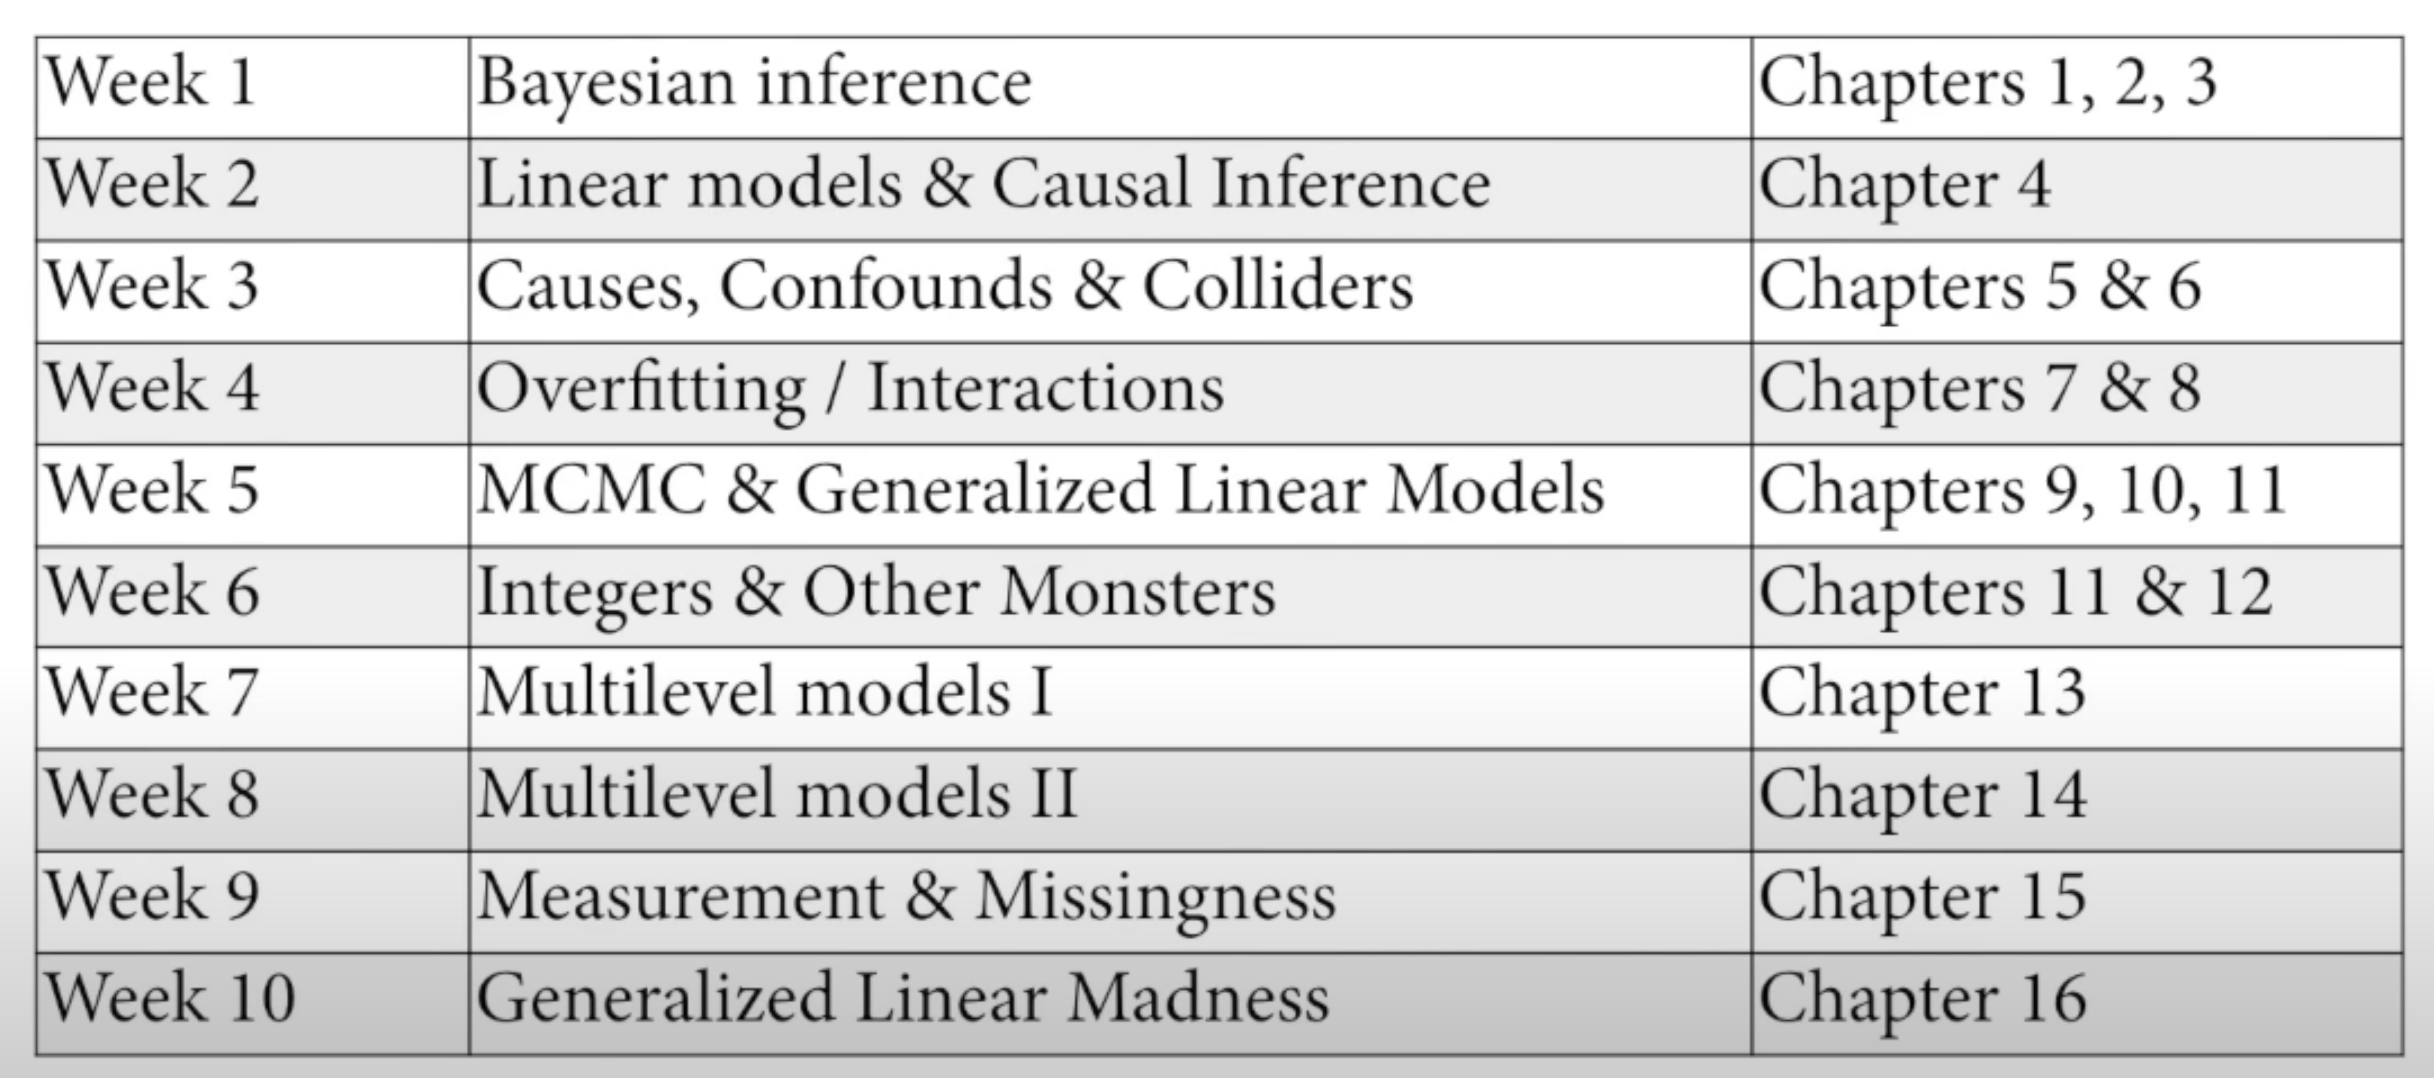
\includegraphics{img/SR2-Course-Schedule-min.png}

A better overview with links to videos and slides provides the following
HTML table, taken from the
\href{https://github.com/rmcelreath/stat_rethinking_2023/blob/main/README.md\#calendar--topical-outline}{README.md
file for the 2023 lectures}.

\begin{longtable}[]{@{}
  >{\raggedright\arraybackslash}p{(\columnwidth - 6\tabcolsep) * \real{0.0188}}
  >{\raggedright\arraybackslash}p{(\columnwidth - 6\tabcolsep) * \real{0.0264}}
  >{\raggedright\arraybackslash}p{(\columnwidth - 6\tabcolsep) * \real{0.0395}}
  >{\raggedright\arraybackslash}p{(\columnwidth - 6\tabcolsep) * \real{0.9153}}@{}}
\toprule\noalign{}
\begin{minipage}[b]{\linewidth}\raggedright
Week \#\#
\end{minipage} & \begin{minipage}[b]{\linewidth}\raggedright
Meeting date
\end{minipage} & \begin{minipage}[b]{\linewidth}\raggedright
Reading
\end{minipage} & \begin{minipage}[b]{\linewidth}\raggedright
Lectures
\end{minipage} \\
\midrule\noalign{}
\endhead
\bottomrule\noalign{}
\endlastfoot
Week 01 & 06 January & Chapters 1, 2 and 3 & {[}1{]}
\textless{}\href{https://www.youtube.com/watch?v=FdnMWdICdRs&list=PLDcUM9US4XdPz-KxHM4XHt7uUVGWWVSus&index=1}{Golem
of Prague}\textgreater{}
\textless{}\href{https://speakerdeck.com/rmcelreath/statistical-rethinking-2023-lecture-01}{Slides}\textgreater{}
{[}2{]}
\textless{}\href{https://www.youtube.com/watch?v=R1vcdhPBlXA&list=PLDcUM9US4XdPz-KxHM4XHt7uUVGWWVSus&index=2}{Garden
of Forking Data}\textgreater{}
\textless{}\href{https://speakerdeck.com/rmcelreath/statistical-rethinking-2023-lecture-02}{Slides}\textgreater{} \\
Week 02 & 13 January & Chapter 4 & {[}3{]}
\textless{}\href{https://www.youtube.com/watch?v=tNOu-SEacNU&list=PLDcUM9US4XdPz-KxHM4XHt7uUVGWWVSus&index=3}{Geocentric
Models}\textgreater{}
\textless{}\href{https://speakerdeck.com/rmcelreath/statistical-rethinking-2023-lecture-03}{Slides}\textgreater{}
{[}4{]}
\textless{}\href{https://www.youtube.com/watch?v=F0N4b7K_iYQ&list=PLDcUM9US4XdPz-KxHM4XHt7uUVGWWVSus&index=4}{Categories
and Curves}\textgreater{}
\textless{}\href{https://speakerdeck.com/rmcelreath/statistical-rethinking-2023-lecture-04}{Slides}\textgreater{} \\
Week 03 & 20 January & Chapters 5 and 6 & {[}5{]}
\textless{}\href{https://www.youtube.com/watch?v=mBEA7PKDmiY&list=PLDcUM9US4XdPz-KxHM4XHt7uUVGWWVSus&index=5}{Elemental
Confounds}\textgreater{}
\textless{}\href{https://speakerdeck.com/rmcelreath/statistical-rethinking-2023-lecture-05}{Slides}\textgreater{}
{[}6{]}
\textless{}\href{https://www.youtube.com/watch?v=uanZZLlzKHw&list=PLDcUM9US4XdPz-KxHM4XHt7uUVGWWVSus&index=6}{Good
and Bad Controls}\textgreater{}
\textless{}\href{https://speakerdeck.com/rmcelreath/statistical-rethinking-2023-lecture-06}{Slides}\textgreater{} \\
Week 04 & 27 January & Chapters 7,8,9 & {[}7{]}
\textless{}\href{https://www.youtube.com/watch?v=1VgYIsANQck&list=PLDcUM9US4XdPz-KxHM4XHt7uUVGWWVSus&index=7}{Overfitting}\textgreater{}
\textless{}\href{https://speakerdeck.com/rmcelreath/statistical-rethinking-2023-lecture-07}{Slides}\textgreater{}
{[}8{]}
\textless{}\href{https://www.youtube.com/watch?v=rZk2FqX2XnY&list=PLDcUM9US4XdPz-KxHM4XHt7uUVGWWVSus&index=8}{MCMC}\textgreater{}
\textless{}\href{https://speakerdeck.com/rmcelreath/statistical-rethinking-2023-lecture-08}{Slides}\textgreater{} \\
Week 05 & 03 February & Chapters 10 and 11 & {[}9{]}
\textless{}\href{https://www.youtube.com/watch?v=Zi6N3GLUJmw&list=PLDcUM9US4XdPz-KxHM4XHt7uUVGWWVSus&index=9}{Modeling
Events}\textgreater{}
\textless{}\href{https://speakerdeck.com/rmcelreath/statistical-rethinking-2023-lecture-09}{Slides}\textgreater{}
{[}10{]}
\textless{}\href{https://www.youtube.com/watch?v=jokxu18egu0&list=PLDcUM9US4XdPz-KxHM4XHt7uUVGWWVSus&index=10}{Counts
and Confounds}\textgreater{}
\textless{}\href{https://speakerdeck.com/rmcelreath/statistical-rethinking-2023-lecture-10}{Slides}\textgreater{} \\
Week 06 & 10 February & Chapters 11 and 12 & {[}11{]}
\textless{}\href{https://www.youtube.com/watch?v=VVQaIkom5D0&list=PLDcUM9US4XdPz-KxHM4XHt7uUVGWWVSus&index=11}{Ordered
Categories}\textgreater{}
\textless{}\href{https://github.com/rmcelreath/stat_rethinking_2023/raw/main/slides/Lecture_11-ord_logit.pdf}{Slides}\textgreater{}
{[}12{]}
\textless{}\href{https://www.youtube.com/watch?v=iwVqiiXYeC4&list=PLDcUM9US4XdPz-KxHM4XHt7uUVGWWVSus&index=12}{Multilevel
Models}\textgreater{}
\textless{}\href{https://raw.githubusercontent.com/rmcelreath/stat_rethinking_2023/main/slides/Lecture_12-GLMM1.pdf}{Slides}\textgreater{} \\
Week 07 & 17 February & Chapter 13 & {[}13{]}
\textless{}\href{https://www.youtube.com/watch?v=sgqMkZeslxA&list=PLDcUM9US4XdPz-KxHM4XHt7uUVGWWVSus&index=13}{Multilevel
Adventures}\textgreater{}
\textless{}\href{https://raw.githubusercontent.com/rmcelreath/stat_rethinking_2023/main/slides/Lecture_13-GLMM2.pdf}{Slides}\textgreater{}
{[}14{]}
\textless{}\href{https://www.youtube.com/watch?v=Es44-Bp1aKo&list=PLDcUM9US4XdPz-KxHM4XHt7uUVGWWVSus&index=14}{Correlated
Features}\textgreater{}
\textless{}\href{https://github.com/rmcelreath/stat_rethinking_2023/raw/main/slides/Lecture_14-GLMM3.pdf}{Slides}\textgreater{} \\
Week 08 & 24 February & Chapter 14 & {[}15{]}
\textless{}\href{https://www.youtube.com/watch?v=hnYhJzYAQ60&list=PLDcUM9US4XdPz-KxHM4XHt7uUVGWWVSus&index=15}{Social
Networks}\textgreater{}
\textless{}\href{https://github.com/rmcelreath/stat_rethinking_2023/raw/main/slides/Lecture_15-social_networks.pdf}{Slides}\textgreater{}
{[}16{]}
\textless{}\href{https://www.youtube.com/watch?v=Y2ZLt4iOrXU&list=PLDcUM9US4XdPz-KxHM4XHt7uUVGWWVSus&index=16}{Gaussian
Processes}\textgreater{}
\textless{}\href{https://github.com/rmcelreath/stat_rethinking_2023/raw/main/slides/Lecture_16-gaussian_processes.pdf}{Slides}\textgreater{} \\
Week 09 & 03 March & Chapter 15 & {[}17{]}
\textless{}\href{https://www.youtube.com/watch?v=mt9WKbQJrI4&list=PLDcUM9US4XdPz-KxHM4XHt7uUVGWWVSus&index=17}{Measurement}\textgreater{}
\textless{}\href{https://github.com/rmcelreath/stat_rethinking_2023/raw/main/slides/Lecture_17-measurement.pdf}{Slides}\textgreater{}
{[}18{]}
\textless{}\href{https://www.youtube.com/watch?v=Oeq6GChHOzc&list=PLDcUM9US4XdPz-KxHM4XHt7uUVGWWVSus&index=18}{Missing
Data}\textgreater{}
\textless{}\href{https://github.com/rmcelreath/stat_rethinking_2023/raw/main/slides/Lecture_18-missing_data.pdf}{Slides}\textgreater{} \\
Week 10 & 10 March & Chapters 16 and 17 & {[}19{]}
\textless{}\href{https://www.youtube.com/watch?v=zffwg0xDOgE&list=PLDcUM9US4XdPz-KxHM4XHt7uUVGWWVSus&index=19}{Generalized
Linear Madness}\textgreater{}
\textless{}\href{https://github.com/rmcelreath/stat_rethinking_2023/raw/main/slides/Lecture_19-GenLinearMadness.pdf}{Slides}\textgreater{}
{[}20{]}
\textless{}\href{https://www.youtube.com/watch?v=qwF-st2NGTU&list=PLDcUM9US4XdPz-KxHM4XHt7uUVGWWVSus&index=20&pp=sAQB}{Horoscopes}\textgreater{}
\textless{}\href{https://github.com/rmcelreath/stat_rethinking_2023/raw/main/slides/Lecture_20-horoscopes.pdf}{Slides}\textgreater{} \\
\end{longtable}

\hypertarget{important-links}{%
\section*{Important Links}\label{important-links}}
\addcontentsline{toc}{section}{Important Links}

\markright{Important Links}

\begin{itemize}
\tightlist
\item
  You can purchase \emph{Statistical Rethinking: A Bayesian Course in R
  and Stan} from
  \href{https://www.routledge.com/Statistical-Rethinking-A-Bayesian-Course-with-Examples-in-R-and-STAN/McElreath/p/book/9780367139919?utm_source=crcpress.com&utm_medium=referral}{CRC
  Press}.
\item
  \textbf{The \texttt{rethinking} package}: Statistical Rethinking
  course and book package:
  \url{https://github.com/rmcelreath/rethinking}. I am using version
  2.31.
\item
  \textbf{Statistical rethinking 2023}: Course material for January -
  March 2023. \url{https://github.com/rmcelreath/stat_rethinking_2023}.
  It contains a link to the new
  \href{https://www.youtube.com/watch?v=FdnMWdICdRs&list=PLDcUM9US4XdPz-KxHM4XHt7uUVGWWVSus}{Video
  playlist 2023}, and to the
  \href{https://speakerdeck.com/rmcelreath/}{slide deck collection}.
  Furthermore it displays a table with the readings per week including
  the links to the appropriate video and slides. The repo also inlcudes
  \href{https://github.com/petzi53/stat_rethinking_2023/tree/main/homework}{PDFs
  for the homework} and the
  \href{https://github.com/petzi53/stat_rethinking_2023/tree/main/homework}{scripts
  for the lecture animations}. --- I could not find the new R scripts
  associated with the (new) book text. They need to be collected from
  the slide lectures.
\item
  \textbf{Statistical rethinking with brms, ggplot2, and the tidyverse}:
  \href{https://bookdown.org/content/4857/}{brms/tidyverse-Conversion}
  of Statistical Rethinking using bookdown by \emph{A Solomon Kurz}
  (2023-01-26)
\item
  \textbf{Functions for Learning Bayesian Inference}: Maybe I should
  also check this resource: It is an
  \href{https://cran.r-project.org/package=LearnBayes}{R package to
  learn bayesian inference} with vignettes as short guides.
\end{itemize}

\textbf{Solutions}:

There are two different bookdown websites with book solutions:

\begin{itemize}
\tightlist
\item
  \href{https://bookdown.org/bgautijonsson/statistical_rethinking_solutions/}{Solutions
  for the 1st edition} by \emph{Brynjólfur Gauti Jónsson} and
\item
  \href{https://github.com/wjakethompson/sr2-solutions}{Solutions for
  the 2nd edition} by \emph{Jake Thompson.}
\end{itemize}

I have also found two GitHub repos with solutions:

\begin{itemize}
\tightlist
\item
  \href{https://github.com/jffist/statistical-rethinking-solutions}{GitHub
  solutions by \emph{Taras Svirskyi}} \emph{(jffist)}
\item
  \href{https://github.com/cavaunpeu/statistical-rethinking}{GitHub
  solutions by William Wolf} \emph{(cavaunpeu)}
\end{itemize}

\begin{tcolorbox}[enhanced jigsaw, colframe=quarto-callout-caution-color-frame, colback=white, toprule=.15mm, breakable, arc=.35mm, bottomtitle=1mm, colbacktitle=quarto-callout-caution-color!10!white, toptitle=1mm, titlerule=0mm, title=\textcolor{quarto-callout-caution-color}{\faFire}\hspace{0.5em}{Caution}, leftrule=.75mm, opacityback=0, rightrule=.15mm, opacitybacktitle=0.6, bottomrule=.15mm, left=2mm, coltitle=black]

These solutions are written by members of the \#RStats community and are
not authorized by the author.

\end{tcolorbox}

\bookmarksetup{startatroot}

\hypertarget{golem-of-prague}{%
\chapter{Golem of Prague}\label{golem-of-prague}}

A golem (goh-lem) is a clay robot from Jewish folklore. It stands as a
metaphor for scientific models. Like in the folklore they are made of
dust (silicon chips), are very powerful but also very dumb and therefore
dangerous.

There is nothing more in this chapter. I opened this file only to get
the same header numbers as in the book.

\bookmarksetup{startatroot}

\hypertarget{sec-small-and-large-worlds}{%
\chapter{Small and Large Worlds}\label{sec-small-and-large-worlds}}

\begin{Shaded}
\begin{Highlighting}[]
\InformationTok{\textasciigrave{}\textasciigrave{}\textasciigrave{}\{r\}}
\CommentTok{\#| label: setup}

\FunctionTok{library}\NormalTok{(tidyverse)}
\InformationTok{\textasciigrave{}\textasciigrave{}\textasciigrave{}}
\end{Highlighting}
\end{Shaded}

\begin{verbatim}
#> -- Attaching core tidyverse packages ------------------------ tidyverse 2.0.0 --
#> v dplyr     1.1.2     v readr     2.1.4
#> v forcats   1.0.0     v stringr   1.5.0
#> v ggplot2   3.4.2     v tibble    3.2.1
#> v lubridate 1.9.2     v tidyr     1.3.0
#> v purrr     1.0.1     
#> -- Conflicts ------------------------------------------ tidyverse_conflicts() --
#> x dplyr::filter() masks stats::filter()
#> x dplyr::lag()    masks stats::lag()
#> i Use the conflicted package (<http://conflicted.r-lib.org/>) to force all conflicts to become errors
\end{verbatim}

\begin{Shaded}
\begin{Highlighting}[]
\InformationTok{\textasciigrave{}\textasciigrave{}\textasciigrave{}\{r\}}
\CommentTok{\#| label: setup}

\FunctionTok{library}\NormalTok{(patchwork)}

\InformationTok{\textasciigrave{}\textasciigrave{}\textasciigrave{}}
\end{Highlighting}
\end{Shaded}

\begin{tcolorbox}[enhanced jigsaw, colframe=quarto-callout-note-color-frame, colback=white, toprule=.15mm, breakable, arc=.35mm, bottomtitle=1mm, colbacktitle=quarto-callout-note-color!10!white, toptitle=1mm, titlerule=0mm, title=\textcolor{quarto-callout-note-color}{\faInfo}\hspace{0.5em}{Setup chunk results in several output chunks}, leftrule=.75mm, opacityback=0, rightrule=.15mm, opacitybacktitle=0.6, bottomrule=.15mm, left=2mm, coltitle=black]

The single setup chunk produces in the output several separate chunks
that are tied with the specifics of the loaded packages. This split-up
helps to see the association of messages with their corresponding
packages.

\end{tcolorbox}

\hypertarget{original}{%
\section*{Original}\label{original}}
\addcontentsline{toc}{section}{Original}

\markright{Original}

\begin{itemize}
\tightlist
\item
  The \textbf{small world} is the self-contained logical world of the
  model.
\item
  The \textbf{large world} is the broader context in which one deploys a
  model.
\end{itemize}

\textbf{Meta Remark (Study Guide)}

\begin{quote}
This chapter focuses on the small world. It explains probability theory
in its essential form: counting the ways things can happen. Bayesian
inference arises automatically from this perspective. Then the chapter
presents the stylized components of a Bayesian statistical model, a
model for learning from data. Then it shows you how to animate the
model, to produce estimates.

All this work provides a foundation for the next chapter, in which
you'll learn to summarize Bayesian estimates, as well as begin to
consider large world obligations.
\end{quote}

\hypertarget{tidyverse}{%
\section*{Tidyverse}\label{tidyverse}}
\addcontentsline{toc}{section}{Tidyverse}

\markright{Tidyverse}

\textbf{Meta Remark (My Replication Strategy)}

The work by Solomon Kurz has many references to R specifics, so that
people new to R can follow the course. Most of these references are not
new to me, so I will not include them in my personal notes. There are
also very important references to other relevant articles I do not know.
But I will put these kind of references for now aside and will me mostly
concentrate on the replication and understanding of the code examples.

One challenge for the author (Kurz) was to replicate all the graphics of
the original version, even if they were produced just for understanding
without underlying code. I will use only code lines that are essential
to display Bayesian results. Therefore I will not replicate the very
extensive explication how to produce with tidyverse means the graphic of
the garden of forking data.

\hypertarget{the-garden-of-forking-data}{%
\section{The Garden of Forking Data}\label{the-garden-of-forking-data}}

\hypertarget{original-1}{%
\subsection{Original}\label{original-1}}

\begin{tcolorbox}[enhanced jigsaw, colframe=quarto-callout-tip-color-frame, colback=white, toprule=.15mm, breakable, arc=.35mm, bottomtitle=1mm, colbacktitle=quarto-callout-tip-color!10!white, toptitle=1mm, titlerule=0mm, title=\textcolor{quarto-callout-tip-color}{\faLightbulb}\hspace{0.5em}{Bayesian inference is counting of possibilities}, leftrule=.75mm, opacityback=0, rightrule=.15mm, opacitybacktitle=0.6, bottomrule=.15mm, left=2mm, coltitle=black]

Bayesian inference is really just counting and comparing of
possibilities. \ldots{} In order to make good inference about what
actually happened, it helps to consider everything that could have
happened. A Bayesian analysis is a garden of forking data, in which
alternative sequences of events are cultivated. As we learn about what
did happen, some of these alternative sequences are pruned. In the end,
what remains is only what is logically consistent with our knowledge.

\end{tcolorbox}

\hypertarget{counting-possibilities}{%
\subsubsection{Counting possibilities}\label{counting-possibilities}}

\begin{quote}
Suppose there's a bag, and it contains four marbles. These marbles come
in two colors: blue and white. We know there are four marbles in the
bag, but we don't know how many are of each color. We do know that there
are five possibilities: (1) {[}⚪⚪⚪⚪{]}, (2) {[}⚫⚪⚪⚪{]}, (3)
{[}⚫⚫⚪⚪{]}, (4) {[}⚫⚫⚫⚪{]}, (5) {[}⚫⚫⚫⚫{]}. These are the
only possibilities consistent with what we know about the contents of
the bag. \textbf{Call these five possibilities the \emph{conjectures}.}

Our goal is to figure out which of these conjectures is most plausible,
given some evidence about the contents of the bag. We do have some
evidence: A sequence of three marbles is pulled from the bag, one at a
time, replacing the marble each time and shaking the bag before drawing
another marble. \textbf{The sequence that emerges is: ⚫⚪⚫, in that
order. These are the data.} (bold emphasis pb)

So now let's plant the garden and see how to use the data to infer
what's in the bag. Let's begin by considering just the single
conjecture, {[}⚫⚪⚪⚪{]}, that the bag contains one blue and three
white marbles. \ldots{}

\ldots{}

Notice that even though the three white marbles look the same from a
data perspective---we just record the color of the marbles, after
all---they are really different events. This is important, because it
means that there are three more ways to see ⚪ than to see ⚫.
\end{quote}

\begin{longtable}[]{@{}ll@{}}
\toprule\noalign{}
\endhead
\bottomrule\noalign{}
\endlastfoot
Conjecture & Ways to produce ⚫⚪⚫ \\
{[}⚪⚪⚪⚪{]} & 0 × 4 × 0 = 0 \\
{[}⚫⚪⚪⚪{]} & 1 × 3 × 1 = 3 \\
{[}⚫⚫⚪⚪{]} & 2 × 2 × 2 = 8 \\
{[}⚫⚫⚫⚪{]} & 3 × 1 × 3 = 9 \\
{[}⚫⚫⚫⚫{]} & 4 × 0 × 4 = 0 \\
\end{longtable}

I have bypassed the counting procedure related with the step-by-step
visualization of the garden of forking data. The multiplication in the
above table is still a summarized counting:

\begin{tcolorbox}[enhanced jigsaw, colframe=quarto-callout-important-color-frame, colback=white, toprule=.15mm, breakable, arc=.35mm, bottomtitle=1mm, colbacktitle=quarto-callout-important-color!10!white, toptitle=1mm, titlerule=0mm, title=\textcolor{quarto-callout-important-color}{\faExclamation}\hspace{0.5em}{Important}, leftrule=.75mm, opacityback=0, rightrule=.15mm, opacitybacktitle=0.6, bottomrule=.15mm, left=2mm, coltitle=black]

\begin{quote}
Multiplication is just a shortcut to enumerating and counting up all of
the paths through the garden that could produce all the observations.
\end{quote}

\end{tcolorbox}

\begin{quote}
Notice that the number of ways to produce the data, for each conjecture,
can be computed by first counting the number of paths in each ``ring''
of the garden and then by multiplying these counts together. \ldots{}
The fact that numbers are multiplied during calculation doesn't change
the fact that this is still just counting of logically possible paths.
This point will come up again, when you meet a formal representation of
Bayesian inference.
\end{quote}

The multiplication in the above table has to be interpreted the
following way:

\begin{enumerate}
\def\labelenumi{\arabic{enumi}.}
\tightlist
\item
  The possibility of the conjecture that the bag contains four white
  marbles is zero because the result shows also black marbles. This is
  the other way around for the last conjecture of four blue/black
  marbles.
\item
  The possibility of the conjecture that the bag contains one black and
  three white marbles is calculated the following way: The first marble
  of the result is black and --- according to our conjecture --- there
  is only one way (=1) to produce this black marble. The next marble we
  have drawn is white. This is consistent with three (=3) different
  ways( marbles) of our conjecture. The last drawn marble is again black
  which corresponds again with just one way (possibility) following our
  conjecture. So we get as result of the garden of forking data:
  \texttt{1\ x\ 3\ x\ 1}.
\item
  The calculation of the other conjectures follows the same pattern.
\end{enumerate}

\hypertarget{combining-other-information}{%
\subsubsection{Combining Other
Information}\label{combining-other-information}}

\begin{quote}
We may have additional information about the relative plausibility of
each conjecture. This information could arise from knowledge of how the
contents of the bag were generated. It could also arise from previous
data. Whatever the source, it would help to have a way to combine
different sources of information to update the plausibilities. Luckily
there is a natural solution: Just multiply the counts.

To grasp this solution, suppose we're willing to say each conjecture is
equally plausible at the start. So we just compare the counts of ways in
which each conjecture is compatible with the observed data. This
comparison suggests that {[}⚫⚫⚫⚪{]} is slightly more plausible than
{[}⚫⚫⚪⚪{]}, and both are about three times more plausible than
{[}⚫⚪⚪⚪{]}. \textbf{Since these are our initial counts, and we are
going to update them next, let's label them \emph{prior}.} (bold
emphasis pb)
\end{quote}

\begin{tcolorbox}[enhanced jigsaw, colframe=quarto-callout-tip-color-frame, colback=white, toprule=.15mm, breakable, arc=.35mm, bottomtitle=1mm, colbacktitle=quarto-callout-tip-color!10!white, toptitle=1mm, titlerule=0mm, title=\textcolor{quarto-callout-tip-color}{\faLightbulb}\hspace{0.5em}{Principle of Indifference}, leftrule=.75mm, opacityback=0, rightrule=.15mm, opacitybacktitle=0.6, bottomrule=.15mm, left=2mm, coltitle=black]

As we will see later: the choice of the prior is not relevant for the
final result. This is called the \emph{Principle of Indifference}.

The only difference between a good or bad choice is the time (the number
of steps) the updating process needs to produce the final result.

Before seeing any data the most common solution is to assign an equal
number of ways that each conjecture could be correct.

\end{tcolorbox}

\begin{quote}
Which assumption should we use, when there is no previous information
about the conjectures? The most common solution is to assign an equal
number of ways that each conjecture could be correct, before seeing any
data. This is sometimes known as the \textbf{PRINCIPLE OF INDIFFERENCE}:
When there is no reason to say that one conjecture is more plausible
than another, weigh all of the conjectures equally. \ldots{}

For the sort of problems we examine in this book, the principle of
indifference results in inferences very comparable to mainstream
non-Bayesian approaches, most of which contain implicit equal weighting
of possibilities. For example a typical non-Bayesian confidence interval
weighs equally all of the possible values a parameter could take,
regardless of how implausible some of them are. In addition, many
non-Bayesian procedures have moved away from equal weighting, through
the use of penalized likelihood and other methods.
\end{quote}

\textbf{Bayesian Updating Process}

Here's how we do the updating:

\begin{enumerate}
\def\labelenumi{\arabic{enumi}.}
\tightlist
\item
  First we count the numbers of ways each conjecture could produce the
  new observation, ⚫.
\item
  Then we multiply each of these new counts by the prior numbers of ways
  for each conjecture.
\end{enumerate}

\begin{longtable}[]{@{}
  >{\raggedright\arraybackslash}p{(\columnwidth - 16\tabcolsep) * \real{0.1111}}
  >{\raggedright\arraybackslash}p{(\columnwidth - 16\tabcolsep) * \real{0.1111}}
  >{\raggedright\arraybackslash}p{(\columnwidth - 16\tabcolsep) * \real{0.1111}}
  >{\raggedright\arraybackslash}p{(\columnwidth - 16\tabcolsep) * \real{0.1111}}
  >{\raggedright\arraybackslash}p{(\columnwidth - 16\tabcolsep) * \real{0.1111}}
  >{\raggedright\arraybackslash}p{(\columnwidth - 16\tabcolsep) * \real{0.1111}}
  >{\raggedright\arraybackslash}p{(\columnwidth - 16\tabcolsep) * \real{0.1111}}
  >{\raggedright\arraybackslash}p{(\columnwidth - 16\tabcolsep) * \real{0.1111}}
  >{\raggedright\arraybackslash}p{(\columnwidth - 16\tabcolsep) * \real{0.1111}}@{}}
\toprule\noalign{}
\endhead
\bottomrule\noalign{}
\endlastfoot
& & & & & & & & \\
& Conjecture & & Ways to produce ⚫ & & Prior counts & & New count & \\
& {[}⚪⚪⚪⚪{]} & & 0 & & 0 & & 0 × 0 = 0 & \\
& {[}⚫⚪⚪⚪{]} & & 1 & & 3 & & 3 × 1 = 3 & \\
& {[}⚫⚫⚪⚪{]} & & 2 & & 8 & & 8 × 2 = 16 & \\
& {[}⚫⚫⚫⚪{]} & & 3 & & 9 & & 9 × 3 = 27 & \\
& {[}⚫⚫⚫⚫{]} & & 4 & & 0 & & 0 × 4 = 0 & \\
\end{longtable}

\begin{tcolorbox}[enhanced jigsaw, colframe=quarto-callout-note-color-frame, colback=white, toprule=.15mm, breakable, arc=.35mm, bottomtitle=1mm, colbacktitle=quarto-callout-note-color!10!white, toptitle=1mm, titlerule=0mm, title=\textcolor{quarto-callout-note-color}{\faInfo}\hspace{0.5em}{Typo}, leftrule=.75mm, opacityback=0, rightrule=.15mm, opacitybacktitle=0.6, bottomrule=.15mm, left=2mm, coltitle=black]

In the book the table header ``Ways to produce'' includes ⚪ instead of
--- as I think is correct --- ⚫.

\end{tcolorbox}

\hypertarget{from-counts-to-probability}{%
\subsubsection{From Counts to
Probability}\label{from-counts-to-probability}}

\begin{tcolorbox}[enhanced jigsaw, colframe=quarto-callout-tip-color-frame, colback=white, toprule=.15mm, breakable, arc=.35mm, bottomtitle=1mm, colbacktitle=quarto-callout-tip-color!10!white, toptitle=1mm, titlerule=0mm, title=\textcolor{quarto-callout-tip-color}{\faLightbulb}\hspace{0.5em}{Principle of honest ignorance}, leftrule=.75mm, opacityback=0, rightrule=.15mm, opacitybacktitle=0.6, bottomrule=.15mm, left=2mm, coltitle=black]

\emph{When we don't know what caused the data, potential causes that may
produce the data in more ways are more plausible}.

\end{tcolorbox}

Two reasons for using probabilities instead of counts:

\begin{enumerate}
\def\labelenumi{\arabic{enumi}.}
\tightlist
\item
  Only relative value matters.
\item
  Counts will very fast grow very large and difficult to manipulate.
\end{enumerate}

\begin{figure}

{\centering 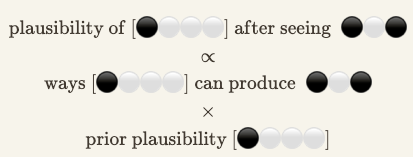
\includegraphics{img/plausibility-formula-1-min.png}

}

\end{figure}

\textbf{Standardizing the plausibility}

\begin{figure}

{\centering 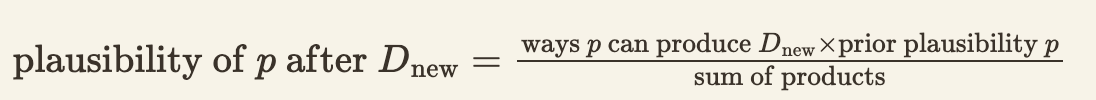
\includegraphics{img/plausibility-formula-2-min.png}

}

\end{figure}

\begin{Shaded}
\begin{Highlighting}[]
\InformationTok{\textasciigrave{}\textasciigrave{}\textasciigrave{}\{r\}}
\CommentTok{\#| label: compute{-}plausibilities}

\DocumentationTok{\#\# R code 2.1}
\NormalTok{ways }\OtherTok{\textless{}{-}} \FunctionTok{c}\NormalTok{(}\DecValTok{0}\NormalTok{, }\DecValTok{3}\NormalTok{, }\DecValTok{8}\NormalTok{, }\DecValTok{9}\NormalTok{, }\DecValTok{0}\NormalTok{)}
\NormalTok{ways }\SpecialCharTok{/} \FunctionTok{sum}\NormalTok{(ways)}
\InformationTok{\textasciigrave{}\textasciigrave{}\textasciigrave{}}
\end{Highlighting}
\end{Shaded}

\begin{verbatim}
#> [1] 0.00 0.15 0.40 0.45 0.00
\end{verbatim}

I understand that in the above code we assume as the very first prior
plausibility the ways the results can be produced by the assumed
conjecture proportion of blue marbles. It corresponds to the parameter
value. This conclusion is somewhat hidden as our very first calculation
already takes three drawn marbles (⚫⚪⚫) into account. From another
perspective this could also be seen as the first draw (⚫) followed by
two Bayesian updates (⚪⚫). This corresponds to the following counting:
(In the second and third draw the first factor of the multiplication is
always the prior.)

\begin{enumerate}
\def\labelenumi{\arabic{enumi}.}
\tightlist
\item
  First draw ⚫: 0,1,2,3,4 ways corresponding to the 4 chosen
  conjectures.
\item
  Second draw ⚪: 0 x 4 = 0, 1 x 3 = 3, 2 x 2 = 4, 3 x 1 = 3, 4 x 0 = 0
\item
  Third draw ⚫: 0 x 0 = 0, 3 x 1 = 3, 4 x 2 = 8, 3 x 3 = 9, 0 x 4 = 0
\end{enumerate}

This demonstration shows that the book example of ⚫⚪⚫ already
contains three priors: The first is identical with the conjectured
proportion of blue marbles (0,1,2,3,4) and is equivalent to the
parameter value for each conjecture. The second and third marbles
already uses Bayesian updating.

\textbf{Names of the different parts of the formula}

Data = ⚫⚪⚫.

\begin{itemize}
\tightlist
\item
  A conjectured proportion of blue marbles, \emph{p}, is usually called
  a \textbf{PARAMETER} value. It's just a way of indexing possible
  explanations of the data. For instance one conjectured proportion of
  one blue marble could be: ⚫⚪⚪⚪ (\texttt{p\ =\ 1}). The others are:
  ⚪⚪⚪⚪ (\texttt{p\ =\ 0}), ⚫⚫⚪⚪ (\texttt{p\ =\ 2} , ⚫⚫⚫⚪
  (\texttt{p\ =\ 3}), and ⚫⚫⚫⚫ (\texttt{p\ =\ 4} ways).
\item
  The relative number of ways that a value \emph{p} can produce the data
  is usually called a \textbf{LIKELIHOOD}. It is derived by enumerating
  all the possible data sequences that could have happened and then
  eliminating those sequences inconsistent with the data. For instance:
  \texttt{0.00,\ 0.15,\ 0.40,\ 0.45,\ 0.00}
\item
  The prior plausibility of any specific \emph{p} is usually called the
  \textbf{PRIOR PROBABILITY}. For instance: \texttt{0,\ 3,\ 8,\ 9,\ 0}
\item
  The new, updated plausibility of any specific \emph{p} is usually
  called the \textbf{POSTERIOR PROBABILITY}. For instance:
  \texttt{0,\ 3,\ 16,\ 27,\ 0}
\end{itemize}

\hypertarget{tidyverse-1}{%
\subsection{Tidyverse}\label{tidyverse-1}}

\hypertarget{counting-possibilities-1}{%
\subsubsection{Counting possibilities}\label{counting-possibilities-1}}

\begin{quote}
If we're willing to code the marbles as 0 = ``white'' 1 = ``blue'', we
can arrange the possibility data in a tibble as follows.
\end{quote}

\begin{tcolorbox}[enhanced jigsaw, colframe=quarto-callout-note-color-frame, colback=white, toprule=.15mm, breakable, arc=.35mm, bottomtitle=1mm, colbacktitle=quarto-callout-note-color!10!white, toptitle=1mm, titlerule=0mm, title=\textcolor{quarto-callout-note-color}{\faInfo}\hspace{0.5em}{Changed code slightly}, leftrule=.75mm, opacityback=0, rightrule=.15mm, opacitybacktitle=0.6, bottomrule=.15mm, left=2mm, coltitle=black]

I changed \texttt{rep()} to \texttt{rep.int()} and added \texttt{L} to
the value of p1 resp. p5 to get integers (instead of doubles).

\end{tcolorbox}

\begin{Shaded}
\begin{Highlighting}[]
\InformationTok{\textasciigrave{}\textasciigrave{}\textasciigrave{}\{r\}}
\CommentTok{\#| label: create{-}marble{-}data}

\NormalTok{d }\OtherTok{\textless{}{-}}
\NormalTok{  tibble}\SpecialCharTok{::}\FunctionTok{tibble}\NormalTok{(}\AttributeTok{p1 =}\NormalTok{ 0L,}
         \AttributeTok{p2 =} \FunctionTok{rep.int}\NormalTok{(}\DecValTok{1}\SpecialCharTok{:}\DecValTok{0}\NormalTok{, }\AttributeTok{times =} \FunctionTok{c}\NormalTok{(}\DecValTok{1}\NormalTok{, }\DecValTok{3}\NormalTok{)),}
         \AttributeTok{p3 =} \FunctionTok{rep.int}\NormalTok{(}\DecValTok{1}\SpecialCharTok{:}\DecValTok{0}\NormalTok{, }\AttributeTok{times =} \FunctionTok{c}\NormalTok{(}\DecValTok{2}\NormalTok{, }\DecValTok{2}\NormalTok{)),}
         \AttributeTok{p4 =} \FunctionTok{rep.int}\NormalTok{(}\DecValTok{1}\SpecialCharTok{:}\DecValTok{0}\NormalTok{, }\AttributeTok{times =} \FunctionTok{c}\NormalTok{(}\DecValTok{3}\NormalTok{, }\DecValTok{1}\NormalTok{)),}
         \AttributeTok{p5 =}\NormalTok{ 1L)}

\FunctionTok{head}\NormalTok{(d)}
\InformationTok{\textasciigrave{}\textasciigrave{}\textasciigrave{}}
\end{Highlighting}
\end{Shaded}

\begin{verbatim}
#> # A tibble: 4 x 5
#>      p1    p2    p3    p4    p5
#>   <int> <int> <int> <int> <int>
#> 1     0     1     1     1     1
#> 2     0     0     1     1     1
#> 3     0     0     0     1     1
#> 4     0     0     0     0     1
\end{verbatim}

\begin{quote}
You might depict the possibility data in a plot.
\end{quote}

\begin{codelisting}[H]

\caption{Code listing to show the marble data as graph}

\hypertarget{lst-marble-data}{%
\label{lst-marble-data}}%
\begin{Shaded}
\begin{Highlighting}[]
\InformationTok{\textasciigrave{}\textasciigrave{}\textasciigrave{}\{r\}}
\CommentTok{\#| label: fig{-}show{-}marble{-}data}
\CommentTok{\#| fig{-}cap: "Marble Data"}
\CommentTok{\#| attr{-}source: \textquotesingle{}\#lst{-}marble{-}data lst{-}cap="Code listing to show the marble data as graph"\textquotesingle{}}


\NormalTok{d }\SpecialCharTok{\%\textgreater{}\%} 
  \FunctionTok{set\_names}\NormalTok{(}\DecValTok{1}\SpecialCharTok{:}\DecValTok{5}\NormalTok{) }\SpecialCharTok{\%\textgreater{}\%}    \hspace*{\fill}\NormalTok{\circled{1}}
  \FunctionTok{mutate}\NormalTok{(}\AttributeTok{x =} \DecValTok{1}\SpecialCharTok{:}\DecValTok{4}\NormalTok{) }\SpecialCharTok{\%\textgreater{}\%}  \hspace*{\fill}\NormalTok{\circled{2}}
  \FunctionTok{pivot\_longer}\NormalTok{(}\SpecialCharTok{{-}}\NormalTok{x, }\AttributeTok{names\_to =} \StringTok{"possibility"}\NormalTok{) }\SpecialCharTok{\%\textgreater{}\%}  \hspace*{\fill}\NormalTok{\circled{3}}
  \FunctionTok{mutate}\NormalTok{(}\AttributeTok{value =}\NormalTok{ value }\SpecialCharTok{\%\textgreater{}\%} \FunctionTok{as.character}\NormalTok{()) }\SpecialCharTok{\%\textgreater{}\%}    \hspace*{\fill}\NormalTok{\circled{4}}
  
  \FunctionTok{ggplot}\NormalTok{(}\FunctionTok{aes}\NormalTok{(}\AttributeTok{x =}\NormalTok{ x, }\AttributeTok{y =}\NormalTok{ possibility, }\AttributeTok{fill =}\NormalTok{ value)) }\SpecialCharTok{+} \hspace*{\fill}\NormalTok{\circled{5}}
  \FunctionTok{geom\_point}\NormalTok{(}\AttributeTok{shape =} \DecValTok{21}\NormalTok{, }\AttributeTok{size =} \DecValTok{5}\NormalTok{) }\SpecialCharTok{+} 
  \FunctionTok{scale\_fill\_manual}\NormalTok{(}\AttributeTok{values =} \FunctionTok{c}\NormalTok{(}\StringTok{"white"}\NormalTok{, }\StringTok{"navy"}\NormalTok{)) }\SpecialCharTok{+} 
  \FunctionTok{scale\_x\_discrete}\NormalTok{(}\ConstantTok{NULL}\NormalTok{, }\AttributeTok{breaks =} \ConstantTok{NULL}\NormalTok{) }\SpecialCharTok{+} 
  \FunctionTok{theme}\NormalTok{(}\AttributeTok{legend.position =} \StringTok{"none"}\NormalTok{) }
 
\InformationTok{\textasciigrave{}\textasciigrave{}\textasciigrave{}}
\end{Highlighting}
\end{Shaded}

\end{codelisting}

\begin{description}
\tightlist
\item[\circled{1}]
Change the column names from p\textless number\textgreater{} to
\textless number\textgreater.
\item[\circled{2}]
Add a new column with the values 1 to 4 for each row.
\item[\circled{3}]
Convert data frame from wide to long, excluding the \texttt{x} column.
\item[\circled{4}]
Change the variable type of \texttt{value} column from double to
character.
\item[\circled{5}]
Plot the results.
\end{description}

\begin{figure}[H]

{\centering 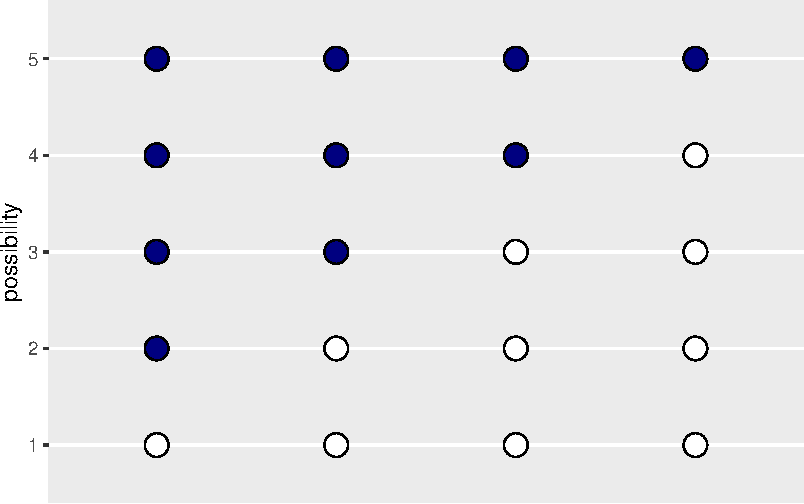
\includegraphics{02-small-and-large-worlds_files/figure-pdf/fig-show-marble-data-1.pdf}

}

\caption{\label{fig-show-marble-data}Marble Data}

\end{figure}

At first I could not understand the code lines. I had to execute line by
line to see what happens:

\hypertarget{annotation-1}{%
\paragraph{Annotation (1)}\label{annotation-1}}

\begin{Shaded}
\begin{Highlighting}[]
\InformationTok{\textasciigrave{}\textasciigrave{}\textasciigrave{}\{r\}}
\CommentTok{\#| label: using{-}set{-}names}

\FunctionTok{set\_names}\NormalTok{(d, }\DecValTok{1}\SpecialCharTok{:}\DecValTok{5}\NormalTok{)}
\InformationTok{\textasciigrave{}\textasciigrave{}\textasciigrave{}}
\end{Highlighting}
\end{Shaded}

\begin{verbatim}
#> # A tibble: 4 x 5
#>     `1`   `2`   `3`   `4`   `5`
#>   <int> <int> <int> <int> <int>
#> 1     0     1     1     1     1
#> 2     0     0     1     1     1
#> 3     0     0     0     1     1
#> 4     0     0     0     0     1
\end{verbatim}

\texttt{rlang::set\_names()} comes from \{\textbf{rlang}\} package which
contains function for base types and core tidyverse features. It is
exported to \{\textbf{purrr}\}, a package with tools for functional
programming. It is equivalent to \texttt{stats::setNames()} but has more
features and stricter argument checking. I does nothing more as to
change the column names from p\textless number\textgreater{} to
\textless number\textgreater. If one had used just numbers for the
probability columns this line wouldn't have been necessary as it is
shown in the next chunk. (I omitted the \texttt{utils::head()} argument
of the last line as it is not necessary.)

\begin{Shaded}
\begin{Highlighting}[]
\InformationTok{\textasciigrave{}\textasciigrave{}\textasciigrave{}\{r\}}
\CommentTok{\#| label: create{-}marble{-}data{-}2}

\NormalTok{df }\OtherTok{\textless{}{-}}
  \FunctionTok{tibble}\NormalTok{(}\StringTok{\textasciigrave{}}\AttributeTok{1}\StringTok{\textasciigrave{}} \OtherTok{=} \DecValTok{0}\NormalTok{,}
         \StringTok{\textasciigrave{}}\AttributeTok{2}\StringTok{\textasciigrave{}} \OtherTok{=} \FunctionTok{rep}\NormalTok{(}\DecValTok{1}\SpecialCharTok{:}\DecValTok{0}\NormalTok{, }\AttributeTok{times =} \FunctionTok{c}\NormalTok{(}\DecValTok{1}\NormalTok{, }\DecValTok{3}\NormalTok{)),}
         \StringTok{\textasciigrave{}}\AttributeTok{3}\StringTok{\textasciigrave{}} \OtherTok{=} \FunctionTok{rep}\NormalTok{(}\DecValTok{1}\SpecialCharTok{:}\DecValTok{0}\NormalTok{, }\AttributeTok{times =} \FunctionTok{c}\NormalTok{(}\DecValTok{2}\NormalTok{, }\DecValTok{2}\NormalTok{)),}
         \StringTok{\textasciigrave{}}\AttributeTok{4}\StringTok{\textasciigrave{}} \OtherTok{=} \FunctionTok{rep}\NormalTok{(}\DecValTok{1}\SpecialCharTok{:}\DecValTok{0}\NormalTok{, }\AttributeTok{times =} \FunctionTok{c}\NormalTok{(}\DecValTok{3}\NormalTok{, }\DecValTok{1}\NormalTok{)),}
         \StringTok{\textasciigrave{}}\AttributeTok{5}\StringTok{\textasciigrave{}} \OtherTok{=} \DecValTok{1}\NormalTok{)}

\NormalTok{df}
\InformationTok{\textasciigrave{}\textasciigrave{}\textasciigrave{}}
\end{Highlighting}
\end{Shaded}

\begin{verbatim}
#> # A tibble: 4 x 5
#>     `1`   `2`   `3`   `4`   `5`
#>   <dbl> <int> <int> <int> <dbl>
#> 1     0     1     1     1     1
#> 2     0     0     1     1     1
#> 3     0     0     0     1     1
#> 4     0     0     0     0     1
\end{verbatim}

It is interesting to see that the first and last column are doubles and
not integers. I believe that the reason is that these two columns do not
have variations, e.g.~do not contain both variable values, so that R
assumes the more general class of \texttt{numeric} and type of
\texttt{double}.

\begin{itemize}
\tightlist
\item
  \texttt{class(5L)} and \texttt{typeof(5L}) both results to
  \emph{integer} .
\item
  Whereas \texttt{class(5)} is \emph{integer} but \texttt{typeof(5)} is
  \emph{double}.
\end{itemize}

\begin{Shaded}
\begin{Highlighting}[]
\InformationTok{\textasciigrave{}\textasciigrave{}\textasciigrave{}\{r\}}
\CommentTok{\#| label: number{-}types}

\FunctionTok{class}\NormalTok{(5L)}
\FunctionTok{typeof}\NormalTok{(5L)}
\FunctionTok{class}\NormalTok{(}\DecValTok{5}\NormalTok{)}
\FunctionTok{typeof}\NormalTok{(}\DecValTok{5}\NormalTok{)}
\InformationTok{\textasciigrave{}\textasciigrave{}\textasciigrave{}}
\end{Highlighting}
\end{Shaded}

\begin{verbatim}
#> [1] "integer"
#> [1] "integer"
#> [1] "numeric"
#> [1] "double"
\end{verbatim}

\hypertarget{annotation-2}{%
\paragraph{Annotation (2)}\label{annotation-2}}

After understanding what \texttt{stats::set\_names()} does the next line
with \texttt{dplyr::mutate()} is easy. It adds a new column \texttt{x}
with the values 1 to 4 for each row.

\begin{Shaded}
\begin{Highlighting}[]
\InformationTok{\textasciigrave{}\textasciigrave{}\textasciigrave{}\{r\}}
\CommentTok{\#| label: add{-}x{-}column}

\NormalTok{df }\OtherTok{\textless{}{-}}\NormalTok{ df }\SpecialCharTok{|\textgreater{}} 
    \FunctionTok{set\_names}\NormalTok{(}\DecValTok{1}\SpecialCharTok{:}\DecValTok{5}\NormalTok{) }\SpecialCharTok{|\textgreater{}} 
    \FunctionTok{mutate}\NormalTok{(}\AttributeTok{x =} \DecValTok{1}\SpecialCharTok{:}\DecValTok{4}\NormalTok{)}
\NormalTok{df}
\InformationTok{\textasciigrave{}\textasciigrave{}\textasciigrave{}}
\end{Highlighting}
\end{Shaded}

\begin{verbatim}
#> # A tibble: 4 x 6
#>     `1`   `2`   `3`   `4`   `5`     x
#>   <dbl> <int> <int> <int> <dbl> <int>
#> 1     0     1     1     1     1     1
#> 2     0     0     1     1     1     2
#> 3     0     0     0     1     1     3
#> 4     0     0     0     0     1     4
\end{verbatim}

\hypertarget{annotation-3}{%
\paragraph{Annotation (3)}\label{annotation-3}}

I understood that the data frame is converted from a wide to a long
structure. But together with the pipe and not naming the first parameter
\texttt{-x} I did not catch the essence of the command.

A first understanding comes from the fact, that it is wrong to covert
all columns to the long format:

\begin{Shaded}
\begin{Highlighting}[]
\InformationTok{\textasciigrave{}\textasciigrave{}\textasciigrave{}\{r\}}
\CommentTok{\#| label: wrong{-}long{-}conversion}

\FunctionTok{pivot\_longer}\NormalTok{(}\AttributeTok{data =}\NormalTok{ df, }\AttributeTok{cols =} \FunctionTok{everything}\NormalTok{(), }\AttributeTok{names\_to =} \StringTok{"possibility"}\NormalTok{) }\SpecialCharTok{|\textgreater{}} 
    \FunctionTok{print}\NormalTok{(}\AttributeTok{n =} \DecValTok{24}\NormalTok{)}
\InformationTok{\textasciigrave{}\textasciigrave{}\textasciigrave{}}
\end{Highlighting}
\end{Shaded}

\begin{verbatim}
#> # A tibble: 24 x 2
#>    possibility value
#>    <chr>       <dbl>
#>  1 1               0
#>  2 2               1
#>  3 3               1
#>  4 4               1
#>  5 5               1
#>  6 x               1
#>  7 1               0
#>  8 2               0
#>  9 3               1
#> 10 4               1
#> 11 5               1
#> 12 x               2
#> 13 1               0
#> 14 2               0
#> 15 3               0
#> 16 4               1
#> 17 5               1
#> 18 x               3
#> 19 1               0
#> 20 2               0
#> 21 3               0
#> 22 4               0
#> 23 5               1
#> 24 x               4
\end{verbatim}

This (wrong) example shows that it is mandatory to exclude \texttt{x}
from the conversion. Otherwise it would be included and integrated into
the \texttt{possibility} column.

\begin{Shaded}
\begin{Highlighting}[]
\InformationTok{\textasciigrave{}\textasciigrave{}\textasciigrave{}\{r\}}
\CommentTok{\#| label: correct{-}long{-}conversion}

\NormalTok{(d }\OtherTok{\textless{}{-}} 
    \FunctionTok{pivot\_longer}\NormalTok{(}\AttributeTok{data =}\NormalTok{ df, }\AttributeTok{cols =} \SpecialCharTok{{-}}\NormalTok{x, }\AttributeTok{names\_to =} \StringTok{"possibility"}\NormalTok{))}
\InformationTok{\textasciigrave{}\textasciigrave{}\textasciigrave{}}
\end{Highlighting}
\end{Shaded}

\begin{verbatim}
#> # A tibble: 20 x 3
#>        x possibility value
#>    <int> <chr>       <dbl>
#>  1     1 1               0
#>  2     1 2               1
#>  3     1 3               1
#>  4     1 4               1
#>  5     1 5               1
#>  6     2 1               0
#>  7     2 2               0
#>  8     2 3               1
#>  9     2 4               1
#> 10     2 5               1
#> 11     3 1               0
#> 12     3 2               0
#> 13     3 3               0
#> 14     3 4               1
#> 15     3 5               1
#> 16     4 1               0
#> 17     4 2               0
#> 18     4 3               0
#> 19     4 4               0
#> 20     4 5               1
\end{verbatim}

The above code line for the conversion from wide to long is equivalent
with naming explicitly all column names to convert:

\begin{Shaded}
\begin{Highlighting}[]
\InformationTok{\textasciigrave{}\textasciigrave{}\textasciigrave{}\{r\}}
\CommentTok{\#| label: test{-}if{-}identical}

\NormalTok{d1 }\OtherTok{\textless{}{-}} \FunctionTok{pivot\_longer}\NormalTok{(}\AttributeTok{data =}\NormalTok{ df, }\AttributeTok{cols =} \SpecialCharTok{{-}}\NormalTok{x, }\AttributeTok{names\_to =} \StringTok{"possibility"}\NormalTok{)}
\NormalTok{d2 }\OtherTok{\textless{}{-}} \FunctionTok{pivot\_longer}\NormalTok{(}\AttributeTok{data =}\NormalTok{ df, }
                   \AttributeTok{cols =} \FunctionTok{c}\NormalTok{(}\StringTok{\textasciigrave{}}\AttributeTok{1}\StringTok{\textasciigrave{}}\NormalTok{, }\StringTok{\textasciigrave{}}\AttributeTok{2}\StringTok{\textasciigrave{}}\NormalTok{, }\StringTok{\textasciigrave{}}\AttributeTok{3}\StringTok{\textasciigrave{}}\NormalTok{, }\StringTok{\textasciigrave{}}\AttributeTok{4}\StringTok{\textasciigrave{}}\NormalTok{, }\StringTok{\textasciigrave{}}\AttributeTok{5}\StringTok{\textasciigrave{}}\NormalTok{), }
                   \AttributeTok{names\_to =} \StringTok{"possibility"}\NormalTok{)}
\FunctionTok{identical}\NormalTok{(d1, d2)}
\InformationTok{\textasciigrave{}\textasciigrave{}\textasciigrave{}}
\end{Highlighting}
\end{Shaded}

\begin{verbatim}
#> [1] TRUE
\end{verbatim}

The identity demonstrates: The \texttt{-x} parameter excludes the
\texttt{x} column from the wide to long transformation. It is a
shorthand for naming all 5 columns that should be transformed.

Instead of the \texttt{base::identical()} function you could also use
\texttt{base::all.equal()}. Comparing data frames is a rather
complicated action summarized by a blog post from Sharla Gelfand. But
keep in mind that the publication date is 2020-02-17 and that therefore
some commands are outdated. Most important: use
\texttt{base::all.equal()} instead of \texttt{dplyr::all\_equal()}.

\begin{tcolorbox}[enhanced jigsaw, colframe=quarto-callout-warning-color-frame, colback=white, toprule=.15mm, breakable, arc=.35mm, bottomtitle=1mm, colbacktitle=quarto-callout-warning-color!10!white, toptitle=1mm, titlerule=0mm, title=\textcolor{quarto-callout-warning-color}{\faExclamationTriangle}\hspace{0.5em}{Warning}, leftrule=.75mm, opacityback=0, rightrule=.15mm, opacitybacktitle=0.6, bottomrule=.15mm, left=2mm, coltitle=black]

\begin{quote}
\texttt{dplyr::all\_equal()} allows you to compare data frames,
optionally ignoring row and column names. It is deprecated as of dplyr
1.1.0, because it makes it too easy to ignore important differences.
\end{quote}

The current version of the \{\textbf{dplyr}\} packages is 1.1.2.

\end{tcolorbox}

\hypertarget{annotation-4}{%
\paragraph{Annotation (4)}\label{annotation-4}}

\begin{Shaded}
\begin{Highlighting}[]
\InformationTok{\textasciigrave{}\textasciigrave{}\textasciigrave{}\{r\}}
\CommentTok{\#| label: change{-}column{-}type}
\NormalTok{(d }\OtherTok{\textless{}{-}}\NormalTok{ d }\SpecialCharTok{|\textgreater{}} 
    \FunctionTok{mutate}\NormalTok{(}\AttributeTok{value =}\NormalTok{ value }\SpecialCharTok{\%\textgreater{}\%} \FunctionTok{as.character}\NormalTok{()))}
\InformationTok{\textasciigrave{}\textasciigrave{}\textasciigrave{}}
\end{Highlighting}
\end{Shaded}

\begin{verbatim}
#> # A tibble: 20 x 3
#>        x possibility value
#>    <int> <chr>       <chr>
#>  1     1 1           0    
#>  2     1 2           1    
#>  3     1 3           1    
#>  4     1 4           1    
#>  5     1 5           1    
#>  6     2 1           0    
#>  7     2 2           0    
#>  8     2 3           1    
#>  9     2 4           1    
#> 10     2 5           1    
#> 11     3 1           0    
#> 12     3 2           0    
#> 13     3 3           0    
#> 14     3 4           1    
#> 15     3 5           1    
#> 16     4 1           0    
#> 17     4 2           0    
#> 18     4 3           0    
#> 19     4 4           0    
#> 20     4 5           1
\end{verbatim}

The \texttt{value} column is of type \texttt{double} as can be seen in
the result of Annotation (3). For the plot it has to be changed to the
type of \texttt{character}. Otherwise it could not be used with the
\texttt{fill} option.

\hypertarget{annotation-5}{%
\paragraph{Annotation (5)}\label{annotation-5}}

The plot uses code from the \{\textbf{ggplot2}\} package, which I do
understand and will therefore not explain here.

\begin{Shaded}
\begin{Highlighting}[]
\InformationTok{\textasciigrave{}\textasciigrave{}\textasciigrave{}\{r\}}
\CommentTok{\#| label: plot{-}possibilities{-}conjectures}

\NormalTok{d }\SpecialCharTok{|\textgreater{}} 
  \FunctionTok{ggplot}\NormalTok{(}\FunctionTok{aes}\NormalTok{(}\AttributeTok{x =}\NormalTok{ x, }\AttributeTok{y =}\NormalTok{ possibility, }\AttributeTok{fill =}\NormalTok{ value)) }\SpecialCharTok{+} 
  \FunctionTok{geom\_point}\NormalTok{(}\AttributeTok{shape =} \DecValTok{21}\NormalTok{, }\AttributeTok{size =} \DecValTok{5}\NormalTok{) }\SpecialCharTok{+} 
  \FunctionTok{scale\_fill\_manual}\NormalTok{(}\AttributeTok{values =} \FunctionTok{c}\NormalTok{(}\StringTok{"white"}\NormalTok{, }\StringTok{"navy"}\NormalTok{)) }\SpecialCharTok{+}
  \FunctionTok{scale\_x\_discrete}\NormalTok{(}\ConstantTok{NULL}\NormalTok{, }\AttributeTok{breaks =} \ConstantTok{NULL}\NormalTok{) }\SpecialCharTok{+} 
  \FunctionTok{theme}\NormalTok{(}\AttributeTok{legend.position =} \StringTok{"none"}\NormalTok{)}
\InformationTok{\textasciigrave{}\textasciigrave{}\textasciigrave{}}
\end{Highlighting}
\end{Shaded}

\begin{figure}[H]

{\centering 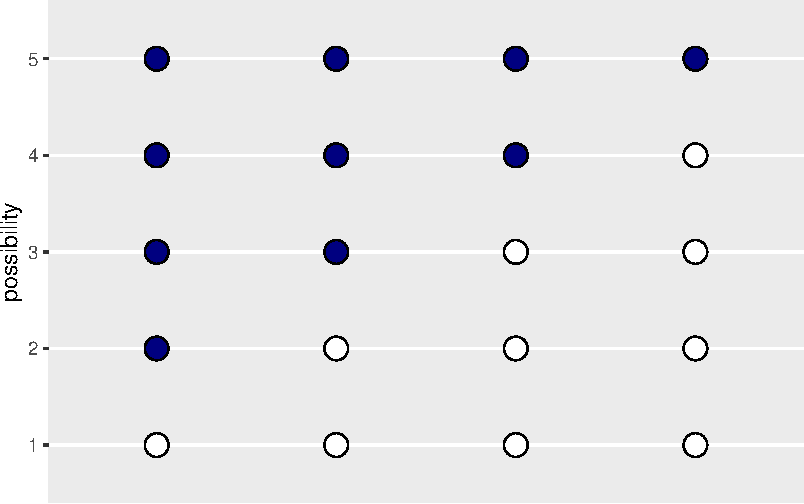
\includegraphics{02-small-and-large-worlds_files/figure-pdf/plot-possibilities-conjectures-1.pdf}

}

\end{figure}

\hypertarget{summarize-the-possiblity-structure}{%
\paragraph{Summarize the Possiblity
Structure}\label{summarize-the-possiblity-structure}}

\begin{quote}
Here's the basic structure of the possibilities per marble draw.
\end{quote}

\begin{Shaded}
\begin{Highlighting}[]
\InformationTok{\textasciigrave{}\textasciigrave{}\textasciigrave{}\{r\}}
\CommentTok{\#| label: tbl{-}basic{-}prob{-}struct}
\CommentTok{\#| tbl{-}cap: possibility{-}structure}

\FunctionTok{tibble}\NormalTok{(}\AttributeTok{draw    =} \DecValTok{1}\SpecialCharTok{:}\DecValTok{3}\NormalTok{,}
       \AttributeTok{marbles =} \DecValTok{4}\NormalTok{) }\SpecialCharTok{\%\textgreater{}\%} 
  \FunctionTok{mutate}\NormalTok{(}\AttributeTok{possibilities =}\NormalTok{ marbles }\SpecialCharTok{\^{}}\NormalTok{ draw) }\SpecialCharTok{\%\textgreater{}\%} 
\NormalTok{  kableExtra}\SpecialCharTok{::}\FunctionTok{kbl}\NormalTok{() }\SpecialCharTok{|\textgreater{}} 
\NormalTok{  kableExtra}\SpecialCharTok{::}\FunctionTok{kable\_classic}\NormalTok{(}\AttributeTok{full\_width =}\NormalTok{ F)}
\InformationTok{\textasciigrave{}\textasciigrave{}\textasciigrave{}}
\end{Highlighting}
\end{Shaded}

\hypertarget{tbl-basic-prob-struct}{}
\begin{table}
\caption{\label{tbl-basic-prob-struct}possibility-structure }\tabularnewline

\centering
\begin{tabular}[t]{r|r|r}
\hline
draw & marbles & possibilities\\
\hline
1 & 4 & 4\\
\hline
2 & 4 & 16\\
\hline
3 & 4 & 64\\
\hline
\end{tabular}
\end{table}

\begin{tcolorbox}[enhanced jigsaw, colframe=quarto-callout-note-color-frame, colback=white, toprule=.15mm, breakable, arc=.35mm, bottomtitle=1mm, colbacktitle=quarto-callout-note-color!10!white, toptitle=1mm, titlerule=0mm, title=\textcolor{quarto-callout-note-color}{\faInfo}\hspace{0.5em}{Table Packages Used}, leftrule=.75mm, opacityback=0, rightrule=.15mm, opacitybacktitle=0.6, bottomrule=.15mm, left=2mm, coltitle=black]

Kurz employed the \{\textbf{flextable}\} package to print tables. As I
have no experience with this package, I will apply
\{\textbf{kableExtra}\} in this document.\\
\strut \\
Until now I had used most of the time kableExtra and sometimes DT. For a
short compilation of available table packages see the section on
\href{https://bookdown.org/yihui/rmarkdown-cookbook/table-other.html}{Other
packages for creating tables} in the R Markdown Cookbook. The following
excursion on tables follows the blog article
\href{https://towardsdatascience.com/top-7-packages-for-making-beautiful-tables-in-r-7683d054e541}{Top
7 Packages for Making Beautiful Tables in R} by Devashree Madhugiri.

\end{tcolorbox}

\hypertarget{excursion-tables}{%
\subsubsection{Excursion: Tables}\label{excursion-tables}}

\begin{itemize}
\item
  \href{https://gt.rstudio.com/}{\{\textbf{gt}\}}: The gt package offers
  a different and easy-to-use set of functions that helps us build
  display tables from tabular data. The gt philosophy states that a
  comprehensive collection of table parts can be used to create a broad
  range of functional tables. These are the table body, the table
  footer, the spanner column labels, the column labels, and the table
  header. (I should look into the \{\textbf{gt}\} package in more detail
  as it is developed by the RStudio/Posit team, that stands not only for
  high quality but also for tidyverse compatibility.)

  \includesvg{index_files/mediabag/gt_parts_of_a_table.svg}
\item
  \href{https://renkun-ken.github.io/formattable/}{\{\textbf{formattable}\}}:
  Formattable data frames are data frames that will be displayed in HTML
  tables using formatter functions. This package includes techniques to
  produce data structures with predefined formatting rules, such that
  the objects maintain the original data but are formatted. The package
  consists of several standard formattable objects, including percent,
  comma, currency, accounting, and scientific.
\item
  \href{https://haozhu233.github.io/kableExtra/}{\{\textbf{kableExtra}\}}:
  It extends the basic functionality of \texttt{knitr::kable()} tables.
  Although \texttt{knitr::kable()} is simple by design, it has many
  features missing which are usually available in other packages.
  \{\textbf{kableExtra}\} has filled the gap nicely. One of the best
  thing about \{\textbf{kableExtra}\} is that most of its table
  capabilities work for both HTML and PDF formats.
\item
  \href{https://rstudio.github.io/DT/}{\{\textbf{DT}\}}: dt is an
  abbreviation of `DataTables.' Data objects in R can be rendered as
  HTML tables using the JavaScript library `DataTables' (typically via R
  Markdown or Shiny).
\item
  \href{https://davidgohel.github.io/flextable/}{\{\textbf{flextable}\}}:
  This package helps you to create reporting table from a data frame
  easily. You can merge cells, add headers, add footers, change
  formatting, and set how data in cells is displayed. Table content can
  also contain mixed types of text and image content. Tables can be
  embedded from R Markdown documents into HTML, PDF, Word, and
  PowerPoint documents and can be embedded using Package Officer for
  Microsoft Word or PowerPoint documents. Tables can also be exported as
  R plots or graphic files, e.g., png, pdf, and jpeg.
\item
  \href{https://glin.github.io/reactable/}{\{\textbf{reactable}\}}:
  \texttt{reactable()} creates a data table from tabular data with
  sorting and pagination by default. The data table is an HTML widget
  that can be used in R Markdown documents and Shiny applications or
  viewed from an R console. It is based on the React Table library and
  made with reactR. Features are:

  \begin{itemize}
  \tightlist
  \item
    It creates a data table with sorting, filtering, and pagination
  \item
    It has built-in column formatting
  \item
    It supports custom rendering via R or JavaScript
  \item
    It works seamlessly within R Markdown documents and the Shiny app
  \end{itemize}
\item
  \href{https://kcuilla.github.io/reactablefmtr/index.html}{\{\textbf{ractablefmtr}\}}:
  The package improves the appearance and formatting of tables created
  using the reactable R library. It includes many conditional formatters
  that are highly customizable and easy to use.
\end{itemize}

I sure there are other packages as well. But the above seven packages
are a first starting point to learn creating and displaying
sophisticated data tables in R.

\begin{quote}
The authors of R Markdown Cookbook (Yihui Xie, Christophe Dervieux,
Emily Riederer) mention also several other table packages in the section
\href{https://bookdown.org/yihui/rmarkdown-cookbook/table-other.html}{Other
packages for creating tables}:

\begin{itemize}
\item
  \textbf{rhandsontable}
  (\href{https://bookdown.org/yihui/rmarkdown-cookbook/table-other.html\#ref-R-rhandsontable}{Owen
  2021}): Also similar to \textbf{DT}, and has an Excel feel (e.g., you
  can edit data directly in the table). Visit
  \url{https://jrowen.github.io/rhandsontable/} to learn more about it.
\item
  \textbf{pixiedust}
  (\href{https://bookdown.org/yihui/rmarkdown-cookbook/table-other.html\#ref-R-pixiedust}{Nutter
  2021}): Features creating tables for models (such as linear models)
  converted through the \textbf{broom} package
  (\href{https://bookdown.org/yihui/rmarkdown-cookbook/table-other.html\#ref-R-broom}{Robinson,
  Hayes, and Couch 2023}). It supports Markdown, HTML, and LaTeX output
  formats. Its repository is at
  \url{https://github.com/nutterb/pixiedust}.
\item
  \textbf{stargazer}
  (\href{https://bookdown.org/yihui/rmarkdown-cookbook/table-other.html\#ref-R-stargazer}{Hlavac
  2022}): Features formatting regression models and summary statistics
  tables. The package is available on CRAN at
  \url{https://cran.r-project.org/package=stargazer}.
\item
  \textbf{xtable}
  (\href{https://bookdown.org/yihui/rmarkdown-cookbook/table-other.html\#ref-R-xtable}{Dahl
  et al. 2019}): Perhaps the oldest package for creating tables---the
  first release was made in 2000. It supports both LaTeX and HTML
  formats. The package is available on CRAN at
  \url{https://cran.r-project.org/package=xtable}.
\end{itemize}

I'm not going to introduce the rest of packages, but will just list them
here: \textbf{tables}
(\href{https://bookdown.org/yihui/rmarkdown-cookbook/table-other.html\#ref-R-tables}{Murdoch
2023}), \textbf{pander}
(\href{https://bookdown.org/yihui/rmarkdown-cookbook/table-other.html\#ref-R-pander}{Daróczi
and Tsegelskyi 2022}), \textbf{tangram}
(\href{https://bookdown.org/yihui/rmarkdown-cookbook/table-other.html\#ref-R-tangram}{S.
Garbett 2023}), \textbf{ztable}
(\href{https://bookdown.org/yihui/rmarkdown-cookbook/table-other.html\#ref-R-ztable}{Moon
2021}), and \textbf{condformat}
(\href{https://bookdown.org/yihui/rmarkdown-cookbook/table-other.html\#ref-R-condformat}{Oller
Moreno 2022}).
\end{quote}

\hypertarget{building-a-model}{%
\section{Building a Model}\label{building-a-model}}

\hypertarget{original-2}{%
\subsection{Original}\label{original-2}}

\textbf{Globe-tossing}

We are going to use a toy example, but it has the same structure as a
typical statistical analyses. The first nine samples produce the
following data:

\texttt{W\ L\ W\ W\ W\ L\ W\ L\ W} (W indicates water and L indicates
land.)

Designing a simple Bayesian model benefits from a design loop with three
steps.

\begin{enumerate}
\def\labelenumi{\arabic{enumi}.}
\tightlist
\item
  \textbf{Data story}: Motivate the model by narrating how the data
  might arise.
\item
  \textbf{Update}: Educate your model by feeding it the data.
\item
  \textbf{Evaluate}: All statistical models require supervision, leading
  to model revision.
\end{enumerate}

\hypertarget{a-data-story}{%
\subsubsection{A Data Story}\label{a-data-story}}

\begin{quote}
Bayesian data analysis usually means producing a story for how the data
came to be. This story may be \emph{descriptive}, specifying
associations that can be used to predict outcomes, given observations.
Or it may be \emph{causal}, a theory of how some events produce other
events.
\end{quote}

All data stories have to be complete in the sense that they are
sufficient for specifying an algorithm for simulating new data.

\begin{quote}
You can motivate your data story by trying to explain how each piece of
data is born. This usually means describing aspects of the underlying
reality as well as the sampling process. The data story in \ldots{}
{[}our toy case of globe-tossing{]} is simply a restatement of the
sampling process:

\begin{enumerate}
\def\labelenumi{\arabic{enumi}.}
\tightlist
\item
  The true proportion of water covering the globe is \emph{\texttt{p}}.
\item
  A single toss of the globe has a probability \emph{\texttt{p}} of
  producing a water (W) observation. It has a probability
  \texttt{1\ –\ p} of producing a land (L) observation.
\item
  Each toss of the globe is independent of the others.
\end{enumerate}
\end{quote}

\hypertarget{bayesian-updating}{%
\subsubsection{Bayesian Updating}\label{bayesian-updating}}

\begin{quote}
A Bayesian model begins with one set of plausibilities assigned to each
of these possibilities. These are the prior plausibilities. Then it
updates them in light of the data, to produce the posterior
plausibilities. This updating process is a kind of learning, called
\textbf{BAYESIAN UPDATING}.

\ldots{}

For the sake of the example only, let's program our Bayesian machine to
initially assign the same plausibility to every proportion of water,
every value of \emph{p}. We'll do better than this later.

\ldots{}

Every time a ``W'' is seen, the peak of the plausibility curve moves to
the right, towards larger values of \emph{p}. Every time an ``L'' is
seen, it moves the other direction. The maximum height of the curve
increases with each sample, meaning that fewer values of \emph{p} amass
more plausibility as the amount of evidence increases. As each new
observation is added, the curve is updated consistent with all previous
observations.
\end{quote}

To see the results of the different (updating) steps I am going to
reproduce Figure 2.5 (How a Bayesian model learns) of the book. In the
tidyverse-version we will learn how to write R code to reproduce the
graphic.

\begin{figure}

{\centering 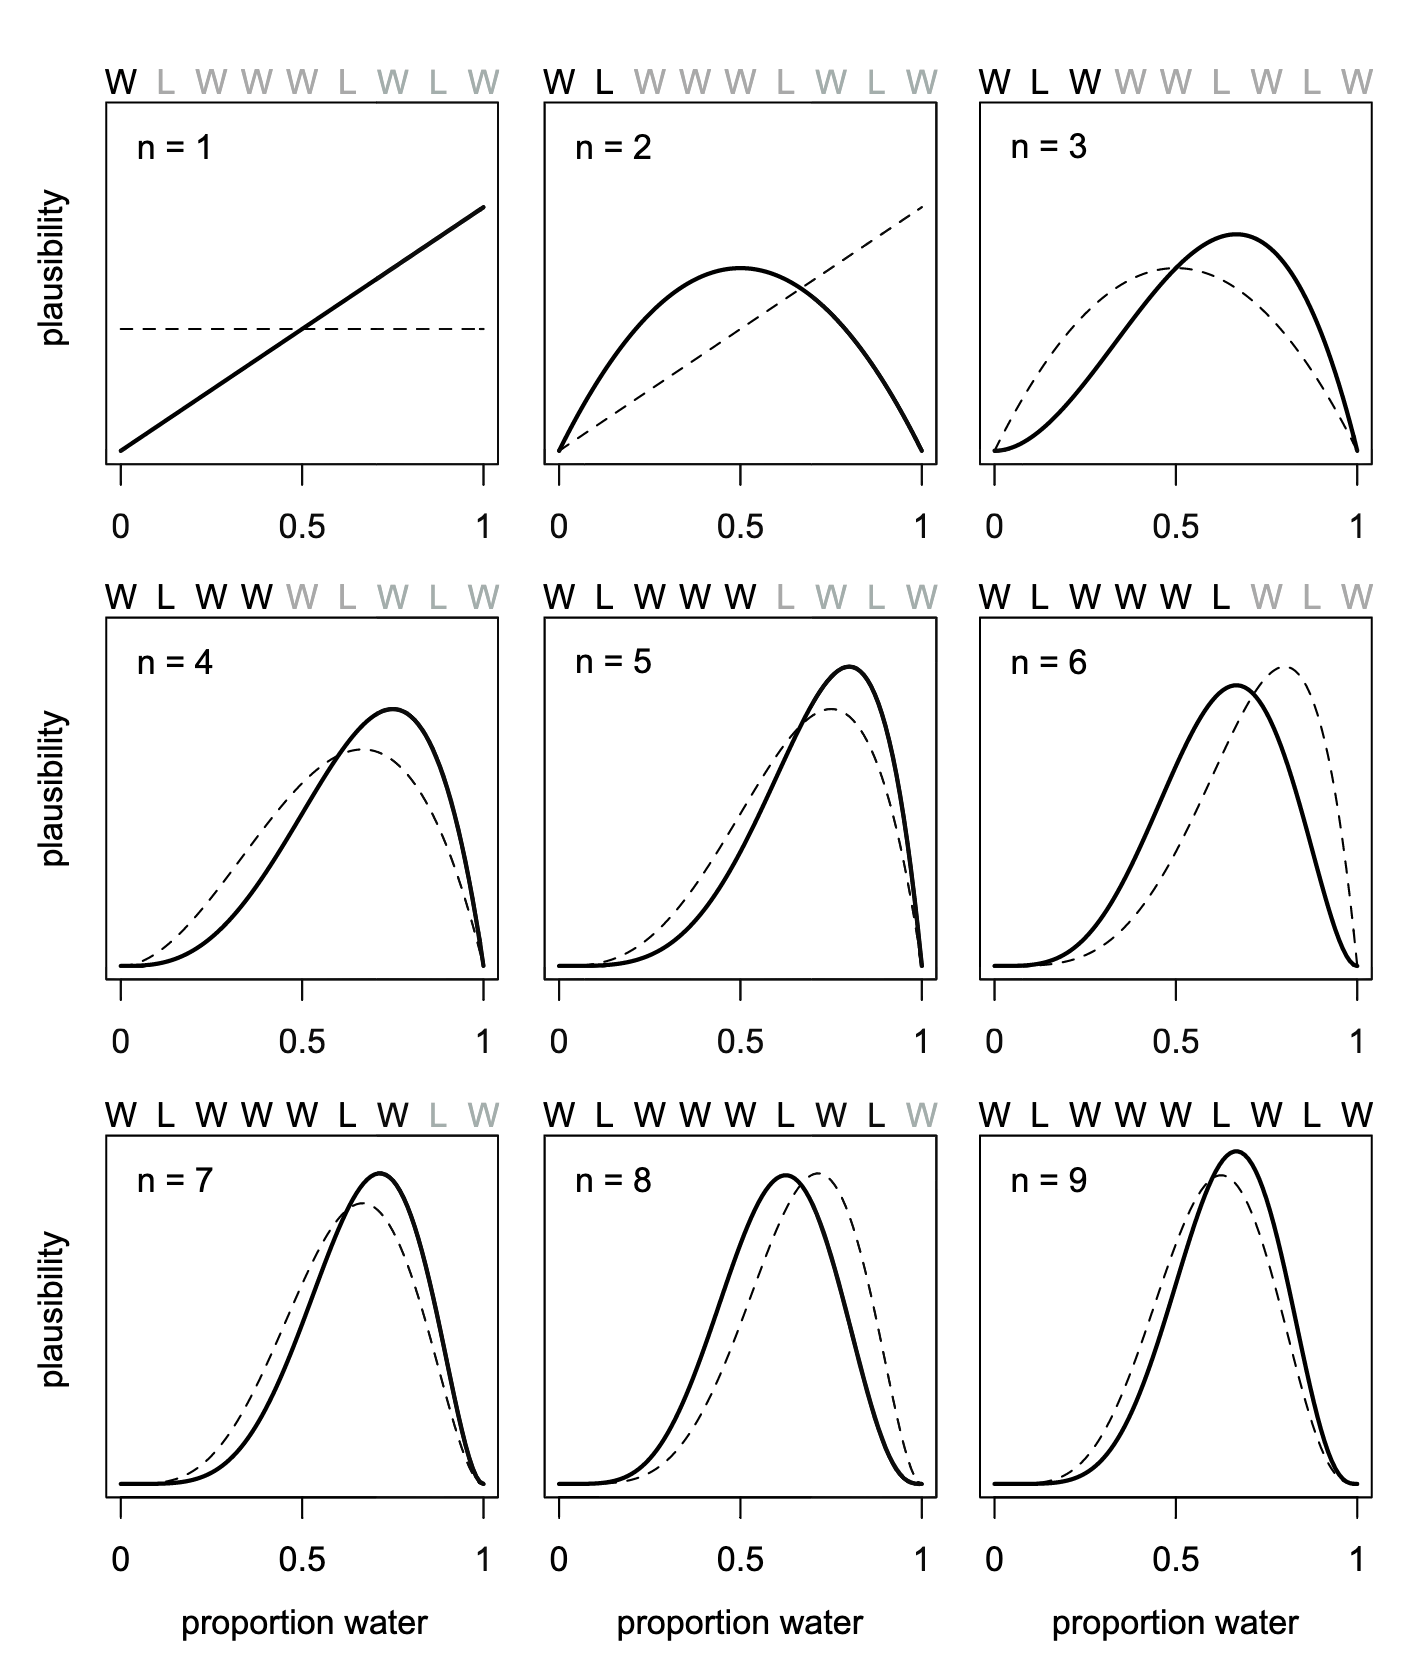
\includegraphics{img/bayesian_model_learns_step_by_step-min.png}

}

\caption{\label{fig-2-5-book-copy}Copy of Figure 2.5: \textbf{How a
Bayesian model learns}. In each plot, previous plausibilities (dashed
curve) are updated in light of the latest observation to produce a new
set of plausibilities (solid curve).}

\end{figure}

\hypertarget{evaluate}{%
\subsubsection{Evaluate}\label{evaluate}}

Keep in mind two cautious principles:

\begin{enumerate}
\def\labelenumi{\arabic{enumi}.}
\item
  \begin{quote}
  \begin{itemize}
  \item
    First, \textbf{the model's certainty is no guarantee that the model
    is a good one}. \ldots{} {[}M{]}odels of all sorts---Bayesian or
    not---can be very confident about an inference, even when the model
    is seriously misleading. This is because the inferences are
    conditional on the model. What your model is telling you is that,
    given a commitment to this particular model, it can be very sure
    that the plausible values are in a narrow range. Under a different
    model, things might look differently.
  \item
    Second, \textbf{it is important to supervise and critique your
    model's work}. \ldots{} When something is irrelevant to the machine,
    it won't affect the inference directly. But it may affect it
    indirectly \ldots{} So it is important to check the model's
    inferences in light of aspects of the data it does not know about.
    Such checks are an inherently creative enterprise, left to the
    analyst and the scientific community. Golems are very bad at it.
    (emphasis pb)
  \end{itemize}
  \end{quote}
\end{enumerate}

Further keep in mind that

\begin{quote}
the goal is not to test the truth value of the model's assumptions. We
know the model's assumptions are never exactly right, in the sense of
matching the true data generating process. \ldots{} Moreover, models do
not need to be exactly true in order to produce highly precise and
useful inferences.

Instead, the objective is to check the model's adequacy for some
purpose. This usually means asking and answering additional questions,
beyond those that originally constructed the model. Both the questions
and answers will depend upon the scientific context. So it's hard to
provide general advice.
\end{quote}

\hypertarget{video}{%
\subsection{Video}\label{video}}

\hypertarget{bayesian-probability-of-the-water-proportion}{%
\subsubsection{Bayesian Probability of the Water
Proportion}\label{bayesian-probability-of-the-water-proportion}}

\href{https://speakerdeck.com/rmcelreath/statistical-rethinking-2023-lecture-02?slide=50}{R
Code snippet 2.1}: Statistical Rethinking 2023 - Lecture 02, Slide 50.

\begin{Shaded}
\begin{Highlighting}[]
\InformationTok{\textasciigrave{}\textasciigrave{}\textasciigrave{}\{r\}}
\CommentTok{\#| label: probability{-}water}

\NormalTok{sample }\OtherTok{\textless{}{-}} \FunctionTok{c}\NormalTok{(}\StringTok{"W"}\NormalTok{, }\StringTok{"L"}\NormalTok{, }\StringTok{"W"}\NormalTok{, }\StringTok{"W"}\NormalTok{, }\StringTok{"W"}\NormalTok{, }\StringTok{"L"}\NormalTok{, }\StringTok{"W"}\NormalTok{, }\StringTok{"L"}\NormalTok{, }\StringTok{"W"}\NormalTok{)}
\NormalTok{W }\OtherTok{\textless{}{-}} \FunctionTok{sum}\NormalTok{(sample }\SpecialCharTok{==} \StringTok{"W"}\NormalTok{) }\CommentTok{\# number of W observed}
\NormalTok{L }\OtherTok{\textless{}{-}} \FunctionTok{sum}\NormalTok{(sample }\SpecialCharTok{==} \StringTok{"L"}\NormalTok{) }\CommentTok{\# number of L observed}
\NormalTok{p }\OtherTok{\textless{}{-}} \FunctionTok{c}\NormalTok{(}\DecValTok{0}\NormalTok{, }\FloatTok{0.25}\NormalTok{, }\FloatTok{0.5}\NormalTok{, }\FloatTok{0.75}\NormalTok{, }\DecValTok{1}\NormalTok{) }\CommentTok{\# proportions W}

\CommentTok{\# using vectorized version instead of sapply()}
\CommentTok{\# see: https://github.com/rmcelreath/stat\_rethinking\_2023/issues/6}
\NormalTok{get\_ways }\OtherTok{\textless{}{-}} \ControlFlowTok{function}\NormalTok{(q) (q }\SpecialCharTok{*} \DecValTok{4}\NormalTok{)}\SpecialCharTok{\^{}}\NormalTok{W }\SpecialCharTok{*}\NormalTok{ ((}\DecValTok{1} \SpecialCharTok{{-}}\NormalTok{ q) }\SpecialCharTok{*} \DecValTok{4}\NormalTok{)}\SpecialCharTok{\^{}}\NormalTok{L}
\NormalTok{ways }\OtherTok{\textless{}{-}} \FunctionTok{get\_ways}\NormalTok{(p)}
\NormalTok{prob }\OtherTok{\textless{}{-}}\NormalTok{ ways }\SpecialCharTok{/} \FunctionTok{sum}\NormalTok{(ways)}
\FunctionTok{cbind}\NormalTok{(p, ways, prob)}
\InformationTok{\textasciigrave{}\textasciigrave{}\textasciigrave{}}
\end{Highlighting}
\end{Shaded}

\begin{verbatim}
#>         p ways       prob
#> [1,] 0.00    0 0.00000000
#> [2,] 0.25   27 0.02129338
#> [3,] 0.50  512 0.40378549
#> [4,] 0.75  729 0.57492114
#> [5,] 1.00    0 0.00000000
\end{verbatim}

\texttt{prob} is called the \textbf{posterior distribution} because it's
posterior to the sample to the updating we did in light of the data.

This estimator is optimal you cannot do better than this if your model
is correct and the model here doesn't mean the particular value of P -
it means the generative hypothesis about how the garden is drawn given a
particular value of P.

\hypertarget{test-before-you-estimate}{%
\subsubsection{Test Before You
Est(imate)}\label{test-before-you-estimate}}

In the planned third version of the book McElreath wants to include from
the beginning the evaluation part of the process. It is mentioned in the
book already in this chapter 2 but without practical implementation and
code examples. But we can find some remarks in his
\href{https://www.youtube.com/playlist?list=PLDcUM9US4XdPz-KxHM4XHt7uUVGWWVSus}{Statistical
Rethinking Videos 2023}.

\begin{quote}
We want to worry about the correctness of code in scientific data
analysis as well because scientific data analysis is in the vast
majority of fields a kind of amateur software development. There is
scripting and we want to document our code and we need to worry about
errors and want to have a reliable workflow that does some quality
assurance. So we've coded a generative simulation and we've coded an
estimator and now we'd like to test our estimator with our generative
simulation.
(\href{https://www.youtube.com/watch?v=R1vcdhPBlXA&list=PLDcUM9US4XdPz-KxHM4XHt7uUVGWWVSus&index=2&t=37m40s}{37:40})
\end{quote}

\begin{enumerate}
\def\labelenumi{\arabic{enumi}.}
\tightlist
\item
  Code a generative simulation
\item
  Code an estimator
\item
  Test (2) with (1)
\end{enumerate}

\hypertarget{simulating-the-globe-tossing}{%
\paragraph{Simulating the Globe
Tossing}\label{simulating-the-globe-tossing}}

\begin{figure}

{\centering 

\href{https://speakerdeck.com/rmcelreath/statistical-rethinking-2023-lecture-02?slide=54}{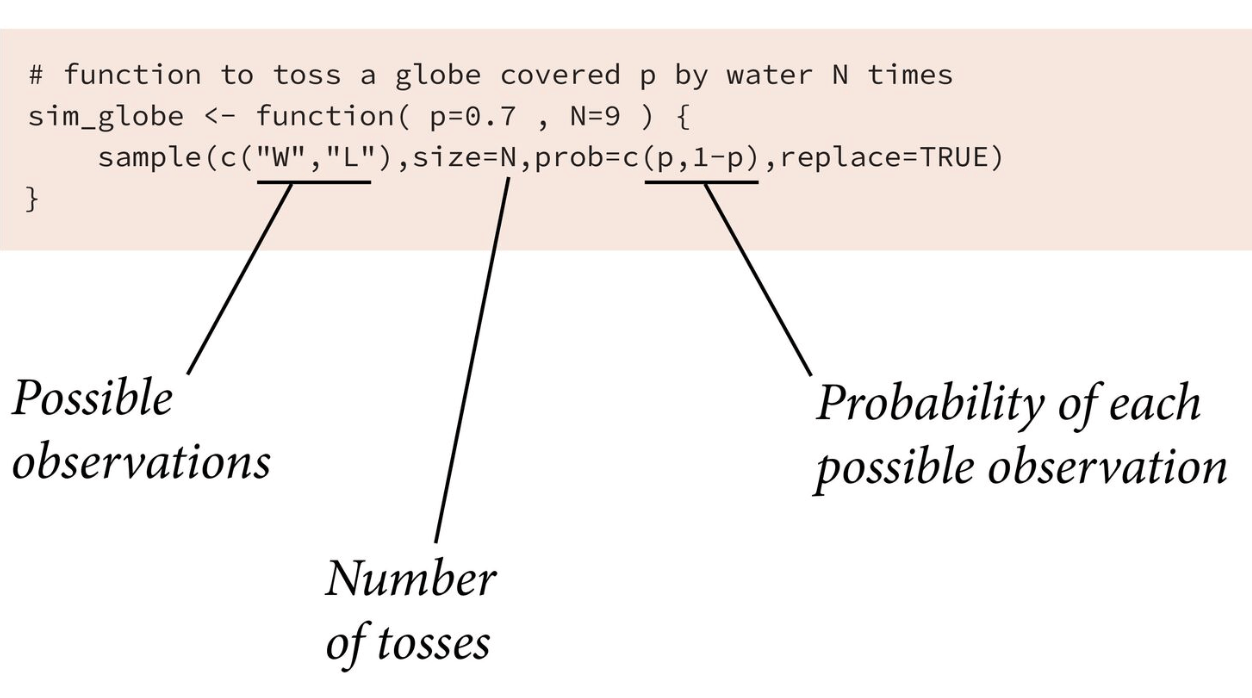
\includegraphics{img/code-sim-globe-tossing-min.png}}

}

\caption{R Code 2.3, Statistical Rethinking 2023 - Lecture 02, {[}Slide
54{]}(https://speakerdeck.com/rmcelreath/statistical-rethinking-2023-lecture-02?slide=54).}

\end{figure}

\begin{Shaded}
\begin{Highlighting}[]
\InformationTok{\textasciigrave{}\textasciigrave{}\textasciigrave{}\{r\}}
\CommentTok{\#| label: sim{-}globe{-}tossing}

\CommentTok{\# function to toss a globe covered p by water N times}
\NormalTok{sim\_globe }\OtherTok{\textless{}{-}} \ControlFlowTok{function}\NormalTok{(}\AttributeTok{p =} \FloatTok{0.7}\NormalTok{, }\AttributeTok{N =} \DecValTok{9}\NormalTok{) \{}
  \FunctionTok{sample}\NormalTok{(}\FunctionTok{c}\NormalTok{(}\StringTok{"W"}\NormalTok{, }\StringTok{"L"}\NormalTok{), }\AttributeTok{size =}\NormalTok{ N, }\AttributeTok{prob =} \FunctionTok{c}\NormalTok{(p, }\DecValTok{1} \SpecialCharTok{{-}}\NormalTok{ p), }\AttributeTok{replace =} \ConstantTok{TRUE}\NormalTok{)}
\NormalTok{\}}
\FunctionTok{sim\_globe}\NormalTok{()}
\InformationTok{\textasciigrave{}\textasciigrave{}\textasciigrave{}}
\end{Highlighting}
\end{Shaded}

\begin{verbatim}
#> [1] "W" "W" "W" "L" "L" "W" "W" "W" "W"
\end{verbatim}

You can simulate the experiment arbitrary times for any particular
proportion of water you like. This is a way to explore the design of an
experiment as well as debug the code.
(\href{https://www.youtube.com/watch?v=R1vcdhPBlXA&list=PLDcUM9US4XdPz-KxHM4XHt7uUVGWWVSus&index=2&t=39m55s}{39:55}).

\begin{Shaded}
\begin{Highlighting}[]
\InformationTok{\textasciigrave{}\textasciigrave{}\textasciigrave{}\{r\}}
\CommentTok{\#| label: replicate{-}sim}
\CommentTok{\#| lst{-}cap: "R code snippet 2.4: Replicate simulation"}

\CommentTok{\# replicate simulation 10 times with different p values (here: p = 0.5)}
\FunctionTok{replicate}\NormalTok{(}\FunctionTok{sim\_globe}\NormalTok{(}\AttributeTok{p =} \FloatTok{0.5}\NormalTok{, }\AttributeTok{N =} \DecValTok{9}\NormalTok{), }\AttributeTok{n =} \DecValTok{10}\NormalTok{) }
\InformationTok{\textasciigrave{}\textasciigrave{}\textasciigrave{}}
\end{Highlighting}
\end{Shaded}

\begin{verbatim}
#>       [,1] [,2] [,3] [,4] [,5] [,6] [,7] [,8] [,9] [,10]
#>  [1,] "L"  "L"  "W"  "W"  "L"  "L"  "W"  "L"  "W"  "L"  
#>  [2,] "L"  "W"  "W"  "W"  "L"  "W"  "L"  "L"  "W"  "W"  
#>  [3,] "L"  "W"  "W"  "W"  "L"  "W"  "W"  "W"  "L"  "L"  
#>  [4,] "W"  "L"  "W"  "W"  "L"  "L"  "W"  "L"  "W"  "W"  
#>  [5,] "L"  "W"  "W"  "W"  "W"  "L"  "L"  "L"  "L"  "L"  
#>  [6,] "W"  "L"  "W"  "L"  "L"  "L"  "L"  "L"  "L"  "W"  
#>  [7,] "W"  "L"  "W"  "W"  "L"  "W"  "L"  "W"  "L"  "W"  
#>  [8,] "W"  "L"  "W"  "W"  "L"  "W"  "W"  "L"  "W"  "L"  
#>  [9,] "W"  "L"  "L"  "W"  "L"  "W"  "L"  "W"  "W"  "L"
\end{verbatim}

\begin{tcolorbox}[enhanced jigsaw, colframe=quarto-callout-warning-color-frame, colback=white, toprule=.15mm, breakable, arc=.35mm, bottomtitle=1mm, colbacktitle=quarto-callout-warning-color!10!white, toptitle=1mm, titlerule=0mm, title=\textcolor{quarto-callout-warning-color}{\faExclamationTriangle}\hspace{0.5em}{Quarto cannot list \& execute code in the same chunk}, leftrule=.75mm, opacityback=0, rightrule=.15mm, opacitybacktitle=0.6, bottomrule=.15mm, left=2mm, coltitle=black]

2023-05-08: \texttt{lst-label} and \texttt{lst-cap} are only working in
display code snippets but not in snippets to execute. See
\href{https://community.rstudio.com/t/lst-cap-and-lst-label-in-quarto/157173}{lst-cap
and lst-label in Quarto?} and
\href{https://github.com/quarto-dev/quarto-cli/issues/1580}{lst-label
and lst-cap do not produce listing caption and reference}.

\end{tcolorbox}

2023-07-23: In the meanwhile I found a work around:

\begin{codelisting}

\caption{R code snippet 2.4: Replicate simulation}

\hypertarget{lst-replicate-sim2}{%
\label{lst-replicate-sim2}}%
\begin{Shaded}
\begin{Highlighting}[]
\InformationTok{\textasciigrave{}\textasciigrave{}\textasciigrave{}\{r\}}
\CommentTok{\#| label: replicate{-}sim2}
\CommentTok{\#| attr{-}source: \textquotesingle{}\#lst{-}replicate{-}sim2 lst{-}cap="R code snippet 2.4: Replicate simulation"\textquotesingle{}}

\FunctionTok{replicate}\NormalTok{(}\FunctionTok{sim\_globe}\NormalTok{(}\AttributeTok{p =} \FloatTok{0.5}\NormalTok{, }\AttributeTok{N =} \DecValTok{9}\NormalTok{), }\AttributeTok{n =} \DecValTok{10}\NormalTok{) }
\InformationTok{\textasciigrave{}\textasciigrave{}\textasciigrave{}}
\end{Highlighting}
\end{Shaded}

\end{codelisting}

\begin{verbatim}
#>       [,1] [,2] [,3] [,4] [,5] [,6] [,7] [,8] [,9] [,10]
#>  [1,] "W"  "W"  "L"  "L"  "L"  "L"  "W"  "W"  "L"  "L"  
#>  [2,] "L"  "L"  "W"  "W"  "W"  "L"  "L"  "W"  "L"  "L"  
#>  [3,] "W"  "W"  "W"  "L"  "W"  "L"  "W"  "L"  "L"  "L"  
#>  [4,] "L"  "W"  "W"  "W"  "L"  "W"  "L"  "L"  "L"  "L"  
#>  [5,] "L"  "W"  "W"  "W"  "L"  "W"  "L"  "W"  "L"  "W"  
#>  [6,] "L"  "L"  "L"  "L"  "L"  "L"  "L"  "L"  "L"  "L"  
#>  [7,] "W"  "W"  "W"  "W"  "L"  "W"  "L"  "W"  "L"  "L"  
#>  [8,] "L"  "W"  "L"  "L"  "W"  "L"  "L"  "L"  "W"  "W"  
#>  [9,] "L"  "L"  "L"  "L"  "W"  "W"  "W"  "W"  "W"  "L"
\end{verbatim}

\hypertarget{test-the-simulation-at-extreme-values}{%
\paragraph{Test the simulation at extreme
values}\label{test-the-simulation-at-extreme-values}}

R code snippets 2.5 and 2.6:
\href{https://speakerdeck.com/rmcelreath/statistical-rethinking-2023-lecture-02?slide=57}{Slide
57}.

\begin{Shaded}
\begin{Highlighting}[]
\InformationTok{\textasciigrave{}\textasciigrave{}\textasciigrave{}\{r\}}
\CommentTok{\#| label: test{-}sim{-}extrem{-}values}
\FunctionTok{sim\_globe}\NormalTok{(}\AttributeTok{p =} \DecValTok{1}\NormalTok{, }\AttributeTok{N =} \DecValTok{10}\NormalTok{) }\CommentTok{\# test, when p = 1}

\FunctionTok{sum}\NormalTok{(}\FunctionTok{sim\_globe}\NormalTok{(}\AttributeTok{p =} \FloatTok{0.5}\NormalTok{, }\AttributeTok{N =} \FloatTok{1e4}\NormalTok{) }\SpecialCharTok{==} \StringTok{"W"}\NormalTok{) }\SpecialCharTok{/} \FloatTok{1e4} \CommentTok{\# test 1e4 (10.000) times}
\InformationTok{\textasciigrave{}\textasciigrave{}\textasciigrave{}}
\end{Highlighting}
\end{Shaded}

\begin{verbatim}
#>  [1] "W" "W" "W" "W" "W" "W" "W" "W" "W" "W"
#> [1] 0.5114
\end{verbatim}

\hypertarget{code-an-estimator-and-test-it-with-the-simulation}{%
\paragraph{Code an estimator and test it with the
simulation}\label{code-an-estimator-and-test-it-with-the-simulation}}

In the following compute\_posterior() function I could not manage to get
working the part with the bars. As far as I understand it comes from the
\texttt{animint} or \texttt{animint2} package but I did not know how to
fill in the second required parameter \texttt{x.name}.

\begin{Shaded}
\begin{Highlighting}[]
\InformationTok{\textasciigrave{}\textasciigrave{}\textasciigrave{}\{r\}}
\CommentTok{\#| label: test{-}est{-}with{-}sim}

\CommentTok{\# function to compute posterior distribution }
\NormalTok{compute\_posterior }\OtherTok{\textless{}{-}} \ControlFlowTok{function}\NormalTok{(the\_sample, }\AttributeTok{poss =} \FunctionTok{c}\NormalTok{(}\DecValTok{0}\NormalTok{, }\FloatTok{0.25}\NormalTok{, }\FloatTok{0.5}\NormalTok{, }\FloatTok{0.75}\NormalTok{, }\DecValTok{1}\NormalTok{)) \{}
\NormalTok{  W }\OtherTok{\textless{}{-}} \FunctionTok{sum}\NormalTok{(the\_sample }\SpecialCharTok{==} \StringTok{"W"}\NormalTok{) }\CommentTok{\# number of W observed}
\NormalTok{  L }\OtherTok{\textless{}{-}} \FunctionTok{sum}\NormalTok{(the\_sample }\SpecialCharTok{==} \StringTok{"L"}\NormalTok{) }\CommentTok{\# number of L observed}
\NormalTok{  get\_ways }\OtherTok{\textless{}{-}} \ControlFlowTok{function}\NormalTok{(q) (q }\SpecialCharTok{*} \DecValTok{4}\NormalTok{)}\SpecialCharTok{\^{}}\NormalTok{W }\SpecialCharTok{*}\NormalTok{ ((}\DecValTok{1} \SpecialCharTok{{-}}\NormalTok{ q) }\SpecialCharTok{*} \DecValTok{4}\NormalTok{)}\SpecialCharTok{\^{}}\NormalTok{L}
\NormalTok{  ways }\OtherTok{\textless{}{-}} \FunctionTok{get\_ways}\NormalTok{(poss)}
  \CommentTok{\# ways \textless{}{-} sapply(poss, function(q) (q * 4)\^{}W * ((1 {-} q) * 4)\^{}L)}
\NormalTok{  post }\OtherTok{\textless{}{-}}\NormalTok{ ways }\SpecialCharTok{/} \FunctionTok{sum}\NormalTok{(ways)}
  \CommentTok{\# cannot find second parameter of function make\_bar()}
  \CommentTok{\# bars \textless{}{-} sapply(post, function(q) animint2::make\_bar(q)) }
  \FunctionTok{data.frame}\NormalTok{(poss, ways, }\AttributeTok{post =} \FunctionTok{round}\NormalTok{(post, }\DecValTok{3}\NormalTok{))}
\NormalTok{\}}

\FunctionTok{compute\_posterior}\NormalTok{(}\FunctionTok{sim\_globe}\NormalTok{())}
\InformationTok{\textasciigrave{}\textasciigrave{}\textasciigrave{}}
\end{Highlighting}
\end{Shaded}

\begin{verbatim}
#>   poss ways  post
#> 1 0.00    0 0.000
#> 2 0.25    9 0.003
#> 3 0.50  512 0.189
#> 4 0.75 2187 0.808
#> 5 1.00    0 0.000
\end{verbatim}

\hypertarget{summary}{%
\paragraph{Summary}\label{summary}}

\begin{enumerate}
\def\labelenumi{\arabic{enumi}.}
\tightlist
\item
  Test the estimator where the answer is known
\item
  Explore different sampling designs
\item
  Develop intuition for sampling and estimation
\end{enumerate}

\hypertarget{tidyverse-2}{%
\subsection{Tidyverse}\label{tidyverse-2}}

Let's save our globe-tossing data \texttt{W\ L\ W\ W\ W\ L\ W\ L\ W} in
a tibble:

\begin{Shaded}
\begin{Highlighting}[]
\InformationTok{\textasciigrave{}\textasciigrave{}\textasciigrave{}\{r\}}
\CommentTok{\#| label: globe{-}tossing{-}data}

\NormalTok{(d }\OtherTok{\textless{}{-}} \FunctionTok{tibble}\NormalTok{(}\AttributeTok{toss =} \FunctionTok{c}\NormalTok{(}\StringTok{"w"}\NormalTok{, }\StringTok{"l"}\NormalTok{, }\StringTok{"w"}\NormalTok{, }\StringTok{"w"}\NormalTok{, }\StringTok{"w"}\NormalTok{, }\StringTok{"l"}\NormalTok{, }\StringTok{"w"}\NormalTok{, }\StringTok{"l"}\NormalTok{, }\StringTok{"w"}\NormalTok{)))}
\InformationTok{\textasciigrave{}\textasciigrave{}\textasciigrave{}}
\end{Highlighting}
\end{Shaded}

\begin{verbatim}
#> # A tibble: 9 x 1
#>   toss 
#>   <chr>
#> 1 w    
#> 2 l    
#> 3 w    
#> 4 w    
#> 5 w    
#> 6 l    
#> 7 w    
#> 8 l    
#> 9 w
\end{verbatim}

\hypertarget{a-data-story-1}{%
\subsubsection{A Data Story}\label{a-data-story-1}}

\hypertarget{sec-expand_grid}{%
\subsubsection{Bayesian Updating}\label{sec-expand_grid}}

For the updating process we need to add to the data the cumulative
number of trials, \texttt{n\_trials}, and the cumulative number of
successes, \texttt{n\_successes} (i.e., \texttt{toss\ ==\ "w"}).

\begin{Shaded}
\begin{Highlighting}[]
\InformationTok{\textasciigrave{}\textasciigrave{}\textasciigrave{}\{r\}}
\CommentTok{\#| label: bayesian{-}updating{-}start}

\NormalTok{(}
\NormalTok{  d }\OtherTok{\textless{}{-}}
\NormalTok{  d }\SpecialCharTok{\%\textgreater{}\%} 
  \FunctionTok{mutate}\NormalTok{(}\AttributeTok{n\_trials  =} \DecValTok{1}\SpecialCharTok{:}\DecValTok{9}\NormalTok{,}
         \AttributeTok{n\_success =} \FunctionTok{cumsum}\NormalTok{(toss }\SpecialCharTok{==} \StringTok{"w"}\NormalTok{))}
\NormalTok{  )}
\InformationTok{\textasciigrave{}\textasciigrave{}\textasciigrave{}}
\end{Highlighting}
\end{Shaded}

\begin{verbatim}
#> # A tibble: 9 x 3
#>   toss  n_trials n_success
#>   <chr>    <int>     <int>
#> 1 w            1         1
#> 2 l            2         1
#> 3 w            3         2
#> 4 w            4         3
#> 5 w            5         4
#> 6 l            6         4
#> 7 w            7         5
#> 8 l            8         5
#> 9 w            9         6
\end{verbatim}

The program code for reproducing the Figure 2.5 of the book (here in in
this document it is Picture~\ref{fig-2-5-book-copy}) is pretty complex.
Again I have to inspect the results line by line as I had done for the
Listing~\ref{lst-marble-data}. At first I will give a short introduction
what each line does. In the next steps I will explain each step more in
detail and show the result of the corresponding lines of code.

\begin{tcolorbox}[enhanced jigsaw, colframe=quarto-callout-warning-color-frame, colback=white, toprule=.15mm, breakable, arc=.35mm, bottomtitle=1mm, colbacktitle=quarto-callout-warning-color!10!white, toptitle=1mm, titlerule=0mm, title=\textcolor{quarto-callout-warning-color}{\faExclamationTriangle}\hspace{0.5em}{Preliminary Explanation of the Next Graph}, leftrule=.75mm, opacityback=0, rightrule=.15mm, opacitybacktitle=0.6, bottomrule=.15mm, left=2mm, coltitle=black]

The grid approximation used for the Bayesian updating in the next graph
are explained later in this chapter.\#

In the meanwhile I called the code from the following code chunk line by
line and inspected the result to understand what it does.

\end{tcolorbox}

\begin{tcolorbox}[enhanced jigsaw, colframe=quarto-callout-note-color-frame, colback=white, toprule=.15mm, breakable, arc=.35mm, bottomtitle=1mm, colbacktitle=quarto-callout-note-color!10!white, toptitle=1mm, titlerule=0mm, title=\textcolor{quarto-callout-note-color}{\faInfo}\hspace{0.5em}{Changed parameter name}, leftrule=.75mm, opacityback=0, rightrule=.15mm, opacitybacktitle=0.6, bottomrule=.15mm, left=2mm, coltitle=black]

In the following listing I had to change in the \texttt{lag()} function
the parameter \texttt{k} of the Kurz'sche version to \texttt{default} as
it is described in the corresponding
\href{https://dplyr.tidyverse.org/reference/lead-lag.html}{help file}. I
don't understand why \texttt{k}`was used. Maybe \texttt{k} was the name
of the parameter of a previous \{\textbf{dplyr}\} version?

\end{tcolorbox}

\hypertarget{annotated-cell-27}{%
\label{annotated-cell-27}}%
\begin{Shaded}
\begin{Highlighting}[]
\InformationTok{\textasciigrave{}\textasciigrave{}\textasciigrave{}\{r\}}
\CommentTok{\#| label: fig{-}bayesian{-}model{-}learning}
\CommentTok{\#| fig{-}cap: "How a Bayesian model learns"}
\CommentTok{\#| code{-}summary: "Code: **How a Bayesian model learns**"}

\CommentTok{\# starting data}
\NormalTok{d }\OtherTok{\textless{}{-}} \FunctionTok{tibble}\NormalTok{(}\AttributeTok{toss =} \FunctionTok{c}\NormalTok{(}\StringTok{"w"}\NormalTok{, }\StringTok{"l"}\NormalTok{, }\StringTok{"w"}\NormalTok{, }\StringTok{"w"}\NormalTok{, }\StringTok{"w"}\NormalTok{, }\StringTok{"l"}\NormalTok{, }\StringTok{"w"}\NormalTok{, }\StringTok{"l"}\NormalTok{, }\StringTok{"w"}\NormalTok{)) }\SpecialCharTok{|\textgreater{}} 
    \FunctionTok{mutate}\NormalTok{(}\AttributeTok{n\_trials  =} \DecValTok{1}\SpecialCharTok{:}\DecValTok{9}\NormalTok{, }\AttributeTok{n\_success =} \FunctionTok{cumsum}\NormalTok{(toss }\SpecialCharTok{==} \StringTok{"w"}\NormalTok{))}

\NormalTok{sequence\_length }\OtherTok{\textless{}{-}} \DecValTok{50} \hspace*{\fill}\NormalTok{\circled{1}}

\NormalTok{d }\SpecialCharTok{\%\textgreater{}\%} 
  \FunctionTok{expand\_grid}\NormalTok{(}\AttributeTok{p\_water =} \FunctionTok{seq}\NormalTok{(}\AttributeTok{from =} \DecValTok{0}\NormalTok{, }\AttributeTok{to =} \DecValTok{1}\NormalTok{, }
                            \AttributeTok{length.out =}\NormalTok{ sequence\_length)) }\SpecialCharTok{\%\textgreater{}\%} 
  \FunctionTok{group\_by}\NormalTok{(p\_water) }\SpecialCharTok{\%\textgreater{}\%} \hspace*{\fill}\NormalTok{\circled{2}}
  \FunctionTok{mutate}\NormalTok{(}\AttributeTok{lagged\_n\_trials  =} \FunctionTok{lag}\NormalTok{(n\_trials, }\AttributeTok{default =} \DecValTok{1}\NormalTok{),}
         \AttributeTok{lagged\_n\_success =} \FunctionTok{lag}\NormalTok{(n\_success, }\AttributeTok{default =} \DecValTok{1}\NormalTok{)) }\SpecialCharTok{\%\textgreater{}\%} \hspace*{\fill}\NormalTok{\circled{3}}
  \FunctionTok{ungroup}\NormalTok{() }\SpecialCharTok{\%\textgreater{}\%} \hspace*{\fill}\NormalTok{\circled{4}}
  \FunctionTok{mutate}\NormalTok{(}\AttributeTok{prior      =} \FunctionTok{ifelse}\NormalTok{(n\_trials }\SpecialCharTok{==} \DecValTok{1}\NormalTok{, .}\DecValTok{5}\NormalTok{,}
                             \FunctionTok{dbinom}\NormalTok{(}\AttributeTok{x    =}\NormalTok{ lagged\_n\_success, }
                                    \AttributeTok{size =}\NormalTok{ lagged\_n\_trials, }
                                    \AttributeTok{prob =}\NormalTok{ p\_water)),}
         \AttributeTok{likelihood =} \FunctionTok{dbinom}\NormalTok{(}\AttributeTok{x    =}\NormalTok{ n\_success, }
                             \AttributeTok{size =}\NormalTok{ n\_trials, }
                             \AttributeTok{prob =}\NormalTok{ p\_water),}
         \AttributeTok{strip      =} \FunctionTok{str\_c}\NormalTok{(}\StringTok{"n = "}\NormalTok{, n\_trials)) }\SpecialCharTok{\%\textgreater{}\%} \hspace*{\fill}\NormalTok{\circled{5}}
  
  \CommentTok{\# normalize prior and likelihood }
  \FunctionTok{group\_by}\NormalTok{(n\_trials) }\SpecialCharTok{\%\textgreater{}\%} \hspace*{\fill}\NormalTok{\circled{6}}
  \FunctionTok{mutate}\NormalTok{(}\AttributeTok{prior      =}\NormalTok{ prior }\SpecialCharTok{/} \FunctionTok{sum}\NormalTok{(prior),}
         \AttributeTok{likelihood =}\NormalTok{ likelihood }\SpecialCharTok{/} \FunctionTok{sum}\NormalTok{(likelihood)) }\SpecialCharTok{\%\textgreater{}\%} 
  
  \CommentTok{\# plot the result}
  \FunctionTok{ggplot}\NormalTok{(}\FunctionTok{aes}\NormalTok{(}\AttributeTok{x =}\NormalTok{ p\_water)) }\SpecialCharTok{+} \hspace*{\fill}\NormalTok{\circled{7}}
  \FunctionTok{geom\_line}\NormalTok{(}\FunctionTok{aes}\NormalTok{(}\AttributeTok{y =}\NormalTok{ prior), }
            \AttributeTok{linetype =} \DecValTok{2}\NormalTok{) }\SpecialCharTok{+} 
  \FunctionTok{geom\_line}\NormalTok{(}\FunctionTok{aes}\NormalTok{(}\AttributeTok{y =}\NormalTok{ likelihood)) }\SpecialCharTok{+} 
  \FunctionTok{scale\_x\_continuous}\NormalTok{(}\StringTok{"proportion water"}\NormalTok{, }\AttributeTok{breaks =} \FunctionTok{c}\NormalTok{(}\DecValTok{0}\NormalTok{, .}\DecValTok{5}\NormalTok{, }\DecValTok{1}\NormalTok{)) }\SpecialCharTok{+} 
  \FunctionTok{scale\_y\_continuous}\NormalTok{(}\StringTok{"plausibility"}\NormalTok{, }\AttributeTok{breaks =} \ConstantTok{NULL}\NormalTok{) }\SpecialCharTok{+} 
  \FunctionTok{theme}\NormalTok{(}\AttributeTok{panel.grid =} \FunctionTok{element\_blank}\NormalTok{()) }\SpecialCharTok{+} 
  \FunctionTok{facet\_wrap}\NormalTok{(}\SpecialCharTok{\textasciitilde{}}\NormalTok{ strip, }\AttributeTok{scales =} \StringTok{"free\_y"}\NormalTok{) }
\InformationTok{\textasciigrave{}\textasciigrave{}\textasciigrave{}}
\end{Highlighting}
\end{Shaded}

\begin{description}
\tightlist
\item[\circled{1}]
Creates a tibble from all combinations of inputs.
\item[\circled{2}]
Group data by the parameter \texttt{p-water}.
Section~\ref{sec-annotation-2-group_by}.
\item[\circled{3}]
Create two columns filled with the value of the previous row using the
\texttt{lag()} function. Section~\ref{sec-annotation-3-lag}.
\item[\circled{4}]
Restore the original ungrouped data structure.
\item[\circled{5}]
Calculate Prior and Likelihood and create a column for each parameter.
Section~\ref{sec-annotation-5-dbinom}.
\item[\circled{6}]
Normalize Prior and Likelihood to put both of them in a probability
metric. Section~\ref{sec-annotation-6-normalize}.
\item[\circled{7}]
Plot the result. Section~\ref{sec-annotation-7-ggplot}.
\end{description}

\begin{figure}[H]

{\centering 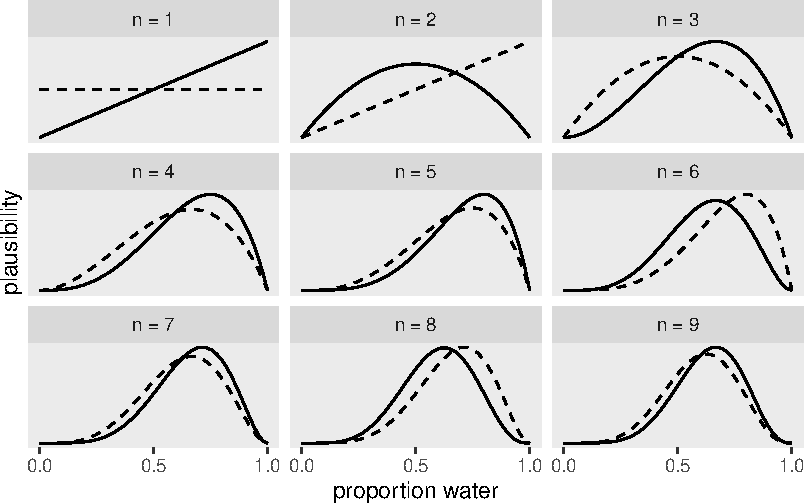
\includegraphics{02-small-and-large-worlds_files/figure-pdf/fig-bayesian-model-learning-1.pdf}

}

\caption{\label{fig-bayesian-model-learning}How a Bayesian model learns}

\end{figure}

\hypertarget{sec-annotation-1-expand-grid}{%
\paragraph{\texorpdfstring{Annotation (1):
\texttt{tidyr::expand\_grid()}}{Annotation (1): tidyr::expand\_grid()}}\label{sec-annotation-1-expand-grid}}

\texttt{tidyr::expand\_grid()} creates a tibble from all combinations of
inputs. Input are generalized vectors in contrast to
\texttt{tidyr::expand()} that generates all combination of variables as
well but needs as input a dataset. The range between 0 and 1 is divided
into 50 part and then it generates all combinations by varying all
columns from left to right. The first column is the slowest, the second
is faster and so on.). It generates 450 data points (50 * 9 trials).

\begin{Shaded}
\begin{Highlighting}[]
\InformationTok{\textasciigrave{}\textasciigrave{}\textasciigrave{}\{r\}}
\CommentTok{\#| label: bayesian{-}model{-}learning{-}anno1}

\CommentTok{\# starting data}
\NormalTok{tbl }\OtherTok{\textless{}{-}} \FunctionTok{tibble}\NormalTok{(}\AttributeTok{toss =} \FunctionTok{c}\NormalTok{(}\StringTok{"w"}\NormalTok{, }\StringTok{"l"}\NormalTok{, }\StringTok{"w"}\NormalTok{, }\StringTok{"w"}\NormalTok{, }\StringTok{"w"}\NormalTok{, }\StringTok{"l"}\NormalTok{, }\StringTok{"w"}\NormalTok{, }\StringTok{"l"}\NormalTok{, }\StringTok{"w"}\NormalTok{)) }\SpecialCharTok{|\textgreater{}} 
    \FunctionTok{mutate}\NormalTok{(}\AttributeTok{n\_trials  =} \DecValTok{1}\SpecialCharTok{:}\DecValTok{9}\NormalTok{, }\AttributeTok{n\_success =} \FunctionTok{cumsum}\NormalTok{(toss }\SpecialCharTok{==} \StringTok{"w"}\NormalTok{))}

\CommentTok{\# start of bayesian modeling}

\DocumentationTok{\#\#\# add code lines of annotation \textless{}1\textgreater{} \#\#\#\#\#\#\#\#\#\#\#\#\#\#\#\#\#\#\#\#\#\#\#\#\#\#\#\#\#\#\#\#\#\#\#\#\#\#\#\#\#}
\NormalTok{sequence\_length }\OtherTok{\textless{}{-}} \DecValTok{50}

\NormalTok{tbl }\SpecialCharTok{\%\textgreater{}\%} 
  \FunctionTok{expand\_grid}\NormalTok{(}\AttributeTok{p\_water =} \FunctionTok{seq}\NormalTok{(}\AttributeTok{from =} \DecValTok{0}\NormalTok{, }\AttributeTok{to =} \DecValTok{1}\NormalTok{, }
                            \AttributeTok{length.out =}\NormalTok{ sequence\_length))}
\InformationTok{\textasciigrave{}\textasciigrave{}\textasciigrave{}}
\end{Highlighting}
\end{Shaded}

\begin{verbatim}
#> # A tibble: 450 x 4
#>    toss  n_trials n_success p_water
#>    <chr>    <int>     <int>   <dbl>
#>  1 w            1         1  0     
#>  2 w            1         1  0.0204
#>  3 w            1         1  0.0408
#>  4 w            1         1  0.0612
#>  5 w            1         1  0.0816
#>  6 w            1         1  0.102 
#>  7 w            1         1  0.122 
#>  8 w            1         1  0.143 
#>  9 w            1         1  0.163 
#> 10 w            1         1  0.184 
#> # i 440 more rows
\end{verbatim}

\hypertarget{sec-annotation-2-group_by}{%
\paragraph{\texorpdfstring{Annotation (2):
\texttt{dplyr::group\_by()}}{Annotation (2): dplyr::group\_by()}}\label{sec-annotation-2-group_by}}

At first I did not understand the line \texttt{group\_by(p\_water)}. Why
has the data to be grouped when every row has a different value --- as I
have thought from a cursory inspection of the result? But it turned out
that after 100 records the parameter \texttt{p\_water} is repeating its
value.

\begin{tcolorbox}[enhanced jigsaw, colframe=quarto-callout-tip-color-frame, colback=white, toprule=.15mm, breakable, arc=.35mm, bottomtitle=1mm, colbacktitle=quarto-callout-tip-color!10!white, toptitle=1mm, titlerule=0mm, title=\textcolor{quarto-callout-tip-color}{\faLightbulb}\hspace{0.5em}{Special table format}, leftrule=.75mm, opacityback=0, rightrule=.15mm, opacitybacktitle=0.6, bottomrule=.15mm, left=2mm, coltitle=black]

For a better comparison (and for a later cross reference I will append
to the next code chunk a new column ID with line number and a table
format where one can scroll the long table with it 450 rows.

\end{tcolorbox}

\begin{Shaded}
\begin{Highlighting}[]
\InformationTok{\textasciigrave{}\textasciigrave{}\textasciigrave{}\{r\}}
\CommentTok{\#| label: tbl{-}bayesian{-}model{-}learning{-}anno2{-}1}
\CommentTok{\#| tbl{-}cap: "Bayesian Updating: Lagged with groupping"}

\CommentTok{\# starting data}
\NormalTok{tbl1 }\OtherTok{\textless{}{-}} \FunctionTok{tibble}\NormalTok{(}\AttributeTok{toss =} \FunctionTok{c}\NormalTok{(}\StringTok{"w"}\NormalTok{, }\StringTok{"l"}\NormalTok{, }\StringTok{"w"}\NormalTok{, }\StringTok{"w"}\NormalTok{, }\StringTok{"w"}\NormalTok{, }\StringTok{"l"}\NormalTok{, }\StringTok{"w"}\NormalTok{, }\StringTok{"l"}\NormalTok{, }\StringTok{"w"}\NormalTok{)) }\SpecialCharTok{|\textgreater{}}
    \FunctionTok{mutate}\NormalTok{(}\AttributeTok{n\_trials  =} \DecValTok{1}\SpecialCharTok{:}\DecValTok{9}\NormalTok{, }\AttributeTok{n\_success =} \FunctionTok{cumsum}\NormalTok{(toss }\SpecialCharTok{==} \StringTok{"w"}\NormalTok{))}

\CommentTok{\# start of bayesian modeling with grouping (as in the original)}
\NormalTok{sequence\_length }\OtherTok{\textless{}{-}} \DecValTok{50}

\NormalTok{tbl1 }\OtherTok{\textless{}{-}}\NormalTok{ tbl }\SpecialCharTok{\%\textgreater{}\%} 
  \FunctionTok{expand\_grid}\NormalTok{(}\AttributeTok{p\_water =} \FunctionTok{seq}\NormalTok{(}\AttributeTok{from =} \DecValTok{0}\NormalTok{, }\AttributeTok{to =} \DecValTok{1}\NormalTok{, }
                            \AttributeTok{length.out =}\NormalTok{ sequence\_length)) }\SpecialCharTok{\%\textgreater{}\%} 
    
  \DocumentationTok{\#\#\#\# add code lines to show effect of annoation \textless{}2\textgreater{} \#\#\#\#\#\#\#\#\#\#\#\#\#\#\#\#\#\#\#\#\#\#}
  \FunctionTok{group\_by}\NormalTok{(p\_water) }\SpecialCharTok{\%\textgreater{}\%} 
  \FunctionTok{mutate}\NormalTok{(}\AttributeTok{lagged\_n\_trials  =} \FunctionTok{lag}\NormalTok{(n\_trials, }\AttributeTok{default =} \DecValTok{1}\NormalTok{),}
         \AttributeTok{lagged\_n\_success =} \FunctionTok{lag}\NormalTok{(n\_success, }\AttributeTok{default =} \DecValTok{1}\NormalTok{)) }\SpecialCharTok{\%\textgreater{}\%} 
  \FunctionTok{ungroup}\NormalTok{() }\SpecialCharTok{|\textgreater{}} 
    

  \CommentTok{\# add new column ID with row numbers }
  \CommentTok{\# and relocate it to be the first column}
  \FunctionTok{mutate}\NormalTok{(}\AttributeTok{ID =} \FunctionTok{row\_number}\NormalTok{()) }\SpecialCharTok{|\textgreater{}} 
  \FunctionTok{relocate}\NormalTok{(ID, }\AttributeTok{.before =}\NormalTok{ toss) }\SpecialCharTok{|\textgreater{}} 

 \CommentTok{\# provide a different format and a scroll box for the table}
\NormalTok{  kableExtra}\SpecialCharTok{::}\FunctionTok{kbl}\NormalTok{() }\SpecialCharTok{\%\textgreater{}\%}
\NormalTok{  kableExtra}\SpecialCharTok{::}\FunctionTok{kable\_classic}\NormalTok{() }\SpecialCharTok{\%\textgreater{}\%}
\NormalTok{  kableExtra}\SpecialCharTok{::}\FunctionTok{scroll\_box}\NormalTok{(}\AttributeTok{height =} \StringTok{"600px"}\NormalTok{)}
\NormalTok{tbl1}
\InformationTok{\textasciigrave{}\textasciigrave{}\textasciigrave{}}
\end{Highlighting}
\end{Shaded}

\hypertarget{tbl-bayesian-model-learning-anno2-1}{}
\begin{table}
\caption{\label{tbl-bayesian-model-learning-anno2-1}Bayesian Updating: Lagged with groupping }\tabularnewline

\centering
\begin{tabular}[t]{r|l|r|r|r|r|r}
\hline
ID & toss & n\_trials & n\_success & p\_water & lagged\_n\_trials & lagged\_n\_success\\
\hline
1 & w & 1 & 1 & 0.0000000 & 1 & 1\\
\hline
2 & w & 1 & 1 & 0.0204082 & 1 & 1\\
\hline
3 & w & 1 & 1 & 0.0408163 & 1 & 1\\
\hline
4 & w & 1 & 1 & 0.0612245 & 1 & 1\\
\hline
5 & w & 1 & 1 & 0.0816327 & 1 & 1\\
\hline
6 & w & 1 & 1 & 0.1020408 & 1 & 1\\
\hline
7 & w & 1 & 1 & 0.1224490 & 1 & 1\\
\hline
8 & w & 1 & 1 & 0.1428571 & 1 & 1\\
\hline
9 & w & 1 & 1 & 0.1632653 & 1 & 1\\
\hline
10 & w & 1 & 1 & 0.1836735 & 1 & 1\\
\hline
11 & w & 1 & 1 & 0.2040816 & 1 & 1\\
\hline
12 & w & 1 & 1 & 0.2244898 & 1 & 1\\
\hline
13 & w & 1 & 1 & 0.2448980 & 1 & 1\\
\hline
14 & w & 1 & 1 & 0.2653061 & 1 & 1\\
\hline
15 & w & 1 & 1 & 0.2857143 & 1 & 1\\
\hline
16 & w & 1 & 1 & 0.3061224 & 1 & 1\\
\hline
17 & w & 1 & 1 & 0.3265306 & 1 & 1\\
\hline
18 & w & 1 & 1 & 0.3469388 & 1 & 1\\
\hline
19 & w & 1 & 1 & 0.3673469 & 1 & 1\\
\hline
20 & w & 1 & 1 & 0.3877551 & 1 & 1\\
\hline
21 & w & 1 & 1 & 0.4081633 & 1 & 1\\
\hline
22 & w & 1 & 1 & 0.4285714 & 1 & 1\\
\hline
23 & w & 1 & 1 & 0.4489796 & 1 & 1\\
\hline
24 & w & 1 & 1 & 0.4693878 & 1 & 1\\
\hline
25 & w & 1 & 1 & 0.4897959 & 1 & 1\\
\hline
26 & w & 1 & 1 & 0.5102041 & 1 & 1\\
\hline
27 & w & 1 & 1 & 0.5306122 & 1 & 1\\
\hline
28 & w & 1 & 1 & 0.5510204 & 1 & 1\\
\hline
29 & w & 1 & 1 & 0.5714286 & 1 & 1\\
\hline
30 & w & 1 & 1 & 0.5918367 & 1 & 1\\
\hline
31 & w & 1 & 1 & 0.6122449 & 1 & 1\\
\hline
32 & w & 1 & 1 & 0.6326531 & 1 & 1\\
\hline
33 & w & 1 & 1 & 0.6530612 & 1 & 1\\
\hline
34 & w & 1 & 1 & 0.6734694 & 1 & 1\\
\hline
35 & w & 1 & 1 & 0.6938776 & 1 & 1\\
\hline
36 & w & 1 & 1 & 0.7142857 & 1 & 1\\
\hline
37 & w & 1 & 1 & 0.7346939 & 1 & 1\\
\hline
38 & w & 1 & 1 & 0.7551020 & 1 & 1\\
\hline
39 & w & 1 & 1 & 0.7755102 & 1 & 1\\
\hline
40 & w & 1 & 1 & 0.7959184 & 1 & 1\\
\hline
41 & w & 1 & 1 & 0.8163265 & 1 & 1\\
\hline
42 & w & 1 & 1 & 0.8367347 & 1 & 1\\
\hline
43 & w & 1 & 1 & 0.8571429 & 1 & 1\\
\hline
44 & w & 1 & 1 & 0.8775510 & 1 & 1\\
\hline
45 & w & 1 & 1 & 0.8979592 & 1 & 1\\
\hline
46 & w & 1 & 1 & 0.9183673 & 1 & 1\\
\hline
47 & w & 1 & 1 & 0.9387755 & 1 & 1\\
\hline
48 & w & 1 & 1 & 0.9591837 & 1 & 1\\
\hline
49 & w & 1 & 1 & 0.9795918 & 1 & 1\\
\hline
50 & w & 1 & 1 & 1.0000000 & 1 & 1\\
\hline
51 & l & 2 & 1 & 0.0000000 & 1 & 1\\
\hline
52 & l & 2 & 1 & 0.0204082 & 1 & 1\\
\hline
53 & l & 2 & 1 & 0.0408163 & 1 & 1\\
\hline
54 & l & 2 & 1 & 0.0612245 & 1 & 1\\
\hline
55 & l & 2 & 1 & 0.0816327 & 1 & 1\\
\hline
56 & l & 2 & 1 & 0.1020408 & 1 & 1\\
\hline
57 & l & 2 & 1 & 0.1224490 & 1 & 1\\
\hline
58 & l & 2 & 1 & 0.1428571 & 1 & 1\\
\hline
59 & l & 2 & 1 & 0.1632653 & 1 & 1\\
\hline
60 & l & 2 & 1 & 0.1836735 & 1 & 1\\
\hline
61 & l & 2 & 1 & 0.2040816 & 1 & 1\\
\hline
62 & l & 2 & 1 & 0.2244898 & 1 & 1\\
\hline
63 & l & 2 & 1 & 0.2448980 & 1 & 1\\
\hline
64 & l & 2 & 1 & 0.2653061 & 1 & 1\\
\hline
65 & l & 2 & 1 & 0.2857143 & 1 & 1\\
\hline
66 & l & 2 & 1 & 0.3061224 & 1 & 1\\
\hline
67 & l & 2 & 1 & 0.3265306 & 1 & 1\\
\hline
68 & l & 2 & 1 & 0.3469388 & 1 & 1\\
\hline
69 & l & 2 & 1 & 0.3673469 & 1 & 1\\
\hline
70 & l & 2 & 1 & 0.3877551 & 1 & 1\\
\hline
71 & l & 2 & 1 & 0.4081633 & 1 & 1\\
\hline
72 & l & 2 & 1 & 0.4285714 & 1 & 1\\
\hline
73 & l & 2 & 1 & 0.4489796 & 1 & 1\\
\hline
74 & l & 2 & 1 & 0.4693878 & 1 & 1\\
\hline
75 & l & 2 & 1 & 0.4897959 & 1 & 1\\
\hline
76 & l & 2 & 1 & 0.5102041 & 1 & 1\\
\hline
77 & l & 2 & 1 & 0.5306122 & 1 & 1\\
\hline
78 & l & 2 & 1 & 0.5510204 & 1 & 1\\
\hline
79 & l & 2 & 1 & 0.5714286 & 1 & 1\\
\hline
80 & l & 2 & 1 & 0.5918367 & 1 & 1\\
\hline
81 & l & 2 & 1 & 0.6122449 & 1 & 1\\
\hline
82 & l & 2 & 1 & 0.6326531 & 1 & 1\\
\hline
83 & l & 2 & 1 & 0.6530612 & 1 & 1\\
\hline
84 & l & 2 & 1 & 0.6734694 & 1 & 1\\
\hline
85 & l & 2 & 1 & 0.6938776 & 1 & 1\\
\hline
86 & l & 2 & 1 & 0.7142857 & 1 & 1\\
\hline
87 & l & 2 & 1 & 0.7346939 & 1 & 1\\
\hline
88 & l & 2 & 1 & 0.7551020 & 1 & 1\\
\hline
89 & l & 2 & 1 & 0.7755102 & 1 & 1\\
\hline
90 & l & 2 & 1 & 0.7959184 & 1 & 1\\
\hline
91 & l & 2 & 1 & 0.8163265 & 1 & 1\\
\hline
92 & l & 2 & 1 & 0.8367347 & 1 & 1\\
\hline
93 & l & 2 & 1 & 0.8571429 & 1 & 1\\
\hline
94 & l & 2 & 1 & 0.8775510 & 1 & 1\\
\hline
95 & l & 2 & 1 & 0.8979592 & 1 & 1\\
\hline
96 & l & 2 & 1 & 0.9183673 & 1 & 1\\
\hline
97 & l & 2 & 1 & 0.9387755 & 1 & 1\\
\hline
98 & l & 2 & 1 & 0.9591837 & 1 & 1\\
\hline
99 & l & 2 & 1 & 0.9795918 & 1 & 1\\
\hline
100 & l & 2 & 1 & 1.0000000 & 1 & 1\\
\hline
101 & w & 3 & 2 & 0.0000000 & 2 & 1\\
\hline
102 & w & 3 & 2 & 0.0204082 & 2 & 1\\
\hline
103 & w & 3 & 2 & 0.0408163 & 2 & 1\\
\hline
104 & w & 3 & 2 & 0.0612245 & 2 & 1\\
\hline
105 & w & 3 & 2 & 0.0816327 & 2 & 1\\
\hline
106 & w & 3 & 2 & 0.1020408 & 2 & 1\\
\hline
107 & w & 3 & 2 & 0.1224490 & 2 & 1\\
\hline
108 & w & 3 & 2 & 0.1428571 & 2 & 1\\
\hline
109 & w & 3 & 2 & 0.1632653 & 2 & 1\\
\hline
110 & w & 3 & 2 & 0.1836735 & 2 & 1\\
\hline
111 & w & 3 & 2 & 0.2040816 & 2 & 1\\
\hline
112 & w & 3 & 2 & 0.2244898 & 2 & 1\\
\hline
113 & w & 3 & 2 & 0.2448980 & 2 & 1\\
\hline
114 & w & 3 & 2 & 0.2653061 & 2 & 1\\
\hline
115 & w & 3 & 2 & 0.2857143 & 2 & 1\\
\hline
116 & w & 3 & 2 & 0.3061224 & 2 & 1\\
\hline
117 & w & 3 & 2 & 0.3265306 & 2 & 1\\
\hline
118 & w & 3 & 2 & 0.3469388 & 2 & 1\\
\hline
119 & w & 3 & 2 & 0.3673469 & 2 & 1\\
\hline
120 & w & 3 & 2 & 0.3877551 & 2 & 1\\
\hline
121 & w & 3 & 2 & 0.4081633 & 2 & 1\\
\hline
122 & w & 3 & 2 & 0.4285714 & 2 & 1\\
\hline
123 & w & 3 & 2 & 0.4489796 & 2 & 1\\
\hline
124 & w & 3 & 2 & 0.4693878 & 2 & 1\\
\hline
125 & w & 3 & 2 & 0.4897959 & 2 & 1\\
\hline
126 & w & 3 & 2 & 0.5102041 & 2 & 1\\
\hline
127 & w & 3 & 2 & 0.5306122 & 2 & 1\\
\hline
128 & w & 3 & 2 & 0.5510204 & 2 & 1\\
\hline
129 & w & 3 & 2 & 0.5714286 & 2 & 1\\
\hline
130 & w & 3 & 2 & 0.5918367 & 2 & 1\\
\hline
131 & w & 3 & 2 & 0.6122449 & 2 & 1\\
\hline
132 & w & 3 & 2 & 0.6326531 & 2 & 1\\
\hline
133 & w & 3 & 2 & 0.6530612 & 2 & 1\\
\hline
134 & w & 3 & 2 & 0.6734694 & 2 & 1\\
\hline
135 & w & 3 & 2 & 0.6938776 & 2 & 1\\
\hline
136 & w & 3 & 2 & 0.7142857 & 2 & 1\\
\hline
137 & w & 3 & 2 & 0.7346939 & 2 & 1\\
\hline
138 & w & 3 & 2 & 0.7551020 & 2 & 1\\
\hline
139 & w & 3 & 2 & 0.7755102 & 2 & 1\\
\hline
140 & w & 3 & 2 & 0.7959184 & 2 & 1\\
\hline
141 & w & 3 & 2 & 0.8163265 & 2 & 1\\
\hline
142 & w & 3 & 2 & 0.8367347 & 2 & 1\\
\hline
143 & w & 3 & 2 & 0.8571429 & 2 & 1\\
\hline
144 & w & 3 & 2 & 0.8775510 & 2 & 1\\
\hline
145 & w & 3 & 2 & 0.8979592 & 2 & 1\\
\hline
146 & w & 3 & 2 & 0.9183673 & 2 & 1\\
\hline
147 & w & 3 & 2 & 0.9387755 & 2 & 1\\
\hline
148 & w & 3 & 2 & 0.9591837 & 2 & 1\\
\hline
149 & w & 3 & 2 & 0.9795918 & 2 & 1\\
\hline
150 & w & 3 & 2 & 1.0000000 & 2 & 1\\
\hline
151 & w & 4 & 3 & 0.0000000 & 3 & 2\\
\hline
152 & w & 4 & 3 & 0.0204082 & 3 & 2\\
\hline
153 & w & 4 & 3 & 0.0408163 & 3 & 2\\
\hline
154 & w & 4 & 3 & 0.0612245 & 3 & 2\\
\hline
155 & w & 4 & 3 & 0.0816327 & 3 & 2\\
\hline
156 & w & 4 & 3 & 0.1020408 & 3 & 2\\
\hline
157 & w & 4 & 3 & 0.1224490 & 3 & 2\\
\hline
158 & w & 4 & 3 & 0.1428571 & 3 & 2\\
\hline
159 & w & 4 & 3 & 0.1632653 & 3 & 2\\
\hline
160 & w & 4 & 3 & 0.1836735 & 3 & 2\\
\hline
161 & w & 4 & 3 & 0.2040816 & 3 & 2\\
\hline
162 & w & 4 & 3 & 0.2244898 & 3 & 2\\
\hline
163 & w & 4 & 3 & 0.2448980 & 3 & 2\\
\hline
164 & w & 4 & 3 & 0.2653061 & 3 & 2\\
\hline
165 & w & 4 & 3 & 0.2857143 & 3 & 2\\
\hline
166 & w & 4 & 3 & 0.3061224 & 3 & 2\\
\hline
167 & w & 4 & 3 & 0.3265306 & 3 & 2\\
\hline
168 & w & 4 & 3 & 0.3469388 & 3 & 2\\
\hline
169 & w & 4 & 3 & 0.3673469 & 3 & 2\\
\hline
170 & w & 4 & 3 & 0.3877551 & 3 & 2\\
\hline
171 & w & 4 & 3 & 0.4081633 & 3 & 2\\
\hline
172 & w & 4 & 3 & 0.4285714 & 3 & 2\\
\hline
173 & w & 4 & 3 & 0.4489796 & 3 & 2\\
\hline
174 & w & 4 & 3 & 0.4693878 & 3 & 2\\
\hline
175 & w & 4 & 3 & 0.4897959 & 3 & 2\\
\hline
176 & w & 4 & 3 & 0.5102041 & 3 & 2\\
\hline
177 & w & 4 & 3 & 0.5306122 & 3 & 2\\
\hline
178 & w & 4 & 3 & 0.5510204 & 3 & 2\\
\hline
179 & w & 4 & 3 & 0.5714286 & 3 & 2\\
\hline
180 & w & 4 & 3 & 0.5918367 & 3 & 2\\
\hline
181 & w & 4 & 3 & 0.6122449 & 3 & 2\\
\hline
182 & w & 4 & 3 & 0.6326531 & 3 & 2\\
\hline
183 & w & 4 & 3 & 0.6530612 & 3 & 2\\
\hline
184 & w & 4 & 3 & 0.6734694 & 3 & 2\\
\hline
185 & w & 4 & 3 & 0.6938776 & 3 & 2\\
\hline
186 & w & 4 & 3 & 0.7142857 & 3 & 2\\
\hline
187 & w & 4 & 3 & 0.7346939 & 3 & 2\\
\hline
188 & w & 4 & 3 & 0.7551020 & 3 & 2\\
\hline
189 & w & 4 & 3 & 0.7755102 & 3 & 2\\
\hline
190 & w & 4 & 3 & 0.7959184 & 3 & 2\\
\hline
191 & w & 4 & 3 & 0.8163265 & 3 & 2\\
\hline
192 & w & 4 & 3 & 0.8367347 & 3 & 2\\
\hline
193 & w & 4 & 3 & 0.8571429 & 3 & 2\\
\hline
194 & w & 4 & 3 & 0.8775510 & 3 & 2\\
\hline
195 & w & 4 & 3 & 0.8979592 & 3 & 2\\
\hline
196 & w & 4 & 3 & 0.9183673 & 3 & 2\\
\hline
197 & w & 4 & 3 & 0.9387755 & 3 & 2\\
\hline
198 & w & 4 & 3 & 0.9591837 & 3 & 2\\
\hline
199 & w & 4 & 3 & 0.9795918 & 3 & 2\\
\hline
200 & w & 4 & 3 & 1.0000000 & 3 & 2\\
\hline
201 & w & 5 & 4 & 0.0000000 & 4 & 3\\
\hline
202 & w & 5 & 4 & 0.0204082 & 4 & 3\\
\hline
203 & w & 5 & 4 & 0.0408163 & 4 & 3\\
\hline
204 & w & 5 & 4 & 0.0612245 & 4 & 3\\
\hline
205 & w & 5 & 4 & 0.0816327 & 4 & 3\\
\hline
206 & w & 5 & 4 & 0.1020408 & 4 & 3\\
\hline
207 & w & 5 & 4 & 0.1224490 & 4 & 3\\
\hline
208 & w & 5 & 4 & 0.1428571 & 4 & 3\\
\hline
209 & w & 5 & 4 & 0.1632653 & 4 & 3\\
\hline
210 & w & 5 & 4 & 0.1836735 & 4 & 3\\
\hline
211 & w & 5 & 4 & 0.2040816 & 4 & 3\\
\hline
212 & w & 5 & 4 & 0.2244898 & 4 & 3\\
\hline
213 & w & 5 & 4 & 0.2448980 & 4 & 3\\
\hline
214 & w & 5 & 4 & 0.2653061 & 4 & 3\\
\hline
215 & w & 5 & 4 & 0.2857143 & 4 & 3\\
\hline
216 & w & 5 & 4 & 0.3061224 & 4 & 3\\
\hline
217 & w & 5 & 4 & 0.3265306 & 4 & 3\\
\hline
218 & w & 5 & 4 & 0.3469388 & 4 & 3\\
\hline
219 & w & 5 & 4 & 0.3673469 & 4 & 3\\
\hline
220 & w & 5 & 4 & 0.3877551 & 4 & 3\\
\hline
221 & w & 5 & 4 & 0.4081633 & 4 & 3\\
\hline
222 & w & 5 & 4 & 0.4285714 & 4 & 3\\
\hline
223 & w & 5 & 4 & 0.4489796 & 4 & 3\\
\hline
224 & w & 5 & 4 & 0.4693878 & 4 & 3\\
\hline
225 & w & 5 & 4 & 0.4897959 & 4 & 3\\
\hline
226 & w & 5 & 4 & 0.5102041 & 4 & 3\\
\hline
227 & w & 5 & 4 & 0.5306122 & 4 & 3\\
\hline
228 & w & 5 & 4 & 0.5510204 & 4 & 3\\
\hline
229 & w & 5 & 4 & 0.5714286 & 4 & 3\\
\hline
230 & w & 5 & 4 & 0.5918367 & 4 & 3\\
\hline
231 & w & 5 & 4 & 0.6122449 & 4 & 3\\
\hline
232 & w & 5 & 4 & 0.6326531 & 4 & 3\\
\hline
233 & w & 5 & 4 & 0.6530612 & 4 & 3\\
\hline
234 & w & 5 & 4 & 0.6734694 & 4 & 3\\
\hline
235 & w & 5 & 4 & 0.6938776 & 4 & 3\\
\hline
236 & w & 5 & 4 & 0.7142857 & 4 & 3\\
\hline
237 & w & 5 & 4 & 0.7346939 & 4 & 3\\
\hline
238 & w & 5 & 4 & 0.7551020 & 4 & 3\\
\hline
239 & w & 5 & 4 & 0.7755102 & 4 & 3\\
\hline
240 & w & 5 & 4 & 0.7959184 & 4 & 3\\
\hline
241 & w & 5 & 4 & 0.8163265 & 4 & 3\\
\hline
242 & w & 5 & 4 & 0.8367347 & 4 & 3\\
\hline
243 & w & 5 & 4 & 0.8571429 & 4 & 3\\
\hline
244 & w & 5 & 4 & 0.8775510 & 4 & 3\\
\hline
245 & w & 5 & 4 & 0.8979592 & 4 & 3\\
\hline
246 & w & 5 & 4 & 0.9183673 & 4 & 3\\
\hline
247 & w & 5 & 4 & 0.9387755 & 4 & 3\\
\hline
248 & w & 5 & 4 & 0.9591837 & 4 & 3\\
\hline
249 & w & 5 & 4 & 0.9795918 & 4 & 3\\
\hline
250 & w & 5 & 4 & 1.0000000 & 4 & 3\\
\hline
251 & l & 6 & 4 & 0.0000000 & 5 & 4\\
\hline
252 & l & 6 & 4 & 0.0204082 & 5 & 4\\
\hline
253 & l & 6 & 4 & 0.0408163 & 5 & 4\\
\hline
254 & l & 6 & 4 & 0.0612245 & 5 & 4\\
\hline
255 & l & 6 & 4 & 0.0816327 & 5 & 4\\
\hline
256 & l & 6 & 4 & 0.1020408 & 5 & 4\\
\hline
257 & l & 6 & 4 & 0.1224490 & 5 & 4\\
\hline
258 & l & 6 & 4 & 0.1428571 & 5 & 4\\
\hline
259 & l & 6 & 4 & 0.1632653 & 5 & 4\\
\hline
260 & l & 6 & 4 & 0.1836735 & 5 & 4\\
\hline
261 & l & 6 & 4 & 0.2040816 & 5 & 4\\
\hline
262 & l & 6 & 4 & 0.2244898 & 5 & 4\\
\hline
263 & l & 6 & 4 & 0.2448980 & 5 & 4\\
\hline
264 & l & 6 & 4 & 0.2653061 & 5 & 4\\
\hline
265 & l & 6 & 4 & 0.2857143 & 5 & 4\\
\hline
266 & l & 6 & 4 & 0.3061224 & 5 & 4\\
\hline
267 & l & 6 & 4 & 0.3265306 & 5 & 4\\
\hline
268 & l & 6 & 4 & 0.3469388 & 5 & 4\\
\hline
269 & l & 6 & 4 & 0.3673469 & 5 & 4\\
\hline
270 & l & 6 & 4 & 0.3877551 & 5 & 4\\
\hline
271 & l & 6 & 4 & 0.4081633 & 5 & 4\\
\hline
272 & l & 6 & 4 & 0.4285714 & 5 & 4\\
\hline
273 & l & 6 & 4 & 0.4489796 & 5 & 4\\
\hline
274 & l & 6 & 4 & 0.4693878 & 5 & 4\\
\hline
275 & l & 6 & 4 & 0.4897959 & 5 & 4\\
\hline
276 & l & 6 & 4 & 0.5102041 & 5 & 4\\
\hline
277 & l & 6 & 4 & 0.5306122 & 5 & 4\\
\hline
278 & l & 6 & 4 & 0.5510204 & 5 & 4\\
\hline
279 & l & 6 & 4 & 0.5714286 & 5 & 4\\
\hline
280 & l & 6 & 4 & 0.5918367 & 5 & 4\\
\hline
281 & l & 6 & 4 & 0.6122449 & 5 & 4\\
\hline
282 & l & 6 & 4 & 0.6326531 & 5 & 4\\
\hline
283 & l & 6 & 4 & 0.6530612 & 5 & 4\\
\hline
284 & l & 6 & 4 & 0.6734694 & 5 & 4\\
\hline
285 & l & 6 & 4 & 0.6938776 & 5 & 4\\
\hline
286 & l & 6 & 4 & 0.7142857 & 5 & 4\\
\hline
287 & l & 6 & 4 & 0.7346939 & 5 & 4\\
\hline
288 & l & 6 & 4 & 0.7551020 & 5 & 4\\
\hline
289 & l & 6 & 4 & 0.7755102 & 5 & 4\\
\hline
290 & l & 6 & 4 & 0.7959184 & 5 & 4\\
\hline
291 & l & 6 & 4 & 0.8163265 & 5 & 4\\
\hline
292 & l & 6 & 4 & 0.8367347 & 5 & 4\\
\hline
293 & l & 6 & 4 & 0.8571429 & 5 & 4\\
\hline
294 & l & 6 & 4 & 0.8775510 & 5 & 4\\
\hline
295 & l & 6 & 4 & 0.8979592 & 5 & 4\\
\hline
296 & l & 6 & 4 & 0.9183673 & 5 & 4\\
\hline
297 & l & 6 & 4 & 0.9387755 & 5 & 4\\
\hline
298 & l & 6 & 4 & 0.9591837 & 5 & 4\\
\hline
299 & l & 6 & 4 & 0.9795918 & 5 & 4\\
\hline
300 & l & 6 & 4 & 1.0000000 & 5 & 4\\
\hline
301 & w & 7 & 5 & 0.0000000 & 6 & 4\\
\hline
302 & w & 7 & 5 & 0.0204082 & 6 & 4\\
\hline
303 & w & 7 & 5 & 0.0408163 & 6 & 4\\
\hline
304 & w & 7 & 5 & 0.0612245 & 6 & 4\\
\hline
305 & w & 7 & 5 & 0.0816327 & 6 & 4\\
\hline
306 & w & 7 & 5 & 0.1020408 & 6 & 4\\
\hline
307 & w & 7 & 5 & 0.1224490 & 6 & 4\\
\hline
308 & w & 7 & 5 & 0.1428571 & 6 & 4\\
\hline
309 & w & 7 & 5 & 0.1632653 & 6 & 4\\
\hline
310 & w & 7 & 5 & 0.1836735 & 6 & 4\\
\hline
311 & w & 7 & 5 & 0.2040816 & 6 & 4\\
\hline
312 & w & 7 & 5 & 0.2244898 & 6 & 4\\
\hline
313 & w & 7 & 5 & 0.2448980 & 6 & 4\\
\hline
314 & w & 7 & 5 & 0.2653061 & 6 & 4\\
\hline
315 & w & 7 & 5 & 0.2857143 & 6 & 4\\
\hline
316 & w & 7 & 5 & 0.3061224 & 6 & 4\\
\hline
317 & w & 7 & 5 & 0.3265306 & 6 & 4\\
\hline
318 & w & 7 & 5 & 0.3469388 & 6 & 4\\
\hline
319 & w & 7 & 5 & 0.3673469 & 6 & 4\\
\hline
320 & w & 7 & 5 & 0.3877551 & 6 & 4\\
\hline
321 & w & 7 & 5 & 0.4081633 & 6 & 4\\
\hline
322 & w & 7 & 5 & 0.4285714 & 6 & 4\\
\hline
323 & w & 7 & 5 & 0.4489796 & 6 & 4\\
\hline
324 & w & 7 & 5 & 0.4693878 & 6 & 4\\
\hline
325 & w & 7 & 5 & 0.4897959 & 6 & 4\\
\hline
326 & w & 7 & 5 & 0.5102041 & 6 & 4\\
\hline
327 & w & 7 & 5 & 0.5306122 & 6 & 4\\
\hline
328 & w & 7 & 5 & 0.5510204 & 6 & 4\\
\hline
329 & w & 7 & 5 & 0.5714286 & 6 & 4\\
\hline
330 & w & 7 & 5 & 0.5918367 & 6 & 4\\
\hline
331 & w & 7 & 5 & 0.6122449 & 6 & 4\\
\hline
332 & w & 7 & 5 & 0.6326531 & 6 & 4\\
\hline
333 & w & 7 & 5 & 0.6530612 & 6 & 4\\
\hline
334 & w & 7 & 5 & 0.6734694 & 6 & 4\\
\hline
335 & w & 7 & 5 & 0.6938776 & 6 & 4\\
\hline
336 & w & 7 & 5 & 0.7142857 & 6 & 4\\
\hline
337 & w & 7 & 5 & 0.7346939 & 6 & 4\\
\hline
338 & w & 7 & 5 & 0.7551020 & 6 & 4\\
\hline
339 & w & 7 & 5 & 0.7755102 & 6 & 4\\
\hline
340 & w & 7 & 5 & 0.7959184 & 6 & 4\\
\hline
341 & w & 7 & 5 & 0.8163265 & 6 & 4\\
\hline
342 & w & 7 & 5 & 0.8367347 & 6 & 4\\
\hline
343 & w & 7 & 5 & 0.8571429 & 6 & 4\\
\hline
344 & w & 7 & 5 & 0.8775510 & 6 & 4\\
\hline
345 & w & 7 & 5 & 0.8979592 & 6 & 4\\
\hline
346 & w & 7 & 5 & 0.9183673 & 6 & 4\\
\hline
347 & w & 7 & 5 & 0.9387755 & 6 & 4\\
\hline
348 & w & 7 & 5 & 0.9591837 & 6 & 4\\
\hline
349 & w & 7 & 5 & 0.9795918 & 6 & 4\\
\hline
350 & w & 7 & 5 & 1.0000000 & 6 & 4\\
\hline
351 & l & 8 & 5 & 0.0000000 & 7 & 5\\
\hline
352 & l & 8 & 5 & 0.0204082 & 7 & 5\\
\hline
353 & l & 8 & 5 & 0.0408163 & 7 & 5\\
\hline
354 & l & 8 & 5 & 0.0612245 & 7 & 5\\
\hline
355 & l & 8 & 5 & 0.0816327 & 7 & 5\\
\hline
356 & l & 8 & 5 & 0.1020408 & 7 & 5\\
\hline
357 & l & 8 & 5 & 0.1224490 & 7 & 5\\
\hline
358 & l & 8 & 5 & 0.1428571 & 7 & 5\\
\hline
359 & l & 8 & 5 & 0.1632653 & 7 & 5\\
\hline
360 & l & 8 & 5 & 0.1836735 & 7 & 5\\
\hline
361 & l & 8 & 5 & 0.2040816 & 7 & 5\\
\hline
362 & l & 8 & 5 & 0.2244898 & 7 & 5\\
\hline
363 & l & 8 & 5 & 0.2448980 & 7 & 5\\
\hline
364 & l & 8 & 5 & 0.2653061 & 7 & 5\\
\hline
365 & l & 8 & 5 & 0.2857143 & 7 & 5\\
\hline
366 & l & 8 & 5 & 0.3061224 & 7 & 5\\
\hline
367 & l & 8 & 5 & 0.3265306 & 7 & 5\\
\hline
368 & l & 8 & 5 & 0.3469388 & 7 & 5\\
\hline
369 & l & 8 & 5 & 0.3673469 & 7 & 5\\
\hline
370 & l & 8 & 5 & 0.3877551 & 7 & 5\\
\hline
371 & l & 8 & 5 & 0.4081633 & 7 & 5\\
\hline
372 & l & 8 & 5 & 0.4285714 & 7 & 5\\
\hline
373 & l & 8 & 5 & 0.4489796 & 7 & 5\\
\hline
374 & l & 8 & 5 & 0.4693878 & 7 & 5\\
\hline
375 & l & 8 & 5 & 0.4897959 & 7 & 5\\
\hline
376 & l & 8 & 5 & 0.5102041 & 7 & 5\\
\hline
377 & l & 8 & 5 & 0.5306122 & 7 & 5\\
\hline
378 & l & 8 & 5 & 0.5510204 & 7 & 5\\
\hline
379 & l & 8 & 5 & 0.5714286 & 7 & 5\\
\hline
380 & l & 8 & 5 & 0.5918367 & 7 & 5\\
\hline
381 & l & 8 & 5 & 0.6122449 & 7 & 5\\
\hline
382 & l & 8 & 5 & 0.6326531 & 7 & 5\\
\hline
383 & l & 8 & 5 & 0.6530612 & 7 & 5\\
\hline
384 & l & 8 & 5 & 0.6734694 & 7 & 5\\
\hline
385 & l & 8 & 5 & 0.6938776 & 7 & 5\\
\hline
386 & l & 8 & 5 & 0.7142857 & 7 & 5\\
\hline
387 & l & 8 & 5 & 0.7346939 & 7 & 5\\
\hline
388 & l & 8 & 5 & 0.7551020 & 7 & 5\\
\hline
389 & l & 8 & 5 & 0.7755102 & 7 & 5\\
\hline
390 & l & 8 & 5 & 0.7959184 & 7 & 5\\
\hline
391 & l & 8 & 5 & 0.8163265 & 7 & 5\\
\hline
392 & l & 8 & 5 & 0.8367347 & 7 & 5\\
\hline
393 & l & 8 & 5 & 0.8571429 & 7 & 5\\
\hline
394 & l & 8 & 5 & 0.8775510 & 7 & 5\\
\hline
395 & l & 8 & 5 & 0.8979592 & 7 & 5\\
\hline
396 & l & 8 & 5 & 0.9183673 & 7 & 5\\
\hline
397 & l & 8 & 5 & 0.9387755 & 7 & 5\\
\hline
398 & l & 8 & 5 & 0.9591837 & 7 & 5\\
\hline
399 & l & 8 & 5 & 0.9795918 & 7 & 5\\
\hline
400 & l & 8 & 5 & 1.0000000 & 7 & 5\\
\hline
401 & w & 9 & 6 & 0.0000000 & 8 & 5\\
\hline
402 & w & 9 & 6 & 0.0204082 & 8 & 5\\
\hline
403 & w & 9 & 6 & 0.0408163 & 8 & 5\\
\hline
404 & w & 9 & 6 & 0.0612245 & 8 & 5\\
\hline
405 & w & 9 & 6 & 0.0816327 & 8 & 5\\
\hline
406 & w & 9 & 6 & 0.1020408 & 8 & 5\\
\hline
407 & w & 9 & 6 & 0.1224490 & 8 & 5\\
\hline
408 & w & 9 & 6 & 0.1428571 & 8 & 5\\
\hline
409 & w & 9 & 6 & 0.1632653 & 8 & 5\\
\hline
410 & w & 9 & 6 & 0.1836735 & 8 & 5\\
\hline
411 & w & 9 & 6 & 0.2040816 & 8 & 5\\
\hline
412 & w & 9 & 6 & 0.2244898 & 8 & 5\\
\hline
413 & w & 9 & 6 & 0.2448980 & 8 & 5\\
\hline
414 & w & 9 & 6 & 0.2653061 & 8 & 5\\
\hline
415 & w & 9 & 6 & 0.2857143 & 8 & 5\\
\hline
416 & w & 9 & 6 & 0.3061224 & 8 & 5\\
\hline
417 & w & 9 & 6 & 0.3265306 & 8 & 5\\
\hline
418 & w & 9 & 6 & 0.3469388 & 8 & 5\\
\hline
419 & w & 9 & 6 & 0.3673469 & 8 & 5\\
\hline
420 & w & 9 & 6 & 0.3877551 & 8 & 5\\
\hline
421 & w & 9 & 6 & 0.4081633 & 8 & 5\\
\hline
422 & w & 9 & 6 & 0.4285714 & 8 & 5\\
\hline
423 & w & 9 & 6 & 0.4489796 & 8 & 5\\
\hline
424 & w & 9 & 6 & 0.4693878 & 8 & 5\\
\hline
425 & w & 9 & 6 & 0.4897959 & 8 & 5\\
\hline
426 & w & 9 & 6 & 0.5102041 & 8 & 5\\
\hline
427 & w & 9 & 6 & 0.5306122 & 8 & 5\\
\hline
428 & w & 9 & 6 & 0.5510204 & 8 & 5\\
\hline
429 & w & 9 & 6 & 0.5714286 & 8 & 5\\
\hline
430 & w & 9 & 6 & 0.5918367 & 8 & 5\\
\hline
431 & w & 9 & 6 & 0.6122449 & 8 & 5\\
\hline
432 & w & 9 & 6 & 0.6326531 & 8 & 5\\
\hline
433 & w & 9 & 6 & 0.6530612 & 8 & 5\\
\hline
434 & w & 9 & 6 & 0.6734694 & 8 & 5\\
\hline
435 & w & 9 & 6 & 0.6938776 & 8 & 5\\
\hline
436 & w & 9 & 6 & 0.7142857 & 8 & 5\\
\hline
437 & w & 9 & 6 & 0.7346939 & 8 & 5\\
\hline
438 & w & 9 & 6 & 0.7551020 & 8 & 5\\
\hline
439 & w & 9 & 6 & 0.7755102 & 8 & 5\\
\hline
440 & w & 9 & 6 & 0.7959184 & 8 & 5\\
\hline
441 & w & 9 & 6 & 0.8163265 & 8 & 5\\
\hline
442 & w & 9 & 6 & 0.8367347 & 8 & 5\\
\hline
443 & w & 9 & 6 & 0.8571429 & 8 & 5\\
\hline
444 & w & 9 & 6 & 0.8775510 & 8 & 5\\
\hline
445 & w & 9 & 6 & 0.8979592 & 8 & 5\\
\hline
446 & w & 9 & 6 & 0.9183673 & 8 & 5\\
\hline
447 & w & 9 & 6 & 0.9387755 & 8 & 5\\
\hline
448 & w & 9 & 6 & 0.9591837 & 8 & 5\\
\hline
449 & w & 9 & 6 & 0.9795918 & 8 & 5\\
\hline
450 & w & 9 & 6 & 1.0000000 & 8 & 5\\
\hline
\end{tabular}
\end{table}

I want to see the differences in detail. So I will provide also the
ungrouped version.

\begin{Shaded}
\begin{Highlighting}[]
\InformationTok{\textasciigrave{}\textasciigrave{}\textasciigrave{}\{r\}}
\CommentTok{\#| label: tbl{-}bayesian{-}model{-}learning{-}anno2{-}2}
\CommentTok{\#| tbl{-}cap: "Bayesian Updating: Lagged without groupping (FALSE)"}

\CommentTok{\# starting data}
\NormalTok{tbl }\OtherTok{\textless{}{-}} \FunctionTok{tibble}\NormalTok{(}\AttributeTok{toss =} \FunctionTok{c}\NormalTok{(}\StringTok{"w"}\NormalTok{, }\StringTok{"l"}\NormalTok{, }\StringTok{"w"}\NormalTok{, }\StringTok{"w"}\NormalTok{, }\StringTok{"w"}\NormalTok{, }\StringTok{"l"}\NormalTok{, }\StringTok{"w"}\NormalTok{, }\StringTok{"l"}\NormalTok{, }\StringTok{"w"}\NormalTok{)) }\SpecialCharTok{|\textgreater{}} 
    \FunctionTok{mutate}\NormalTok{(}\AttributeTok{n\_trials  =} \DecValTok{1}\SpecialCharTok{:}\DecValTok{9}\NormalTok{, }\AttributeTok{n\_success =} \FunctionTok{cumsum}\NormalTok{(toss }\SpecialCharTok{==} \StringTok{"w"}\NormalTok{))}

\CommentTok{\# start of bayesian modeling without grouping}
\NormalTok{sequence\_length }\OtherTok{\textless{}{-}} \DecValTok{50}

\NormalTok{tbl2 }\OtherTok{\textless{}{-}}\NormalTok{ tbl }\SpecialCharTok{\%\textgreater{}\%} 
  \FunctionTok{expand\_grid}\NormalTok{(}\AttributeTok{p\_water =} \FunctionTok{seq}\NormalTok{(}\AttributeTok{from =} \DecValTok{0}\NormalTok{, }\AttributeTok{to =} \DecValTok{1}\NormalTok{, }
                            \AttributeTok{length.out =}\NormalTok{ sequence\_length)) }\SpecialCharTok{|\textgreater{}} 
    
  \DocumentationTok{\#\#\# add code lines to show effect without annotation \textless{}2\textgreater{} \#\#\#\#\#\#\#\#\#\#\#\#\#\#\#\#\#\#}
  \FunctionTok{mutate}\NormalTok{(}\AttributeTok{lagged\_n\_trials  =} \FunctionTok{lag}\NormalTok{(n\_trials, }\AttributeTok{default =} \DecValTok{1}\NormalTok{),}
         \AttributeTok{lagged\_n\_success =} \FunctionTok{lag}\NormalTok{(n\_success, }\AttributeTok{default =} \DecValTok{1}\NormalTok{)) }\SpecialCharTok{|\textgreater{}} 
  
  \CommentTok{\# add new column ID with row numbers and relocate it as first column}
  \FunctionTok{mutate}\NormalTok{(}\AttributeTok{ID =} \FunctionTok{row\_number}\NormalTok{()) }\SpecialCharTok{|\textgreater{}} 
  \FunctionTok{relocate}\NormalTok{(ID, }\AttributeTok{.before =}\NormalTok{ toss) }\SpecialCharTok{|\textgreater{}} 

  \CommentTok{\# provide a different format and a scroll box for the table}
\NormalTok{  kableExtra}\SpecialCharTok{::}\FunctionTok{kbl}\NormalTok{() }\SpecialCharTok{\%\textgreater{}\%}
\NormalTok{  kableExtra}\SpecialCharTok{::}\FunctionTok{kable\_classic}\NormalTok{() }\SpecialCharTok{\%\textgreater{}\%}
\NormalTok{  kableExtra}\SpecialCharTok{::}\FunctionTok{scroll\_box}\NormalTok{(}\AttributeTok{height =} \StringTok{"600px"}\NormalTok{)}
\NormalTok{tbl2}
\InformationTok{\textasciigrave{}\textasciigrave{}\textasciigrave{}}
\end{Highlighting}
\end{Shaded}

\hypertarget{tbl-bayesian-model-learning-anno2-2}{}
\begin{table}
\caption{\label{tbl-bayesian-model-learning-anno2-2}Bayesian Updating: Lagged without groupping (FALSE) }\tabularnewline

\centering
\begin{tabular}[t]{r|l|r|r|r|r|r}
\hline
ID & toss & n\_trials & n\_success & p\_water & lagged\_n\_trials & lagged\_n\_success\\
\hline
1 & w & 1 & 1 & 0.0000000 & 1 & 1\\
\hline
2 & w & 1 & 1 & 0.0204082 & 1 & 1\\
\hline
3 & w & 1 & 1 & 0.0408163 & 1 & 1\\
\hline
4 & w & 1 & 1 & 0.0612245 & 1 & 1\\
\hline
5 & w & 1 & 1 & 0.0816327 & 1 & 1\\
\hline
6 & w & 1 & 1 & 0.1020408 & 1 & 1\\
\hline
7 & w & 1 & 1 & 0.1224490 & 1 & 1\\
\hline
8 & w & 1 & 1 & 0.1428571 & 1 & 1\\
\hline
9 & w & 1 & 1 & 0.1632653 & 1 & 1\\
\hline
10 & w & 1 & 1 & 0.1836735 & 1 & 1\\
\hline
11 & w & 1 & 1 & 0.2040816 & 1 & 1\\
\hline
12 & w & 1 & 1 & 0.2244898 & 1 & 1\\
\hline
13 & w & 1 & 1 & 0.2448980 & 1 & 1\\
\hline
14 & w & 1 & 1 & 0.2653061 & 1 & 1\\
\hline
15 & w & 1 & 1 & 0.2857143 & 1 & 1\\
\hline
16 & w & 1 & 1 & 0.3061224 & 1 & 1\\
\hline
17 & w & 1 & 1 & 0.3265306 & 1 & 1\\
\hline
18 & w & 1 & 1 & 0.3469388 & 1 & 1\\
\hline
19 & w & 1 & 1 & 0.3673469 & 1 & 1\\
\hline
20 & w & 1 & 1 & 0.3877551 & 1 & 1\\
\hline
21 & w & 1 & 1 & 0.4081633 & 1 & 1\\
\hline
22 & w & 1 & 1 & 0.4285714 & 1 & 1\\
\hline
23 & w & 1 & 1 & 0.4489796 & 1 & 1\\
\hline
24 & w & 1 & 1 & 0.4693878 & 1 & 1\\
\hline
25 & w & 1 & 1 & 0.4897959 & 1 & 1\\
\hline
26 & w & 1 & 1 & 0.5102041 & 1 & 1\\
\hline
27 & w & 1 & 1 & 0.5306122 & 1 & 1\\
\hline
28 & w & 1 & 1 & 0.5510204 & 1 & 1\\
\hline
29 & w & 1 & 1 & 0.5714286 & 1 & 1\\
\hline
30 & w & 1 & 1 & 0.5918367 & 1 & 1\\
\hline
31 & w & 1 & 1 & 0.6122449 & 1 & 1\\
\hline
32 & w & 1 & 1 & 0.6326531 & 1 & 1\\
\hline
33 & w & 1 & 1 & 0.6530612 & 1 & 1\\
\hline
34 & w & 1 & 1 & 0.6734694 & 1 & 1\\
\hline
35 & w & 1 & 1 & 0.6938776 & 1 & 1\\
\hline
36 & w & 1 & 1 & 0.7142857 & 1 & 1\\
\hline
37 & w & 1 & 1 & 0.7346939 & 1 & 1\\
\hline
38 & w & 1 & 1 & 0.7551020 & 1 & 1\\
\hline
39 & w & 1 & 1 & 0.7755102 & 1 & 1\\
\hline
40 & w & 1 & 1 & 0.7959184 & 1 & 1\\
\hline
41 & w & 1 & 1 & 0.8163265 & 1 & 1\\
\hline
42 & w & 1 & 1 & 0.8367347 & 1 & 1\\
\hline
43 & w & 1 & 1 & 0.8571429 & 1 & 1\\
\hline
44 & w & 1 & 1 & 0.8775510 & 1 & 1\\
\hline
45 & w & 1 & 1 & 0.8979592 & 1 & 1\\
\hline
46 & w & 1 & 1 & 0.9183673 & 1 & 1\\
\hline
47 & w & 1 & 1 & 0.9387755 & 1 & 1\\
\hline
48 & w & 1 & 1 & 0.9591837 & 1 & 1\\
\hline
49 & w & 1 & 1 & 0.9795918 & 1 & 1\\
\hline
50 & w & 1 & 1 & 1.0000000 & 1 & 1\\
\hline
51 & l & 2 & 1 & 0.0000000 & 1 & 1\\
\hline
52 & l & 2 & 1 & 0.0204082 & 2 & 1\\
\hline
53 & l & 2 & 1 & 0.0408163 & 2 & 1\\
\hline
54 & l & 2 & 1 & 0.0612245 & 2 & 1\\
\hline
55 & l & 2 & 1 & 0.0816327 & 2 & 1\\
\hline
56 & l & 2 & 1 & 0.1020408 & 2 & 1\\
\hline
57 & l & 2 & 1 & 0.1224490 & 2 & 1\\
\hline
58 & l & 2 & 1 & 0.1428571 & 2 & 1\\
\hline
59 & l & 2 & 1 & 0.1632653 & 2 & 1\\
\hline
60 & l & 2 & 1 & 0.1836735 & 2 & 1\\
\hline
61 & l & 2 & 1 & 0.2040816 & 2 & 1\\
\hline
62 & l & 2 & 1 & 0.2244898 & 2 & 1\\
\hline
63 & l & 2 & 1 & 0.2448980 & 2 & 1\\
\hline
64 & l & 2 & 1 & 0.2653061 & 2 & 1\\
\hline
65 & l & 2 & 1 & 0.2857143 & 2 & 1\\
\hline
66 & l & 2 & 1 & 0.3061224 & 2 & 1\\
\hline
67 & l & 2 & 1 & 0.3265306 & 2 & 1\\
\hline
68 & l & 2 & 1 & 0.3469388 & 2 & 1\\
\hline
69 & l & 2 & 1 & 0.3673469 & 2 & 1\\
\hline
70 & l & 2 & 1 & 0.3877551 & 2 & 1\\
\hline
71 & l & 2 & 1 & 0.4081633 & 2 & 1\\
\hline
72 & l & 2 & 1 & 0.4285714 & 2 & 1\\
\hline
73 & l & 2 & 1 & 0.4489796 & 2 & 1\\
\hline
74 & l & 2 & 1 & 0.4693878 & 2 & 1\\
\hline
75 & l & 2 & 1 & 0.4897959 & 2 & 1\\
\hline
76 & l & 2 & 1 & 0.5102041 & 2 & 1\\
\hline
77 & l & 2 & 1 & 0.5306122 & 2 & 1\\
\hline
78 & l & 2 & 1 & 0.5510204 & 2 & 1\\
\hline
79 & l & 2 & 1 & 0.5714286 & 2 & 1\\
\hline
80 & l & 2 & 1 & 0.5918367 & 2 & 1\\
\hline
81 & l & 2 & 1 & 0.6122449 & 2 & 1\\
\hline
82 & l & 2 & 1 & 0.6326531 & 2 & 1\\
\hline
83 & l & 2 & 1 & 0.6530612 & 2 & 1\\
\hline
84 & l & 2 & 1 & 0.6734694 & 2 & 1\\
\hline
85 & l & 2 & 1 & 0.6938776 & 2 & 1\\
\hline
86 & l & 2 & 1 & 0.7142857 & 2 & 1\\
\hline
87 & l & 2 & 1 & 0.7346939 & 2 & 1\\
\hline
88 & l & 2 & 1 & 0.7551020 & 2 & 1\\
\hline
89 & l & 2 & 1 & 0.7755102 & 2 & 1\\
\hline
90 & l & 2 & 1 & 0.7959184 & 2 & 1\\
\hline
91 & l & 2 & 1 & 0.8163265 & 2 & 1\\
\hline
92 & l & 2 & 1 & 0.8367347 & 2 & 1\\
\hline
93 & l & 2 & 1 & 0.8571429 & 2 & 1\\
\hline
94 & l & 2 & 1 & 0.8775510 & 2 & 1\\
\hline
95 & l & 2 & 1 & 0.8979592 & 2 & 1\\
\hline
96 & l & 2 & 1 & 0.9183673 & 2 & 1\\
\hline
97 & l & 2 & 1 & 0.9387755 & 2 & 1\\
\hline
98 & l & 2 & 1 & 0.9591837 & 2 & 1\\
\hline
99 & l & 2 & 1 & 0.9795918 & 2 & 1\\
\hline
100 & l & 2 & 1 & 1.0000000 & 2 & 1\\
\hline
101 & w & 3 & 2 & 0.0000000 & 2 & 1\\
\hline
102 & w & 3 & 2 & 0.0204082 & 3 & 2\\
\hline
103 & w & 3 & 2 & 0.0408163 & 3 & 2\\
\hline
104 & w & 3 & 2 & 0.0612245 & 3 & 2\\
\hline
105 & w & 3 & 2 & 0.0816327 & 3 & 2\\
\hline
106 & w & 3 & 2 & 0.1020408 & 3 & 2\\
\hline
107 & w & 3 & 2 & 0.1224490 & 3 & 2\\
\hline
108 & w & 3 & 2 & 0.1428571 & 3 & 2\\
\hline
109 & w & 3 & 2 & 0.1632653 & 3 & 2\\
\hline
110 & w & 3 & 2 & 0.1836735 & 3 & 2\\
\hline
111 & w & 3 & 2 & 0.2040816 & 3 & 2\\
\hline
112 & w & 3 & 2 & 0.2244898 & 3 & 2\\
\hline
113 & w & 3 & 2 & 0.2448980 & 3 & 2\\
\hline
114 & w & 3 & 2 & 0.2653061 & 3 & 2\\
\hline
115 & w & 3 & 2 & 0.2857143 & 3 & 2\\
\hline
116 & w & 3 & 2 & 0.3061224 & 3 & 2\\
\hline
117 & w & 3 & 2 & 0.3265306 & 3 & 2\\
\hline
118 & w & 3 & 2 & 0.3469388 & 3 & 2\\
\hline
119 & w & 3 & 2 & 0.3673469 & 3 & 2\\
\hline
120 & w & 3 & 2 & 0.3877551 & 3 & 2\\
\hline
121 & w & 3 & 2 & 0.4081633 & 3 & 2\\
\hline
122 & w & 3 & 2 & 0.4285714 & 3 & 2\\
\hline
123 & w & 3 & 2 & 0.4489796 & 3 & 2\\
\hline
124 & w & 3 & 2 & 0.4693878 & 3 & 2\\
\hline
125 & w & 3 & 2 & 0.4897959 & 3 & 2\\
\hline
126 & w & 3 & 2 & 0.5102041 & 3 & 2\\
\hline
127 & w & 3 & 2 & 0.5306122 & 3 & 2\\
\hline
128 & w & 3 & 2 & 0.5510204 & 3 & 2\\
\hline
129 & w & 3 & 2 & 0.5714286 & 3 & 2\\
\hline
130 & w & 3 & 2 & 0.5918367 & 3 & 2\\
\hline
131 & w & 3 & 2 & 0.6122449 & 3 & 2\\
\hline
132 & w & 3 & 2 & 0.6326531 & 3 & 2\\
\hline
133 & w & 3 & 2 & 0.6530612 & 3 & 2\\
\hline
134 & w & 3 & 2 & 0.6734694 & 3 & 2\\
\hline
135 & w & 3 & 2 & 0.6938776 & 3 & 2\\
\hline
136 & w & 3 & 2 & 0.7142857 & 3 & 2\\
\hline
137 & w & 3 & 2 & 0.7346939 & 3 & 2\\
\hline
138 & w & 3 & 2 & 0.7551020 & 3 & 2\\
\hline
139 & w & 3 & 2 & 0.7755102 & 3 & 2\\
\hline
140 & w & 3 & 2 & 0.7959184 & 3 & 2\\
\hline
141 & w & 3 & 2 & 0.8163265 & 3 & 2\\
\hline
142 & w & 3 & 2 & 0.8367347 & 3 & 2\\
\hline
143 & w & 3 & 2 & 0.8571429 & 3 & 2\\
\hline
144 & w & 3 & 2 & 0.8775510 & 3 & 2\\
\hline
145 & w & 3 & 2 & 0.8979592 & 3 & 2\\
\hline
146 & w & 3 & 2 & 0.9183673 & 3 & 2\\
\hline
147 & w & 3 & 2 & 0.9387755 & 3 & 2\\
\hline
148 & w & 3 & 2 & 0.9591837 & 3 & 2\\
\hline
149 & w & 3 & 2 & 0.9795918 & 3 & 2\\
\hline
150 & w & 3 & 2 & 1.0000000 & 3 & 2\\
\hline
151 & w & 4 & 3 & 0.0000000 & 3 & 2\\
\hline
152 & w & 4 & 3 & 0.0204082 & 4 & 3\\
\hline
153 & w & 4 & 3 & 0.0408163 & 4 & 3\\
\hline
154 & w & 4 & 3 & 0.0612245 & 4 & 3\\
\hline
155 & w & 4 & 3 & 0.0816327 & 4 & 3\\
\hline
156 & w & 4 & 3 & 0.1020408 & 4 & 3\\
\hline
157 & w & 4 & 3 & 0.1224490 & 4 & 3\\
\hline
158 & w & 4 & 3 & 0.1428571 & 4 & 3\\
\hline
159 & w & 4 & 3 & 0.1632653 & 4 & 3\\
\hline
160 & w & 4 & 3 & 0.1836735 & 4 & 3\\
\hline
161 & w & 4 & 3 & 0.2040816 & 4 & 3\\
\hline
162 & w & 4 & 3 & 0.2244898 & 4 & 3\\
\hline
163 & w & 4 & 3 & 0.2448980 & 4 & 3\\
\hline
164 & w & 4 & 3 & 0.2653061 & 4 & 3\\
\hline
165 & w & 4 & 3 & 0.2857143 & 4 & 3\\
\hline
166 & w & 4 & 3 & 0.3061224 & 4 & 3\\
\hline
167 & w & 4 & 3 & 0.3265306 & 4 & 3\\
\hline
168 & w & 4 & 3 & 0.3469388 & 4 & 3\\
\hline
169 & w & 4 & 3 & 0.3673469 & 4 & 3\\
\hline
170 & w & 4 & 3 & 0.3877551 & 4 & 3\\
\hline
171 & w & 4 & 3 & 0.4081633 & 4 & 3\\
\hline
172 & w & 4 & 3 & 0.4285714 & 4 & 3\\
\hline
173 & w & 4 & 3 & 0.4489796 & 4 & 3\\
\hline
174 & w & 4 & 3 & 0.4693878 & 4 & 3\\
\hline
175 & w & 4 & 3 & 0.4897959 & 4 & 3\\
\hline
176 & w & 4 & 3 & 0.5102041 & 4 & 3\\
\hline
177 & w & 4 & 3 & 0.5306122 & 4 & 3\\
\hline
178 & w & 4 & 3 & 0.5510204 & 4 & 3\\
\hline
179 & w & 4 & 3 & 0.5714286 & 4 & 3\\
\hline
180 & w & 4 & 3 & 0.5918367 & 4 & 3\\
\hline
181 & w & 4 & 3 & 0.6122449 & 4 & 3\\
\hline
182 & w & 4 & 3 & 0.6326531 & 4 & 3\\
\hline
183 & w & 4 & 3 & 0.6530612 & 4 & 3\\
\hline
184 & w & 4 & 3 & 0.6734694 & 4 & 3\\
\hline
185 & w & 4 & 3 & 0.6938776 & 4 & 3\\
\hline
186 & w & 4 & 3 & 0.7142857 & 4 & 3\\
\hline
187 & w & 4 & 3 & 0.7346939 & 4 & 3\\
\hline
188 & w & 4 & 3 & 0.7551020 & 4 & 3\\
\hline
189 & w & 4 & 3 & 0.7755102 & 4 & 3\\
\hline
190 & w & 4 & 3 & 0.7959184 & 4 & 3\\
\hline
191 & w & 4 & 3 & 0.8163265 & 4 & 3\\
\hline
192 & w & 4 & 3 & 0.8367347 & 4 & 3\\
\hline
193 & w & 4 & 3 & 0.8571429 & 4 & 3\\
\hline
194 & w & 4 & 3 & 0.8775510 & 4 & 3\\
\hline
195 & w & 4 & 3 & 0.8979592 & 4 & 3\\
\hline
196 & w & 4 & 3 & 0.9183673 & 4 & 3\\
\hline
197 & w & 4 & 3 & 0.9387755 & 4 & 3\\
\hline
198 & w & 4 & 3 & 0.9591837 & 4 & 3\\
\hline
199 & w & 4 & 3 & 0.9795918 & 4 & 3\\
\hline
200 & w & 4 & 3 & 1.0000000 & 4 & 3\\
\hline
201 & w & 5 & 4 & 0.0000000 & 4 & 3\\
\hline
202 & w & 5 & 4 & 0.0204082 & 5 & 4\\
\hline
203 & w & 5 & 4 & 0.0408163 & 5 & 4\\
\hline
204 & w & 5 & 4 & 0.0612245 & 5 & 4\\
\hline
205 & w & 5 & 4 & 0.0816327 & 5 & 4\\
\hline
206 & w & 5 & 4 & 0.1020408 & 5 & 4\\
\hline
207 & w & 5 & 4 & 0.1224490 & 5 & 4\\
\hline
208 & w & 5 & 4 & 0.1428571 & 5 & 4\\
\hline
209 & w & 5 & 4 & 0.1632653 & 5 & 4\\
\hline
210 & w & 5 & 4 & 0.1836735 & 5 & 4\\
\hline
211 & w & 5 & 4 & 0.2040816 & 5 & 4\\
\hline
212 & w & 5 & 4 & 0.2244898 & 5 & 4\\
\hline
213 & w & 5 & 4 & 0.2448980 & 5 & 4\\
\hline
214 & w & 5 & 4 & 0.2653061 & 5 & 4\\
\hline
215 & w & 5 & 4 & 0.2857143 & 5 & 4\\
\hline
216 & w & 5 & 4 & 0.3061224 & 5 & 4\\
\hline
217 & w & 5 & 4 & 0.3265306 & 5 & 4\\
\hline
218 & w & 5 & 4 & 0.3469388 & 5 & 4\\
\hline
219 & w & 5 & 4 & 0.3673469 & 5 & 4\\
\hline
220 & w & 5 & 4 & 0.3877551 & 5 & 4\\
\hline
221 & w & 5 & 4 & 0.4081633 & 5 & 4\\
\hline
222 & w & 5 & 4 & 0.4285714 & 5 & 4\\
\hline
223 & w & 5 & 4 & 0.4489796 & 5 & 4\\
\hline
224 & w & 5 & 4 & 0.4693878 & 5 & 4\\
\hline
225 & w & 5 & 4 & 0.4897959 & 5 & 4\\
\hline
226 & w & 5 & 4 & 0.5102041 & 5 & 4\\
\hline
227 & w & 5 & 4 & 0.5306122 & 5 & 4\\
\hline
228 & w & 5 & 4 & 0.5510204 & 5 & 4\\
\hline
229 & w & 5 & 4 & 0.5714286 & 5 & 4\\
\hline
230 & w & 5 & 4 & 0.5918367 & 5 & 4\\
\hline
231 & w & 5 & 4 & 0.6122449 & 5 & 4\\
\hline
232 & w & 5 & 4 & 0.6326531 & 5 & 4\\
\hline
233 & w & 5 & 4 & 0.6530612 & 5 & 4\\
\hline
234 & w & 5 & 4 & 0.6734694 & 5 & 4\\
\hline
235 & w & 5 & 4 & 0.6938776 & 5 & 4\\
\hline
236 & w & 5 & 4 & 0.7142857 & 5 & 4\\
\hline
237 & w & 5 & 4 & 0.7346939 & 5 & 4\\
\hline
238 & w & 5 & 4 & 0.7551020 & 5 & 4\\
\hline
239 & w & 5 & 4 & 0.7755102 & 5 & 4\\
\hline
240 & w & 5 & 4 & 0.7959184 & 5 & 4\\
\hline
241 & w & 5 & 4 & 0.8163265 & 5 & 4\\
\hline
242 & w & 5 & 4 & 0.8367347 & 5 & 4\\
\hline
243 & w & 5 & 4 & 0.8571429 & 5 & 4\\
\hline
244 & w & 5 & 4 & 0.8775510 & 5 & 4\\
\hline
245 & w & 5 & 4 & 0.8979592 & 5 & 4\\
\hline
246 & w & 5 & 4 & 0.9183673 & 5 & 4\\
\hline
247 & w & 5 & 4 & 0.9387755 & 5 & 4\\
\hline
248 & w & 5 & 4 & 0.9591837 & 5 & 4\\
\hline
249 & w & 5 & 4 & 0.9795918 & 5 & 4\\
\hline
250 & w & 5 & 4 & 1.0000000 & 5 & 4\\
\hline
251 & l & 6 & 4 & 0.0000000 & 5 & 4\\
\hline
252 & l & 6 & 4 & 0.0204082 & 6 & 4\\
\hline
253 & l & 6 & 4 & 0.0408163 & 6 & 4\\
\hline
254 & l & 6 & 4 & 0.0612245 & 6 & 4\\
\hline
255 & l & 6 & 4 & 0.0816327 & 6 & 4\\
\hline
256 & l & 6 & 4 & 0.1020408 & 6 & 4\\
\hline
257 & l & 6 & 4 & 0.1224490 & 6 & 4\\
\hline
258 & l & 6 & 4 & 0.1428571 & 6 & 4\\
\hline
259 & l & 6 & 4 & 0.1632653 & 6 & 4\\
\hline
260 & l & 6 & 4 & 0.1836735 & 6 & 4\\
\hline
261 & l & 6 & 4 & 0.2040816 & 6 & 4\\
\hline
262 & l & 6 & 4 & 0.2244898 & 6 & 4\\
\hline
263 & l & 6 & 4 & 0.2448980 & 6 & 4\\
\hline
264 & l & 6 & 4 & 0.2653061 & 6 & 4\\
\hline
265 & l & 6 & 4 & 0.2857143 & 6 & 4\\
\hline
266 & l & 6 & 4 & 0.3061224 & 6 & 4\\
\hline
267 & l & 6 & 4 & 0.3265306 & 6 & 4\\
\hline
268 & l & 6 & 4 & 0.3469388 & 6 & 4\\
\hline
269 & l & 6 & 4 & 0.3673469 & 6 & 4\\
\hline
270 & l & 6 & 4 & 0.3877551 & 6 & 4\\
\hline
271 & l & 6 & 4 & 0.4081633 & 6 & 4\\
\hline
272 & l & 6 & 4 & 0.4285714 & 6 & 4\\
\hline
273 & l & 6 & 4 & 0.4489796 & 6 & 4\\
\hline
274 & l & 6 & 4 & 0.4693878 & 6 & 4\\
\hline
275 & l & 6 & 4 & 0.4897959 & 6 & 4\\
\hline
276 & l & 6 & 4 & 0.5102041 & 6 & 4\\
\hline
277 & l & 6 & 4 & 0.5306122 & 6 & 4\\
\hline
278 & l & 6 & 4 & 0.5510204 & 6 & 4\\
\hline
279 & l & 6 & 4 & 0.5714286 & 6 & 4\\
\hline
280 & l & 6 & 4 & 0.5918367 & 6 & 4\\
\hline
281 & l & 6 & 4 & 0.6122449 & 6 & 4\\
\hline
282 & l & 6 & 4 & 0.6326531 & 6 & 4\\
\hline
283 & l & 6 & 4 & 0.6530612 & 6 & 4\\
\hline
284 & l & 6 & 4 & 0.6734694 & 6 & 4\\
\hline
285 & l & 6 & 4 & 0.6938776 & 6 & 4\\
\hline
286 & l & 6 & 4 & 0.7142857 & 6 & 4\\
\hline
287 & l & 6 & 4 & 0.7346939 & 6 & 4\\
\hline
288 & l & 6 & 4 & 0.7551020 & 6 & 4\\
\hline
289 & l & 6 & 4 & 0.7755102 & 6 & 4\\
\hline
290 & l & 6 & 4 & 0.7959184 & 6 & 4\\
\hline
291 & l & 6 & 4 & 0.8163265 & 6 & 4\\
\hline
292 & l & 6 & 4 & 0.8367347 & 6 & 4\\
\hline
293 & l & 6 & 4 & 0.8571429 & 6 & 4\\
\hline
294 & l & 6 & 4 & 0.8775510 & 6 & 4\\
\hline
295 & l & 6 & 4 & 0.8979592 & 6 & 4\\
\hline
296 & l & 6 & 4 & 0.9183673 & 6 & 4\\
\hline
297 & l & 6 & 4 & 0.9387755 & 6 & 4\\
\hline
298 & l & 6 & 4 & 0.9591837 & 6 & 4\\
\hline
299 & l & 6 & 4 & 0.9795918 & 6 & 4\\
\hline
300 & l & 6 & 4 & 1.0000000 & 6 & 4\\
\hline
301 & w & 7 & 5 & 0.0000000 & 6 & 4\\
\hline
302 & w & 7 & 5 & 0.0204082 & 7 & 5\\
\hline
303 & w & 7 & 5 & 0.0408163 & 7 & 5\\
\hline
304 & w & 7 & 5 & 0.0612245 & 7 & 5\\
\hline
305 & w & 7 & 5 & 0.0816327 & 7 & 5\\
\hline
306 & w & 7 & 5 & 0.1020408 & 7 & 5\\
\hline
307 & w & 7 & 5 & 0.1224490 & 7 & 5\\
\hline
308 & w & 7 & 5 & 0.1428571 & 7 & 5\\
\hline
309 & w & 7 & 5 & 0.1632653 & 7 & 5\\
\hline
310 & w & 7 & 5 & 0.1836735 & 7 & 5\\
\hline
311 & w & 7 & 5 & 0.2040816 & 7 & 5\\
\hline
312 & w & 7 & 5 & 0.2244898 & 7 & 5\\
\hline
313 & w & 7 & 5 & 0.2448980 & 7 & 5\\
\hline
314 & w & 7 & 5 & 0.2653061 & 7 & 5\\
\hline
315 & w & 7 & 5 & 0.2857143 & 7 & 5\\
\hline
316 & w & 7 & 5 & 0.3061224 & 7 & 5\\
\hline
317 & w & 7 & 5 & 0.3265306 & 7 & 5\\
\hline
318 & w & 7 & 5 & 0.3469388 & 7 & 5\\
\hline
319 & w & 7 & 5 & 0.3673469 & 7 & 5\\
\hline
320 & w & 7 & 5 & 0.3877551 & 7 & 5\\
\hline
321 & w & 7 & 5 & 0.4081633 & 7 & 5\\
\hline
322 & w & 7 & 5 & 0.4285714 & 7 & 5\\
\hline
323 & w & 7 & 5 & 0.4489796 & 7 & 5\\
\hline
324 & w & 7 & 5 & 0.4693878 & 7 & 5\\
\hline
325 & w & 7 & 5 & 0.4897959 & 7 & 5\\
\hline
326 & w & 7 & 5 & 0.5102041 & 7 & 5\\
\hline
327 & w & 7 & 5 & 0.5306122 & 7 & 5\\
\hline
328 & w & 7 & 5 & 0.5510204 & 7 & 5\\
\hline
329 & w & 7 & 5 & 0.5714286 & 7 & 5\\
\hline
330 & w & 7 & 5 & 0.5918367 & 7 & 5\\
\hline
331 & w & 7 & 5 & 0.6122449 & 7 & 5\\
\hline
332 & w & 7 & 5 & 0.6326531 & 7 & 5\\
\hline
333 & w & 7 & 5 & 0.6530612 & 7 & 5\\
\hline
334 & w & 7 & 5 & 0.6734694 & 7 & 5\\
\hline
335 & w & 7 & 5 & 0.6938776 & 7 & 5\\
\hline
336 & w & 7 & 5 & 0.7142857 & 7 & 5\\
\hline
337 & w & 7 & 5 & 0.7346939 & 7 & 5\\
\hline
338 & w & 7 & 5 & 0.7551020 & 7 & 5\\
\hline
339 & w & 7 & 5 & 0.7755102 & 7 & 5\\
\hline
340 & w & 7 & 5 & 0.7959184 & 7 & 5\\
\hline
341 & w & 7 & 5 & 0.8163265 & 7 & 5\\
\hline
342 & w & 7 & 5 & 0.8367347 & 7 & 5\\
\hline
343 & w & 7 & 5 & 0.8571429 & 7 & 5\\
\hline
344 & w & 7 & 5 & 0.8775510 & 7 & 5\\
\hline
345 & w & 7 & 5 & 0.8979592 & 7 & 5\\
\hline
346 & w & 7 & 5 & 0.9183673 & 7 & 5\\
\hline
347 & w & 7 & 5 & 0.9387755 & 7 & 5\\
\hline
348 & w & 7 & 5 & 0.9591837 & 7 & 5\\
\hline
349 & w & 7 & 5 & 0.9795918 & 7 & 5\\
\hline
350 & w & 7 & 5 & 1.0000000 & 7 & 5\\
\hline
351 & l & 8 & 5 & 0.0000000 & 7 & 5\\
\hline
352 & l & 8 & 5 & 0.0204082 & 8 & 5\\
\hline
353 & l & 8 & 5 & 0.0408163 & 8 & 5\\
\hline
354 & l & 8 & 5 & 0.0612245 & 8 & 5\\
\hline
355 & l & 8 & 5 & 0.0816327 & 8 & 5\\
\hline
356 & l & 8 & 5 & 0.1020408 & 8 & 5\\
\hline
357 & l & 8 & 5 & 0.1224490 & 8 & 5\\
\hline
358 & l & 8 & 5 & 0.1428571 & 8 & 5\\
\hline
359 & l & 8 & 5 & 0.1632653 & 8 & 5\\
\hline
360 & l & 8 & 5 & 0.1836735 & 8 & 5\\
\hline
361 & l & 8 & 5 & 0.2040816 & 8 & 5\\
\hline
362 & l & 8 & 5 & 0.2244898 & 8 & 5\\
\hline
363 & l & 8 & 5 & 0.2448980 & 8 & 5\\
\hline
364 & l & 8 & 5 & 0.2653061 & 8 & 5\\
\hline
365 & l & 8 & 5 & 0.2857143 & 8 & 5\\
\hline
366 & l & 8 & 5 & 0.3061224 & 8 & 5\\
\hline
367 & l & 8 & 5 & 0.3265306 & 8 & 5\\
\hline
368 & l & 8 & 5 & 0.3469388 & 8 & 5\\
\hline
369 & l & 8 & 5 & 0.3673469 & 8 & 5\\
\hline
370 & l & 8 & 5 & 0.3877551 & 8 & 5\\
\hline
371 & l & 8 & 5 & 0.4081633 & 8 & 5\\
\hline
372 & l & 8 & 5 & 0.4285714 & 8 & 5\\
\hline
373 & l & 8 & 5 & 0.4489796 & 8 & 5\\
\hline
374 & l & 8 & 5 & 0.4693878 & 8 & 5\\
\hline
375 & l & 8 & 5 & 0.4897959 & 8 & 5\\
\hline
376 & l & 8 & 5 & 0.5102041 & 8 & 5\\
\hline
377 & l & 8 & 5 & 0.5306122 & 8 & 5\\
\hline
378 & l & 8 & 5 & 0.5510204 & 8 & 5\\
\hline
379 & l & 8 & 5 & 0.5714286 & 8 & 5\\
\hline
380 & l & 8 & 5 & 0.5918367 & 8 & 5\\
\hline
381 & l & 8 & 5 & 0.6122449 & 8 & 5\\
\hline
382 & l & 8 & 5 & 0.6326531 & 8 & 5\\
\hline
383 & l & 8 & 5 & 0.6530612 & 8 & 5\\
\hline
384 & l & 8 & 5 & 0.6734694 & 8 & 5\\
\hline
385 & l & 8 & 5 & 0.6938776 & 8 & 5\\
\hline
386 & l & 8 & 5 & 0.7142857 & 8 & 5\\
\hline
387 & l & 8 & 5 & 0.7346939 & 8 & 5\\
\hline
388 & l & 8 & 5 & 0.7551020 & 8 & 5\\
\hline
389 & l & 8 & 5 & 0.7755102 & 8 & 5\\
\hline
390 & l & 8 & 5 & 0.7959184 & 8 & 5\\
\hline
391 & l & 8 & 5 & 0.8163265 & 8 & 5\\
\hline
392 & l & 8 & 5 & 0.8367347 & 8 & 5\\
\hline
393 & l & 8 & 5 & 0.8571429 & 8 & 5\\
\hline
394 & l & 8 & 5 & 0.8775510 & 8 & 5\\
\hline
395 & l & 8 & 5 & 0.8979592 & 8 & 5\\
\hline
396 & l & 8 & 5 & 0.9183673 & 8 & 5\\
\hline
397 & l & 8 & 5 & 0.9387755 & 8 & 5\\
\hline
398 & l & 8 & 5 & 0.9591837 & 8 & 5\\
\hline
399 & l & 8 & 5 & 0.9795918 & 8 & 5\\
\hline
400 & l & 8 & 5 & 1.0000000 & 8 & 5\\
\hline
401 & w & 9 & 6 & 0.0000000 & 8 & 5\\
\hline
402 & w & 9 & 6 & 0.0204082 & 9 & 6\\
\hline
403 & w & 9 & 6 & 0.0408163 & 9 & 6\\
\hline
404 & w & 9 & 6 & 0.0612245 & 9 & 6\\
\hline
405 & w & 9 & 6 & 0.0816327 & 9 & 6\\
\hline
406 & w & 9 & 6 & 0.1020408 & 9 & 6\\
\hline
407 & w & 9 & 6 & 0.1224490 & 9 & 6\\
\hline
408 & w & 9 & 6 & 0.1428571 & 9 & 6\\
\hline
409 & w & 9 & 6 & 0.1632653 & 9 & 6\\
\hline
410 & w & 9 & 6 & 0.1836735 & 9 & 6\\
\hline
411 & w & 9 & 6 & 0.2040816 & 9 & 6\\
\hline
412 & w & 9 & 6 & 0.2244898 & 9 & 6\\
\hline
413 & w & 9 & 6 & 0.2448980 & 9 & 6\\
\hline
414 & w & 9 & 6 & 0.2653061 & 9 & 6\\
\hline
415 & w & 9 & 6 & 0.2857143 & 9 & 6\\
\hline
416 & w & 9 & 6 & 0.3061224 & 9 & 6\\
\hline
417 & w & 9 & 6 & 0.3265306 & 9 & 6\\
\hline
418 & w & 9 & 6 & 0.3469388 & 9 & 6\\
\hline
419 & w & 9 & 6 & 0.3673469 & 9 & 6\\
\hline
420 & w & 9 & 6 & 0.3877551 & 9 & 6\\
\hline
421 & w & 9 & 6 & 0.4081633 & 9 & 6\\
\hline
422 & w & 9 & 6 & 0.4285714 & 9 & 6\\
\hline
423 & w & 9 & 6 & 0.4489796 & 9 & 6\\
\hline
424 & w & 9 & 6 & 0.4693878 & 9 & 6\\
\hline
425 & w & 9 & 6 & 0.4897959 & 9 & 6\\
\hline
426 & w & 9 & 6 & 0.5102041 & 9 & 6\\
\hline
427 & w & 9 & 6 & 0.5306122 & 9 & 6\\
\hline
428 & w & 9 & 6 & 0.5510204 & 9 & 6\\
\hline
429 & w & 9 & 6 & 0.5714286 & 9 & 6\\
\hline
430 & w & 9 & 6 & 0.5918367 & 9 & 6\\
\hline
431 & w & 9 & 6 & 0.6122449 & 9 & 6\\
\hline
432 & w & 9 & 6 & 0.6326531 & 9 & 6\\
\hline
433 & w & 9 & 6 & 0.6530612 & 9 & 6\\
\hline
434 & w & 9 & 6 & 0.6734694 & 9 & 6\\
\hline
435 & w & 9 & 6 & 0.6938776 & 9 & 6\\
\hline
436 & w & 9 & 6 & 0.7142857 & 9 & 6\\
\hline
437 & w & 9 & 6 & 0.7346939 & 9 & 6\\
\hline
438 & w & 9 & 6 & 0.7551020 & 9 & 6\\
\hline
439 & w & 9 & 6 & 0.7755102 & 9 & 6\\
\hline
440 & w & 9 & 6 & 0.7959184 & 9 & 6\\
\hline
441 & w & 9 & 6 & 0.8163265 & 9 & 6\\
\hline
442 & w & 9 & 6 & 0.8367347 & 9 & 6\\
\hline
443 & w & 9 & 6 & 0.8571429 & 9 & 6\\
\hline
444 & w & 9 & 6 & 0.8775510 & 9 & 6\\
\hline
445 & w & 9 & 6 & 0.8979592 & 9 & 6\\
\hline
446 & w & 9 & 6 & 0.9183673 & 9 & 6\\
\hline
447 & w & 9 & 6 & 0.9387755 & 9 & 6\\
\hline
448 & w & 9 & 6 & 0.9591837 & 9 & 6\\
\hline
449 & w & 9 & 6 & 0.9795918 & 9 & 6\\
\hline
450 & w & 9 & 6 & 1.0000000 & 9 & 6\\
\hline
\end{tabular}
\end{table}

It turned out that the two version differ after 51 records. (Not after
50 as one would have assumed. Apparently this has to do with the
\texttt{lag()} command because the first 51 records are identical.
Beginning with row number 52 there are differences in the column
\texttt{lagged\_n\_trials}:

\begin{itemize}
\tightlist
\item
  In the original version \texttt{lagged\_n\_trials} remains \texttt{1}
  until 100 (included), then it changes to \texttt{2}.
\item
  In the version without grouping however \texttt{lagged\_n\_trials}
  changes to \texttt{2} with record 52. (not 51)
\item
  This pattern is repeated: Original version always changes after 100
  records. The version without grouping changes after 50 rows but
  starting with row 51.
\item
  The same differences appear with \texttt{lagged\_n\_success} but 50
  records later: The first difference appears after row 101.
\end{itemize}

\hypertarget{sec-annotation-3-lag}{%
\paragraph{\texorpdfstring{Annotation (3):
\texttt{dplyr::lag()}}{Annotation (3): dplyr::lag()}}\label{sec-annotation-3-lag}}

The next line uses the \texttt{dplyr::lag()} command: The function
(\texttt{lag()}) finds the ``previous'' values in a vector (time
series). This is useful for comparing values behind of the current
values. See
\href{https://dplyr.tidyverse.org/reference/lead-lag.html}{Compute
lagged or leading values}.

We need to get the immediately previous values for drawing the prior
probabilities in the current graph (= dashed line or
\texttt{linetype\ =\ 2} in ggplot parlance). In the relation with the
posterior probabilities the difference form the prior possibility is
always \texttt{1}` (this is the option \texttt{default\ =\ 1} in the
\texttt{lag()} function. This is now the correct explanation for the
differences starting with rows 52 resp. 102 (and not 51 resp. 101).

The result is already shown under
Section~\ref{sec-annotation-2-group_by} in the result of the code
listing Table~\ref{tbl-bayesian-model-learning-anno2-1}.

\begin{Shaded}
\begin{Highlighting}[]
\InformationTok{\textasciigrave{}\textasciigrave{}\textasciigrave{}\{r\}}
\CommentTok{\#| label: bayesian{-}model{-}learning{-}anno3}

\CommentTok{\# starting data}
\NormalTok{tbl }\OtherTok{\textless{}{-}} \FunctionTok{tibble}\NormalTok{(}\AttributeTok{toss =} \FunctionTok{c}\NormalTok{(}\StringTok{"w"}\NormalTok{, }\StringTok{"l"}\NormalTok{, }\StringTok{"w"}\NormalTok{, }\StringTok{"w"}\NormalTok{, }\StringTok{"w"}\NormalTok{, }\StringTok{"l"}\NormalTok{, }\StringTok{"w"}\NormalTok{, }\StringTok{"l"}\NormalTok{, }\StringTok{"w"}\NormalTok{)) }\SpecialCharTok{|\textgreater{}} 
    \FunctionTok{mutate}\NormalTok{(}\AttributeTok{n\_trials  =} \DecValTok{1}\SpecialCharTok{:}\DecValTok{9}\NormalTok{, }\AttributeTok{n\_success =} \FunctionTok{cumsum}\NormalTok{(toss }\SpecialCharTok{==} \StringTok{"w"}\NormalTok{))}

\CommentTok{\# start of bayesian modeling with grouping (as in the original)}
\NormalTok{sequence\_length }\OtherTok{\textless{}{-}} \DecValTok{50}

\NormalTok{tbl3 }\OtherTok{\textless{}{-}}\NormalTok{ tbl }\SpecialCharTok{\%\textgreater{}\%} 
  \FunctionTok{expand\_grid}\NormalTok{(}\AttributeTok{p\_water =} \FunctionTok{seq}\NormalTok{(}\AttributeTok{from =} \DecValTok{0}\NormalTok{, }\AttributeTok{to =} \DecValTok{1}\NormalTok{, }
                            \AttributeTok{length.out =}\NormalTok{ sequence\_length)) }\SpecialCharTok{\%\textgreater{}\%} 
  \FunctionTok{group\_by}\NormalTok{(p\_water) }\SpecialCharTok{\%\textgreater{}\%} 
    
  \DocumentationTok{\#\#\# add code lines of annotation \textless{}3\textgreater{} \#\#\#\#\#\#\#\#\#\#\#\#\#\#\#\#\#\#\#\#\#\#\#\#\#\#\#\#\#\#\#\#\#\#\#\#}
  \FunctionTok{mutate}\NormalTok{(}\AttributeTok{lagged\_n\_trials  =} \FunctionTok{lag}\NormalTok{(n\_trials, }\AttributeTok{default =} \DecValTok{1}\NormalTok{),}
         \AttributeTok{lagged\_n\_success =} \FunctionTok{lag}\NormalTok{(n\_success, }\AttributeTok{default =} \DecValTok{1}\NormalTok{)) }\SpecialCharTok{\%\textgreater{}\%} 
  \FunctionTok{ungroup}\NormalTok{()}
\NormalTok{tbl3}
\InformationTok{\textasciigrave{}\textasciigrave{}\textasciigrave{}}
\end{Highlighting}
\end{Shaded}

\begin{verbatim}
#> # A tibble: 450 x 6
#>    toss  n_trials n_success p_water lagged_n_trials lagged_n_success
#>    <chr>    <int>     <int>   <dbl>           <int>            <int>
#>  1 w            1         1  0                    1                1
#>  2 w            1         1  0.0204               1                1
#>  3 w            1         1  0.0408               1                1
#>  4 w            1         1  0.0612               1                1
#>  5 w            1         1  0.0816               1                1
#>  6 w            1         1  0.102                1                1
#>  7 w            1         1  0.122                1                1
#>  8 w            1         1  0.143                1                1
#>  9 w            1         1  0.163                1                1
#> 10 w            1         1  0.184                1                1
#> # i 440 more rows
\end{verbatim}

\hypertarget{sec-annotation-4-ungroup}{%
\paragraph{\texorpdfstring{Annotation (4):
\texttt{dplyr::ungroup()}}{Annotation (4): dplyr::ungroup()}}\label{sec-annotation-4-ungroup}}

This is just the reversion of the grouping command
\texttt{group\_by(p\_water)} mentioned in
Section~\ref{sec-annotation-2-group_by}.

\hypertarget{sec-annotation-5-dbinom}{%
\paragraph{Annotation (5): dbinom()}\label{sec-annotation-5-dbinom}}

This is the core of the prior and likelihood calculation. It uses
\texttt{base::dbinom()}, to calculate two alternative events.
\texttt{dbinom()} is the R function for the binomial distribution, a
distribution provided by the probability theory for ``coin tossing''
problems.

The ``\texttt{d}'' in \texttt{dbinom()} stands for \emph{density}.
Functions named in this way almost always have corresponding partners
that begin with ``\texttt{r}'' for random samples and that begin with
``\texttt{p}'' for cumulative probabilities. See for example the
\href{https://stat.ethz.ch/R-manual/R-devel/library/stats/html/Binomial.html}{help
file}. See also the blog entries
\href{https://www.statology.org/binomial-distribution/}{An Introduction
to the Binomial Distribution} and
\href{https://www.statology.org/dbinom-pbinom-qbinom-rbinom-in-r/}{A
Guide to dbinom, pbinom, qbinom, and rbinom in R} of the Statalogy
website.

The results of each of the different calculation (prior and pikelihood)
are collected in with \texttt{mutate()} into two new generated columns.

There is no prior for the first trial, so it is assumed that it is 0.5.
The formula for the binomial distribution uses for the prior the
lagged-version whereas the likelihood uses the current version. These
two lines provide the essential calculations: They match the 50 grid
points as assumed water probabilities of every trial to their trial
outcome (\texttt{W} or \texttt{L}) probabilities.

The third \texttt{mutate()} generates the \texttt{strip} variable
consisting of the prefix ``N ='' followed by the counts of the number of
trials. This will later provide the title for the the different facets
of the plot.

\begin{Shaded}
\begin{Highlighting}[]
\InformationTok{\textasciigrave{}\textasciigrave{}\textasciigrave{}\{r\}}
\CommentTok{\#| label: tbl{-}bayesian{-}model{-}learning{-}anno5}
\CommentTok{\#| tbl{-}cap: "Bayesian Updating: Calculating prior and likelihood"}

\CommentTok{\# starting data}
\NormalTok{tbl }\OtherTok{\textless{}{-}} \FunctionTok{tibble}\NormalTok{(}\AttributeTok{toss =} \FunctionTok{c}\NormalTok{(}\StringTok{"w"}\NormalTok{, }\StringTok{"l"}\NormalTok{, }\StringTok{"w"}\NormalTok{, }\StringTok{"w"}\NormalTok{, }\StringTok{"w"}\NormalTok{, }\StringTok{"l"}\NormalTok{, }\StringTok{"w"}\NormalTok{, }\StringTok{"l"}\NormalTok{, }\StringTok{"w"}\NormalTok{)) }\SpecialCharTok{|\textgreater{}} 
    \FunctionTok{mutate}\NormalTok{(}\AttributeTok{n\_trials  =} \DecValTok{1}\SpecialCharTok{:}\DecValTok{9}\NormalTok{, }\AttributeTok{n\_success =} \FunctionTok{cumsum}\NormalTok{(toss }\SpecialCharTok{==} \StringTok{"w"}\NormalTok{))}

\CommentTok{\# start of bayesian modeling with grouping (as in the original)}
\NormalTok{sequence\_length }\OtherTok{\textless{}{-}} \DecValTok{50}

\NormalTok{tbl5 }\OtherTok{\textless{}{-}}\NormalTok{ tbl }\SpecialCharTok{\%\textgreater{}\%} 
  \FunctionTok{expand\_grid}\NormalTok{(}\AttributeTok{p\_water =} \FunctionTok{seq}\NormalTok{(}\AttributeTok{from =} \DecValTok{0}\NormalTok{, }\AttributeTok{to =} \DecValTok{1}\NormalTok{, }
                            \AttributeTok{length.out =}\NormalTok{ sequence\_length)) }\SpecialCharTok{\%\textgreater{}\%} 
  \FunctionTok{group\_by}\NormalTok{(p\_water) }\SpecialCharTok{\%\textgreater{}\%} 
    
  \FunctionTok{mutate}\NormalTok{(}\AttributeTok{lagged\_n\_trials  =} \FunctionTok{lag}\NormalTok{(n\_trials, }\AttributeTok{default =} \DecValTok{1}\NormalTok{),}
         \AttributeTok{lagged\_n\_success =} \FunctionTok{lag}\NormalTok{(n\_success, }\AttributeTok{default =} \DecValTok{1}\NormalTok{)) }\SpecialCharTok{\%\textgreater{}\%} 
  \FunctionTok{ungroup}\NormalTok{() }\SpecialCharTok{\%\textgreater{}\%} 
    
  \DocumentationTok{\#\#\# add code lines of annotation \textless{}5\textgreater{} \#\#\#\#\#\#\#\#\#\#\#\#\#\#\#\#\#\#\#\#\#\#\#\#}
  \FunctionTok{mutate}\NormalTok{(}\AttributeTok{prior      =} \FunctionTok{ifelse}\NormalTok{(n\_trials }\SpecialCharTok{==} \DecValTok{1}\NormalTok{, .}\DecValTok{5}\NormalTok{,}
                             \FunctionTok{dbinom}\NormalTok{(}\AttributeTok{x    =}\NormalTok{ lagged\_n\_success, }
                                    \AttributeTok{size =}\NormalTok{ lagged\_n\_trials, }
                                    \AttributeTok{prob =}\NormalTok{ p\_water)),}
         \AttributeTok{likelihood =} \FunctionTok{dbinom}\NormalTok{(}\AttributeTok{x    =}\NormalTok{ n\_success, }
                             \AttributeTok{size =}\NormalTok{ n\_trials, }
                             \AttributeTok{prob =}\NormalTok{ p\_water),}
         \AttributeTok{strip      =} \FunctionTok{str\_c}\NormalTok{(}\StringTok{"n = "}\NormalTok{, n\_trials)) }\SpecialCharTok{|\textgreater{}} 
 
  \CommentTok{\# provide table scroll box}
  \FunctionTok{mutate}\NormalTok{(}\AttributeTok{ID =} \FunctionTok{row\_number}\NormalTok{()) }\SpecialCharTok{|\textgreater{}} 
  \FunctionTok{relocate}\NormalTok{(ID, }\AttributeTok{.before =}\NormalTok{ toss) }\SpecialCharTok{|\textgreater{}} 
\NormalTok{  kableExtra}\SpecialCharTok{::}\FunctionTok{kbl}\NormalTok{() }\SpecialCharTok{\%\textgreater{}\%}
\NormalTok{  kableExtra}\SpecialCharTok{::}\FunctionTok{kable\_classic}\NormalTok{() }\SpecialCharTok{\%\textgreater{}\%}
\NormalTok{  kableExtra}\SpecialCharTok{::}\FunctionTok{scroll\_box}\NormalTok{(}\AttributeTok{height =} \StringTok{"600px"}\NormalTok{)}
\NormalTok{tbl5}
\InformationTok{\textasciigrave{}\textasciigrave{}\textasciigrave{}}
\end{Highlighting}
\end{Shaded}

\hypertarget{tbl-bayesian-model-learning-anno5}{}
\begin{table}
\caption{\label{tbl-bayesian-model-learning-anno5}Bayesian Updating: Calculating prior and likelihood }\tabularnewline

\centering
\begin{tabular}[t]{r|l|r|r|r|r|r|r|r|l}
\hline
ID & toss & n\_trials & n\_success & p\_water & lagged\_n\_trials & lagged\_n\_success & prior & likelihood & strip\\
\hline
1 & w & 1 & 1 & 0.0000000 & 1 & 1 & 0.5000000 & 0.0000000 & n = 1\\
\hline
2 & w & 1 & 1 & 0.0204082 & 1 & 1 & 0.5000000 & 0.0204082 & n = 1\\
\hline
3 & w & 1 & 1 & 0.0408163 & 1 & 1 & 0.5000000 & 0.0408163 & n = 1\\
\hline
4 & w & 1 & 1 & 0.0612245 & 1 & 1 & 0.5000000 & 0.0612245 & n = 1\\
\hline
5 & w & 1 & 1 & 0.0816327 & 1 & 1 & 0.5000000 & 0.0816327 & n = 1\\
\hline
6 & w & 1 & 1 & 0.1020408 & 1 & 1 & 0.5000000 & 0.1020408 & n = 1\\
\hline
7 & w & 1 & 1 & 0.1224490 & 1 & 1 & 0.5000000 & 0.1224490 & n = 1\\
\hline
8 & w & 1 & 1 & 0.1428571 & 1 & 1 & 0.5000000 & 0.1428571 & n = 1\\
\hline
9 & w & 1 & 1 & 0.1632653 & 1 & 1 & 0.5000000 & 0.1632653 & n = 1\\
\hline
10 & w & 1 & 1 & 0.1836735 & 1 & 1 & 0.5000000 & 0.1836735 & n = 1\\
\hline
11 & w & 1 & 1 & 0.2040816 & 1 & 1 & 0.5000000 & 0.2040816 & n = 1\\
\hline
12 & w & 1 & 1 & 0.2244898 & 1 & 1 & 0.5000000 & 0.2244898 & n = 1\\
\hline
13 & w & 1 & 1 & 0.2448980 & 1 & 1 & 0.5000000 & 0.2448980 & n = 1\\
\hline
14 & w & 1 & 1 & 0.2653061 & 1 & 1 & 0.5000000 & 0.2653061 & n = 1\\
\hline
15 & w & 1 & 1 & 0.2857143 & 1 & 1 & 0.5000000 & 0.2857143 & n = 1\\
\hline
16 & w & 1 & 1 & 0.3061224 & 1 & 1 & 0.5000000 & 0.3061224 & n = 1\\
\hline
17 & w & 1 & 1 & 0.3265306 & 1 & 1 & 0.5000000 & 0.3265306 & n = 1\\
\hline
18 & w & 1 & 1 & 0.3469388 & 1 & 1 & 0.5000000 & 0.3469388 & n = 1\\
\hline
19 & w & 1 & 1 & 0.3673469 & 1 & 1 & 0.5000000 & 0.3673469 & n = 1\\
\hline
20 & w & 1 & 1 & 0.3877551 & 1 & 1 & 0.5000000 & 0.3877551 & n = 1\\
\hline
21 & w & 1 & 1 & 0.4081633 & 1 & 1 & 0.5000000 & 0.4081633 & n = 1\\
\hline
22 & w & 1 & 1 & 0.4285714 & 1 & 1 & 0.5000000 & 0.4285714 & n = 1\\
\hline
23 & w & 1 & 1 & 0.4489796 & 1 & 1 & 0.5000000 & 0.4489796 & n = 1\\
\hline
24 & w & 1 & 1 & 0.4693878 & 1 & 1 & 0.5000000 & 0.4693878 & n = 1\\
\hline
25 & w & 1 & 1 & 0.4897959 & 1 & 1 & 0.5000000 & 0.4897959 & n = 1\\
\hline
26 & w & 1 & 1 & 0.5102041 & 1 & 1 & 0.5000000 & 0.5102041 & n = 1\\
\hline
27 & w & 1 & 1 & 0.5306122 & 1 & 1 & 0.5000000 & 0.5306122 & n = 1\\
\hline
28 & w & 1 & 1 & 0.5510204 & 1 & 1 & 0.5000000 & 0.5510204 & n = 1\\
\hline
29 & w & 1 & 1 & 0.5714286 & 1 & 1 & 0.5000000 & 0.5714286 & n = 1\\
\hline
30 & w & 1 & 1 & 0.5918367 & 1 & 1 & 0.5000000 & 0.5918367 & n = 1\\
\hline
31 & w & 1 & 1 & 0.6122449 & 1 & 1 & 0.5000000 & 0.6122449 & n = 1\\
\hline
32 & w & 1 & 1 & 0.6326531 & 1 & 1 & 0.5000000 & 0.6326531 & n = 1\\
\hline
33 & w & 1 & 1 & 0.6530612 & 1 & 1 & 0.5000000 & 0.6530612 & n = 1\\
\hline
34 & w & 1 & 1 & 0.6734694 & 1 & 1 & 0.5000000 & 0.6734694 & n = 1\\
\hline
35 & w & 1 & 1 & 0.6938776 & 1 & 1 & 0.5000000 & 0.6938776 & n = 1\\
\hline
36 & w & 1 & 1 & 0.7142857 & 1 & 1 & 0.5000000 & 0.7142857 & n = 1\\
\hline
37 & w & 1 & 1 & 0.7346939 & 1 & 1 & 0.5000000 & 0.7346939 & n = 1\\
\hline
38 & w & 1 & 1 & 0.7551020 & 1 & 1 & 0.5000000 & 0.7551020 & n = 1\\
\hline
39 & w & 1 & 1 & 0.7755102 & 1 & 1 & 0.5000000 & 0.7755102 & n = 1\\
\hline
40 & w & 1 & 1 & 0.7959184 & 1 & 1 & 0.5000000 & 0.7959184 & n = 1\\
\hline
41 & w & 1 & 1 & 0.8163265 & 1 & 1 & 0.5000000 & 0.8163265 & n = 1\\
\hline
42 & w & 1 & 1 & 0.8367347 & 1 & 1 & 0.5000000 & 0.8367347 & n = 1\\
\hline
43 & w & 1 & 1 & 0.8571429 & 1 & 1 & 0.5000000 & 0.8571429 & n = 1\\
\hline
44 & w & 1 & 1 & 0.8775510 & 1 & 1 & 0.5000000 & 0.8775510 & n = 1\\
\hline
45 & w & 1 & 1 & 0.8979592 & 1 & 1 & 0.5000000 & 0.8979592 & n = 1\\
\hline
46 & w & 1 & 1 & 0.9183673 & 1 & 1 & 0.5000000 & 0.9183673 & n = 1\\
\hline
47 & w & 1 & 1 & 0.9387755 & 1 & 1 & 0.5000000 & 0.9387755 & n = 1\\
\hline
48 & w & 1 & 1 & 0.9591837 & 1 & 1 & 0.5000000 & 0.9591837 & n = 1\\
\hline
49 & w & 1 & 1 & 0.9795918 & 1 & 1 & 0.5000000 & 0.9795918 & n = 1\\
\hline
50 & w & 1 & 1 & 1.0000000 & 1 & 1 & 0.5000000 & 1.0000000 & n = 1\\
\hline
51 & l & 2 & 1 & 0.0000000 & 1 & 1 & 0.0000000 & 0.0000000 & n = 2\\
\hline
52 & l & 2 & 1 & 0.0204082 & 1 & 1 & 0.0204082 & 0.0399833 & n = 2\\
\hline
53 & l & 2 & 1 & 0.0408163 & 1 & 1 & 0.0408163 & 0.0783007 & n = 2\\
\hline
54 & l & 2 & 1 & 0.0612245 & 1 & 1 & 0.0612245 & 0.1149521 & n = 2\\
\hline
55 & l & 2 & 1 & 0.0816327 & 1 & 1 & 0.0816327 & 0.1499375 & n = 2\\
\hline
56 & l & 2 & 1 & 0.1020408 & 1 & 1 & 0.1020408 & 0.1832570 & n = 2\\
\hline
57 & l & 2 & 1 & 0.1224490 & 1 & 1 & 0.1224490 & 0.2149105 & n = 2\\
\hline
58 & l & 2 & 1 & 0.1428571 & 1 & 1 & 0.1428571 & 0.2448980 & n = 2\\
\hline
59 & l & 2 & 1 & 0.1632653 & 1 & 1 & 0.1632653 & 0.2732195 & n = 2\\
\hline
60 & l & 2 & 1 & 0.1836735 & 1 & 1 & 0.1836735 & 0.2998751 & n = 2\\
\hline
61 & l & 2 & 1 & 0.2040816 & 1 & 1 & 0.2040816 & 0.3248646 & n = 2\\
\hline
62 & l & 2 & 1 & 0.2244898 & 1 & 1 & 0.2244898 & 0.3481883 & n = 2\\
\hline
63 & l & 2 & 1 & 0.2448980 & 1 & 1 & 0.2448980 & 0.3698459 & n = 2\\
\hline
64 & l & 2 & 1 & 0.2653061 & 1 & 1 & 0.2653061 & 0.3898376 & n = 2\\
\hline
65 & l & 2 & 1 & 0.2857143 & 1 & 1 & 0.2857143 & 0.4081633 & n = 2\\
\hline
66 & l & 2 & 1 & 0.3061224 & 1 & 1 & 0.3061224 & 0.4248230 & n = 2\\
\hline
67 & l & 2 & 1 & 0.3265306 & 1 & 1 & 0.3265306 & 0.4398167 & n = 2\\
\hline
68 & l & 2 & 1 & 0.3469388 & 1 & 1 & 0.3469388 & 0.4531445 & n = 2\\
\hline
69 & l & 2 & 1 & 0.3673469 & 1 & 1 & 0.3673469 & 0.4648063 & n = 2\\
\hline
70 & l & 2 & 1 & 0.3877551 & 1 & 1 & 0.3877551 & 0.4748022 & n = 2\\
\hline
71 & l & 2 & 1 & 0.4081633 & 1 & 1 & 0.4081633 & 0.4831320 & n = 2\\
\hline
72 & l & 2 & 1 & 0.4285714 & 1 & 1 & 0.4285714 & 0.4897959 & n = 2\\
\hline
73 & l & 2 & 1 & 0.4489796 & 1 & 1 & 0.4489796 & 0.4947938 & n = 2\\
\hline
74 & l & 2 & 1 & 0.4693878 & 1 & 1 & 0.4693878 & 0.4981258 & n = 2\\
\hline
75 & l & 2 & 1 & 0.4897959 & 1 & 1 & 0.4897959 & 0.4997918 & n = 2\\
\hline
76 & l & 2 & 1 & 0.5102041 & 1 & 1 & 0.5102041 & 0.4997918 & n = 2\\
\hline
77 & l & 2 & 1 & 0.5306122 & 1 & 1 & 0.5306122 & 0.4981258 & n = 2\\
\hline
78 & l & 2 & 1 & 0.5510204 & 1 & 1 & 0.5510204 & 0.4947938 & n = 2\\
\hline
79 & l & 2 & 1 & 0.5714286 & 1 & 1 & 0.5714286 & 0.4897959 & n = 2\\
\hline
80 & l & 2 & 1 & 0.5918367 & 1 & 1 & 0.5918367 & 0.4831320 & n = 2\\
\hline
81 & l & 2 & 1 & 0.6122449 & 1 & 1 & 0.6122449 & 0.4748022 & n = 2\\
\hline
82 & l & 2 & 1 & 0.6326531 & 1 & 1 & 0.6326531 & 0.4648063 & n = 2\\
\hline
83 & l & 2 & 1 & 0.6530612 & 1 & 1 & 0.6530612 & 0.4531445 & n = 2\\
\hline
84 & l & 2 & 1 & 0.6734694 & 1 & 1 & 0.6734694 & 0.4398167 & n = 2\\
\hline
85 & l & 2 & 1 & 0.6938776 & 1 & 1 & 0.6938776 & 0.4248230 & n = 2\\
\hline
86 & l & 2 & 1 & 0.7142857 & 1 & 1 & 0.7142857 & 0.4081633 & n = 2\\
\hline
87 & l & 2 & 1 & 0.7346939 & 1 & 1 & 0.7346939 & 0.3898376 & n = 2\\
\hline
88 & l & 2 & 1 & 0.7551020 & 1 & 1 & 0.7551020 & 0.3698459 & n = 2\\
\hline
89 & l & 2 & 1 & 0.7755102 & 1 & 1 & 0.7755102 & 0.3481883 & n = 2\\
\hline
90 & l & 2 & 1 & 0.7959184 & 1 & 1 & 0.7959184 & 0.3248646 & n = 2\\
\hline
91 & l & 2 & 1 & 0.8163265 & 1 & 1 & 0.8163265 & 0.2998751 & n = 2\\
\hline
92 & l & 2 & 1 & 0.8367347 & 1 & 1 & 0.8367347 & 0.2732195 & n = 2\\
\hline
93 & l & 2 & 1 & 0.8571429 & 1 & 1 & 0.8571429 & 0.2448980 & n = 2\\
\hline
94 & l & 2 & 1 & 0.8775510 & 1 & 1 & 0.8775510 & 0.2149105 & n = 2\\
\hline
95 & l & 2 & 1 & 0.8979592 & 1 & 1 & 0.8979592 & 0.1832570 & n = 2\\
\hline
96 & l & 2 & 1 & 0.9183673 & 1 & 1 & 0.9183673 & 0.1499375 & n = 2\\
\hline
97 & l & 2 & 1 & 0.9387755 & 1 & 1 & 0.9387755 & 0.1149521 & n = 2\\
\hline
98 & l & 2 & 1 & 0.9591837 & 1 & 1 & 0.9591837 & 0.0783007 & n = 2\\
\hline
99 & l & 2 & 1 & 0.9795918 & 1 & 1 & 0.9795918 & 0.0399833 & n = 2\\
\hline
100 & l & 2 & 1 & 1.0000000 & 1 & 1 & 1.0000000 & 0.0000000 & n = 2\\
\hline
101 & w & 3 & 2 & 0.0000000 & 2 & 1 & 0.0000000 & 0.0000000 & n = 3\\
\hline
102 & w & 3 & 2 & 0.0204082 & 2 & 1 & 0.0399833 & 0.0012240 & n = 3\\
\hline
103 & w & 3 & 2 & 0.0408163 & 2 & 1 & 0.0783007 & 0.0047939 & n = 3\\
\hline
104 & w & 3 & 2 & 0.0612245 & 2 & 1 & 0.1149521 & 0.0105568 & n = 3\\
\hline
105 & w & 3 & 2 & 0.0816327 & 2 & 1 & 0.1499375 & 0.0183597 & n = 3\\
\hline
106 & w & 3 & 2 & 0.1020408 & 2 & 1 & 0.1832570 & 0.0280495 & n = 3\\
\hline
107 & w & 3 & 2 & 0.1224490 & 2 & 1 & 0.2149105 & 0.0394733 & n = 3\\
\hline
108 & w & 3 & 2 & 0.1428571 & 2 & 1 & 0.2448980 & 0.0524781 & n = 3\\
\hline
109 & w & 3 & 2 & 0.1632653 & 2 & 1 & 0.2732195 & 0.0669109 & n = 3\\
\hline
110 & w & 3 & 2 & 0.1836735 & 2 & 1 & 0.2998751 & 0.0826186 & n = 3\\
\hline
111 & w & 3 & 2 & 0.2040816 & 2 & 1 & 0.3248646 & 0.0994484 & n = 3\\
\hline
112 & w & 3 & 2 & 0.2244898 & 2 & 1 & 0.3481883 & 0.1172471 & n = 3\\
\hline
113 & w & 3 & 2 & 0.2448980 & 2 & 1 & 0.3698459 & 0.1358618 & n = 3\\
\hline
114 & w & 3 & 2 & 0.2653061 & 2 & 1 & 0.3898376 & 0.1551394 & n = 3\\
\hline
115 & w & 3 & 2 & 0.2857143 & 2 & 1 & 0.4081633 & 0.1749271 & n = 3\\
\hline
116 & w & 3 & 2 & 0.3061224 & 2 & 1 & 0.4248230 & 0.1950718 & n = 3\\
\hline
117 & w & 3 & 2 & 0.3265306 & 2 & 1 & 0.4398167 & 0.2154204 & n = 3\\
\hline
118 & w & 3 & 2 & 0.3469388 & 2 & 1 & 0.4531445 & 0.2358201 & n = 3\\
\hline
119 & w & 3 & 2 & 0.3673469 & 2 & 1 & 0.4648063 & 0.2561178 & n = 3\\
\hline
120 & w & 3 & 2 & 0.3877551 & 2 & 1 & 0.4748022 & 0.2761604 & n = 3\\
\hline
121 & w & 3 & 2 & 0.4081633 & 2 & 1 & 0.4831320 & 0.2957951 & n = 3\\
\hline
122 & w & 3 & 2 & 0.4285714 & 2 & 1 & 0.4897959 & 0.3148688 & n = 3\\
\hline
123 & w & 3 & 2 & 0.4489796 & 2 & 1 & 0.4947938 & 0.3332285 & n = 3\\
\hline
124 & w & 3 & 2 & 0.4693878 & 2 & 1 & 0.4981258 & 0.3507212 & n = 3\\
\hline
125 & w & 3 & 2 & 0.4897959 & 2 & 1 & 0.4997918 & 0.3671939 & n = 3\\
\hline
126 & w & 3 & 2 & 0.5102041 & 2 & 1 & 0.4997918 & 0.3824937 & n = 3\\
\hline
127 & w & 3 & 2 & 0.5306122 & 2 & 1 & 0.4981258 & 0.3964675 & n = 3\\
\hline
128 & w & 3 & 2 & 0.5510204 & 2 & 1 & 0.4947938 & 0.4089623 & n = 3\\
\hline
129 & w & 3 & 2 & 0.5714286 & 2 & 1 & 0.4897959 & 0.4198251 & n = 3\\
\hline
130 & w & 3 & 2 & 0.5918367 & 2 & 1 & 0.4831320 & 0.4289029 & n = 3\\
\hline
131 & w & 3 & 2 & 0.6122449 & 2 & 1 & 0.4748022 & 0.4360428 & n = 3\\
\hline
132 & w & 3 & 2 & 0.6326531 & 2 & 1 & 0.4648063 & 0.4410917 & n = 3\\
\hline
133 & w & 3 & 2 & 0.6530612 & 2 & 1 & 0.4531445 & 0.4438967 & n = 3\\
\hline
134 & w & 3 & 2 & 0.6734694 & 2 & 1 & 0.4398167 & 0.4443047 & n = 3\\
\hline
135 & w & 3 & 2 & 0.6938776 & 2 & 1 & 0.4248230 & 0.4421627 & n = 3\\
\hline
136 & w & 3 & 2 & 0.7142857 & 2 & 1 & 0.4081633 & 0.4373178 & n = 3\\
\hline
137 & w & 3 & 2 & 0.7346939 & 2 & 1 & 0.3898376 & 0.4296169 & n = 3\\
\hline
138 & w & 3 & 2 & 0.7551020 & 2 & 1 & 0.3698459 & 0.4189071 & n = 3\\
\hline
139 & w & 3 & 2 & 0.7755102 & 2 & 1 & 0.3481883 & 0.4050353 & n = 3\\
\hline
140 & w & 3 & 2 & 0.7959184 & 2 & 1 & 0.3248646 & 0.3878486 & n = 3\\
\hline
141 & w & 3 & 2 & 0.8163265 & 2 & 1 & 0.2998751 & 0.3671939 & n = 3\\
\hline
142 & w & 3 & 2 & 0.8367347 & 2 & 1 & 0.2732195 & 0.3429183 & n = 3\\
\hline
143 & w & 3 & 2 & 0.8571429 & 2 & 1 & 0.2448980 & 0.3148688 & n = 3\\
\hline
144 & w & 3 & 2 & 0.8775510 & 2 & 1 & 0.2149105 & 0.2828923 & n = 3\\
\hline
145 & w & 3 & 2 & 0.8979592 & 2 & 1 & 0.1832570 & 0.2468359 & n = 3\\
\hline
146 & w & 3 & 2 & 0.9183673 & 2 & 1 & 0.1499375 & 0.2065466 & n = 3\\
\hline
147 & w & 3 & 2 & 0.9387755 & 2 & 1 & 0.1149521 & 0.1618713 & n = 3\\
\hline
148 & w & 3 & 2 & 0.9591837 & 2 & 1 & 0.0783007 & 0.1126571 & n = 3\\
\hline
149 & w & 3 & 2 & 0.9795918 & 2 & 1 & 0.0399833 & 0.0587510 & n = 3\\
\hline
150 & w & 3 & 2 & 1.0000000 & 2 & 1 & 0.0000000 & 0.0000000 & n = 3\\
\hline
151 & w & 4 & 3 & 0.0000000 & 3 & 2 & 0.0000000 & 0.0000000 & n = 4\\
\hline
152 & w & 4 & 3 & 0.0204082 & 3 & 2 & 0.0012240 & 0.0000333 & n = 4\\
\hline
153 & w & 4 & 3 & 0.0408163 & 3 & 2 & 0.0047939 & 0.0002609 & n = 4\\
\hline
154 & w & 4 & 3 & 0.0612245 & 3 & 2 & 0.0105568 & 0.0008618 & n = 4\\
\hline
155 & w & 4 & 3 & 0.0816327 & 3 & 2 & 0.0183597 & 0.0019983 & n = 4\\
\hline
156 & w & 4 & 3 & 0.1020408 & 3 & 2 & 0.0280495 & 0.0038163 & n = 4\\
\hline
157 & w & 4 & 3 & 0.1224490 & 3 & 2 & 0.0394733 & 0.0064446 & n = 4\\
\hline
158 & w & 4 & 3 & 0.1428571 & 3 & 2 & 0.0524781 & 0.0099958 & n = 4\\
\hline
159 & w & 4 & 3 & 0.1632653 & 3 & 2 & 0.0669109 & 0.0145656 & n = 4\\
\hline
160 & w & 4 & 3 & 0.1836735 & 3 & 2 & 0.0826186 & 0.0202331 & n = 4\\
\hline
161 & w & 4 & 3 & 0.2040816 & 3 & 2 & 0.0994484 & 0.0270608 & n = 4\\
\hline
162 & w & 4 & 3 & 0.2244898 & 3 & 2 & 0.1172471 & 0.0350944 & n = 4\\
\hline
163 & w & 4 & 3 & 0.2448980 & 3 & 2 & 0.1358618 & 0.0443630 & n = 4\\
\hline
164 & w & 4 & 3 & 0.2653061 & 3 & 2 & 0.1551394 & 0.0548793 & n = 4\\
\hline
165 & w & 4 & 3 & 0.2857143 & 3 & 2 & 0.1749271 & 0.0666389 & n = 4\\
\hline
166 & w & 4 & 3 & 0.3061224 & 3 & 2 & 0.1950718 & 0.0796211 & n = 4\\
\hline
167 & w & 4 & 3 & 0.3265306 & 3 & 2 & 0.2154204 & 0.0937885 & n = 4\\
\hline
168 & w & 4 & 3 & 0.3469388 & 3 & 2 & 0.2358201 & 0.1090869 & n = 4\\
\hline
169 & w & 4 & 3 & 0.3673469 & 3 & 2 & 0.2561178 & 0.1254454 & n = 4\\
\hline
170 & w & 4 & 3 & 0.3877551 & 3 & 2 & 0.2761604 & 0.1427768 & n = 4\\
\hline
171 & w & 4 & 3 & 0.4081633 & 3 & 2 & 0.2957951 & 0.1609769 & n = 4\\
\hline
172 & w & 4 & 3 & 0.4285714 & 3 & 2 & 0.3148688 & 0.1799250 & n = 4\\
\hline
173 & w & 4 & 3 & 0.4489796 & 3 & 2 & 0.3332285 & 0.1994837 & n = 4\\
\hline
174 & w & 4 & 3 & 0.4693878 & 3 & 2 & 0.3507212 & 0.2194990 & n = 4\\
\hline
175 & w & 4 & 3 & 0.4897959 & 3 & 2 & 0.3671939 & 0.2398001 & n = 4\\
\hline
176 & w & 4 & 3 & 0.5102041 & 3 & 2 & 0.3824937 & 0.2601998 & n = 4\\
\hline
177 & w & 4 & 3 & 0.5306122 & 3 & 2 & 0.3964675 & 0.2804940 & n = 4\\
\hline
178 & w & 4 & 3 & 0.5510204 & 3 & 2 & 0.4089623 & 0.3004621 & n = 4\\
\hline
179 & w & 4 & 3 & 0.5714286 & 3 & 2 & 0.4198251 & 0.3198667 & n = 4\\
\hline
180 & w & 4 & 3 & 0.5918367 & 3 & 2 & 0.4289029 & 0.3384540 & n = 4\\
\hline
181 & w & 4 & 3 & 0.6122449 & 3 & 2 & 0.4360428 & 0.3559533 & n = 4\\
\hline
182 & w & 4 & 3 & 0.6326531 & 3 & 2 & 0.4410917 & 0.3720774 & n = 4\\
\hline
183 & w & 4 & 3 & 0.6530612 & 3 & 2 & 0.4438967 & 0.3865223 & n = 4\\
\hline
184 & w & 4 & 3 & 0.6734694 & 3 & 2 & 0.4443047 & 0.3989675 & n = 4\\
\hline
185 & w & 4 & 3 & 0.6938776 & 3 & 2 & 0.4421627 & 0.4090757 & n = 4\\
\hline
186 & w & 4 & 3 & 0.7142857 & 3 & 2 & 0.4373178 & 0.4164931 & n = 4\\
\hline
187 & w & 4 & 3 & 0.7346939 & 3 & 2 & 0.4296169 & 0.4208492 & n = 4\\
\hline
188 & w & 4 & 3 & 0.7551020 & 3 & 2 & 0.4189071 & 0.4217568 & n = 4\\
\hline
189 & w & 4 & 3 & 0.7755102 & 3 & 2 & 0.4050353 & 0.4188120 & n = 4\\
\hline
190 & w & 4 & 3 & 0.7959184 & 3 & 2 & 0.3878486 & 0.4115944 & n = 4\\
\hline
191 & w & 4 & 3 & 0.8163265 & 3 & 2 & 0.3671939 & 0.3996669 & n = 4\\
\hline
192 & w & 4 & 3 & 0.8367347 & 3 & 2 & 0.3429183 & 0.3825756 & n = 4\\
\hline
193 & w & 4 & 3 & 0.8571429 & 3 & 2 & 0.3148688 & 0.3598501 & n = 4\\
\hline
194 & w & 4 & 3 & 0.8775510 & 3 & 2 & 0.2828923 & 0.3310033 & n = 4\\
\hline
195 & w & 4 & 3 & 0.8979592 & 3 & 2 & 0.2468359 & 0.2955315 & n = 4\\
\hline
196 & w & 4 & 3 & 0.9183673 & 3 & 2 & 0.2065466 & 0.2529142 & n = 4\\
\hline
197 & w & 4 & 3 & 0.9387755 & 3 & 2 & 0.1618713 & 0.2026145 & n = 4\\
\hline
198 & w & 4 & 3 & 0.9591837 & 3 & 2 & 0.1126571 & 0.1440785 & n = 4\\
\hline
199 & w & 4 & 3 & 0.9795918 & 3 & 2 & 0.0587510 & 0.0767360 & n = 4\\
\hline
200 & w & 4 & 3 & 1.0000000 & 3 & 2 & 0.0000000 & 0.0000000 & n = 4\\
\hline
201 & w & 5 & 4 & 0.0000000 & 4 & 3 & 0.0000000 & 0.0000000 & n = 5\\
\hline
202 & w & 5 & 4 & 0.0204082 & 4 & 3 & 0.0000333 & 0.0000008 & n = 5\\
\hline
203 & w & 5 & 4 & 0.0408163 & 4 & 3 & 0.0002609 & 0.0000133 & n = 5\\
\hline
204 & w & 5 & 4 & 0.0612245 & 4 & 3 & 0.0008618 & 0.0000660 & n = 5\\
\hline
205 & w & 5 & 4 & 0.0816327 & 4 & 3 & 0.0019983 & 0.0002039 & n = 5\\
\hline
206 & w & 5 & 4 & 0.1020408 & 4 & 3 & 0.0038163 & 0.0004868 & n = 5\\
\hline
207 & w & 5 & 4 & 0.1224490 & 4 & 3 & 0.0064446 & 0.0009864 & n = 5\\
\hline
208 & w & 5 & 4 & 0.1428571 & 4 & 3 & 0.0099958 & 0.0017850 & n = 5\\
\hline
209 & w & 5 & 4 & 0.1632653 & 4 & 3 & 0.0145656 & 0.0029726 & n = 5\\
\hline
210 & w & 5 & 4 & 0.1836735 & 4 & 3 & 0.0202331 & 0.0046454 & n = 5\\
\hline
211 & w & 5 & 4 & 0.2040816 & 4 & 3 & 0.0270608 & 0.0069033 & n = 5\\
\hline
212 & w & 5 & 4 & 0.2244898 & 4 & 3 & 0.0350944 & 0.0098479 & n = 5\\
\hline
213 & w & 5 & 4 & 0.2448980 & 4 & 3 & 0.0443630 & 0.0135805 & n = 5\\
\hline
214 & w & 5 & 4 & 0.2653061 & 4 & 3 & 0.0548793 & 0.0181998 & n = 5\\
\hline
215 & w & 5 & 4 & 0.2857143 & 4 & 3 & 0.0666389 & 0.0237996 & n = 5\\
\hline
216 & w & 5 & 4 & 0.3061224 & 4 & 3 & 0.0796211 & 0.0304673 & n = 5\\
\hline
217 & w & 5 & 4 & 0.3265306 & 4 & 3 & 0.0937885 & 0.0382810 & n = 5\\
\hline
218 & w & 5 & 4 & 0.3469388 & 4 & 3 & 0.1090869 & 0.0473081 & n = 5\\
\hline
219 & w & 5 & 4 & 0.3673469 & 4 & 3 & 0.1254454 & 0.0576025 & n = 5\\
\hline
220 & w & 5 & 4 & 0.3877551 & 4 & 3 & 0.1427768 & 0.0692031 & n = 5\\
\hline
221 & w & 5 & 4 & 0.4081633 & 4 & 3 & 0.1609769 & 0.0821311 & n = 5\\
\hline
222 & w & 5 & 4 & 0.4285714 & 4 & 3 & 0.1799250 & 0.0963884 & n = 5\\
\hline
223 & w & 5 & 4 & 0.4489796 & 4 & 3 & 0.1994837 & 0.1119552 & n = 5\\
\hline
224 & w & 5 & 4 & 0.4693878 & 4 & 3 & 0.2194990 & 0.1287877 & n = 5\\
\hline
225 & w & 5 & 4 & 0.4897959 & 4 & 3 & 0.2398001 & 0.1468164 & n = 5\\
\hline
226 & w & 5 & 4 & 0.5102041 & 4 & 3 & 0.2601998 & 0.1659437 & n = 5\\
\hline
227 & w & 5 & 4 & 0.5306122 & 4 & 3 & 0.2804940 & 0.1860419 & n = 5\\
\hline
228 & w & 5 & 4 & 0.5510204 & 4 & 3 & 0.3004621 & 0.2069509 & n = 5\\
\hline
229 & w & 5 & 4 & 0.5714286 & 4 & 3 & 0.3198667 & 0.2284762 & n = 5\\
\hline
230 & w & 5 & 4 & 0.5918367 & 4 & 3 & 0.3384540 & 0.2503869 & n = 5\\
\hline
231 & w & 5 & 4 & 0.6122449 & 4 & 3 & 0.3559533 & 0.2724132 & n = 5\\
\hline
232 & w & 5 & 4 & 0.6326531 & 4 & 3 & 0.3720774 & 0.2942449 & n = 5\\
\hline
233 & w & 5 & 4 & 0.6530612 & 4 & 3 & 0.3865223 & 0.3155284 & n = 5\\
\hline
234 & w & 5 & 4 & 0.6734694 & 4 & 3 & 0.3989675 & 0.3358655 & n = 5\\
\hline
235 & w & 5 & 4 & 0.6938776 & 4 & 3 & 0.4090757 & 0.3548106 & n = 5\\
\hline
236 & w & 5 & 4 & 0.7142857 & 4 & 3 & 0.4164931 & 0.3718689 & n = 5\\
\hline
237 & w & 5 & 4 & 0.7346939 & 4 & 3 & 0.4208492 & 0.3864942 & n = 5\\
\hline
238 & w & 5 & 4 & 0.7551020 & 4 & 3 & 0.4217568 & 0.3980868 & n = 5\\
\hline
239 & w & 5 & 4 & 0.7755102 & 4 & 3 & 0.4188120 & 0.4059913 & n = 5\\
\hline
240 & w & 5 & 4 & 0.7959184 & 4 & 3 & 0.4115944 & 0.4094945 & n = 5\\
\hline
241 & w & 5 & 4 & 0.8163265 & 4 & 3 & 0.3996669 & 0.4078233 & n = 5\\
\hline
242 & w & 5 & 4 & 0.8367347 & 4 & 3 & 0.3825756 & 0.4001428 & n = 5\\
\hline
243 & w & 5 & 4 & 0.8571429 & 4 & 3 & 0.3598501 & 0.3855536 & n = 5\\
\hline
244 & w & 5 & 4 & 0.8775510 & 4 & 3 & 0.3310033 & 0.3630903 & n = 5\\
\hline
245 & w & 5 & 4 & 0.8979592 & 4 & 3 & 0.2955315 & 0.3317190 & n = 5\\
\hline
246 & w & 5 & 4 & 0.9183673 & 4 & 3 & 0.2529142 & 0.2903352 & n = 5\\
\hline
247 & w & 5 & 4 & 0.9387755 & 4 & 3 & 0.2026145 & 0.2377619 & n = 5\\
\hline
248 & w & 5 & 4 & 0.9591837 & 4 & 3 & 0.1440785 & 0.1727472 & n = 5\\
\hline
249 & w & 5 & 4 & 0.9795918 & 4 & 3 & 0.0767360 & 0.0939625 & n = 5\\
\hline
250 & w & 5 & 4 & 1.0000000 & 4 & 3 & 0.0000000 & 0.0000000 & n = 5\\
\hline
251 & l & 6 & 4 & 0.0000000 & 5 & 4 & 0.0000000 & 0.0000000 & n = 6\\
\hline
252 & l & 6 & 4 & 0.0204082 & 5 & 4 & 0.0000008 & 0.0000025 & n = 6\\
\hline
253 & l & 6 & 4 & 0.0408163 & 5 & 4 & 0.0000133 & 0.0000383 & n = 6\\
\hline
254 & l & 6 & 4 & 0.0612245 & 5 & 4 & 0.0000660 & 0.0001857 & n = 6\\
\hline
255 & l & 6 & 4 & 0.0816327 & 5 & 4 & 0.0002039 & 0.0005618 & n = 6\\
\hline
256 & l & 6 & 4 & 0.1020408 & 5 & 4 & 0.0004868 & 0.0013113 & n = 6\\
\hline
257 & l & 6 & 4 & 0.1224490 & 5 & 4 & 0.0009864 & 0.0025969 & n = 6\\
\hline
258 & l & 6 & 4 & 0.1428571 & 5 & 4 & 0.0017850 & 0.0045899 & n = 6\\
\hline
259 & l & 6 & 4 & 0.1632653 & 5 & 4 & 0.0029726 & 0.0074618 & n = 6\\
\hline
260 & l & 6 & 4 & 0.1836735 & 5 & 4 & 0.0046454 & 0.0113764 & n = 6\\
\hline
261 & l & 6 & 4 & 0.2040816 & 5 & 4 & 0.0069033 & 0.0164833 & n = 6\\
\hline
262 & l & 6 & 4 & 0.2244898 & 5 & 4 & 0.0098479 & 0.0229115 & n = 6\\
\hline
263 & l & 6 & 4 & 0.2448980 & 5 & 4 & 0.0135805 & 0.0307640 & n = 6\\
\hline
264 & l & 6 & 4 & 0.2653061 & 5 & 4 & 0.0181998 & 0.0401137 & n = 6\\
\hline
265 & l & 6 & 4 & 0.2857143 & 5 & 4 & 0.0237996 & 0.0509992 & n = 6\\
\hline
266 & l & 6 & 4 & 0.3061224 & 5 & 4 & 0.0304673 & 0.0634217 & n = 6\\
\hline
267 & l & 6 & 4 & 0.3265306 & 5 & 4 & 0.0382810 & 0.0773433 & n = 6\\
\hline
268 & l & 6 & 4 & 0.3469388 & 5 & 4 & 0.0473081 & 0.0926852 & n = 6\\
\hline
269 & l & 6 & 4 & 0.3673469 & 5 & 4 & 0.0576025 & 0.1093272 & n = 6\\
\hline
270 & l & 6 & 4 & 0.3877551 & 5 & 4 & 0.0692031 & 0.1271077 & n = 6\\
\hline
271 & l & 6 & 4 & 0.4081633 & 5 & 4 & 0.0821311 & 0.1458246 & n = 6\\
\hline
272 & l & 6 & 4 & 0.4285714 & 5 & 4 & 0.0963884 & 0.1652373 & n = 6\\
\hline
273 & l & 6 & 4 & 0.4489796 & 5 & 4 & 0.1119552 & 0.1850687 & n = 6\\
\hline
274 & l & 6 & 4 & 0.4693878 & 5 & 4 & 0.1287877 & 0.2050089 & n = 6\\
\hline
275 & l & 6 & 4 & 0.4897959 & 5 & 4 & 0.1468164 & 0.2247190 & n = 6\\
\hline
276 & l & 6 & 4 & 0.5102041 & 5 & 4 & 0.1659437 & 0.2438357 & n = 6\\
\hline
277 & l & 6 & 4 & 0.5306122 & 5 & 4 & 0.1860419 & 0.2619774 & n = 6\\
\hline
278 & l & 6 & 4 & 0.5510204 & 5 & 4 & 0.2069509 & 0.2787502 & n = 6\\
\hline
279 & l & 6 & 4 & 0.5714286 & 5 & 4 & 0.2284762 & 0.2937552 & n = 6\\
\hline
280 & l & 6 & 4 & 0.5918367 & 5 & 4 & 0.2503869 & 0.3065962 & n = 6\\
\hline
281 & l & 6 & 4 & 0.6122449 & 5 & 4 & 0.2724132 & 0.3168889 & n = 6\\
\hline
282 & l & 6 & 4 & 0.6326531 & 5 & 4 & 0.2942449 & 0.3242698 & n = 6\\
\hline
283 & l & 6 & 4 & 0.6530612 & 5 & 4 & 0.3155284 & 0.3284071 & n = 6\\
\hline
284 & l & 6 & 4 & 0.6734694 & 5 & 4 & 0.3358655 & 0.3290111 & n = 6\\
\hline
285 & l & 6 & 4 & 0.6938776 & 5 & 4 & 0.3548106 & 0.3258464 & n = 6\\
\hline
286 & l & 6 & 4 & 0.7142857 & 5 & 4 & 0.3718689 & 0.3187447 & n = 6\\
\hline
287 & l & 6 & 4 & 0.7346939 & 5 & 4 & 0.3864942 & 0.3076178 & n = 6\\
\hline
288 & l & 6 & 4 & 0.7551020 & 5 & 4 & 0.3980868 & 0.2924719 & n = 6\\
\hline
289 & l & 6 & 4 & 0.7755102 & 5 & 4 & 0.4059913 & 0.2734227 & n = 6\\
\hline
290 & l & 6 & 4 & 0.7959184 & 5 & 4 & 0.4094945 & 0.2507109 & n = 6\\
\hline
291 & l & 6 & 4 & 0.8163265 & 5 & 4 & 0.4078233 & 0.2247190 & n = 6\\
\hline
292 & l & 6 & 4 & 0.8367347 & 5 & 4 & 0.4001428 & 0.1959883 & n = 6\\
\hline
293 & l & 6 & 4 & 0.8571429 & 5 & 4 & 0.3855536 & 0.1652373 & n = 6\\
\hline
294 & l & 6 & 4 & 0.8775510 & 5 & 4 & 0.3630903 & 0.1333801 & n = 6\\
\hline
295 & l & 6 & 4 & 0.8979592 & 5 & 4 & 0.3317190 & 0.1015466 & n = 6\\
\hline
296 & l & 6 & 4 & 0.9183673 & 5 & 4 & 0.2903352 & 0.0711025 & n = 6\\
\hline
297 & l & 6 & 4 & 0.9387755 & 5 & 4 & 0.2377619 & 0.0436705 & n = 6\\
\hline
298 & l & 6 & 4 & 0.9591837 & 5 & 4 & 0.1727472 & 0.0211527 & n = 6\\
\hline
299 & l & 6 & 4 & 0.9795918 & 5 & 4 & 0.0939625 & 0.0057528 & n = 6\\
\hline
300 & l & 6 & 4 & 1.0000000 & 5 & 4 & 0.0000000 & 0.0000000 & n = 6\\
\hline
301 & w & 7 & 5 & 0.0000000 & 6 & 4 & 0.0000000 & 0.0000000 & n = 7\\
\hline
302 & w & 7 & 5 & 0.0204082 & 6 & 4 & 0.0000025 & 0.0000001 & n = 7\\
\hline
303 & w & 7 & 5 & 0.0408163 & 6 & 4 & 0.0000383 & 0.0000022 & n = 7\\
\hline
304 & w & 7 & 5 & 0.0612245 & 6 & 4 & 0.0001857 & 0.0000159 & n = 7\\
\hline
305 & w & 7 & 5 & 0.0816327 & 6 & 4 & 0.0005618 & 0.0000642 & n = 7\\
\hline
306 & w & 7 & 5 & 0.1020408 & 6 & 4 & 0.0013113 & 0.0001873 & n = 7\\
\hline
307 & w & 7 & 5 & 0.1224490 & 6 & 4 & 0.0025969 & 0.0004452 & n = 7\\
\hline
308 & w & 7 & 5 & 0.1428571 & 6 & 4 & 0.0045899 & 0.0009180 & n = 7\\
\hline
309 & w & 7 & 5 & 0.1632653 & 6 & 4 & 0.0074618 & 0.0017055 & n = 7\\
\hline
310 & w & 7 & 5 & 0.1836735 & 6 & 4 & 0.0113764 & 0.0029254 & n = 7\\
\hline
311 & w & 7 & 5 & 0.2040816 & 6 & 4 & 0.0164833 & 0.0047095 & n = 7\\
\hline
312 & w & 7 & 5 & 0.2244898 & 6 & 4 & 0.0229115 & 0.0072007 & n = 7\\
\hline
313 & w & 7 & 5 & 0.2448980 & 6 & 4 & 0.0307640 & 0.0105477 & n = 7\\
\hline
314 & w & 7 & 5 & 0.2653061 & 6 & 4 & 0.0401137 & 0.0148994 & n = 7\\
\hline
315 & w & 7 & 5 & 0.2857143 & 6 & 4 & 0.0509992 & 0.0203997 & n = 7\\
\hline
316 & w & 7 & 5 & 0.3061224 & 6 & 4 & 0.0634217 & 0.0271807 & n = 7\\
\hline
317 & w & 7 & 5 & 0.3265306 & 6 & 4 & 0.0773433 & 0.0353569 & n = 7\\
\hline
318 & w & 7 & 5 & 0.3469388 & 6 & 4 & 0.0926852 & 0.0450185 & n = 7\\
\hline
319 & w & 7 & 5 & 0.3673469 & 6 & 4 & 0.1093272 & 0.0562254 & n = 7\\
\hline
320 & w & 7 & 5 & 0.3877551 & 6 & 4 & 0.1271077 & 0.0690013 & n = 7\\
\hline
321 & w & 7 & 5 & 0.4081633 & 6 & 4 & 0.1458246 & 0.0833283 & n = 7\\
\hline
322 & w & 7 & 5 & 0.4285714 & 6 & 4 & 0.1652373 & 0.0991424 & n = 7\\
\hline
323 & w & 7 & 5 & 0.4489796 & 6 & 4 & 0.1850687 & 0.1163289 & n = 7\\
\hline
324 & w & 7 & 5 & 0.4693878 & 6 & 4 & 0.2050089 & 0.1347202 & n = 7\\
\hline
325 & w & 7 & 5 & 0.4897959 & 6 & 4 & 0.2247190 & 0.1540930 & n = 7\\
\hline
326 & w & 7 & 5 & 0.5102041 & 6 & 4 & 0.2438357 & 0.1741684 & n = 7\\
\hline
327 & w & 7 & 5 & 0.5306122 & 6 & 4 & 0.2619774 & 0.1946118 & n = 7\\
\hline
328 & w & 7 & 5 & 0.5510204 & 6 & 4 & 0.2787502 & 0.2150359 & n = 7\\
\hline
329 & w & 7 & 5 & 0.5714286 & 6 & 4 & 0.2937552 & 0.2350041 & n = 7\\
\hline
330 & w & 7 & 5 & 0.5918367 & 6 & 4 & 0.3065962 & 0.2540368 & n = 7\\
\hline
331 & w & 7 & 5 & 0.6122449 & 6 & 4 & 0.3168889 & 0.2716190 & n = 7\\
\hline
332 & w & 7 & 5 & 0.6326531 & 6 & 4 & 0.3242698 & 0.2872104 & n = 7\\
\hline
333 & w & 7 & 5 & 0.6530612 & 6 & 4 & 0.3284071 & 0.3002579 & n = 7\\
\hline
334 & w & 7 & 5 & 0.6734694 & 6 & 4 & 0.3290111 & 0.3102104 & n = 7\\
\hline
335 & w & 7 & 5 & 0.6938776 & 6 & 4 & 0.3258464 & 0.3165365 & n = 7\\
\hline
336 & w & 7 & 5 & 0.7142857 & 6 & 4 & 0.3187447 & 0.3187447 & n = 7\\
\hline
337 & w & 7 & 5 & 0.7346939 & 6 & 4 & 0.3076178 & 0.3164069 & n = 7\\
\hline
338 & w & 7 & 5 & 0.7551020 & 6 & 4 & 0.2924719 & 0.3091846 & n = 7\\
\hline
339 & w & 7 & 5 & 0.7755102 & 6 & 4 & 0.2734227 & 0.2968589 & n = 7\\
\hline
340 & w & 7 & 5 & 0.7959184 & 6 & 4 & 0.2507109 & 0.2793636 & n = 7\\
\hline
341 & w & 7 & 5 & 0.8163265 & 6 & 4 & 0.2247190 & 0.2568217 & n = 7\\
\hline
342 & w & 7 & 5 & 0.8367347 & 6 & 4 & 0.1959883 & 0.2295863 & n = 7\\
\hline
343 & w & 7 & 5 & 0.8571429 & 6 & 4 & 0.1652373 & 0.1982847 & n = 7\\
\hline
344 & w & 7 & 5 & 0.8775510 & 6 & 4 & 0.1333801 & 0.1638670 & n = 7\\
\hline
345 & w & 7 & 5 & 0.8979592 & 6 & 4 & 0.1015466 & 0.1276586 & n = 7\\
\hline
346 & w & 7 & 5 & 0.9183673 & 6 & 4 & 0.0711025 & 0.0914175 & n = 7\\
\hline
347 & w & 7 & 5 & 0.9387755 & 6 & 4 & 0.0436705 & 0.0573956 & n = 7\\
\hline
348 & w & 7 & 5 & 0.9591837 & 6 & 4 & 0.0211527 & 0.0284051 & n = 7\\
\hline
349 & w & 7 & 5 & 0.9795918 & 6 & 4 & 0.0057528 & 0.0078896 & n = 7\\
\hline
350 & w & 7 & 5 & 1.0000000 & 6 & 4 & 0.0000000 & 0.0000000 & n = 7\\
\hline
351 & l & 8 & 5 & 0.0000000 & 7 & 5 & 0.0000000 & 0.0000000 & n = 8\\
\hline
352 & l & 8 & 5 & 0.0204082 & 7 & 5 & 0.0000001 & 0.0000002 & n = 8\\
\hline
353 & l & 8 & 5 & 0.0408163 & 7 & 5 & 0.0000022 & 0.0000056 & n = 8\\
\hline
354 & l & 8 & 5 & 0.0612245 & 7 & 5 & 0.0000159 & 0.0000399 & n = 8\\
\hline
355 & l & 8 & 5 & 0.0816327 & 7 & 5 & 0.0000642 & 0.0001572 & n = 8\\
\hline
356 & l & 8 & 5 & 0.1020408 & 7 & 5 & 0.0001873 & 0.0004486 & n = 8\\
\hline
357 & l & 8 & 5 & 0.1224490 & 7 & 5 & 0.0004452 & 0.0010418 & n = 8\\
\hline
358 & l & 8 & 5 & 0.1428571 & 7 & 5 & 0.0009180 & 0.0020983 & n = 8\\
\hline
359 & l & 8 & 5 & 0.1632653 & 7 & 5 & 0.0017055 & 0.0038056 & n = 8\\
\hline
360 & l & 8 & 5 & 0.1836735 & 7 & 5 & 0.0029254 & 0.0063681 & n = 8\\
\hline
361 & l & 8 & 5 & 0.2040816 & 7 & 5 & 0.0047095 & 0.0099957 & n = 8\\
\hline
362 & l & 8 & 5 & 0.2244898 & 7 & 5 & 0.0072007 & 0.0148913 & n = 8\\
\hline
363 & l & 8 & 5 & 0.2448980 & 7 & 5 & 0.0105477 & 0.0212388 & n = 8\\
\hline
364 & l & 8 & 5 & 0.2653061 & 7 & 5 & 0.0148994 & 0.0291906 & n = 8\\
\hline
365 & l & 8 & 5 & 0.2857143 & 7 & 5 & 0.0203997 & 0.0388565 & n = 8\\
\hline
366 & l & 8 & 5 & 0.3061224 & 7 & 5 & 0.0271807 & 0.0502936 & n = 8\\
\hline
367 & l & 8 & 5 & 0.3265306 & 7 & 5 & 0.0353569 & 0.0634982 & n = 8\\
\hline
368 & l & 8 & 5 & 0.3469388 & 7 & 5 & 0.0450185 & 0.0783996 & n = 8\\
\hline
369 & l & 8 & 5 & 0.3673469 & 7 & 5 & 0.0562254 & 0.0948565 & n = 8\\
\hline
370 & l & 8 & 5 & 0.3877551 & 7 & 5 & 0.0690013 & 0.1126552 & n = 8\\
\hline
371 & l & 8 & 5 & 0.4081633 & 7 & 5 & 0.0833283 & 0.1315114 & n = 8\\
\hline
372 & l & 8 & 5 & 0.4285714 & 7 & 5 & 0.0991424 & 0.1510741 & n = 8\\
\hline
373 & l & 8 & 5 & 0.4489796 & 7 & 5 & 0.1163289 & 0.1709323 & n = 8\\
\hline
374 & l & 8 & 5 & 0.4693878 & 7 & 5 & 0.1347202 & 0.1906245 & n = 8\\
\hline
375 & l & 8 & 5 & 0.4897959 & 7 & 5 & 0.1540930 & 0.2096504 & n = 8\\
\hline
376 & l & 8 & 5 & 0.5102041 & 7 & 5 & 0.1741684 & 0.2274852 & n = 8\\
\hline
377 & l & 8 & 5 & 0.5306122 & 7 & 5 & 0.1946118 & 0.2435957 & n = 8\\
\hline
378 & l & 8 & 5 & 0.5510204 & 7 & 5 & 0.2150359 & 0.2574579 & n = 8\\
\hline
379 & l & 8 & 5 & 0.5714286 & 7 & 5 & 0.2350041 & 0.2685761 & n = 8\\
\hline
380 & l & 8 & 5 & 0.5918367 & 7 & 5 & 0.2540368 & 0.2765027 & n = 8\\
\hline
381 & l & 8 & 5 & 0.6122449 & 7 & 5 & 0.2716190 & 0.2808578 & n = 8\\
\hline
382 & l & 8 & 5 & 0.6326531 & 7 & 5 & 0.2872104 & 0.2813490 & n = 8\\
\hline
383 & l & 8 & 5 & 0.6530612 & 7 & 5 & 0.3002579 & 0.2777896 & n = 8\\
\hline
384 & l & 8 & 5 & 0.6734694 & 7 & 5 & 0.3102104 & 0.2701152 & n = 8\\
\hline
385 & l & 8 & 5 & 0.6938776 & 7 & 5 & 0.3165365 & 0.2583972 & n = 8\\
\hline
386 & l & 8 & 5 & 0.7142857 & 7 & 5 & 0.3187447 & 0.2428531 & n = 8\\
\hline
387 & l & 8 & 5 & 0.7346939 & 7 & 5 & 0.3164069 & 0.2238525 & n = 8\\
\hline
388 & l & 8 & 5 & 0.7551020 & 7 & 5 & 0.3091846 & 0.2019165 & n = 8\\
\hline
389 & l & 8 & 5 & 0.7755102 & 7 & 5 & 0.2968589 & 0.1777115 & n = 8\\
\hline
390 & l & 8 & 5 & 0.7959184 & 7 & 5 & 0.2793636 & 0.1520346 & n = 8\\
\hline
391 & l & 8 & 5 & 0.8163265 & 7 & 5 & 0.2568217 & 0.1257902 & n = 8\\
\hline
392 & l & 8 & 5 & 0.8367347 & 7 & 5 & 0.2295863 & 0.0999559 & n = 8\\
\hline
393 & l & 8 & 5 & 0.8571429 & 7 & 5 & 0.1982847 & 0.0755370 & n = 8\\
\hline
394 & l & 8 & 5 & 0.8775510 & 7 & 5 & 0.1638670 & 0.0535076 & n = 8\\
\hline
395 & l & 8 & 5 & 0.8979592 & 7 & 5 & 0.1276586 & 0.0347370 & n = 8\\
\hline
396 & l & 8 & 5 & 0.9183673 & 7 & 5 & 0.0914175 & 0.0199004 & n = 8\\
\hline
397 & l & 8 & 5 & 0.9387755 & 7 & 5 & 0.0573956 & 0.0093707 & n = 8\\
\hline
398 & l & 8 & 5 & 0.9591837 & 7 & 5 & 0.0284051 & 0.0030917 & n = 8\\
\hline
399 & l & 8 & 5 & 0.9795918 & 7 & 5 & 0.0078896 & 0.0004294 & n = 8\\
\hline
400 & l & 8 & 5 & 1.0000000 & 7 & 5 & 0.0000000 & 0.0000000 & n = 8\\
\hline
401 & w & 9 & 6 & 0.0000000 & 8 & 5 & 0.0000000 & 0.0000000 & n = 9\\
\hline
402 & w & 9 & 6 & 0.0204082 & 8 & 5 & 0.0000002 & 0.0000000 & n = 9\\
\hline
403 & w & 9 & 6 & 0.0408163 & 8 & 5 & 0.0000056 & 0.0000003 & n = 9\\
\hline
404 & w & 9 & 6 & 0.0612245 & 8 & 5 & 0.0000399 & 0.0000037 & n = 9\\
\hline
405 & w & 9 & 6 & 0.0816327 & 8 & 5 & 0.0001572 & 0.0000193 & n = 9\\
\hline
406 & w & 9 & 6 & 0.1020408 & 8 & 5 & 0.0004486 & 0.0000687 & n = 9\\
\hline
407 & w & 9 & 6 & 0.1224490 & 8 & 5 & 0.0010418 & 0.0001913 & n = 9\\
\hline
408 & w & 9 & 6 & 0.1428571 & 8 & 5 & 0.0020983 & 0.0004496 & n = 9\\
\hline
409 & w & 9 & 6 & 0.1632653 & 8 & 5 & 0.0038056 & 0.0009320 & n = 9\\
\hline
410 & w & 9 & 6 & 0.1836735 & 8 & 5 & 0.0063681 & 0.0017545 & n = 9\\
\hline
411 & w & 9 & 6 & 0.2040816 & 8 & 5 & 0.0099957 & 0.0030599 & n = 9\\
\hline
412 & w & 9 & 6 & 0.2244898 & 8 & 5 & 0.0148913 & 0.0050144 & n = 9\\
\hline
413 & w & 9 & 6 & 0.2448980 & 8 & 5 & 0.0212388 & 0.0078020 & n = 9\\
\hline
414 & w & 9 & 6 & 0.2653061 & 8 & 5 & 0.0291906 & 0.0116167 & n = 9\\
\hline
415 & w & 9 & 6 & 0.2857143 & 8 & 5 & 0.0388565 & 0.0166528 & n = 9\\
\hline
416 & w & 9 & 6 & 0.3061224 & 8 & 5 & 0.0502936 & 0.0230940 & n = 9\\
\hline
417 & w & 9 & 6 & 0.3265306 & 8 & 5 & 0.0634982 & 0.0311011 & n = 9\\
\hline
418 & w & 9 & 6 & 0.3469388 & 8 & 5 & 0.0783996 & 0.0407998 & n = 9\\
\hline
419 & w & 9 & 6 & 0.3673469 & 8 & 5 & 0.0948565 & 0.0522679 & n = 9\\
\hline
420 & w & 9 & 6 & 0.3877551 & 8 & 5 & 0.1126552 & 0.0655239 & n = 9\\
\hline
421 & w & 9 & 6 & 0.4081633 & 8 & 5 & 0.1315114 & 0.0805172 & n = 9\\
\hline
422 & w & 9 & 6 & 0.4285714 & 8 & 5 & 0.1510741 & 0.0971191 & n = 9\\
\hline
423 & w & 9 & 6 & 0.4489796 & 8 & 5 & 0.1709323 & 0.1151177 & n = 9\\
\hline
424 & w & 9 & 6 & 0.4693878 & 8 & 5 & 0.1906245 & 0.1342152 & n = 9\\
\hline
425 & w & 9 & 6 & 0.4897959 & 8 & 5 & 0.2096504 & 0.1540288 & n = 9\\
\hline
426 & w & 9 & 6 & 0.5102041 & 8 & 5 & 0.2274852 & 0.1740958 & n = 9\\
\hline
427 & w & 9 & 6 & 0.5306122 & 8 & 5 & 0.2435957 & 0.1938823 & n = 9\\
\hline
428 & w & 9 & 6 & 0.5510204 & 8 & 5 & 0.2574579 & 0.2127968 & n = 9\\
\hline
429 & w & 9 & 6 & 0.5714286 & 8 & 5 & 0.2685761 & 0.2302081 & n = 9\\
\hline
430 & w & 9 & 6 & 0.5918367 & 8 & 5 & 0.2765027 & 0.2454667 & n = 9\\
\hline
431 & w & 9 & 6 & 0.6122449 & 8 & 5 & 0.2808578 & 0.2579306 & n = 9\\
\hline
432 & w & 9 & 6 & 0.6326531 & 8 & 5 & 0.2813490 & 0.2669945 & n = 9\\
\hline
433 & w & 9 & 6 & 0.6530612 & 8 & 5 & 0.2777896 & 0.2721205 & n = 9\\
\hline
434 & w & 9 & 6 & 0.6734694 & 8 & 5 & 0.2701152 & 0.2728715 & n = 9\\
\hline
435 & w & 9 & 6 & 0.6938776 & 8 & 5 & 0.2583972 & 0.2689440 & n = 9\\
\hline
436 & w & 9 & 6 & 0.7142857 & 8 & 5 & 0.2428531 & 0.2601998 & n = 9\\
\hline
437 & w & 9 & 6 & 0.7346939 & 8 & 5 & 0.2238525 & 0.2466946 & n = 9\\
\hline
438 & w & 9 & 6 & 0.7551020 & 8 & 5 & 0.2019165 & 0.2287013 & n = 9\\
\hline
439 & w & 9 & 6 & 0.7755102 & 8 & 5 & 0.1777115 & 0.2067256 & n = 9\\
\hline
440 & w & 9 & 6 & 0.7959184 & 8 & 5 & 0.1520346 & 0.1815107 & n = 9\\
\hline
441 & w & 9 & 6 & 0.8163265 & 8 & 5 & 0.1257902 & 0.1540288 & n = 9\\
\hline
442 & w & 9 & 6 & 0.8367347 & 8 & 5 & 0.0999559 & 0.1254549 & n = 9\\
\hline
443 & w & 9 & 6 & 0.8571429 & 8 & 5 & 0.0755370 & 0.0971191 & n = 9\\
\hline
444 & w & 9 & 6 & 0.8775510 & 8 & 5 & 0.0535076 & 0.0704335 & n = 9\\
\hline
445 & w & 9 & 6 & 0.8979592 & 8 & 5 & 0.0347370 & 0.0467887 & n = 9\\
\hline
446 & w & 9 & 6 & 0.9183673 & 8 & 5 & 0.0199004 & 0.0274138 & n = 9\\
\hline
447 & w & 9 & 6 & 0.9387755 & 8 & 5 & 0.0093707 & 0.0131955 & n = 9\\
\hline
448 & w & 9 & 6 & 0.9591837 & 8 & 5 & 0.0030917 & 0.0044483 & n = 9\\
\hline
449 & w & 9 & 6 & 0.9795918 & 8 & 5 & 0.0004294 & 0.0006309 & n = 9\\
\hline
450 & w & 9 & 6 & 1.0000000 & 8 & 5 & 0.0000000 & 0.0000000 & n = 9\\
\hline
\end{tabular}
\end{table}

\hypertarget{sec-annotation-6-normalize}{%
\paragraph{Annotation (6):
Normalizing}\label{sec-annotation-6-normalize}}

The code lines in annotation 6 normalize the prior and the likelihood by
grouping the data by \texttt{n\_trials}. Dividing every prior and
likelihood values by their respective sum puts them both in a
probability metric. This metric is important for the comparisons of
different probabilities.

\begin{quote}
If you don't normalize (i.e., divide the density by the sum of the
density), their respective heights don't match up with those in the
text. Furthermore, it's the normalization that makes them directly
comparable.
\end{quote}

\begin{Shaded}
\begin{Highlighting}[]
\InformationTok{\textasciigrave{}\textasciigrave{}\textasciigrave{}\{r\}}
\CommentTok{\#| label: tbl{-}bayesian{-}model{-}learning{-}anno6}
\CommentTok{\#| tbl{-}cap: "Bayesian Updating: Normalizing prior and likelihood"}

\CommentTok{\# starting data}
\NormalTok{tbl }\OtherTok{\textless{}{-}} \FunctionTok{tibble}\NormalTok{(}\AttributeTok{toss =} \FunctionTok{c}\NormalTok{(}\StringTok{"w"}\NormalTok{, }\StringTok{"l"}\NormalTok{, }\StringTok{"w"}\NormalTok{, }\StringTok{"w"}\NormalTok{, }\StringTok{"w"}\NormalTok{, }\StringTok{"l"}\NormalTok{, }\StringTok{"w"}\NormalTok{, }\StringTok{"l"}\NormalTok{, }\StringTok{"w"}\NormalTok{)) }\SpecialCharTok{|\textgreater{}} 
    \FunctionTok{mutate}\NormalTok{(}\AttributeTok{n\_trials  =} \DecValTok{1}\SpecialCharTok{:}\DecValTok{9}\NormalTok{, }\AttributeTok{n\_success =} \FunctionTok{cumsum}\NormalTok{(toss }\SpecialCharTok{==} \StringTok{"w"}\NormalTok{))}

\CommentTok{\# start of bayesian modeling with grouping (as in the original)}
\NormalTok{sequence\_length }\OtherTok{\textless{}{-}} \DecValTok{50}

\NormalTok{tbl6 }\OtherTok{\textless{}{-}}\NormalTok{ tbl }\SpecialCharTok{\%\textgreater{}\%} 
  \FunctionTok{expand\_grid}\NormalTok{(}\AttributeTok{p\_water =} \FunctionTok{seq}\NormalTok{(}\AttributeTok{from =} \DecValTok{0}\NormalTok{, }\AttributeTok{to =} \DecValTok{1}\NormalTok{, }
                            \AttributeTok{length.out =}\NormalTok{ sequence\_length)) }\SpecialCharTok{\%\textgreater{}\%} 
  \FunctionTok{group\_by}\NormalTok{(p\_water) }\SpecialCharTok{\%\textgreater{}\%} 
  \FunctionTok{mutate}\NormalTok{(}\AttributeTok{lagged\_n\_trials  =} \FunctionTok{lag}\NormalTok{(n\_trials, }\AttributeTok{default =} \DecValTok{1}\NormalTok{),}
         \AttributeTok{lagged\_n\_success =} \FunctionTok{lag}\NormalTok{(n\_success, }\AttributeTok{default =} \DecValTok{1}\NormalTok{)) }\SpecialCharTok{\%\textgreater{}\%} 
  \FunctionTok{ungroup}\NormalTok{() }\SpecialCharTok{\%\textgreater{}\%} 
  \FunctionTok{mutate}\NormalTok{(}\AttributeTok{prior      =} \FunctionTok{ifelse}\NormalTok{(n\_trials }\SpecialCharTok{==} \DecValTok{1}\NormalTok{, .}\DecValTok{5}\NormalTok{,}
                             \FunctionTok{dbinom}\NormalTok{(}\AttributeTok{x    =}\NormalTok{ lagged\_n\_success, }
                                    \AttributeTok{size =}\NormalTok{ lagged\_n\_trials, }
                                    \AttributeTok{prob =}\NormalTok{ p\_water)),}
         \AttributeTok{likelihood =} \FunctionTok{dbinom}\NormalTok{(}\AttributeTok{x    =}\NormalTok{ n\_success, }
                             \AttributeTok{size =}\NormalTok{ n\_trials, }
                             \AttributeTok{prob =}\NormalTok{ p\_water),}
         \AttributeTok{strip      =} \FunctionTok{str\_c}\NormalTok{(}\StringTok{"n = "}\NormalTok{, n\_trials)) }\SpecialCharTok{|\textgreater{}} 
    
  \DocumentationTok{\#\#\# add code lines of annotation \textless{}6\textgreater{} \#\#\#\#\#\#\#\#\#\#\#\#\#\#\#\#\#\# }
  \FunctionTok{group\_by}\NormalTok{(n\_trials) }\SpecialCharTok{\%\textgreater{}\%} 
  \FunctionTok{mutate}\NormalTok{(}\AttributeTok{prior      =}\NormalTok{ prior }\SpecialCharTok{/} \FunctionTok{sum}\NormalTok{(prior),}
         \AttributeTok{likelihood =}\NormalTok{ likelihood }\SpecialCharTok{/} \FunctionTok{sum}\NormalTok{(likelihood)) }\SpecialCharTok{\%\textgreater{}\%} 
    
  \CommentTok{\# provide table scrool box for better comparison of the results}
  \FunctionTok{mutate}\NormalTok{(}\AttributeTok{ID =} \FunctionTok{row\_number}\NormalTok{()) }\SpecialCharTok{|\textgreater{}} 
  \FunctionTok{relocate}\NormalTok{(ID, }\AttributeTok{.before =}\NormalTok{ toss) }\SpecialCharTok{|\textgreater{}} 
\NormalTok{  kableExtra}\SpecialCharTok{::}\FunctionTok{kbl}\NormalTok{() }\SpecialCharTok{\%\textgreater{}\%}
\NormalTok{  kableExtra}\SpecialCharTok{::}\FunctionTok{kable\_classic}\NormalTok{() }\SpecialCharTok{\%\textgreater{}\%}
\NormalTok{  kableExtra}\SpecialCharTok{::}\FunctionTok{scroll\_box}\NormalTok{(}\AttributeTok{height =} \StringTok{"600px"}\NormalTok{)}
\NormalTok{tbl6}
\InformationTok{\textasciigrave{}\textasciigrave{}\textasciigrave{}}
\end{Highlighting}
\end{Shaded}

\hypertarget{tbl-bayesian-model-learning-anno6}{}
\begin{table}
\caption{\label{tbl-bayesian-model-learning-anno6}Bayesian Updating: Normalizing prior and likelihood }\tabularnewline

\centering
\begin{tabular}[t]{r|l|r|r|r|r|r|r|r|l}
\hline
ID & toss & n\_trials & n\_success & p\_water & lagged\_n\_trials & lagged\_n\_success & prior & likelihood & strip\\
\hline
1 & w & 1 & 1 & 0.0000000 & 1 & 1 & 0.0200000 & 0.0000000 & n = 1\\
\hline
2 & w & 1 & 1 & 0.0204082 & 1 & 1 & 0.0200000 & 0.0008163 & n = 1\\
\hline
3 & w & 1 & 1 & 0.0408163 & 1 & 1 & 0.0200000 & 0.0016327 & n = 1\\
\hline
4 & w & 1 & 1 & 0.0612245 & 1 & 1 & 0.0200000 & 0.0024490 & n = 1\\
\hline
5 & w & 1 & 1 & 0.0816327 & 1 & 1 & 0.0200000 & 0.0032653 & n = 1\\
\hline
6 & w & 1 & 1 & 0.1020408 & 1 & 1 & 0.0200000 & 0.0040816 & n = 1\\
\hline
7 & w & 1 & 1 & 0.1224490 & 1 & 1 & 0.0200000 & 0.0048980 & n = 1\\
\hline
8 & w & 1 & 1 & 0.1428571 & 1 & 1 & 0.0200000 & 0.0057143 & n = 1\\
\hline
9 & w & 1 & 1 & 0.1632653 & 1 & 1 & 0.0200000 & 0.0065306 & n = 1\\
\hline
10 & w & 1 & 1 & 0.1836735 & 1 & 1 & 0.0200000 & 0.0073469 & n = 1\\
\hline
11 & w & 1 & 1 & 0.2040816 & 1 & 1 & 0.0200000 & 0.0081633 & n = 1\\
\hline
12 & w & 1 & 1 & 0.2244898 & 1 & 1 & 0.0200000 & 0.0089796 & n = 1\\
\hline
13 & w & 1 & 1 & 0.2448980 & 1 & 1 & 0.0200000 & 0.0097959 & n = 1\\
\hline
14 & w & 1 & 1 & 0.2653061 & 1 & 1 & 0.0200000 & 0.0106122 & n = 1\\
\hline
15 & w & 1 & 1 & 0.2857143 & 1 & 1 & 0.0200000 & 0.0114286 & n = 1\\
\hline
16 & w & 1 & 1 & 0.3061224 & 1 & 1 & 0.0200000 & 0.0122449 & n = 1\\
\hline
17 & w & 1 & 1 & 0.3265306 & 1 & 1 & 0.0200000 & 0.0130612 & n = 1\\
\hline
18 & w & 1 & 1 & 0.3469388 & 1 & 1 & 0.0200000 & 0.0138776 & n = 1\\
\hline
19 & w & 1 & 1 & 0.3673469 & 1 & 1 & 0.0200000 & 0.0146939 & n = 1\\
\hline
20 & w & 1 & 1 & 0.3877551 & 1 & 1 & 0.0200000 & 0.0155102 & n = 1\\
\hline
21 & w & 1 & 1 & 0.4081633 & 1 & 1 & 0.0200000 & 0.0163265 & n = 1\\
\hline
22 & w & 1 & 1 & 0.4285714 & 1 & 1 & 0.0200000 & 0.0171429 & n = 1\\
\hline
23 & w & 1 & 1 & 0.4489796 & 1 & 1 & 0.0200000 & 0.0179592 & n = 1\\
\hline
24 & w & 1 & 1 & 0.4693878 & 1 & 1 & 0.0200000 & 0.0187755 & n = 1\\
\hline
25 & w & 1 & 1 & 0.4897959 & 1 & 1 & 0.0200000 & 0.0195918 & n = 1\\
\hline
26 & w & 1 & 1 & 0.5102041 & 1 & 1 & 0.0200000 & 0.0204082 & n = 1\\
\hline
27 & w & 1 & 1 & 0.5306122 & 1 & 1 & 0.0200000 & 0.0212245 & n = 1\\
\hline
28 & w & 1 & 1 & 0.5510204 & 1 & 1 & 0.0200000 & 0.0220408 & n = 1\\
\hline
29 & w & 1 & 1 & 0.5714286 & 1 & 1 & 0.0200000 & 0.0228571 & n = 1\\
\hline
30 & w & 1 & 1 & 0.5918367 & 1 & 1 & 0.0200000 & 0.0236735 & n = 1\\
\hline
31 & w & 1 & 1 & 0.6122449 & 1 & 1 & 0.0200000 & 0.0244898 & n = 1\\
\hline
32 & w & 1 & 1 & 0.6326531 & 1 & 1 & 0.0200000 & 0.0253061 & n = 1\\
\hline
33 & w & 1 & 1 & 0.6530612 & 1 & 1 & 0.0200000 & 0.0261224 & n = 1\\
\hline
34 & w & 1 & 1 & 0.6734694 & 1 & 1 & 0.0200000 & 0.0269388 & n = 1\\
\hline
35 & w & 1 & 1 & 0.6938776 & 1 & 1 & 0.0200000 & 0.0277551 & n = 1\\
\hline
36 & w & 1 & 1 & 0.7142857 & 1 & 1 & 0.0200000 & 0.0285714 & n = 1\\
\hline
37 & w & 1 & 1 & 0.7346939 & 1 & 1 & 0.0200000 & 0.0293878 & n = 1\\
\hline
38 & w & 1 & 1 & 0.7551020 & 1 & 1 & 0.0200000 & 0.0302041 & n = 1\\
\hline
39 & w & 1 & 1 & 0.7755102 & 1 & 1 & 0.0200000 & 0.0310204 & n = 1\\
\hline
40 & w & 1 & 1 & 0.7959184 & 1 & 1 & 0.0200000 & 0.0318367 & n = 1\\
\hline
41 & w & 1 & 1 & 0.8163265 & 1 & 1 & 0.0200000 & 0.0326531 & n = 1\\
\hline
42 & w & 1 & 1 & 0.8367347 & 1 & 1 & 0.0200000 & 0.0334694 & n = 1\\
\hline
43 & w & 1 & 1 & 0.8571429 & 1 & 1 & 0.0200000 & 0.0342857 & n = 1\\
\hline
44 & w & 1 & 1 & 0.8775510 & 1 & 1 & 0.0200000 & 0.0351020 & n = 1\\
\hline
45 & w & 1 & 1 & 0.8979592 & 1 & 1 & 0.0200000 & 0.0359184 & n = 1\\
\hline
46 & w & 1 & 1 & 0.9183673 & 1 & 1 & 0.0200000 & 0.0367347 & n = 1\\
\hline
47 & w & 1 & 1 & 0.9387755 & 1 & 1 & 0.0200000 & 0.0375510 & n = 1\\
\hline
48 & w & 1 & 1 & 0.9591837 & 1 & 1 & 0.0200000 & 0.0383673 & n = 1\\
\hline
49 & w & 1 & 1 & 0.9795918 & 1 & 1 & 0.0200000 & 0.0391837 & n = 1\\
\hline
50 & w & 1 & 1 & 1.0000000 & 1 & 1 & 0.0200000 & 0.0400000 & n = 1\\
\hline
1 & l & 2 & 1 & 0.0000000 & 1 & 1 & 0.0000000 & 0.0000000 & n = 2\\
\hline
2 & l & 2 & 1 & 0.0204082 & 1 & 1 & 0.0008163 & 0.0024490 & n = 2\\
\hline
3 & l & 2 & 1 & 0.0408163 & 1 & 1 & 0.0016327 & 0.0047959 & n = 2\\
\hline
4 & l & 2 & 1 & 0.0612245 & 1 & 1 & 0.0024490 & 0.0070408 & n = 2\\
\hline
5 & l & 2 & 1 & 0.0816327 & 1 & 1 & 0.0032653 & 0.0091837 & n = 2\\
\hline
6 & l & 2 & 1 & 0.1020408 & 1 & 1 & 0.0040816 & 0.0112245 & n = 2\\
\hline
7 & l & 2 & 1 & 0.1224490 & 1 & 1 & 0.0048980 & 0.0131633 & n = 2\\
\hline
8 & l & 2 & 1 & 0.1428571 & 1 & 1 & 0.0057143 & 0.0150000 & n = 2\\
\hline
9 & l & 2 & 1 & 0.1632653 & 1 & 1 & 0.0065306 & 0.0167347 & n = 2\\
\hline
10 & l & 2 & 1 & 0.1836735 & 1 & 1 & 0.0073469 & 0.0183673 & n = 2\\
\hline
11 & l & 2 & 1 & 0.2040816 & 1 & 1 & 0.0081633 & 0.0198980 & n = 2\\
\hline
12 & l & 2 & 1 & 0.2244898 & 1 & 1 & 0.0089796 & 0.0213265 & n = 2\\
\hline
13 & l & 2 & 1 & 0.2448980 & 1 & 1 & 0.0097959 & 0.0226531 & n = 2\\
\hline
14 & l & 2 & 1 & 0.2653061 & 1 & 1 & 0.0106122 & 0.0238776 & n = 2\\
\hline
15 & l & 2 & 1 & 0.2857143 & 1 & 1 & 0.0114286 & 0.0250000 & n = 2\\
\hline
16 & l & 2 & 1 & 0.3061224 & 1 & 1 & 0.0122449 & 0.0260204 & n = 2\\
\hline
17 & l & 2 & 1 & 0.3265306 & 1 & 1 & 0.0130612 & 0.0269388 & n = 2\\
\hline
18 & l & 2 & 1 & 0.3469388 & 1 & 1 & 0.0138776 & 0.0277551 & n = 2\\
\hline
19 & l & 2 & 1 & 0.3673469 & 1 & 1 & 0.0146939 & 0.0284694 & n = 2\\
\hline
20 & l & 2 & 1 & 0.3877551 & 1 & 1 & 0.0155102 & 0.0290816 & n = 2\\
\hline
21 & l & 2 & 1 & 0.4081633 & 1 & 1 & 0.0163265 & 0.0295918 & n = 2\\
\hline
22 & l & 2 & 1 & 0.4285714 & 1 & 1 & 0.0171429 & 0.0300000 & n = 2\\
\hline
23 & l & 2 & 1 & 0.4489796 & 1 & 1 & 0.0179592 & 0.0303061 & n = 2\\
\hline
24 & l & 2 & 1 & 0.4693878 & 1 & 1 & 0.0187755 & 0.0305102 & n = 2\\
\hline
25 & l & 2 & 1 & 0.4897959 & 1 & 1 & 0.0195918 & 0.0306122 & n = 2\\
\hline
26 & l & 2 & 1 & 0.5102041 & 1 & 1 & 0.0204082 & 0.0306122 & n = 2\\
\hline
27 & l & 2 & 1 & 0.5306122 & 1 & 1 & 0.0212245 & 0.0305102 & n = 2\\
\hline
28 & l & 2 & 1 & 0.5510204 & 1 & 1 & 0.0220408 & 0.0303061 & n = 2\\
\hline
29 & l & 2 & 1 & 0.5714286 & 1 & 1 & 0.0228571 & 0.0300000 & n = 2\\
\hline
30 & l & 2 & 1 & 0.5918367 & 1 & 1 & 0.0236735 & 0.0295918 & n = 2\\
\hline
31 & l & 2 & 1 & 0.6122449 & 1 & 1 & 0.0244898 & 0.0290816 & n = 2\\
\hline
32 & l & 2 & 1 & 0.6326531 & 1 & 1 & 0.0253061 & 0.0284694 & n = 2\\
\hline
33 & l & 2 & 1 & 0.6530612 & 1 & 1 & 0.0261224 & 0.0277551 & n = 2\\
\hline
34 & l & 2 & 1 & 0.6734694 & 1 & 1 & 0.0269388 & 0.0269388 & n = 2\\
\hline
35 & l & 2 & 1 & 0.6938776 & 1 & 1 & 0.0277551 & 0.0260204 & n = 2\\
\hline
36 & l & 2 & 1 & 0.7142857 & 1 & 1 & 0.0285714 & 0.0250000 & n = 2\\
\hline
37 & l & 2 & 1 & 0.7346939 & 1 & 1 & 0.0293878 & 0.0238776 & n = 2\\
\hline
38 & l & 2 & 1 & 0.7551020 & 1 & 1 & 0.0302041 & 0.0226531 & n = 2\\
\hline
39 & l & 2 & 1 & 0.7755102 & 1 & 1 & 0.0310204 & 0.0213265 & n = 2\\
\hline
40 & l & 2 & 1 & 0.7959184 & 1 & 1 & 0.0318367 & 0.0198980 & n = 2\\
\hline
41 & l & 2 & 1 & 0.8163265 & 1 & 1 & 0.0326531 & 0.0183673 & n = 2\\
\hline
42 & l & 2 & 1 & 0.8367347 & 1 & 1 & 0.0334694 & 0.0167347 & n = 2\\
\hline
43 & l & 2 & 1 & 0.8571429 & 1 & 1 & 0.0342857 & 0.0150000 & n = 2\\
\hline
44 & l & 2 & 1 & 0.8775510 & 1 & 1 & 0.0351020 & 0.0131633 & n = 2\\
\hline
45 & l & 2 & 1 & 0.8979592 & 1 & 1 & 0.0359184 & 0.0112245 & n = 2\\
\hline
46 & l & 2 & 1 & 0.9183673 & 1 & 1 & 0.0367347 & 0.0091837 & n = 2\\
\hline
47 & l & 2 & 1 & 0.9387755 & 1 & 1 & 0.0375510 & 0.0070408 & n = 2\\
\hline
48 & l & 2 & 1 & 0.9591837 & 1 & 1 & 0.0383673 & 0.0047959 & n = 2\\
\hline
49 & l & 2 & 1 & 0.9795918 & 1 & 1 & 0.0391837 & 0.0024490 & n = 2\\
\hline
50 & l & 2 & 1 & 1.0000000 & 1 & 1 & 0.0400000 & 0.0000000 & n = 2\\
\hline
1 & w & 3 & 2 & 0.0000000 & 2 & 1 & 0.0000000 & 0.0000000 & n = 3\\
\hline
2 & w & 3 & 2 & 0.0204082 & 2 & 1 & 0.0024490 & 0.0001000 & n = 3\\
\hline
3 & w & 3 & 2 & 0.0408163 & 2 & 1 & 0.0047959 & 0.0003915 & n = 3\\
\hline
4 & w & 3 & 2 & 0.0612245 & 2 & 1 & 0.0070408 & 0.0008621 & n = 3\\
\hline
5 & w & 3 & 2 & 0.0816327 & 2 & 1 & 0.0091837 & 0.0014994 & n = 3\\
\hline
6 & w & 3 & 2 & 0.1020408 & 2 & 1 & 0.0112245 & 0.0022907 & n = 3\\
\hline
7 & w & 3 & 2 & 0.1224490 & 2 & 1 & 0.0131633 & 0.0032237 & n = 3\\
\hline
8 & w & 3 & 2 & 0.1428571 & 2 & 1 & 0.0150000 & 0.0042857 & n = 3\\
\hline
9 & w & 3 & 2 & 0.1632653 & 2 & 1 & 0.0167347 & 0.0054644 & n = 3\\
\hline
10 & w & 3 & 2 & 0.1836735 & 2 & 1 & 0.0183673 & 0.0067472 & n = 3\\
\hline
11 & w & 3 & 2 & 0.2040816 & 2 & 1 & 0.0198980 & 0.0081216 & n = 3\\
\hline
12 & w & 3 & 2 & 0.2244898 & 2 & 1 & 0.0213265 & 0.0095752 & n = 3\\
\hline
13 & w & 3 & 2 & 0.2448980 & 2 & 1 & 0.0226531 & 0.0110954 & n = 3\\
\hline
14 & w & 3 & 2 & 0.2653061 & 2 & 1 & 0.0238776 & 0.0126697 & n = 3\\
\hline
15 & w & 3 & 2 & 0.2857143 & 2 & 1 & 0.0250000 & 0.0142857 & n = 3\\
\hline
16 & w & 3 & 2 & 0.3061224 & 2 & 1 & 0.0260204 & 0.0159309 & n = 3\\
\hline
17 & w & 3 & 2 & 0.3265306 & 2 & 1 & 0.0269388 & 0.0175927 & n = 3\\
\hline
18 & w & 3 & 2 & 0.3469388 & 2 & 1 & 0.0277551 & 0.0192586 & n = 3\\
\hline
19 & w & 3 & 2 & 0.3673469 & 2 & 1 & 0.0284694 & 0.0209163 & n = 3\\
\hline
20 & w & 3 & 2 & 0.3877551 & 2 & 1 & 0.0290816 & 0.0225531 & n = 3\\
\hline
21 & w & 3 & 2 & 0.4081633 & 2 & 1 & 0.0295918 & 0.0241566 & n = 3\\
\hline
22 & w & 3 & 2 & 0.4285714 & 2 & 1 & 0.0300000 & 0.0257143 & n = 3\\
\hline
23 & w & 3 & 2 & 0.4489796 & 2 & 1 & 0.0303061 & 0.0272137 & n = 3\\
\hline
24 & w & 3 & 2 & 0.4693878 & 2 & 1 & 0.0305102 & 0.0286422 & n = 3\\
\hline
25 & w & 3 & 2 & 0.4897959 & 2 & 1 & 0.0306122 & 0.0299875 & n = 3\\
\hline
26 & w & 3 & 2 & 0.5102041 & 2 & 1 & 0.0306122 & 0.0312370 & n = 3\\
\hline
27 & w & 3 & 2 & 0.5306122 & 2 & 1 & 0.0305102 & 0.0323782 & n = 3\\
\hline
28 & w & 3 & 2 & 0.5510204 & 2 & 1 & 0.0303061 & 0.0333986 & n = 3\\
\hline
29 & w & 3 & 2 & 0.5714286 & 2 & 1 & 0.0300000 & 0.0342857 & n = 3\\
\hline
30 & w & 3 & 2 & 0.5918367 & 2 & 1 & 0.0295918 & 0.0350271 & n = 3\\
\hline
31 & w & 3 & 2 & 0.6122449 & 2 & 1 & 0.0290816 & 0.0356102 & n = 3\\
\hline
32 & w & 3 & 2 & 0.6326531 & 2 & 1 & 0.0284694 & 0.0360225 & n = 3\\
\hline
33 & w & 3 & 2 & 0.6530612 & 2 & 1 & 0.0277551 & 0.0362516 & n = 3\\
\hline
34 & w & 3 & 2 & 0.6734694 & 2 & 1 & 0.0269388 & 0.0362849 & n = 3\\
\hline
35 & w & 3 & 2 & 0.6938776 & 2 & 1 & 0.0260204 & 0.0361100 & n = 3\\
\hline
36 & w & 3 & 2 & 0.7142857 & 2 & 1 & 0.0250000 & 0.0357143 & n = 3\\
\hline
37 & w & 3 & 2 & 0.7346939 & 2 & 1 & 0.0238776 & 0.0350854 & n = 3\\
\hline
38 & w & 3 & 2 & 0.7551020 & 2 & 1 & 0.0226531 & 0.0342107 & n = 3\\
\hline
39 & w & 3 & 2 & 0.7755102 & 2 & 1 & 0.0213265 & 0.0330779 & n = 3\\
\hline
40 & w & 3 & 2 & 0.7959184 & 2 & 1 & 0.0198980 & 0.0316743 & n = 3\\
\hline
41 & w & 3 & 2 & 0.8163265 & 2 & 1 & 0.0183673 & 0.0299875 & n = 3\\
\hline
42 & w & 3 & 2 & 0.8367347 & 2 & 1 & 0.0167347 & 0.0280050 & n = 3\\
\hline
43 & w & 3 & 2 & 0.8571429 & 2 & 1 & 0.0150000 & 0.0257143 & n = 3\\
\hline
44 & w & 3 & 2 & 0.8775510 & 2 & 1 & 0.0131633 & 0.0231029 & n = 3\\
\hline
45 & w & 3 & 2 & 0.8979592 & 2 & 1 & 0.0112245 & 0.0201583 & n = 3\\
\hline
46 & w & 3 & 2 & 0.9183673 & 2 & 1 & 0.0091837 & 0.0168680 & n = 3\\
\hline
47 & w & 3 & 2 & 0.9387755 & 2 & 1 & 0.0070408 & 0.0132195 & n = 3\\
\hline
48 & w & 3 & 2 & 0.9591837 & 2 & 1 & 0.0047959 & 0.0092003 & n = 3\\
\hline
49 & w & 3 & 2 & 0.9795918 & 2 & 1 & 0.0024490 & 0.0047980 & n = 3\\
\hline
50 & w & 3 & 2 & 1.0000000 & 2 & 1 & 0.0000000 & 0.0000000 & n = 3\\
\hline
1 & w & 4 & 3 & 0.0000000 & 3 & 2 & 0.0000000 & 0.0000000 & n = 4\\
\hline
2 & w & 4 & 3 & 0.0204082 & 3 & 2 & 0.0001000 & 0.0000034 & n = 4\\
\hline
3 & w & 4 & 3 & 0.0408163 & 3 & 2 & 0.0003915 & 0.0000266 & n = 4\\
\hline
4 & w & 4 & 3 & 0.0612245 & 3 & 2 & 0.0008621 & 0.0000880 & n = 4\\
\hline
5 & w & 4 & 3 & 0.0816327 & 3 & 2 & 0.0014994 & 0.0002041 & n = 4\\
\hline
6 & w & 4 & 3 & 0.1020408 & 3 & 2 & 0.0022907 & 0.0003897 & n = 4\\
\hline
7 & w & 4 & 3 & 0.1224490 & 3 & 2 & 0.0032237 & 0.0006581 & n = 4\\
\hline
8 & w & 4 & 3 & 0.1428571 & 3 & 2 & 0.0042857 & 0.0010207 & n = 4\\
\hline
9 & w & 4 & 3 & 0.1632653 & 3 & 2 & 0.0054644 & 0.0014873 & n = 4\\
\hline
10 & w & 4 & 3 & 0.1836735 & 3 & 2 & 0.0067472 & 0.0020660 & n = 4\\
\hline
11 & w & 4 & 3 & 0.2040816 & 3 & 2 & 0.0081216 & 0.0027632 & n = 4\\
\hline
12 & w & 4 & 3 & 0.2244898 & 3 & 2 & 0.0095752 & 0.0035835 & n = 4\\
\hline
13 & w & 4 & 3 & 0.2448980 & 3 & 2 & 0.0110954 & 0.0045300 & n = 4\\
\hline
14 & w & 4 & 3 & 0.2653061 & 3 & 2 & 0.0126697 & 0.0056038 & n = 4\\
\hline
15 & w & 4 & 3 & 0.2857143 & 3 & 2 & 0.0142857 & 0.0068046 & n = 4\\
\hline
16 & w & 4 & 3 & 0.3061224 & 3 & 2 & 0.0159309 & 0.0081302 & n = 4\\
\hline
17 & w & 4 & 3 & 0.3265306 & 3 & 2 & 0.0175927 & 0.0095769 & n = 4\\
\hline
18 & w & 4 & 3 & 0.3469388 & 3 & 2 & 0.0192586 & 0.0111390 & n = 4\\
\hline
19 & w & 4 & 3 & 0.3673469 & 3 & 2 & 0.0209163 & 0.0128094 & n = 4\\
\hline
20 & w & 4 & 3 & 0.3877551 & 3 & 2 & 0.0225531 & 0.0145792 & n = 4\\
\hline
21 & w & 4 & 3 & 0.4081633 & 3 & 2 & 0.0241566 & 0.0164376 & n = 4\\
\hline
22 & w & 4 & 3 & 0.4285714 & 3 & 2 & 0.0257143 & 0.0183724 & n = 4\\
\hline
23 & w & 4 & 3 & 0.4489796 & 3 & 2 & 0.0272137 & 0.0203696 & n = 4\\
\hline
24 & w & 4 & 3 & 0.4693878 & 3 & 2 & 0.0286422 & 0.0224134 & n = 4\\
\hline
25 & w & 4 & 3 & 0.4897959 & 3 & 2 & 0.0299875 & 0.0244864 & n = 4\\
\hline
26 & w & 4 & 3 & 0.5102041 & 3 & 2 & 0.0312370 & 0.0265694 & n = 4\\
\hline
27 & w & 4 & 3 & 0.5306122 & 3 & 2 & 0.0323782 & 0.0286417 & n = 4\\
\hline
28 & w & 4 & 3 & 0.5510204 & 3 & 2 & 0.0333986 & 0.0306807 & n = 4\\
\hline
29 & w & 4 & 3 & 0.5714286 & 3 & 2 & 0.0342857 & 0.0326621 & n = 4\\
\hline
30 & w & 4 & 3 & 0.5918367 & 3 & 2 & 0.0350271 & 0.0345601 & n = 4\\
\hline
31 & w & 4 & 3 & 0.6122449 & 3 & 2 & 0.0356102 & 0.0363470 & n = 4\\
\hline
32 & w & 4 & 3 & 0.6326531 & 3 & 2 & 0.0360225 & 0.0379934 & n = 4\\
\hline
33 & w & 4 & 3 & 0.6530612 & 3 & 2 & 0.0362516 & 0.0394684 & n = 4\\
\hline
34 & w & 4 & 3 & 0.6734694 & 3 & 2 & 0.0362849 & 0.0407392 & n = 4\\
\hline
35 & w & 4 & 3 & 0.6938776 & 3 & 2 & 0.0361100 & 0.0417714 & n = 4\\
\hline
36 & w & 4 & 3 & 0.7142857 & 3 & 2 & 0.0357143 & 0.0425288 & n = 4\\
\hline
37 & w & 4 & 3 & 0.7346939 & 3 & 2 & 0.0350854 & 0.0429736 & n = 4\\
\hline
38 & w & 4 & 3 & 0.7551020 & 3 & 2 & 0.0342107 & 0.0430663 & n = 4\\
\hline
39 & w & 4 & 3 & 0.7755102 & 3 & 2 & 0.0330779 & 0.0427656 & n = 4\\
\hline
40 & w & 4 & 3 & 0.7959184 & 3 & 2 & 0.0316743 & 0.0420286 & n = 4\\
\hline
41 & w & 4 & 3 & 0.8163265 & 3 & 2 & 0.0299875 & 0.0408107 & n = 4\\
\hline
42 & w & 4 & 3 & 0.8367347 & 3 & 2 & 0.0280050 & 0.0390654 & n = 4\\
\hline
43 & w & 4 & 3 & 0.8571429 & 3 & 2 & 0.0257143 & 0.0367449 & n = 4\\
\hline
44 & w & 4 & 3 & 0.8775510 & 3 & 2 & 0.0231029 & 0.0337993 & n = 4\\
\hline
45 & w & 4 & 3 & 0.8979592 & 3 & 2 & 0.0201583 & 0.0301772 & n = 4\\
\hline
46 & w & 4 & 3 & 0.9183673 & 3 & 2 & 0.0168680 & 0.0258255 & n = 4\\
\hline
47 & w & 4 & 3 & 0.9387755 & 3 & 2 & 0.0132195 & 0.0206893 & n = 4\\
\hline
48 & w & 4 & 3 & 0.9591837 & 3 & 2 & 0.0092003 & 0.0147121 & n = 4\\
\hline
49 & w & 4 & 3 & 0.9795918 & 3 & 2 & 0.0047980 & 0.0078356 & n = 4\\
\hline
50 & w & 4 & 3 & 1.0000000 & 3 & 2 & 0.0000000 & 0.0000000 & n = 4\\
\hline
1 & w & 5 & 4 & 0.0000000 & 4 & 3 & 0.0000000 & 0.0000000 & n = 5\\
\hline
2 & w & 5 & 4 & 0.0204082 & 4 & 3 & 0.0000034 & 0.0000001 & n = 5\\
\hline
3 & w & 5 & 4 & 0.0408163 & 4 & 3 & 0.0000266 & 0.0000016 & n = 5\\
\hline
4 & w & 5 & 4 & 0.0612245 & 4 & 3 & 0.0000880 & 0.0000081 & n = 5\\
\hline
5 & w & 5 & 4 & 0.0816327 & 4 & 3 & 0.0002041 & 0.0000250 & n = 5\\
\hline
6 & w & 5 & 4 & 0.1020408 & 4 & 3 & 0.0003897 & 0.0000597 & n = 5\\
\hline
7 & w & 5 & 4 & 0.1224490 & 4 & 3 & 0.0006581 & 0.0001209 & n = 5\\
\hline
8 & w & 5 & 4 & 0.1428571 & 4 & 3 & 0.0010207 & 0.0002188 & n = 5\\
\hline
9 & w & 5 & 4 & 0.1632653 & 4 & 3 & 0.0014873 & 0.0003644 & n = 5\\
\hline
10 & w & 5 & 4 & 0.1836735 & 4 & 3 & 0.0020660 & 0.0005694 & n = 5\\
\hline
11 & w & 5 & 4 & 0.2040816 & 4 & 3 & 0.0027632 & 0.0008462 & n = 5\\
\hline
12 & w & 5 & 4 & 0.2244898 & 4 & 3 & 0.0035835 & 0.0012071 & n = 5\\
\hline
13 & w & 5 & 4 & 0.2448980 & 4 & 3 & 0.0045300 & 0.0016647 & n = 5\\
\hline
14 & w & 5 & 4 & 0.2653061 & 4 & 3 & 0.0056038 & 0.0022309 & n = 5\\
\hline
15 & w & 5 & 4 & 0.2857143 & 4 & 3 & 0.0068046 & 0.0029173 & n = 5\\
\hline
16 & w & 5 & 4 & 0.3061224 & 4 & 3 & 0.0081302 & 0.0037346 & n = 5\\
\hline
17 & w & 5 & 4 & 0.3265306 & 4 & 3 & 0.0095769 & 0.0046924 & n = 5\\
\hline
18 & w & 5 & 4 & 0.3469388 & 4 & 3 & 0.0111390 & 0.0057989 & n = 5\\
\hline
19 & w & 5 & 4 & 0.3673469 & 4 & 3 & 0.0128094 & 0.0070607 & n = 5\\
\hline
20 & w & 5 & 4 & 0.3877551 & 4 & 3 & 0.0145792 & 0.0084827 & n = 5\\
\hline
21 & w & 5 & 4 & 0.4081633 & 4 & 3 & 0.0164376 & 0.0100673 & n = 5\\
\hline
22 & w & 5 & 4 & 0.4285714 & 4 & 3 & 0.0183724 & 0.0118150 & n = 5\\
\hline
23 & w & 5 & 4 & 0.4489796 & 4 & 3 & 0.0203696 & 0.0137231 & n = 5\\
\hline
24 & w & 5 & 4 & 0.4693878 & 4 & 3 & 0.0224134 & 0.0157864 & n = 5\\
\hline
25 & w & 5 & 4 & 0.4897959 & 4 & 3 & 0.0244864 & 0.0179963 & n = 5\\
\hline
26 & w & 5 & 4 & 0.5102041 & 4 & 3 & 0.0265694 & 0.0203408 & n = 5\\
\hline
27 & w & 5 & 4 & 0.5306122 & 4 & 3 & 0.0286417 & 0.0228044 & n = 5\\
\hline
28 & w & 5 & 4 & 0.5510204 & 4 & 3 & 0.0306807 & 0.0253673 & n = 5\\
\hline
29 & w & 5 & 4 & 0.5714286 & 4 & 3 & 0.0326621 & 0.0280058 & n = 5\\
\hline
30 & w & 5 & 4 & 0.5918367 & 4 & 3 & 0.0345601 & 0.0306916 & n = 5\\
\hline
31 & w & 5 & 4 & 0.6122449 & 4 & 3 & 0.0363470 & 0.0333915 & n = 5\\
\hline
32 & w & 5 & 4 & 0.6326531 & 4 & 3 & 0.0379934 & 0.0360675 & n = 5\\
\hline
33 & w & 5 & 4 & 0.6530612 & 4 & 3 & 0.0394684 & 0.0386764 & n = 5\\
\hline
34 & w & 5 & 4 & 0.6734694 & 4 & 3 & 0.0407392 & 0.0411692 & n = 5\\
\hline
35 & w & 5 & 4 & 0.6938776 & 4 & 3 & 0.0417714 & 0.0434915 & n = 5\\
\hline
36 & w & 5 & 4 & 0.7142857 & 4 & 3 & 0.0425288 & 0.0455824 & n = 5\\
\hline
37 & w & 5 & 4 & 0.7346939 & 4 & 3 & 0.0429736 & 0.0473751 & n = 5\\
\hline
38 & w & 5 & 4 & 0.7551020 & 4 & 3 & 0.0430663 & 0.0487961 & n = 5\\
\hline
39 & w & 5 & 4 & 0.7755102 & 4 & 3 & 0.0427656 & 0.0497650 & n = 5\\
\hline
40 & w & 5 & 4 & 0.7959184 & 4 & 3 & 0.0420286 & 0.0501944 & n = 5\\
\hline
41 & w & 5 & 4 & 0.8163265 & 4 & 3 & 0.0408107 & 0.0499896 & n = 5\\
\hline
42 & w & 5 & 4 & 0.8367347 & 4 & 3 & 0.0390654 & 0.0490481 & n = 5\\
\hline
43 & w & 5 & 4 & 0.8571429 & 4 & 3 & 0.0367449 & 0.0472598 & n = 5\\
\hline
44 & w & 5 & 4 & 0.8775510 & 4 & 3 & 0.0337993 & 0.0445064 & n = 5\\
\hline
45 & w & 5 & 4 & 0.8979592 & 4 & 3 & 0.0301772 & 0.0406610 & n = 5\\
\hline
46 & w & 5 & 4 & 0.9183673 & 4 & 3 & 0.0258255 & 0.0355883 & n = 5\\
\hline
47 & w & 5 & 4 & 0.9387755 & 4 & 3 & 0.0206893 & 0.0291440 & n = 5\\
\hline
48 & w & 5 & 4 & 0.9591837 & 4 & 3 & 0.0147121 & 0.0211748 & n = 5\\
\hline
49 & w & 5 & 4 & 0.9795918 & 4 & 3 & 0.0078356 & 0.0115176 & n = 5\\
\hline
50 & w & 5 & 4 & 1.0000000 & 4 & 3 & 0.0000000 & 0.0000000 & n = 5\\
\hline
1 & l & 6 & 4 & 0.0000000 & 5 & 4 & 0.0000000 & 0.0000000 & n = 6\\
\hline
2 & l & 6 & 4 & 0.0204082 & 5 & 4 & 0.0000001 & 0.0000004 & n = 6\\
\hline
3 & l & 6 & 4 & 0.0408163 & 5 & 4 & 0.0000016 & 0.0000055 & n = 6\\
\hline
4 & l & 6 & 4 & 0.0612245 & 5 & 4 & 0.0000081 & 0.0000265 & n = 6\\
\hline
5 & l & 6 & 4 & 0.0816327 & 5 & 4 & 0.0000250 & 0.0000803 & n = 6\\
\hline
6 & l & 6 & 4 & 0.1020408 & 5 & 4 & 0.0000597 & 0.0001873 & n = 6\\
\hline
7 & l & 6 & 4 & 0.1224490 & 5 & 4 & 0.0001209 & 0.0003710 & n = 6\\
\hline
8 & l & 6 & 4 & 0.1428571 & 5 & 4 & 0.0002188 & 0.0006557 & n = 6\\
\hline
9 & l & 6 & 4 & 0.1632653 & 5 & 4 & 0.0003644 & 0.0010660 & n = 6\\
\hline
10 & l & 6 & 4 & 0.1836735 & 5 & 4 & 0.0005694 & 0.0016252 & n = 6\\
\hline
11 & l & 6 & 4 & 0.2040816 & 5 & 4 & 0.0008462 & 0.0023548 & n = 6\\
\hline
12 & l & 6 & 4 & 0.2244898 & 5 & 4 & 0.0012071 & 0.0032731 & n = 6\\
\hline
13 & l & 6 & 4 & 0.2448980 & 5 & 4 & 0.0016647 & 0.0043949 & n = 6\\
\hline
14 & l & 6 & 4 & 0.2653061 & 5 & 4 & 0.0022309 & 0.0057305 & n = 6\\
\hline
15 & l & 6 & 4 & 0.2857143 & 5 & 4 & 0.0029173 & 0.0072856 & n = 6\\
\hline
16 & l & 6 & 4 & 0.3061224 & 5 & 4 & 0.0037346 & 0.0090602 & n = 6\\
\hline
17 & l & 6 & 4 & 0.3265306 & 5 & 4 & 0.0046924 & 0.0110490 & n = 6\\
\hline
18 & l & 6 & 4 & 0.3469388 & 5 & 4 & 0.0057989 & 0.0132408 & n = 6\\
\hline
19 & l & 6 & 4 & 0.3673469 & 5 & 4 & 0.0070607 & 0.0156182 & n = 6\\
\hline
20 & l & 6 & 4 & 0.3877551 & 5 & 4 & 0.0084827 & 0.0181582 & n = 6\\
\hline
21 & l & 6 & 4 & 0.4081633 & 5 & 4 & 0.0100673 & 0.0208321 & n = 6\\
\hline
22 & l & 6 & 4 & 0.4285714 & 5 & 4 & 0.0118150 & 0.0236053 & n = 6\\
\hline
23 & l & 6 & 4 & 0.4489796 & 5 & 4 & 0.0137231 & 0.0264384 & n = 6\\
\hline
24 & l & 6 & 4 & 0.4693878 & 5 & 4 & 0.0157864 & 0.0292870 & n = 6\\
\hline
25 & l & 6 & 4 & 0.4897959 & 5 & 4 & 0.0179963 & 0.0321027 & n = 6\\
\hline
26 & l & 6 & 4 & 0.5102041 & 5 & 4 & 0.0203408 & 0.0348337 & n = 6\\
\hline
27 & l & 6 & 4 & 0.5306122 & 5 & 4 & 0.0228044 & 0.0374254 & n = 6\\
\hline
28 & l & 6 & 4 & 0.5510204 & 5 & 4 & 0.0253673 & 0.0398215 & n = 6\\
\hline
29 & l & 6 & 4 & 0.5714286 & 5 & 4 & 0.0280058 & 0.0419650 & n = 6\\
\hline
30 & l & 6 & 4 & 0.5918367 & 5 & 4 & 0.0306916 & 0.0437995 & n = 6\\
\hline
31 & l & 6 & 4 & 0.6122449 & 5 & 4 & 0.0333915 & 0.0452699 & n = 6\\
\hline
32 & l & 6 & 4 & 0.6326531 & 5 & 4 & 0.0360675 & 0.0463243 & n = 6\\
\hline
33 & l & 6 & 4 & 0.6530612 & 5 & 4 & 0.0386764 & 0.0469153 & n = 6\\
\hline
34 & l & 6 & 4 & 0.6734694 & 5 & 4 & 0.0411692 & 0.0470016 & n = 6\\
\hline
35 & l & 6 & 4 & 0.6938776 & 5 & 4 & 0.0434915 & 0.0465495 & n = 6\\
\hline
36 & l & 6 & 4 & 0.7142857 & 5 & 4 & 0.0455824 & 0.0455350 & n = 6\\
\hline
37 & l & 6 & 4 & 0.7346939 & 5 & 4 & 0.0473751 & 0.0439454 & n = 6\\
\hline
38 & l & 6 & 4 & 0.7551020 & 5 & 4 & 0.0487961 & 0.0417817 & n = 6\\
\hline
39 & l & 6 & 4 & 0.7755102 & 5 & 4 & 0.0497650 & 0.0390604 & n = 6\\
\hline
40 & l & 6 & 4 & 0.7959184 & 5 & 4 & 0.0501944 & 0.0358159 & n = 6\\
\hline
41 & l & 6 & 4 & 0.8163265 & 5 & 4 & 0.0499896 & 0.0321027 & n = 6\\
\hline
42 & l & 6 & 4 & 0.8367347 & 5 & 4 & 0.0490481 & 0.0279983 & n = 6\\
\hline
43 & l & 6 & 4 & 0.8571429 & 5 & 4 & 0.0472598 & 0.0236053 & n = 6\\
\hline
44 & l & 6 & 4 & 0.8775510 & 5 & 4 & 0.0445064 & 0.0190543 & n = 6\\
\hline
45 & l & 6 & 4 & 0.8979592 & 5 & 4 & 0.0406610 & 0.0145067 & n = 6\\
\hline
46 & l & 6 & 4 & 0.9183673 & 5 & 4 & 0.0355883 & 0.0101575 & n = 6\\
\hline
47 & l & 6 & 4 & 0.9387755 & 5 & 4 & 0.0291440 & 0.0062387 & n = 6\\
\hline
48 & l & 6 & 4 & 0.9591837 & 5 & 4 & 0.0211748 & 0.0030218 & n = 6\\
\hline
49 & l & 6 & 4 & 0.9795918 & 5 & 4 & 0.0115176 & 0.0008218 & n = 6\\
\hline
50 & l & 6 & 4 & 1.0000000 & 5 & 4 & 0.0000000 & 0.0000000 & n = 6\\
\hline
1 & w & 7 & 5 & 0.0000000 & 6 & 4 & 0.0000000 & 0.0000000 & n = 7\\
\hline
2 & w & 7 & 5 & 0.0204082 & 6 & 4 & 0.0000004 & 0.0000000 & n = 7\\
\hline
3 & w & 7 & 5 & 0.0408163 & 6 & 4 & 0.0000055 & 0.0000004 & n = 7\\
\hline
4 & w & 7 & 5 & 0.0612245 & 6 & 4 & 0.0000265 & 0.0000026 & n = 7\\
\hline
5 & w & 7 & 5 & 0.0816327 & 6 & 4 & 0.0000803 & 0.0000105 & n = 7\\
\hline
6 & w & 7 & 5 & 0.1020408 & 6 & 4 & 0.0001873 & 0.0000306 & n = 7\\
\hline
7 & w & 7 & 5 & 0.1224490 & 6 & 4 & 0.0003710 & 0.0000727 & n = 7\\
\hline
8 & w & 7 & 5 & 0.1428571 & 6 & 4 & 0.0006557 & 0.0001499 & n = 7\\
\hline
9 & w & 7 & 5 & 0.1632653 & 6 & 4 & 0.0010660 & 0.0002785 & n = 7\\
\hline
10 & w & 7 & 5 & 0.1836735 & 6 & 4 & 0.0016252 & 0.0004776 & n = 7\\
\hline
11 & w & 7 & 5 & 0.2040816 & 6 & 4 & 0.0023548 & 0.0007689 & n = 7\\
\hline
12 & w & 7 & 5 & 0.2244898 & 6 & 4 & 0.0032731 & 0.0011756 & n = 7\\
\hline
13 & w & 7 & 5 & 0.2448980 & 6 & 4 & 0.0043949 & 0.0017221 & n = 7\\
\hline
14 & w & 7 & 5 & 0.2653061 & 6 & 4 & 0.0057305 & 0.0024326 & n = 7\\
\hline
15 & w & 7 & 5 & 0.2857143 & 6 & 4 & 0.0072856 & 0.0033306 & n = 7\\
\hline
16 & w & 7 & 5 & 0.3061224 & 6 & 4 & 0.0090602 & 0.0044377 & n = 7\\
\hline
17 & w & 7 & 5 & 0.3265306 & 6 & 4 & 0.0110490 & 0.0057726 & n = 7\\
\hline
18 & w & 7 & 5 & 0.3469388 & 6 & 4 & 0.0132408 & 0.0073500 & n = 7\\
\hline
19 & w & 7 & 5 & 0.3673469 & 6 & 4 & 0.0156182 & 0.0091797 & n = 7\\
\hline
20 & w & 7 & 5 & 0.3877551 & 6 & 4 & 0.0181582 & 0.0112655 & n = 7\\
\hline
21 & w & 7 & 5 & 0.4081633 & 6 & 4 & 0.0208321 & 0.0136046 & n = 7\\
\hline
22 & w & 7 & 5 & 0.4285714 & 6 & 4 & 0.0236053 & 0.0161865 & n = 7\\
\hline
23 & w & 7 & 5 & 0.4489796 & 6 & 4 & 0.0264384 & 0.0189925 & n = 7\\
\hline
24 & w & 7 & 5 & 0.4693878 & 6 & 4 & 0.0292870 & 0.0219952 & n = 7\\
\hline
25 & w & 7 & 5 & 0.4897959 & 6 & 4 & 0.0321027 & 0.0251581 & n = 7\\
\hline
26 & w & 7 & 5 & 0.5102041 & 6 & 4 & 0.0348337 & 0.0284357 & n = 7\\
\hline
27 & w & 7 & 5 & 0.5306122 & 6 & 4 & 0.0374254 & 0.0317734 & n = 7\\
\hline
28 & w & 7 & 5 & 0.5510204 & 6 & 4 & 0.0398215 & 0.0351079 & n = 7\\
\hline
29 & w & 7 & 5 & 0.5714286 & 6 & 4 & 0.0419650 & 0.0383681 & n = 7\\
\hline
30 & w & 7 & 5 & 0.5918367 & 6 & 4 & 0.0437995 & 0.0414755 & n = 7\\
\hline
31 & w & 7 & 5 & 0.6122449 & 6 & 4 & 0.0452699 & 0.0443460 & n = 7\\
\hline
32 & w & 7 & 5 & 0.6326531 & 6 & 4 & 0.0463243 & 0.0468916 & n = 7\\
\hline
33 & w & 7 & 5 & 0.6530612 & 6 & 4 & 0.0469153 & 0.0490218 & n = 7\\
\hline
34 & w & 7 & 5 & 0.6734694 & 6 & 4 & 0.0470016 & 0.0506467 & n = 7\\
\hline
35 & w & 7 & 5 & 0.6938776 & 6 & 4 & 0.0465495 & 0.0516795 & n = 7\\
\hline
36 & w & 7 & 5 & 0.7142857 & 6 & 4 & 0.0455350 & 0.0520400 & n = 7\\
\hline
37 & w & 7 & 5 & 0.7346939 & 6 & 4 & 0.0439454 & 0.0516583 & n = 7\\
\hline
38 & w & 7 & 5 & 0.7551020 & 6 & 4 & 0.0417817 & 0.0504792 & n = 7\\
\hline
39 & w & 7 & 5 & 0.7755102 & 6 & 4 & 0.0390604 & 0.0484668 & n = 7\\
\hline
40 & w & 7 & 5 & 0.7959184 & 6 & 4 & 0.0358159 & 0.0456104 & n = 7\\
\hline
41 & w & 7 & 5 & 0.8163265 & 6 & 4 & 0.0321027 & 0.0419301 & n = 7\\
\hline
42 & w & 7 & 5 & 0.8367347 & 6 & 4 & 0.0279983 & 0.0374835 & n = 7\\
\hline
43 & w & 7 & 5 & 0.8571429 & 6 & 4 & 0.0236053 & 0.0323731 & n = 7\\
\hline
44 & w & 7 & 5 & 0.8775510 & 6 & 4 & 0.0190543 & 0.0267538 & n = 7\\
\hline
45 & w & 7 & 5 & 0.8979592 & 6 & 4 & 0.0145067 & 0.0208422 & n = 7\\
\hline
46 & w & 7 & 5 & 0.9183673 & 6 & 4 & 0.0101575 & 0.0149253 & n = 7\\
\hline
47 & w & 7 & 5 & 0.9387755 & 6 & 4 & 0.0062387 & 0.0093707 & n = 7\\
\hline
48 & w & 7 & 5 & 0.9591837 & 6 & 4 & 0.0030218 & 0.0046376 & n = 7\\
\hline
49 & w & 7 & 5 & 0.9795918 & 6 & 4 & 0.0008218 & 0.0012881 & n = 7\\
\hline
50 & w & 7 & 5 & 1.0000000 & 6 & 4 & 0.0000000 & 0.0000000 & n = 7\\
\hline
1 & l & 8 & 5 & 0.0000000 & 7 & 5 & 0.0000000 & 0.0000000 & n = 8\\
\hline
2 & l & 8 & 5 & 0.0204082 & 7 & 5 & 0.0000000 & 0.0000000 & n = 8\\
\hline
3 & l & 8 & 5 & 0.0408163 & 7 & 5 & 0.0000004 & 0.0000010 & n = 8\\
\hline
4 & l & 8 & 5 & 0.0612245 & 7 & 5 & 0.0000026 & 0.0000073 & n = 8\\
\hline
5 & l & 8 & 5 & 0.0816327 & 7 & 5 & 0.0000105 & 0.0000289 & n = 8\\
\hline
6 & l & 8 & 5 & 0.1020408 & 7 & 5 & 0.0000306 & 0.0000824 & n = 8\\
\hline
7 & l & 8 & 5 & 0.1224490 & 7 & 5 & 0.0000727 & 0.0001913 & n = 8\\
\hline
8 & l & 8 & 5 & 0.1428571 & 7 & 5 & 0.0001499 & 0.0003854 & n = 8\\
\hline
9 & l & 8 & 5 & 0.1632653 & 7 & 5 & 0.0002785 & 0.0006990 & n = 8\\
\hline
10 & l & 8 & 5 & 0.1836735 & 7 & 5 & 0.0004776 & 0.0011697 & n = 8\\
\hline
11 & l & 8 & 5 & 0.2040816 & 7 & 5 & 0.0007689 & 0.0018359 & n = 8\\
\hline
12 & l & 8 & 5 & 0.2244898 & 7 & 5 & 0.0011756 & 0.0027351 & n = 8\\
\hline
13 & l & 8 & 5 & 0.2448980 & 7 & 5 & 0.0017221 & 0.0039010 & n = 8\\
\hline
14 & l & 8 & 5 & 0.2653061 & 7 & 5 & 0.0024326 & 0.0053615 & n = 8\\
\hline
15 & l & 8 & 5 & 0.2857143 & 7 & 5 & 0.0033306 & 0.0071369 & n = 8\\
\hline
16 & l & 8 & 5 & 0.3061224 & 7 & 5 & 0.0044377 & 0.0092376 & n = 8\\
\hline
17 & l & 8 & 5 & 0.3265306 & 7 & 5 & 0.0057726 & 0.0116629 & n = 8\\
\hline
18 & l & 8 & 5 & 0.3469388 & 7 & 5 & 0.0073500 & 0.0143999 & n = 8\\
\hline
19 & l & 8 & 5 & 0.3673469 & 7 & 5 & 0.0091797 & 0.0174226 & n = 8\\
\hline
20 & l & 8 & 5 & 0.3877551 & 7 & 5 & 0.0112655 & 0.0206918 & n = 8\\
\hline
21 & l & 8 & 5 & 0.4081633 & 7 & 5 & 0.0136046 & 0.0241551 & n = 8\\
\hline
22 & l & 8 & 5 & 0.4285714 & 7 & 5 & 0.0161865 & 0.0277483 & n = 8\\
\hline
23 & l & 8 & 5 & 0.4489796 & 7 & 5 & 0.0189925 & 0.0313957 & n = 8\\
\hline
24 & l & 8 & 5 & 0.4693878 & 7 & 5 & 0.0219952 & 0.0350126 & n = 8\\
\hline
25 & l & 8 & 5 & 0.4897959 & 7 & 5 & 0.0251581 & 0.0385072 & n = 8\\
\hline
26 & l & 8 & 5 & 0.5102041 & 7 & 5 & 0.0284357 & 0.0417830 & n = 8\\
\hline
27 & l & 8 & 5 & 0.5306122 & 7 & 5 & 0.0317734 & 0.0447420 & n = 8\\
\hline
28 & l & 8 & 5 & 0.5510204 & 7 & 5 & 0.0351079 & 0.0472882 & n = 8\\
\hline
29 & l & 8 & 5 & 0.5714286 & 7 & 5 & 0.0383681 & 0.0493303 & n = 8\\
\hline
30 & l & 8 & 5 & 0.5918367 & 7 & 5 & 0.0414755 & 0.0507862 & n = 8\\
\hline
31 & l & 8 & 5 & 0.6122449 & 7 & 5 & 0.0443460 & 0.0515861 & n = 8\\
\hline
32 & l & 8 & 5 & 0.6326531 & 7 & 5 & 0.0468916 & 0.0516763 & n = 8\\
\hline
33 & l & 8 & 5 & 0.6530612 & 7 & 5 & 0.0490218 & 0.0510225 & n = 8\\
\hline
34 & l & 8 & 5 & 0.6734694 & 7 & 5 & 0.0506467 & 0.0496130 & n = 8\\
\hline
35 & l & 8 & 5 & 0.6938776 & 7 & 5 & 0.0516795 & 0.0474607 & n = 8\\
\hline
36 & l & 8 & 5 & 0.7142857 & 7 & 5 & 0.0520400 & 0.0446056 & n = 8\\
\hline
37 & l & 8 & 5 & 0.7346939 & 7 & 5 & 0.0516583 & 0.0411157 & n = 8\\
\hline
38 & l & 8 & 5 & 0.7551020 & 7 & 5 & 0.0504792 & 0.0370867 & n = 8\\
\hline
39 & l & 8 & 5 & 0.7755102 & 7 & 5 & 0.0484668 & 0.0326409 & n = 8\\
\hline
40 & l & 8 & 5 & 0.7959184 & 7 & 5 & 0.0456104 & 0.0279247 & n = 8\\
\hline
41 & l & 8 & 5 & 0.8163265 & 7 & 5 & 0.0419301 & 0.0231043 & n = 8\\
\hline
42 & l & 8 & 5 & 0.8367347 & 7 & 5 & 0.0374835 & 0.0183592 & n = 8\\
\hline
43 & l & 8 & 5 & 0.8571429 & 7 & 5 & 0.0323731 & 0.0138741 & n = 8\\
\hline
44 & l & 8 & 5 & 0.8775510 & 7 & 5 & 0.0267538 & 0.0098279 & n = 8\\
\hline
45 & l & 8 & 5 & 0.8979592 & 7 & 5 & 0.0208422 & 0.0063803 & n = 8\\
\hline
46 & l & 8 & 5 & 0.9183673 & 7 & 5 & 0.0149253 & 0.0036552 & n = 8\\
\hline
47 & l & 8 & 5 & 0.9387755 & 7 & 5 & 0.0093707 & 0.0017211 & n = 8\\
\hline
48 & l & 8 & 5 & 0.9591837 & 7 & 5 & 0.0046376 & 0.0005679 & n = 8\\
\hline
49 & l & 8 & 5 & 0.9795918 & 7 & 5 & 0.0012881 & 0.0000789 & n = 8\\
\hline
50 & l & 8 & 5 & 1.0000000 & 7 & 5 & 0.0000000 & 0.0000000 & n = 8\\
\hline
1 & w & 9 & 6 & 0.0000000 & 8 & 5 & 0.0000000 & 0.0000000 & n = 9\\
\hline
2 & w & 9 & 6 & 0.0204082 & 8 & 5 & 0.0000000 & 0.0000000 & n = 9\\
\hline
3 & w & 9 & 6 & 0.0408163 & 8 & 5 & 0.0000010 & 0.0000001 & n = 9\\
\hline
4 & w & 9 & 6 & 0.0612245 & 8 & 5 & 0.0000073 & 0.0000007 & n = 9\\
\hline
5 & w & 9 & 6 & 0.0816327 & 8 & 5 & 0.0000289 & 0.0000039 & n = 9\\
\hline
6 & w & 9 & 6 & 0.1020408 & 8 & 5 & 0.0000824 & 0.0000140 & n = 9\\
\hline
7 & w & 9 & 6 & 0.1224490 & 8 & 5 & 0.0001913 & 0.0000391 & n = 9\\
\hline
8 & w & 9 & 6 & 0.1428571 & 8 & 5 & 0.0003854 & 0.0000918 & n = 9\\
\hline
9 & w & 9 & 6 & 0.1632653 & 8 & 5 & 0.0006990 & 0.0001902 & n = 9\\
\hline
10 & w & 9 & 6 & 0.1836735 & 8 & 5 & 0.0011697 & 0.0003581 & n = 9\\
\hline
11 & w & 9 & 6 & 0.2040816 & 8 & 5 & 0.0018359 & 0.0006245 & n = 9\\
\hline
12 & w & 9 & 6 & 0.2244898 & 8 & 5 & 0.0027351 & 0.0010234 & n = 9\\
\hline
13 & w & 9 & 6 & 0.2448980 & 8 & 5 & 0.0039010 & 0.0015922 & n = 9\\
\hline
14 & w & 9 & 6 & 0.2653061 & 8 & 5 & 0.0053615 & 0.0023707 & n = 9\\
\hline
15 & w & 9 & 6 & 0.2857143 & 8 & 5 & 0.0071369 & 0.0033985 & n = 9\\
\hline
16 & w & 9 & 6 & 0.3061224 & 8 & 5 & 0.0092376 & 0.0047131 & n = 9\\
\hline
17 & w & 9 & 6 & 0.3265306 & 8 & 5 & 0.0116629 & 0.0063472 & n = 9\\
\hline
18 & w & 9 & 6 & 0.3469388 & 8 & 5 & 0.0143999 & 0.0083265 & n = 9\\
\hline
19 & w & 9 & 6 & 0.3673469 & 8 & 5 & 0.0174226 & 0.0106669 & n = 9\\
\hline
20 & w & 9 & 6 & 0.3877551 & 8 & 5 & 0.0206918 & 0.0133722 & n = 9\\
\hline
21 & w & 9 & 6 & 0.4081633 & 8 & 5 & 0.0241551 & 0.0164321 & n = 9\\
\hline
22 & w & 9 & 6 & 0.4285714 & 8 & 5 & 0.0277483 & 0.0198202 & n = 9\\
\hline
23 & w & 9 & 6 & 0.4489796 & 8 & 5 & 0.0313957 & 0.0234934 & n = 9\\
\hline
24 & w & 9 & 6 & 0.4693878 & 8 & 5 & 0.0350126 & 0.0273908 & n = 9\\
\hline
25 & w & 9 & 6 & 0.4897959 & 8 & 5 & 0.0385072 & 0.0314344 & n = 9\\
\hline
26 & w & 9 & 6 & 0.5102041 & 8 & 5 & 0.0417830 & 0.0355297 & n = 9\\
\hline
27 & w & 9 & 6 & 0.5306122 & 8 & 5 & 0.0447420 & 0.0395678 & n = 9\\
\hline
28 & w & 9 & 6 & 0.5510204 & 8 & 5 & 0.0472882 & 0.0434279 & n = 9\\
\hline
29 & w & 9 & 6 & 0.5714286 & 8 & 5 & 0.0493303 & 0.0469812 & n = 9\\
\hline
30 & w & 9 & 6 & 0.5918367 & 8 & 5 & 0.0507862 & 0.0500952 & n = 9\\
\hline
31 & w & 9 & 6 & 0.6122449 & 8 & 5 & 0.0515861 & 0.0526388 & n = 9\\
\hline
32 & w & 9 & 6 & 0.6326531 & 8 & 5 & 0.0516763 & 0.0544886 & n = 9\\
\hline
33 & w & 9 & 6 & 0.6530612 & 8 & 5 & 0.0510225 & 0.0555347 & n = 9\\
\hline
34 & w & 9 & 6 & 0.6734694 & 8 & 5 & 0.0496130 & 0.0556880 & n = 9\\
\hline
35 & w & 9 & 6 & 0.6938776 & 8 & 5 & 0.0474607 & 0.0548865 & n = 9\\
\hline
36 & w & 9 & 6 & 0.7142857 & 8 & 5 & 0.0446056 & 0.0531019 & n = 9\\
\hline
37 & w & 9 & 6 & 0.7346939 & 8 & 5 & 0.0411157 & 0.0503458 & n = 9\\
\hline
38 & w & 9 & 6 & 0.7551020 & 8 & 5 & 0.0370867 & 0.0466737 & n = 9\\
\hline
39 & w & 9 & 6 & 0.7755102 & 8 & 5 & 0.0326409 & 0.0421888 & n = 9\\
\hline
40 & w & 9 & 6 & 0.7959184 & 8 & 5 & 0.0279247 & 0.0370430 & n = 9\\
\hline
41 & w & 9 & 6 & 0.8163265 & 8 & 5 & 0.0231043 & 0.0314344 & n = 9\\
\hline
42 & w & 9 & 6 & 0.8367347 & 8 & 5 & 0.0183592 & 0.0256030 & n = 9\\
\hline
43 & w & 9 & 6 & 0.8571429 & 8 & 5 & 0.0138741 & 0.0198202 & n = 9\\
\hline
44 & w & 9 & 6 & 0.8775510 & 8 & 5 & 0.0098279 & 0.0143742 & n = 9\\
\hline
45 & w & 9 & 6 & 0.8979592 & 8 & 5 & 0.0063803 & 0.0095487 & n = 9\\
\hline
46 & w & 9 & 6 & 0.9183673 & 8 & 5 & 0.0036552 & 0.0055947 & n = 9\\
\hline
47 & w & 9 & 6 & 0.9387755 & 8 & 5 & 0.0017211 & 0.0026930 & n = 9\\
\hline
48 & w & 9 & 6 & 0.9591837 & 8 & 5 & 0.0005679 & 0.0009078 & n = 9\\
\hline
49 & w & 9 & 6 & 0.9795918 & 8 & 5 & 0.0000789 & 0.0001288 & n = 9\\
\hline
50 & w & 9 & 6 & 1.0000000 & 8 & 5 & 0.0000000 & 0.0000000 & n = 9\\
\hline
\end{tabular}
\end{table}

\hypertarget{sec-annotation-7-ggplot}{%
\paragraph{Annotation (7):}\label{sec-annotation-7-ggplot}}

The remainder of the code prepares the plot by using the 50 grid points
in the range from 0 to 1 as the x-axis; prior and likelihood as y-axis.
To distinguish the prior from the likelihood is uses a dashed line for
the prior (\texttt{linetyp\ =\ 2}) and a full line (default) for the
likelihood. The x-axis has three breaks (\texttt{0,\ 0.5,\ 1}) whereas
the y-axis has no break and no scale (\texttt{scales\ =\ "free\_y"}).

\hypertarget{annotated-cell-34}{%
\label{annotated-cell-34}}%
\begin{Shaded}
\begin{Highlighting}[]
\InformationTok{\textasciigrave{}\textasciigrave{}\textasciigrave{}\{r\}}
\CommentTok{\#| label: fig{-}bayesian{-}model{-}learning{-}anno7}
\CommentTok{\#| fig{-}cap: "Demonstrating Bayesian Updating"}

\CommentTok{\# starting data}
\NormalTok{d }\OtherTok{\textless{}{-}} \FunctionTok{tibble}\NormalTok{(}\AttributeTok{toss =} \FunctionTok{c}\NormalTok{(}\StringTok{"w"}\NormalTok{, }\StringTok{"l"}\NormalTok{, }\StringTok{"w"}\NormalTok{, }\StringTok{"w"}\NormalTok{, }\StringTok{"w"}\NormalTok{, }\StringTok{"l"}\NormalTok{, }\StringTok{"w"}\NormalTok{, }\StringTok{"l"}\NormalTok{, }\StringTok{"w"}\NormalTok{)) }\SpecialCharTok{|\textgreater{}} 
    \FunctionTok{mutate}\NormalTok{(}\AttributeTok{n\_trials  =} \DecValTok{1}\SpecialCharTok{:}\DecValTok{9}\NormalTok{, }\AttributeTok{n\_success =} \FunctionTok{cumsum}\NormalTok{(toss }\SpecialCharTok{==} \StringTok{"w"}\NormalTok{))}

\NormalTok{sequence\_length }\OtherTok{\textless{}{-}} \DecValTok{50}

\NormalTok{d }\SpecialCharTok{\%\textgreater{}\%} 
  \FunctionTok{expand\_grid}\NormalTok{(}\AttributeTok{p\_water =} \FunctionTok{seq}\NormalTok{(}\AttributeTok{from =} \DecValTok{0}\NormalTok{, }\AttributeTok{to =} \DecValTok{1}\NormalTok{, }
                            \AttributeTok{length.out =}\NormalTok{ sequence\_length)) }\SpecialCharTok{\%\textgreater{}\%} \hspace*{\fill}\NormalTok{\circled{1}}
  \FunctionTok{group\_by}\NormalTok{(p\_water) }\SpecialCharTok{\%\textgreater{}\%} \hspace*{\fill}\NormalTok{\circled{2}}
  \FunctionTok{mutate}\NormalTok{(}\AttributeTok{lagged\_n\_trials  =} \FunctionTok{lag}\NormalTok{(n\_trials, }\AttributeTok{default =} \DecValTok{1}\NormalTok{),}
         \AttributeTok{lagged\_n\_success =} \FunctionTok{lag}\NormalTok{(n\_success, }\AttributeTok{default =} \DecValTok{1}\NormalTok{)) }\SpecialCharTok{\%\textgreater{}\%} \hspace*{\fill}\NormalTok{\circled{3}}
  \FunctionTok{ungroup}\NormalTok{() }\SpecialCharTok{\%\textgreater{}\%} \hspace*{\fill}\NormalTok{\circled{4}}
  \FunctionTok{mutate}\NormalTok{(}\AttributeTok{prior      =} \FunctionTok{ifelse}\NormalTok{(n\_trials }\SpecialCharTok{==} \DecValTok{1}\NormalTok{, .}\DecValTok{5}\NormalTok{,}
                             \FunctionTok{dbinom}\NormalTok{(}\AttributeTok{x    =}\NormalTok{ lagged\_n\_success, }
                                    \AttributeTok{size =}\NormalTok{ lagged\_n\_trials, }
                                    \AttributeTok{prob =}\NormalTok{ p\_water)),}
         \AttributeTok{likelihood =} \FunctionTok{dbinom}\NormalTok{(}\AttributeTok{x    =}\NormalTok{ n\_success, }
                             \AttributeTok{size =}\NormalTok{ n\_trials, }
                             \AttributeTok{prob =}\NormalTok{ p\_water),}
         \AttributeTok{strip      =} \FunctionTok{str\_c}\NormalTok{(}\StringTok{"n = "}\NormalTok{, n\_trials)) }\SpecialCharTok{\%\textgreater{}\%} \hspace*{\fill}\NormalTok{\circled{5}}
  
  \FunctionTok{group\_by}\NormalTok{(n\_trials) }\SpecialCharTok{\%\textgreater{}\%} \hspace*{\fill}\NormalTok{\circled{6}}
  \FunctionTok{mutate}\NormalTok{(}\AttributeTok{prior      =}\NormalTok{ prior }\SpecialCharTok{/} \FunctionTok{sum}\NormalTok{(prior),}
         \AttributeTok{likelihood =}\NormalTok{ likelihood }\SpecialCharTok{/} \FunctionTok{sum}\NormalTok{(likelihood)) }\SpecialCharTok{\%\textgreater{}\%} 
  
  \DocumentationTok{\#\#\# add code for annotation \textless{}7\textgreater{} for plotting the result \#\#\#\#\#\#\#\#\#\#\#\#\#\#}
  \FunctionTok{ggplot}\NormalTok{(}\FunctionTok{aes}\NormalTok{(}\AttributeTok{x =}\NormalTok{ p\_water)) }\SpecialCharTok{+} \hspace*{\fill}\NormalTok{\circled{7}}
  \FunctionTok{geom\_line}\NormalTok{(}\FunctionTok{aes}\NormalTok{(}\AttributeTok{y =}\NormalTok{ prior), }
            \AttributeTok{linetype =} \DecValTok{2}\NormalTok{) }\SpecialCharTok{+} 
  \FunctionTok{geom\_line}\NormalTok{(}\FunctionTok{aes}\NormalTok{(}\AttributeTok{y =}\NormalTok{ likelihood)) }\SpecialCharTok{+} 
  \FunctionTok{scale\_x\_continuous}\NormalTok{(}\StringTok{"proportion water"}\NormalTok{, }\AttributeTok{breaks =} \FunctionTok{c}\NormalTok{(}\DecValTok{0}\NormalTok{, .}\DecValTok{5}\NormalTok{, }\DecValTok{1}\NormalTok{)) }\SpecialCharTok{+} 
  \FunctionTok{scale\_y\_continuous}\NormalTok{(}\StringTok{"plausibility"}\NormalTok{, }\AttributeTok{breaks =} \ConstantTok{NULL}\NormalTok{) }\SpecialCharTok{+} 
  \FunctionTok{theme}\NormalTok{(}\AttributeTok{panel.grid =} \FunctionTok{element\_blank}\NormalTok{()) }\SpecialCharTok{+} 
  \FunctionTok{facet\_wrap}\NormalTok{(}\SpecialCharTok{\textasciitilde{}}\NormalTok{ strip, }\AttributeTok{scales =} \StringTok{"free\_y"}\NormalTok{) }
\InformationTok{\textasciigrave{}\textasciigrave{}\textasciigrave{}}
\end{Highlighting}
\end{Shaded}

\begin{figure}[H]

{\centering 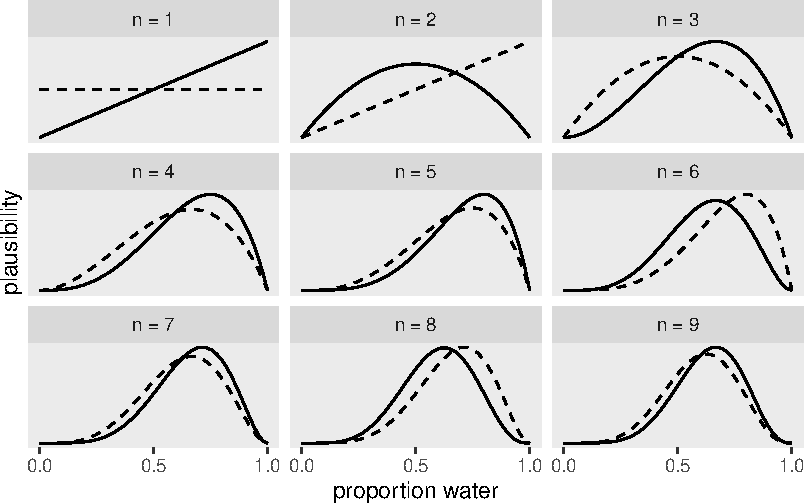
\includegraphics{02-small-and-large-worlds_files/figure-pdf/fig-bayesian-model-learning-anno7-1.pdf}

}

\caption{\label{fig-bayesian-model-learning-anno7}Demonstrating Bayesian
Updating}

\end{figure}

\hypertarget{components-of-the-model}{%
\section{Components of the Model}\label{components-of-the-model}}

\hypertarget{original-3}{%
\subsection{Original}\label{original-3}}

We observed three components of the model:

\begin{enumerate}
\def\labelenumi{\arabic{enumi}.}
\item
  a \textbf{likelihood function}: ``the number of ways each conjecture
  could produce an observation,''
\item
  one or more \textbf{parameters}: ``the accumulated number of ways each
  conjecture could produce the entire data,'' and
\item
  \textbf{a prior}: ``the initial plausibility of each conjectured cause
  of the data''
\end{enumerate}

\hypertarget{list-variables}{%
\subsubsection{List Variables}\label{list-variables}}

\begin{quote}
Variables are just symbols that can take on different values. In a
scientific context, variables include things we wish to infer, such as
proportions and rates, as well as things we might observe, the
data\ldots.

Unobserved variables are usually called \textbf{parameters}. (emphasis
in the original)
\end{quote}

Take as example the globe tossing models: There are three variables:
\texttt{W} and \texttt{L} (water or land) and the proportion of water
and land \texttt{p}. We observe the events of water or land but we
calculate (do not observe directly) the proportion of water and land. So
\texttt{p} is a parameter as defined above.

\hypertarget{define-variables}{%
\subsubsection{Define Variables}\label{define-variables}}

\begin{quote}
In defining each {[}variable{]}, we build a model that relates the
variables to one another. Remember, the goal is to count all the ways
the data could arise, given the assumptions.
\end{quote}

\hypertarget{observed-variables}{%
\paragraph{Observed Variables}\label{observed-variables}}

For each unobserved variable (parameter) we need to define the relative
number of ways---the probability---that the values of each observed
variable could arise. And then for each unobserved variable, we need to
define the prior plausibility of each value it could take.

For the count of water \emph{W} and land \emph{L} in the globe tossing
model, we \textbf{define how plausible any combination of \emph{W} and
\emph{L} would be, for a specific value of \emph{p}.} (emphasis is mine)

\textbf{CHANGE OR MOVE THIS PARAGRAPH}: This idea is implemented in the
functions of \texttt{expand()}, \texttt{expand\_grid()} and
\texttt{crossing()} of the \{\textbf{tidyr}\} package: They generate all
combinations of variables found as is demonstrated in the section
\protect\hyperlink{sec-expand_grid}{Bayesian Updating of the
brms-variant}.

Instead of counting we can also use a mathematical function to calculate
the probability of all combinations. A distribution function assigned to
an observed variable is usually called a \textbf{LIKELIHOOD}.

In the case of the globe-tossing model the appropriate distributional
function is the \textbf{binomial distribution}. (Does this means that I
have to know more on probability theory to decide when to choose which
distribution?)

\textbf{Likelihood for prob = 0.5}

The likelihood in the globe-tossing example (9 trials, 6 with \texttt{W}
and 3 with \texttt{L}) is easily computed:

\begin{Shaded}
\begin{Highlighting}[]
\InformationTok{\textasciigrave{}\textasciigrave{}\textasciigrave{}\{r\}}
\CommentTok{\#| label: likelihood{-}prob{-}0.5{-}a}

\DocumentationTok{\#\# R code 2.2}
\FunctionTok{dbinom}\NormalTok{(}\DecValTok{6}\NormalTok{, }\AttributeTok{size =} \DecValTok{9}\NormalTok{, }\AttributeTok{prob =} \FloatTok{0.5}\NormalTok{)}
\InformationTok{\textasciigrave{}\textasciigrave{}\textasciigrave{}}
\end{Highlighting}
\end{Shaded}

\begin{verbatim}
#> [1] 0.1640625
\end{verbatim}

In this example it is assumed that the probability of \texttt{W} and
\texttt{L} are equal distributed. We calculated how plausible the
combination of \emph{6W} and \emph{3L} would be, for the specific value
of \emph{p = 0.5}. The result is with 16\% a pretty low probability.

\textbf{Likelihood for many prob values}

To get a better idea what the best estimation of the probability is, we
could vary systematically the \texttt{p} value and look for the maximum.
A demonstration how this is done can be seen in
Section~\ref{sec-calcu-10-probs}. It shows a maximum at \emph{prob =
0.7}.

\hypertarget{unobserved-variables}{%
\paragraph{Unobserved Variables}\label{unobserved-variables}}

Even variables that are not observed (= parameters) we need to define
them. In the globe-tossing model there is only one parameter (p), but
most models have more than one unobserved variables.

\begin{quote}
In future chapters, there will be more parameters in your models. In
statistical modeling, many of the most common questions we ask about
data are answered directly by parameters:

\begin{itemize}
\tightlist
\item
  What is the average difference between treatment groups?
\item
  How strong is the association between a treatment and an outcome?
\item
  Does the effect of the treatment depend upon a covariate?
\item
  How much variation is there among groups?
\end{itemize}

{[}We will{]} see how these questions become extra parameters inside the
distribution function we assign to the data.
\end{quote}

\begin{tcolorbox}[enhanced jigsaw, colframe=quarto-callout-important-color-frame, colback=white, toprule=.15mm, breakable, arc=.35mm, bottomtitle=1mm, colbacktitle=quarto-callout-important-color!10!white, toptitle=1mm, titlerule=0mm, title=\textcolor{quarto-callout-important-color}{\faExclamation}\hspace{0.5em}{Parameter \& Prior}, leftrule=.75mm, opacityback=0, rightrule=.15mm, opacitybacktitle=0.6, bottomrule=.15mm, left=2mm, coltitle=black]

For every parameter we must provide a distribution of prior
plausibility, its Prior. This is also true when the number of trials is
null (N = 0), e.g.~even in the initial state of information we need a
prior.

\end{tcolorbox}

When you have a previous estimate, that can become the prior. As a
result, each estimate (posterior probability) becomes then the prior for
the next step. Where do priors come from? They are both engineering
assumptions, chosen to help the machine learn, and scientific
assumptions, chosen to reflect what we know about a phenomenon. Because
the prior is an assumption, it should be interrogated like other
assumptions: by altering it and checking how sensitive inference is to
the assumption.

\begin{tcolorbox}[enhanced jigsaw, colframe=quarto-callout-note-color-frame, colback=white, toprule=.15mm, breakable, arc=.35mm, bottomtitle=1mm, colbacktitle=quarto-callout-note-color!10!white, toptitle=1mm, titlerule=0mm, title=\textcolor{quarto-callout-note-color}{\faInfo}\hspace{0.5em}{Data or Parameters}, leftrule=.75mm, opacityback=0, rightrule=.15mm, opacitybacktitle=0.6, bottomrule=.15mm, left=2mm, coltitle=black]

Data are measured and known; parameters are unknown and must be
estimated from data. But there is a deep identity between certainty
(data) and uncertainty (parameters): Sometimes we observe a variable
(data), sometimes not (parameter) but it could be that the same
distribution function applies. An exploitation of the identity between
data \& parameters is it to incorporate measurement error and missing
data into your modeling.

\begin{tcolorbox}[enhanced jigsaw, colframe=quarto-callout-tip-color-frame, colback=white, toprule=.15mm, breakable, arc=.35mm, bottomtitle=1mm, colbacktitle=quarto-callout-tip-color!10!white, toptitle=1mm, titlerule=0mm, title=\textcolor{quarto-callout-tip-color}{\faLightbulb}\hspace{0.5em}{Tip}, leftrule=.75mm, opacityback=0, rightrule=.15mm, opacitybacktitle=0.6, bottomrule=.15mm, left=2mm, coltitle=black]

For more in this topic, check out McElreath's lecture,
\href{https://youtu.be/yakg94HyWdE}{\emph{Understanding Bayesian
statistics without frequentist language}}.

\end{tcolorbox}

\end{tcolorbox}

\hypertarget{a-model-is-born}{%
\subsubsection{A Model is Born}\label{a-model-is-born}}

\begin{quote}
The observed variables \emph{W} and \emph{L} are given relative counts
through the binomial distribution.
\end{quote}

\[W∼Binomial(n,p)\space where\space N = W + L\]

The above is just a convention for communicating the assumption that the
relative counts of ways to realize \emph{W} in \emph{N} trials with
probability \emph{p} on each trial comes from the binomial distribution.

Our binomial likelihood contains a parameter for an unobserved variable,
\emph{p}. Parameters in Bayesian models are assigned priors:

\[p∼Uniform(0,1)\]

which expresses the model assumption that the entire range of possible
values for p are equally plausible.

\hypertarget{tidyverse-3}{%
\subsection{Tidyverse}\label{tidyverse-3}}

Given a probability of .5, (e.g.~equal probability to both events
\texttt{W} and \texttt{L}) we can use the \texttt{dbinom()} function to
determine the likelihood of 6 out of 9 tosses coming out water.

\begin{Shaded}
\begin{Highlighting}[]
\InformationTok{\textasciigrave{}\textasciigrave{}\textasciigrave{}\{r\}}
\CommentTok{\#| label: likelihood{-}prob{-}0.5{-}b}

\FunctionTok{dbinom}\NormalTok{(}\AttributeTok{x =} \DecValTok{6}\NormalTok{, }\AttributeTok{size =} \DecValTok{9}\NormalTok{, }\AttributeTok{prob =} \FloatTok{0.5}\NormalTok{)}
\InformationTok{\textasciigrave{}\textasciigrave{}\textasciigrave{}}
\end{Highlighting}
\end{Shaded}

\begin{verbatim}
#> [1] 0.1640625
\end{verbatim}

McElreath suggests:

\begin{quote}
Change the 0.5 to any other value, to see how the value changes.
\end{quote}

\hypertarget{sec-calcu-10-probs}{%
\subsubsection{Calculation likelihood with 10 different values of
prob}\label{sec-calcu-10-probs}}

\begin{Shaded}
\begin{Highlighting}[]
\InformationTok{\textasciigrave{}\textasciigrave{}\textasciigrave{}\{r\}}
\CommentTok{\#| label: likelihood{-}10{-}probs}

\NormalTok{(d }\OtherTok{\textless{}{-}} \FunctionTok{tibble}\NormalTok{(}\AttributeTok{prob =} \FunctionTok{seq}\NormalTok{(}\AttributeTok{from =} \DecValTok{0}\NormalTok{, }\AttributeTok{to =} \DecValTok{1}\NormalTok{, }\AttributeTok{by =}\NormalTok{ .}\DecValTok{1}\NormalTok{)) }\SpecialCharTok{|\textgreater{}} 
    \FunctionTok{mutate}\NormalTok{(}\AttributeTok{likelihood =} \FunctionTok{dbinom}\NormalTok{(}\AttributeTok{x =} \DecValTok{6}\NormalTok{, }\AttributeTok{size =} \DecValTok{9}\NormalTok{, }\AttributeTok{prob =}\NormalTok{ prob))}
\NormalTok{)}
\InformationTok{\textasciigrave{}\textasciigrave{}\textasciigrave{}}
\end{Highlighting}
\end{Shaded}

\begin{verbatim}
#> # A tibble: 11 x 2
#>     prob likelihood
#>    <dbl>      <dbl>
#>  1   0    0        
#>  2   0.1  0.0000612
#>  3   0.2  0.00275  
#>  4   0.3  0.0210   
#>  5   0.4  0.0743   
#>  6   0.5  0.164    
#>  7   0.6  0.251    
#>  8   0.7  0.267    
#>  9   0.8  0.176    
#> 10   0.9  0.0446   
#> 11   1    0
\end{verbatim}

Filter the row with the \texttt{prob} maximum.

\begin{Shaded}
\begin{Highlighting}[]
\InformationTok{\textasciigrave{}\textasciigrave{}\textasciigrave{}\{r\}}
\CommentTok{\#| label: filter{-}max}

\NormalTok{d  }\SpecialCharTok{|\textgreater{}}  
    \FunctionTok{filter}\NormalTok{(likelihood }\SpecialCharTok{==} \FunctionTok{max}\NormalTok{(likelihood))}
\InformationTok{\textasciigrave{}\textasciigrave{}\textasciigrave{}}
\end{Highlighting}
\end{Shaded}

\begin{verbatim}
#> # A tibble: 1 x 2
#>    prob likelihood
#>   <dbl>      <dbl>
#> 1   0.7      0.267
\end{verbatim}

In the series of values you will notice several point:

\begin{enumerate}
\def\labelenumi{\arabic{enumi}.}
\tightlist
\item
  The values start with zero until a maximum of 0.267 and decline to
  zero again. The maximum is with \texttt{prob\ =\ 0.7}, a proportion of
  \texttt{W} and \texttt{L} that is --- as we know from our large world
  knowledge (knowledge outside the small world of the model) --- already
  pretty near the real distribution of about 0.71. (see
  \href{https://www.thedailyeco.com/how-much-of-the-earth-is-covered-by-water-122.html}{How
  Much of the Earth Is Covered by Water?})
\item
  You see that the first prob (0) and last prob (1) values are both
  zero. From the result (6 \texttt{W} and 3 \texttt{L}) prob cannot be 0
  or 1 because there a both \texttt{W} and \texttt{L} in the observed
  sample.
\end{enumerate}

The above code chunk is my interpretation from the quote ``Change the
0.5 to any other value, to see how the value changes.'' Kurz has another
interpretation when he draws a graph of 100 prob values from 0 to 1:

\hypertarget{sec-likelihood-for-many-p-values-b}{%
\subsubsection{Plot likelihood for 100 values of
prob}\label{sec-likelihood-for-many-p-values-b}}

\begin{Shaded}
\begin{Highlighting}[]
\InformationTok{\textasciigrave{}\textasciigrave{}\textasciigrave{}\{r\}}
\CommentTok{\#| label: fig{-}likelihood{-}100{-}prob}
\CommentTok{\#| fig{-}cap: "Likelihood for 100 values of prob, from 0 to 1, by steps of 0.01"}

\FunctionTok{tibble}\NormalTok{(}\AttributeTok{prob =} \FunctionTok{seq}\NormalTok{(}\AttributeTok{from =} \DecValTok{0}\NormalTok{, }\AttributeTok{to =} \DecValTok{1}\NormalTok{, }\AttributeTok{by =}\NormalTok{ .}\DecValTok{01}\NormalTok{)) }\SpecialCharTok{\%\textgreater{}\%} 
  \FunctionTok{ggplot}\NormalTok{(}\FunctionTok{aes}\NormalTok{(}\AttributeTok{x =}\NormalTok{ prob, }\AttributeTok{y =} \FunctionTok{dbinom}\NormalTok{(}\AttributeTok{x =} \DecValTok{6}\NormalTok{, }\AttributeTok{size =} \DecValTok{9}\NormalTok{, }\AttributeTok{prob =}\NormalTok{ prob))) }\SpecialCharTok{+}
  \FunctionTok{geom\_line}\NormalTok{() }\SpecialCharTok{+}
  \FunctionTok{labs}\NormalTok{(}\AttributeTok{x =} \StringTok{"probability"}\NormalTok{,}
       \AttributeTok{y =} \StringTok{"binomial likelihood"}\NormalTok{) }\SpecialCharTok{+}
  \FunctionTok{theme}\NormalTok{(}\AttributeTok{panel.grid =} \FunctionTok{element\_blank}\NormalTok{())}
\InformationTok{\textasciigrave{}\textasciigrave{}\textasciigrave{}}
\end{Highlighting}
\end{Shaded}

\begin{figure}[H]

{\centering 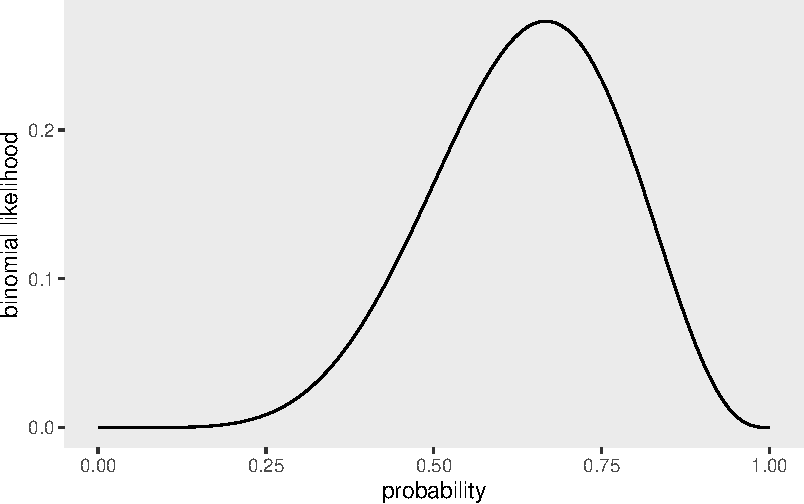
\includegraphics{02-small-and-large-worlds_files/figure-pdf/fig-likelihood-100-prob-1.pdf}

}

\caption{\label{fig-likelihood-100-prob}Likelihood for 100 values of
prob, from 0 to 1, by steps of 0.01}

\end{figure}

In contrast to \emph{p = 0.5} with a probability of 0.16 the
Picture~\ref{fig-likelihood-100-prob} shows a maximum at about \emph{p =
0.7} and a probability estimated from the graph of about 0.26-0.28. We
will get more detailed data later in the book.

It is interesting to see that even the maximum probability is not very
high. The reason is that there are many other configurations
(distributions of \texttt{W}s and \texttt{L}s) to produce the result of
\emph{6W} and \emph{3L}. Even if all these other distributions have a
small probability they ``eat'' all with their share from the maximum.

(I wanted to write ``from the maximum of 1.0'' but I think this would
not be correct as the above graph displays the rate of change in
cumulative probability (the \textbf{probability density}) and not the
probability itself (the \textbf{probability mass}). See the following
quote:

\begin{quote}
For mathematical reasons, probability densities can be greater than 1.
\ldots{} Probability \emph{density} is the rate of change in cumulative
probability. So where cumulative probability is increasing rapidly,
density can easily exceed 1. But if we calculate the area under the
density function, it will never exceed 1. Such areas are also called
\emph{probability mass}. (11.47 in calibre ebook-viewer reference mode)
\end{quote}

In the literature the abbreviation \textbf{PDF
(\href{https://en.wikipedia.org/wiki/Probability_density_function}{probability
density function})} is often used for the (probability) density. See
also th Wikipedia entry about
\href{https://en.wikipedia.org/wiki/Probability_distribution}{probability
distribution}.

McElreath says:

\begin{quote}
The prior is a probability distribution for the parameter. In general,
for a uniform prior from \emph{a} to \emph{b}, the probability of any
point in the interval is 1/(\emph{b -- a}). If you're bothered by the
fact that the probability of every value of \emph{p} is 1, remember that
every probability distribution must sum (integrate) to 1. The expression
1/(\emph{b -- a}) ensures that the area under the flat line from
\emph{a} to \emph{b} is equal to 1.
\end{quote}

Kurz demonstrated the truth of this quote with several \emph{b} values
while holding \emph{a} constant:

\begin{Shaded}
\begin{Highlighting}[]
\InformationTok{\textasciigrave{}\textasciigrave{}\textasciigrave{}\{r\}}
\CommentTok{\#| label: uniform{-}prior1}

\FunctionTok{tibble}\NormalTok{(}\AttributeTok{a =} \DecValTok{0}\NormalTok{,}
       \AttributeTok{b =} \FunctionTok{c}\NormalTok{(}\DecValTok{1}\NormalTok{, }\FloatTok{1.5}\NormalTok{, }\DecValTok{2}\NormalTok{, }\DecValTok{3}\NormalTok{, }\DecValTok{9}\NormalTok{)) }\SpecialCharTok{\%\textgreater{}\%} 
  \FunctionTok{mutate}\NormalTok{(}\AttributeTok{prob =} \DecValTok{1} \SpecialCharTok{/}\NormalTok{ (b }\SpecialCharTok{{-}}\NormalTok{ a))}
\InformationTok{\textasciigrave{}\textasciigrave{}\textasciigrave{}}
\end{Highlighting}
\end{Shaded}

\begin{verbatim}
#> # A tibble: 5 x 3
#>       a     b  prob
#>   <dbl> <dbl> <dbl>
#> 1     0   1   1    
#> 2     0   1.5 0.667
#> 3     0   2   0.5  
#> 4     0   3   0.333
#> 5     0   9   0.111
\end{verbatim}

Verified with a plot he divides the range of the \emph{b} parameter
(\emph{0-9}) into 500 segments (\emph{parameter\_space}) and uses the
\texttt{dunif()} distribution to calculate the probabilities for a
uniform distribution:

\begin{Shaded}
\begin{Highlighting}[]
\InformationTok{\textasciigrave{}\textasciigrave{}\textasciigrave{}\{r\}}
\CommentTok{\#| label: uniform{-}prior2}

\FunctionTok{tibble}\NormalTok{(}\AttributeTok{a =} \DecValTok{0}\NormalTok{,}
       \AttributeTok{b =} \FunctionTok{c}\NormalTok{(}\DecValTok{1}\NormalTok{, }\FloatTok{1.5}\NormalTok{, }\DecValTok{2}\NormalTok{, }\DecValTok{3}\NormalTok{, }\DecValTok{9}\NormalTok{)) }\SpecialCharTok{\%\textgreater{}\%} 
  \FunctionTok{expand\_grid}\NormalTok{(}\AttributeTok{parameter\_space =} \FunctionTok{seq}\NormalTok{(}\AttributeTok{from =} \DecValTok{0}\NormalTok{, }\AttributeTok{to =} \DecValTok{9}\NormalTok{, }\AttributeTok{length.out =} \DecValTok{500}\NormalTok{)) }\SpecialCharTok{\%\textgreater{}\%} 
  \FunctionTok{mutate}\NormalTok{(}\AttributeTok{prob =} \FunctionTok{dunif}\NormalTok{(parameter\_space, a, b),}
         \AttributeTok{b    =} \FunctionTok{str\_c}\NormalTok{(}\StringTok{"b = "}\NormalTok{, b)) }\SpecialCharTok{\%\textgreater{}\%} 
  
  \FunctionTok{ggplot}\NormalTok{(}\FunctionTok{aes}\NormalTok{(}\AttributeTok{x =}\NormalTok{ parameter\_space, }\AttributeTok{y =}\NormalTok{ prob)) }\SpecialCharTok{+}
  \FunctionTok{geom\_area}\NormalTok{() }\SpecialCharTok{+}
  \FunctionTok{scale\_x\_continuous}\NormalTok{(}\AttributeTok{breaks =} \FunctionTok{c}\NormalTok{(}\DecValTok{0}\NormalTok{, }\DecValTok{1}\SpecialCharTok{:}\DecValTok{3}\NormalTok{, }\DecValTok{9}\NormalTok{)) }\SpecialCharTok{+}
  \FunctionTok{scale\_y\_continuous}\NormalTok{(}\AttributeTok{breaks =} \FunctionTok{c}\NormalTok{(}\DecValTok{0}\NormalTok{, }\DecValTok{1}\SpecialCharTok{/}\DecValTok{9}\NormalTok{, }\DecValTok{1}\SpecialCharTok{/}\DecValTok{3}\NormalTok{, }\DecValTok{1}\SpecialCharTok{/}\DecValTok{2}\NormalTok{, }\DecValTok{2}\SpecialCharTok{/}\DecValTok{3}\NormalTok{, }\DecValTok{1}\NormalTok{),}
                     \AttributeTok{labels =} \FunctionTok{c}\NormalTok{(}\StringTok{"0"}\NormalTok{, }\StringTok{"1/9"}\NormalTok{, }\StringTok{"1/3"}\NormalTok{, }\StringTok{"1/2"}\NormalTok{, }\StringTok{"2/3"}\NormalTok{, }\StringTok{"1"}\NormalTok{)) }\SpecialCharTok{+}
  \FunctionTok{theme}\NormalTok{(}\AttributeTok{panel.grid.minor =} \FunctionTok{element\_blank}\NormalTok{(),}
        \AttributeTok{panel.grid.major.x =} \FunctionTok{element\_blank}\NormalTok{()) }\SpecialCharTok{+}
  \FunctionTok{facet\_wrap}\NormalTok{(}\SpecialCharTok{\textasciitilde{}}\NormalTok{ b, }\AttributeTok{ncol =} \DecValTok{5}\NormalTok{)}
\InformationTok{\textasciigrave{}\textasciigrave{}\textasciigrave{}}
\end{Highlighting}
\end{Shaded}

\begin{figure}[H]

{\centering 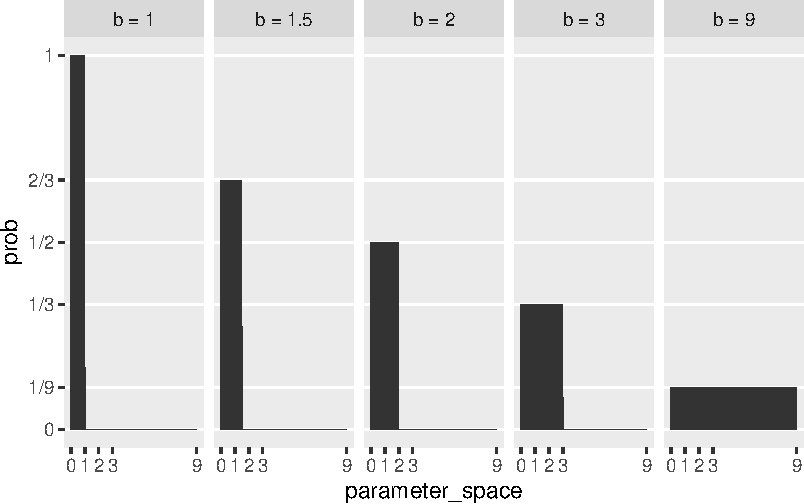
\includegraphics{02-small-and-large-worlds_files/figure-pdf/uniform-prior2-1.pdf}

}

\end{figure}

This figure demonstrates that the area in the whole paramater space is
\emph{1.0}. It is a nice example how to calculate the probability
\emph{mass} (in contrast to the curve of the probability
\emph{density}).

I will skip the excursus and plot about the equivalence of
\texttt{Uniform(0,1)} and the beta distribution calculated with
\texttt{dbeta().}

\hypertarget{making-the-model-go}{%
\section{Making the Model Go}\label{making-the-model-go}}

\hypertarget{bayes-theorem}{%
\subsection{Bayes' Theorem}\label{bayes-theorem}}

\hypertarget{original-4}{%
\subsubsection{Original}\label{original-4}}

\begin{quote}
Once you have named all the variables and chosen definitions for each, a
Bayesian model can update all of the prior distributions to their purely
logical consequences: the \textbf{POSTERIOR DISTRIBUTION}. For every
unique combination of data, likelihood, parameters, and prior, there is
a unique posterior distribution. This distribution contains the relative
plausibility of different parameter values, conditional on the data and
model. The posterior distribution takes the form of the probability of
the parameters, conditional on the data.
\end{quote}

In the case of the globe-tossing model we can write:

\[
Pr(p|W, L)
\]

This has to be interpreted as ``the probability of each possible value
of \emph{p}, conditional on the specific \emph{W} and \emph{L} that we
observed.''

\[
Pr(p|W,L) = \frac{Pr(W,L|p)Pr(p)}{Pr(W,L)}
\]

\begin{quote}
And this is Bayes' theorem. It says that the probability of any
particular value of \emph{p}, considering the data, is equal to the
product of the relative plausibility of the data, conditional on
\emph{p}, and the prior plausibility of \emph{p}, divided by this thing
Pr(\emph{W, L}), which I'll call the \emph{average probability of the
data}.
\end{quote}

Expressed in words:

\[
Posterior = \frac{Probability\space of\space the\space data\space ✕\space Prior}{Average\space probability\space of\space the\space data}
\]

Other names for the \emph{average probability of the data}:

\begin{itemize}
\tightlist
\item
  evidence
\item
  average likelihood
\item
  marginal likelihood
\end{itemize}

The job of the average probability of the data is just to standardize
the posterior, to ensure it sums (integrates) to one.

\begin{tcolorbox}[enhanced jigsaw, colframe=quarto-callout-important-color-frame, colback=white, toprule=.15mm, breakable, arc=.35mm, bottomtitle=1mm, colbacktitle=quarto-callout-important-color!10!white, toptitle=1mm, titlerule=0mm, title=\textcolor{quarto-callout-important-color}{\faExclamation}\hspace{0.5em}{Key lesson}, leftrule=.75mm, opacityback=0, rightrule=.15mm, opacitybacktitle=0.6, bottomrule=.15mm, left=2mm, coltitle=black]

The posterior is proportional to the product of the prior and the
probability of the data.

\end{tcolorbox}

\begin{quote}
{[}E{]}ach specific value of \emph{p}, the number of paths through the
garden of forking data is the product of the prior number of paths and
the new number of paths. \textbf{Multiplication is just compressed
counting.} The average probability on the bottom just standardizes the
counts so they sum to one. (emphasis is mine)
\end{quote}

\begin{quote}
{[}The following graph{]} illustrates the multiplicative interaction of
a prior and a probability of data. On each row, a prior on the left is
multiplied by the probability of data in the middle to produce a
posterior on the right. The probability of data in each case is the
same. The priors however vary. As a result, the posterior distributions
vary.
\end{quote}

\begin{figure}

{\centering 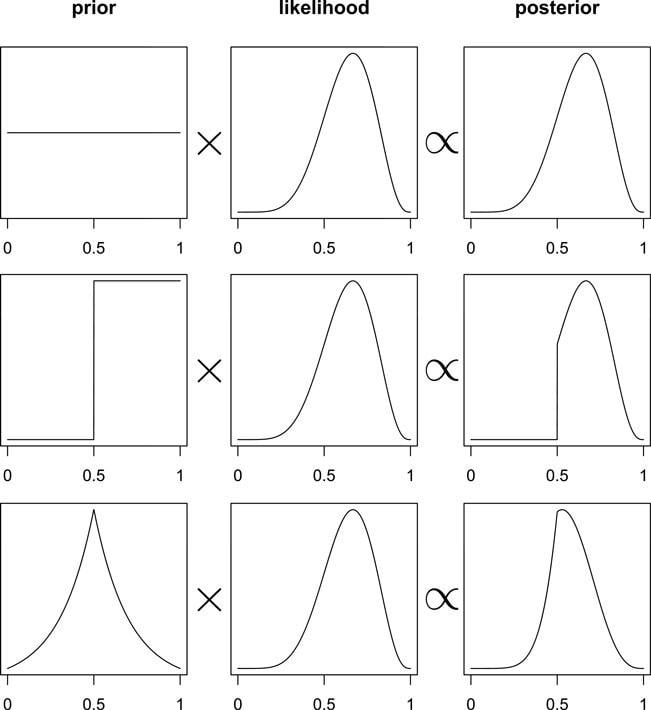
\includegraphics{img/SR2-fig2_6-min.jpg}

}

\caption{\label{fig-2-6-book}Figure 2.6 of the original book}

\end{figure}

For my understanding it is important to reproduce the above graph with R
code as it is shown in the next section.

\hypertarget{tidyverse-4}{%
\subsubsection{Tidyverse}\label{tidyverse-4}}

\begin{quote}
{[}The following graph{]} illustrates the multiplicative interaction of
a prior and a probability of data. On each row, a prior on the left is
multiplied by the probability of data in the middle to produce a
posterior on the right. The probability of data in each case is the
same. The priors however vary. As a result, the posterior distributions
vary.
\end{quote}

\begin{codelisting}

\caption{The posterior distribution as a product of the prior
distribution and likelihood.}

\hypertarget{lst-prepare-model}{%
\label{lst-prepare-model}}%
\begin{Shaded}
\begin{Highlighting}[]
\InformationTok{\textasciigrave{}\textasciigrave{}\textasciigrave{}\{r\}}
\CommentTok{\#| label: prepare{-}model}
\CommentTok{\#| attr{-}source: \textquotesingle{}\#lst{-}prepare{-}model lst{-}cap="The posterior distribution as a product of the prior distribution and likelihood."\textquotesingle{}}

\NormalTok{sequence\_length }\OtherTok{\textless{}{-}} \FloatTok{1e3}

\NormalTok{d }\OtherTok{\textless{}{-}}
  \FunctionTok{tibble}\NormalTok{(}\AttributeTok{probability =} \FunctionTok{seq}\NormalTok{(}\AttributeTok{from =} \DecValTok{0}\NormalTok{, }\AttributeTok{to =} \DecValTok{1}\NormalTok{, }\AttributeTok{length.out =}\NormalTok{ sequence\_length)) }\SpecialCharTok{\%\textgreater{}\%} 
  \FunctionTok{expand\_grid}\NormalTok{(}\AttributeTok{row =} \FunctionTok{c}\NormalTok{(}\StringTok{"flat"}\NormalTok{, }\StringTok{"stepped"}\NormalTok{, }\StringTok{"Laplace"}\NormalTok{))  }\SpecialCharTok{\%\textgreater{}\%} 
  \FunctionTok{arrange}\NormalTok{(row, probability) }\SpecialCharTok{\%\textgreater{}\%} 
  \FunctionTok{mutate}\NormalTok{(}\AttributeTok{prior =} \FunctionTok{ifelse}\NormalTok{(row }\SpecialCharTok{==} \StringTok{"flat"}\NormalTok{, }\DecValTok{1}\NormalTok{,}
                        \FunctionTok{ifelse}\NormalTok{(row }\SpecialCharTok{==} \StringTok{"stepped"}\NormalTok{, }\FunctionTok{rep}\NormalTok{(}\DecValTok{0}\SpecialCharTok{:}\DecValTok{1}\NormalTok{, }\AttributeTok{each =}\NormalTok{ sequence\_length }\SpecialCharTok{/} \DecValTok{2}\NormalTok{),}
                               \FunctionTok{exp}\NormalTok{(}\SpecialCharTok{{-}}\FunctionTok{abs}\NormalTok{(probability }\SpecialCharTok{{-}} \FloatTok{0.5}\NormalTok{) }\SpecialCharTok{/}\NormalTok{ .}\DecValTok{25}\NormalTok{) }\SpecialCharTok{/}\NormalTok{ ( }\DecValTok{2} \SpecialCharTok{*} \FloatTok{0.25}\NormalTok{))),}
         \AttributeTok{likelihood =} \FunctionTok{dbinom}\NormalTok{(}\AttributeTok{x =} \DecValTok{6}\NormalTok{, }\AttributeTok{size =} \DecValTok{9}\NormalTok{, }\AttributeTok{prob =}\NormalTok{ probability)) }\SpecialCharTok{\%\textgreater{}\%} 
  \FunctionTok{group\_by}\NormalTok{(row) }\SpecialCharTok{\%\textgreater{}\%} 
  \FunctionTok{mutate}\NormalTok{(}\AttributeTok{posterior =}\NormalTok{ prior }\SpecialCharTok{*}\NormalTok{ likelihood }\SpecialCharTok{/} \FunctionTok{sum}\NormalTok{(prior }\SpecialCharTok{*}\NormalTok{ likelihood)) }\SpecialCharTok{\%\textgreater{}\%} 
  \FunctionTok{pivot\_longer}\NormalTok{(prior}\SpecialCharTok{:}\NormalTok{posterior)  }\SpecialCharTok{\%\textgreater{}\%} 
  \FunctionTok{ungroup}\NormalTok{() }\SpecialCharTok{\%\textgreater{}\%} 
  \FunctionTok{mutate}\NormalTok{(}\AttributeTok{name =} \FunctionTok{factor}\NormalTok{(name, }\AttributeTok{levels =} \FunctionTok{c}\NormalTok{(}\StringTok{"prior"}\NormalTok{, }\StringTok{"likelihood"}\NormalTok{, }\StringTok{"posterior"}\NormalTok{)),}
         \AttributeTok{row  =} \FunctionTok{factor}\NormalTok{(row, }\AttributeTok{levels =} \FunctionTok{c}\NormalTok{(}\StringTok{"flat"}\NormalTok{, }\StringTok{"stepped"}\NormalTok{, }\StringTok{"Laplace"}\NormalTok{)))}
\InformationTok{\textasciigrave{}\textasciigrave{}\textasciigrave{}}
\end{Highlighting}
\end{Shaded}

\end{codelisting}

In comparison to my very detailed code annotations of
Picture~\ref{fig-bayesian-model-learning} there are different lines of
code, but generally there is nothing conceptually new: We use again
\texttt{expand\_grid()} to create a tibble of input combinations and
create with \texttt{mutate()} two columns for prior and likelihood. We
do not use the \texttt{lag()} functions as we calculate only for one
prior and one likelihood. Kurz advises us that is ``easier to just make
each column of the plot separately. We can then use the elegant and
powerful syntax from \href{https://www.data-imaginist.com/}{Thomas Lin
Pedersen}'s (2022)
\href{https://patchwork.data-imaginist.com/}{patchwork package} to
combine them.''

\begin{Shaded}
\begin{Highlighting}[]
\InformationTok{\textasciigrave{}\textasciigrave{}\textasciigrave{}\{r\}}
\CommentTok{\#| label: fig{-}plot{-}model}
\CommentTok{\#| fig{-}cap: "Figure 2.6 from book reproduced with tidyverse code shows the posterior distribution as a product of the prior distribution and likelihood. Top: A flat prior constructs a posterior that is simply proportional to the likelihood. Middle: A step prior, assigning zero probability to all values less than 0.5, results in a truncated posterior. Bottom: A peaked prior that shifts and skews the posterior, relative to the likelihood. Cormpare it with @fig{-}2{-}6{-}book."}

\NormalTok{p1 }\OtherTok{\textless{}{-}}
\NormalTok{  d }\SpecialCharTok{\%\textgreater{}\%}
  \FunctionTok{filter}\NormalTok{(row }\SpecialCharTok{==} \StringTok{"flat"}\NormalTok{) }\SpecialCharTok{\%\textgreater{}\%} 
  \FunctionTok{ggplot}\NormalTok{(}\FunctionTok{aes}\NormalTok{(}\AttributeTok{x =}\NormalTok{ probability, }\AttributeTok{y =}\NormalTok{ value)) }\SpecialCharTok{+}
  \FunctionTok{geom\_line}\NormalTok{() }\SpecialCharTok{+}
  \FunctionTok{scale\_x\_continuous}\NormalTok{(}\ConstantTok{NULL}\NormalTok{, }\AttributeTok{breaks =} \ConstantTok{NULL}\NormalTok{) }\SpecialCharTok{+}
  \FunctionTok{scale\_y\_continuous}\NormalTok{(}\ConstantTok{NULL}\NormalTok{, }\AttributeTok{breaks =} \ConstantTok{NULL}\NormalTok{) }\SpecialCharTok{+}
  \FunctionTok{theme}\NormalTok{(}\AttributeTok{panel.grid =} \FunctionTok{element\_blank}\NormalTok{()) }\SpecialCharTok{+}
  \FunctionTok{facet\_wrap}\NormalTok{(}\SpecialCharTok{\textasciitilde{}}\NormalTok{ name, }\AttributeTok{scales =} \StringTok{"free\_y"}\NormalTok{)}

\NormalTok{p2 }\OtherTok{\textless{}{-}}
\NormalTok{  d }\SpecialCharTok{\%\textgreater{}\%}
  \FunctionTok{filter}\NormalTok{(row }\SpecialCharTok{==} \StringTok{"stepped"}\NormalTok{) }\SpecialCharTok{\%\textgreater{}\%} 
  \FunctionTok{ggplot}\NormalTok{(}\FunctionTok{aes}\NormalTok{(}\AttributeTok{x =}\NormalTok{ probability, }\AttributeTok{y =}\NormalTok{ value)) }\SpecialCharTok{+}
  \FunctionTok{geom\_line}\NormalTok{() }\SpecialCharTok{+}
  \FunctionTok{scale\_x\_continuous}\NormalTok{(}\ConstantTok{NULL}\NormalTok{, }\AttributeTok{breaks =} \ConstantTok{NULL}\NormalTok{) }\SpecialCharTok{+}
  \FunctionTok{scale\_y\_continuous}\NormalTok{(}\ConstantTok{NULL}\NormalTok{, }\AttributeTok{breaks =} \ConstantTok{NULL}\NormalTok{) }\SpecialCharTok{+}
  \FunctionTok{theme}\NormalTok{(}\AttributeTok{panel.grid =} \FunctionTok{element\_blank}\NormalTok{(),}
        \AttributeTok{strip.background =} \FunctionTok{element\_blank}\NormalTok{(),}
        \AttributeTok{strip.text =} \FunctionTok{element\_blank}\NormalTok{()) }\SpecialCharTok{+}
  \FunctionTok{facet\_wrap}\NormalTok{(}\SpecialCharTok{\textasciitilde{}}\NormalTok{ name, }\AttributeTok{scales =} \StringTok{"free\_y"}\NormalTok{)}

\NormalTok{p3 }\OtherTok{\textless{}{-}}
\NormalTok{  d }\SpecialCharTok{\%\textgreater{}\%}
  \FunctionTok{filter}\NormalTok{(row }\SpecialCharTok{==} \StringTok{"Laplace"}\NormalTok{) }\SpecialCharTok{\%\textgreater{}\%} 
  \FunctionTok{ggplot}\NormalTok{(}\FunctionTok{aes}\NormalTok{(}\AttributeTok{x =}\NormalTok{ probability, }\AttributeTok{y =}\NormalTok{ value)) }\SpecialCharTok{+}
  \FunctionTok{geom\_line}\NormalTok{() }\SpecialCharTok{+}
  \FunctionTok{scale\_x\_continuous}\NormalTok{(}\ConstantTok{NULL}\NormalTok{, }\AttributeTok{breaks =} \FunctionTok{c}\NormalTok{(}\DecValTok{0}\NormalTok{, .}\DecValTok{5}\NormalTok{, }\DecValTok{1}\NormalTok{)) }\SpecialCharTok{+}
  \FunctionTok{scale\_y\_continuous}\NormalTok{(}\ConstantTok{NULL}\NormalTok{, }\AttributeTok{breaks =} \ConstantTok{NULL}\NormalTok{) }\SpecialCharTok{+}
  \FunctionTok{theme}\NormalTok{(}\AttributeTok{panel.grid =} \FunctionTok{element\_blank}\NormalTok{(),}
        \AttributeTok{strip.background =} \FunctionTok{element\_blank}\NormalTok{(),}
        \AttributeTok{strip.text =} \FunctionTok{element\_blank}\NormalTok{()) }\SpecialCharTok{+}
  \FunctionTok{facet\_wrap}\NormalTok{(}\SpecialCharTok{\textasciitilde{}}\NormalTok{ name, }\AttributeTok{scales =} \StringTok{"free\_y"}\NormalTok{)}

\CommentTok{\# combine}
\CommentTok{\# library(patchwork) \# defined in setup chunk}
\NormalTok{p1 }\SpecialCharTok{/}\NormalTok{ p2 }\SpecialCharTok{/}\NormalTok{ p3}
\InformationTok{\textasciigrave{}\textasciigrave{}\textasciigrave{}}
\end{Highlighting}
\end{Shaded}

\begin{figure}[H]

{\centering 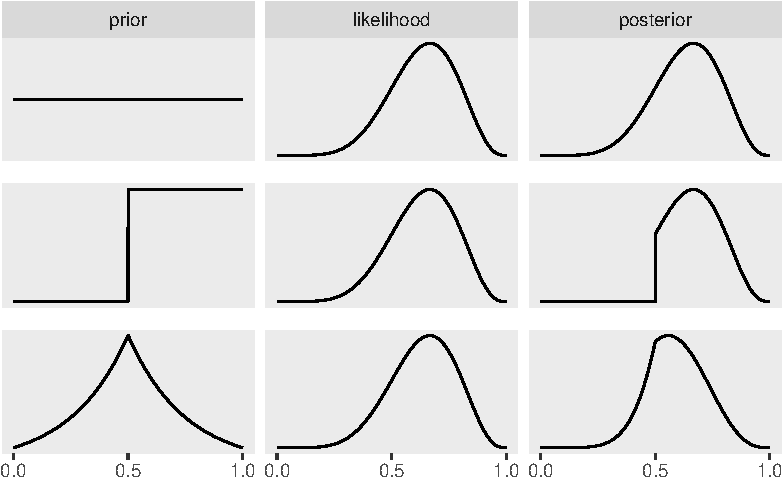
\includegraphics{02-small-and-large-worlds_files/figure-pdf/fig-plot-model-1.pdf}

}

\caption{\label{fig-plot-model}Figure 2.6 from book reproduced with
tidyverse code shows the posterior distribution as a product of the
prior distribution and likelihood. Top: A flat prior constructs a
posterior that is simply proportional to the likelihood. Middle: A step
prior, assigning zero probability to all values less than 0.5, results
in a truncated posterior. Bottom: A peaked prior that shifts and skews
the posterior, relative to the likelihood. Cormpare it with
Picture~\ref{fig-2-6-book}.}

\end{figure}

Picture~\ref{fig-plot-model} shows that the same likelihood with a
different prior results in a different posterior.

\hypertarget{motors}{%
\subsection{Motors}\label{motors}}

\hypertarget{original-5}{%
\subsubsection{Original}\label{original-5}}

\begin{quote}
Recall that your Bayesian model is a machine, a figurative golem. It has
built-in definitions for the likelihood, the parameters, and the prior.
And then at its heart lies a motor that processes data, producing a
posterior distribution. The action of this motor can be thought of as
\emph{conditioning} the prior on the data. As explained in the previous
section, this conditioning is governed by the rules of probability
theory, which defines a uniquely logical posterior for set of
assumptions and observations.

However, knowing the mathematical rule is often of little help, because
many of the interesting models in contemporary science cannot be
conditioned formally, no matter your skill in mathematics. And while
some broadly useful models like linear regression can be conditioned
formally, this is only possible if you constrain your choice of prior to
special forms that are easy to do mathematics with. We'd like to avoid
forced modeling choices of this kind, instead favoring conditioning
engines that can accommodate whichever prior is most useful for
inference.

What this means is that various numerical techniques are needed to
approximate the mathematics that follows from the definition of Bayes'
theorem. In this book, you'll meet three different conditioning engines,
numerical techniques for computing posterior distributions:
\end{quote}

What are the numerical techniques for computing posterior distributions
explained in the book?

\begin{enumerate}
\def\labelenumi{\arabic{enumi}.}
\tightlist
\item
  Grid approximation
\item
  Quadratic approximation
\item
  Markov chain Monte Carlo (MCMC)
\end{enumerate}

\begin{quote}
There are many other engines, and new ones are being invented all the
time. But the three you'll get to know here are common and widely
useful. (p.~39)
\end{quote}

\begin{tcolorbox}[enhanced jigsaw, colframe=quarto-callout-tip-color-frame, colback=white, toprule=.15mm, breakable, arc=.35mm, bottomtitle=1mm, colbacktitle=quarto-callout-tip-color!10!white, toptitle=1mm, titlerule=0mm, title=\textcolor{quarto-callout-tip-color}{\faLightbulb}\hspace{0.5em}{Tip}, leftrule=.75mm, opacityback=0, rightrule=.15mm, opacitybacktitle=0.6, bottomrule=.15mm, left=2mm, coltitle=black]

\textbf{Rethinking: How you fit the model is part of the model}. Earlier
in this chapter, I implicitly defined the model as a composite of a
prior and a likelihood. That definition is typical. But in practical
terms, we should also consider how the model is fit to data as part of
the model. In very simple problems, like the globe tossing example that
consumes this chapter, calculation of the posterior density is trivial
and foolproof. In even moderately complex problems, however, the details
of fitting the model to data force us to recognize that our numerical
technique influences our inferences. This is because different mistakes
and compromises arise under different techniques. The same model fit to
the same data using different techniques may produce different answers.
When something goes wrong, every piece of the machine may be suspect.
And so our golems carry with them their updating engines, as much slaves
to their engineering as they are to the priors and likelihoods we
program into them.

\end{tcolorbox}

\hypertarget{tidyverse-5}{%
\subsubsection{Tidyverse}\label{tidyverse-5}}

In my own words: Processing the built-in definitions for the likelihood,
the parameters, and the prior produces the posterior distribution. This
process is governed by the rule of probability theory. But knowing the
mathematics does generally not help for two reasons:

\begin{itemize}
\tightlist
\item
  Many of the interesting models in contemporary science cannot be
  conditioned formally
\item
  Though some broadly useful models like linear regression can be
  conditioned formally, this is only possible if you constrain your
  choice of prior to special forms that are easy to do mathematics with.
\end{itemize}

Therefore are various numerical techniques needed to approximate the
mathematics that follows from the definition of Bayes' theorem. From the
three widely useful methods (grid approximation, quadratic approximation
and MCMC) covered in the SR2-book the tidyverse version of this material
concentrates on using the
\href{https://paul-buerkner.github.io/brms/}{\{\textbf{brms}\} package}.

\begin{tcolorbox}[enhanced jigsaw, colframe=quarto-callout-caution-color-frame, colback=white, toprule=.15mm, breakable, arc=.35mm, bottomtitle=1mm, colbacktitle=quarto-callout-caution-color!10!white, toptitle=1mm, titlerule=0mm, title=\textcolor{quarto-callout-caution-color}{\faFire}\hspace{0.5em}{Jumping quickly into MCMC}, leftrule=.75mm, opacityback=0, rightrule=.15mm, opacitybacktitle=0.6, bottomrule=.15mm, left=2mm, coltitle=black]

\begin{quote}
The consequence is that this version will jump rather quickly into MCMC.
This will be awkward at times because it will force us to contend with
technical issues in earlier problems in the text than McElreath
originally did.
\end{quote}

\end{tcolorbox}

\hypertarget{grid-approximation}{%
\subsection{Grid approximation}\label{grid-approximation}}

\hypertarget{original-6}{%
\subsubsection{Original}\label{original-6}}

\begin{quote}
While most parameters are \emph{continuous}, capable of taking on an
infinite number of values, it turns out that we can achieve an excellent
approximation of the continuous posterior distribution by considering
only a finite grid of parameter values. At any particular value of a
parameter, \emph{p}', it's a simple matter to compute the posterior
probability: just multiply the prior probability of \emph{p}' by the
likelihood at \emph{p}'. Repeating this procedure for each value in the
grid generates an approximate picture of the exact posterior
distribution. This procedure is called \textbf{GRID APPROXIMATION}.
\end{quote}

Grid approximation is very useful as a pedagogical tool. But in most of
your real modeling, grid approximation isn't practical because it scales
poorly, as the number of parameters increases.

\begin{enumerate}
\def\labelenumi{\arabic{enumi}.}
\tightlist
\item
  Define the grid. This means you decide how many points to use in
  estimating the posterior, and then you make a list of the parameter
  values on the grid.
\item
  Compute the value of the prior at each parameter value on the grid.
\item
  Compute the likelihood at each parameter value.
\item
  Compute the unstandardized posterior at each parameter value, by
  multiplying the prior by the likelihood.
\item
  Finally, standardize the posterior, by dividing each value by the sum
  of all values.
\end{enumerate}

In the globe tossing model the five steps are as follows:

\begin{Shaded}
\begin{Highlighting}[]
\InformationTok{\textasciigrave{}\textasciigrave{}\textasciigrave{}\{r\}}
\CommentTok{\#| label: fig{-}grid{-}approx{-}base1}
\CommentTok{\#| fig{-}cap: "Grid Approximation with 20 points with \textasciigrave{}prior = 1\textasciigrave{}"}

\CommentTok{\# 1. define grid}
\NormalTok{p\_grid }\OtherTok{\textless{}{-}} \FunctionTok{seq}\NormalTok{(}\AttributeTok{from =} \DecValTok{0}\NormalTok{, }\AttributeTok{to =} \DecValTok{1}\NormalTok{, }\AttributeTok{length.out =} \DecValTok{20}\NormalTok{)}

\CommentTok{\# 2. define prior}
\NormalTok{prior }\OtherTok{\textless{}{-}} \FunctionTok{rep}\NormalTok{(}\DecValTok{1}\NormalTok{, }\DecValTok{20}\NormalTok{)}

\CommentTok{\# 3. compute likelihood at each value in grid}
\NormalTok{likelihood }\OtherTok{\textless{}{-}} \FunctionTok{dbinom}\NormalTok{(}\AttributeTok{x =} \DecValTok{6}\NormalTok{, }\AttributeTok{size =} \DecValTok{9}\NormalTok{, }\AttributeTok{prob =}\NormalTok{ p\_grid)}

\CommentTok{\# 4. compute product of likelihood and prior}
\NormalTok{unstd.posterior }\OtherTok{\textless{}{-}}\NormalTok{ likelihood }\SpecialCharTok{*}\NormalTok{ prior}

\CommentTok{\# 5. standardize the posterior, so it sums to 1}
\NormalTok{posterior }\OtherTok{\textless{}{-}}\NormalTok{ unstd.posterior }\SpecialCharTok{/} \FunctionTok{sum}\NormalTok{(unstd.posterior)}

\CommentTok{\# 6 display the posterior distribution}
\DocumentationTok{\#\# R code 2.4}
\FunctionTok{plot}\NormalTok{(p\_grid, posterior,}
  \AttributeTok{type =} \StringTok{"b"}\NormalTok{,}
  \AttributeTok{xlab =} \StringTok{"probability of water"}\NormalTok{, }\AttributeTok{ylab =} \StringTok{"posterior probability"}
\NormalTok{)}
\FunctionTok{mtext}\NormalTok{(}\StringTok{\textquotesingle{}20 points with "prior = 1"\textquotesingle{}}\NormalTok{)}

\InformationTok{\textasciigrave{}\textasciigrave{}\textasciigrave{}}
\end{Highlighting}
\end{Shaded}

\begin{figure}[H]

{\centering 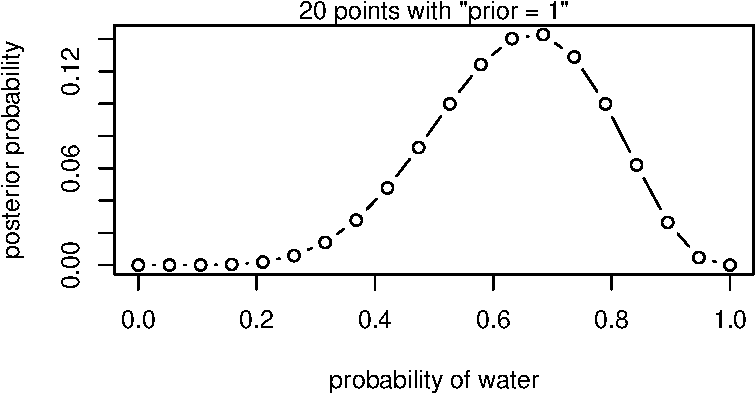
\includegraphics{02-small-and-large-worlds_files/figure-pdf/fig-grid-approx-base1-1.pdf}

}

\caption{\label{fig-grid-approx-base1}Grid Approximation with 20 points
with \texttt{prior\ =\ 1}}

\end{figure}

\begin{Shaded}
\begin{Highlighting}[]
\CommentTok{\#| label: lst{-}own{-}tidyverse}
\CommentTok{\#| lst{-}cap: "My own tidyverse plot \textless{}{-}  just for learning purposes"}

\CommentTok{\# \# instead of books R code 2.4 I will use a tidyverse approach}
\CommentTok{\# df \textless{}{-} dplyr::bind\_cols("prob" = p\_grid, "post" = posterior)}
\CommentTok{\# ggplot2::ggplot(df, ggplot2::aes(x = prob, y = post)) +}
\CommentTok{\#     ggplot2::geom\_line() +}
\CommentTok{\#     ggplot2::geom\_point()}
\end{Highlighting}
\end{Shaded}

\hypertarget{change-likelihood-parameters}{%
\paragraph{Change likelihood
parameters}\label{change-likelihood-parameters}}

The parameters for the calculated likelihood is based on the binomial
distribution and is shaping the above plot:

\begin{itemize}
\tightlist
\item
  x = number of water events \texttt{W}
\item
  size = number of sample trials = number of observations
\item
  prob = success probability on each trial = probability of \texttt{W}
  (water event)
\end{itemize}

It does not matter in the code for Picture~\ref{fig-grid-approx-base1}
what prior probability is chosen in the range from 0 to 1, if the
probability of \texttt{W} is greater than zero and --- and by definition
of the binomial function --- equal for all 20 events. This does not only
conform to values but also for functions.

\begin{Shaded}
\begin{Highlighting}[]
\InformationTok{\textasciigrave{}\textasciigrave{}\textasciigrave{}\{r\}}
\CommentTok{\#| label: fig{-}grid{-}approx{-}base1a}
\CommentTok{\#| fig{-}cap: "Grid Approximation with 20 points with \textasciigrave{}prior = 0.1\textasciigrave{}"}

\CommentTok{\# 1. define grid}
\NormalTok{p\_grid }\OtherTok{\textless{}{-}} \FunctionTok{seq}\NormalTok{(}\AttributeTok{from =} \DecValTok{0}\NormalTok{, }\AttributeTok{to =} \DecValTok{1}\NormalTok{, }\AttributeTok{length.out =} \DecValTok{20}\NormalTok{)}

\CommentTok{\# 2. define prior}
\NormalTok{prior }\OtherTok{\textless{}{-}} \FunctionTok{rep}\NormalTok{(}\FloatTok{0.1}\NormalTok{, }\DecValTok{20}\NormalTok{)}

\CommentTok{\# 3. compute likelihood at each value in grid}
\NormalTok{likelihood }\OtherTok{\textless{}{-}} \FunctionTok{dbinom}\NormalTok{(}\AttributeTok{x =} \DecValTok{6}\NormalTok{, }\AttributeTok{size =} \DecValTok{9}\NormalTok{, }\AttributeTok{prob =}\NormalTok{ p\_grid)}

\CommentTok{\# 4. compute product of likelihood and prior}
\NormalTok{unstd.posterior }\OtherTok{\textless{}{-}}\NormalTok{ likelihood }\SpecialCharTok{*}\NormalTok{ prior}

\CommentTok{\# 5. standardize the posterior, so it sums to 1}
\NormalTok{posterior }\OtherTok{\textless{}{-}}\NormalTok{ unstd.posterior }\SpecialCharTok{/} \FunctionTok{sum}\NormalTok{(unstd.posterior)}

\CommentTok{\# 6 display the posterior distribution}
\DocumentationTok{\#\# R code 2.4}
\FunctionTok{plot}\NormalTok{(p\_grid, posterior,}
  \AttributeTok{type =} \StringTok{"b"}\NormalTok{,}
  \AttributeTok{xlab =} \StringTok{"probability of water"}\NormalTok{, }\AttributeTok{ylab =} \StringTok{"posterior probability"}
\NormalTok{)}
\FunctionTok{mtext}\NormalTok{(}\StringTok{\textquotesingle{}20 points with "prior = 0.1"\textquotesingle{}}\NormalTok{)}
\InformationTok{\textasciigrave{}\textasciigrave{}\textasciigrave{}}
\end{Highlighting}
\end{Shaded}

\begin{figure}[H]

{\centering 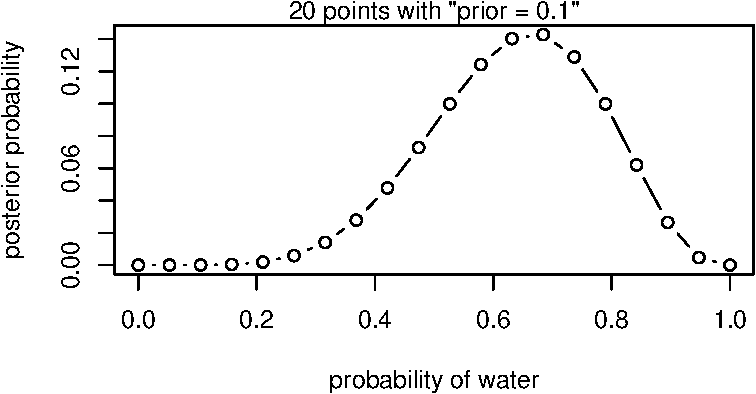
\includegraphics{02-small-and-large-worlds_files/figure-pdf/fig-grid-approx-base1a-1.pdf}

}

\caption{\label{fig-grid-approx-base1a}Grid Approximation with 20 points
with \texttt{prior\ =\ 0.1}}

\end{figure}

\hypertarget{changing-prior-parameters}{%
\paragraph{Changing prior parameters}\label{changing-prior-parameters}}

To see the influence of the prior probability on the posterior
probability by using the same likelihood the book offers two code
snippets. Replace the definition of the prior from the
\texttt{grid-approx-a} chunk (number 2 in the code snippet) --- one at a
time --- with the following lines of code:

\begin{Shaded}
\begin{Highlighting}[]
\CommentTok{\#| label: lst{-}different{-}priors}
\CommentTok{\#| lst{-}cap: "Using two different priors"}
\NormalTok{prior }\OtherTok{\textless{}{-}} \FunctionTok{ifelse}\NormalTok{(p\_grid }\SpecialCharTok{\textless{}} \FloatTok{0.5}\NormalTok{, }\DecValTok{0}\NormalTok{, }\DecValTok{1}\NormalTok{)}
\NormalTok{prior }\OtherTok{\textless{}{-}} \FunctionTok{exp}\NormalTok{(}\SpecialCharTok{{-}}\DecValTok{5} \SpecialCharTok{*} \FunctionTok{abs}\NormalTok{(p\_grid }\SpecialCharTok{{-}} \FloatTok{0.5}\NormalTok{))}
\end{Highlighting}
\end{Shaded}

The rest of the code remains the same.

\begin{Shaded}
\begin{Highlighting}[]
\InformationTok{\textasciigrave{}\textasciigrave{}\textasciigrave{}\{r\}}
\CommentTok{\#| label: fig{-}grid{-}approx{-}base2}
\CommentTok{\#| fig{-}cap: "Grid Approximation with prior of \textasciigrave{}ifelse(p\_grid \textless{} 0.5, 0, 1)\textasciigrave{}"}

\CommentTok{\# 1. define grid}
\NormalTok{p\_grid }\OtherTok{\textless{}{-}} \FunctionTok{seq}\NormalTok{(}\AttributeTok{from =} \DecValTok{0}\NormalTok{, }\AttributeTok{to =} \DecValTok{1}\NormalTok{, }\AttributeTok{length.out =} \DecValTok{20}\NormalTok{)}

\CommentTok{\# 2. define prior}
\NormalTok{prior }\OtherTok{\textless{}{-}} \FunctionTok{ifelse}\NormalTok{(p\_grid }\SpecialCharTok{\textless{}} \FloatTok{0.5}\NormalTok{, }\DecValTok{0}\NormalTok{, }\DecValTok{1}\NormalTok{)}

\CommentTok{\# 3. compute likelihood at each value in grid}
\NormalTok{likelihood }\OtherTok{\textless{}{-}} \FunctionTok{dbinom}\NormalTok{(}\AttributeTok{x =} \DecValTok{6}\NormalTok{, }\AttributeTok{size =} \DecValTok{9}\NormalTok{, }\AttributeTok{prob =}\NormalTok{ p\_grid)}

\CommentTok{\# 4. compute product of likelihood and prior}
\NormalTok{unstd.posterior }\OtherTok{\textless{}{-}}\NormalTok{ likelihood }\SpecialCharTok{*}\NormalTok{ prior}

\CommentTok{\# 5. standardize the posterior, so it sums to 1}
\NormalTok{posterior }\OtherTok{\textless{}{-}}\NormalTok{ unstd.posterior }\SpecialCharTok{/} \FunctionTok{sum}\NormalTok{(unstd.posterior)}

\CommentTok{\# 6 display the posterior distribution }
\DocumentationTok{\#\# R code 2.4}
\FunctionTok{plot}\NormalTok{(p\_grid, posterior,}
  \AttributeTok{type =} \StringTok{"b"}\NormalTok{,}
  \AttributeTok{xlab =} \StringTok{"probability of water"}\NormalTok{, }\AttributeTok{ylab =} \StringTok{"posterior probability"}
\NormalTok{)}
\FunctionTok{mtext}\NormalTok{(}\StringTok{\textquotesingle{}20 points with a prior of "ifelse(p\_grid \textless{} 0.5, 0, 1)"\textquotesingle{}}\NormalTok{)}
\InformationTok{\textasciigrave{}\textasciigrave{}\textasciigrave{}}
\end{Highlighting}
\end{Shaded}

\begin{figure}[H]

{\centering 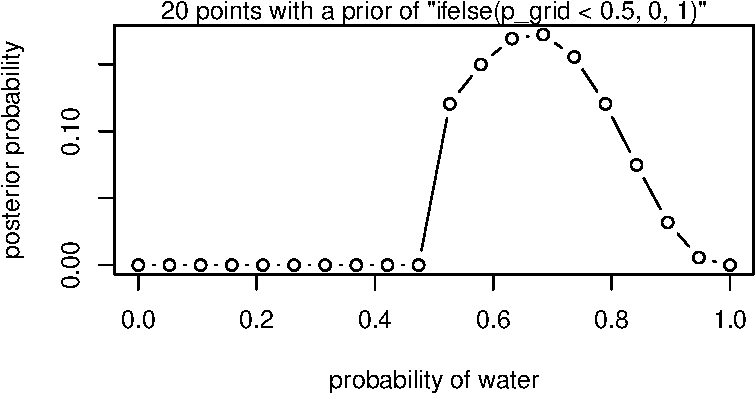
\includegraphics{02-small-and-large-worlds_files/figure-pdf/fig-grid-approx-base2-1.pdf}

}

\caption{\label{fig-grid-approx-base2}Grid Approximation with prior of
\texttt{ifelse(p\_grid\ \textless{}\ 0.5,\ 0,\ 1)}}

\end{figure}

Picture~\ref{fig-grid-approx-base2} employs as prior
\texttt{ifelse(p\_grid\ \textless{}\ 0.5,\ 0,\ 1)}, meaning that if
\texttt{prob} is smaller than 0.5 use zero as prior otherwise 1.

\begin{Shaded}
\begin{Highlighting}[]
\InformationTok{\textasciigrave{}\textasciigrave{}\textasciigrave{}\{r\}}
\CommentTok{\#| label: fig{-}grid{-}approx{-}base3}
\CommentTok{\#| fig{-}cap: "Grid Approximation with prior of \textasciigrave{}exp({-}5 * abs(p\_grid {-} 0.5))\textasciigrave{}"}

\CommentTok{\# 1. define grid}
\NormalTok{p\_grid }\OtherTok{\textless{}{-}} \FunctionTok{seq}\NormalTok{(}\AttributeTok{from =} \DecValTok{0}\NormalTok{, }\AttributeTok{to =} \DecValTok{1}\NormalTok{, }\AttributeTok{length.out =} \DecValTok{20}\NormalTok{)}

\CommentTok{\# 2. define prior}
\NormalTok{prior }\OtherTok{\textless{}{-}} \FunctionTok{exp}\NormalTok{(}\SpecialCharTok{{-}}\DecValTok{5} \SpecialCharTok{*} \FunctionTok{abs}\NormalTok{(p\_grid }\SpecialCharTok{{-}} \FloatTok{0.5}\NormalTok{))}

\CommentTok{\# 3. compute likelihood at each value in grid}
\NormalTok{likelihood }\OtherTok{\textless{}{-}} \FunctionTok{dbinom}\NormalTok{(}\AttributeTok{x =} \DecValTok{6}\NormalTok{, }\AttributeTok{size =} \DecValTok{9}\NormalTok{, }\AttributeTok{prob =}\NormalTok{ p\_grid)}

\CommentTok{\# 4. compute product of likelihood and prior}
\NormalTok{unstd.posterior }\OtherTok{\textless{}{-}}\NormalTok{ likelihood }\SpecialCharTok{*}\NormalTok{ prior}

\CommentTok{\# 5. standardize the posterior, so it sums to 1}
\NormalTok{posterior }\OtherTok{\textless{}{-}}\NormalTok{ unstd.posterior }\SpecialCharTok{/} \FunctionTok{sum}\NormalTok{(unstd.posterior)}

\CommentTok{\# 6 display the posterior distribution }
\DocumentationTok{\#\# R code 2.4}
\FunctionTok{plot}\NormalTok{(p\_grid, posterior,}
  \AttributeTok{type =} \StringTok{"b"}\NormalTok{,}
  \AttributeTok{xlab =} \StringTok{"probability of water"}\NormalTok{, }\AttributeTok{ylab =} \StringTok{"posterior probability"}
\NormalTok{)}
\FunctionTok{mtext}\NormalTok{(}\StringTok{\textquotesingle{}20 points with prior of "exp({-}5 * abs(p\_grid {-} 0.5))"\textquotesingle{}}\NormalTok{)}
\InformationTok{\textasciigrave{}\textasciigrave{}\textasciigrave{}}
\end{Highlighting}
\end{Shaded}

\begin{figure}[H]

{\centering 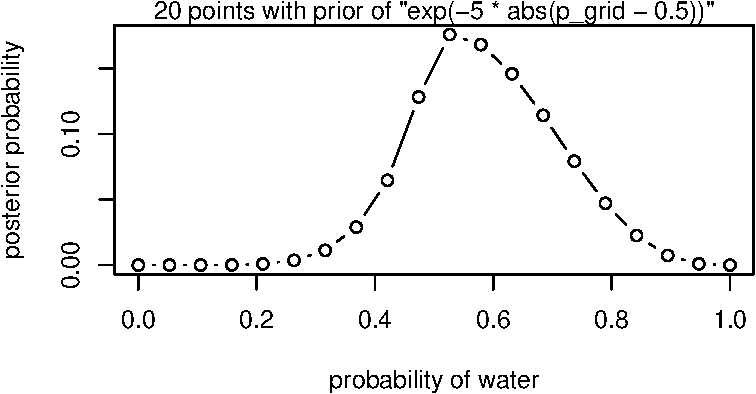
\includegraphics{02-small-and-large-worlds_files/figure-pdf/fig-grid-approx-base3-1.pdf}

}

\caption{\label{fig-grid-approx-base3}Grid Approximation with prior of
\texttt{exp(-5\ *\ abs(p\_grid\ -\ 0.5))}}

\end{figure}

\hypertarget{disadvantage}{%
\paragraph{Disadvantage}\label{disadvantage}}

Grid approximation is very expansive. The number of unique values to
consider in the grid grows rapidly as the number of parameters in the
model increases. For the single-parameter globe tossing model, it's no
problem to compute a grid of 100 or 1000 values. But for two parameters
approximated by 100 values each, that's already 100\textsuperscript{2} =
10.000 values to compute. For 10 parameters, the grid becomes many
billions of values. These days, it's routine to have models with
hundreds or thousands of parameters. The grid approximation strategy
scales very poorly with model complexity, so it won't get us very far.
But it is a very useful didactically as it help to understand the
general principle.

\hypertarget{reconsideration}{%
\subsubsection{Reconsideration}\label{reconsideration}}

\begin{tcolorbox}[enhanced jigsaw, colframe=quarto-callout-caution-color-frame, colback=white, toprule=.15mm, breakable, arc=.35mm, bottomtitle=1mm, colbacktitle=quarto-callout-caution-color!10!white, toptitle=1mm, titlerule=0mm, title=\textcolor{quarto-callout-caution-color}{\faFire}\hspace{0.5em}{Puzzlement}, leftrule=.75mm, opacityback=0, rightrule=.15mm, opacitybacktitle=0.6, bottomrule=.15mm, left=2mm, coltitle=black]

As demonstrated in Picture~\ref{fig-plot-model} a different prior with
the same likelihood has different posteriors. So the curves of all three
examples are different.

But what I do not understand is the fact that in the third example the
result is very different from the other two priors: About 0.5 and not
0.7. My explication: I have only 9 trials. With many more trials the
difference in the density would balance out bit by bit.

But it turns out, that all three show about the same maximum I thought
that the chosen prior did not have any effect the outcome. But it turns
out that different priors results in different PDFs.\\
My explication: I have only 9 trials. With many more trials the
difference in the density would balance out bit by bit.

\end{tcolorbox}

I am going to test my hypothesis. To demonstrate that with more Bayesian
updates we will approach the correct result 0b about 0.7 I will work
with 1000 samples.

\begin{Shaded}
\begin{Highlighting}[]
\InformationTok{\textasciigrave{}\textasciigrave{}\textasciigrave{}\{r\}}
\CommentTok{\#| label: fig{-}grid{-}approx{-}base4}
\CommentTok{\#| fig{-}cap: "Grid Approximation with prior of \textasciigrave{}exp({-}5 * abs(p\_grid {-} 0.5))\textasciigrave{}"}

\CommentTok{\# 1. define grid}
\NormalTok{p\_grid }\OtherTok{\textless{}{-}} \FunctionTok{seq}\NormalTok{(}\AttributeTok{from =} \DecValTok{0}\NormalTok{, }\AttributeTok{to =} \DecValTok{1}\NormalTok{, }\AttributeTok{length.out =} \DecValTok{20}\NormalTok{)}

\CommentTok{\# 2. define prior}
\NormalTok{prior }\OtherTok{\textless{}{-}} \FunctionTok{exp}\NormalTok{(}\SpecialCharTok{{-}}\DecValTok{5} \SpecialCharTok{*} \FunctionTok{abs}\NormalTok{(p\_grid }\SpecialCharTok{{-}} \FloatTok{0.5}\NormalTok{))}

\CommentTok{\# 3. compute likelihood at each value in grid}
\NormalTok{likelihood }\OtherTok{\textless{}{-}} \FunctionTok{dbinom}\NormalTok{(}\AttributeTok{x =} \DecValTok{600}\NormalTok{, }\AttributeTok{size =} \FloatTok{1e3}\NormalTok{, }\AttributeTok{prob =}\NormalTok{ p\_grid)}

\CommentTok{\# 4. compute product of likelihood and prior}
\NormalTok{unstd.posterior }\OtherTok{\textless{}{-}}\NormalTok{ likelihood }\SpecialCharTok{*}\NormalTok{ prior}

\CommentTok{\# 5. standardize the posterior, so it sums to 1}
\NormalTok{posterior }\OtherTok{\textless{}{-}}\NormalTok{ unstd.posterior }\SpecialCharTok{/} \FunctionTok{sum}\NormalTok{(unstd.posterior)}

\CommentTok{\# 6 display the posterior distribution }
\DocumentationTok{\#\# R code 2.4}
\FunctionTok{plot}\NormalTok{(p\_grid, posterior,}
  \AttributeTok{type =} \StringTok{"b"}\NormalTok{,}
  \AttributeTok{xlab =} \StringTok{"probability of water"}\NormalTok{, }\AttributeTok{ylab =} \StringTok{"posterior probability"}
\NormalTok{)}
\FunctionTok{mtext}\NormalTok{(}\StringTok{\textquotesingle{}20 points for a 1000 samples with prior of "exp({-}5 * abs(p\_grid {-} 0.5))"\textquotesingle{}}\NormalTok{)}
\InformationTok{\textasciigrave{}\textasciigrave{}\textasciigrave{}}
\end{Highlighting}
\end{Shaded}

\begin{figure}[H]

{\centering 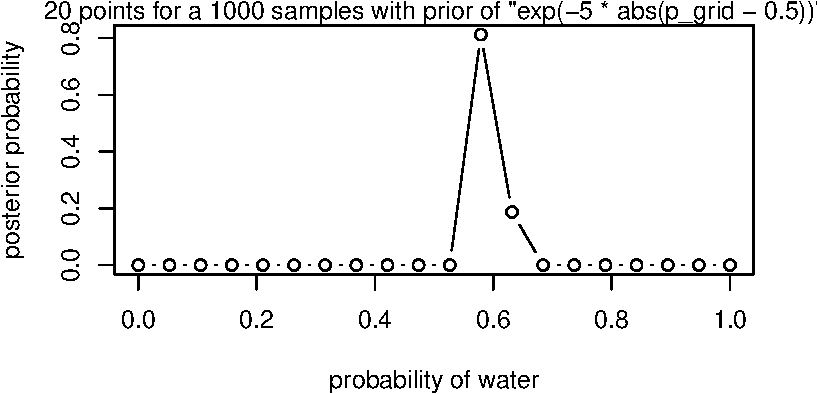
\includegraphics{02-small-and-large-worlds_files/figure-pdf/fig-grid-approx-base4-1.pdf}

}

\caption{\label{fig-grid-approx-base4}Grid Approximation with prior of
\texttt{exp(-5\ *\ abs(p\_grid\ -\ 0.5))}}

\end{figure}

In fact the posterior distribution is nearer to the correct result of
0.7. In Picture~\ref{fig-grid-approx-base3} we have a maximum at about
0.52 and in Picture~\ref{fig-grid-approx-base4} we have already 0.58. We
should also taking into account that with more samples our proportion of
W to L will approach the real Water:Land proportion of about 0.71 too.

I will demonstrate this with 10000 samples and a W:L proportion of 7:3.

\begin{Shaded}
\begin{Highlighting}[]
\InformationTok{\textasciigrave{}\textasciigrave{}\textasciigrave{}\{r\}}
\CommentTok{\#| label: fig{-}grid{-}approx{-}base5}
\CommentTok{\#| fig{-}cap: "Grid Approximation with prior of \textasciigrave{}exp({-}5 * abs(p\_grid {-} 0.5))\textasciigrave{}"}

\CommentTok{\# 1. define grid}
\NormalTok{p\_grid }\OtherTok{\textless{}{-}} \FunctionTok{seq}\NormalTok{(}\AttributeTok{from =} \DecValTok{0}\NormalTok{, }\AttributeTok{to =} \DecValTok{1}\NormalTok{, }\AttributeTok{length.out =} \DecValTok{20}\NormalTok{)}

\CommentTok{\# 2. define prior}
\NormalTok{prior }\OtherTok{\textless{}{-}} \FunctionTok{exp}\NormalTok{(}\SpecialCharTok{{-}}\DecValTok{5} \SpecialCharTok{*} \FunctionTok{abs}\NormalTok{(p\_grid }\SpecialCharTok{{-}} \FloatTok{0.5}\NormalTok{))}

\CommentTok{\# 3. compute likelihood at each value in grid}
\NormalTok{likelihood }\OtherTok{\textless{}{-}} \FunctionTok{dbinom}\NormalTok{(}\AttributeTok{x =} \FloatTok{7e3}\NormalTok{, }\AttributeTok{size =} \FloatTok{1e4}\NormalTok{, }\AttributeTok{prob =}\NormalTok{ p\_grid)}

\CommentTok{\# 4. compute product of likelihood and prior}
\NormalTok{unstd.posterior }\OtherTok{\textless{}{-}}\NormalTok{ likelihood }\SpecialCharTok{*}\NormalTok{ prior}

\CommentTok{\# 5. standardize the posterior, so it sums to 1}
\NormalTok{posterior }\OtherTok{\textless{}{-}}\NormalTok{ unstd.posterior }\SpecialCharTok{/} \FunctionTok{sum}\NormalTok{(unstd.posterior)}

\CommentTok{\# 6 display the posterior distribution }
\DocumentationTok{\#\# R code 2.4}
\FunctionTok{plot}\NormalTok{(p\_grid, posterior,}
  \AttributeTok{type =} \StringTok{"b"}\NormalTok{,}
  \AttributeTok{xlab =} \StringTok{"probability of water"}\NormalTok{, }\AttributeTok{ylab =} \StringTok{"posterior probability"}
\NormalTok{)}
\FunctionTok{mtext}\NormalTok{(}\StringTok{\textquotesingle{}20 points for a 10000 samples with prior of "exp({-}5 * abs(p\_grid {-} 0.5))" and W:L = 7:3.\textquotesingle{}}\NormalTok{ )}
\InformationTok{\textasciigrave{}\textasciigrave{}\textasciigrave{}}
\end{Highlighting}
\end{Shaded}

\begin{figure}[H]

{\centering 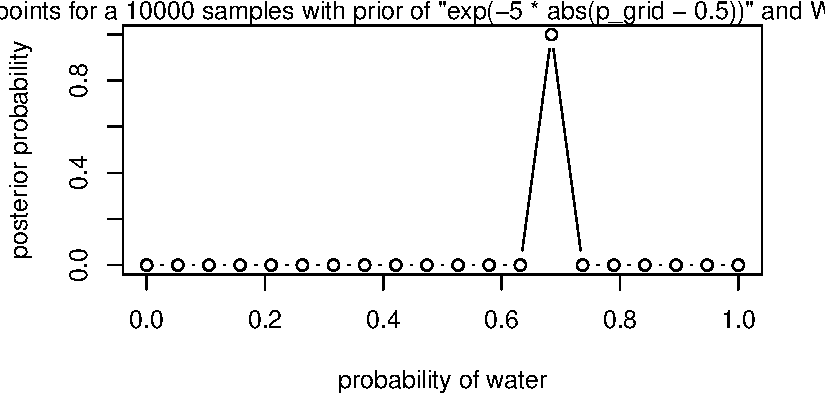
\includegraphics{02-small-and-large-worlds_files/figure-pdf/fig-grid-approx-base5-1.pdf}

}

\caption{\label{fig-grid-approx-base5}Grid Approximation with prior of
\texttt{exp(-5\ *\ abs(p\_grid\ -\ 0.5))}}

\end{figure}

In this example the maximum of probability is already 0.68! We can say
that \textbf{with every chosen prior we will get finally the correct
result!}.

But the choice of the prior is still important as it determines how many
Bayesian updates we need to get the right result. If we have an awkward
prior and not the appropriate size of the sample we will get a posterior
distribution showing us a wrong maximum of probability. In that case the
process of approximation has not reached a state where the probability
maximum is near the correct result. The problem is: Most time we do not
know the correct solution and can't therefore decide if we have had
enough Bayesian updates.

\hypertarget{tidyverse-6}{%
\subsubsection{Tidyverse}\label{tidyverse-6}}

We just employed grid approximation in the Picture~\ref{fig-plot-model}
chunk. To get nice smooth lines, we computed in the
Listing~\ref{lst-prepare-model} chunk the posterior over 1,000
evenly-spaced points on the probability space. Here we'll prepare for
the left panel of Figure 2.7 with just 5 evenly-spaced points.

As a reminder I will add comments for the five steps for the grid
approximation procedure. As it is explained in detail on several other
places I will not produce code annotations.

\hypertarget{produce-grid-data}{%
\paragraph{Produce grid data}\label{produce-grid-data}}

\begin{Shaded}
\begin{Highlighting}[]
\InformationTok{\textasciigrave{}\textasciigrave{}\textasciigrave{}\{r\}}
\CommentTok{\#| label: grid{-}approx1}

\NormalTok{(}
\NormalTok{  d }\OtherTok{\textless{}{-}}
    \CommentTok{\# 1. define grid}
    \FunctionTok{tibble}\NormalTok{(}\AttributeTok{p\_grid =} \FunctionTok{seq}\NormalTok{(}\AttributeTok{from =} \DecValTok{0}\NormalTok{, }\AttributeTok{to =} \DecValTok{1}\NormalTok{, }\AttributeTok{length.out =} \DecValTok{5}\NormalTok{), }
           
    \CommentTok{\# 2. define (compute) prior  }
           \AttributeTok{prior  =} \DecValTok{1}\NormalTok{) }\SpecialCharTok{\%\textgreater{}\%}
        
    \CommentTok{\# 3. compute likelihood at each value in grid}
    \FunctionTok{mutate}\NormalTok{(}\AttributeTok{likelihood =} \FunctionTok{dbinom}\NormalTok{(}\DecValTok{6}\NormalTok{, }\AttributeTok{size =} \DecValTok{9}\NormalTok{, }\AttributeTok{prob =}\NormalTok{ p\_grid)) }\SpecialCharTok{\%\textgreater{}\%} 
        
    \CommentTok{\# 4. compute product of likelihood and prior}
    \FunctionTok{mutate}\NormalTok{(}\AttributeTok{unstd\_posterior =}\NormalTok{ likelihood }\SpecialCharTok{*}\NormalTok{ prior) }\SpecialCharTok{\%\textgreater{}\%}  
        
    \CommentTok{\# 5. standardize the posterior, so it sums to 1}
    \FunctionTok{mutate}\NormalTok{(}\AttributeTok{posterior =}\NormalTok{ unstd\_posterior }\SpecialCharTok{/} \FunctionTok{sum}\NormalTok{(unstd\_posterior))   }
\NormalTok{)}
\InformationTok{\textasciigrave{}\textasciigrave{}\textasciigrave{}}
\end{Highlighting}
\end{Shaded}

\begin{verbatim}
#> # A tibble: 5 x 5
#>   p_grid prior likelihood unstd_posterior posterior
#>    <dbl> <dbl>      <dbl>           <dbl>     <dbl>
#> 1   0        1    0               0          0     
#> 2   0.25     1    0.00865         0.00865    0.0213
#> 3   0.5      1    0.164           0.164      0.404 
#> 4   0.75     1    0.234           0.234      0.575 
#> 5   1        1    0               0          0
\end{verbatim}

\hypertarget{plot-with-only-5-points}{%
\paragraph{Plot with only 5 points}\label{plot-with-only-5-points}}

The next step is to plot the above results to get the left panel of
Figure 2.5

\begin{Shaded}
\begin{Highlighting}[]
\InformationTok{\textasciigrave{}\textasciigrave{}\textasciigrave{}\{r\}}
\CommentTok{\#| label: plot{-}grid{-}approx1}

\NormalTok{p1 }\OtherTok{\textless{}{-}} 
\NormalTok{    d }\SpecialCharTok{|\textgreater{}} 
    \FunctionTok{ggplot}\NormalTok{(}\FunctionTok{aes}\NormalTok{(}\AttributeTok{x =}\NormalTok{ p\_grid, }\AttributeTok{y =}\NormalTok{ posterior)) }\SpecialCharTok{+}
      \FunctionTok{geom\_point}\NormalTok{() }\SpecialCharTok{+}
      \FunctionTok{geom\_line}\NormalTok{() }\SpecialCharTok{+}
      \FunctionTok{labs}\NormalTok{(}\AttributeTok{subtitle =} \StringTok{"5 points"}\NormalTok{,}
           \AttributeTok{x =} \StringTok{"probability of water"}\NormalTok{,}
           \AttributeTok{y =} \StringTok{"posterior probability"}\NormalTok{) }\SpecialCharTok{+}
      \FunctionTok{theme}\NormalTok{(}\AttributeTok{panel.grid =} \FunctionTok{element\_blank}\NormalTok{())}
\NormalTok{p1}
\InformationTok{\textasciigrave{}\textasciigrave{}\textasciigrave{}}
\end{Highlighting}
\end{Shaded}

\begin{figure}[H]

{\centering 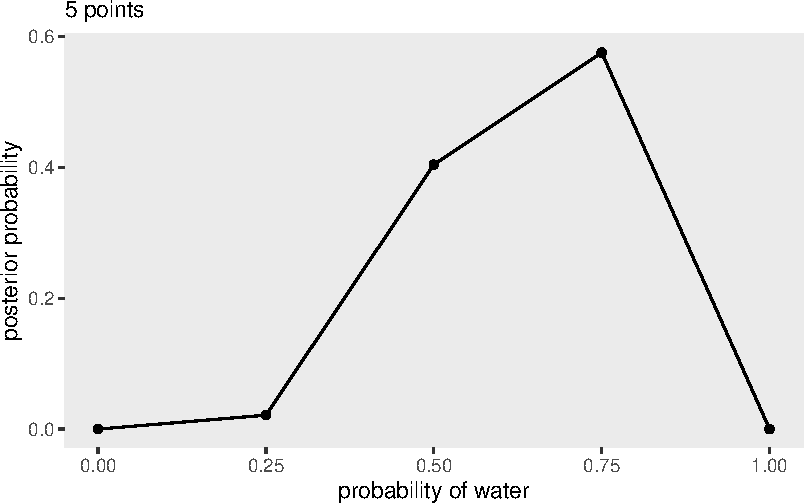
\includegraphics{02-small-and-large-worlds_files/figure-pdf/plot-grid-approx1-1.pdf}

}

\end{figure}

\hypertarget{produce-grid-with-20-points-and-plot-result}{%
\paragraph{Produce grid with 20 points and plot
result}\label{produce-grid-with-20-points-and-plot-result}}

Now the same with 20 evenly spaced points to get the right panel of
Figure 2.7.

\begin{Shaded}
\begin{Highlighting}[]
\InformationTok{\textasciigrave{}\textasciigrave{}\textasciigrave{}\{r\}}
\CommentTok{\#| label: grid{-}approx2}

\NormalTok{p2 }\OtherTok{\textless{}{-}}
  \FunctionTok{tibble}\NormalTok{(}\AttributeTok{p\_grid =} \FunctionTok{seq}\NormalTok{(}\AttributeTok{from =} \DecValTok{0}\NormalTok{, }\AttributeTok{to =} \DecValTok{1}\NormalTok{, }\AttributeTok{length.out =} \DecValTok{20}\NormalTok{),}
         \AttributeTok{prior  =} \DecValTok{1}\NormalTok{) }\SpecialCharTok{\%\textgreater{}\%}
  \FunctionTok{mutate}\NormalTok{(}\AttributeTok{likelihood =} \FunctionTok{dbinom}\NormalTok{(}\DecValTok{6}\NormalTok{, }\AttributeTok{size =} \DecValTok{9}\NormalTok{, }\AttributeTok{prob =}\NormalTok{ p\_grid)) }\SpecialCharTok{\%\textgreater{}\%}
  \FunctionTok{mutate}\NormalTok{(}\AttributeTok{unstd\_posterior =}\NormalTok{ likelihood }\SpecialCharTok{*}\NormalTok{ prior) }\SpecialCharTok{\%\textgreater{}\%}
  \FunctionTok{mutate}\NormalTok{(}\AttributeTok{posterior =}\NormalTok{ unstd\_posterior }\SpecialCharTok{/} \FunctionTok{sum}\NormalTok{(unstd\_posterior)) }\SpecialCharTok{\%\textgreater{}\%} 
  
  \FunctionTok{ggplot}\NormalTok{(}\FunctionTok{aes}\NormalTok{(}\AttributeTok{x =}\NormalTok{ p\_grid, }\AttributeTok{y =}\NormalTok{ posterior)) }\SpecialCharTok{+}
  \FunctionTok{geom\_point}\NormalTok{() }\SpecialCharTok{+}
  \FunctionTok{geom\_line}\NormalTok{() }\SpecialCharTok{+}
  \FunctionTok{labs}\NormalTok{(}\AttributeTok{subtitle =} \StringTok{"20 points"}\NormalTok{,}
       \AttributeTok{x =} \StringTok{"probability of water"}\NormalTok{,}
       \AttributeTok{y =} \StringTok{"posterior probability"}\NormalTok{) }\SpecialCharTok{+}
  \FunctionTok{theme}\NormalTok{(}\AttributeTok{panel.grid =} \FunctionTok{element\_blank}\NormalTok{())}
\NormalTok{p2}
\InformationTok{\textasciigrave{}\textasciigrave{}\textasciigrave{}}
\end{Highlighting}
\end{Shaded}

\begin{figure}[H]

{\centering 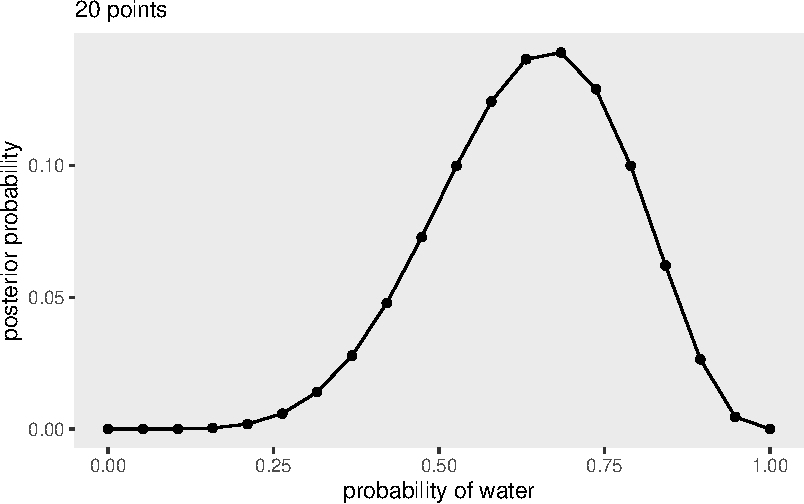
\includegraphics{02-small-and-large-worlds_files/figure-pdf/grid-approx2-1.pdf}

}

\end{figure}

\hypertarget{combine-plots-with-patchwork}{%
\paragraph{Combine plots with
\{patchwork\}}\label{combine-plots-with-patchwork}}

And finally we display the two graphics with the \texttt{+} operator of
\{\textbf{patchwork}\} side by side and annotate the plot with
\texttt{patchwork::plot\_annotation()}.

\begin{Shaded}
\begin{Highlighting}[]
\InformationTok{\textasciigrave{}\textasciigrave{}\textasciigrave{}\{r\}}
\CommentTok{\#| label: plot{-}grid{-}approx{-}b2}

\CommentTok{\# needs library(patchwork) = defined in setup chunk}
\NormalTok{p1 }\SpecialCharTok{+}\NormalTok{ p2 }\SpecialCharTok{+} \FunctionTok{plot\_annotation}\NormalTok{(}\AttributeTok{title =} \StringTok{"More grid points make for smoother approximations"}\NormalTok{)}
\InformationTok{\textasciigrave{}\textasciigrave{}\textasciigrave{}}
\end{Highlighting}
\end{Shaded}

\begin{figure}[H]

{\centering 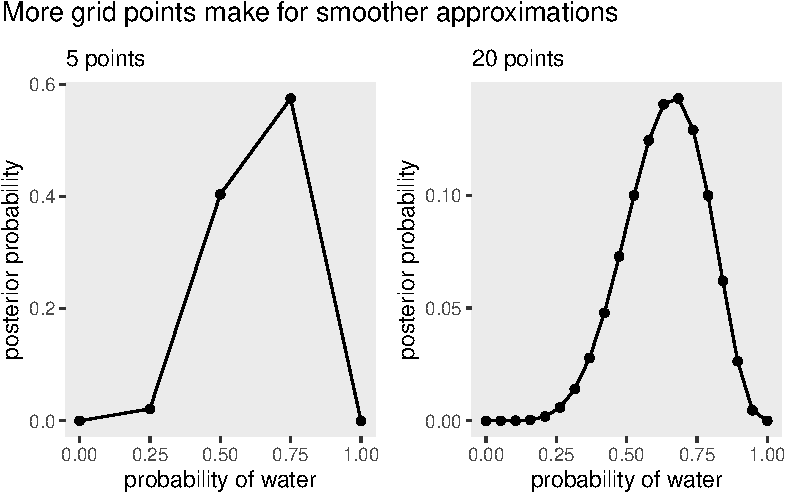
\includegraphics{02-small-and-large-worlds_files/figure-pdf/plot-grid-approx-b2-1.pdf}

}

\end{figure}

\hypertarget{using-differnt-prior-functions}{%
\paragraph{Using differnt prior
functions}\label{using-differnt-prior-functions}}

To see the influence of the prior probability on the posterior
probability by using the same likelihood the book offers two code
snippets. Replace the definition of the prior (number 2 in the code
snippet) --- one at a time --- with the following lines of code:

\begin{Shaded}
\begin{Highlighting}[]
\InformationTok{\textasciigrave{}\textasciigrave{}\textasciigrave{}\{r\}}
\CommentTok{\#| label: lst{-}different{-}priors}
\CommentTok{\#| lst{-}cap: "Two other prior functions to try out what happens with different priors."}

\NormalTok{prior }\OtherTok{\textless{}{-}} \FunctionTok{ifelse}\NormalTok{(p\_grid }\SpecialCharTok{\textless{}} \FloatTok{0.5}\NormalTok{, }\DecValTok{0}\NormalTok{, }\DecValTok{1}\NormalTok{)}
\NormalTok{prior }\OtherTok{\textless{}{-}} \FunctionTok{exp}\NormalTok{(}\SpecialCharTok{{-}}\DecValTok{5} \SpecialCharTok{*} \FunctionTok{abs}\NormalTok{(p\_grid }\SpecialCharTok{{-}} \FloatTok{0.5}\NormalTok{))}
\InformationTok{\textasciigrave{}\textasciigrave{}\textasciigrave{}}
\end{Highlighting}
\end{Shaded}

What follows is a condensed way to make the four plots all at once. It
is a pretty complex program snippet not only using
\texttt{tidyr::expand\_grid()} --- as already explained ---, but also
\texttt{tidyr::unnest()} which expands a list-column containing data
frames into rows and columns.

\begin{Shaded}
\begin{Highlighting}[]
\InformationTok{\textasciigrave{}\textasciigrave{}\textasciigrave{}\{r\}}
\CommentTok{\#| label: fig{-}different{-}priors{-}5{-}and{-}20{-}points}
\CommentTok{\#| fig{-}cap: "The effect of different priors and of different amounts of grid points."}


\CommentTok{\# prepare the plot by producing the data}
\FunctionTok{tibble}\NormalTok{(}\AttributeTok{n\_points =} \FunctionTok{c}\NormalTok{(}\DecValTok{5}\NormalTok{, }\DecValTok{20}\NormalTok{)) }\SpecialCharTok{\%\textgreater{}\%} 
  \FunctionTok{mutate}\NormalTok{(}\AttributeTok{p\_grid =}\NormalTok{ purrr}\SpecialCharTok{::}\FunctionTok{map}\NormalTok{(n\_points, }\SpecialCharTok{\textasciitilde{}}\FunctionTok{seq}\NormalTok{(}\AttributeTok{from =} \DecValTok{0}\NormalTok{, }\AttributeTok{to =} \DecValTok{1}\NormalTok{, }\AttributeTok{length.out =}\NormalTok{ .))) }\SpecialCharTok{\%\textgreater{}\%} 
  \FunctionTok{unnest}\NormalTok{(p\_grid) }\SpecialCharTok{\%\textgreater{}\%} 
  \FunctionTok{expand\_grid}\NormalTok{(}\AttributeTok{priors =} \FunctionTok{c}\NormalTok{(}\StringTok{"ifelse(p\_grid \textless{} 0.5, 0, 1)"}\NormalTok{, }\StringTok{"exp({-}5 * abs(p\_grid {-} 0.5))"}\NormalTok{)) }\SpecialCharTok{\%\textgreater{}\%} 
  \FunctionTok{mutate}\NormalTok{(}\AttributeTok{prior =} \FunctionTok{ifelse}\NormalTok{(priors }\SpecialCharTok{==} \StringTok{"ifelse(p\_grid \textless{} 0.5, 0, 1)"}\NormalTok{, }
                        \FunctionTok{ifelse}\NormalTok{(p\_grid }\SpecialCharTok{\textless{}} \FloatTok{0.5}\NormalTok{, }\DecValTok{0}\NormalTok{, }\DecValTok{1}\NormalTok{),}
                        \FunctionTok{exp}\NormalTok{(}\SpecialCharTok{{-}}\DecValTok{5} \SpecialCharTok{*} \FunctionTok{abs}\NormalTok{(p\_grid }\SpecialCharTok{{-}} \FloatTok{0.5}\NormalTok{)))) }\SpecialCharTok{\%\textgreater{}\%} 
  \FunctionTok{mutate}\NormalTok{(}\AttributeTok{likelihood =} \FunctionTok{dbinom}\NormalTok{(}\DecValTok{6}\NormalTok{, }\AttributeTok{size =} \DecValTok{9}\NormalTok{, }\AttributeTok{prob =}\NormalTok{ p\_grid)) }\SpecialCharTok{\%\textgreater{}\%} 
  \FunctionTok{mutate}\NormalTok{(}\AttributeTok{posterior =}\NormalTok{ likelihood }\SpecialCharTok{*}\NormalTok{ prior }\SpecialCharTok{/} \FunctionTok{sum}\NormalTok{(likelihood }\SpecialCharTok{*}\NormalTok{ prior)) }\SpecialCharTok{\%\textgreater{}\%} 
  \FunctionTok{mutate}\NormalTok{(}\AttributeTok{n\_points =} \FunctionTok{str\_c}\NormalTok{(}\StringTok{"\# points = "}\NormalTok{, n\_points),}
         \AttributeTok{priors   =} \FunctionTok{str\_c}\NormalTok{(}\StringTok{"prior = "}\NormalTok{, priors)) }\SpecialCharTok{\%\textgreater{}\%} 
  
  \CommentTok{\# plot the data}
  \FunctionTok{ggplot}\NormalTok{(}\FunctionTok{aes}\NormalTok{(}\AttributeTok{x =}\NormalTok{ p\_grid, }\AttributeTok{y =}\NormalTok{ posterior)) }\SpecialCharTok{+}
  \FunctionTok{geom\_line}\NormalTok{() }\SpecialCharTok{+}
  \FunctionTok{geom\_point}\NormalTok{() }\SpecialCharTok{+}
  \FunctionTok{labs}\NormalTok{(}\AttributeTok{x =} \StringTok{"probability of water"}\NormalTok{,}
       \AttributeTok{y =} \StringTok{"posterior probability"}\NormalTok{) }\SpecialCharTok{+}
  \FunctionTok{theme}\NormalTok{(}\AttributeTok{panel.grid =} \FunctionTok{element\_blank}\NormalTok{()) }\SpecialCharTok{+}
  \FunctionTok{facet\_grid}\NormalTok{(n\_points }\SpecialCharTok{\textasciitilde{}}\NormalTok{ priors, }\AttributeTok{scales =} \StringTok{"free"}\NormalTok{)}
\InformationTok{\textasciigrave{}\textasciigrave{}\textasciigrave{}}
\end{Highlighting}
\end{Shaded}

\begin{figure}[H]

{\centering 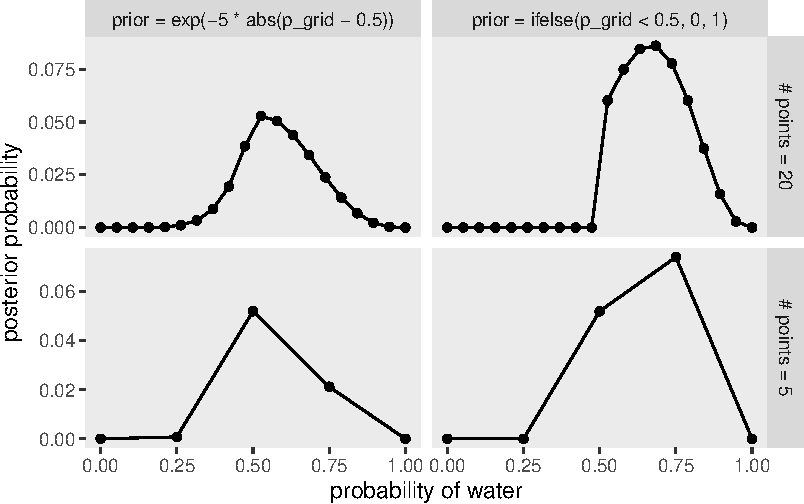
\includegraphics{02-small-and-large-worlds_files/figure-pdf/fig-different-priors-5-and-20-points-1.pdf}

}

\caption{\label{fig-different-priors-5-and-20-points}The effect of
different priors and of different amounts of grid points.}

\end{figure}

\hypertarget{quadratic-approximation}{%
\subsection{Quadratic Approximation}\label{quadratic-approximation}}

\hypertarget{original-7}{%
\subsubsection{Original}\label{original-7}}

\hypertarget{concept}{%
\paragraph{Concept}\label{concept}}

\begin{quote}
Under quite general conditions, the region near the peak of the
posterior distribution will be nearly Gaussian---or ``normal''---in
shape. This means the posterior distribution can be usefully
approximated by a Gaussian distribution. A Gaussian distribution is
convenient, because it can be completely described by only two numbers:
the location of its center (mean) and its spread (variance).
\end{quote}

\begin{quote}
A Gaussian approximation is called ``quadratic approximation'' because
the logarithm of a Gaussian distribution forms a parabola. And a
parabola is a quadratic function.
\end{quote}

Two steps: 1. Find the posterior mode with some algorithm. The procedure
does not know where the peak is but it knows the slope under it feet. 2.
Estimate the curvature near the peak to calculate a quadratic
approximation. This computation is done by some numerical technique.

\hypertarget{computing-the-quadratic-approximation}{%
\paragraph{Computing the quadratic
approximation}\label{computing-the-quadratic-approximation}}

To compute the quadratic approximation for the globe tossing data, we'll
use a tool in the \{\textbf{rethinking}\} package:
\texttt{rethinking::quap()}.

\begin{Shaded}
\begin{Highlighting}[]
\InformationTok{\textasciigrave{}\textasciigrave{}\textasciigrave{}\{r\}}
\CommentTok{\#| label: quadratic{-}approx{-}9}

\NormalTok{globe.qa }\OtherTok{\textless{}{-}}\NormalTok{ rethinking}\SpecialCharTok{::}\FunctionTok{quap}\NormalTok{(}
  \FunctionTok{alist}\NormalTok{(}
\NormalTok{    W }\SpecialCharTok{\textasciitilde{}} \FunctionTok{dbinom}\NormalTok{(W }\SpecialCharTok{+}\NormalTok{ L, p), }\CommentTok{\# binomial likelihood}
\NormalTok{    p }\SpecialCharTok{\textasciitilde{}} \FunctionTok{dunif}\NormalTok{(}\DecValTok{0}\NormalTok{, }\DecValTok{1}\NormalTok{) }\CommentTok{\# uniform prior}
\NormalTok{  ),}
  \AttributeTok{data =} \FunctionTok{list}\NormalTok{(}\AttributeTok{W =} \DecValTok{6}\NormalTok{, }\AttributeTok{L =} \DecValTok{3}\NormalTok{)}
\NormalTok{)}

\CommentTok{\# display summary of quadratic approximation}
\NormalTok{rethinking}\SpecialCharTok{::}\FunctionTok{precis}\NormalTok{(globe.qa)}
\InformationTok{\textasciigrave{}\textasciigrave{}\textasciigrave{}}
\end{Highlighting}
\end{Shaded}

\begin{verbatim}
#>        mean        sd      5.5%     94.5%
#> p 0.6666667 0.1571338 0.4155365 0.9177968
\end{verbatim}

\begin{tcolorbox}[enhanced jigsaw, colframe=quarto-callout-warning-color-frame, colback=white, toprule=.15mm, breakable, arc=.35mm, bottomtitle=1mm, colbacktitle=quarto-callout-warning-color!10!white, toptitle=1mm, titlerule=0mm, title=\textcolor{quarto-callout-warning-color}{\faExclamationTriangle}\hspace{0.5em}{\texttt{precis()} results not printed correctly from visual mode}, leftrule=.75mm, opacityback=0, rightrule=.15mm, opacitybacktitle=0.6, bottomrule=.15mm, left=2mm, coltitle=black]

The result of \texttt{rethinking::precis()} does not display correctly
after the chunk in RStudio visual mode. But it works in source mode and
it displayed correctly immediately after the chunk.

The columns of the table are too narrow so that you can't see the header
and inspect the values. Printing to the console or to the web is
correct.

A workaround is wrapping the result with \texttt{print()} or to render
the document in source mode. See my
\href{https://github.com/rstudio/rstudio/issues/13227}{bug report}.

\end{tcolorbox}

To use \texttt{quap()}, you provide a \emph{formula}, a list of
\emph{data} with \texttt{base::alist()}. \texttt{alist()} handles its
arguments as if they described function arguments. So the values are not
evaluated, and tagged arguments with no value are allowed. It is most
often used in conjunction with \texttt{base::formals()}.

The function \texttt{precis} presents a brief summary of the quadratic
approximation. In this case, it shows the posterior mean value of
\(p = 0.67\), which it calls the ``Mean.'' The curvature is labeled
``StdDev''. This stands for \emph{standard deviation}. This value is the
standard deviation of the posterior distribution, while the mean value
is its peak. Finally, the last two values in the \texttt{precis} output
show the 89\% percentile interval, which you'll learn more about in the
next chapter. You can read this kind of approximation like:
\emph{Assuming the posterior is Gaussian, it is maximized at 0.67, and
its standard deviation is 0.16}.

\hypertarget{computing-analytical-solution}{%
\paragraph{Computing analytical
solution}\label{computing-analytical-solution}}

We want to compare the quadratic approximation with the analytic
calculation.

\begin{Shaded}
\begin{Highlighting}[]
\InformationTok{\textasciigrave{}\textasciigrave{}\textasciigrave{}\{r\}}
\CommentTok{\#| label: analytical{-}calc}

\CommentTok{\# analytic calculation}
\NormalTok{W }\OtherTok{\textless{}{-}} \DecValTok{6}
\NormalTok{L }\OtherTok{\textless{}{-}} \DecValTok{3}
\FunctionTok{curve}\NormalTok{(}\FunctionTok{dbeta}\NormalTok{(x, W }\SpecialCharTok{+} \DecValTok{1}\NormalTok{, L }\SpecialCharTok{+} \DecValTok{1}\NormalTok{), }\AttributeTok{from =} \DecValTok{0}\NormalTok{, }\AttributeTok{to =} \DecValTok{1}\NormalTok{)}

\CommentTok{\# quadratic approximation}
\FunctionTok{curve}\NormalTok{(}\FunctionTok{dnorm}\NormalTok{(x, }\FloatTok{0.67}\NormalTok{, }\FloatTok{0.16}\NormalTok{), }\AttributeTok{lty =} \DecValTok{2}\NormalTok{, }\AttributeTok{add =} \ConstantTok{TRUE}\NormalTok{)}
\InformationTok{\textasciigrave{}\textasciigrave{}\textasciigrave{}}
\end{Highlighting}
\end{Shaded}

\begin{figure}[H]

{\centering 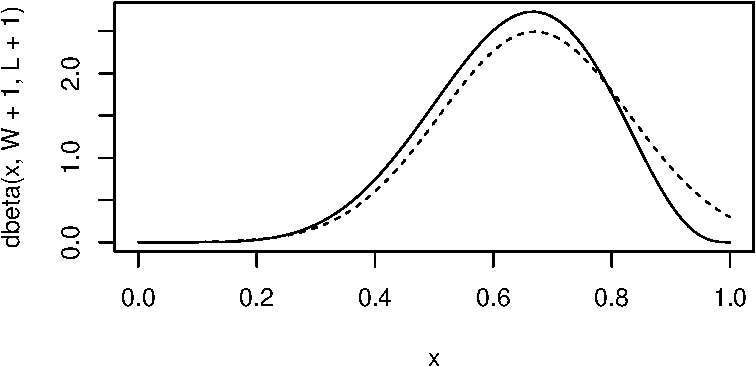
\includegraphics{02-small-and-large-worlds_files/figure-pdf/analytical-calc-1.pdf}

}

\end{figure}

The solid line curve is the analytical posterior and the dashed curve is
the quadratic approximation. The dashed curve does alright on its left
side, but looks pretty bad on its right side. It even assigns positive
probability to \(p = 1\), which we know is impossible, since we saw at
least one land sample. As the amount of data increases, however, the
quadratic approximation gets better.

\hypertarget{disadvantage-1}{%
\paragraph{Disadvantage}\label{disadvantage-1}}

The phenomenon, where the quadratic approximation improves with the
amount of data, is very common. It's one of the reasons that so many
classical statistical procedures are nervous about small samples.

Using the quadratic approximation in a Bayesian context brings with it
all the same concerns. But you can always lean on some algorithm other
than quadratic approximation, if you have doubts. Indeed, grid
approximation works very well with small samples, because in such cases
the model must be simple and the computations will be quite fast. You
can also use MCMC.

Sometimes the quadratic approximation fails and you will get an error
message about the ``Hessian''. A \emph{Hessian} --- named after
mathematician Ludwig Otto Hesse (1811--1874) --- is a square matrix of
second derivatives. The standard deviation is typically computed from
the Hessian, so computing the Hessian is nearly always a necessary step.
But sometimes the computation goes wrong, and your golem will choke
while trying to compute the Hessian.

Some other drawbacks will be explicated in later chapter. Therefore MCMC
seems generally the best option for complex models.

\hypertarget{tidyverse-7}{%
\subsubsection{Tidyverse}\label{tidyverse-7}}

\hypertarget{quadratic-approximation-with-different-sample-size}{%
\paragraph{Quadratic approximation with different sample
size}\label{quadratic-approximation-with-different-sample-size}}

In the book the calculation is only done for \(n = 9\) but McElreath
also display the graphs for \(n = 18\) and \(n = 36\) with the same
proportion of \texttt{W} and \texttt{L}. Kurz shows how this is done and
results into Figure 2.8 in the book.

\begin{codelisting}

\caption{Quadratic approximation with quap() showing the effect of
different sample size}

\hypertarget{lst-quap-different-sample-size}{%
\label{lst-quap-different-sample-size}}%
\begin{Shaded}
\begin{Highlighting}[]
\InformationTok{\textasciigrave{}\textasciigrave{}\textasciigrave{}\{r\}}
\CommentTok{\#| label: quap{-}different{-}sample{-}size}
\CommentTok{\#| attr{-}source: \textquotesingle{}\#lst{-}quap{-}different{-}sample{-}size lst{-}cap="Quadratic approximation with quap() showing the effect of different sample size"\textquotesingle{}}

\DocumentationTok{\#\#\# quap() with 9 sample size \#\#\#\#\#\#\#\#\#\#\#\#\#\#\#\#\#\#\#\#\#\#\#\#\#\#\#\#\#\#\#\#\#}
\NormalTok{globe\_qa\_9 }\OtherTok{\textless{}{-}}\NormalTok{ rethinking}\SpecialCharTok{::}\FunctionTok{quap}\NormalTok{(}
  \FunctionTok{alist}\NormalTok{(}
\NormalTok{    W }\SpecialCharTok{\textasciitilde{}} \FunctionTok{dbinom}\NormalTok{(W }\SpecialCharTok{+}\NormalTok{ L, p), }\CommentTok{\# binomial likelihood}
\NormalTok{    p }\SpecialCharTok{\textasciitilde{}} \FunctionTok{dunif}\NormalTok{(}\DecValTok{0}\NormalTok{, }\DecValTok{1}\NormalTok{) }\CommentTok{\# uniform prior}
\NormalTok{  ),}
  \AttributeTok{data =} \FunctionTok{list}\NormalTok{(}\AttributeTok{W =} \DecValTok{6}\NormalTok{, }\AttributeTok{L =} \DecValTok{3}\NormalTok{)}
\NormalTok{)}

\CommentTok{\# display summary of quadratic approximation}
\NormalTok{rethinking}\SpecialCharTok{::}\FunctionTok{precis}\NormalTok{(globe\_qa\_9)}

\DocumentationTok{\#\#\# quap() with 18 sample size \#\#\#\#\#\#\#\#\#\#\#\#\#\#\#\#\#\#\#\#\#\#\#\#\#\#\#\#\#\#\#\#\#\#\#}
\NormalTok{globe\_qa\_18 }\OtherTok{\textless{}{-}}\NormalTok{ rethinking}\SpecialCharTok{::}\FunctionTok{quap}\NormalTok{(}
  \FunctionTok{alist}\NormalTok{(}
\NormalTok{    W }\SpecialCharTok{\textasciitilde{}} \FunctionTok{dbinom}\NormalTok{(W }\SpecialCharTok{+}\NormalTok{ L, p), }\CommentTok{\# binomial likelihood}
\NormalTok{    p }\SpecialCharTok{\textasciitilde{}} \FunctionTok{dunif}\NormalTok{(}\DecValTok{0}\NormalTok{, }\DecValTok{1}\NormalTok{) }\CommentTok{\# uniform prior}
\NormalTok{  ),}
  \AttributeTok{data =} \FunctionTok{list}\NormalTok{(}\AttributeTok{W =} \DecValTok{12}\NormalTok{, }\AttributeTok{L =} \DecValTok{6}\NormalTok{)}
\NormalTok{)}

\CommentTok{\# display summary of quadratic approximation}
\NormalTok{rethinking}\SpecialCharTok{::}\FunctionTok{precis}\NormalTok{(globe\_qa\_18)}

\DocumentationTok{\#\#\# quap() with 36 sample size \#\#\#\#\#\#\#\#\#\#\#\#\#\#\#\#\#\#\#\#\#\#\#\#\#\#\#\#\#\#\#\#\#\#\#}
\NormalTok{globe\_qa\_36 }\OtherTok{\textless{}{-}}\NormalTok{ rethinking}\SpecialCharTok{::}\FunctionTok{quap}\NormalTok{(}
  \FunctionTok{alist}\NormalTok{(}
\NormalTok{    W }\SpecialCharTok{\textasciitilde{}} \FunctionTok{dbinom}\NormalTok{(W }\SpecialCharTok{+}\NormalTok{ L, p), }\CommentTok{\# binomial likelihood}
\NormalTok{    p }\SpecialCharTok{\textasciitilde{}} \FunctionTok{dunif}\NormalTok{(}\DecValTok{0}\NormalTok{, }\DecValTok{1}\NormalTok{) }\CommentTok{\# uniform prior}
\NormalTok{  ),}
  \AttributeTok{data =} \FunctionTok{list}\NormalTok{(}\AttributeTok{W =} \DecValTok{24}\NormalTok{, }\AttributeTok{L =} \DecValTok{12}\NormalTok{)}
\NormalTok{)}

\CommentTok{\# display summary of quadratic approximation}
\NormalTok{rethinking}\SpecialCharTok{::}\FunctionTok{precis}\NormalTok{(globe\_qa\_36)}
\InformationTok{\textasciigrave{}\textasciigrave{}\textasciigrave{}}
\end{Highlighting}
\end{Shaded}

\end{codelisting}

\begin{verbatim}
#>       mean        sd      5.5%     94.5%
#> p 0.666668 0.1571335 0.4155384 0.9177976
#>        mean        sd      5.5%     94.5%
#> p 0.6666662 0.1111104 0.4890903 0.8442421
#>       mean         sd     5.5%    94.5%
#> p 0.666667 0.07856685 0.541102 0.792232
\end{verbatim}

\begin{tcolorbox}[enhanced jigsaw, colframe=quarto-callout-note-color-frame, colback=white, toprule=.15mm, breakable, arc=.35mm, bottomtitle=1mm, colbacktitle=quarto-callout-note-color!10!white, toptitle=1mm, titlerule=0mm, title=\textcolor{quarto-callout-note-color}{\faInfo}\hspace{0.5em}{Slightly different code}, leftrule=.75mm, opacityback=0, rightrule=.15mm, opacitybacktitle=0.6, bottomrule=.15mm, left=2mm, coltitle=black]

I used a slightly different code than Kurz. I have only changed the data
values.

\end{tcolorbox}

\begin{codelisting}

\caption{Accuracy of the quadratic approximation}

\hypertarget{lst-fig-quadratic-approx}{%
\label{lst-fig-quadratic-approx}}%
\begin{Shaded}
\begin{Highlighting}[]
\InformationTok{\textasciigrave{}\textasciigrave{}\textasciigrave{}\{r\}}
\CommentTok{\#| label: fig{-}quadratic{-}approx}
\CommentTok{\#| fig{-}cap: "Accuracy of the quadratic approximation. In each plot, the exact posterior distribution is plotted as solid curve, and the quadratic approximation is plotted as the dashed curve."}
\CommentTok{\#| attr{-}source: \textquotesingle{}\#lst{-}fig{-}quadratic{-}approx lst{-}cap="Accuracy of the quadratic approximation"\textquotesingle{}}

\NormalTok{n\_grid }\OtherTok{\textless{}{-}} \DecValTok{100}

\CommentTok{\# wrangle}
\FunctionTok{tibble}\NormalTok{(}\AttributeTok{w =} \FunctionTok{c}\NormalTok{(}\DecValTok{6}\NormalTok{, }\DecValTok{12}\NormalTok{, }\DecValTok{24}\NormalTok{),}
       \AttributeTok{n =} \FunctionTok{c}\NormalTok{(}\DecValTok{9}\NormalTok{, }\DecValTok{18}\NormalTok{, }\DecValTok{36}\NormalTok{),}
       \AttributeTok{s =} \FunctionTok{c}\NormalTok{(.}\DecValTok{16}\NormalTok{, .}\DecValTok{11}\NormalTok{, .}\DecValTok{08}\NormalTok{)) }\SpecialCharTok{\%\textgreater{}\%} 
  \FunctionTok{expand\_grid}\NormalTok{(}\AttributeTok{p\_grid =} \FunctionTok{seq}\NormalTok{(}\AttributeTok{from =} \DecValTok{0}\NormalTok{, }\AttributeTok{to =} \DecValTok{1}\NormalTok{, }\AttributeTok{length.out =}\NormalTok{ n\_grid)) }\SpecialCharTok{\%\textgreater{}\%} 
  \FunctionTok{mutate}\NormalTok{(}\AttributeTok{prior =} \DecValTok{1}\NormalTok{,}
         \AttributeTok{m     =}\NormalTok{ .}\DecValTok{67}\NormalTok{)  }\SpecialCharTok{\%\textgreater{}\%}
  \FunctionTok{mutate}\NormalTok{(}\AttributeTok{likelihood =} \FunctionTok{dbinom}\NormalTok{(w, }\AttributeTok{size =}\NormalTok{ n, }\AttributeTok{prob =}\NormalTok{ p\_grid)) }\SpecialCharTok{\%\textgreater{}\%}
  \FunctionTok{mutate}\NormalTok{(}\AttributeTok{unstd\_grid\_posterior =}\NormalTok{ likelihood }\SpecialCharTok{*}\NormalTok{ prior,}
         \AttributeTok{unstd\_quad\_posterior =} \FunctionTok{dnorm}\NormalTok{(p\_grid, m, s)) }\SpecialCharTok{\%\textgreater{}\%}
  \FunctionTok{group\_by}\NormalTok{(w) }\SpecialCharTok{\%\textgreater{}\%} 
  \FunctionTok{mutate}\NormalTok{(}\AttributeTok{grid\_posterior =}\NormalTok{ unstd\_grid\_posterior }\SpecialCharTok{/} \FunctionTok{sum}\NormalTok{(unstd\_grid\_posterior),}
         \AttributeTok{quad\_posterior =}\NormalTok{ unstd\_quad\_posterior }\SpecialCharTok{/} \FunctionTok{sum}\NormalTok{(unstd\_quad\_posterior),}
         \AttributeTok{n              =} \FunctionTok{str\_c}\NormalTok{(}\StringTok{"n = "}\NormalTok{, n)) }\SpecialCharTok{\%\textgreater{}\%} 
  \FunctionTok{mutate}\NormalTok{(}\AttributeTok{n =} \FunctionTok{factor}\NormalTok{(n, }\AttributeTok{levels =} \FunctionTok{c}\NormalTok{(}\StringTok{"n = 9"}\NormalTok{, }\StringTok{"n = 18"}\NormalTok{, }\StringTok{"n = 36"}\NormalTok{))) }\SpecialCharTok{\%\textgreater{}\%} 
  
  \CommentTok{\# plot}
  \FunctionTok{ggplot}\NormalTok{(}\FunctionTok{aes}\NormalTok{(}\AttributeTok{x =}\NormalTok{ p\_grid)) }\SpecialCharTok{+}
  \FunctionTok{geom\_line}\NormalTok{(}\FunctionTok{aes}\NormalTok{(}\AttributeTok{y =}\NormalTok{ grid\_posterior)) }\SpecialCharTok{+}
  \FunctionTok{geom\_line}\NormalTok{(}\FunctionTok{aes}\NormalTok{(}\AttributeTok{y =}\NormalTok{ quad\_posterior),}
            \AttributeTok{color =} \StringTok{"grey50"}\NormalTok{) }\SpecialCharTok{+}
  \FunctionTok{labs}\NormalTok{(}\AttributeTok{x =} \StringTok{"proportion water"}\NormalTok{,}
       \AttributeTok{y =} \StringTok{"density"}\NormalTok{) }\SpecialCharTok{+}
  \FunctionTok{theme}\NormalTok{(}\AttributeTok{panel.grid =} \FunctionTok{element\_blank}\NormalTok{()) }\SpecialCharTok{+}
  \FunctionTok{facet\_wrap}\NormalTok{(}\SpecialCharTok{\textasciitilde{}}\NormalTok{ n, }\AttributeTok{scales =} \StringTok{"free"}\NormalTok{)}
\InformationTok{\textasciigrave{}\textasciigrave{}\textasciigrave{}}
\end{Highlighting}
\end{Shaded}

\end{codelisting}

\begin{figure}[H]

{\centering 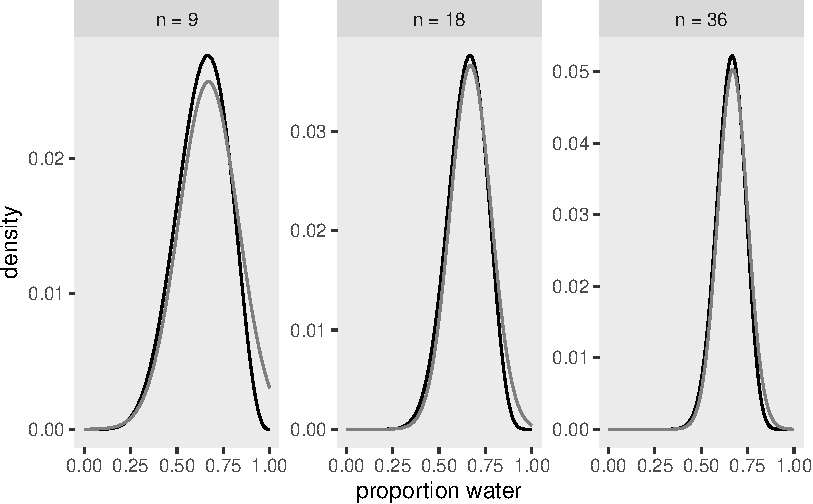
\includegraphics{02-small-and-large-worlds_files/figure-pdf/fig-quadratic-approx-1.pdf}

}

\caption{\label{fig-quadratic-approx}Accuracy of the quadratic
approximation. In each plot, the exact posterior distribution is plotted
as solid curve, and the quadratic approximation is plotted as the dashed
curve.}

\end{figure}

\hypertarget{maximum-likelihood-estimation-mle}{%
\paragraph{Maximum Likelihood Estimation
(MLE)}\label{maximum-likelihood-estimation-mle}}

\begin{quote}
The quadratic approximation, either with a uniform prior or with a lot
of data, is often equivalent to a maximum likelihood estimate (MLE) and
its standard error. The MLE is a very common non-Bayesian parameter
estimate. This correspondence between a Bayesian approximation and a
common non-Bayesian estimator is both a blessing and a curse. It is a
blessing, because it allows us to re-interpret a wide range of published
non-Bayesian model fits in Bayesian terms. It is a curse, because
maximum likelihood estimates have some curious drawbacks, and the
quadratic approximation can share them. (p.~44, emphasis, in the
original)
\end{quote}

Textbooks highlighting the maximum likelihood method for the generalized
linear model abound. If this is new to you and you'd like to learn more,
perhaps check out Roback and Legler's (2021) Beyond multiple linear
regression: Applied generalized linear models and multilevel models in
R, Agresti's (2015) Foundations of linear and generalized linear models
or Dunn and Smyth's (2018) Generalized linear models with examples in R.

\hypertarget{markov-chain-monte-carlo-mcmc}{%
\subsection{Markov Chain Monte Carlo
(MCMC)}\label{markov-chain-monte-carlo-mcmc}}

\hypertarget{original-8}{%
\subsubsection{Original}\label{original-8}}

\begin{quote}
There are lots of important model types, like multilevel (mixed-effects)
models, for which neither grid approximation nor quadratic approximation
is always satisfactory. \ldots{} As a result, various counterintuitive
model fitting techniques have arisen. The most popular of these is
\textbf{MARKOV CHAIN MONTE CARLO} (MCMC), which is a family of
conditioning engines capable of handling highly complex models.
\end{quote}

\begin{quote}
Instead of attempting to compute or approximate the posterior
distribution directly, MCMC techniques merely draw samples from the
posterior. You end up with a collection of parameter values, and the
frequencies of these values correspond to the posterior plausibilities.
You can then build a picture of the posterior from the histogram of
these samples.
\end{quote}

The understanding of this not intuitive technique is postponed to
chapter 9. What follows is just a demonstration of the technique.

\begin{Shaded}
\begin{Highlighting}[]
\InformationTok{\textasciigrave{}\textasciigrave{}\textasciigrave{}\{r\}}
\CommentTok{\#| label: fig{-}demo{-}MCMC{-}rethinking}
\CommentTok{\#| fig{-}cap: "Demo of the Markov Chain Monte Carlo (MCMC) method using the globe{-}tossing data and calculated and diplayed with the \{**rethinking**\} package."}

\DocumentationTok{\#\# R code 2.8}
\NormalTok{n\_samples }\OtherTok{\textless{}{-}} \DecValTok{1000}
\NormalTok{p }\OtherTok{\textless{}{-}} \FunctionTok{rep}\NormalTok{(}\ConstantTok{NA}\NormalTok{, n\_samples)}
\NormalTok{p[}\DecValTok{1}\NormalTok{] }\OtherTok{\textless{}{-}} \FloatTok{0.5}
\NormalTok{W }\OtherTok{\textless{}{-}} \DecValTok{6}
\NormalTok{L }\OtherTok{\textless{}{-}} \DecValTok{3}
\ControlFlowTok{for}\NormalTok{ (i }\ControlFlowTok{in} \DecValTok{2}\SpecialCharTok{:}\NormalTok{n\_samples) \{}
\NormalTok{  p\_new }\OtherTok{\textless{}{-}} \FunctionTok{rnorm}\NormalTok{(}\DecValTok{1}\NormalTok{, p[i }\SpecialCharTok{{-}} \DecValTok{1}\NormalTok{], }\FloatTok{0.1}\NormalTok{)}
  \ControlFlowTok{if}\NormalTok{ (p\_new }\SpecialCharTok{\textless{}} \DecValTok{0}\NormalTok{) p\_new }\OtherTok{\textless{}{-}} \FunctionTok{abs}\NormalTok{(p\_new)}
  \ControlFlowTok{if}\NormalTok{ (p\_new }\SpecialCharTok{\textgreater{}} \DecValTok{1}\NormalTok{) p\_new }\OtherTok{\textless{}{-}} \DecValTok{2} \SpecialCharTok{{-}}\NormalTok{ p\_new}
\NormalTok{  q0 }\OtherTok{\textless{}{-}} \FunctionTok{dbinom}\NormalTok{(W, W }\SpecialCharTok{+}\NormalTok{ L, p[i }\SpecialCharTok{{-}} \DecValTok{1}\NormalTok{])}
\NormalTok{  q1 }\OtherTok{\textless{}{-}} \FunctionTok{dbinom}\NormalTok{(W, W }\SpecialCharTok{+}\NormalTok{ L, p\_new)}
\NormalTok{  p[i] }\OtherTok{\textless{}{-}} \FunctionTok{ifelse}\NormalTok{(}\FunctionTok{runif}\NormalTok{(}\DecValTok{1}\NormalTok{) }\SpecialCharTok{\textless{}}\NormalTok{ q1 }\SpecialCharTok{/}\NormalTok{ q0, p\_new, p[i }\SpecialCharTok{{-}} \DecValTok{1}\NormalTok{])}
\NormalTok{\}}

\DocumentationTok{\#\# R code 2.9}
\NormalTok{rethinking}\SpecialCharTok{::}\FunctionTok{dens}\NormalTok{(p, }\AttributeTok{xlim =} \FunctionTok{c}\NormalTok{(}\DecValTok{0}\NormalTok{, }\DecValTok{1}\NormalTok{))}
\FunctionTok{curve}\NormalTok{(}\FunctionTok{dbeta}\NormalTok{(x, W }\SpecialCharTok{+} \DecValTok{1}\NormalTok{, L }\SpecialCharTok{+} \DecValTok{1}\NormalTok{), }\AttributeTok{lty =} \DecValTok{2}\NormalTok{, }\AttributeTok{add =} \ConstantTok{TRUE}\NormalTok{)}

\InformationTok{\textasciigrave{}\textasciigrave{}\textasciigrave{}}
\end{Highlighting}
\end{Shaded}

\begin{figure}[H]

{\centering 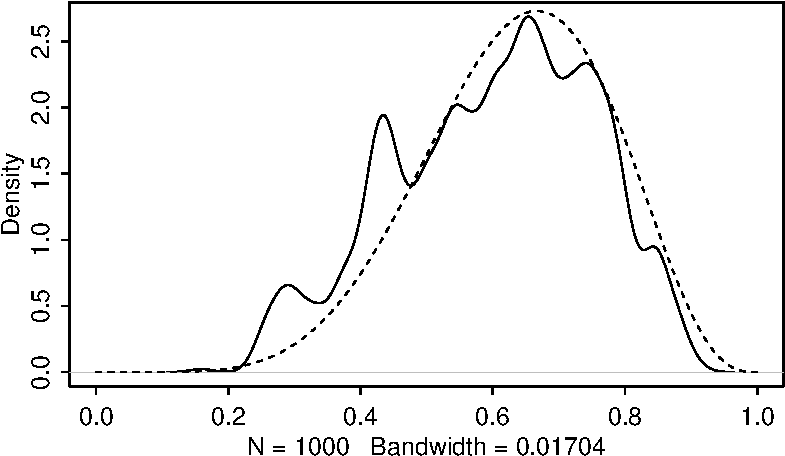
\includegraphics{02-small-and-large-worlds_files/figure-pdf/fig-demo-MCMC-rethinking-1.pdf}

}

\caption{\label{fig-demo-MCMC-rethinking}Demo of the Markov Chain Monte
Carlo (MCMC) method using the globe-tossing data and calculated and
diplayed with the \{\textbf{rethinking}\} package.}

\end{figure}

It's weird. But it works. The above \textbf{METROPOLIS ALGORITHM} is
explained in Chapter 9.

\hypertarget{tidyverse-8}{%
\subsubsection{Tidyverse}\label{tidyverse-8}}

The \{\textbf{brms}\} package uses a version of MCMC to fit Bayesian
models. brms stands for Bayesian Regression Models using `Stan'.

Since one of the main goals of {[}the Kurz version of SR2{]} is to
highlight \{\textbf{brms}\}, we may as well fit a model. This seems like
an appropriately named subsection to do so. First we'll have to load the
package. (If you haven't already installed \{\textbf{brms}\}, you can
find instructions on how to do on
\href{https://github.com/paul-buerkner/brms\#how-do-i-install-brms}{GitHub}
or on the \href{https://paul-buerkner.github.io/brms/}{corresponding
website}.)As an exercise we will re-fit the model with \(W = 24\) and
\(n = 36\) of Listing~\ref{lst-quap-different-sample-size} and
Listing~\ref{lst-fig-quadratic-approx}.

But before we use \{\textbf{brms}\} we need to detach the
\{\textbf{rethinking}\} package.

\begin{quote}
\textbf{R} will not allow us to use a function from one package that
shares the same name as a different function from another package if
both packages are open at the same time. The \textbf{rethinking} and
\textbf{brms} packages are designed for similar purposes and,
unsurprisingly, overlap in some of their function names. To prevent
problems, we will always make sure \textbf{rethinking} is detached
before using \textbf{brms}. To learn more on the topic, see
\href{https://www.r-bloggers.com/2015/04/r-and-package-masking-a-real-life-example/}{this
R-bloggers post}. (This remark comes from
\href{https://bookdown.org/content/4857/geocentric-models.html\#the-data}{section
4.3.1 of the Kurz version}).
\end{quote}

This is the reason why I have not loading the rethinking packages in
code chunks of this file. Instead I referred to every function of the
\{\textbf{rethinking}\} packages directly adding \texttt{rethinking::}
before the function call. This has also the advantage to learn which
functions come from \{\textbf{rethinking}\}.

\begin{tcolorbox}[enhanced jigsaw, colframe=quarto-callout-warning-color-frame, colback=white, toprule=.15mm, breakable, arc=.35mm, bottomtitle=1mm, colbacktitle=quarto-callout-warning-color!10!white, toptitle=1mm, titlerule=0mm, title=\textcolor{quarto-callout-warning-color}{\faExclamationTriangle}\hspace{0.5em}{First compiling}, leftrule=.75mm, opacityback=0, rightrule=.15mm, opacitybacktitle=0.6, bottomrule=.15mm, left=2mm, coltitle=black]

Be patient when you render the following chunk the first time. It need
some time. Furthermore it results in a very long processing message
under the compiled chunk. Again this happens only the first because the
result is stored in the ``fits'' folder which you have to create before
running the chunk.

\end{tcolorbox}

\begin{codelisting}

\caption{Demonstration of the \texttt{brm()} function of the
\{\textbf{brms}\} package.}

\hypertarget{lst-demo-brms}{%
\label{lst-demo-brms}}%
\begin{Shaded}
\begin{Highlighting}[]
\InformationTok{\textasciigrave{}\textasciigrave{}\textasciigrave{}\{r\}}
\CommentTok{\#| label: demo{-}brms}
\CommentTok{\#| attr{-}source: \textquotesingle{}\#lst{-}demo{-}brms lst{-}cap="Demonstration of the \textasciigrave{}brm()\textasciigrave{} function of the \{**brms**\} package."\textquotesingle{}}

\NormalTok{b2}\FloatTok{.1} \OtherTok{\textless{}{-}}
\NormalTok{  brms}\SpecialCharTok{::}\FunctionTok{brm}\NormalTok{(}\AttributeTok{data =} \FunctionTok{list}\NormalTok{(}\AttributeTok{w =} \DecValTok{24}\NormalTok{), }
      \AttributeTok{family =} \FunctionTok{binomial}\NormalTok{(}\AttributeTok{link =} \StringTok{"identity"}\NormalTok{),}
\NormalTok{      w }\SpecialCharTok{|} \FunctionTok{trials}\NormalTok{(}\DecValTok{36}\NormalTok{) }\SpecialCharTok{\textasciitilde{}} \DecValTok{0} \SpecialCharTok{+}\NormalTok{ Intercept,}
\NormalTok{      brms}\SpecialCharTok{::}\FunctionTok{prior}\NormalTok{(}\FunctionTok{beta}\NormalTok{(}\DecValTok{1}\NormalTok{, }\DecValTok{1}\NormalTok{), }\AttributeTok{class =}\NormalTok{ b, }\AttributeTok{lb =} \DecValTok{0}\NormalTok{, }\AttributeTok{ub =} \DecValTok{1}\NormalTok{),}
      \AttributeTok{seed =} \DecValTok{2}\NormalTok{,}
      \AttributeTok{file =} \StringTok{"fits/b02.01"}\NormalTok{)}
\InformationTok{\textasciigrave{}\textasciigrave{}\textasciigrave{}}
\end{Highlighting}
\end{Shaded}

\end{codelisting}

\begin{codelisting}

\caption{Print the result of the demo of the \{\textbf{brms}\} package.}

\hypertarget{lst-print-demo-brms}{%
\label{lst-print-demo-brms}}%
\begin{Shaded}
\begin{Highlighting}[]
\InformationTok{\textasciigrave{}\textasciigrave{}\textasciigrave{}\{r\}}
\CommentTok{\#| label: print{-}result{-}b2.1}
\CommentTok{\#| attr{-}source: \textquotesingle{}\#lst{-}print{-}demo{-}brms lst{-}cap="Print the result of the demo of the \{**brms**\} package."\textquotesingle{}}

\FunctionTok{print}\NormalTok{(b2}\FloatTok{.1}\NormalTok{)}
\InformationTok{\textasciigrave{}\textasciigrave{}\textasciigrave{}}
\end{Highlighting}
\end{Shaded}

\end{codelisting}

\begin{verbatim}
#>  Family: binomial 
#>   Links: mu = identity 
#> Formula: w | trials(36) ~ 0 + Intercept 
#>    Data: list(w = 24) (Number of observations: 1) 
#>   Draws: 4 chains, each with iter = 2000; warmup = 1000; thin = 1;
#>          total post-warmup draws = 4000
#> 
#> Population-Level Effects: 
#>           Estimate Est.Error l-95% CI u-95% CI Rhat Bulk_ESS Tail_ESS
#> Intercept     0.66      0.08     0.50     0.80 1.00     1537     1456
#> 
#> Draws were sampled using sampling(NUTS). For each parameter, Bulk_ESS
#> and Tail_ESS are effective sample size measures, and Rhat is the potential
#> scale reduction factor on split chains (at convergence, Rhat = 1).
\end{verbatim}

A detailed explanation is postponed to chapter 4. Here I will just copy
the notes by Kurz to get a first understand and a starting point for a
later further exploration.

\begin{quote}
For now, focus on the `Intercept' line. As we'll also learn in Chapter
4, the intercept of a typical regression model with no predictors is the
same as its mean. In the special case of a model using the binomial
likelihood, the mean is the probability of a 1 in a given trial,
\(\theta\).

Also, with \{\textbf{brms}\}, there are many ways to summarize the
results of a model. The \texttt{brms::posterior\_summary()} function is
an analogue to \texttt{rethinking::precis()}. We will, however, need to
use \texttt{round()} to reduce the output to a reasonable number of
decimal places.
\end{quote}

\begin{Shaded}
\begin{Highlighting}[]
\InformationTok{\textasciigrave{}\textasciigrave{}\textasciigrave{}\{r\}}
\CommentTok{\#| label: print{-}brms{-}summary}

\NormalTok{brms}\SpecialCharTok{::}\FunctionTok{posterior\_summary}\NormalTok{(b2}\FloatTok{.1}\NormalTok{) }\SpecialCharTok{\%\textgreater{}\%} 
  \FunctionTok{round}\NormalTok{(}\AttributeTok{digits =} \DecValTok{2}\NormalTok{)}
\InformationTok{\textasciigrave{}\textasciigrave{}\textasciigrave{}}
\end{Highlighting}
\end{Shaded}

\begin{verbatim}
#>             Estimate Est.Error  Q2.5 Q97.5
#> b_Intercept     0.66      0.08  0.50  0.80
#> lprior          0.00      0.00  0.00  0.00
#> lp__           -3.98      0.75 -6.03 -3.46
\end{verbatim}

\begin{quote}
The \texttt{b\_Intercept} row is the probability. Don\textquotesingle t
worry about the second line, for now. We\textquotesingle ll cover the
details of \{\textbf{brms\}} model fitting in later chapters. To finish
up, why not plot the results of our model and compare them with those
from \texttt{rethinking::quap()}, above? (See
Picture~\ref{fig-demo-MCMC-rethinking})
\end{quote}

\begin{Shaded}
\begin{Highlighting}[]
\InformationTok{\textasciigrave{}\textasciigrave{}\textasciigrave{}\{r\}}
\CommentTok{\#| label: fig{-}demo{-}MCMC{-}brms}
\CommentTok{\#| fig{-}cap: "Demo of the Markov Chain Monte Carlo (MCMC) method using the globe{-}tossing data with the \{**brms**\} package."}

\NormalTok{brms}\SpecialCharTok{::}\FunctionTok{as\_draws\_df}\NormalTok{(b2}\FloatTok{.1}\NormalTok{) }\SpecialCharTok{\%\textgreater{}\%} 
  \FunctionTok{mutate}\NormalTok{(}\AttributeTok{n =} \StringTok{"n = 36"}\NormalTok{) }\SpecialCharTok{\%\textgreater{}\%}
  
  \FunctionTok{ggplot}\NormalTok{(}\FunctionTok{aes}\NormalTok{(}\AttributeTok{x =}\NormalTok{ b\_Intercept)) }\SpecialCharTok{+}
  \FunctionTok{geom\_density}\NormalTok{(}\AttributeTok{fill =} \StringTok{"black"}\NormalTok{) }\SpecialCharTok{+}
  \FunctionTok{scale\_x\_continuous}\NormalTok{(}\StringTok{"proportion water"}\NormalTok{, }\AttributeTok{limits =} \FunctionTok{c}\NormalTok{(}\DecValTok{0}\NormalTok{, }\DecValTok{1}\NormalTok{)) }\SpecialCharTok{+}
  \FunctionTok{theme}\NormalTok{(}\AttributeTok{panel.grid =} \FunctionTok{element\_blank}\NormalTok{()) }\SpecialCharTok{+}
  \FunctionTok{facet\_wrap}\NormalTok{(}\SpecialCharTok{\textasciitilde{}}\NormalTok{ n)}
\InformationTok{\textasciigrave{}\textasciigrave{}\textasciigrave{}}
\end{Highlighting}
\end{Shaded}

\begin{figure}[H]

{\centering 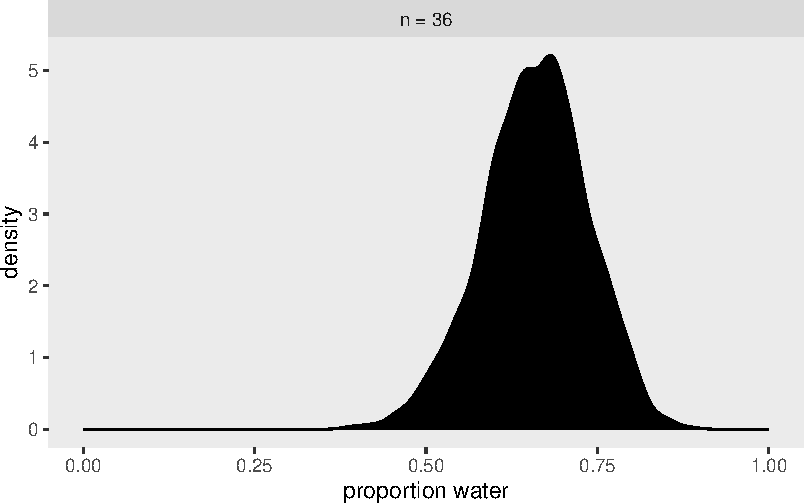
\includegraphics{02-small-and-large-worlds_files/figure-pdf/fig-demo-MCMC-brms-1.pdf}

}

\caption{\label{fig-demo-MCMC-brms}Demo of the Markov Chain Monte Carlo
(MCMC) method using the globe-tossing data with the \{\textbf{brms}\}
package.}

\end{figure}

\begin{quote}
If you\textquotesingle re still confused, cool. This is just a preview.
We\textquotesingle ll start walking through fitting models with
\textbf{brms} in
\href{https://bookdown.org/content/4857/geocentric-models.html\#geocentric-models}{Chapter
4} and we\textquotesingle ll learn a lot about regression with the
binomial likelihood in
\href{https://bookdown.org/content/4857/god-spiked-the-integers.html\#god-spiked-the-integers}{Chapter
11}.
\end{quote}

\hypertarget{reconsideration-1}{%
\subsubsection{Reconsideration}\label{reconsideration-1}}

\hypertarget{bayesian-inference-some-lessons-to-draw}{%
\paragraph{Bayesian Inference: Some Lessons to
Draw}\label{bayesian-inference-some-lessons-to-draw}}

The following list summarizes differences between Bayesian and
Non-Bayesian inference (``Frequentism''):

\begin{enumerate}
\def\labelenumi{\arabic{enumi}.}
\tightlist
\item
  \textbf{No minimum sampling size}: The minimum sampling size in
  Bayesian inference is one. You are going to update each data point at
  its time. For instance you got an estimate every time when you toss
  the globe and the estimate is updated. --- Well, the sample size of
  one is not very informative but that is the power of Bayesian
  inference in not getting over confident. It is always accurately
  representing the relative confidence of plausability we should assign
  to each of the possible proportions.
\item
  \textbf{Shape embodies sample size}: *The shape of the posterior
  distribution embodies all the information that the sample has about
  the process of the proportions. Therefore you do not need to go back
  to the original dataset for new observations. Just take the posterior
  distribution and update it by multiplying the number of ways the new
  data could produce.
\item
  \textbf{No point estimates}: The estimate is the whole distribution.
  It may be fine for communication purposes to talk about some summary
  points of the distribution like the mode and mean. But neither of
  these points is special as a point of estimate. When we do
  calculations we draw predictions from the whole distribution, never
  just from a point of it.
\item
  \textbf{No one true interval}: Intervals are not important in Bayesian
  inference. They are merely summaries of the shape of the distribution.
  There is nothing special in any of these intervals because the
  endpoints of the intervals are not special. Nothing happens of the
  endpoints of the intervals because the interval is arbitrary. (The
  95\% in Non-Bayesian inference is essentially a dogma, a superstition.
  Even in Non-Bayesian statistics it is conceptualized as an arbitrary
  interval.)
\end{enumerate}

\hypertarget{practice}{%
\section{Practice}\label{practice}}

\bookmarksetup{startatroot}

\hypertarget{sec-sampling-the-imaginary}{%
\chapter{Sampling the Imaginary}\label{sec-sampling-the-imaginary}}

\begin{Shaded}
\begin{Highlighting}[]
\InformationTok{\textasciigrave{}\textasciigrave{}\textasciigrave{}\{r\}}
\CommentTok{\#| label: setup}

\FunctionTok{library}\NormalTok{(tidyverse)}
\InformationTok{\textasciigrave{}\textasciigrave{}\textasciigrave{}}
\end{Highlighting}
\end{Shaded}

\begin{verbatim}
#> -- Attaching core tidyverse packages ------------------------ tidyverse 2.0.0 --
#> v dplyr     1.1.2     v readr     2.1.4
#> v forcats   1.0.0     v stringr   1.5.0
#> v ggplot2   3.4.2     v tibble    3.2.1
#> v lubridate 1.9.2     v tidyr     1.3.0
#> v purrr     1.0.1     
#> -- Conflicts ------------------------------------------ tidyverse_conflicts() --
#> x dplyr::filter() masks stats::filter()
#> x dplyr::lag()    masks stats::lag()
#> i Use the conflicted package (<http://conflicted.r-lib.org/>) to force all conflicts to become errors
\end{verbatim}

\hypertarget{vampire-example}{%
\section*{Vampire Example}\label{vampire-example}}
\addcontentsline{toc}{section}{Vampire Example}

\markright{Vampire Example}

\hypertarget{original-9}{%
\subsection*{Original}\label{original-9}}
\addcontentsline{toc}{subsection}{Original}

\hypertarget{a-medical-test-scenario-with-bayes-theorem}{%
\subsubsection*{a) Medical Test Scenario with Bayes
theorem}\label{a-medical-test-scenario-with-bayes-theorem}}
\addcontentsline{toc}{subsubsection}{a) Medical Test Scenario with Bayes
theorem}

\begin{enumerate}
\def\labelenumi{\arabic{enumi}.}
\tightlist
\item
  Suppose there is a blood test that correctly detects vampirism 95\% of
  the time.\(Pr(positivetest|vampire) = 0.95\).
\item
  It's a very accurate test, nearly always catching real vampires. It
  also make mistakes, though, in the form of false positives. One
  percent of the time, it incorrectly diagnoses normal people as
  vampires, \(Pr(positive test result| mortal) = 0.01\).
\item
  The final bit of information we are told is that vampires are rather
  rare, being only 0.1\% of the population, implying
  \(Pr(vampire) = 0.001\).
\end{enumerate}

Suppose now that someone tests positive for vampirism. What's the
probability that he or she is a bloodsucking immortal?

The correct approach is just to use Bayes' theorem to invert the
probability, to compute \(Pr(vampire | positive)\).

\[
\Pr(\text{vampire}|\text{positive}) = \frac{\Pr(\text{positive}|\text{vampire})\Pr(\text{vampire})}{\Pr(\text{positive})}.
\]

where \(Pr(positive)\) is the average probability of a positive test
result, that is,

\[
Pr(positive) = Pr(positive|vampire)Pr(vampire) + Pr(positive|mortal)Pr(1-vampire)
\]

\begin{codelisting}

\caption{Calculated with the Bayes formula}

\hypertarget{lst-bayes-scenario}{%
\label{lst-bayes-scenario}}%
\begin{Shaded}
\begin{Highlighting}[]
\InformationTok{\textasciigrave{}\textasciigrave{}\textasciigrave{}\{r\}}
\CommentTok{\#| label: scenario{-}bayes{-}theorem{-}a}
\CommentTok{\#| attr{-}source: \textquotesingle{}\#lst{-}bayes{-}scenario lst{-}cap="Calculated with the Bayes formula"\textquotesingle{}}

\DocumentationTok{\#\# R code 3.1}
\NormalTok{Pr\_Positive\_Vampire\_a }\OtherTok{\textless{}{-}} \FloatTok{0.95}
\NormalTok{Pr\_Positive\_Mortal\_a }\OtherTok{\textless{}{-}} \FloatTok{0.01}
\NormalTok{Pr\_Vampire\_a }\OtherTok{\textless{}{-}} \FloatTok{0.001}
\NormalTok{Pr\_Positive\_a }\OtherTok{\textless{}{-}}\NormalTok{ Pr\_Positive\_Vampire\_a }\SpecialCharTok{*}\NormalTok{ Pr\_Vampire\_a }\SpecialCharTok{+}
\NormalTok{  Pr\_Positive\_Mortal\_a }\SpecialCharTok{*}\NormalTok{ (}\DecValTok{1} \SpecialCharTok{{-}}\NormalTok{ Pr\_Vampire\_a)}
\NormalTok{(Pr\_Vampire\_Positive\_a }\OtherTok{\textless{}{-}}\NormalTok{ Pr\_Positive\_Vampire\_a }\SpecialCharTok{*}\NormalTok{ Pr\_Vampire\_a }\SpecialCharTok{/}\NormalTok{ Pr\_Positive\_a)}
\InformationTok{\textasciigrave{}\textasciigrave{}\textasciigrave{}}
\end{Highlighting}
\end{Shaded}

\end{codelisting}

\begin{verbatim}
#> [1] 0.08683729
\end{verbatim}

There is only an 8.7\% chance that the suspect is actually a vampire.

\begin{quote}
Most people find this result counterintuitive. And it's a very important
result, because it mimics the structure of many realistic testing
contexts, such as HIV and DNA testing, criminal profiling, and even
statistical significance testing \ldots{} . Whenever the condition of
interest is very rare, having a test that finds all the true cases is
still no guarantee that a positive result carries much information at
all. The reason is that most positive results are false positives, even
when all the true positives are detected correctly.
\end{quote}

\hypertarget{b-medical-test-scenario-with-natural-frequencies}{%
\subsubsection*{b) Medical test scenario with natural
frequencies}\label{b-medical-test-scenario-with-natural-frequencies}}
\addcontentsline{toc}{subsubsection}{b) Medical test scenario with
natural frequencies}

\begin{verbatim}
(1)  In a population of 100,000 people, 100 of them are vampires.
(2)  Of the 100 who are vampires, 95 of them will test positive for vampirism.
(3)  Of the 99,900 mortals, 999 of them will test positive for vampirism.
\end{verbatim}

There are 999 + 95 = 1094 people tested positive. But from these people
only 95 / (999 + 95) = 8.6837294 \% are actually vampires.

Or with a slightly different wording it is still easier to understand:
1. We can just count up the number of people who test positive:
\(95 + 999 = 1094\). 2. Out of these \(1094\) positive tests, \(95\) of
them are real vampires, so that implies:

\[
PR(positive|vampire) = \frac{95}{1094}
\]

\begin{codelisting}

\caption{Calculated with natural figures instead propabilities}

\hypertarget{lst-common-sense-scenario}{%
\label{lst-common-sense-scenario}}%
\begin{Shaded}
\begin{Highlighting}[]
\InformationTok{\textasciigrave{}\textasciigrave{}\textasciigrave{}\{r\}}
\CommentTok{\#| label: scenario{-}common{-}sense{-}a}
\CommentTok{\#| attr{-}source: \textquotesingle{}\#lst{-}common{-}sense{-}scenario lst{-}cap="Calculated with natural figures instead propabilities"\textquotesingle{}}

\DecValTok{95}\SpecialCharTok{/}\DecValTok{1094}
\InformationTok{\textasciigrave{}\textasciigrave{}\textasciigrave{}}
\end{Highlighting}
\end{Shaded}

\end{codelisting}

\begin{verbatim}
#> [1] 0.08683729
\end{verbatim}

The second presentation of the problem, using counts rather than
probabilities, is often called the \emph{frequency format} or
\emph{natural frequencies}. It is easier for people to understand
because are confronted with count in everyday life. Nobody has ever seen
a probability.

\begin{tcolorbox}[enhanced jigsaw, colframe=quarto-callout-note-color-frame, colback=white, toprule=.15mm, breakable, arc=.35mm, bottomtitle=1mm, colbacktitle=quarto-callout-note-color!10!white, toptitle=1mm, titlerule=0mm, title=\textcolor{quarto-callout-note-color}{\faInfo}\hspace{0.5em}{Meta remark: Study guide}, leftrule=.75mm, opacityback=0, rightrule=.15mm, opacitybacktitle=0.6, bottomrule=.15mm, left=2mm, coltitle=black]

This chapter teaches the basic skills for working with samples from the
posterior distribution. We'll begin to use samples to summarize and
simulate model output. The skills learned here will apply to every
problem in the remainder of the book, even though the details of the
models and how the samples are produced will vary.

The chapter exploits the fact that people are better in counts than in
probabilities. We will take the probability distributions from the
previous chapter and sampling from them to produce counts.

\end{tcolorbox}

\begin{quote}
The posterior distribution is a probability distribution. And like all
probability distributions, we can imagine drawing \emph{samples} from
it. The sampled events in this case are parameter values. Most
parameters have no exact empirical realization. The Bayesian formalism
treats parameter distributions as relative plausibility, not as any
physical random process. In any event, randomness is always a property
of information, never of the real world. But inside the computer,
parameters are just as empirical as the outcome of a coin flip or a die
toss or an agricultural experiment. The posterior defines the expected
frequency that different parameter values will appear, once we start
plucking parameters out of it.
\end{quote}

There are two reasons more to use samples:

\begin{enumerate}
\def\labelenumi{\arabic{enumi}.}
\tightlist
\item
  First, many scientists are uncomfortable with integral calculus, even
  though they have strong and valid intuitions about how to summarize
  data. Working with samples transforms a problem in calculus into a
  problem in data summary, into a frequency format problem. An integral
  in a typical Bayesian context is just the total probability in some
  interval.
\item
  Second, some of the most capable methods of computing the posterior
  produce nothing but samples. Many of these methods are variants of
  Markov chain Monte Carlo techniques (MCMC).
\end{enumerate}

Drawing samples from the very simple posterior distribution of the
globe-tossing model might seem as overkill but using this technique from
the start has educational impact: When you inevitably must fit a model
to data using MCMC, you will already know how to make sense of the
output.

\hypertarget{tidyverse-9}{%
\subsection*{Tidyverse}\label{tidyverse-9}}
\addcontentsline{toc}{subsection}{Tidyverse}

\hypertarget{a-medical-test-scenario-with-bayes-theorem-1}{%
\subsubsection*{a) Medical Test Scenario with Bayes
theorem}\label{a-medical-test-scenario-with-bayes-theorem-1}}
\addcontentsline{toc}{subsubsection}{a) Medical Test Scenario with Bayes
theorem}

If you would like to know the probability someone is a vampire given
they test positive to the blood-based vampire test, you compute

\[
Pr(vampire|positive) = \frac{Pr(positive|vampire) \times Pr(vampire)} {Pr(positive)}
\] This is Bayes theorem.

\begin{Shaded}
\begin{Highlighting}[]
\InformationTok{\textasciigrave{}\textasciigrave{}\textasciigrave{}\{r\}}
\CommentTok{\#| label: scenario{-}bayes{-}theorem{-}b}

\FunctionTok{tibble}\NormalTok{(}\AttributeTok{pr\_positive\_vampire\_b =}\NormalTok{ .}\DecValTok{95}\NormalTok{,}
       \AttributeTok{pr\_positive\_mortal\_b  =}\NormalTok{ .}\DecValTok{01}\NormalTok{,}
       \AttributeTok{pr\_vampire\_b          =}\NormalTok{ .}\DecValTok{001}\NormalTok{) }\SpecialCharTok{\%\textgreater{}\%} 
  \FunctionTok{mutate}\NormalTok{(}\AttributeTok{pr\_positive\_b =}\NormalTok{ pr\_positive\_vampire\_b }\SpecialCharTok{*}\NormalTok{ pr\_vampire\_b }\SpecialCharTok{+}\NormalTok{ pr\_positive\_mortal\_b }\SpecialCharTok{*}\NormalTok{ (}\DecValTok{1} \SpecialCharTok{{-}}\NormalTok{ pr\_vampire\_b)) }\SpecialCharTok{\%\textgreater{}\%} 
  \FunctionTok{mutate}\NormalTok{(}\AttributeTok{pr\_vampire\_positive\_b =}\NormalTok{ pr\_positive\_vampire\_b }\SpecialCharTok{*}\NormalTok{ pr\_vampire\_b }\SpecialCharTok{/}\NormalTok{ pr\_positive\_b) }\SpecialCharTok{\%\textgreater{}\%} 
  \FunctionTok{glimpse}\NormalTok{()}
\InformationTok{\textasciigrave{}\textasciigrave{}\textasciigrave{}}
\end{Highlighting}
\end{Shaded}

\begin{verbatim}
#> Rows: 1
#> Columns: 5
#> $ pr_positive_vampire_b <dbl> 0.95
#> $ pr_positive_mortal_b  <dbl> 0.01
#> $ pr_vampire_b          <dbl> 0.001
#> $ pr_positive_b         <dbl> 0.01094
#> $ pr_vampire_positive_b <dbl> 0.08683729
\end{verbatim}

\hypertarget{b-medical-test-scenario-with-natural-frequencies-1}{%
\subsubsection*{b) Medical test scenario with natural
frequencies}\label{b-medical-test-scenario-with-natural-frequencies-1}}
\addcontentsline{toc}{subsubsection}{b) Medical test scenario with
natural frequencies}

\begin{Shaded}
\begin{Highlighting}[]
\InformationTok{\textasciigrave{}\textasciigrave{}\textasciigrave{}\{r\}}
\CommentTok{\#| label: scenario{-}natural{-}frequencies}

\FunctionTok{tibble}\NormalTok{(}\AttributeTok{pr\_vampire\_b2          =} \DecValTok{100} \SpecialCharTok{/} \DecValTok{100000}\NormalTok{,}
       \AttributeTok{pr\_positive\_vampire\_b2 =} \DecValTok{95} \SpecialCharTok{/} \DecValTok{100}\NormalTok{,}
       \AttributeTok{pr\_positive\_mortal\_b2  =} \DecValTok{999} \SpecialCharTok{/} \DecValTok{99900}\NormalTok{) }\SpecialCharTok{\%\textgreater{}\%} 
  \FunctionTok{mutate}\NormalTok{(}\AttributeTok{pr\_positive\_b2 =} \DecValTok{95} \SpecialCharTok{+} \DecValTok{999}\NormalTok{) }\SpecialCharTok{\%\textgreater{}\%} 
  \FunctionTok{mutate}\NormalTok{(}\AttributeTok{pr\_vampire\_positive\_b2 =}\NormalTok{ pr\_positive\_vampire\_b2 }\SpecialCharTok{*} \DecValTok{100} \SpecialCharTok{/}\NormalTok{ pr\_positive\_b2) }\SpecialCharTok{\%\textgreater{}\%} 
  \FunctionTok{glimpse}\NormalTok{()}
\InformationTok{\textasciigrave{}\textasciigrave{}\textasciigrave{}}
\end{Highlighting}
\end{Shaded}

\begin{verbatim}
#> Rows: 1
#> Columns: 5
#> $ pr_vampire_b2          <dbl> 0.001
#> $ pr_positive_vampire_b2 <dbl> 0.95
#> $ pr_positive_mortal_b2  <dbl> 0.01
#> $ pr_positive_b2         <dbl> 1094
#> $ pr_vampire_positive_b2 <dbl> 0.08683729
\end{verbatim}

\hypertarget{sampling-from-a-grid-approximate-posterior}{%
\section{Sampling from a grid-approximate
posterior}\label{sampling-from-a-grid-approximate-posterior}}

\hypertarget{original-10}{%
\subsection{Original}\label{original-10}}

\hypertarget{grid-approximation-1}{%
\subsubsection{Grid approximation}\label{grid-approximation-1}}

Before we are going to draw samples from the posterior distribution we
need to compute the distribution. Again we are using grid approximation.

\begin{codelisting}

\caption{Generate the posterior distribution form the globe-tossing
example}

\hypertarget{lst-grid-approx-a}{%
\label{lst-grid-approx-a}}%
\begin{Shaded}
\begin{Highlighting}[]
\InformationTok{\textasciigrave{}\textasciigrave{}\textasciigrave{}\{r\}}
\CommentTok{\#| label: grid{-}approx{-}a}
\CommentTok{\#| attr{-}source: \textquotesingle{}\#lst{-}grid{-}approx{-}a lst{-}cap="Generate the posterior distribution form the globe{-}tossing example"\textquotesingle{}}

\DocumentationTok{\#\#\# R code 3.2 \#\#\#\#\#\#\#\#\#\#\#\#\#\#\#\#\#\#\#\#\#\#\#\#\#\#}
\CommentTok{\# change prob\_b to prior}
\CommentTok{\# change prob\_data to likelihood}
\CommentTok{\# added variables: n, n\_success, n\_trials}

\NormalTok{n\_grid\_a }\OtherTok{\textless{}{-}}\NormalTok{ 1000L}
\NormalTok{n\_success\_a }\OtherTok{\textless{}{-}}\NormalTok{ 6L}
\NormalTok{n\_trials\_a }\OtherTok{\textless{}{-}}\NormalTok{  9L}


\NormalTok{p\_grid\_a }\OtherTok{\textless{}{-}} \FunctionTok{seq}\NormalTok{(}\AttributeTok{from =} \DecValTok{0}\NormalTok{, }\AttributeTok{to =} \DecValTok{1}\NormalTok{, }\AttributeTok{length.out =}\NormalTok{ n\_grid\_a)}
\NormalTok{prior\_a }\OtherTok{\textless{}{-}} \FunctionTok{rep}\NormalTok{(}\DecValTok{1}\NormalTok{, n\_grid\_a) }\CommentTok{\# = prior, assumed as uniform distribution}
\NormalTok{likelihood\_a }\OtherTok{\textless{}{-}} \FunctionTok{dbinom}\NormalTok{(n\_success\_a, }\AttributeTok{size =}\NormalTok{ n\_trials\_a, }\AttributeTok{prob =}\NormalTok{ p\_grid\_a) }\CommentTok{\# = likelihood}
\NormalTok{posterior\_a }\OtherTok{\textless{}{-}}\NormalTok{ likelihood\_a }\SpecialCharTok{*}\NormalTok{ prior\_a}
\NormalTok{posterior\_a }\OtherTok{\textless{}{-}}\NormalTok{ posterior\_a }\SpecialCharTok{/} \FunctionTok{sum}\NormalTok{(posterior\_a)}
\InformationTok{\textasciigrave{}\textasciigrave{}\textasciigrave{}}
\end{Highlighting}
\end{Shaded}

\end{codelisting}

\begin{quote}
Now we wish to draw 10,000 samples from this posterior. Imagine the
posterior is a bucket full of parameter values, numbers such as 0.1,
0.7, 0.5, 1, etc. Within the bucket, each value exists in proportion to
its posterior probability, such that values near the peak are much more
common than those in the tails. We're going to scoop out 10,000 values
from the bucket. Provided the bucket is well mixed, the resulting
samples will have the same proportions as the exact posterior density.
Therefore the individual values of \emph{p} will appear in our samples
in proportion to the posterior plausibility of each value.
\end{quote}

\hypertarget{drawing-samples}{%
\subsubsection{Drawing samples}\label{drawing-samples}}

\begin{codelisting}[H]

\caption{Draw 1000 Samples from the posterior distribution, using
\texttt{base::set.seed(3)}}

\hypertarget{lst-draw-samples-a}{%
\label{lst-draw-samples-a}}%
\begin{Shaded}
\begin{Highlighting}[]
\InformationTok{\textasciigrave{}\textasciigrave{}\textasciigrave{}\{r\}}
\CommentTok{\#| label: draw{-}samples{-}a}
\CommentTok{\#| attr{-}source: \textquotesingle{}\#lst{-}draw{-}samples{-}a lst{-}cap="Draw 1000 Samples from the posterior distribution, using \textasciigrave{}base::set.seed(3)\textasciigrave{}"\textquotesingle{}}

\NormalTok{n\_samples\_a }\OtherTok{\textless{}{-}} \FloatTok{1e4}

\FunctionTok{set.seed}\NormalTok{(}\DecValTok{3}\NormalTok{) }\hspace*{\fill}\NormalTok{\circled{1}}

\DocumentationTok{\#\# R code 3.3 \#\#\#\#\#\#\#\#\#\#\#\#\#\#\#\#\#\#\#\#\#\#\#\#\#\#\#\#\#\#\#\#\#\#\#\#\#\#\#\#\#\#}
\NormalTok{samples\_a }\OtherTok{\textless{}{-}} \FunctionTok{sample}\NormalTok{(p\_grid\_a, }\AttributeTok{prob =}\NormalTok{ posterior\_a, }
                    \AttributeTok{size =}\NormalTok{ n\_samples\_a, }\AttributeTok{replace =} \ConstantTok{TRUE}\NormalTok{) }\hspace*{\fill}\NormalTok{\circled{2}}
\InformationTok{\textasciigrave{}\textasciigrave{}\textasciigrave{}}
\end{Highlighting}
\end{Shaded}

\end{codelisting}

\begin{description}
\tightlist
\item[\circled{1}]
I have included the \texttt{base::set.seed()} command myself to provide
reproducibility. With this code line you will get the same results in
your sampling process because it is not really a random procedure but
the outcome of a complex algorithm that can be configured by the
\texttt{set.seed()} function.
\item[\circled{2}]
The workhorse here is \texttt{base::sample}, which randomly pulls values
from a vector. The vector in this case is \texttt{p\_grid\_a}, the grid
of 1000 (1e3) parameter values. The probability of each value is given
by \texttt{posterior\_a}, which we computed with
Listing~\ref{lst-grid-approx-a}.
\end{description}

To compare the calculated values with variant b (the tidyverse version),
I bound the three vectors with \texttt{base::cbind()} together into a
matrix and displayed the first six lines with \texttt{utils::head()}.
Additionally I also displayed the first 10 values of \texttt{samples\_a}
vector.

\begin{Shaded}
\begin{Highlighting}[]
\InformationTok{\textasciigrave{}\textasciigrave{}\textasciigrave{}\{r\}}
\CommentTok{\#| label: display{-}grid\_result\_a}

\CommentTok{\# display grid results to compare with variant b}
\NormalTok{d\_a }\OtherTok{\textless{}{-}} \FunctionTok{cbind}\NormalTok{(p\_grid\_a, prior\_a, likelihood\_a, posterior\_a) }
\FunctionTok{head}\NormalTok{(d\_a, }\DecValTok{10}\NormalTok{)}
\InformationTok{\textasciigrave{}\textasciigrave{}\textasciigrave{}}
\end{Highlighting}
\end{Shaded}

\begin{verbatim}
#>          p_grid_a prior_a likelihood_a  posterior_a
#>  [1,] 0.000000000       1 0.000000e+00 0.000000e+00
#>  [2,] 0.001001001       1 8.425225e-17 8.433659e-19
#>  [3,] 0.002002002       1 5.375951e-15 5.381333e-17
#>  [4,] 0.003003003       1 6.105137e-14 6.111249e-16
#>  [5,] 0.004004004       1 3.419945e-13 3.423368e-15
#>  [6,] 0.005005005       1 1.300676e-12 1.301978e-14
#>  [7,] 0.006006006       1 3.872087e-12 3.875963e-14
#>  [8,] 0.007007007       1 9.734489e-12 9.744233e-14
#>  [9,] 0.008008008       1 2.162473e-11 2.164638e-13
#> [10,] 0.009009009       1 4.370695e-11 4.375070e-13
\end{verbatim}

Furthermore I also displayed the first 10 values of \texttt{samples\_a}
vector.

\begin{Shaded}
\begin{Highlighting}[]
\InformationTok{\textasciigrave{}\textasciigrave{}\textasciigrave{}\{r\}}
\CommentTok{\#| label: display{-}samples\_result\_a}

\CommentTok{\# display sample results to compare with variant b}
\FunctionTok{head}\NormalTok{(samples\_a, }\DecValTok{10}\NormalTok{)}
\InformationTok{\textasciigrave{}\textasciigrave{}\textasciigrave{}}
\end{Highlighting}
\end{Shaded}

\begin{verbatim}
#>  [1] 0.5645646 0.6516517 0.5475475 0.5905906 0.5955956 0.7877878 0.7267267
#>  [8] 0.4914915 0.7507508 0.4494494
\end{verbatim}

\hypertarget{plot-samples-distribution}{%
\subsubsection{Plot samples
distribution}\label{plot-samples-distribution}}

\begin{Shaded}
\begin{Highlighting}[]
\InformationTok{\textasciigrave{}\textasciigrave{}\textasciigrave{}\{r\}}
\CommentTok{\#| label: fig{-}scatterplot{-}samples{-}a}
\CommentTok{\#| fig{-}cap: "Scatterplot of the drawn samples (Version a)"}

\DocumentationTok{\#\# R code 3.4 \#\#\#\#\#\#\#\#\#}
\FunctionTok{plot}\NormalTok{(samples\_a)}
\InformationTok{\textasciigrave{}\textasciigrave{}\textasciigrave{}}
\end{Highlighting}
\end{Shaded}

\begin{figure}[H]

{\centering 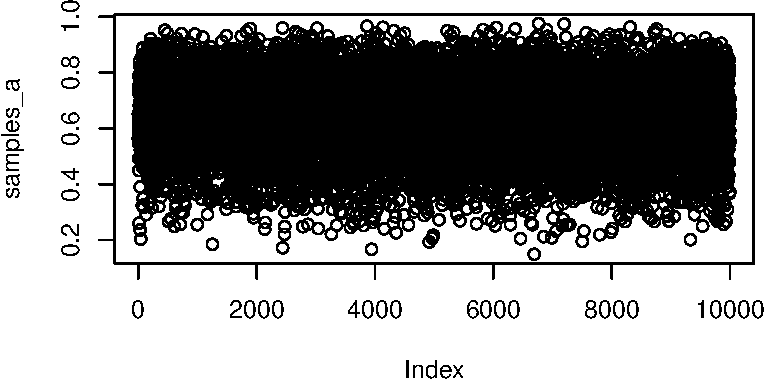
\includegraphics{03-sampling-the-imaginary_files/figure-pdf/fig-scatterplot-samples-a-1.pdf}

}

\caption{\label{fig-scatterplot-samples-a}Scatterplot of the drawn
samples (Version a)}

\end{figure}

In Picture~\ref{fig-scatterplot-samples-a}, it is as if you are flying
over the posterior distribution, looking down on it. There are many more
samples from the dense region near 0.6 and very few samples below 0.25.

\begin{Shaded}
\begin{Highlighting}[]
\InformationTok{\textasciigrave{}\textasciigrave{}\textasciigrave{}\{r\}}
\CommentTok{\#| label: fig{-}density{-}samples{-}a}
\CommentTok{\#| fig{-}cap: "Density estimate of the drawn samples (Version a)"}

\DocumentationTok{\#\# R code 3.5 \#\#\#\#\#\#\#\#\#\#\#\#\#}
\NormalTok{rethinking}\SpecialCharTok{::}\FunctionTok{dens}\NormalTok{(samples\_a)}
\InformationTok{\textasciigrave{}\textasciigrave{}\textasciigrave{}}
\end{Highlighting}
\end{Shaded}

\begin{figure}[H]

{\centering 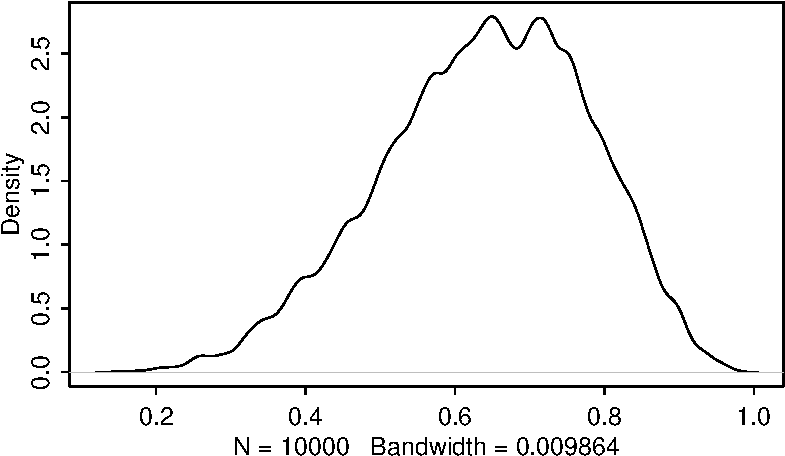
\includegraphics{03-sampling-the-imaginary_files/figure-pdf/fig-density-samples-a-1.pdf}

}

\caption{\label{fig-density-samples-a}Density estimate of the drawn
samples (Version a)}

\end{figure}

Plot Picture~\ref{fig-density-samples-a} shows the density estimate
computed from our sampling process. The estimated density is very
similar to ideal posterior you computed via grid approximation. If you
draw even more samples, maybe 1e5 or 1e6, the density estimate will get
more and more similar to the ideal. This is shown in the tidyverse
version Picture~\ref{fig-density-samples-b2}.

\hypertarget{tidyverse-10}{%
\subsection{Tidyverse}\label{tidyverse-10}}

\hypertarget{grid-approximation-2}{%
\subsubsection{Grid approximation}\label{grid-approximation-2}}

\begin{Shaded}
\begin{Highlighting}[]
\InformationTok{\textasciigrave{}\textasciigrave{}\textasciigrave{}\{r\}}
\CommentTok{\#| label: grid{-}approx{-}b}

\CommentTok{\# how many grid points would you like?}
\NormalTok{n\_grid\_b }\OtherTok{\textless{}{-}}\NormalTok{ 1000L}
\NormalTok{n\_success\_b }\OtherTok{\textless{}{-}}\NormalTok{ 6L}
\NormalTok{n\_trials\_b  }\OtherTok{\textless{}{-}}\NormalTok{ 9L}

\NormalTok{(}
\NormalTok{  d\_b }\OtherTok{\textless{}{-}}
  \FunctionTok{tibble}\NormalTok{(}\AttributeTok{p\_grid\_b =} \FunctionTok{seq}\NormalTok{(}\AttributeTok{from =} \DecValTok{0}\NormalTok{, }\AttributeTok{to =} \DecValTok{1}\NormalTok{, }\AttributeTok{length.out =}\NormalTok{ n\_grid\_b),}
         \CommentTok{\# note we\textquotesingle{}re still using a flat uniform prior}
         \AttributeTok{prior\_b  =} \DecValTok{1}\NormalTok{) }\SpecialCharTok{\%\textgreater{}\%} 
  \FunctionTok{mutate}\NormalTok{(}\AttributeTok{likelihood\_b =} \FunctionTok{dbinom}\NormalTok{(n\_success\_b, }\AttributeTok{size =}\NormalTok{ n\_trials\_b, }\AttributeTok{prob =}\NormalTok{ p\_grid\_b)) }\SpecialCharTok{\%\textgreater{}\%} 
  \FunctionTok{mutate}\NormalTok{(}\AttributeTok{posterior\_b =}\NormalTok{ (likelihood\_b }\SpecialCharTok{*}\NormalTok{ prior\_b) }\SpecialCharTok{/} \FunctionTok{sum}\NormalTok{(likelihood\_b }\SpecialCharTok{*}\NormalTok{ prior\_b))}
\NormalTok{)}
\InformationTok{\textasciigrave{}\textasciigrave{}\textasciigrave{}}
\end{Highlighting}
\end{Shaded}

\begin{verbatim}
#> # A tibble: 1,000 x 4
#>    p_grid_b prior_b likelihood_b posterior_b
#>       <dbl>   <dbl>        <dbl>       <dbl>
#>  1  0             1     0           0       
#>  2  0.00100       1     8.43e-17    8.43e-19
#>  3  0.00200       1     5.38e-15    5.38e-17
#>  4  0.00300       1     6.11e-14    6.11e-16
#>  5  0.00400       1     3.42e-13    3.42e-15
#>  6  0.00501       1     1.30e-12    1.30e-14
#>  7  0.00601       1     3.87e-12    3.88e-14
#>  8  0.00701       1     9.73e-12    9.74e-14
#>  9  0.00801       1     2.16e-11    2.16e-13
#> 10  0.00901       1     4.37e-11    4.38e-13
#> # i 990 more rows
\end{verbatim}

\hypertarget{drawing-samples-1}{%
\subsubsection{Drawing samples}\label{drawing-samples-1}}

\begin{tcolorbox}[enhanced jigsaw, colframe=quarto-callout-caution-color-frame, colback=white, toprule=.15mm, breakable, arc=.35mm, bottomtitle=1mm, colbacktitle=quarto-callout-caution-color!10!white, toptitle=1mm, titlerule=0mm, title=\textcolor{quarto-callout-caution-color}{\faFire}\hspace{0.5em}{Changing variable names}, leftrule=.75mm, opacityback=0, rightrule=.15mm, opacitybacktitle=0.6, bottomrule=.15mm, left=2mm, coltitle=black]

We've renamed McElreath's \texttt{prob\_p} and \texttt{prob\_data} as
\texttt{prior\_b} and \texttt{likelihood\_b}, respectively. Now we'll
use the \texttt{dplyr::slice\_sample()} function to sample rows from
\texttt{d\_b}, saving them as \texttt{samples\_b}.

To get the same variable name of the sample results in version a and b I
will change in the following code chunk \texttt{p\_grid\_b} to
\texttt{samples\_b}. So I can compare the vector \texttt{samples\_a}
with the column \texttt{samples\_b}of the tibble with the same name
(\texttt{samples\_b}).

Additionally: To see the difference between grid and samples I will add
``\_sample'' to all the other variable names. For reasons of consistence
I will also change the name of ``prior\_b''

\end{tcolorbox}

\begin{Shaded}
\begin{Highlighting}[]
\InformationTok{\textasciigrave{}\textasciigrave{}\textasciigrave{}\{r\}}
\CommentTok{\#| label: draw{-}samples{-}b}

\CommentTok{\# how many samples would you like?}
\NormalTok{n\_samples\_b }\OtherTok{\textless{}{-}} \FloatTok{1e4}

\CommentTok{\# make it reproducible}
\FunctionTok{set.seed}\NormalTok{(}\DecValTok{3}\NormalTok{)}

\NormalTok{samples\_b }\OtherTok{\textless{}{-}}
\NormalTok{  d\_b }\SpecialCharTok{\%\textgreater{}\%} 
    \FunctionTok{slice\_sample}\NormalTok{(}\AttributeTok{n =}\NormalTok{ n\_samples\_b, }\AttributeTok{weight\_by =}\NormalTok{ posterior\_b, }\AttributeTok{replace =}\NormalTok{ T)}


\NormalTok{( }
\NormalTok{    samples\_b }\OtherTok{\textless{}{-}}\NormalTok{ samples\_b }\SpecialCharTok{|\textgreater{}}
        \FunctionTok{rename}\NormalTok{(}\AttributeTok{samples\_b =}\NormalTok{ p\_grid\_b,}
               \AttributeTok{likelihood\_samples\_b =}\NormalTok{ likelihood\_b,}
               \AttributeTok{prior\_samples\_prior\_b =}\NormalTok{ prior\_b,}
               \AttributeTok{posterior\_samples\_b =}\NormalTok{ posterior\_b)}
\NormalTok{)}
\InformationTok{\textasciigrave{}\textasciigrave{}\textasciigrave{}}
\end{Highlighting}
\end{Shaded}

\begin{verbatim}
#> # A tibble: 10,000 x 4
#>    samples_b prior_samples_prior_b likelihood_samples_b posterior_samples_b
#>        <dbl>                 <dbl>                <dbl>               <dbl>
#>  1     0.565                     1                0.225             0.00225
#>  2     0.652                     1                0.272             0.00272
#>  3     0.548                     1                0.210             0.00210
#>  4     0.591                     1                0.245             0.00245
#>  5     0.596                     1                0.248             0.00248
#>  6     0.788                     1                0.192             0.00192
#>  7     0.727                     1                0.253             0.00253
#>  8     0.491                     1                0.156             0.00156
#>  9     0.751                     1                0.233             0.00233
#> 10     0.449                     1                0.116             0.00116
#> # i 9,990 more rows
\end{verbatim}

The column \texttt{samples\_b} of the tibble with the same name (watch
out not to confuse these two objects) is identical with the vector
\texttt{samples\_a}. This \texttt{base::identical()} results in
different sampling processes was the work of \texttt{set.seed(3)}.

\begin{Shaded}
\begin{Highlighting}[]
\InformationTok{\textasciigrave{}\textasciigrave{}\textasciigrave{}\{r\}}
\CommentTok{\#| label: test{-}if{-}samples{-}identical}

\FunctionTok{identical}\NormalTok{(samples\_a, samples\_b}\SpecialCharTok{$}\NormalTok{samples\_b)}
\InformationTok{\textasciigrave{}\textasciigrave{}\textasciigrave{}}
\end{Highlighting}
\end{Shaded}

\begin{verbatim}
#> [1] TRUE
\end{verbatim}

With the \texttt{utils::str()} function you will get a result with
shorter figures that is better adapted to a small screen.

\begin{Shaded}
\begin{Highlighting}[]
\InformationTok{\textasciigrave{}\textasciigrave{}\textasciigrave{}\{r\}}
\CommentTok{\#| label: str{-}samples{-}b}

\FunctionTok{str}\NormalTok{(samples\_b)}
\InformationTok{\textasciigrave{}\textasciigrave{}\textasciigrave{}}
\end{Highlighting}
\end{Shaded}

\begin{verbatim}
#> tibble [10,000 x 4] (S3: tbl_df/tbl/data.frame)
#>  $ samples_b            : num [1:10000] 0.565 0.652 0.548 0.591 0.596 ...
#>  $ prior_samples_prior_b: num [1:10000] 1 1 1 1 1 1 1 1 1 1 ...
#>  $ likelihood_samples_b : num [1:10000] 0.225 0.272 0.21 0.245 0.248 ...
#>  $ posterior_samples_b  : num [1:10000] 0.00225 0.00272 0.0021 0.00245 0.00248 ...
\end{verbatim}

An alternative of the tidyverse approach is \texttt{dplyr::glimpse()}.

\begin{Shaded}
\begin{Highlighting}[]
\InformationTok{\textasciigrave{}\textasciigrave{}\textasciigrave{}\{r\}}
\CommentTok{\#| label: glimpse{-}samples{-}b}

\FunctionTok{glimpse}\NormalTok{(samples\_b)}
\InformationTok{\textasciigrave{}\textasciigrave{}\textasciigrave{}}
\end{Highlighting}
\end{Shaded}

\begin{verbatim}
#> Rows: 10,000
#> Columns: 4
#> $ samples_b             <dbl> 0.5645646, 0.6516517, 0.5475475, 0.5905906, 0.59~
#> $ prior_samples_prior_b <dbl> 1, 1, 1, 1, 1, 1, 1, 1, 1, 1, 1, 1, 1, 1, 1, 1, ~
#> $ likelihood_samples_b  <dbl> 0.22455994, 0.27190272, 0.20966655, 0.24460869, ~
#> $ posterior_samples_b   <dbl> 0.0022478473, 0.0027217490, 0.0020987643, 0.0024~
\end{verbatim}

Now we can plot the left panel of Figure 3.1 with
\texttt{ggplot2::geom\_point()}. But before we do, we'll need to add a
variable numbering the samples.

\hypertarget{plot-samples-distribution-1}{%
\subsubsection{Plot samples
distribution}\label{plot-samples-distribution-1}}

\begin{Shaded}
\begin{Highlighting}[]
\InformationTok{\textasciigrave{}\textasciigrave{}\textasciigrave{}\{r\}}
\CommentTok{\#| label: fig{-}scatterplot{-}samples{-}b}
\CommentTok{\#| fig{-}cap: "Scatterplot of the drawn samples (Version b)"}

\NormalTok{samples\_b }\SpecialCharTok{\%\textgreater{}\%} 
  \FunctionTok{mutate}\NormalTok{(}\AttributeTok{sample\_number =} \DecValTok{1}\SpecialCharTok{:}\FunctionTok{n}\NormalTok{()) }\SpecialCharTok{\%\textgreater{}\%} 
  
  \FunctionTok{ggplot}\NormalTok{(}\FunctionTok{aes}\NormalTok{(}\AttributeTok{x =}\NormalTok{ sample\_number, }\AttributeTok{y =}\NormalTok{ samples\_b)) }\SpecialCharTok{+}
  \FunctionTok{geom\_point}\NormalTok{(}\AttributeTok{alpha =} \DecValTok{1}\SpecialCharTok{/}\DecValTok{10}\NormalTok{) }\SpecialCharTok{+}
  \FunctionTok{scale\_y\_continuous}\NormalTok{(}\StringTok{"proportion of water (p)"}\NormalTok{, }\AttributeTok{limits =} \FunctionTok{c}\NormalTok{(}\DecValTok{0}\NormalTok{, }\DecValTok{1}\NormalTok{)) }\SpecialCharTok{+}
  \FunctionTok{xlab}\NormalTok{(}\StringTok{"sample number"}\NormalTok{)}
\InformationTok{\textasciigrave{}\textasciigrave{}\textasciigrave{}}
\end{Highlighting}
\end{Shaded}

\begin{figure}[H]

{\centering 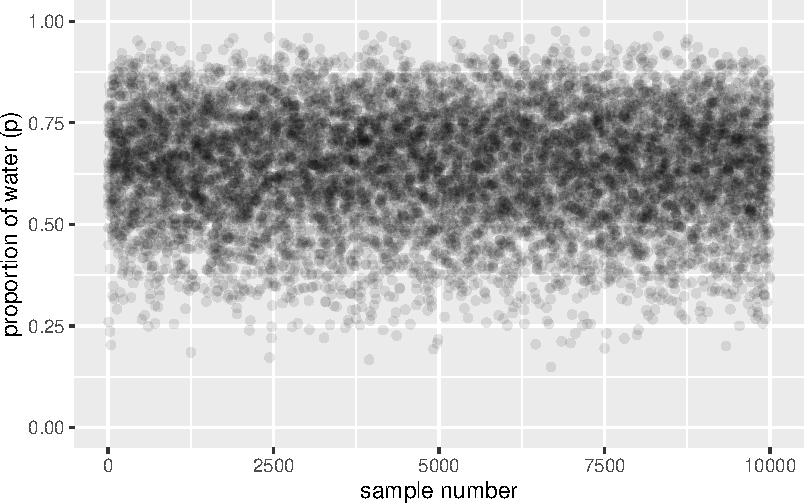
\includegraphics{03-sampling-the-imaginary_files/figure-pdf/fig-scatterplot-samples-b-1.pdf}

}

\caption{\label{fig-scatterplot-samples-b}Scatterplot of the drawn
samples (Version b)}

\end{figure}

We'll make the density in the right panel with
\texttt{ggplot2::geom\_density()}.

\begin{Shaded}
\begin{Highlighting}[]
\InformationTok{\textasciigrave{}\textasciigrave{}\textasciigrave{}\{r\}}
\CommentTok{\#| label: fig{-}density{-}samples{-}b}
\CommentTok{\#| fig{-}cap: "Density estimate of the drawn samples (Version b)"}

\NormalTok{samples\_b }\SpecialCharTok{\%\textgreater{}\%} 
  \FunctionTok{ggplot}\NormalTok{(}\FunctionTok{aes}\NormalTok{(}\AttributeTok{x =}\NormalTok{ samples\_b)) }\SpecialCharTok{+}
  \FunctionTok{geom\_density}\NormalTok{(}\AttributeTok{fill =} \StringTok{"grey"}\NormalTok{) }\SpecialCharTok{+}
  \FunctionTok{scale\_x\_continuous}\NormalTok{(}\StringTok{"proportion of water (p)"}\NormalTok{, }\AttributeTok{limits =} \FunctionTok{c}\NormalTok{(}\DecValTok{0}\NormalTok{, }\DecValTok{1}\NormalTok{))}
\InformationTok{\textasciigrave{}\textasciigrave{}\textasciigrave{}}
\end{Highlighting}
\end{Shaded}

\begin{figure}[H]

{\centering 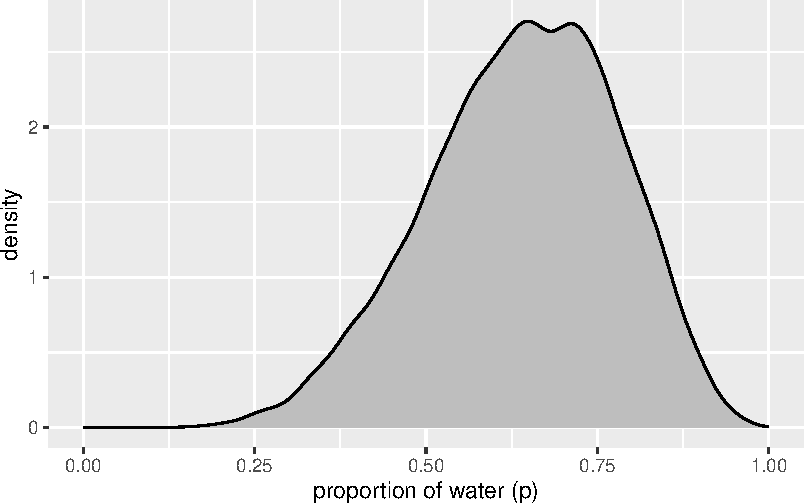
\includegraphics{03-sampling-the-imaginary_files/figure-pdf/fig-density-samples-b-1.pdf}

}

\caption{\label{fig-density-samples-b}Density estimate of the drawn
samples (Version b)}

\end{figure}

Compare this somewhat smoother Picture~\ref{fig-density-samples-b} with
Picture~\ref{fig-density-samples-a}.

If we keep increasing the number of samples we will get a better
approximation to the ideal posterior distribution we have computed via
grid approximation. Here's what it looks like with \texttt{1e6}.

\begin{Shaded}
\begin{Highlighting}[]
\InformationTok{\textasciigrave{}\textasciigrave{}\textasciigrave{}\{r\}}
\CommentTok{\#| label: fig{-}density{-}samples{-}b2}
\CommentTok{\#| fig{-}cap: "Density estimate of 1e6 drawn samples (Version b)"}

\FunctionTok{set.seed}\NormalTok{(}\DecValTok{3}\NormalTok{)}

\NormalTok{d\_b }\SpecialCharTok{\%\textgreater{}\%} 
  \FunctionTok{slice\_sample}\NormalTok{(}\AttributeTok{n =} \FloatTok{1e6}\NormalTok{, }\AttributeTok{weight\_by =}\NormalTok{ posterior\_b, }\AttributeTok{replace =}\NormalTok{ T) }\SpecialCharTok{\%\textgreater{}\%} 
  \FunctionTok{ggplot}\NormalTok{(}\FunctionTok{aes}\NormalTok{(}\AttributeTok{x =}\NormalTok{ p\_grid\_b)) }\SpecialCharTok{+}
  \FunctionTok{geom\_density}\NormalTok{(}\AttributeTok{fill =} \StringTok{"grey"}\NormalTok{) }\SpecialCharTok{+}
  \FunctionTok{scale\_x\_continuous}\NormalTok{(}\StringTok{"proportion of water (p)"}\NormalTok{, }\AttributeTok{limits =} \FunctionTok{c}\NormalTok{(}\DecValTok{0}\NormalTok{, }\DecValTok{1}\NormalTok{))}
\InformationTok{\textasciigrave{}\textasciigrave{}\textasciigrave{}}
\end{Highlighting}
\end{Shaded}

\begin{figure}[H]

{\centering 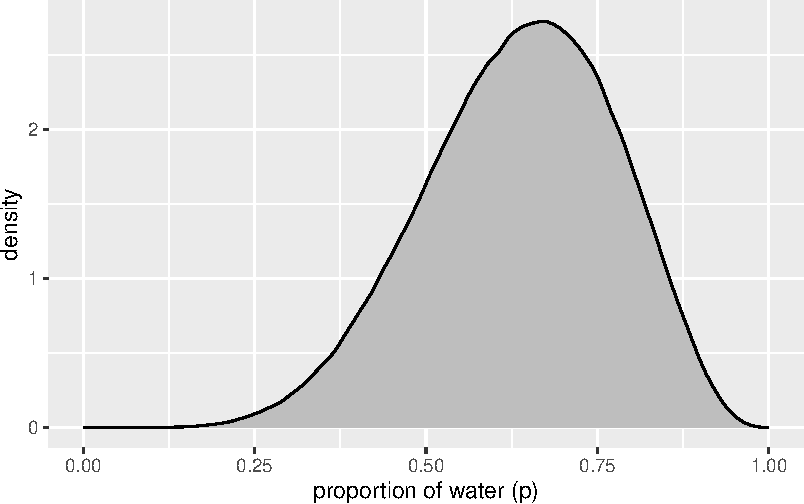
\includegraphics{03-sampling-the-imaginary_files/figure-pdf/fig-density-samples-b2-1.pdf}

}

\caption{\label{fig-density-samples-b2}Density estimate of 1e6 drawn
samples (Version b)}

\end{figure}

\hypertarget{sampling-to-summarize}{%
\section{Sampling to Summarize}\label{sampling-to-summarize}}

\hypertarget{three-questions-asked}{%
\subsection*{Three questions asked}\label{three-questions-asked}}
\addcontentsline{toc}{subsection}{Three questions asked}

All we have done so far is crudely replicate the posterior density we
had already computed in the previous chapter. Now it is time to use
these samples to describe and understand the posterior.

The first step in understanding the posterior distribution is to
summarize it. Exactly how it is summarized depends upon your purpose.
But common questions include:

\begin{itemize}
\tightlist
\item
  How much posterior probability lies below some parameter value?
\item
  How much posterior probability lies between two parameter values?
\item
  Which parameter value marks the lower 5\% of the posterior
  probability?
\item
  Which range of parameter values contains 90\% of the posterior
  probability?
\item
  Which parameter value has highest posterior probability?
\end{itemize}

The above list of questions can be divided into three inquiries:

\begin{enumerate}
\def\labelenumi{\arabic{enumi}.}
\tightlist
\item
  Questions about intervals of defined boundaries.
\item
  Questions about intervals of defined probability mass.
\item
  Questions about point estimates.
\end{enumerate}

\hypertarget{intervals-of-defined-boundaries}{%
\subsection{Intervals of Defined
Boundaries}\label{intervals-of-defined-boundaries}}

\hypertarget{original-11}{%
\subsubsection{Original}\label{original-11}}

\hypertarget{grid-approach}{%
\paragraph{Grid approach}\label{grid-approach}}

For instance: What is the probability that the proportion of water is
less than 0.5?

\begin{Shaded}
\begin{Highlighting}[]
\InformationTok{\textasciigrave{}\textasciigrave{}\textasciigrave{}\{r\}}
\CommentTok{\#| label: grid{-}boundaries{-}a}

\DocumentationTok{\#\# R code 3.6}
\CommentTok{\# add up posterior probability where p \textless{} 0.5}
\FunctionTok{sum}\NormalTok{(posterior\_a[p\_grid\_a }\SpecialCharTok{\textless{}} \FloatTok{0.5}\NormalTok{])}
\InformationTok{\textasciigrave{}\textasciigrave{}\textasciigrave{}}
\end{Highlighting}
\end{Shaded}

\begin{verbatim}
#> [1] 0.1718746
\end{verbatim}

About 17\% of the posterior probability is below 0.5. Couldn't be
easier.

\hypertarget{sampling-approach}{%
\paragraph{Sampling approach}\label{sampling-approach}}

But this easy calculation based on grid approximation is often no
practical when there are more parameters. So let's try the sampling
approach:

To use the samples from the posterior you have to add up all of the
samples below 0.5, but also divide the resulting count by the total
number of samples. In other words, find the frequency of parameter
values below 0.5:

\begin{Shaded}
\begin{Highlighting}[]
\InformationTok{\textasciigrave{}\textasciigrave{}\textasciigrave{}\{r\}}
\CommentTok{\#| label: sample{-}boundaries{-}0.5{-}a}

\DocumentationTok{\#\# R code 3.7}
\NormalTok{(p\_boundary\_a }\OtherTok{\textless{}{-}} \FunctionTok{sum}\NormalTok{(samples\_a }\SpecialCharTok{\textless{}} \FloatTok{0.5}\NormalTok{) }\SpecialCharTok{/} \FloatTok{1e4}\NormalTok{)}
\InformationTok{\textasciigrave{}\textasciigrave{}\textasciigrave{}}
\end{Highlighting}
\end{Shaded}

\begin{verbatim}
#> [1] 0.1629
\end{verbatim}

\begin{tcolorbox}[enhanced jigsaw, colframe=quarto-callout-caution-color-frame, colback=white, toprule=.15mm, breakable, arc=.35mm, bottomtitle=1mm, colbacktitle=quarto-callout-caution-color!10!white, toptitle=1mm, titlerule=0mm, title=\textcolor{quarto-callout-caution-color}{\faFire}\hspace{0.5em}{Attention: Different values}, leftrule=.75mm, opacityback=0, rightrule=.15mm, opacitybacktitle=0.6, bottomrule=.15mm, left=2mm, coltitle=black]

In comparison with the value in the original book (0.1726) our value of
0.1629 is different. 17\%.

The reason for the difference is that you can't get the same values in
sampling processes. This is the nature of randomness. And McElreath did
not include the set.sedd() function for (exact) reproducibility. What
additionally happened is that our \texttt{set.seed()}` value of 3
results in a somewhat untypical sampling distribution. I will
demonstrate this with additional three samples with different
\texttt{set.seed()}` values.

\end{tcolorbox}

\hypertarget{different-sampling-distributions}{%
\paragraph{Different sampling
distributions}\label{different-sampling-distributions}}

\begin{Shaded}
\begin{Highlighting}[]
\InformationTok{\textasciigrave{}\textasciigrave{}\textasciigrave{}\{r\}}
\CommentTok{\#| label: different{-}sample{-}distributions}

\CommentTok{\# four examples with different seeds}
\FunctionTok{set.seed}\NormalTok{(}\DecValTok{42}\NormalTok{)}
\NormalTok{samples\_a2 }\OtherTok{\textless{}{-}} \FunctionTok{sample}\NormalTok{(p\_grid\_a, }\AttributeTok{prob =}\NormalTok{ posterior\_a, }\AttributeTok{size =} \FloatTok{1e4}\NormalTok{, }\AttributeTok{replace =} \ConstantTok{TRUE}\NormalTok{)}
\FunctionTok{set.seed}\NormalTok{(}\DecValTok{123}\NormalTok{)}
\NormalTok{samples\_a3 }\OtherTok{\textless{}{-}} \FunctionTok{sample}\NormalTok{(p\_grid\_a, }\AttributeTok{prob =}\NormalTok{ posterior\_a, }\AttributeTok{size =} \FloatTok{1e4}\NormalTok{, }\AttributeTok{replace =} \ConstantTok{TRUE}\NormalTok{)}
\FunctionTok{set.seed}\NormalTok{(}\DecValTok{1000}\NormalTok{)}
\NormalTok{samples\_a4 }\OtherTok{\textless{}{-}} \FunctionTok{sample}\NormalTok{(p\_grid\_a, }\AttributeTok{prob =}\NormalTok{ posterior\_a, }\AttributeTok{size =} \FloatTok{1e4}\NormalTok{, }\AttributeTok{replace =} \ConstantTok{TRUE}\NormalTok{)}
\FunctionTok{set.seed}\NormalTok{(}\DecValTok{33}\NormalTok{)}
\NormalTok{samples\_a5 }\OtherTok{\textless{}{-}} \FunctionTok{sample}\NormalTok{(p\_grid\_a, }\AttributeTok{prob =}\NormalTok{ posterior\_a, }\AttributeTok{size =} \FloatTok{1e4}\NormalTok{, }\AttributeTok{replace =} \ConstantTok{TRUE}\NormalTok{)}

\NormalTok{(p\_boundary\_a2 }\OtherTok{\textless{}{-}} \FunctionTok{sum}\NormalTok{(samples\_a2 }\SpecialCharTok{\textless{}} \FloatTok{0.5}\NormalTok{) }\SpecialCharTok{/} \FloatTok{1e4}\NormalTok{)}
\NormalTok{(p\_boundary\_a3 }\OtherTok{\textless{}{-}} \FunctionTok{sum}\NormalTok{(samples\_a3 }\SpecialCharTok{\textless{}} \FloatTok{0.5}\NormalTok{) }\SpecialCharTok{/} \FloatTok{1e4}\NormalTok{)}
\NormalTok{(p\_boundary\_a4 }\OtherTok{\textless{}{-}} \FunctionTok{sum}\NormalTok{(samples\_a4 }\SpecialCharTok{\textless{}} \FloatTok{0.5}\NormalTok{) }\SpecialCharTok{/} \FloatTok{1e4}\NormalTok{)}
\NormalTok{(p\_boundary\_a5 }\OtherTok{\textless{}{-}} \FunctionTok{sum}\NormalTok{(samples\_a5 }\SpecialCharTok{\textless{}} \FloatTok{0.5}\NormalTok{) }\SpecialCharTok{/} \FloatTok{1e4}\NormalTok{)}

\CommentTok{\# without setting a seed (not reproducible)}
\FunctionTok{set.seed}\NormalTok{(}\DecValTok{0}\NormalTok{)}
\NormalTok{samples\_a6 }\OtherTok{\textless{}{-}} \FunctionTok{sample}\NormalTok{(p\_grid\_a, }\AttributeTok{prob =}\NormalTok{ posterior\_a, }\AttributeTok{size =} \FloatTok{1e4}\NormalTok{, }\AttributeTok{replace =} \ConstantTok{TRUE}\NormalTok{)}
\NormalTok{samples\_a7 }\OtherTok{\textless{}{-}} \FunctionTok{sample}\NormalTok{(p\_grid\_a, }\AttributeTok{prob =}\NormalTok{ posterior\_a, }\AttributeTok{size =} \FloatTok{1e4}\NormalTok{, }\AttributeTok{replace =} \ConstantTok{TRUE}\NormalTok{)}
\NormalTok{(p\_boundary\_a6 }\OtherTok{\textless{}{-}} \FunctionTok{sum}\NormalTok{(samples\_a6 }\SpecialCharTok{\textless{}} \FloatTok{0.5}\NormalTok{) }\SpecialCharTok{/} \FloatTok{1e4}\NormalTok{)}
\NormalTok{(p\_boundary\_a7 }\OtherTok{\textless{}{-}} \FunctionTok{sum}\NormalTok{(samples\_a7 }\SpecialCharTok{\textless{}} \FloatTok{0.5}\NormalTok{) }\SpecialCharTok{/} \FloatTok{1e4}\NormalTok{)}
\InformationTok{\textasciigrave{}\textasciigrave{}\textasciigrave{}}
\end{Highlighting}
\end{Shaded}

\begin{verbatim}
#> [1] 0.1695
#> [1] 0.1631
#> [1] 0.1765
#> [1] 0.1778
#> [1] 0.1696
#> [1] 0.1711
\end{verbatim}

Although the second figure is near our ``bad'' result, all sampling
procedures with the chosen different \texttt{base::set.seed()\ values}
return better values (nearer the true value of 0.1718746) as our
sampling procedure fixed with \texttt{base::set.seed(3)}. The last two
values are done without setting a \texttt{set.seed()} value so my values
should differ than yours.

Using the same approach, you can ask how much posterior probability lies
between 0.5 and 0.75:

\hypertarget{sample-boundaries2-a}{%
\label{sample-boundaries2-a}}%
\begin{Shaded}
\begin{Highlighting}[]
\InformationTok{\textasciigrave{}\textasciigrave{}\textasciigrave{}\{r\}}
\CommentTok{\#| label: sample{-}boundaries{-}0.5{-}0.75{-}a}
\CommentTok{\#| attr{-}source: \textquotesingle{}\#sample{-}boundaries2{-}a lst{-}cap="Find the frequency of parameter values below 0.5 with \textasciigrave{}base::set.seed(3)\textasciigrave{}"\textquotesingle{}}
\CommentTok{\#|}
\DocumentationTok{\#\# R code 3.8}
\NormalTok{(p\_boundary\_a8 }\OtherTok{\textless{}{-}} \FunctionTok{sum}\NormalTok{(samples\_a }\SpecialCharTok{\textgreater{}} \FloatTok{0.5} \SpecialCharTok{\&}\NormalTok{ samples\_a }\SpecialCharTok{\textless{}} \FloatTok{0.75}\NormalTok{) }\SpecialCharTok{/} \FloatTok{1e4}\NormalTok{)}
\InformationTok{\textasciigrave{}\textasciigrave{}\textasciigrave{}}
\end{Highlighting}
\end{Shaded}

\begin{verbatim}
#> [1] 0.6061
\end{verbatim}

\hypertarget{tidyverse-11}{%
\subsubsection{Tidyverse}\label{tidyverse-11}}

\hypertarget{grid-approach-1}{%
\paragraph{Grid approach}\label{grid-approach-1}}

\begin{quote}
To get the proportion of water less than some value of
\texttt{p\_grid\_b} within the \{\textbf{tidyverse\}}, you might first
\texttt{filter()} by that value and then take the \texttt{sum()} within
\texttt{summarise()}.
\end{quote}

\begin{Shaded}
\begin{Highlighting}[]
\InformationTok{\textasciigrave{}\textasciigrave{}\textasciigrave{}\{r\}}
\CommentTok{\#| label: grid{-}boundaries{-}b}

\CommentTok{\# add up posterior probability where p \textless{} 0.5}
\NormalTok{d\_b }\SpecialCharTok{|\textgreater{}} \FunctionTok{filter}\NormalTok{(p\_grid\_b }\SpecialCharTok{\textless{}} \FloatTok{0.5}\NormalTok{) }\SpecialCharTok{|\textgreater{}} 
    \FunctionTok{summarize}\NormalTok{(}\AttributeTok{sum =} \FunctionTok{sum}\NormalTok{(posterior\_b))}
\InformationTok{\textasciigrave{}\textasciigrave{}\textasciigrave{}}
\end{Highlighting}
\end{Shaded}

\begin{verbatim}
#> # A tibble: 1 x 1
#>     sum
#>   <dbl>
#> 1 0.172
\end{verbatim}

\hypertarget{sampling-approach-1}{%
\paragraph{Sampling approach}\label{sampling-approach-1}}

If what you want a frequency based on filtering by \texttt{samples\_b},
then you might use \texttt{n()} within \texttt{summarise()}.

\begin{Shaded}
\begin{Highlighting}[]
\InformationTok{\textasciigrave{}\textasciigrave{}\textasciigrave{}\{r\}}
\CommentTok{\#| label: samples{-}boundaries{-}b}

\CommentTok{\# add up all posterior probabilities of samples under .5}
\NormalTok{samples\_b }\SpecialCharTok{|\textgreater{}} 
    \FunctionTok{filter}\NormalTok{(samples\_b }\SpecialCharTok{\textless{}}\NormalTok{ .}\DecValTok{5}\NormalTok{) }\SpecialCharTok{|\textgreater{}} 
    \FunctionTok{summarize}\NormalTok{(}\AttributeTok{sum =} \FunctionTok{n}\NormalTok{() }\SpecialCharTok{/}\NormalTok{ n\_samples\_b)}
\InformationTok{\textasciigrave{}\textasciigrave{}\textasciigrave{}}
\end{Highlighting}
\end{Shaded}

\begin{verbatim}
#> # A tibble: 1 x 1
#>     sum
#>   <dbl>
#> 1 0.163
\end{verbatim}

A more explicit approach for the same computation is to follow up
\texttt{count()} with \texttt{mutate()}.

\begin{Shaded}
\begin{Highlighting}[]
\InformationTok{\textasciigrave{}\textasciigrave{}\textasciigrave{}\{r\}}
\CommentTok{\#| label: samples{-}boundaries{-}b2}

\NormalTok{samples\_b }\SpecialCharTok{|\textgreater{}} 
    \FunctionTok{count}\NormalTok{(samples\_b }\SpecialCharTok{\textless{}}\NormalTok{ .}\DecValTok{5}\NormalTok{) }\SpecialCharTok{|\textgreater{}} 
    \FunctionTok{mutate}\NormalTok{(}\AttributeTok{probability =}\NormalTok{ n }\SpecialCharTok{/} \FunctionTok{sum}\NormalTok{(n))}
\InformationTok{\textasciigrave{}\textasciigrave{}\textasciigrave{}}
\end{Highlighting}
\end{Shaded}

\begin{verbatim}
#> # A tibble: 2 x 3
#>   `samples_b < 0.5`     n probability
#>   <lgl>             <int>       <dbl>
#> 1 FALSE              8371       0.837
#> 2 TRUE               1629       0.163
\end{verbatim}

An even trickier approach for the same is to insert the logical
statement \texttt{p\_grid\ \textless{}\ .5} within the \texttt{mean()}
function.

\begin{Shaded}
\begin{Highlighting}[]
\InformationTok{\textasciigrave{}\textasciigrave{}\textasciigrave{}\{r\}}
\CommentTok{\#| label: samples{-}boundaries{-}b3}

\NormalTok{samples\_b }\SpecialCharTok{|\textgreater{}} 
    \FunctionTok{summarize}\NormalTok{(}\AttributeTok{sum =} \FunctionTok{mean}\NormalTok{(samples\_b }\SpecialCharTok{\textless{}}\NormalTok{ .}\DecValTok{5}\NormalTok{))}
\InformationTok{\textasciigrave{}\textasciigrave{}\textasciigrave{}}
\end{Highlighting}
\end{Shaded}

\begin{verbatim}
#> # A tibble: 1 x 1
#>     sum
#>   <dbl>
#> 1 0.163
\end{verbatim}

To determine the posterior probability between 0.5 and 0.75, you can use
\texttt{\&} within \texttt{filter()}. Just multiply that result by 100
to get the value in percent.

\begin{Shaded}
\begin{Highlighting}[]
\InformationTok{\textasciigrave{}\textasciigrave{}\textasciigrave{}\{r\}}
\CommentTok{\#| label: samples{-}boundaries{-}b4}

\NormalTok{samples\_b }\SpecialCharTok{|\textgreater{}} 
    \FunctionTok{filter}\NormalTok{(samples\_b }\SpecialCharTok{\textgreater{}}\NormalTok{ .}\DecValTok{5} \SpecialCharTok{\&}\NormalTok{ samples\_b }\SpecialCharTok{\textless{}}\NormalTok{ .}\DecValTok{75}\NormalTok{) }\SpecialCharTok{|\textgreater{}} 
    \FunctionTok{summarize}\NormalTok{(}\AttributeTok{sum =} \FunctionTok{n}\NormalTok{() }\SpecialCharTok{/}\NormalTok{ n\_samples\_b)}
\InformationTok{\textasciigrave{}\textasciigrave{}\textasciigrave{}}
\end{Highlighting}
\end{Shaded}

\begin{verbatim}
#> # A tibble: 1 x 1
#>     sum
#>   <dbl>
#> 1 0.606
\end{verbatim}

And, of course, you can do that with our \texttt{mean()} trick, too.

\begin{Shaded}
\begin{Highlighting}[]
\InformationTok{\textasciigrave{}\textasciigrave{}\textasciigrave{}\{r\}}
\CommentTok{\#| label: samples{-}boundaries{-}b5}

\NormalTok{samples\_b }\SpecialCharTok{\%\textgreater{}\%}
  \FunctionTok{summarise}\NormalTok{(}\AttributeTok{percent =} \DecValTok{100} \SpecialCharTok{*} \FunctionTok{mean}\NormalTok{(samples\_b }\SpecialCharTok{\textgreater{}}\NormalTok{ .}\DecValTok{5} \SpecialCharTok{\&}\NormalTok{ samples\_b }\SpecialCharTok{\textless{}}\NormalTok{ .}\DecValTok{75}\NormalTok{))}
\InformationTok{\textasciigrave{}\textasciigrave{}\textasciigrave{}}
\end{Highlighting}
\end{Shaded}

\begin{verbatim}
#> # A tibble: 1 x 1
#>   percent
#>     <dbl>
#> 1    60.6
\end{verbatim}

\hypertarget{plot-interval-of-defined-boundaries}{%
\paragraph{Plot interval of defined
boundaries}\label{plot-interval-of-defined-boundaries}}

To produce Figure 3.2 of the book we apply following code lines:

\begin{Shaded}
\begin{Highlighting}[]
\InformationTok{\textasciigrave{}\textasciigrave{}\textasciigrave{}\{r\}}
\CommentTok{\#| label: fig{-}upper{-}part{-}3.2}
\CommentTok{\#| fig{-}cap: "Upper part of SR2 Figure 3.2: Posterior distribution produced with \{**tidyverse**\} tools: Left: The blue area is the posterior probability below a parameter value of 0.5. Right: The posterior probability between 0.5 and 0.75."}

\CommentTok{\# upper left panel}
\NormalTok{p1 }\OtherTok{\textless{}{-}}
\NormalTok{  samples\_b }\SpecialCharTok{\%\textgreater{}\%} 
  \FunctionTok{ggplot}\NormalTok{(}\FunctionTok{aes}\NormalTok{(}\AttributeTok{x =}\NormalTok{ samples\_b, }\AttributeTok{y =}\NormalTok{ posterior\_samples\_b)) }\SpecialCharTok{+}
  \FunctionTok{geom\_line}\NormalTok{() }\SpecialCharTok{+}
  \FunctionTok{geom\_area}\NormalTok{(}\AttributeTok{data =}\NormalTok{ samples\_b }\SpecialCharTok{\%\textgreater{}\%} \FunctionTok{filter}\NormalTok{(samples\_b }\SpecialCharTok{\textless{}}\NormalTok{ .}\DecValTok{5}\NormalTok{), }\AttributeTok{fill =} \StringTok{"blue"}\NormalTok{) }\SpecialCharTok{+}
  \FunctionTok{labs}\NormalTok{(}\AttributeTok{x =} \StringTok{"proportion of water (p)"}\NormalTok{,}
       \AttributeTok{y =} \StringTok{"density"}\NormalTok{)}

\CommentTok{\# upper right panel}
\NormalTok{p2 }\OtherTok{\textless{}{-}} 
\NormalTok{  samples\_b }\SpecialCharTok{\%\textgreater{}\%} 
  \FunctionTok{ggplot}\NormalTok{(}\FunctionTok{aes}\NormalTok{(}\AttributeTok{x =}\NormalTok{ samples\_b, }\AttributeTok{y =}\NormalTok{ posterior\_samples\_b)) }\SpecialCharTok{+}
  \FunctionTok{geom\_line}\NormalTok{() }\SpecialCharTok{+}
  \FunctionTok{geom\_area}\NormalTok{(}\AttributeTok{data =}\NormalTok{ samples\_b }\SpecialCharTok{\%\textgreater{}\%} \FunctionTok{filter}\NormalTok{(samples\_b }\SpecialCharTok{\textgreater{}}\NormalTok{ .}\DecValTok{5} \SpecialCharTok{\&}\NormalTok{ samples\_b }\SpecialCharTok{\textless{}}\NormalTok{ .}\DecValTok{75}\NormalTok{), }\AttributeTok{fill =} \StringTok{"blue"}\NormalTok{) }\SpecialCharTok{+}
  \FunctionTok{labs}\NormalTok{(}\AttributeTok{x =} \StringTok{"proportion of water (p)"}\NormalTok{,}
       \AttributeTok{y =} \StringTok{"density"}\NormalTok{)}

\FunctionTok{library}\NormalTok{(patchwork)}
\NormalTok{p1 }\SpecialCharTok{+}\NormalTok{ p2}
\InformationTok{\textasciigrave{}\textasciigrave{}\textasciigrave{}}
\end{Highlighting}
\end{Shaded}

\begin{figure}[H]

{\centering 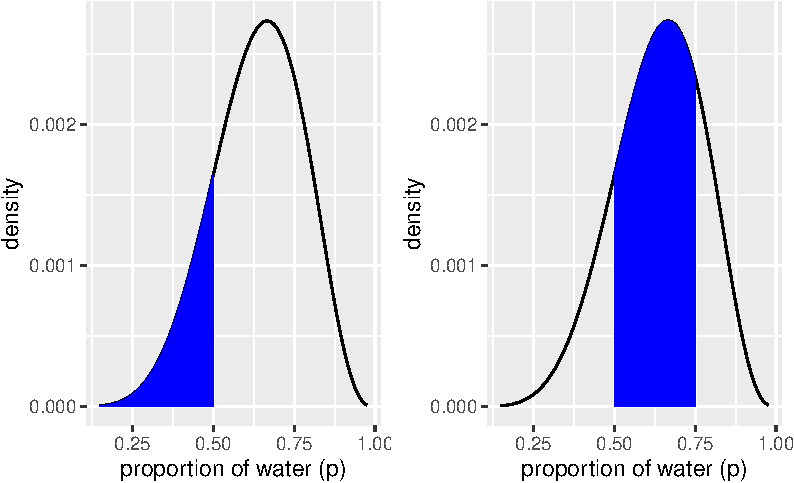
\includegraphics{03-sampling-the-imaginary_files/figure-pdf/fig-upper-part-3.2-1.pdf}

}

\caption{\label{fig-upper-part-3.2}Upper part of SR2 Figure 3.2:
Posterior distribution produced with \{\textbf{tidyverse}\} tools: Left:
The blue area is the posterior probability below a parameter value of
0.5. Right: The posterior probability between 0.5 and 0.75.}

\end{figure}

\hypertarget{intervals-of-defined-probability-mass}{%
\subsection{Intervals of Defined Probability
Mass}\label{intervals-of-defined-probability-mass}}

\hypertarget{original-12}{%
\subsubsection{Original}\label{original-12}}

\hypertarget{quantiles}{%
\paragraph{Quantiles}\label{quantiles}}

\begin{quote}
Reporting an interval of defined mass is usually known as a
\textbf{CONFIDENCE INTERVAL}. An interval of posterior probability, such
as the ones we are working with, may instead be called a
\textbf{CREDIBLE INTERVAL}.
\end{quote}

\begin{quote}
We're going to call it a \textbf{COMPATIBILITY INTERVAL} instead, in
order to avoid the unwarranted implications of ``confidence'' and
``credibility.'' What the interval indicates is a range of parameter
values compatible with the model and data. The model and data themselves
may not inspire confidence, in which case the interval will not either.
\end{quote}

\begin{quote}
For this type of interval, it is easier to find the answer by using
samples from the posterior than by using a grid approximation. Suppose
for example you want to know the boundaries of the lower 80\% posterior
probability. You know this interval starts at \(p = 0\). To find out
where it stops, think of the samples as data and ask where the 80th
percentile lies:
\end{quote}

\begin{Shaded}
\begin{Highlighting}[]
\InformationTok{\textasciigrave{}\textasciigrave{}\textasciigrave{}\{r\}}
\CommentTok{\#| label: samples{-}quantile{-}a}

\DocumentationTok{\#\# R code 3.9}
\FunctionTok{quantile}\NormalTok{(samples\_a, }\FloatTok{0.8}\NormalTok{)}
\InformationTok{\textasciigrave{}\textasciigrave{}\textasciigrave{}}
\end{Highlighting}
\end{Shaded}

\begin{verbatim}
#>       80% 
#> 0.7627628
\end{verbatim}

Similarly, the middle 80\% interval lies between the 10th percentile and
the 90th percentile. These boundaries are found using the same approach:

\begin{Shaded}
\begin{Highlighting}[]
\InformationTok{\textasciigrave{}\textasciigrave{}\textasciigrave{}\{r\}}
\CommentTok{\#| label: sample{-}quantile{-}a2}

\DocumentationTok{\#\# R code 3.10}
\FunctionTok{quantile}\NormalTok{(samples\_a, }\FunctionTok{c}\NormalTok{(}\FloatTok{0.1}\NormalTok{, }\FloatTok{0.9}\NormalTok{))}
\InformationTok{\textasciigrave{}\textasciigrave{}\textasciigrave{}}
\end{Highlighting}
\end{Shaded}

\begin{verbatim}
#>       10%       90% 
#> 0.4514515 0.8148148
\end{verbatim}

Intervals of this sort, which assign equal probability mass to each
tail, are very common in the scientific literature. We'll call them
\textbf{PERCENTILE INTERVALS} (PI). These intervals do a good job of
communicating the shape of a distribution, as long as the distribution
isn't too asymmetrical. But in terms of describing the shape of the
posterior distribution---which is really all these intervals are asked
to do---the percentile interval can be misleading.

Consider the posterior distribution and different intervals in
Picture~\ref{fig-skewed-dist-a}. This posterior is consistent with
observing three waters in three tosses and a uniform (flat) prior. It is
highly skewed, having its maximum value at the boundary, \(p = 1\). You
can compute it, via grid approximation.

\hypertarget{skewed-distribution}{%
\paragraph{Skewed distribution}\label{skewed-distribution}}

\begin{Shaded}
\begin{Highlighting}[]
\InformationTok{\textasciigrave{}\textasciigrave{}\textasciigrave{}\{r\}}
\CommentTok{\#| label: fig{-}skewed{-}dist{-}a}
\CommentTok{\#| fig{-}cap: "Skewed posterior distribution observing three waters in three tosses and a uniform (flat) prior. It is highly skewed, having its maximum value at the boundary where p equals 1."}

\DocumentationTok{\#\# R code 3.11}
\NormalTok{p\_grid\_skewed\_a }\OtherTok{\textless{}{-}} \FunctionTok{seq}\NormalTok{(}\AttributeTok{from =} \DecValTok{0}\NormalTok{, }\AttributeTok{to =} \DecValTok{1}\NormalTok{, }\AttributeTok{length.out =} \DecValTok{1000}\NormalTok{)}
\NormalTok{prior\_skewed\_a }\OtherTok{\textless{}{-}} \FunctionTok{rep}\NormalTok{(}\DecValTok{1}\NormalTok{, }\DecValTok{1000}\NormalTok{)}
\NormalTok{likelihood\_skewed\_a }\OtherTok{\textless{}{-}} \FunctionTok{dbinom}\NormalTok{(}\DecValTok{3}\NormalTok{, }\AttributeTok{size =} \DecValTok{3}\NormalTok{, }\AttributeTok{prob =}\NormalTok{ p\_grid\_skewed\_a)}
\NormalTok{posterior\_skewed\_a }\OtherTok{\textless{}{-}}\NormalTok{ likelihood\_skewed\_a }\SpecialCharTok{*}\NormalTok{ prior\_skewed\_a}
\NormalTok{posterior\_skewed\_a }\OtherTok{\textless{}{-}}\NormalTok{ posterior\_skewed\_a }\SpecialCharTok{/} \FunctionTok{sum}\NormalTok{(posterior\_skewed\_a)}

\FunctionTok{set.seed}\NormalTok{(}\DecValTok{3}\NormalTok{) }\CommentTok{\# added to make sampling distribution reproducible (pb)}
\NormalTok{samples\_skewed\_a }\OtherTok{\textless{}{-}} \FunctionTok{sample}\NormalTok{(p\_grid\_skewed\_a, }\AttributeTok{size =} \FloatTok{1e4}\NormalTok{, }\AttributeTok{replace =} \ConstantTok{TRUE}\NormalTok{, }\AttributeTok{prob =}\NormalTok{ posterior\_skewed\_a)}



\CommentTok{\# added to show the skewed posterior distribution (pb)}
\NormalTok{rethinking}\SpecialCharTok{::}\FunctionTok{dens}\NormalTok{(samples\_skewed\_a)}
\InformationTok{\textasciigrave{}\textasciigrave{}\textasciigrave{}}
\end{Highlighting}
\end{Shaded}

\begin{figure}[H]

{\centering 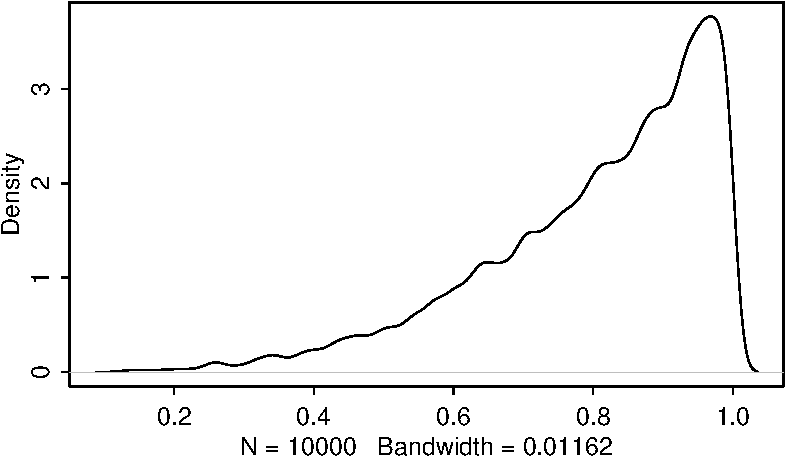
\includegraphics{03-sampling-the-imaginary_files/figure-pdf/fig-skewed-dist-a-1.pdf}

}

\caption{\label{fig-skewed-dist-a}Skewed posterior distribution
observing three waters in three tosses and a uniform (flat) prior. It is
highly skewed, having its maximum value at the boundary where p equals
1.}

\end{figure}

\hypertarget{percentile-compatibility-intervall-pi}{%
\paragraph{Percentile (compatibility) Intervall
(PI)}\label{percentile-compatibility-intervall-pi}}

\begin{Shaded}
\begin{Highlighting}[]
\InformationTok{\textasciigrave{}\textasciigrave{}\textasciigrave{}\{r\}}
\CommentTok{\#| label: rethinking{-}PI{-}a}

\DocumentationTok{\#\# R code 3.12}
\NormalTok{rethinking}\SpecialCharTok{::}\FunctionTok{PI}\NormalTok{(samples\_skewed\_a, }\AttributeTok{prob =} \FloatTok{0.5}\NormalTok{)}
\InformationTok{\textasciigrave{}\textasciigrave{}\textasciigrave{}}
\end{Highlighting}
\end{Shaded}

\begin{verbatim}
#>       25%       75% 
#> 0.7087087 0.9349349
\end{verbatim}

The Percentile compatibility Interval (PI) of \texttt{prob\ =\ 0.5}
assigns 25\% of the probability mass above and below the interval. So it
provides the central 50\% probability.

It is just a shorthand for the base R \texttt{stats::quantile()}
function:

\begin{Shaded}
\begin{Highlighting}[]
\InformationTok{\textasciigrave{}\textasciigrave{}\textasciigrave{}\{r\}}
\CommentTok{\#| label: quantiles{-}PI{-}a}

\FunctionTok{quantile}\NormalTok{(samples\_skewed\_a, }\AttributeTok{prob =} \FunctionTok{c}\NormalTok{(.}\DecValTok{25}\NormalTok{, .}\DecValTok{75}\NormalTok{))}
\InformationTok{\textasciigrave{}\textasciigrave{}\textasciigrave{}}
\end{Highlighting}
\end{Shaded}

\begin{verbatim}
#>       25%       75% 
#> 0.7087087 0.9349349
\end{verbatim}

\begin{quote}
This {[}percentile compability{]} interval assigns 25\% of the
probability mass above and below the interval. So it provides the
central 50\% probability. But in this example, it ends up excluding the
most probable parameter values, near \(p = 1\). So in terms of
describing the shape of the posterior distribution---which is really all
these intervals are asked to do---the percentile interval can be
misleading.
\end{quote}

To see how it works we make another PI of \texttt{prob\ =\ 0.6}. We
divide always the percentage by 2 and subtract it from 50\% respectively
add this value to 50\%. The result is the probability mass between
20-80\%.

\begin{Shaded}
\begin{Highlighting}[]
\InformationTok{\textasciigrave{}\textasciigrave{}\textasciigrave{}\{r\}}
\CommentTok{\#| label: rethinking{-}PI{-}a2}

\NormalTok{rethinking}\SpecialCharTok{::}\FunctionTok{PI}\NormalTok{(samples\_skewed\_a, }\AttributeTok{prob =} \FloatTok{0.6}\NormalTok{)}
\InformationTok{\textasciigrave{}\textasciigrave{}\textasciigrave{}}
\end{Highlighting}
\end{Shaded}

\begin{verbatim}
#>       20%       80% 
#> 0.6706707 0.9481481
\end{verbatim}

But in these examples, we end up excluding the most probable parameter
values, near \(p = 1\). So in terms of describing the shape of the
posterior distribution---which is really all these intervals are asked
to do---the percentile interval can be misleading.

\hypertarget{highest-posterior-density-interval-hpdi}{%
\paragraph{Highest Posterior Density Interval
(HPDI)}\label{highest-posterior-density-interval-hpdi}}

\begin{quote}
{[}In contrast, to PI the HPDI (HIGHEST POSTERIOR DENSITY INTERVAL){]}
displays the narrowest interval containing the specified probability
mass. If you think about it, there must be an infinite number of
posterior intervals with the same mass. But if you want an interval that
best represents the parameter values most consistent with the data, then
you want the densest of these intervals. That's what the HPDI is.
Compute it from the samples with HPDI (also part of rethinking):
\end{quote}

\begin{codelisting}

\caption{Compute the HPDI from the samples distribution}

\hypertarget{lst-rethinking-HPDI-a}{%
\label{lst-rethinking-HPDI-a}}%
\begin{Shaded}
\begin{Highlighting}[]
\InformationTok{\textasciigrave{}\textasciigrave{}\textasciigrave{}\{r\}}
\CommentTok{\#| label: rethinking{-}HPDI{-}a}
\CommentTok{\#| attr{-}source: \textquotesingle{}\#lst{-}rethinking{-}HPDI{-}a lst{-}cap="Compute the HPDI from the samples distribution"\textquotesingle{}}

\DocumentationTok{\#\# R code 3.13}
\NormalTok{rethinking}\SpecialCharTok{::}\FunctionTok{HPDI}\NormalTok{(samples\_skewed\_a, }\AttributeTok{prob =} \FloatTok{0.5}\NormalTok{)}
\InformationTok{\textasciigrave{}\textasciigrave{}\textasciigrave{}}
\end{Highlighting}
\end{Shaded}

\end{codelisting}

\begin{verbatim}
#>      |0.5      0.5| 
#> 0.8418418 0.9989990
\end{verbatim}

This interval captures the parameters with highest posterior
probability, as well as being noticeably narrower: 0.18 in width rather
than 0.28 for the percentile interval resp. 0.16 and 0.23 in the
original book version.

So the HPDI has some advantages over the PI. But in most cases, these
two types of interval are very similar. They only look so different in
this case because the posterior distribution is highly skewed. If we
instead used samples from the posterior distribution for six waters in
nine tosses, these intervals would be nearly identical. Try it for
yourself, using different probability masses, such as prob=0.8 and
prob=0.95.

\begin{Shaded}
\begin{Highlighting}[]
\InformationTok{\textasciigrave{}\textasciigrave{}\textasciigrave{}\{r\}}
\CommentTok{\#| label: PI{-}HPDI{-}in{-}sym{-}dist}

\NormalTok{rethinking}\SpecialCharTok{::}\FunctionTok{PI}\NormalTok{(samples\_a, }\AttributeTok{prob =} \FloatTok{0.8}\NormalTok{)}
\NormalTok{rethinking}\SpecialCharTok{::}\FunctionTok{HPDI}\NormalTok{(samples\_a, }\AttributeTok{prob =} \FloatTok{0.8}\NormalTok{)}

\NormalTok{rethinking}\SpecialCharTok{::}\FunctionTok{PI}\NormalTok{(samples\_a, }\AttributeTok{prob =} \FloatTok{0.95}\NormalTok{)}
\NormalTok{rethinking}\SpecialCharTok{::}\FunctionTok{HPDI}\NormalTok{(samples\_a, }\AttributeTok{prob =} \FloatTok{0.95}\NormalTok{)}
\InformationTok{\textasciigrave{}\textasciigrave{}\textasciigrave{}}
\end{Highlighting}
\end{Shaded}

\begin{verbatim}
#>       10%       90% 
#> 0.4514515 0.8148148 
#>      |0.8      0.8| 
#> 0.4874875 0.8448448 
#>        3%       98% 
#> 0.3493493 0.8788789 
#>     |0.95     0.95| 
#> 0.3703704 0.8938939
\end{verbatim}

\hypertarget{difference-between-pi-and-hdpi}{%
\paragraph{Difference between PI and
HDPI}\label{difference-between-pi-and-hdpi}}

\begin{quote}
When the posterior is bell shaped, it hardly matters which type of
interval you use. Remember, we're not launching rockets or calibrating
atom smashers, so fetishizing precision to the 5th decimal place will
not improve your science.
\end{quote}

\begin{quote}
The HPDI also has some disadvantages. HPDI is more computationally
intensive than PI and suffers from greater simulation variance, which is
a fancy way of saying that it is sensitive to how many samples you draw
from the posterior. It is also harder to understand and many scientific
audiences will not appreciate its features, while they will immediately
understand a percentile interval, as ordinary non-Bayesian intervals are
typically interpreted (incorrectly) as percentile intervals (although
see the Rethinking box below).
\end{quote}

\begin{quote}
Overall, if the choice of interval type makes a big difference, then you
shouldn't be using intervals to summarize the posterior. Remember, the
entire posterior distribution is the Bayesian ``estimate.'' It
summarizes the relative plausibilities of each possible value of the
parameter. Intervals of the distribution are just helpful for
summarizing it. If choice of interval leads to different inferences,
then you'd be better off just plotting the entire posterior
distribution.
\end{quote}

\hypertarget{intervall-mass-of-95}{%
\paragraph{Intervall mass of 95?}\label{intervall-mass-of-95}}

\begin{quote}
The most common interval mass in the natural and social sciences is the
95\% interval. This interval leaves 5\% of the probability outside,
corresponding to a 5\% chance of the parameter not lying within the
interval (although see below). This customary interval also reflects the
customary threshold for statistical significance, which is 5\% or p
\textless{} 0.05.
\end{quote}

It is just a convention, there are no analytical reasons why you should
choose exactly this interval. But convenience is not a serious
criterion. So what to do instead?

\begin{quote}
If you are trying to say that an interval doesn't include some value,
then you might use the widest interval that excludes the value. Often,
all compatibility intervals do is communicate the shape of a
distribution. In that case, a series of nested intervals may be more
useful than any one interval. For example, why not present 67\%, 89\%,
and 97\% intervals, along with the median? Why these values? No reason.
They are prime numbers, which makes them easy to remember. But all that
matters is they be spaced enough to illustrate the shape of the
posterior. And these values avoid 95\%, since conventional 95\%
intervals encourage many readers to conduct unconscious hypothesis
tests.
\end{quote}

\hypertarget{defined-boundaries-and-probabilty-mass}{%
\paragraph{Defined boundaries and probabilty
mass}\label{defined-boundaries-and-probabilty-mass}}

The difference between intervals of defined boundaries and intervals of
defined probability mass is that in the first case we ask for a
\textbf{probability of frequencies} whereas in the second case we
calculate a specified \textbf{amount of posterior probability}. As
result from the first question we get the percentage of the probability
whereas the result of the second question is the probability value of
the percentage of frequencies looked for.

The boundary intervals are grounded on the prob values (\(0-1\)) and
results in the percentage of the probability whereas the probability
mass intervals focus on the percentage of probabilities (\(0-100\)\%)
and results in probability values.

\hypertarget{tidyverse-12}{%
\subsubsection{Tidyverse}\label{tidyverse-12}}

\hypertarget{quantiles-1}{%
\paragraph{Quantiles}\label{quantiles-1}}

Since we saved our \texttt{samples\_b} samples within the well-named
\texttt{samples\_b} tibble, we'll have to index with \texttt{\$} within
\texttt{stats::quantile()}.

\begin{Shaded}
\begin{Highlighting}[]
\InformationTok{\textasciigrave{}\textasciigrave{}\textasciigrave{}\{r\}}
\CommentTok{\#| label: sample{-}quantile{-}b}

\NormalTok{(q80 }\OtherTok{\textless{}{-}} \FunctionTok{quantile}\NormalTok{(samples\_b}\SpecialCharTok{$}\NormalTok{samples\_b, }\AttributeTok{probs =}\NormalTok{ .}\DecValTok{8}\NormalTok{))}
\InformationTok{\textasciigrave{}\textasciigrave{}\textasciigrave{}}
\end{Highlighting}
\end{Shaded}

\begin{verbatim}
#>       80% 
#> 0.7627628
\end{verbatim}

For an alternative approach, we could \texttt{dplyr::select()} the
\texttt{samples\_b} vector, extract it from the tibble with
\texttt{dplyr::pull()}, and then pump it into
\texttt{stats::quantile()}.

\begin{quote}
\texttt{pull()} is similar to \texttt{\$}. It's mostly useful because it
looks a little nicer in pipes, it also works with remote data frames,
and it can optionally name the output.
\end{quote}

\begin{Shaded}
\begin{Highlighting}[]
\InformationTok{\textasciigrave{}\textasciigrave{}\textasciigrave{}\{r\}}
\CommentTok{\#| label: sample{-}quantile{-}b2}

\NormalTok{samples\_b }\SpecialCharTok{|\textgreater{}} 
    \FunctionTok{pull}\NormalTok{(samples\_b) }\SpecialCharTok{|\textgreater{}} 
    \FunctionTok{quantile}\NormalTok{(}\AttributeTok{probs =}\NormalTok{ .}\DecValTok{8}\NormalTok{)}
    
\InformationTok{\textasciigrave{}\textasciigrave{}\textasciigrave{}}
\end{Highlighting}
\end{Shaded}

\begin{verbatim}
#>       80% 
#> 0.7627628
\end{verbatim}

We might also use \texttt{stats::quantile()} within
\texttt{dplyr::summarise()}.

\begin{Shaded}
\begin{Highlighting}[]
\InformationTok{\textasciigrave{}\textasciigrave{}\textasciigrave{}\{r\}}
\CommentTok{\#| label: sample{-}quantile{-}b3}

\NormalTok{samples\_b }\SpecialCharTok{|\textgreater{}} 
    \FunctionTok{summarize}\NormalTok{(}\AttributeTok{q80\_2 =} \FunctionTok{quantile}\NormalTok{(samples\_b, }\AttributeTok{probs =}\NormalTok{ .}\DecValTok{8}\NormalTok{))}
\InformationTok{\textasciigrave{}\textasciigrave{}\textasciigrave{}}
\end{Highlighting}
\end{Shaded}

\begin{verbatim}
#> # A tibble: 1 x 1
#>   q80_2
#>   <dbl>
#> 1 0.763
\end{verbatim}

Here's the \texttt{summarise()} approach with two probabilities.

\begin{Shaded}
\begin{Highlighting}[]
\InformationTok{\textasciigrave{}\textasciigrave{}\textasciigrave{}\{r\}}
\CommentTok{\#| label: sample{-}quantile{-}b4}

\NormalTok{samples\_b }\SpecialCharTok{|\textgreater{}} 
    \FunctionTok{summarize}\NormalTok{(}\AttributeTok{q10 =} \FunctionTok{quantile}\NormalTok{(samples\_b, }\AttributeTok{probs =}\NormalTok{ .}\DecValTok{1}\NormalTok{),}
              \AttributeTok{q90 =} \FunctionTok{quantile}\NormalTok{(samples\_b, }\AttributeTok{probs =}\NormalTok{ .}\DecValTok{9}\NormalTok{))}
    
\InformationTok{\textasciigrave{}\textasciigrave{}\textasciigrave{}}
\end{Highlighting}
\end{Shaded}

\begin{verbatim}
#> # A tibble: 1 x 2
#>     q10   q90
#>   <dbl> <dbl>
#> 1 0.451 0.815
\end{verbatim}

You can also use the vector feature of R to summarize different
quantiles with one line. But Kurz's version is in the meanwhile
deprecated:

\begin{Shaded}
\begin{Highlighting}[]
\InformationTok{\textasciigrave{}\textasciigrave{}\textasciigrave{}\{r\}}
\CommentTok{\#| label: sample{-}quantile{-}b5}

\NormalTok{samples\_b }\SpecialCharTok{|\textgreater{}} 
    \FunctionTok{summarize}\NormalTok{(}\AttributeTok{q10\_90 =} \FunctionTok{quantile}\NormalTok{(samples\_b, }\AttributeTok{probs =} \FunctionTok{c}\NormalTok{(.}\DecValTok{1}\NormalTok{, .}\DecValTok{9}\NormalTok{)))}
\InformationTok{\textasciigrave{}\textasciigrave{}\textasciigrave{}}
\end{Highlighting}
\end{Shaded}

\begin{verbatim}
#> Warning: Returning more (or less) than 1 row per `summarise()` group was deprecated in
#> dplyr 1.1.0.
#> i Please use `reframe()` instead.
#> i When switching from `summarise()` to `reframe()`, remember that `reframe()`
#>   always returns an ungrouped data frame and adjust accordingly.
#> # A tibble: 2 x 1
#>   q10_90
#>    <dbl>
#> 1  0.451
#> 2  0.815
\end{verbatim}

\begin{Shaded}
\begin{Highlighting}[]
\InformationTok{\textasciigrave{}\textasciigrave{}\textasciigrave{}\{r\}}
\CommentTok{\#| label: sample{-}quantile{-}b6}

\NormalTok{samples\_b }\SpecialCharTok{|\textgreater{}} 
    \FunctionTok{reframe}\NormalTok{(}\AttributeTok{q10\_90 =} \FunctionTok{quantile}\NormalTok{(samples\_b, }\AttributeTok{probs =} \FunctionTok{c}\NormalTok{(.}\DecValTok{1}\NormalTok{, .}\DecValTok{9}\NormalTok{)))}
\InformationTok{\textasciigrave{}\textasciigrave{}\textasciigrave{}}
\end{Highlighting}
\end{Shaded}

\begin{verbatim}
#> # A tibble: 2 x 1
#>   q10_90
#>    <dbl>
#> 1  0.451
#> 2  0.815
\end{verbatim}

From the help file of \texttt{dplyr::reframe()}:

\begin{quote}
While \texttt{summarise()} requires that each argument returns a single
value, and \texttt{mutate()} requires that each argument returns the
same number of rows as the input, \texttt{reframe()} is a more general
workhorse with no requirements on the number of rows returned per group.

\texttt{reframe()} creates a new data frame by applying functions to
columns of an existing data frame. It is most similar to
\texttt{summarise()}, with two big differences:

\begin{itemize}
\tightlist
\item
  \texttt{reframe()} can return an arbitrary number of rows per group,
  while \texttt{summarise()} reduces each group down to a single row.
\item
  \texttt{reframe()} always returns an ungrouped data frame, while
  \texttt{summarise()} might return a grouped or rowwise data frame,
  depending on the scenario.
\end{itemize}

We expect that you'll use \texttt{summarise()} much more often than
\texttt{reframe()}, but \texttt{reframe()} can be particularly helpful
when you need to apply a complex function that doesn't return a single
summary value.
\end{quote}

See also the appropriate
\href{https://www.tidyverse.org/blog/2023/02/dplyr-1-1-0-pick-reframe-arrange/\#reframe}{section
in the blog post} about changes in \{\textbf{dplyr}\} 1.1.0. The name
\texttt{reframe()} is in accordance with \texttt{tibble::enframe()} and
\texttt{tibble::deframe()}:

\begin{itemize}
\tightlist
\item
  \texttt{enframe()}: Takes a vector, returns a data frame
\item
  \texttt{deframe()}: Takes a data frame, returns a vector
\item
  \texttt{reframe()}: Takes a data frame, returns a data frame
\end{itemize}

\begin{quote}
The functions of the tidyverse approach typically returns a data frame.
But sometimes you just want your values in a numeric vector for the sake
of quick indexing. In that case, base R \texttt{stats::quantile()}
shines:
\end{quote}

\begin{Shaded}
\begin{Highlighting}[]
\InformationTok{\textasciigrave{}\textasciigrave{}\textasciigrave{}\{r\}}
\CommentTok{\#| label: sample{-}quantile{-}b7}

\NormalTok{(}\AttributeTok{q10\_q90 =} \FunctionTok{quantile}\NormalTok{(samples\_b}\SpecialCharTok{$}\NormalTok{samples\_b, }\AttributeTok{probs =} \FunctionTok{c}\NormalTok{(.}\DecValTok{1}\NormalTok{, .}\DecValTok{9}\NormalTok{)))}
\InformationTok{\textasciigrave{}\textasciigrave{}\textasciigrave{}}
\end{Highlighting}
\end{Shaded}

\begin{verbatim}
#>       10%       90% 
#> 0.4514515 0.8148148
\end{verbatim}

\hypertarget{plot-intervals-of-defined-mass}{%
\paragraph{Plot intervals of defined
mass}\label{plot-intervals-of-defined-mass}}

Now we have our cutoff values saved as \texttt{q80}, respectively
\texttt{q10} and \texttt{q90}, we're ready to make the bottom panels of
Figure 3.2.

\begin{Shaded}
\begin{Highlighting}[]
\InformationTok{\textasciigrave{}\textasciigrave{}\textasciigrave{}\{r\}}
\CommentTok{\#| label: figure{-}3{-}2{-}lower{-}part}

\NormalTok{p1 }\OtherTok{\textless{}{-}}
\NormalTok{  samples\_b }\SpecialCharTok{\%\textgreater{}\%} 
  \FunctionTok{ggplot}\NormalTok{(}\FunctionTok{aes}\NormalTok{(}\AttributeTok{x =}\NormalTok{ samples\_b, }\AttributeTok{y =}\NormalTok{ posterior\_samples\_b)) }\SpecialCharTok{+}
  \FunctionTok{geom\_line}\NormalTok{() }\SpecialCharTok{+}
  \FunctionTok{geom\_area}\NormalTok{(}\AttributeTok{data =}\NormalTok{ samples\_b }\SpecialCharTok{\%\textgreater{}\%} \FunctionTok{filter}\NormalTok{(samples\_b }\SpecialCharTok{\textless{}}\NormalTok{ q80), }\AttributeTok{fill =} \StringTok{"blue"}\NormalTok{) }\SpecialCharTok{+}
  \FunctionTok{annotate}\NormalTok{(}\AttributeTok{geom =} \StringTok{"text"}\NormalTok{,}
           \AttributeTok{x =}\NormalTok{ .}\DecValTok{25}\NormalTok{, }\AttributeTok{y =}\NormalTok{ .}\DecValTok{0025}\NormalTok{,}
           \AttributeTok{label =} \StringTok{"lower 80\%"}\NormalTok{) }\SpecialCharTok{+}
  \FunctionTok{labs}\NormalTok{(}\AttributeTok{x =} \StringTok{"proportion of water (p)"}\NormalTok{,}
       \AttributeTok{y =} \StringTok{"density"}\NormalTok{)}

\CommentTok{\# upper right panel}
\NormalTok{p2 }\OtherTok{\textless{}{-}} 
\NormalTok{  samples\_b }\SpecialCharTok{\%\textgreater{}\%} 
  \FunctionTok{ggplot}\NormalTok{(}\FunctionTok{aes}\NormalTok{(}\AttributeTok{x =}\NormalTok{ samples\_b, }\AttributeTok{y =}\NormalTok{ posterior\_samples\_b)) }\SpecialCharTok{+}
  \FunctionTok{geom\_line}\NormalTok{() }\SpecialCharTok{+}
  \FunctionTok{geom\_area}\NormalTok{(}\AttributeTok{data =}\NormalTok{ samples\_b }\SpecialCharTok{\%\textgreater{}\%} \FunctionTok{filter}\NormalTok{(samples\_b }\SpecialCharTok{\textgreater{}}\NormalTok{ q10\_q90[[}\DecValTok{1}\NormalTok{]] }\SpecialCharTok{\&}\NormalTok{ samples\_b }\SpecialCharTok{\textless{}}\NormalTok{ q10\_q90[[}\DecValTok{2}\NormalTok{]]), }\AttributeTok{fill =} \StringTok{"blue"}\NormalTok{) }\SpecialCharTok{+}
  \FunctionTok{annotate}\NormalTok{(}\AttributeTok{geom =} \StringTok{"text"}\NormalTok{,}
           \AttributeTok{x =}\NormalTok{ .}\DecValTok{25}\NormalTok{, }\AttributeTok{y =}\NormalTok{ .}\DecValTok{0025}\NormalTok{,}
           \AttributeTok{label =} \StringTok{"middle 80\%"}\NormalTok{) }\SpecialCharTok{+}
  \FunctionTok{labs}\NormalTok{(}\AttributeTok{x =} \StringTok{"proportion of water (p)"}\NormalTok{,}
       \AttributeTok{y =} \StringTok{"density"}\NormalTok{)}

\FunctionTok{library}\NormalTok{(patchwork)}
\NormalTok{p1 }\SpecialCharTok{+}\NormalTok{ p2}
\InformationTok{\textasciigrave{}\textasciigrave{}\textasciigrave{}}
\end{Highlighting}
\end{Shaded}

\begin{figure}[H]

{\centering 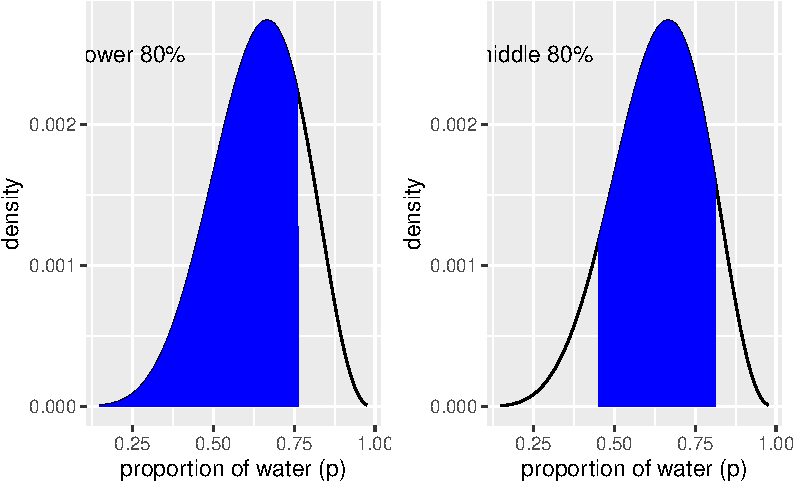
\includegraphics{03-sampling-the-imaginary_files/figure-pdf/figure-3-2-lower-part-1.pdf}

}

\end{figure}

\hypertarget{skewed-distribution-1}{%
\paragraph{Skewed distribution}\label{skewed-distribution-1}}

Again we will demonstrate the misleading character of Pecentile
Intervals (PIs) with a very skewed distribution.

We've already defined \texttt{p\_grid\_b} and \texttt{prior\_b} within
\texttt{d\_b}, above. Here we'll reuse them and create a new tibble by
updating all the columns with the skewed parameters.

\begin{Shaded}
\begin{Highlighting}[]
\InformationTok{\textasciigrave{}\textasciigrave{}\textasciigrave{}\{r\}}
\CommentTok{\#| label: samples{-}skewed{-}dist}

\NormalTok{n\_samples\_skewed\_b }\OtherTok{\textless{}{-}} \FloatTok{1e4}
\NormalTok{n\_success\_skewed\_b }\OtherTok{\textless{}{-}} \DecValTok{3}
\NormalTok{n\_trials\_skewed\_b  }\OtherTok{\textless{}{-}} \DecValTok{3}

\NormalTok{d\_skewed\_b }\OtherTok{\textless{}{-}}
\FunctionTok{tibble}\NormalTok{(}\AttributeTok{p\_grid\_skewed\_b =} \FunctionTok{seq}\NormalTok{(}\AttributeTok{from =} \DecValTok{0}\NormalTok{, }\AttributeTok{to =} \DecValTok{1}\NormalTok{, }\AttributeTok{length.out =}\NormalTok{ n\_samples\_skewed\_b),}
     \CommentTok{\# note we\textquotesingle{}re still using a flat uniform prior}
     \AttributeTok{prior\_skewed\_b  =} \DecValTok{1}\NormalTok{) }\SpecialCharTok{\%\textgreater{}\%} 
\FunctionTok{mutate}\NormalTok{(}\AttributeTok{likelihood\_skewed\_b =} \FunctionTok{dbinom}\NormalTok{(n\_success\_skewed\_b, }\AttributeTok{size =}\NormalTok{ n\_trials\_skewed\_b, }\AttributeTok{prob =}\NormalTok{ p\_grid\_skewed\_b)) }\SpecialCharTok{\%\textgreater{}\%} 
\FunctionTok{mutate}\NormalTok{(}\AttributeTok{posterior\_skewed\_b =}\NormalTok{ (likelihood\_skewed\_b }\SpecialCharTok{*}\NormalTok{ prior\_skewed\_b) }\SpecialCharTok{/} \FunctionTok{sum}\NormalTok{(likelihood\_skewed\_b }\SpecialCharTok{*}\NormalTok{ prior\_skewed\_b))}

\CommentTok{\# make the next part reproducible}
\FunctionTok{set.seed}\NormalTok{(}\DecValTok{3}\NormalTok{)}

\CommentTok{\# here\textquotesingle{}s our new samples tibble}
\NormalTok{(}
\NormalTok{  samples\_skewed\_b }\OtherTok{\textless{}{-}}
\NormalTok{    d\_skewed\_b }\SpecialCharTok{\%\textgreater{}\%} 
    \FunctionTok{slice\_sample}\NormalTok{(}\AttributeTok{n =}\NormalTok{ n\_samples\_skewed\_b, }\AttributeTok{weight\_by =}\NormalTok{ posterior\_skewed\_b, }\AttributeTok{replace =}\NormalTok{ T)}
\NormalTok{)}
\InformationTok{\textasciigrave{}\textasciigrave{}\textasciigrave{}}
\end{Highlighting}
\end{Shaded}

\begin{verbatim}
#> # A tibble: 10,000 x 4
#>    p_grid_skewed_b prior_skewed_b likelihood_skewed_b posterior_skewed_b
#>              <dbl>          <dbl>               <dbl>              <dbl>
#>  1           0.874              1               0.669          0.000267 
#>  2           0.830              1               0.572          0.000229 
#>  3           0.684              1               0.320          0.000128 
#>  4           0.903              1               0.735          0.000294 
#>  5           0.750              1               0.423          0.000169 
#>  6           0.989              1               0.968          0.000387 
#>  7           0.875              1               0.670          0.000268 
#>  8           0.522              1               0.143          0.0000570
#>  9           0.967              1               0.903          0.000361 
#> 10           0.967              1               0.903          0.000361 
#> # i 9,990 more rows
\end{verbatim}

\begin{Shaded}
\begin{Highlighting}[]
\InformationTok{\textasciigrave{}\textasciigrave{}\textasciigrave{}\{r\}}
\CommentTok{\#| label: skewed{-}dist{-}b}


\CommentTok{\# here we update the \textasciigrave{}dbinom()\textasciigrave{} parameters }
\CommentTok{\# for values for a skewed distribution}
\CommentTok{\# assuming three trials results in 3 W (Water)}
\NormalTok{n\_success\_skewed\_b }\OtherTok{\textless{}{-}} \DecValTok{3}
\NormalTok{n\_trials\_skewed\_b  }\OtherTok{\textless{}{-}} \DecValTok{3}

\CommentTok{\# update \textasciigrave{}d\_b\textasciigrave{} to d\_skewed\_b}
\NormalTok{d\_skewed\_b }\OtherTok{\textless{}{-}}
\NormalTok{  d\_b }\SpecialCharTok{\%\textgreater{}\%} 
  \FunctionTok{mutate}\NormalTok{(}\AttributeTok{likelihood\_skewed\_b =} \FunctionTok{dbinom}\NormalTok{(n\_success\_skewed\_b, }\AttributeTok{size =}\NormalTok{ n\_trials\_skewed\_b, }\AttributeTok{prob =}\NormalTok{ p\_grid\_b)) }\SpecialCharTok{\%\textgreater{}\%} 
  \FunctionTok{mutate}\NormalTok{(}\AttributeTok{posterior\_skewed\_b  =}\NormalTok{ (likelihood\_skewed\_b }\SpecialCharTok{*}\NormalTok{ prior\_b) }\SpecialCharTok{/} \FunctionTok{sum}\NormalTok{(likelihood\_skewed\_b }\SpecialCharTok{*}\NormalTok{ prior\_b))}

\CommentTok{\# make the next part reproducible}
\FunctionTok{set.seed}\NormalTok{(}\DecValTok{3}\NormalTok{)}

\CommentTok{\# here\textquotesingle{}s our new samples tibble}
\NormalTok{(}
\NormalTok{    samples\_skewed\_b }\OtherTok{\textless{}{-}} 
\NormalTok{        d\_skewed\_b }\SpecialCharTok{\%\textgreater{}\%} 
        \FunctionTok{slice\_sample}\NormalTok{(}\AttributeTok{n =}\NormalTok{ n\_samples\_skewed\_b, }\AttributeTok{weight\_by =}\NormalTok{ posterior\_skewed\_b, }\AttributeTok{replace =}\NormalTok{ T) }\SpecialCharTok{|\textgreater{}} 
        \FunctionTok{rename}\NormalTok{(}\AttributeTok{p\_skewed\_b =}\NormalTok{ p\_grid\_b,}
               \AttributeTok{prior\_skewed\_b =}\NormalTok{ prior\_b)}
\NormalTok{)}

\CommentTok{\# added to see the skewed distribution}
\NormalTok{samples\_skewed\_b }\SpecialCharTok{\%\textgreater{}\%} 
  \FunctionTok{ggplot}\NormalTok{(}\FunctionTok{aes}\NormalTok{(}\AttributeTok{x =}\NormalTok{ p\_skewed\_b, }\AttributeTok{y =}\NormalTok{ posterior\_skewed\_b)) }\SpecialCharTok{+}
  \FunctionTok{geom\_line}\NormalTok{()}
\InformationTok{\textasciigrave{}\textasciigrave{}\textasciigrave{}}
\end{Highlighting}
\end{Shaded}

\begin{verbatim}
#> # A tibble: 10,000 x 6
#>    p_skewed_b prior_skewed_b likelihood_b posterior_b likelihood_skewed_b
#>         <dbl>          <dbl>        <dbl>       <dbl>               <dbl>
#>  1      0.717              1    0.259     0.00259                  0.368 
#>  2      0.652              1    0.272     0.00272                  0.277 
#>  3      0.548              1    0.210     0.00210                  0.164 
#>  4      1                  1    0         0                        1     
#>  5      0.991              1    0.0000582 0.000000582              0.973 
#>  6      0.788              1    0.192     0.00192                  0.489 
#>  7      0.940              1    0.0125    0.000126                 0.830 
#>  8      0.817              1    0.153     0.00154                  0.545 
#>  9      0.955              1    0.00582   0.0000583                0.871 
#> 10      0.449              1    0.116     0.00116                  0.0908
#> # i 9,990 more rows
#> # i 1 more variable: posterior_skewed_b <dbl>
\end{verbatim}

\begin{figure}[H]

{\centering 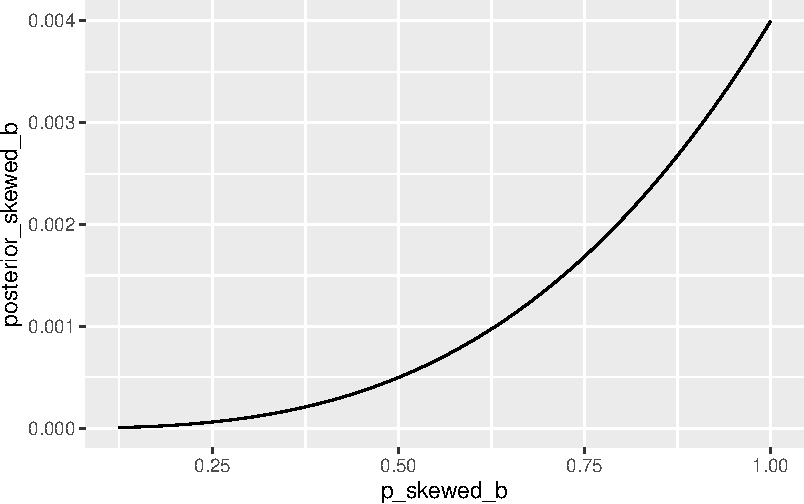
\includegraphics{03-sampling-the-imaginary_files/figure-pdf/skewed-dist-b-1.pdf}

}

\end{figure}

\hypertarget{reconsideration-2}{%
\paragraph{Reconsideration}\label{reconsideration-2}}

To see the difference how the skewed distribution is different to the
Figure 3.2 lower part, I will draw the appropriate figure here myself.

\begin{Shaded}
\begin{Highlighting}[]
\InformationTok{\textasciigrave{}\textasciigrave{}\textasciigrave{}\{r\}}
\CommentTok{\#| label: figure{-}3.2{-}skewed{-}lower{-}part}

\NormalTok{p1 }\OtherTok{\textless{}{-}}
\NormalTok{  samples\_skewed\_b }\SpecialCharTok{\%\textgreater{}\%} 
  \FunctionTok{ggplot}\NormalTok{(}\FunctionTok{aes}\NormalTok{(}\AttributeTok{x =}\NormalTok{ p\_skewed\_b, }\AttributeTok{y =}\NormalTok{ posterior\_skewed\_b)) }\SpecialCharTok{+}
  \FunctionTok{geom\_line}\NormalTok{() }\SpecialCharTok{+}
  \FunctionTok{geom\_area}\NormalTok{(}\AttributeTok{data =}\NormalTok{ samples\_skewed\_b }\SpecialCharTok{\%\textgreater{}\%} \FunctionTok{filter}\NormalTok{(p\_skewed\_b }\SpecialCharTok{\textless{}}\NormalTok{ q80), }\AttributeTok{fill =} \StringTok{"blue"}\NormalTok{) }\SpecialCharTok{+}
  \FunctionTok{annotate}\NormalTok{(}\AttributeTok{geom =} \StringTok{"text"}\NormalTok{,}
           \AttributeTok{x =}\NormalTok{ .}\DecValTok{25}\NormalTok{, }\AttributeTok{y =}\NormalTok{ .}\DecValTok{0025}\NormalTok{,}
           \AttributeTok{label =} \StringTok{"lower 80\%"}\NormalTok{) }\SpecialCharTok{+}
  \FunctionTok{labs}\NormalTok{(}\AttributeTok{x =} \StringTok{"proportion of water (p)"}\NormalTok{,}
       \AttributeTok{y =} \StringTok{"density"}\NormalTok{)}

\CommentTok{\# upper right panel}
\NormalTok{p2 }\OtherTok{\textless{}{-}} 
\NormalTok{  samples\_skewed\_b }\SpecialCharTok{\%\textgreater{}\%} 
  \FunctionTok{ggplot}\NormalTok{(}\FunctionTok{aes}\NormalTok{(}\AttributeTok{x =}\NormalTok{ p\_skewed\_b, }\AttributeTok{y =}\NormalTok{ posterior\_skewed\_b)) }\SpecialCharTok{+}
  \FunctionTok{geom\_line}\NormalTok{() }\SpecialCharTok{+}
  \FunctionTok{geom\_area}\NormalTok{(}\AttributeTok{data =}\NormalTok{ samples\_skewed\_b }\SpecialCharTok{\%\textgreater{}\%} \FunctionTok{filter}\NormalTok{(p\_skewed\_b }\SpecialCharTok{\textgreater{}}\NormalTok{ q10\_q90[[}\DecValTok{1}\NormalTok{]] }\SpecialCharTok{\&}\NormalTok{ p\_skewed\_b }\SpecialCharTok{\textless{}}\NormalTok{ q10\_q90[[}\DecValTok{2}\NormalTok{]]), }\AttributeTok{fill =} \StringTok{"blue"}\NormalTok{) }\SpecialCharTok{+}
  \FunctionTok{annotate}\NormalTok{(}\AttributeTok{geom =} \StringTok{"text"}\NormalTok{,}
           \AttributeTok{x =}\NormalTok{ .}\DecValTok{25}\NormalTok{, }\AttributeTok{y =}\NormalTok{ .}\DecValTok{0025}\NormalTok{,}
           \AttributeTok{label =} \StringTok{"middle 80\%"}\NormalTok{) }\SpecialCharTok{+}
  \FunctionTok{labs}\NormalTok{(}\AttributeTok{x =} \StringTok{"proportion of water (p)"}\NormalTok{,}
       \AttributeTok{y =} \StringTok{"density"}\NormalTok{)}

\FunctionTok{library}\NormalTok{(patchwork)}
\NormalTok{p1 }\SpecialCharTok{+}\NormalTok{ p2}
\InformationTok{\textasciigrave{}\textasciigrave{}\textasciigrave{}}
\end{Highlighting}
\end{Shaded}

\begin{figure}[H]

{\centering 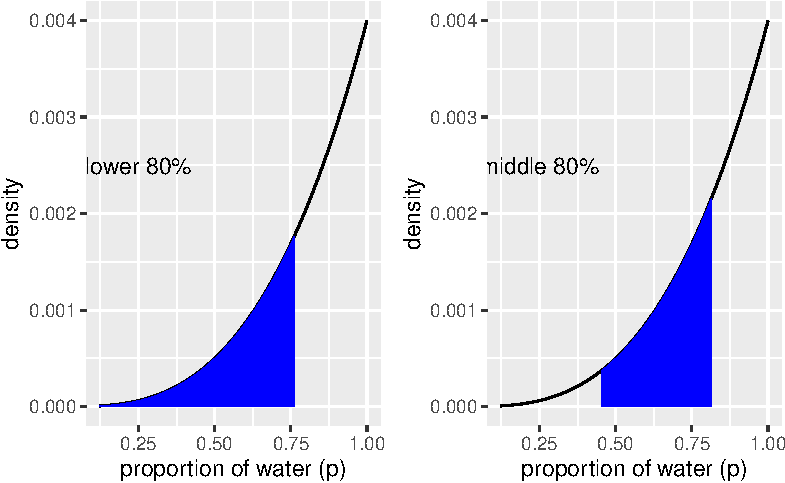
\includegraphics{03-sampling-the-imaginary_files/figure-pdf/figure-3.2-skewed-lower-part-1.pdf}

}

\end{figure}

\hypertarget{introducing-tidybayes}{%
\paragraph{Introducing tidybayes}\label{introducing-tidybayes}}

The \href{https://mjskay.github.io/tidybayes/}{\{\textbf{tidybayes}\}}
package offers an array of convenience functions for summarizing
Bayesian models. For an introduction using \{\textbf{tidybayes}\} with
\{\textbf{brms}\} see
\href{https://mjskay.github.io/tidybayes/articles/tidy-brms.html}{Extracting
and visualizing tidy draws from \{\textbf{brms}\} models}.

\begin{quote}
\{\textbf{tidybayes}\} is an R package that aims to make it easy to
integrate popular Bayesian modeling methods into a tidy data + ggplot
workflow. It builds on top of (and re-exports) several functions for
visualizing uncertainty from its sister package,
\href{https://mjskay.github.io/ggdist/}{\{\textbf{ggdist}\}}.
\end{quote}

I had difficulties to use Kurz's functions because there was an
\href{https://mjskay.github.io/tidybayes/reference/tidybayes-deprecated.html}{overhaul
in the naming scheme} of \{\textbf{tidybayes}\} version 1.0 and a
deprecation of horizontal shortcut geoms and stats in
\{\textbf{tidybayes}\} 2.1. Because \{\textbf{tidybayes}\} integrates
function of the sister package \{\textbf{ggdist}\} the
\href{https://mjskay.github.io/ggdist/reference/index.html}{function
descriptions and references of \{\textbf{ggdist}\}} are also important
to consult.

For the following parts the section on
\href{https://mjskay.github.io/tidybayes/articles/tidy-brms.html\#point-summaries-and-intervals}{Point
Summaries and Intervals} and the reference on
\href{https://mjskay.github.io/ggdist/reference/point_interval.html}{Point
and interval summaries for tidy data frames of draws from distributions}
are especially important.

The \{\textbf{tidybayes}\} package contains a
\href{https://mjskay.github.io/tidybayes/articles/tidy-brms.html\#point-summaries-and-intervals}{family
of functions} that make it easy to summarize a distribution with a
measure of central tendency accompanied by intervals. With
\texttt{tidybayes::median\_qi()}, we will ask for the median and
quantile-based intervals --- just like we've been doing with
\texttt{stats::quantile()}.

\begin{tcolorbox}[enhanced jigsaw, colframe=quarto-callout-caution-color-frame, colback=white, toprule=.15mm, breakable, arc=.35mm, bottomtitle=1mm, colbacktitle=quarto-callout-caution-color!10!white, toptitle=1mm, titlerule=0mm, title=\textcolor{quarto-callout-caution-color}{\faFire}\hspace{0.5em}{Caution}, leftrule=.75mm, opacityback=0, rightrule=.15mm, opacitybacktitle=0.6, bottomrule=.15mm, left=2mm, coltitle=black]

Although Kurz uses the \texttt{samples} data frame I cannot reproduce it
with \texttt{samples\_b} data frame, because has changed it values
recently to the skewed sampling version. To get the same results as Kurz
I have to use in my naming scheme the \texttt{skewed} version.

\end{tcolorbox}

\begin{Shaded}
\begin{Highlighting}[]
\InformationTok{\textasciigrave{}\textasciigrave{}\textasciigrave{}\{r\}}
\CommentTok{\#| label: median{-}quantile{-}interval}

\NormalTok{tidybayes}\SpecialCharTok{::}\FunctionTok{median\_qi}\NormalTok{(samples\_skewed\_b}\SpecialCharTok{$}\NormalTok{p\_skewed\_b, }\AttributeTok{.width =}\NormalTok{ .}\DecValTok{5}\NormalTok{)}
\InformationTok{\textasciigrave{}\textasciigrave{}\textasciigrave{}}
\end{Highlighting}
\end{Shaded}

\begin{verbatim}
#>           y      ymin      ymax .width .point .interval
#> 1 0.8428428 0.7087087 0.9349349    0.5 median        qi
\end{verbatim}

Note how the \texttt{.width} argument within
\texttt{tidybayes::median\_qi()} worked the same way the \texttt{prob}
argument did within \texttt{rethinking::PI()}. With
\texttt{.width\ =\ .5}, we indicated we wanted a quantile-based 50\%
interval, which was returned in the \texttt{ymin} and \texttt{ymax}
columns.

The \{\textbf{tidybayes}\} framework makes it easy to request multiple
types of intervals. In the following code chunk we'll request 50\%,
80\%, and 99\% intervals.

\begin{Shaded}
\begin{Highlighting}[]
\InformationTok{\textasciigrave{}\textasciigrave{}\textasciigrave{}\{r\}}
\CommentTok{\#| label: multiple{-}intervals}

\NormalTok{tidybayes}\SpecialCharTok{::}\FunctionTok{median\_qi}\NormalTok{(samples\_skewed\_b}\SpecialCharTok{$}\NormalTok{p\_skewed\_b, }\AttributeTok{.width =} \FunctionTok{c}\NormalTok{(.}\DecValTok{5}\NormalTok{, .}\DecValTok{8}\NormalTok{, .}\DecValTok{99}\NormalTok{))}
\InformationTok{\textasciigrave{}\textasciigrave{}\textasciigrave{}}
\end{Highlighting}
\end{Shaded}

\begin{verbatim}
#>           y      ymin      ymax .width .point .interval
#> 1 0.8428428 0.7087087 0.9349349   0.50 median        qi
#> 2 0.8428428 0.5705706 0.9749750   0.80 median        qi
#> 3 0.8428428 0.2562563 0.9989990   0.99 median        qi
\end{verbatim}

\begin{quote}
The .width column in the output indexed which line presented which
interval. The value in the y column remained constant across rows.
That's because that column listed the measure of central tendency, the
median in this case.
\end{quote}

\begin{quote}
Now let's use the \texttt{rethinking::HPDI()} function to return 50\%
highest posterior density intervals (HPDIs).
\end{quote}

\begin{Shaded}
\begin{Highlighting}[]
\InformationTok{\textasciigrave{}\textasciigrave{}\textasciigrave{}\{r\}}
\CommentTok{\#| label: rethinking{-}HPDI{-}b}


\NormalTok{rethinking}\SpecialCharTok{::}\FunctionTok{HPDI}\NormalTok{(samples\_skewed\_b}\SpecialCharTok{$}\NormalTok{p\_skewed\_b, }\AttributeTok{prob =}\NormalTok{ .}\DecValTok{5}\NormalTok{)}
\InformationTok{\textasciigrave{}\textasciigrave{}\textasciigrave{}}
\end{Highlighting}
\end{Shaded}

\begin{verbatim}
#>      |0.5      0.5| 
#> 0.8418418 0.9989990
\end{verbatim}

\begin{tcolorbox}[enhanced jigsaw, colframe=quarto-callout-note-color-frame, colback=white, toprule=.15mm, breakable, arc=.35mm, bottomtitle=1mm, colbacktitle=quarto-callout-note-color!10!white, toptitle=1mm, titlerule=0mm, title=\textcolor{quarto-callout-note-color}{\faInfo}\hspace{0.5em}{Note}, leftrule=.75mm, opacityback=0, rightrule=.15mm, opacitybacktitle=0.6, bottomrule=.15mm, left=2mm, coltitle=black]

My results (0.8428428 and 1.0000000) are slightly different from the
output in Kurz's version (0.8418418, 0.9989990). I assume that these
differences are rounding errors. This happened although I had used the
\texttt{set.seed(3)} value for the Original and Tidyverse variants.
TODO: CHECK THIS OUT IN MORE DETAILS.

\end{tcolorbox}

\begin{quote}
The reason I introduce \{\textbf{tidybayes}\} now is that the functions
of the \{\textbf{brms}\} package only support percentile-based intervals
of the type we computed with \texttt{quantile()} and
\texttt{median\_qi()}. But \{\textbf{tidybayes}\} also supports HPDIs.
\end{quote}

\begin{tcolorbox}[enhanced jigsaw, colframe=quarto-callout-warning-color-frame, colback=white, toprule=.15mm, breakable, arc=.35mm, bottomtitle=1mm, colbacktitle=quarto-callout-warning-color!10!white, toptitle=1mm, titlerule=0mm, title=\textcolor{quarto-callout-warning-color}{\faExclamationTriangle}\hspace{0.5em}{Warning}, leftrule=.75mm, opacityback=0, rightrule=.15mm, opacitybacktitle=0.6, bottomrule=.15mm, left=2mm, coltitle=black]

The line \texttt{mode\_hdi(samples\$p\_grid,\ .width\ =\ .5)} in Kurz's
version is not correct.

The correct code line is:
\texttt{mode\_hdci(samples\$p\_grid,\ .width\ =\ .5)}

\begin{quote}
\texttt{hdi} yields the highest-density interval(s) (also known as the
highest posterior density interval). Note: If the distribution is
multimodal, \texttt{hdi} may return multiple intervals for each
probability level (these will be spread over rows). You may wish to use
\texttt{hdci} \ldots{} instead if you want a single highest-density
interval, with the caveat that when the distribution is multimodal
\texttt{hdci} is not a highest-density interval. (See
\href{https://mjskay.github.io/ggdist/reference/point_interval.html}{Point
and interval summaries for tidy data frames of draws from
distributions})
\end{quote}

I have therefore changed my version from \texttt{tidybayes::mode\_hci}
to \texttt{tidybayes::mode\_hdci} .

\end{tcolorbox}

\begin{Shaded}
\begin{Highlighting}[]
\InformationTok{\textasciigrave{}\textasciigrave{}\textasciigrave{}\{r\}}
\CommentTok{\#| label: tidyverse{-}HPDI{-}b}

\NormalTok{tidybayes}\SpecialCharTok{::}\FunctionTok{mode\_hdci}\NormalTok{(samples\_skewed\_b}\SpecialCharTok{$}\NormalTok{p\_skewed\_b, }\AttributeTok{.width =}\NormalTok{ .}\DecValTok{5}\NormalTok{)}

\InformationTok{\textasciigrave{}\textasciigrave{}\textasciigrave{}}
\end{Highlighting}
\end{Shaded}

\begin{verbatim}
#>           y      ymin     ymax .width .point .interval
#> 1 0.9995616 0.8418418 0.998999    0.5   mode      hdci
\end{verbatim}

This time we used the mode as the measure of central tendency. With this
family of \{\textbf{tidybayes}\} functions, you specify the measure of
central tendency in the prefix (i.e., mean, median, or mode) and then
the type of interval you'd like (i.e., \texttt{qi()} or
\texttt{hdci()}).

If all you want are the intervals without the measure of central
tendency or all that other technical information, \{\textbf{tidybayes}\}
also offers the handy \texttt{qi()} and \texttt{hdi()} functions.

\begin{Shaded}
\begin{Highlighting}[]
\InformationTok{\textasciigrave{}\textasciigrave{}\textasciigrave{}\{r\}}
\CommentTok{\#| label: tidybayes{-}qi{-}skewed{-}dist}

\NormalTok{tidybayes}\SpecialCharTok{::}\FunctionTok{qi}\NormalTok{(samples\_skewed\_b}\SpecialCharTok{$}\NormalTok{p\_skewed\_b, }\AttributeTok{.width =}\NormalTok{ .}\DecValTok{5}\NormalTok{)}
\InformationTok{\textasciigrave{}\textasciigrave{}\textasciigrave{}}
\end{Highlighting}
\end{Shaded}

\begin{verbatim}
#>           [,1]      [,2]
#> [1,] 0.7087087 0.9349349
\end{verbatim}

The \texttt{qi()} function worked for me and results in the same values
as in the Kurz's version. But with \texttt{hdi()} I get an error message
in the skewed version. (Tt worked in the normal version.) completely
different result:

\begin{Shaded}
\begin{Highlighting}[]
\InformationTok{\textasciigrave{}\textasciigrave{}\textasciigrave{}\{r\}}
\CommentTok{\#| label: tidybayes{-}hdi{-}skewed{-}dist{-}error}
\CommentTok{\#| error: true}

\CommentTok{\# skewed version: 3 toss {-}\textgreater{} 3 Water (Success)}
\NormalTok{tidybayes}\SpecialCharTok{::}\FunctionTok{hdi}\NormalTok{(samples\_skewed\_b}\SpecialCharTok{$}\NormalTok{p\_skewed\_b, }\AttributeTok{na.rm =} \ConstantTok{TRUE}\NormalTok{, }\AttributeTok{.width =}\NormalTok{ .}\DecValTok{5}\NormalTok{)}
\InformationTok{\textasciigrave{}\textasciigrave{}\textasciigrave{}}
\end{Highlighting}
\end{Shaded}

\begin{verbatim}
#> Error in quantile.default(dist_y, probs = 1 - .width): missing values and NaN's not allowed if 'na.rm' is FALSE
\end{verbatim}

\begin{Shaded}
\begin{Highlighting}[]
\InformationTok{\textasciigrave{}\textasciigrave{}\textasciigrave{}\{r\}}
\CommentTok{\#| label: tidybayes{-}hdi{-}skewed{-}dist{-}error}
\CommentTok{\#| error: true}


\CommentTok{\# original version: 9 toss {-}\textgreater{} 6 Water (Success)}
\NormalTok{tidybayes}\SpecialCharTok{::}\FunctionTok{hdi}\NormalTok{(samples\_b}\SpecialCharTok{$}\NormalTok{samples\_b, }\AttributeTok{na.rm =} \ConstantTok{TRUE}\NormalTok{, }\AttributeTok{.width =}\NormalTok{ .}\DecValTok{5}\NormalTok{)}
\InformationTok{\textasciigrave{}\textasciigrave{}\textasciigrave{}}
\end{Highlighting}
\end{Shaded}

\begin{verbatim}
#>           [,1]      [,2]
#> [1,] 0.5685686 0.7597598
\end{verbatim}

To work correctly I am calling always \texttt{hdci()} instead of
\texttt{hdi()}:

\begin{Shaded}
\begin{Highlighting}[]
\InformationTok{\textasciigrave{}\textasciigrave{}\textasciigrave{}\{r\}}
\CommentTok{\#| label: tidybayes{-}hdci{-}skewed{-}dist}

\NormalTok{tidybayes}\SpecialCharTok{::}\FunctionTok{hdci}\NormalTok{(samples\_skewed\_b}\SpecialCharTok{$}\NormalTok{p\_skewed\_b, }\AttributeTok{.width =}\NormalTok{ .}\DecValTok{5}\NormalTok{)}
\InformationTok{\textasciigrave{}\textasciigrave{}\textasciigrave{}}
\end{Highlighting}
\end{Shaded}

\begin{verbatim}
#>           [,1]     [,2]
#> [1,] 0.8418418 0.998999
\end{verbatim}

These are the same values as in Kurz's version.

\begin{tcolorbox}[enhanced jigsaw, colframe=quarto-callout-warning-color-frame, colback=white, toprule=.15mm, breakable, arc=.35mm, bottomtitle=1mm, colbacktitle=quarto-callout-warning-color!10!white, toptitle=1mm, titlerule=0mm, title=\textcolor{quarto-callout-warning-color}{\faExclamationTriangle}\hspace{0.5em}{Error with \texttt{tidybayes::hdi()}}, leftrule=.75mm, opacityback=0, rightrule=.15mm, opacitybacktitle=0.6, bottomrule=.15mm, left=2mm, coltitle=black]

In the skewed version \texttt{tidybayes::hdi()} does not work for me in
the skewed version. I do not know why this is the case. But if I used
\texttt{tidybayes::hdci()} I've got the same result as Kurz.

\end{tcolorbox}

\begin{Shaded}
\begin{Highlighting}[]
\InformationTok{\textasciigrave{}\textasciigrave{}\textasciigrave{}\{r\}}
\CommentTok{\#| label: figure{-}3.3}

\CommentTok{\# left panel}
\NormalTok{p1 }\OtherTok{\textless{}{-}}
\NormalTok{  samples\_skewed\_b }\SpecialCharTok{\%\textgreater{}\%} 
  \FunctionTok{ggplot}\NormalTok{(}\FunctionTok{aes}\NormalTok{(}\AttributeTok{x =}\NormalTok{ p\_skewed\_b, }\AttributeTok{y =}\NormalTok{ posterior\_skewed\_b)) }\SpecialCharTok{+}
  \CommentTok{\# check out our sweet \textasciigrave{}qi()\textasciigrave{} indexing}
  \FunctionTok{geom\_area}\NormalTok{(}\AttributeTok{data =}\NormalTok{ samples\_skewed\_b }\SpecialCharTok{\%\textgreater{}\%} 
              \FunctionTok{filter}\NormalTok{(p\_skewed\_b }\SpecialCharTok{\textgreater{}}
\NormalTok{                tidybayes}\SpecialCharTok{::}\FunctionTok{qi}\NormalTok{(samples\_skewed\_b}\SpecialCharTok{$}\NormalTok{p\_skewed\_b, }\AttributeTok{.width =}\NormalTok{ .}\DecValTok{5}\NormalTok{)[}\DecValTok{1}\NormalTok{] }\SpecialCharTok{\&} 
\NormalTok{                     p\_skewed\_b }\SpecialCharTok{\textless{}}
\NormalTok{                tidybayes}\SpecialCharTok{::}\FunctionTok{qi}\NormalTok{(samples\_skewed\_b}\SpecialCharTok{$}\NormalTok{p\_skewed\_b, }\AttributeTok{.width =}\NormalTok{ .}\DecValTok{5}\NormalTok{)[}\DecValTok{2}\NormalTok{]),}
                \AttributeTok{fill =} \StringTok{"blue"}\NormalTok{) }\SpecialCharTok{+}
  \FunctionTok{geom\_line}\NormalTok{() }\SpecialCharTok{+}
  \FunctionTok{labs}\NormalTok{(}\AttributeTok{subtitle =} \StringTok{"50\% Percentile Interval"}\NormalTok{,}
       \AttributeTok{x =} \StringTok{"proportion of water (p)"}\NormalTok{,}
       \AttributeTok{y =} \StringTok{"density"}\NormalTok{)}

\CommentTok{\# right panel}
\NormalTok{p2 }\OtherTok{\textless{}{-}}
\NormalTok{  samples\_skewed\_b }\SpecialCharTok{\%\textgreater{}\%} 
  \FunctionTok{ggplot}\NormalTok{(}\FunctionTok{aes}\NormalTok{(}\AttributeTok{x =}\NormalTok{ p\_skewed\_b, }\AttributeTok{y =}\NormalTok{ posterior\_skewed\_b)) }\SpecialCharTok{+}
  \FunctionTok{geom\_area}\NormalTok{(}\AttributeTok{data =}\NormalTok{ . }\SpecialCharTok{\%\textgreater{}\%} 
              \FunctionTok{filter}\NormalTok{(p\_skewed\_b }\SpecialCharTok{\textgreater{}} 
\NormalTok{                 tidybayes}\SpecialCharTok{::}\FunctionTok{hdci}\NormalTok{(samples\_skewed\_b}\SpecialCharTok{$}\NormalTok{p\_skewed\_b, }\AttributeTok{.width =}\NormalTok{ .}\DecValTok{5}\NormalTok{)[}\DecValTok{1}\NormalTok{] }\SpecialCharTok{\&} 
\NormalTok{                       p\_skewed\_b }\SpecialCharTok{\textless{}} 
\NormalTok{                 tidybayes}\SpecialCharTok{::}\FunctionTok{hdci}\NormalTok{(samples\_skewed\_b}\SpecialCharTok{$}\NormalTok{p\_skewed\_b, }\AttributeTok{.width =}\NormalTok{ .}\DecValTok{5}\NormalTok{)[}\DecValTok{2}\NormalTok{]),}
                 \AttributeTok{fill =} \StringTok{"blue"}\NormalTok{) }\SpecialCharTok{+}
  \FunctionTok{geom\_line}\NormalTok{() }\SpecialCharTok{+}
  \FunctionTok{labs}\NormalTok{(}\AttributeTok{subtitle =} \StringTok{"50\% HPDI"}\NormalTok{,}
       \AttributeTok{x =} \StringTok{"proportion of water (p)"}\NormalTok{,}
       \AttributeTok{y =} \StringTok{"density"}\NormalTok{)}

\CommentTok{\# combine!}
\FunctionTok{library}\NormalTok{(patchwork)}
\NormalTok{p1 }\SpecialCharTok{|}\NormalTok{ p2}
\InformationTok{\textasciigrave{}\textasciigrave{}\textasciigrave{}}
\end{Highlighting}
\end{Shaded}

\begin{figure}[H]

{\centering 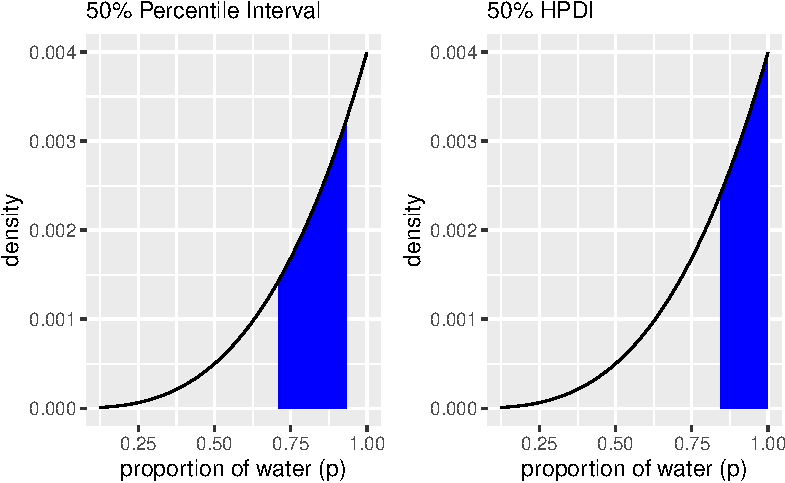
\includegraphics{03-sampling-the-imaginary_files/figure-pdf/figure-3.3-1.pdf}

}

\end{figure}

Again I had to change Kurz's version for the correct result: Instead of
\texttt{tidybayes::hci()} one must use \texttt{tidybayes::hdci()} for
the right hand plot.

Comparing the two panels of the plot you can see that in contrast to the
50\% HPDI the 50\% of PI does not include the highest probability value.

\hypertarget{dots-and-the-pipe}{%
\paragraph{Dots and the Pipe}\label{dots-and-the-pipe}}

\begin{quote}
In the geom\_area() line for the HPDI plot, did you notice how we
replaced \texttt{data\ =\ samples\_skewed\_b} with \texttt{data\ =\ .}?
When using the pipe (i.e., \texttt{\%\textgreater{}\%}), you can use the
\texttt{.} as a placeholder for the original data object. It's an odd
and handy trick to know about.
\end{quote}

(We could have made this change in both parts (p1 and p2) of the graph.
The only condition is that you have used the full name of the data frame
allready in the same piped statement.)

Learn more of the
\href{https://magrittr.tidyverse.org/reference/pipe.html}{pipe function
\%\textgreater\% of the \{\textbf{magrittr}\} package} and about the
\href{https://stat.ethz.ch/R-manual/R-devel/library/base/html/pipeOp.html}{base
R native forward pipe operator}.

The native pipe is available starting with R 4.1.0. It is constructed
with \texttt{\textbar{}} followed by \texttt{\textgreater{}} resulting
in the symbol \texttt{\textbar{}\textgreater{}} to differentiate it from
the \{\textbf{magrittr}\} pipe (\%\textgreater\%). To understand the
details of the differences of \texttt{\%\textgreater{}\%} and the native
R pipe \texttt{\textbar{}\textgreater{}} read this elaborated
\href{https://ivelasq.rbind.io/blog/understanding-the-r-pipe/index.html}{blog
article by Isabella Velásquez}, an employee of
\href{https://posit.co/}{Posit} (formerly RStudio).

\hypertarget{difference-between-pi-and-hpdi}{%
\paragraph{Difference between PI and
HPDI}\label{difference-between-pi-and-hpdi}}

PI and HPDI are only very different if you have a very skewed
distribution. Otherwise they are pretty similar. Let's check this
assertion:

\begin{tcolorbox}[enhanced jigsaw, colframe=quarto-callout-note-color-frame, colback=white, toprule=.15mm, breakable, arc=.35mm, bottomtitle=1mm, colbacktitle=quarto-callout-note-color!10!white, toptitle=1mm, titlerule=0mm, title=\textcolor{quarto-callout-note-color}{\faInfo}\hspace{0.5em}{Note}, leftrule=.75mm, opacityback=0, rightrule=.15mm, opacitybacktitle=0.6, bottomrule=.15mm, left=2mm, coltitle=black]

In this file we have named the variables in the version of the data
frame of 6\texttt{W} with 9 trials different than the variables of the
version of 3\texttt{W} with 3 trials. Therefore we do not need
(re)calculate (= update) the simulation as in Kurz's version.

Furthermore besides \texttt{tidybayes::mean\_qi()} I will use
\texttt{tidybayes::mean\_hdi()} and \texttt{tidybayes::mean\_hdci()}.

\end{tcolorbox}

Try out my own variable names:

\begin{enumerate}
\def\labelenumi{\alph{enumi})}
\tightlist
\item
  Results rounded
\end{enumerate}

\begin{Shaded}
\begin{Highlighting}[]
\InformationTok{\textasciigrave{}\textasciigrave{}\textasciigrave{}\{r\}}
\CommentTok{\#| label: intervals{-}6{-}9{-}not{-}skewed{-}rounded}

\FunctionTok{bind\_rows}\NormalTok{(tidybayes}\SpecialCharTok{::}\FunctionTok{mean\_hdci}\NormalTok{(samples\_b}\SpecialCharTok{$}\NormalTok{samples\_b, }\AttributeTok{.width =} \FunctionTok{c}\NormalTok{(.}\DecValTok{8}\NormalTok{, .}\DecValTok{95}\NormalTok{)),}
\NormalTok{          tidybayes}\SpecialCharTok{::}\FunctionTok{mean\_hdi}\NormalTok{(samples\_b}\SpecialCharTok{$}\NormalTok{samples\_b, }\AttributeTok{.width =} \FunctionTok{c}\NormalTok{(.}\DecValTok{8}\NormalTok{, .}\DecValTok{95}\NormalTok{)),}
\NormalTok{          tidybayes}\SpecialCharTok{::}\FunctionTok{mean\_qi}\NormalTok{(samples\_b}\SpecialCharTok{$}\NormalTok{samples\_b,  }\AttributeTok{.width =} \FunctionTok{c}\NormalTok{(.}\DecValTok{8}\NormalTok{, .}\DecValTok{95}\NormalTok{))) }\SpecialCharTok{\%\textgreater{}\%} 
  \FunctionTok{select}\NormalTok{(.width, .interval, ymin}\SpecialCharTok{:}\NormalTok{ymax) }\SpecialCharTok{\%\textgreater{}\%} 
  \FunctionTok{arrange}\NormalTok{(.width) }\SpecialCharTok{\%\textgreater{}\%} 
  \FunctionTok{mutate\_if}\NormalTok{(is.double, round, }\AttributeTok{digits =} \DecValTok{2}\NormalTok{)}
\InformationTok{\textasciigrave{}\textasciigrave{}\textasciigrave{}}
\end{Highlighting}
\end{Shaded}

\begin{verbatim}
#>   .width .interval ymin ymax
#> 1   0.80      hdci 0.48 0.84
#> 2   0.80       hdi 0.48 0.84
#> 3   0.80        qi 0.45 0.81
#> 4   0.95      hdci 0.37 0.90
#> 5   0.95       hdi 0.37 0.90
#> 6   0.95        qi 0.35 0.88
\end{verbatim}

Sampling from a somewhat Gaussian distribution shows that there are
absolut no differences between \texttt{tidybayes::mean\_hdci()} and
\texttt{tidybayes::mean\_hdi()}.

There are two differences to Kurz's version: 1. \texttt{ymin} of 0.80
\texttt{hdi} is in my version 0.48 and not 0.49. 2. \texttt{ymax} of
0.95 \texttt{hdi} is in my version 0.90 and not 0.89.

I believe that this (very small) differences are rounding errors. But
not rounding errors in the result values but during the complex
\texttt{hdi} calculations as the following not rounded display of values
demonstrate:

\begin{enumerate}
\def\labelenumi{\alph{enumi})}
\setcounter{enumi}{1}
\tightlist
\item
  Results not rounded
\end{enumerate}

\begin{Shaded}
\begin{Highlighting}[]
\InformationTok{\textasciigrave{}\textasciigrave{}\textasciigrave{}\{r\}}
\CommentTok{\#| label: intervals{-}6{-}9{-}not{-}skewed{-}not{-}rounded}

\FunctionTok{bind\_rows}\NormalTok{(tidybayes}\SpecialCharTok{::}\FunctionTok{mean\_hdci}\NormalTok{(samples\_b}\SpecialCharTok{$}\NormalTok{samples\_b, }\AttributeTok{.width =} \FunctionTok{c}\NormalTok{(.}\DecValTok{8}\NormalTok{, .}\DecValTok{95}\NormalTok{)),}
\NormalTok{          tidybayes}\SpecialCharTok{::}\FunctionTok{mean\_hdi}\NormalTok{(samples\_b}\SpecialCharTok{$}\NormalTok{samples\_b, }\AttributeTok{.width =} \FunctionTok{c}\NormalTok{(.}\DecValTok{8}\NormalTok{, .}\DecValTok{95}\NormalTok{)),}
\NormalTok{          tidybayes}\SpecialCharTok{::}\FunctionTok{mean\_qi}\NormalTok{(samples\_b}\SpecialCharTok{$}\NormalTok{samples\_b,  }\AttributeTok{.width =} \FunctionTok{c}\NormalTok{(.}\DecValTok{8}\NormalTok{, .}\DecValTok{95}\NormalTok{))) }\SpecialCharTok{\%\textgreater{}\%} 
  \FunctionTok{select}\NormalTok{(.width, .interval, ymin}\SpecialCharTok{:}\NormalTok{ymax) }\SpecialCharTok{\%\textgreater{}\%} 
  \FunctionTok{arrange}\NormalTok{(.width)}
\InformationTok{\textasciigrave{}\textasciigrave{}\textasciigrave{}}
\end{Highlighting}
\end{Shaded}

\begin{verbatim}
#>   .width .interval      ymin      ymax
#> 1   0.80      hdci 0.4814815 0.8398398
#> 2   0.80       hdi 0.4814815 0.8398398
#> 3   0.80        qi 0.4514515 0.8148148
#> 4   0.95      hdci 0.3723724 0.8958959
#> 5   0.95       hdi 0.3723724 0.8958959
#> 6   0.95        qi 0.3493493 0.8788789
\end{verbatim}

But these small differences are not important. In McElreath words:
\textgreater{} Remember, we're not launching rockets or calibrating atom
smashers, so fetishizing precision to the 5th decimal place will not
improve your science.

The same is true of the small differences between \texttt{qi} and
\texttt{hdi}. They difference is only 2 resp. 3 percent.

\begin{Shaded}
\begin{Highlighting}[]
\InformationTok{\textasciigrave{}\textasciigrave{}\textasciigrave{}\{r\}}
\CommentTok{\#| label: intervals{-}3{-}9{-}skewed{-}version}

\FunctionTok{bind\_rows}\NormalTok{(tidybayes}\SpecialCharTok{::}\FunctionTok{mean\_hdci}\NormalTok{(samples\_skewed\_b}\SpecialCharTok{$}\NormalTok{p\_skewed\_b, }\AttributeTok{.width =} \FunctionTok{c}\NormalTok{(.}\DecValTok{8}\NormalTok{, .}\DecValTok{95}\NormalTok{)),}
\NormalTok{          tidybayes}\SpecialCharTok{::}\FunctionTok{mean\_qi}\NormalTok{(samples\_skewed\_b}\SpecialCharTok{$}\NormalTok{p\_skewed\_b,  }\AttributeTok{.width =} \FunctionTok{c}\NormalTok{(.}\DecValTok{8}\NormalTok{, .}\DecValTok{95}\NormalTok{))) }\SpecialCharTok{\%\textgreater{}\%} 
  \FunctionTok{select}\NormalTok{(.width, .interval, ymin}\SpecialCharTok{:}\NormalTok{ymax) }\SpecialCharTok{\%\textgreater{}\%} 
  \FunctionTok{arrange}\NormalTok{(.width) }\SpecialCharTok{\%\textgreater{}\%} 
  \FunctionTok{mutate\_if}\NormalTok{(is.double, round, }\AttributeTok{digits =} \DecValTok{2}\NormalTok{)}
\InformationTok{\textasciigrave{}\textasciigrave{}\textasciigrave{}}
\end{Highlighting}
\end{Shaded}

\begin{verbatim}
#>   .width .interval ymin ymax
#> 1   0.80      hdci 0.67 1.00
#> 2   0.80        qi 0.57 0.97
#> 3   0.95      hdci 0.48 1.00
#> 4   0.95        qi 0.40 0.99
\end{verbatim}

The skewed version shows bigger differences of 10\% resp. 8\% between
\texttt{mean\_hdci()} and \texttt{mean\_qi()}. (This calculation is
missing in Kurz's version.)

Because of the disadvantages of HPDI (more computationally intensive,
greater simulation variance and harder to understand) we'll primarily
stick to the PI-based intervals.

\hypertarget{point-estimates}{%
\subsection{Point Estimates}\label{point-estimates}}

\hypertarget{original-13}{%
\subsubsection{Original}\label{original-13}}

\begin{quote}
The third and final common summary task for the posterior is to produce
point estimates of some kind. Given the entire posterior distribution,
what value should you report? This seems like an innocent question, but
it is difficult to answer. \textbf{The Bayesian parameter estimate is
precisely the entire posterior distribution, which is not a single
number, but instead a function that maps each unique parameter value
onto a plausibility value.} So really the most important thing to note
is that you don't have to choose a point estimate. It's hardly ever
necessary and often harmful. It discards information. (emphasis is mine,
pb)
\end{quote}

But if you must do it \ldots{} we will take again the globe tossing
experiment in which we observe 3 waters out of 3 tosses, e.g.~the very
skewed distribution.

\hypertarget{calcualte-map}{%
\paragraph{Calcualte MAP}\label{calcualte-map}}

\begin{quote}
First, it is very common for scientists to report the parameter value
with highest posterior probability, a \emph{maximum a posteriori} (MAP)
estimate.
\end{quote}

\begin{Shaded}
\begin{Highlighting}[]
\InformationTok{\textasciigrave{}\textasciigrave{}\textasciigrave{}\{r\}}
\CommentTok{\#| label: calculate{-}skewed{-}MAP{-}grid{-}a}

\DocumentationTok{\#\#\# actually the grid is not skewed. I should change the names accordingly.}

\DocumentationTok{\#\# R code 3.14}
\NormalTok{p\_grid\_skewed\_a[}\FunctionTok{which.max}\NormalTok{(posterior\_skewed\_a)]}
\InformationTok{\textasciigrave{}\textasciigrave{}\textasciigrave{}}
\end{Highlighting}
\end{Shaded}

\begin{verbatim}
#> [1] 1
\end{verbatim}

Or if you instead have samples from the posterior, you can still
approximate the same point:

\begin{Shaded}
\begin{Highlighting}[]
\InformationTok{\textasciigrave{}\textasciigrave{}\textasciigrave{}\{r\}}
\CommentTok{\#| label: calculate{-}skewed{-}MAP{-}samples{-}a}

\DocumentationTok{\#\# R code 3.15}
\NormalTok{rethinking}\SpecialCharTok{::}\FunctionTok{chainmode}\NormalTok{(samples\_skewed\_a, }\AttributeTok{adj =} \FloatTok{0.01}\NormalTok{)}
\InformationTok{\textasciigrave{}\textasciigrave{}\textasciigrave{}}
\end{Highlighting}
\end{Shaded}

\begin{verbatim}
#> [1] 0.9938226
\end{verbatim}

\hypertarget{calculate-measures-of-central-tendency}{%
\paragraph{Calculate measures of central
tendency}\label{calculate-measures-of-central-tendency}}

But why is the MAP, the mode, so interesting? Why not report the
posterior mean or median?

\begin{codelisting}

\caption{Posterior mean and median of the skewed distribution (all three
draws are \texttt{W})}

\hypertarget{lst-mean-median-skewed-samples}{%
\label{lst-mean-median-skewed-samples}}%
\begin{Shaded}
\begin{Highlighting}[]
\InformationTok{\textasciigrave{}\textasciigrave{}\textasciigrave{}\{r\}}
\CommentTok{\#| label: mean{-}median{-}skewed{-}samples{-}a}
\CommentTok{\#| attr{-}source: \textquotesingle{}\#lst{-}mean{-}median{-}skewed{-}samples lst{-}cap="Posterior mean and median of the skewed distribution (all three draws are \textasciigrave{}W\textasciigrave{})"\textquotesingle{}}

\DocumentationTok{\#\# R code 3.16}
\FunctionTok{mean}\NormalTok{(samples\_skewed\_a)}
\FunctionTok{median}\NormalTok{(samples\_skewed\_a)}
\InformationTok{\textasciigrave{}\textasciigrave{}\textasciigrave{}}
\end{Highlighting}
\end{Shaded}

\end{codelisting}

\begin{verbatim}
#> [1] 0.8027632
#> [1] 0.8428428
\end{verbatim}

\hypertarget{plot-postponend}{%
\paragraph{Plot postponend}\label{plot-postponend}}

The graphical representation as shown in Figure 3.4 will be calculated
in the tidyverse version of this section. See:
Picture~\ref{fig-minimum-loss-b} for the left panel and
Picture~\ref{fig-minimum-loss2-b} for the right panel of Figure 3.4.

\begin{quote}
These are also point estimates, and they also summarize the posterior.
But all three---the mode (MAP), mean, and median---are different in this
case. How can we choose?
\end{quote}

\hypertarget{loss-function}{%
\paragraph{Loss function}\label{loss-function}}

One principled way to go beyond using the entire posterior as the
estimate is to choose a \textbf{LOSS FUNCTION}. A loss function is a
rule that tells you the cost associated with using any particular point
estimate. While statisticians and game theorists have long been
interested in loss functions, and how Bayesian inference supports them,
scientists hardly ever use them explicitly. The key insight is that
\emph{different loss functions imply different point estimates}.

\begin{quote}
Calculating expected loss for any given decision means using the
posterior to average over our uncertainty in the true value. Of course
we don't know the true value, in most cases. But if we are going to use
our model's information about the parameter, that means using the entire
posterior distribution. So suppose we decide \(p = 0.5\) will be our
decision. Then the expected loss will be:
\end{quote}

\begin{Shaded}
\begin{Highlighting}[]
\InformationTok{\textasciigrave{}\textasciigrave{}\textasciigrave{}\{r\}}
\CommentTok{\#| label: loss{-}expected{-}0.5{-}a}

\DocumentationTok{\#\# R code 3.17}
\FunctionTok{sum}\NormalTok{(posterior\_skewed\_a }\SpecialCharTok{*} \FunctionTok{abs}\NormalTok{(}\FloatTok{0.5} \SpecialCharTok{{-}}\NormalTok{ p\_grid\_skewed\_a))}
\InformationTok{\textasciigrave{}\textasciigrave{}\textasciigrave{}}
\end{Highlighting}
\end{Shaded}

\begin{verbatim}
#> [1] 0.3128752
\end{verbatim}

\begin{quote}
All the code above does is compute the weighted average loss, where each
loss is weighted by its corresponding posterior probability. There's a
trick for repeating this calculation for every possible decision, using
the function sapply.
\end{quote}

\begin{Shaded}
\begin{Highlighting}[]
\InformationTok{\textasciigrave{}\textasciigrave{}\textasciigrave{}\{r\}}
\CommentTok{\#| label: loss{-}function{-}a}

\DocumentationTok{\#\# R code 3.18}
\NormalTok{loss\_a }\OtherTok{\textless{}{-}} \FunctionTok{sapply}\NormalTok{(p\_grid\_skewed\_a, }\ControlFlowTok{function}\NormalTok{(d) }\FunctionTok{sum}\NormalTok{(posterior\_skewed\_a }\SpecialCharTok{*} \FunctionTok{abs}\NormalTok{(d }\SpecialCharTok{{-}}\NormalTok{ p\_grid\_skewed\_a)))}
\FunctionTok{head}\NormalTok{(loss\_a)}
\InformationTok{\textasciigrave{}\textasciigrave{}\textasciigrave{}}
\end{Highlighting}
\end{Shaded}

\begin{verbatim}
#> [1] 0.8004001 0.7993991 0.7983981 0.7973971 0.7963961 0.7953951
\end{verbatim}

\begin{quote}
Now the symbol \texttt{loss\_a} contains a list of loss values, one for
each possible decision, corresponding the values in
\texttt{p\_grid\_skewed\_a}. From here, it's easy to find the parameter
value that minimizes the loss:
\end{quote}

\begin{Shaded}
\begin{Highlighting}[]
\InformationTok{\textasciigrave{}\textasciigrave{}\textasciigrave{}\{r\}}
\CommentTok{\#| label: minimize{-}loss{-}a}

\DocumentationTok{\#\# R code 3.19}
\NormalTok{p\_grid\_skewed\_a[}\FunctionTok{which.min}\NormalTok{(loss\_a)]}
\InformationTok{\textasciigrave{}\textasciigrave{}\textasciigrave{}}
\end{Highlighting}
\end{Shaded}

\begin{verbatim}
#> [1] 0.8408408
\end{verbatim}

\begin{quote}
And this is actually the posterior median, the parameter value that
splits the posterior density such that half of the mass is above it and
half below it.
\end{quote}

We have already calculated the posterior median in
Listing~\ref{lst-mean-median-skewed-samples}. Because of sampling
variation it is not identical but pretty close (0.8428428
vs.~0.8408408).

\textbf{Learnings}:

\begin{quote}
In order to decide upon a point estimate, a single-value summary of the
posterior distribution, we need to pick a loss function. Different loss
functions nominate different point estimates. The two most common
examples are the absolute loss as above, which leads to the median as
the point estimate, and the quadratic loss \((d - p)^{2}\), which leads
to the posterior mean \texttt{(mean(samples))} as the point estimate.
\end{quote}

\begin{quote}
When the posterior distribution is symmetrical and normal-looking, then
the median and mean converge to the same point, which relaxes some
anxiety we might have about choosing a loss function. For the original
globe tossing data (6 waters in 9 tosses), for example, the mean and
median are barely different.
\end{quote}

\textbf{Comparison of mean \& median} with globe tossing data (6 waters
in 9 tosses) versus (3 waters in 3 tosses):

6/9: Mean = 0.6400664 Median = 0.6486486 3/3: Mean = 0.8027632 Median =
0.8428428

\begin{tcolorbox}[enhanced jigsaw, colframe=quarto-callout-important-color-frame, colback=white, toprule=.15mm, breakable, arc=.35mm, bottomtitle=1mm, colbacktitle=quarto-callout-important-color!10!white, toptitle=1mm, titlerule=0mm, title=\textcolor{quarto-callout-important-color}{\faExclamation}\hspace{0.5em}{Important}, leftrule=.75mm, opacityback=0, rightrule=.15mm, opacitybacktitle=0.6, bottomrule=.15mm, left=2mm, coltitle=black]

Instead of deciding what parameter to report for summarizing the
posterior distribution it is usually better to communicate as much as
you can about the posterior distribution, as well as the data and the
model itself, so that others can build upon your work.

This advice is also valid if you just want to accept or not to accept an
hypothesis. Because the challenge then is to say what the relevant costs
and benefits would be, in terms of the knowledge gained or lost.

\end{tcolorbox}

\hypertarget{tidyverse-13}{%
\subsubsection{Tidyverse}\label{tidyverse-13}}

\hypertarget{calculate-map}{%
\paragraph{Calculate MAP}\label{calculate-map}}

To get the MAP of the skewed version (three tosses with thre \texttt{W})
we have to \texttt{arrange()} our \texttt{d\_b} tibble in descending
order by posterior. Then we will see the corresponding p\_grid\_b value
for its MAP estimate.

\begin{Shaded}
\begin{Highlighting}[]
\InformationTok{\textasciigrave{}\textasciigrave{}\textasciigrave{}\{r\}}
\CommentTok{\#| label: calculate{-}skewed{-}MAP{-}grid{-}b}

\NormalTok{samples\_skewed\_b }\SpecialCharTok{\%\textgreater{}\%} 
  \FunctionTok{arrange}\NormalTok{(}\FunctionTok{desc}\NormalTok{(posterior\_skewed\_b))}
\InformationTok{\textasciigrave{}\textasciigrave{}\textasciigrave{}}
\end{Highlighting}
\end{Shaded}

\begin{verbatim}
#> # A tibble: 10,000 x 6
#>    p_skewed_b prior_skewed_b likelihood_b posterior_b likelihood_skewed_b
#>         <dbl>          <dbl>        <dbl>       <dbl>               <dbl>
#>  1          1              1            0           0                   1
#>  2          1              1            0           0                   1
#>  3          1              1            0           0                   1
#>  4          1              1            0           0                   1
#>  5          1              1            0           0                   1
#>  6          1              1            0           0                   1
#>  7          1              1            0           0                   1
#>  8          1              1            0           0                   1
#>  9          1              1            0           0                   1
#> 10          1              1            0           0                   1
#> # i 9,990 more rows
#> # i 1 more variable: posterior_skewed_b <dbl>
\end{verbatim}

To emphasize it, we can use slice() to select the top row. The MAP value
is the column \texttt{posterior\_skewed\_b}.

\begin{Shaded}
\begin{Highlighting}[]
\InformationTok{\textasciigrave{}\textasciigrave{}\textasciigrave{}\{r\}}
\CommentTok{\#| label: calculate{-}skewed{-}MAP{-}grid2{-}b}

\NormalTok{samples\_skewed\_b }\SpecialCharTok{\%\textgreater{}\%} 
  \FunctionTok{arrange}\NormalTok{(}\FunctionTok{desc}\NormalTok{(posterior\_skewed\_b)) }\SpecialCharTok{|\textgreater{}} 
  \FunctionTok{slice}\NormalTok{(}\DecValTok{1}\NormalTok{)}
\InformationTok{\textasciigrave{}\textasciigrave{}\textasciigrave{}}
\end{Highlighting}
\end{Shaded}

\begin{verbatim}
#> # A tibble: 1 x 6
#>   p_skewed_b prior_skewed_b likelihood_b posterior_b likelihood_skewed_b
#>        <dbl>          <dbl>        <dbl>       <dbl>               <dbl>
#> 1          1              1            0           0                   1
#> # i 1 more variable: posterior_skewed_b <dbl>
\end{verbatim}

\hypertarget{calculate-measures-of-central-tendency-1}{%
\paragraph{Calculate measures of central
tendency}\label{calculate-measures-of-central-tendency-1}}

We can get the mode with \texttt{mode\_hdci()} or \texttt{mode\_qi()}

\begin{Shaded}
\begin{Highlighting}[]
\InformationTok{\textasciigrave{}\textasciigrave{}\textasciigrave{}\{r\}}
\CommentTok{\#| label: tidybayes{-}mode{-}qi{-}and{-}hdci}

\NormalTok{samples\_skewed\_b }\SpecialCharTok{\%\textgreater{}\%}\NormalTok{ tidybayes}\SpecialCharTok{::}\FunctionTok{mode\_qi}\NormalTok{(p\_skewed\_b)}
\NormalTok{samples\_skewed\_b }\SpecialCharTok{\%\textgreater{}\%}\NormalTok{ tidybayes}\SpecialCharTok{::}\FunctionTok{mode\_hdci}\NormalTok{(p\_skewed\_b)}
\InformationTok{\textasciigrave{}\textasciigrave{}\textasciigrave{}}
\end{Highlighting}
\end{Shaded}

\begin{verbatim}
#> # A tibble: 1 x 6
#>   p_skewed_b .lower .upper .width .point .interval
#>        <dbl>  <dbl>  <dbl>  <dbl> <chr>  <chr>    
#> 1       1.00  0.399  0.994   0.95 mode   qi       
#> # A tibble: 1 x 6
#>   p_skewed_b .lower .upper .width .point .interval
#>        <dbl>  <dbl>  <dbl>  <dbl> <chr>  <chr>    
#> 1       1.00  0.475      1   0.95 mode   hdci
\end{verbatim}

Those returned a lot of output in addition to the mode. If all you want
is the mode itself, you can just use \texttt{tidybayes::Mode()}.

\begin{Shaded}
\begin{Highlighting}[]
\InformationTok{\textasciigrave{}\textasciigrave{}\textasciigrave{}\{r\}}
\CommentTok{\#| label: tidybayes{-}mode}

\NormalTok{tidybayes}\SpecialCharTok{::}\FunctionTok{Mode}\NormalTok{(samples\_skewed\_b}\SpecialCharTok{$}\NormalTok{p\_skewed\_b)}
\InformationTok{\textasciigrave{}\textasciigrave{}\textasciigrave{}}
\end{Highlighting}
\end{Shaded}

\begin{verbatim}
#> [1] 0.9995616
\end{verbatim}

Medians and means are typical measures of central tendency, too.

\begin{Shaded}
\begin{Highlighting}[]
\InformationTok{\textasciigrave{}\textasciigrave{}\textasciigrave{}\{r\}}
\CommentTok{\#| label: tidybayes{-}mean{-}and{-}median}

\NormalTok{samples\_skewed\_b }\SpecialCharTok{\%\textgreater{}\%} 
  \FunctionTok{summarise}\NormalTok{(}\AttributeTok{mean   =} \FunctionTok{mean}\NormalTok{(p\_skewed\_b),}
            \AttributeTok{median =} \FunctionTok{median}\NormalTok{(p\_skewed\_b))}
\InformationTok{\textasciigrave{}\textasciigrave{}\textasciigrave{}}
\end{Highlighting}
\end{Shaded}

\begin{verbatim}
#> # A tibble: 1 x 2
#>    mean median
#>   <dbl>  <dbl>
#> 1 0.803  0.843
\end{verbatim}

\hypertarget{plot-left-panel-of-figure-3.4}{%
\paragraph{Plot left panel of figure
3.4}\label{plot-left-panel-of-figure-3.4}}

\begin{enumerate}
\def\labelenumi{\arabic{enumi}.}
\tightlist
\item
  Bundle the three types of estimates into a tibble
\end{enumerate}

\begin{Shaded}
\begin{Highlighting}[]
\InformationTok{\textasciigrave{}\textasciigrave{}\textasciigrave{}\{r\}}
\CommentTok{\#| label: bundle{-}skewed{-}point{-}estimates}

\NormalTok{(}
\NormalTok{  point\_estimates\_b }\OtherTok{\textless{}{-}}
  \FunctionTok{bind\_rows}\NormalTok{(samples\_skewed\_b }\SpecialCharTok{\%\textgreater{}\%}\NormalTok{ tidybayes}\SpecialCharTok{::}\FunctionTok{mean\_qi}\NormalTok{(p\_skewed\_b),}
\NormalTok{            samples\_skewed\_b }\SpecialCharTok{\%\textgreater{}\%}\NormalTok{ tidybayes}\SpecialCharTok{::}\FunctionTok{median\_qi}\NormalTok{(p\_skewed\_b),}
\NormalTok{            samples\_skewed\_b }\SpecialCharTok{\%\textgreater{}\%}\NormalTok{ tidybayes}\SpecialCharTok{::}\FunctionTok{mode\_qi}\NormalTok{(p\_skewed\_b)) }\SpecialCharTok{\%\textgreater{}\%} 
  \FunctionTok{select}\NormalTok{(p\_skewed\_b, .point) }\SpecialCharTok{\%\textgreater{}\%} 
  \CommentTok{\# these last two columns will help us annotate  }
  \FunctionTok{mutate}\NormalTok{(}\AttributeTok{x =}\NormalTok{ p\_skewed\_b }\SpecialCharTok{+} \FunctionTok{c}\NormalTok{(}\SpecialCharTok{{-}}\NormalTok{.}\DecValTok{03}\NormalTok{, .}\DecValTok{03}\NormalTok{, }\SpecialCharTok{{-}}\NormalTok{.}\DecValTok{03}\NormalTok{),}
         \AttributeTok{y =} \FunctionTok{c}\NormalTok{(.}\DecValTok{0005}\NormalTok{, .}\DecValTok{0012}\NormalTok{, .}\DecValTok{002}\NormalTok{))}
\NormalTok{)}
\InformationTok{\textasciigrave{}\textasciigrave{}\textasciigrave{}}
\end{Highlighting}
\end{Shaded}

\begin{verbatim}
#> # A tibble: 3 x 4
#>   p_skewed_b .point     x      y
#>        <dbl> <chr>  <dbl>  <dbl>
#> 1      0.803 mean   0.773 0.0005
#> 2      0.843 median 0.873 0.0012
#> 3      1.00  mode   0.970 0.002
\end{verbatim}

Plotting the results:

\begin{Shaded}
\begin{Highlighting}[]
\InformationTok{\textasciigrave{}\textasciigrave{}\textasciigrave{}\{r\}}
\CommentTok{\#| label: fig{-}skewed{-}point{-}estimates\_b}
\CommentTok{\#| fig{-}cap: "Posterior distribution (blue) after observing 3 water in 3 tosses of the globe. Vertical lines show the locations of the mode, median, and mean. Each point implies a different loss function."}

\NormalTok{samples\_skewed\_b }\SpecialCharTok{\%\textgreater{}\%} 
  \FunctionTok{ggplot}\NormalTok{(}\FunctionTok{aes}\NormalTok{(}\AttributeTok{x =}\NormalTok{ p\_skewed\_b)) }\SpecialCharTok{+}
  \FunctionTok{geom\_area}\NormalTok{(}\FunctionTok{aes}\NormalTok{(}\AttributeTok{y =}\NormalTok{ posterior\_skewed\_b),}
            \AttributeTok{fill =} \StringTok{"deepskyblue"}\NormalTok{) }\SpecialCharTok{+}
  \FunctionTok{geom\_vline}\NormalTok{(}\AttributeTok{xintercept =}\NormalTok{ point\_estimates\_b}\SpecialCharTok{$}\NormalTok{p\_skewed\_b) }\SpecialCharTok{+}
  \FunctionTok{geom\_text}\NormalTok{(}\AttributeTok{data =}\NormalTok{ point\_estimates\_b,}
            \FunctionTok{aes}\NormalTok{(}\AttributeTok{x =}\NormalTok{ x, }\AttributeTok{y =}\NormalTok{ y, }\AttributeTok{label =}\NormalTok{ .point),}
            \AttributeTok{angle =} \DecValTok{90}\NormalTok{) }\SpecialCharTok{+}
  \FunctionTok{labs}\NormalTok{(}\AttributeTok{x =} \StringTok{"proportion of water (p)"}\NormalTok{,}
       \AttributeTok{y =} \StringTok{"density"}\NormalTok{) }\SpecialCharTok{+}
  \FunctionTok{theme}\NormalTok{(}\AttributeTok{panel.grid =} \FunctionTok{element\_blank}\NormalTok{())}
\InformationTok{\textasciigrave{}\textasciigrave{}\textasciigrave{}}
\end{Highlighting}
\end{Shaded}

\begin{figure}[H]

{\centering 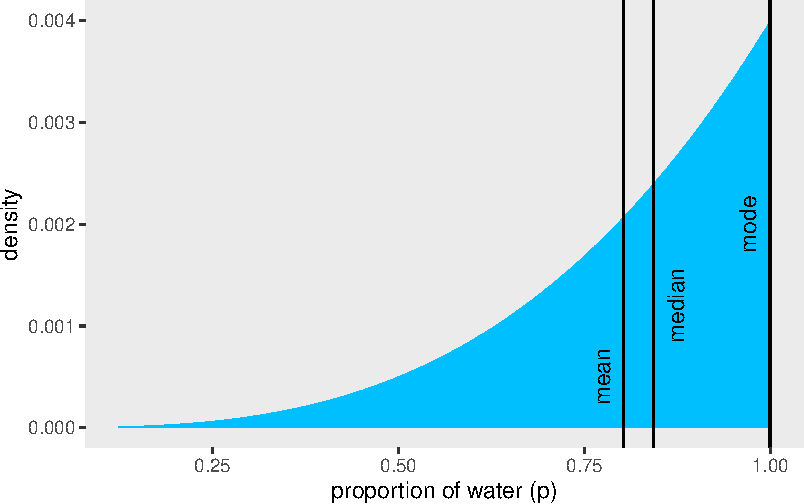
\includegraphics{03-sampling-the-imaginary_files/figure-pdf/fig-skewed-point-estimates_b-1.pdf}

}

\caption{\label{fig-skewed-point-estimates_b}Posterior distribution
(blue) after observing 3 water in 3 tosses of the globe. Vertical lines
show the locations of the mode, median, and mean. Each point implies a
different loss function.}

\end{figure}

In contrast the other distribution with 6 successes by 9 trials
(tosses):

\begin{Shaded}
\begin{Highlighting}[]
\InformationTok{\textasciigrave{}\textasciigrave{}\textasciigrave{}\{r\}}
\CommentTok{\#| label: fig{-}sym{-}point{-}estimates\_b}
\CommentTok{\#| fig{-}cap: "Point estimates in the almost symmetrical distribution of 6 successes (\textasciigrave{}W\textasciigrave{}) in 9 tosses."}

\NormalTok{(}
\NormalTok{    point\_estimates\_b }\OtherTok{\textless{}{-}}
      \FunctionTok{bind\_rows}\NormalTok{(samples\_b }\SpecialCharTok{\%\textgreater{}\%}\NormalTok{ tidybayes}\SpecialCharTok{::}\FunctionTok{mean\_qi}\NormalTok{(samples\_b),}
\NormalTok{                samples\_b }\SpecialCharTok{\%\textgreater{}\%}\NormalTok{ tidybayes}\SpecialCharTok{::}\FunctionTok{median\_qi}\NormalTok{(samples\_b),}
\NormalTok{                samples\_b }\SpecialCharTok{\%\textgreater{}\%}\NormalTok{ tidybayes}\SpecialCharTok{::}\FunctionTok{mode\_qi}\NormalTok{(samples\_b)) }\SpecialCharTok{\%\textgreater{}\%} 
      \FunctionTok{select}\NormalTok{(samples\_b, .point) }\SpecialCharTok{\%\textgreater{}\%} 
      \CommentTok{\# these last two columns will help us annotate  }
      \FunctionTok{mutate}\NormalTok{(}\AttributeTok{x =}\NormalTok{ samples\_b }\SpecialCharTok{+} \FunctionTok{c}\NormalTok{(}\SpecialCharTok{{-}}\NormalTok{.}\DecValTok{03}\NormalTok{, .}\DecValTok{03}\NormalTok{, }\SpecialCharTok{{-}}\NormalTok{.}\DecValTok{03}\NormalTok{),}
             \AttributeTok{y =} \FunctionTok{c}\NormalTok{(.}\DecValTok{0005}\NormalTok{, .}\DecValTok{0012}\NormalTok{, .}\DecValTok{002}\NormalTok{))}
\NormalTok{)}

\NormalTok{samples\_b }\SpecialCharTok{\%\textgreater{}\%} 
  \FunctionTok{ggplot}\NormalTok{(}\FunctionTok{aes}\NormalTok{(}\AttributeTok{x =}\NormalTok{ samples\_b)) }\SpecialCharTok{+}
  \FunctionTok{geom\_area}\NormalTok{(}\FunctionTok{aes}\NormalTok{(}\AttributeTok{y =}\NormalTok{ posterior\_samples\_b),}
            \AttributeTok{fill =} \StringTok{"deepskyblue"}\NormalTok{) }\SpecialCharTok{+}
  \FunctionTok{geom\_vline}\NormalTok{(}\AttributeTok{xintercept =}\NormalTok{ point\_estimates\_b}\SpecialCharTok{$}\NormalTok{samples\_b) }\SpecialCharTok{+}
  \FunctionTok{geom\_text}\NormalTok{(}\AttributeTok{data =}\NormalTok{ point\_estimates\_b,}
            \FunctionTok{aes}\NormalTok{(}\AttributeTok{x =}\NormalTok{ x, }\AttributeTok{y =}\NormalTok{ y, }\AttributeTok{label =}\NormalTok{ .point),}
            \AttributeTok{angle =} \DecValTok{90}\NormalTok{) }\SpecialCharTok{+}
  \FunctionTok{labs}\NormalTok{(}\AttributeTok{x =} \StringTok{"proportion of water (p)"}\NormalTok{,}
       \AttributeTok{y =} \StringTok{"density"}\NormalTok{) }\SpecialCharTok{+}
  \FunctionTok{theme}\NormalTok{(}\AttributeTok{panel.grid =} \FunctionTok{element\_blank}\NormalTok{())}
\InformationTok{\textasciigrave{}\textasciigrave{}\textasciigrave{}}
\end{Highlighting}
\end{Shaded}

\begin{verbatim}
#> # A tibble: 3 x 4
#>   samples_b .point     x      y
#>       <dbl> <chr>  <dbl>  <dbl>
#> 1     0.640 mean   0.610 0.0005
#> 2     0.649 median 0.679 0.0012
#> 3     0.651 mode   0.621 0.002
\end{verbatim}

\begin{figure}[H]

{\centering 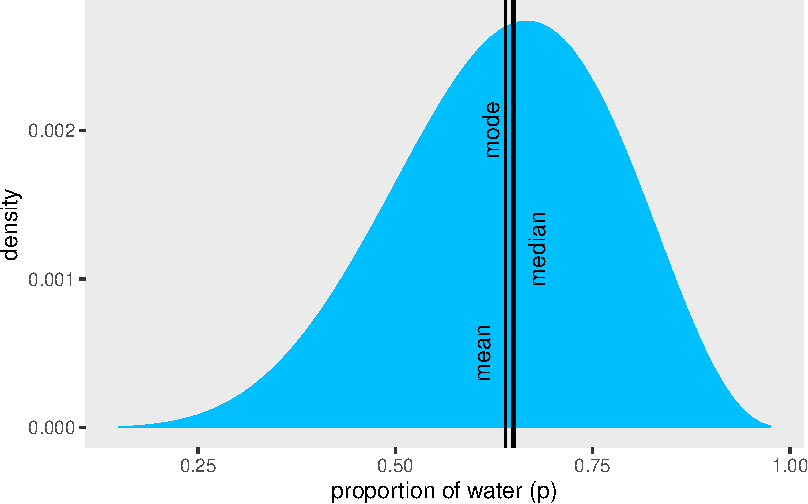
\includegraphics{03-sampling-the-imaginary_files/figure-pdf/fig-sym-point-estimates_b-1.pdf}

}

\caption{\label{fig-sym-point-estimates_b}Point estimates in the almost
symmetrical distribution of 6 successes (\texttt{W}) in 9 tosses.}

\end{figure}

\hypertarget{loss-function-1}{%
\paragraph{Loss function}\label{loss-function-1}}

Let \(p\) be the proportion of the Earth covered by water and \(d\) be
our guess. If McElreath pays us \$100 if we guess exactly right but
subtracts money from the prize proportional to how far off we are, then
our loss is proportional to \(d - p\). If we decide \(d = .5\), we can
compute our expected loss.

\begin{Shaded}
\begin{Highlighting}[]
\InformationTok{\textasciigrave{}\textasciigrave{}\textasciigrave{}\{r\}}
\CommentTok{\#| label: loss{-}epected{-}0.5{-}b}

\NormalTok{d\_skewed\_b }\SpecialCharTok{|\textgreater{}} 
    \FunctionTok{summarise}\NormalTok{(}\StringTok{\textasciigrave{}}\AttributeTok{expected loss}\StringTok{\textasciigrave{}} \OtherTok{=} \FunctionTok{sum}\NormalTok{(posterior\_skewed\_b }\SpecialCharTok{*} \FunctionTok{abs}\NormalTok{(}\FloatTok{0.5} \SpecialCharTok{{-}}\NormalTok{ p\_grid\_b)))}
\InformationTok{\textasciigrave{}\textasciigrave{}\textasciigrave{}}
\end{Highlighting}
\end{Shaded}

\begin{verbatim}
#> # A tibble: 1 x 1
#>   `expected loss`
#>             <dbl>
#> 1           0.313
\end{verbatim}

The \texttt{map()} family of the
\href{https://purrr.tidyverse.org/}{\{\textbf{purrr}\} package} is the
tidyverse alternative to the family of \texttt{apply()} functions from
the base R framework. You can learn more about how to use the
\texttt{map()} family on different places:

\begin{itemize}
\tightlist
\item
  \href{https://purrr.tidyverse.org/reference/map.html}{Purrr
  reference}: Apply a function to each element of a vector
\item
  \href{https://jennybc.github.io/purrr-tutorial/ls01_map-name-position-shortcuts.html}{Purrr
  tutorial}: Introduction to map(): extract elements
\item
  \href{https://data.library.virginia.edu/getting-started-with-the-purrr-package-in-r/}{University
  of Virginia Library}: Getting Started with the purrr Package in R
\end{itemize}

Calculate loss function

\begin{Shaded}
\begin{Highlighting}[]
\InformationTok{\textasciigrave{}\textasciigrave{}\textasciigrave{}\{r\}}
\CommentTok{\#| label: loss{-}function{-}b}

\NormalTok{make\_loss\_b }\OtherTok{\textless{}{-}} \ControlFlowTok{function}\NormalTok{(our\_d) \{}
\NormalTok{  d\_skewed\_b }\SpecialCharTok{\%\textgreater{}\%} 
    \FunctionTok{mutate}\NormalTok{(}\AttributeTok{loss\_b =}\NormalTok{ posterior\_skewed\_b }\SpecialCharTok{*} \FunctionTok{abs}\NormalTok{(our\_d }\SpecialCharTok{{-}}\NormalTok{ p\_grid\_b)) }\SpecialCharTok{\%\textgreater{}\%} 
    \FunctionTok{summarise}\NormalTok{(}\AttributeTok{weighted\_average\_loss\_b =} \FunctionTok{sum}\NormalTok{(loss\_b))}
\NormalTok{\}}

\NormalTok{(}
\NormalTok{  l\_b }\OtherTok{\textless{}{-}}
\NormalTok{  d\_skewed\_b }\SpecialCharTok{\%\textgreater{}\%} 
  \FunctionTok{select}\NormalTok{(p\_grid\_b) }\SpecialCharTok{\%\textgreater{}\%} 
  \FunctionTok{rename}\NormalTok{(}\AttributeTok{decision\_b =}\NormalTok{ p\_grid\_b) }\SpecialCharTok{\%\textgreater{}\%} 
  \FunctionTok{mutate}\NormalTok{(}\AttributeTok{weighted\_average\_loss\_b =}\NormalTok{ purrr}\SpecialCharTok{::}\FunctionTok{map}\NormalTok{(decision\_b, make\_loss\_b)) }\SpecialCharTok{\%\textgreater{}\%} 
  \FunctionTok{unnest}\NormalTok{(weighted\_average\_loss\_b) }
\NormalTok{)}
\InformationTok{\textasciigrave{}\textasciigrave{}\textasciigrave{}}
\end{Highlighting}
\end{Shaded}

\begin{verbatim}
#> # A tibble: 1,000 x 2
#>    decision_b weighted_average_loss_b
#>         <dbl>                   <dbl>
#>  1    0                         0.800
#>  2    0.00100                   0.799
#>  3    0.00200                   0.798
#>  4    0.00300                   0.797
#>  5    0.00400                   0.796
#>  6    0.00501                   0.795
#>  7    0.00601                   0.794
#>  8    0.00701                   0.793
#>  9    0.00801                   0.792
#> 10    0.00901                   0.791
#> # i 990 more rows
\end{verbatim}

Calculate the minimum loss

\begin{Shaded}
\begin{Highlighting}[]
\InformationTok{\textasciigrave{}\textasciigrave{}\textasciigrave{}\{r\}}
\CommentTok{\#| label: minimize{-}loss{-}b}

\CommentTok{\# this will help us find the x and y coordinates for the minimum value}
\NormalTok{(}
\NormalTok{    min\_loss\_b }\OtherTok{\textless{}{-}}
\NormalTok{      l\_b }\SpecialCharTok{\%\textgreater{}\%} 
      \FunctionTok{filter}\NormalTok{(weighted\_average\_loss\_b }\SpecialCharTok{==} \FunctionTok{min}\NormalTok{(weighted\_average\_loss\_b)) }\SpecialCharTok{\%\textgreater{}\%} 
      \FunctionTok{as.numeric}\NormalTok{()}
\NormalTok{)}
\InformationTok{\textasciigrave{}\textasciigrave{}\textasciigrave{}}
\end{Highlighting}
\end{Shaded}

\begin{verbatim}
#> [1] 0.8408408 0.1273465
\end{verbatim}

Now we're ready for the right panel of Figure 3.4.

\begin{Shaded}
\begin{Highlighting}[]
\InformationTok{\textasciigrave{}\textasciigrave{}\textasciigrave{}\{r\}}
\CommentTok{\#| label: fig{-}minimum{-}loss{-}b}
\CommentTok{\#| fig{-}cap: "Expected loss under the rule that loss is proportional to absolute distance of decision (horizontal axis) from the true value. The point marks the value of \textasciigrave{}p\textasciigrave{} that minimizes the expected loss, the posterior median."}

\NormalTok{l\_b }\SpecialCharTok{\%\textgreater{}\%}   
  \FunctionTok{ggplot}\NormalTok{(}\FunctionTok{aes}\NormalTok{(}\AttributeTok{x =}\NormalTok{ decision\_b, }\AttributeTok{y =}\NormalTok{ weighted\_average\_loss\_b)) }\SpecialCharTok{+}
  \FunctionTok{geom\_area}\NormalTok{(}\AttributeTok{fill =} \StringTok{"deepskyblue"}\NormalTok{) }\SpecialCharTok{+}
  \FunctionTok{geom\_vline}\NormalTok{(}\AttributeTok{xintercept =}\NormalTok{ min\_loss\_b[}\DecValTok{1}\NormalTok{], }\AttributeTok{color =} \StringTok{"black"}\NormalTok{, }\AttributeTok{linetype =} \DecValTok{3}\NormalTok{) }\SpecialCharTok{+}
  \FunctionTok{geom\_hline}\NormalTok{(}\AttributeTok{yintercept =}\NormalTok{ min\_loss\_b[}\DecValTok{2}\NormalTok{], }\AttributeTok{color =} \StringTok{"black"}\NormalTok{, }\AttributeTok{linetype =} \DecValTok{3}\NormalTok{) }\SpecialCharTok{+}
  \FunctionTok{ylab}\NormalTok{(}\StringTok{"expected proportional loss"}\NormalTok{) }\SpecialCharTok{+}
  \FunctionTok{theme}\NormalTok{(}\AttributeTok{panel.grid =} \FunctionTok{element\_blank}\NormalTok{())}
\InformationTok{\textasciigrave{}\textasciigrave{}\textasciigrave{}}
\end{Highlighting}
\end{Shaded}

\begin{figure}[H]

{\centering 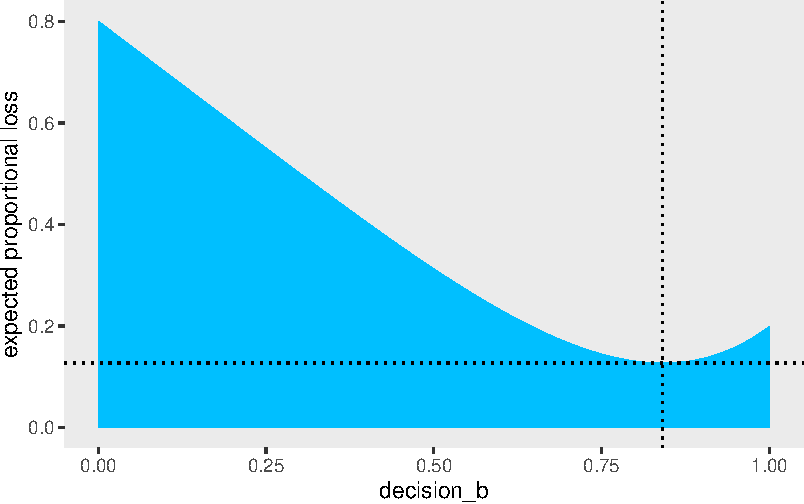
\includegraphics{03-sampling-the-imaginary_files/figure-pdf/fig-minimum-loss-b-1.pdf}

}

\caption{\label{fig-minimum-loss-b}Expected loss under the rule that
loss is proportional to absolute distance of decision (horizontal axis)
from the true value. The point marks the value of \texttt{p} that
minimizes the expected loss, the posterior median.}

\end{figure}

We saved the exact minimum value as \texttt{min\_loss\_b{[}1{]}}, which
is 0.8408408. Within sampling error, this is the posterior median as
depicted by our samples.

\begin{Shaded}
\begin{Highlighting}[]
\InformationTok{\textasciigrave{}\textasciigrave{}\textasciigrave{}\{r\}}
\CommentTok{\#| label: posterior{-}skewed{-}median\_b}

\NormalTok{samples\_skewed\_b }\SpecialCharTok{\%\textgreater{}\%} 
  \FunctionTok{summarise}\NormalTok{(}\AttributeTok{posterior\_median\_b =} \FunctionTok{median}\NormalTok{(p\_skewed\_b))}
\InformationTok{\textasciigrave{}\textasciigrave{}\textasciigrave{}}
\end{Highlighting}
\end{Shaded}

\begin{verbatim}
#> # A tibble: 1 x 1
#>   posterior_median_b
#>                <dbl>
#> 1              0.843
\end{verbatim}

The quadratic loss \((d−p)^{2}\) suggests we should use the mean
instead. Let's investigate.

\begin{Shaded}
\begin{Highlighting}[]
\InformationTok{\textasciigrave{}\textasciigrave{}\textasciigrave{}\{r\}}
\CommentTok{\#| label: fig{-}minimum{-}loss2{-}b}
\CommentTok{\#| fig{-}cap: "Expected loss under the rule that loss is quadratic to the distance of decision (horizontal axis) from the true value. The point marks the value of \textasciigrave{}p\textasciigrave{} that minimizes the expected loss, the posterior mean"}

\CommentTok{\# amend our loss function}

\NormalTok{make\_loss2\_b }\OtherTok{\textless{}{-}} \ControlFlowTok{function}\NormalTok{(our\_d2) \{}
\NormalTok{  d\_skewed\_b }\SpecialCharTok{\%\textgreater{}\%} 
    \FunctionTok{mutate}\NormalTok{(}\AttributeTok{loss2\_b =}\NormalTok{ posterior\_skewed\_b }\SpecialCharTok{*}\NormalTok{ (our\_d2 }\SpecialCharTok{{-}}\NormalTok{ p\_grid\_b)}\SpecialCharTok{\^{}}\DecValTok{2}\NormalTok{) }\SpecialCharTok{\%\textgreater{}\%} 
    \FunctionTok{summarise}\NormalTok{(}\AttributeTok{weighted\_average\_loss2\_b =} \FunctionTok{sum}\NormalTok{(loss2\_b))}
\NormalTok{\}}


\CommentTok{\# remake our \textasciigrave{}l\textasciigrave{} data}
\NormalTok{l2\_b }\OtherTok{\textless{}{-}}
\NormalTok{  d\_skewed\_b }\SpecialCharTok{\%\textgreater{}\%} 
  \FunctionTok{select}\NormalTok{(p\_grid\_b) }\SpecialCharTok{\%\textgreater{}\%} 
  \FunctionTok{rename}\NormalTok{(}\AttributeTok{decision2\_b =}\NormalTok{ p\_grid\_b) }\SpecialCharTok{\%\textgreater{}\%} 
  \FunctionTok{mutate}\NormalTok{(}\AttributeTok{weighted\_average\_loss2\_b =}\NormalTok{ purrr}\SpecialCharTok{::}\FunctionTok{map}\NormalTok{(decision2\_b, make\_loss2\_b)) }\SpecialCharTok{\%\textgreater{}\%} 
  \FunctionTok{unnest}\NormalTok{(weighted\_average\_loss2\_b)}

\CommentTok{\# update to the new minimum loss coordinates}

\NormalTok{(}
\NormalTok{    min\_loss2\_b }\OtherTok{\textless{}{-}}
\NormalTok{      l2\_b }\SpecialCharTok{\%\textgreater{}\%} 
      \FunctionTok{filter}\NormalTok{(weighted\_average\_loss2\_b }\SpecialCharTok{==} \FunctionTok{min}\NormalTok{(weighted\_average\_loss2\_b)) }\SpecialCharTok{\%\textgreater{}\%} 
      \FunctionTok{as.numeric}\NormalTok{()}
\NormalTok{)}

\CommentTok{\# update the plot}
\NormalTok{l2\_b }\SpecialCharTok{\%\textgreater{}\%}   
  \FunctionTok{ggplot}\NormalTok{(}\FunctionTok{aes}\NormalTok{(}\AttributeTok{x =}\NormalTok{ decision2\_b, }\AttributeTok{y =}\NormalTok{ weighted\_average\_loss2\_b)) }\SpecialCharTok{+}
  \FunctionTok{geom\_area}\NormalTok{(}\AttributeTok{fill =} \StringTok{"deepskyblue"}\NormalTok{) }\SpecialCharTok{+}
  \FunctionTok{geom\_vline}\NormalTok{(}\AttributeTok{xintercept =}\NormalTok{ min\_loss2\_b[}\DecValTok{1}\NormalTok{], }\AttributeTok{color =} \StringTok{"black"}\NormalTok{, }\AttributeTok{linetype =} \DecValTok{3}\NormalTok{) }\SpecialCharTok{+}
  \FunctionTok{geom\_hline}\NormalTok{(}\AttributeTok{yintercept =}\NormalTok{ min\_loss2\_b[}\DecValTok{2}\NormalTok{], }\AttributeTok{color =} \StringTok{"black"}\NormalTok{, }\AttributeTok{linetype =} \DecValTok{3}\NormalTok{) }\SpecialCharTok{+}
  \FunctionTok{ylab}\NormalTok{(}\StringTok{"expected proportional loss"}\NormalTok{) }\SpecialCharTok{+}
  \FunctionTok{theme}\NormalTok{(}\AttributeTok{panel.grid =} \FunctionTok{element\_blank}\NormalTok{())}
\InformationTok{\textasciigrave{}\textasciigrave{}\textasciigrave{}}
\end{Highlighting}
\end{Shaded}

\begin{verbatim}
#> [1] 0.80080080 0.02669345
\end{verbatim}

\begin{figure}[H]

{\centering 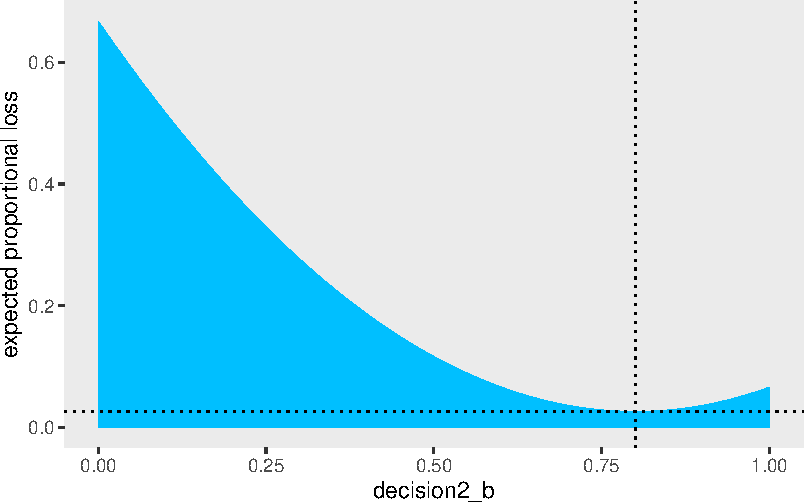
\includegraphics{03-sampling-the-imaginary_files/figure-pdf/fig-minimum-loss2-b-1.pdf}

}

\caption{\label{fig-minimum-loss2-b}Expected loss under the rule that
loss is quadratic to the distance of decision (horizontal axis) from the
true value. The point marks the value of \texttt{p} that minimizes the
expected loss, the posterior mean}

\end{figure}

Based on quadratic loss \((d−p)^{2}\), the exact minimum value is
0.8008008. Within sampling error, this is the posterior mean of our
samples.

\begin{Shaded}
\begin{Highlighting}[]
\InformationTok{\textasciigrave{}\textasciigrave{}\textasciigrave{}\{r\}}
\CommentTok{\#| label: posterior{-}skewed{-}mean\_b}

\NormalTok{samples\_skewed\_b }\SpecialCharTok{\%\textgreater{}\%} 
  \FunctionTok{summarise}\NormalTok{(}\AttributeTok{posterior\_mean\_b =} \FunctionTok{mean}\NormalTok{(p\_skewed\_b))}
\InformationTok{\textasciigrave{}\textasciigrave{}\textasciigrave{}}
\end{Highlighting}
\end{Shaded}

\begin{verbatim}
#> # A tibble: 1 x 1
#>   posterior_mean_b
#>              <dbl>
#> 1            0.803
\end{verbatim}

\hypertarget{sampling-to-simulate-prediction}{%
\section{Sampling to simulate
prediction}\label{sampling-to-simulate-prediction}}

\hypertarget{original-14}{%
\subsection{Original}\label{original-14}}

To generate implied observations from a model is useful for at least
five reasons:

\begin{enumerate}
\def\labelenumi{\arabic{enumi}.}
\tightlist
\item
  \textbf{Model design}: We can sample not only from the posterior, but
  also from the prior. Seeing what the model expects, before the data
  arrive, is the best way to understand the implications of the prior.
  We'll do a lot of this in later chapters, where there will be multiple
  parameters and so their joint implications are not always very clear.
\item
  \textbf{Model checking}: After a model is updated using data, it is
  worth simulating implied observations, to check both whether the fit
  worked correctly and to investigate model behavior.
\item
  \textbf{Software validation}: In order to be sure that our model
  fitting software is working, it helps to simulate observations under a
  known model and then attempt to recover the values of the parameters
  the data were simulated under.
\item
  \textbf{Research design}: If you can simulate observations from your
  hypothesis, then you can evaluate whether the research design can be
  effective. In a narrow sense, this means doing power analysis, but the
  possibilities are much broader.
\item
  \textbf{Forecasting}: Estimates can be used to simulate new
  predictions, for new cases and future observations. These forecasts
  can be useful as applied prediction, but also for model criticism and
  revision.
\end{enumerate}

\hypertarget{dummy-data}{%
\subsubsection{Dummy data}\label{dummy-data}}

\begin{quote}
Now note that these assumptions not only allow us to infer the
plausibility of each possible value of \emph{p}, after observation.
That's what you did in the previous chapter. These assumptions also
allow us to simulate the observations that the model implies. They allow
this, because likelihood functions work in both directions. Given a
realized observation, the likelihood function says how plausible the
observation is. And given only the parameters, the likelihood defines a
distribution of possible observations that we can sample from, to
simulate observation. In this way, Bayesian models are always
\emph{generative}, capable of simulating predictions. Many non-Bayesian
models are also generative, but many are not.

We will call such simulated data \textbf{DUMMY DATA}, to indicate that
it is a stand-in for actual data.
\end{quote}

\hypertarget{probability-of-each-globe-toss}{%
\paragraph{Probability of each globe
toss}\label{probability-of-each-globe-toss}}

\begin{quote}
Suppose \(N = 2\), two tosses of the globe. Then there are only three
possible observations: 0 water, 1 water, 2 water. You can quickly
compute the probability of each, for any given value of \emph{p}. Let's
use \(p = 0.7\), which is just about the true proportion of water on the
Earth:
\end{quote}

\begin{Shaded}
\begin{Highlighting}[]
\InformationTok{\textasciigrave{}\textasciigrave{}\textasciigrave{}\{r\}}
\CommentTok{\#| label: dummy{-}data{-}a}

\DocumentationTok{\#\# R code 3.20}
\FunctionTok{dbinom}\NormalTok{(}\DecValTok{0}\SpecialCharTok{:}\DecValTok{2}\NormalTok{, }\AttributeTok{size =} \DecValTok{2}\NormalTok{, }\AttributeTok{prob =} \FloatTok{0.7}\NormalTok{)}
\InformationTok{\textasciigrave{}\textasciigrave{}\textasciigrave{}}
\end{Highlighting}
\end{Shaded}

\begin{verbatim}
#> [1] 0.09 0.42 0.49
\end{verbatim}

\hypertarget{simulation-of-glob-tosses}{%
\paragraph{Simulation of glob tosses}\label{simulation-of-glob-tosses}}

\begin{quote}
Now we're going to simulate observations, using these probabilities.
This is done by sampling from the distribution just described above. You
could use \texttt{sample()} to do this, but R provides convenient
sampling functions for all the ordinary probability distributions, like
the binomial.
\end{quote}

\begin{Shaded}
\begin{Highlighting}[]
\InformationTok{\textasciigrave{}\textasciigrave{}\textasciigrave{}\{r\}}
\CommentTok{\#| label: simulate{-}1{-}obs{-}a}

\FunctionTok{set.seed}\NormalTok{(}\DecValTok{3}\NormalTok{) }\CommentTok{\# for reproducibility}

\DocumentationTok{\#\# R code 3.21}
\FunctionTok{rbinom}\NormalTok{(}\DecValTok{1}\NormalTok{, }\AttributeTok{size =} \DecValTok{2}\NormalTok{, }\AttributeTok{prob =} \FloatTok{0.7}\NormalTok{)}
\InformationTok{\textasciigrave{}\textasciigrave{}\textasciigrave{}}
\end{Highlighting}
\end{Shaded}

\begin{verbatim}
#> [1] 2
\end{verbatim}

(As the outcome results from a random process the above value differs
from the SR2 version. But with \texttt{set.seed(3)}` you will get the
same value of \(2\).)

\begin{quote}
That \(1\) means ``2 water in 2 tosses.'' The ``\texttt{r}'' in
\texttt{rbinom} stands for ``random.'' It can also generate more than
one simulation at a time. A set of 10 simulations can be made by:
\end{quote}

\begin{Shaded}
\begin{Highlighting}[]
\InformationTok{\textasciigrave{}\textasciigrave{}\textasciigrave{}\{r\}}
\CommentTok{\#| label: simulate{-}10{-}obs{-}a}

\FunctionTok{set.seed}\NormalTok{(}\DecValTok{3}\NormalTok{)}
\DocumentationTok{\#\# R code 3.22}
\FunctionTok{rbinom}\NormalTok{(}\DecValTok{10}\NormalTok{, }\AttributeTok{size =} \DecValTok{2}\NormalTok{, }\AttributeTok{prob =} \FloatTok{0.7}\NormalTok{)}
\InformationTok{\textasciigrave{}\textasciigrave{}\textasciigrave{}}
\end{Highlighting}
\end{Shaded}

\begin{verbatim}
#>  [1] 2 1 2 2 1 1 2 2 1 1
\end{verbatim}

\begin{quote}
Let's generate 100,000 dummy observations, just to verify that each
value (0, 1, or 2) appears in proportion to its likelihood:
\end{quote}

\begin{Shaded}
\begin{Highlighting}[]
\InformationTok{\textasciigrave{}\textasciigrave{}\textasciigrave{}\{r\}}
\CommentTok{\#| label: simulate{-}2e5{-}obs{-}a}

\FunctionTok{set.seed}\NormalTok{(}\DecValTok{3}\NormalTok{)}
\DocumentationTok{\#\# R code 3.23}
\NormalTok{dummy\_w\_a }\OtherTok{\textless{}{-}} \FunctionTok{rbinom}\NormalTok{(}\FloatTok{1e5}\NormalTok{, }\AttributeTok{size =} \DecValTok{2}\NormalTok{, }\AttributeTok{prob =} \FloatTok{0.7}\NormalTok{)}
\FunctionTok{table}\NormalTok{(dummy\_w\_a) }\SpecialCharTok{/} \FloatTok{1e5}
\InformationTok{\textasciigrave{}\textasciigrave{}\textasciigrave{}}
\end{Highlighting}
\end{Shaded}

\begin{verbatim}
#> dummy_w_a
#>       0       1       2 
#> 0.09000 0.42051 0.48949
\end{verbatim}

\hypertarget{plot-simulation-of-globe-tossing}{%
\paragraph{Plot simulation of globe
tossing}\label{plot-simulation-of-globe-tossing}}

We could use either the base R \texttt{graphics::hist()} or --- as in
the SR2 book --- the \texttt{rethinking::simplehist()} function.

\begin{Shaded}
\begin{Highlighting}[]
\InformationTok{\textasciigrave{}\textasciigrave{}\textasciigrave{}\{r\}}
\CommentTok{\#| label: fig{-}plot{-}hist{-}figure{-}3.4{-}a}
\CommentTok{\#| fig{-}cap: "Distribution of simulated sample observations from 9 tosses of the globe. These samples assume the proportion of water is 0.7. The plot usees the base R \textasciigrave{}hist()\textasciigrave{} function"}

\FunctionTok{set.seed}\NormalTok{(}\DecValTok{3}\NormalTok{)}
\DocumentationTok{\#\# R code 3.24}
\NormalTok{dummy\_w\_a }\OtherTok{\textless{}{-}} \FunctionTok{rbinom}\NormalTok{(}\FloatTok{1e5}\NormalTok{, }\AttributeTok{size =} \DecValTok{9}\NormalTok{, }\AttributeTok{prob =} \FloatTok{0.7}\NormalTok{)}
\FunctionTok{hist}\NormalTok{(dummy\_w\_a, }\AttributeTok{xlab =} \StringTok{"dummy water count"}\NormalTok{)}
\InformationTok{\textasciigrave{}\textasciigrave{}\textasciigrave{}}
\end{Highlighting}
\end{Shaded}

\begin{figure}[H]

{\centering 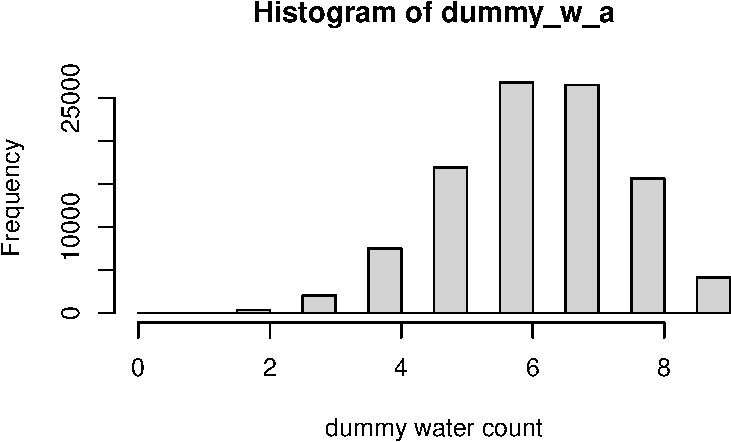
\includegraphics{03-sampling-the-imaginary_files/figure-pdf/fig-plot-hist-figure-3.4-a-1.pdf}

}

\caption{\label{fig-plot-hist-figure-3.4-a}Distribution of simulated
sample observations from 9 tosses of the globe. These samples assume the
proportion of water is 0.7. The plot usees the base R \texttt{hist()}
function}

\end{figure}

\begin{Shaded}
\begin{Highlighting}[]
\InformationTok{\textasciigrave{}\textasciigrave{}\textasciigrave{}\{r\}}
\CommentTok{\#| label: fig{-}plot{-}simplehist{-}figure{-}3.4{-}a}
\CommentTok{\#| fig{-}cap: "Distribution of simulated sample observations from 9 tosses of the globe. These samples assume the proportion of water is 0.7. the plot uses the rethinking::simplehist() function"}

\FunctionTok{set.seed}\NormalTok{(}\DecValTok{3}\NormalTok{)}
\DocumentationTok{\#\# R code 3.24}
\NormalTok{dummy\_w\_a }\OtherTok{\textless{}{-}} \FunctionTok{rbinom}\NormalTok{(}\FloatTok{1e5}\NormalTok{, }\AttributeTok{size =} \DecValTok{9}\NormalTok{, }\AttributeTok{prob =} \FloatTok{0.7}\NormalTok{)}
\NormalTok{rethinking}\SpecialCharTok{::}\FunctionTok{simplehist}\NormalTok{(dummy\_w\_a, }\AttributeTok{xlab =} \StringTok{"dummy water count"}\NormalTok{)}
\InformationTok{\textasciigrave{}\textasciigrave{}\textasciigrave{}}
\end{Highlighting}
\end{Shaded}

\begin{figure}[H]

{\centering 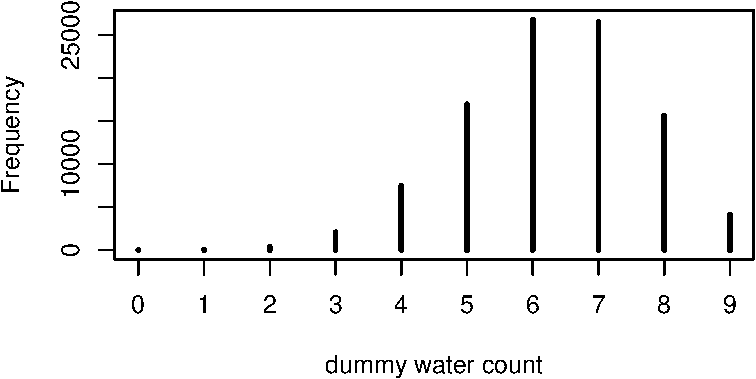
\includegraphics{03-sampling-the-imaginary_files/figure-pdf/fig-plot-simplehist-figure-3.4-a-1.pdf}

}

\caption{\label{fig-plot-simplehist-figure-3.4-a}Distribution of
simulated sample observations from 9 tosses of the globe. These samples
assume the proportion of water is 0.7. the plot uses the
rethinking::simplehist() function}

\end{figure}

\begin{quote}
Notice that most of the time the expected observation does not contain
water in its true proportion, 0.7. That's the nature of observation:
There is a one-to-many relationship between data and data-generating
processes. You should experiment with sample size, the \texttt{size}
input in the code above, as well as the prob, to see how the
distribution of simulated samples changes shape and location.
\end{quote}

\begin{quote}
Many readers will already have seen simulated observations.
\textbf{SAMPLING DISTRIBUTIONS} are the foundation of common
non-Bayesian statistical traditions. In those approaches, inference
about parameters is made through the sampling distribution. In this
book, inference about parameters is never done directly through a
sampling distribution. The posterior distribution is not sampled, but
deduced logically. Then samples can be drawn from the posterior, as
earlier in this chapter, to aid in inference. In neither case is
``sampling'' a physical act. In both cases, it's just a mathematical
device and produces only \emph{small world}
(Chapter~\ref{sec-small-and-large-worlds}) numbers.
\end{quote}

\hypertarget{model-checking}{%
\subsubsection{Model checking}\label{model-checking}}

\begin{quote}
MODEL CHECKING means (1) ensuring the model fitting worked correctly and
(2) evaluating the adequacy of a model for some purpose. Since Bayesian
models are always \emph{generative}, able to simulate observations as
well as estimate parameters from observations, once you condition a
model on data, you can simulate to examine the model's empirical
expectations.
\end{quote}

\begin{quote}
We'd like to \emph{propagate} the parameter uncertainty---carry it
forward---as we evaluate the implied predictions. All that is required
is averaging over the posterior density for \texttt{p}, while computing
the predictions. For each possible value of the parameter \texttt{p},
there is an implied distribution of outcomes. So if you were to compute
the sampling distribution of outcomes at each value of \texttt{p}, then
you could average all of these prediction distributions together, using
the posterior probabilities of each value of \texttt{p}, to get a
POSTERIOR PREDICTIVE DISTRIBUTION.
\end{quote}

The reproduction of FIGURE 3.6 that illustrates this averaging is shown
in ref\#\#\#.

\begin{quote}
we need to learn how to combine sampling of simulated observations, as
in the previous section, with sampling parameters from the posterior
distribution. We expect to do better when we use the entire posterior
distribution, not just some point estimate derived from it.
\end{quote}

So how do you actually do the calculations?

\begin{Shaded}
\begin{Highlighting}[]
\InformationTok{\textasciigrave{}\textasciigrave{}\textasciigrave{}\{r\}}
\CommentTok{\#| label: sim{-}pred{-}value{-}a}

\FunctionTok{set.seed}\NormalTok{(}\DecValTok{3}\NormalTok{)}
\DocumentationTok{\#\# R code 3.25}
\NormalTok{w\_a }\OtherTok{\textless{}{-}} \FunctionTok{rbinom}\NormalTok{(}\FloatTok{1e4}\NormalTok{, }\AttributeTok{size =} \DecValTok{9}\NormalTok{, }\AttributeTok{prob =} \FloatTok{0.6}\NormalTok{)}
\NormalTok{rethinking}\SpecialCharTok{::}\FunctionTok{simplehist}\NormalTok{(w\_a)}
\InformationTok{\textasciigrave{}\textasciigrave{}\textasciigrave{}}
\end{Highlighting}
\end{Shaded}

\begin{figure}[H]

{\centering 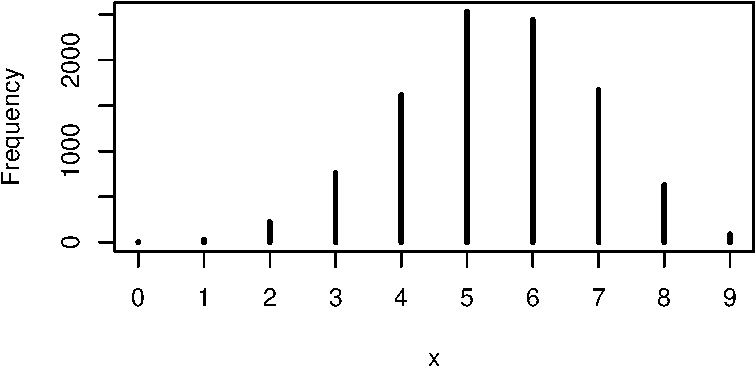
\includegraphics{03-sampling-the-imaginary_files/figure-pdf/sim-pred-value-a-1.pdf}

}

\end{figure}

\begin{quote}
This generates 10,000 (1e4) simulated predictions of 9 globe tosses
(size=9), assuming \(p = 6\). The predictions are stored as counts of
water, so the theoretical minimum is zero and the theoretical maximum is
nine.
\end{quote}

We used \texttt{rethinking::}simplehist(w\_a)` to get a clean histogram
of the simulated outcomes.

\begin{quote}
All you need to propagate parameter uncertainty into these predictions
is replace the value 0.6 with samples from the posterior:
\end{quote}

\begin{codelisting}

\caption{Generate 1e4 random binomial samples to simulate predicted
observations for \(p = 0.6\)}

\hypertarget{lst-sim-pred-samples-a}{%
\label{lst-sim-pred-samples-a}}%
\begin{Shaded}
\begin{Highlighting}[]
\InformationTok{\textasciigrave{}\textasciigrave{}\textasciigrave{}\{r\}}
\CommentTok{\#| label: sim{-}pred{-}samples{-}a}
\CommentTok{\#| fig{-}cap: "Random binomial samples to simulate predicted observations for $p = 0.6$"}
\CommentTok{\#| attr{-}source: \textquotesingle{}\#lst{-}sim{-}pred{-}samples{-}a lst{-}cap="Generate 1e4 random binomial samples to simulate predicted observations for $p = 0.6$"\textquotesingle{}}

\FunctionTok{set.seed}\NormalTok{(}\DecValTok{3}\NormalTok{)}
\DocumentationTok{\#\# R code 3.26}
\NormalTok{w2\_a }\OtherTok{\textless{}{-}} \FunctionTok{rbinom}\NormalTok{(}\FloatTok{1e4}\NormalTok{, }\AttributeTok{size =} \DecValTok{9}\NormalTok{, }\AttributeTok{prob =}\NormalTok{ samples\_a)}
\NormalTok{rethinking}\SpecialCharTok{::}\FunctionTok{simplehist}\NormalTok{(w2\_a)}
\InformationTok{\textasciigrave{}\textasciigrave{}\textasciigrave{}}
\end{Highlighting}
\end{Shaded}

\end{codelisting}

\begin{figure}[H]

{\centering 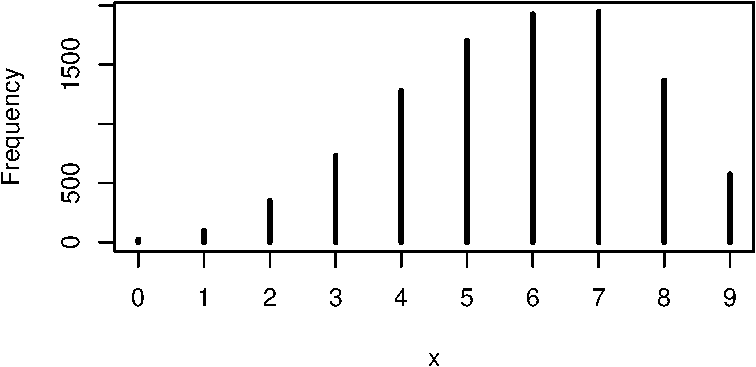
\includegraphics{03-sampling-the-imaginary_files/figure-pdf/sim-pred-samples-a-1.pdf}

}

\caption{Random binomial samples to simulate predicted observations for
\(p = 0.6\)}

\end{figure}

The symbol \texttt{samples\_a} above is the same list of random samples
from the posterior distribution that we have calculated in
Listing~\ref{lst-draw-samples-a} and used in previous sections.

\begin{quote}
For each sampled value, a random binomial observation is generated.
Since the sampled values appear in proportion to their posterior
probabilities, the resulting simulated observations are averaged over
the posterior. You can manipulate these simulated observations just like
you manipulate samples from the posterior---you can compute intervals
and point statistics using the same procedures.
\end{quote}

\begin{quote}
The simulated model predictions are quite consistent with the observed
data in this case---the actual count of 6 lies right in the middle of
the simulated distribution. \ldots{} So far, we've only viewed the data
just as the model views it: Each toss of the globe is completely
independent of the others. This assumption is questionable.
\end{quote}

\begin{quote}
So with the goal of seeking out aspects of prediction in which the model
fails, let's look at the data in two different ways. Recall that the
sequence of nine tosses was \texttt{W\ L\ W\ W\ W\ L\ W\ L\ W}. First,
consider the length of the longest run of either water or land. This
will provide a crude measure of correlation between tosses. So in the
observed data, the longest run is 3 W's. Second, consider the number of
times in the data that the sample switches from water to land or from
land to water. This is another measure of correlation between samples.
In the observed data, the number of switches is 6. There is nothing
special about these two new ways of describing the data. They just serve
to inspect the data in new ways. In your own modeling, you'll have to
imagine aspects of the data that are relevant in your context, for your
purposes.
\end{quote}

FIGURE 3.7 showing the simulated predictions, viewed in these two new
ways, is reproduced in ref\#\#\#. I have also postponed the
interpretation of Figure 3.7 to ref\#\#\#, because it is more
understandable viewing the plots.

\hypertarget{tidyverse-14}{%
\subsection{Tidyverse}\label{tidyverse-14}}

\begin{quote}
Dummy data for the globe tossing model arise from the binomial
likelihood. \ldots{}
\end{quote}

\hypertarget{i-stopped-here-2023-07-29}{%
\section{I STOPPED HERE! (2023-07-29)}\label{i-stopped-here-2023-07-29}}

\hypertarget{practice-with-brms}{%
\section{Practice with brms}\label{practice-with-brms}}

\begin{Shaded}
\begin{Highlighting}[]
\InformationTok{\textasciigrave{}\textasciigrave{}\textasciigrave{}\{r\}}
\FunctionTok{library}\NormalTok{(brms)}
\InformationTok{\textasciigrave{}\textasciigrave{}\textasciigrave{}}
\end{Highlighting}
\end{Shaded}

\begin{verbatim}
#> Loading required package: Rcpp
#> Loading 'brms' package (version 2.19.0). Useful instructions
#> can be found by typing help('brms'). A more detailed introduction
#> to the package is available through vignette('brms_overview').
#> 
#> Attaching package: 'brms'
#> The following object is masked from 'package:stats':
#> 
#>     ar
\end{verbatim}

\begin{Shaded}
\begin{Highlighting}[]
\InformationTok{\textasciigrave{}\textasciigrave{}\textasciigrave{}\{r\}}
\NormalTok{b3}\FloatTok{.1} \OtherTok{\textless{}{-}}
\NormalTok{  brms}\SpecialCharTok{::}\FunctionTok{brm}\NormalTok{(}\AttributeTok{data =} \FunctionTok{list}\NormalTok{(}\AttributeTok{w =} \DecValTok{6}\NormalTok{), }
      \AttributeTok{family =} \FunctionTok{binomial}\NormalTok{(}\AttributeTok{link =} \StringTok{"identity"}\NormalTok{),}
\NormalTok{      w }\SpecialCharTok{|} \FunctionTok{trials}\NormalTok{(}\DecValTok{9}\NormalTok{) }\SpecialCharTok{\textasciitilde{}} \DecValTok{0} \SpecialCharTok{+}\NormalTok{ Intercept,}
      \CommentTok{\# this is a flat prior}
\NormalTok{      brms}\SpecialCharTok{::}\FunctionTok{prior}\NormalTok{(}\FunctionTok{beta}\NormalTok{(}\DecValTok{1}\NormalTok{, }\DecValTok{1}\NormalTok{), }\AttributeTok{class =}\NormalTok{ b, }\AttributeTok{lb =} \DecValTok{0}\NormalTok{, }\AttributeTok{ub =} \DecValTok{1}\NormalTok{),}
      \AttributeTok{iter =} \DecValTok{5000}\NormalTok{, }\AttributeTok{warmup =} \DecValTok{1000}\NormalTok{,}
      \AttributeTok{seed =} \DecValTok{3}\NormalTok{,}
      \AttributeTok{file =} \StringTok{"fits/b03.01"}\NormalTok{)}
\InformationTok{\textasciigrave{}\textasciigrave{}\textasciigrave{}}
\end{Highlighting}
\end{Shaded}

We'll learn more about the beta distribution in Chapter 12. But for now,
here's the posterior summary for \texttt{b\_Intercept}, the probability
of a ``w''.

\begin{Shaded}
\begin{Highlighting}[]
\InformationTok{\textasciigrave{}\textasciigrave{}\textasciigrave{}\{r\}}
\NormalTok{brms}\SpecialCharTok{::}\FunctionTok{posterior\_summary}\NormalTok{(b3}\FloatTok{.1}\NormalTok{)[}\StringTok{"b\_Intercept"}\NormalTok{, ] }\SpecialCharTok{\%\textgreater{}\%} 
  \FunctionTok{round}\NormalTok{(}\AttributeTok{digits =} \DecValTok{2}\NormalTok{)}
\InformationTok{\textasciigrave{}\textasciigrave{}\textasciigrave{}}
\end{Highlighting}
\end{Shaded}

\begin{verbatim}
#>  Estimate Est.Error      Q2.5     Q97.5 
#>      0.64      0.14      0.34      0.88
\end{verbatim}

\begin{Shaded}
\begin{Highlighting}[]
\InformationTok{\textasciigrave{}\textasciigrave{}\textasciigrave{}\{r\}}
\NormalTok{f }\OtherTok{\textless{}{-}}
\NormalTok{  brms}\SpecialCharTok{:::}\FunctionTok{fitted.brmsfit}\NormalTok{(b3}\FloatTok{.1}\NormalTok{, }
         \AttributeTok{summary =}\NormalTok{ F,}
         \AttributeTok{scale =} \StringTok{"linear"}\NormalTok{) }\SpecialCharTok{\%\textgreater{}\%} 
  \FunctionTok{data.frame}\NormalTok{() }\SpecialCharTok{\%\textgreater{}\%} 
  \FunctionTok{set\_names}\NormalTok{(}\StringTok{"p"}\NormalTok{)}

\FunctionTok{glimpse}\NormalTok{(f)}
\InformationTok{\textasciigrave{}\textasciigrave{}\textasciigrave{}}
\end{Highlighting}
\end{Shaded}

\begin{verbatim}
#> Rows: 16,000
#> Columns: 1
#> $ p <dbl> 0.6318994, 0.8105015, 0.7677781, 0.7250286, 0.7265799, 0.7376768, 0.~
\end{verbatim}

\begin{Shaded}
\begin{Highlighting}[]
\InformationTok{\textasciigrave{}\textasciigrave{}\textasciigrave{}\{r\}}
\NormalTok{f }\SpecialCharTok{\%\textgreater{}\%} 
  \FunctionTok{ggplot}\NormalTok{(}\FunctionTok{aes}\NormalTok{(}\AttributeTok{x =}\NormalTok{ p)) }\SpecialCharTok{+}
  \FunctionTok{geom\_density}\NormalTok{(}\AttributeTok{fill =} \StringTok{"grey50"}\NormalTok{, }\AttributeTok{color =} \StringTok{"grey50"}\NormalTok{) }\SpecialCharTok{+}
  \FunctionTok{annotate}\NormalTok{(}\AttributeTok{geom =} \StringTok{"text"}\NormalTok{, }\AttributeTok{x =}\NormalTok{ .}\DecValTok{08}\NormalTok{, }\AttributeTok{y =} \FloatTok{2.5}\NormalTok{,}
           \AttributeTok{label =} \StringTok{"Posterior probability"}\NormalTok{) }\SpecialCharTok{+}
  \FunctionTok{scale\_x\_continuous}\NormalTok{(}\StringTok{"probability of water"}\NormalTok{,}
                     \AttributeTok{breaks =} \FunctionTok{c}\NormalTok{(}\DecValTok{0}\NormalTok{, .}\DecValTok{5}\NormalTok{, }\DecValTok{1}\NormalTok{),}
                     \AttributeTok{limits =} \DecValTok{0}\SpecialCharTok{:}\DecValTok{1}\NormalTok{) }\SpecialCharTok{+}
  \FunctionTok{scale\_y\_continuous}\NormalTok{(}\ConstantTok{NULL}\NormalTok{, }\AttributeTok{breaks =} \ConstantTok{NULL}\NormalTok{) }\SpecialCharTok{+}
  \FunctionTok{theme}\NormalTok{(}\AttributeTok{panel.grid =} \FunctionTok{element\_blank}\NormalTok{())}
\InformationTok{\textasciigrave{}\textasciigrave{}\textasciigrave{}}
\end{Highlighting}
\end{Shaded}

\begin{figure}[H]

{\centering 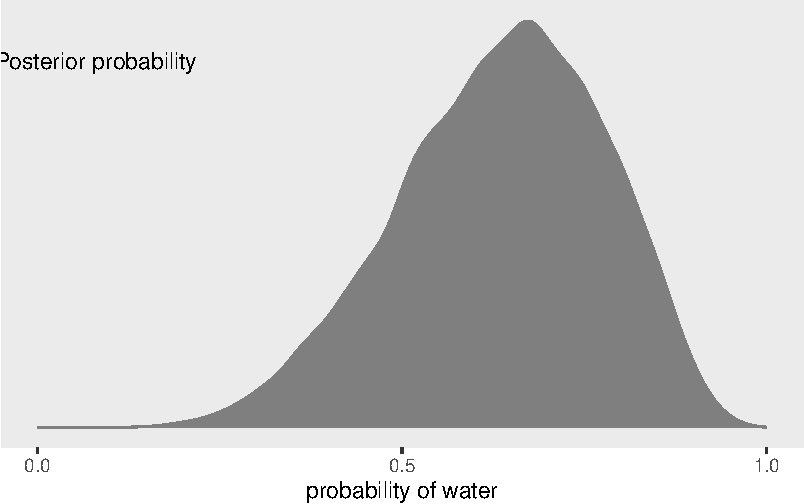
\includegraphics{03-sampling-the-imaginary_files/figure-pdf/unnamed-chunk-93-1.pdf}

}

\end{figure}

\begin{Shaded}
\begin{Highlighting}[]
\InformationTok{\textasciigrave{}\textasciigrave{}\textasciigrave{}\{r\}}
\CommentTok{\# the simulation}
\FunctionTok{set.seed}\NormalTok{(}\DecValTok{3}\NormalTok{)}

\NormalTok{f }\OtherTok{\textless{}{-}}
\NormalTok{  f }\SpecialCharTok{\%\textgreater{}\%} 
  \FunctionTok{mutate}\NormalTok{(}\AttributeTok{w =} \FunctionTok{rbinom}\NormalTok{(}\FunctionTok{n}\NormalTok{(), }\AttributeTok{size =} \DecValTok{9}\NormalTok{,  }\AttributeTok{prob =}\NormalTok{ p))}

\CommentTok{\# the plot}
\NormalTok{f }\SpecialCharTok{\%\textgreater{}\%} 
  \FunctionTok{ggplot}\NormalTok{(}\FunctionTok{aes}\NormalTok{(}\AttributeTok{x =}\NormalTok{ w)) }\SpecialCharTok{+}
  \FunctionTok{geom\_histogram}\NormalTok{(}\AttributeTok{binwidth =} \DecValTok{1}\NormalTok{, }\AttributeTok{center =} \DecValTok{0}\NormalTok{,}
                 \AttributeTok{color =} \StringTok{"grey92"}\NormalTok{, }\AttributeTok{linewidth =} \DecValTok{1}\SpecialCharTok{/}\DecValTok{10}\NormalTok{) }\SpecialCharTok{+}
  \FunctionTok{scale\_x\_continuous}\NormalTok{(}\StringTok{"number of water samples"}\NormalTok{, }\AttributeTok{breaks =} \DecValTok{0}\SpecialCharTok{:}\DecValTok{3} \SpecialCharTok{*} \DecValTok{3}\NormalTok{) }\SpecialCharTok{+}
  \FunctionTok{scale\_y\_continuous}\NormalTok{(}\ConstantTok{NULL}\NormalTok{, }\AttributeTok{breaks =} \ConstantTok{NULL}\NormalTok{, }\AttributeTok{limits =} \FunctionTok{c}\NormalTok{(}\DecValTok{0}\NormalTok{, }\DecValTok{5000}\NormalTok{)) }\SpecialCharTok{+}
  \FunctionTok{ggtitle}\NormalTok{(}\StringTok{"Posterior predictive distribution"}\NormalTok{) }\SpecialCharTok{+}
  \FunctionTok{coord\_cartesian}\NormalTok{(}\AttributeTok{xlim =} \FunctionTok{c}\NormalTok{(}\DecValTok{0}\NormalTok{, }\DecValTok{9}\NormalTok{)) }\SpecialCharTok{+}
  \FunctionTok{theme}\NormalTok{(}\AttributeTok{panel.grid =} \FunctionTok{element\_blank}\NormalTok{())}
\InformationTok{\textasciigrave{}\textasciigrave{}\textasciigrave{}}
\end{Highlighting}
\end{Shaded}

\begin{figure}[H]

{\centering 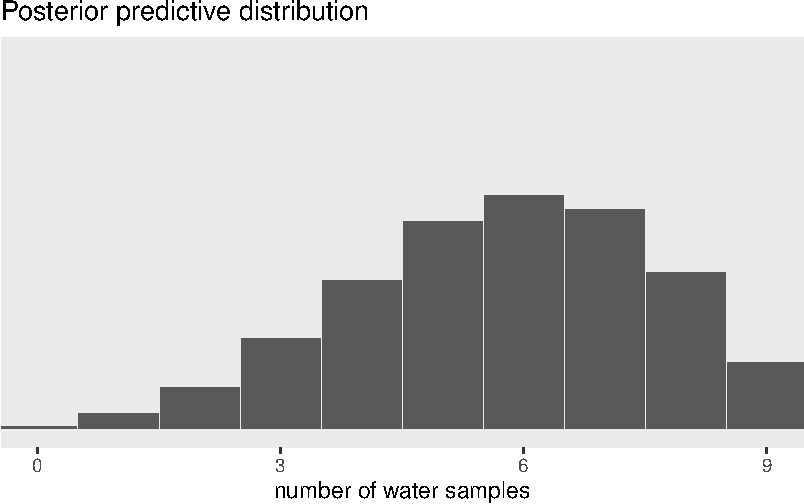
\includegraphics{03-sampling-the-imaginary_files/figure-pdf/unnamed-chunk-94-1.pdf}

}

\end{figure}

\hypertarget{session-info}{%
\section{Session info}\label{session-info}}

\begin{Shaded}
\begin{Highlighting}[]
\InformationTok{\textasciigrave{}\textasciigrave{}\textasciigrave{}\{r\}}
\CommentTok{\#| label: session{-}info}

\FunctionTok{sessionInfo}\NormalTok{()}
\InformationTok{\textasciigrave{}\textasciigrave{}\textasciigrave{}}
\end{Highlighting}
\end{Shaded}

\begin{verbatim}
#> R version 4.3.1 (2023-06-16)
#> Platform: x86_64-apple-darwin20 (64-bit)
#> Running under: macOS Ventura 13.4.1
#> 
#> Matrix products: default
#> BLAS:   /Library/Frameworks/R.framework/Versions/4.3-x86_64/Resources/lib/libRblas.0.dylib 
#> LAPACK: /Library/Frameworks/R.framework/Versions/4.3-x86_64/Resources/lib/libRlapack.dylib;  LAPACK version 3.11.0
#> 
#> locale:
#> [1] en_US.UTF-8/en_US.UTF-8/en_US.UTF-8/C/en_US.UTF-8/en_US.UTF-8
#> 
#> time zone: Europe/Vienna
#> tzcode source: internal
#> 
#> attached base packages:
#> [1] stats     graphics  grDevices utils     datasets  methods   base     
#> 
#> other attached packages:
#>  [1] brms_2.19.0     Rcpp_1.0.11     patchwork_1.1.2 lubridate_1.9.2
#>  [5] forcats_1.0.0   stringr_1.5.0   dplyr_1.1.2     purrr_1.0.1    
#>  [9] readr_2.1.4     tidyr_1.3.0     tibble_3.2.1    ggplot2_3.4.2  
#> [13] tidyverse_2.0.0
#> 
#> loaded via a namespace (and not attached):
#>   [1] tensorA_0.36.2       rstudioapi_0.15.0    jsonlite_1.8.7      
#>   [4] shape_1.4.6          magrittr_2.0.3       TH.data_1.1-2       
#>   [7] estimability_1.4.1   farver_2.1.1         nloptr_2.0.3        
#>  [10] rmarkdown_2.23       vctrs_0.6.3          minqa_1.2.5         
#>  [13] base64enc_0.1-3      htmltools_0.5.5      distributional_0.3.2
#>  [16] curl_5.0.1           tidybayes_3.0.4      StanHeaders_2.26.27 
#>  [19] htmlwidgets_1.6.2    plyr_1.8.8           sandwich_3.0-2      
#>  [22] emmeans_1.8.7        zoo_1.8-12           igraph_1.5.0.1      
#>  [25] mime_0.12            lifecycle_1.0.3      pkgconfig_2.0.3     
#>  [28] colourpicker_1.2.0   Matrix_1.6-0         R6_2.5.1            
#>  [31] fastmap_1.1.1        shiny_1.7.4.1        digest_0.6.33       
#>  [34] colorspace_2.1-0     ps_1.7.5             crosstalk_1.2.0     
#>  [37] projpred_2.6.0       labeling_0.4.2       fansi_1.0.4         
#>  [40] timechange_0.2.0     abind_1.4-5          mgcv_1.9-0          
#>  [43] compiler_4.3.1       withr_2.5.0          backports_1.4.1     
#>  [46] inline_0.3.19        shinystan_2.6.0      rethinking_2.31     
#>  [49] gamm4_0.2-6          pkgbuild_1.4.2       MASS_7.3-60         
#>  [52] gtools_3.9.4         loo_2.6.0            tools_4.3.1         
#>  [55] httpuv_1.6.11        threejs_0.3.3        glue_1.6.2          
#>  [58] callr_3.7.3          nlme_3.1-162         promises_1.2.0.1    
#>  [61] grid_4.3.1           cmdstanr_0.5.3       checkmate_2.2.0     
#>  [64] reshape2_1.4.4       generics_0.1.3       gtable_0.3.3        
#>  [67] tzdb_0.4.0           hms_1.1.3            xml2_1.3.5          
#>  [70] utf8_1.2.3           pillar_1.9.0         ggdist_3.3.0        
#>  [73] markdown_1.7         posterior_1.4.1      later_1.3.1         
#>  [76] splines_4.3.1        lattice_0.21-8       survival_3.5-5      
#>  [79] tidyselect_1.2.0     miniUI_0.1.1.1       knitr_1.43          
#>  [82] arrayhelpers_1.1-0   gridExtra_2.3        V8_4.3.3            
#>  [85] rversions_2.1.2      stats4_4.3.1         xfun_0.39           
#>  [88] bridgesampling_1.1-2 matrixStats_1.0.0    DT_0.28             
#>  [91] rstan_2.26.22        stringi_1.7.12       yaml_2.3.7          
#>  [94] boot_1.3-28.1        evaluate_0.21        codetools_0.2-19    
#>  [97] cli_3.6.1            RcppParallel_5.1.7   shinythemes_1.2.0   
#> [100] xtable_1.8-4         munsell_0.5.0        processx_3.8.2      
#> [103] coda_0.19-4          svUnit_1.0.6         parallel_4.3.1      
#> [106] rstantools_2.3.1.1   ellipsis_0.3.2       prettyunits_1.1.1   
#> [109] dygraphs_1.1.1.6     bayesplot_1.10.0     Brobdingnag_1.2-9   
#> [112] lme4_1.1-34          mvtnorm_1.2-2        scales_1.2.1        
#> [115] xts_0.13.1           crayon_1.5.2         rlang_1.1.1         
#> [118] multcomp_1.4-25      shinyjs_2.1.0
\end{verbatim}

\bookmarksetup{startatroot}

\hypertarget{a-geocentric-models}{%
\chapter{4a: Geocentric Models}\label{a-geocentric-models}}

\begin{Shaded}
\begin{Highlighting}[]
\InformationTok{\textasciigrave{}\textasciigrave{}\textasciigrave{}\{r\}}
\CommentTok{\#| label: setup}

\FunctionTok{library}\NormalTok{(conflicted)}
\FunctionTok{library}\NormalTok{(rethinking)}
\InformationTok{\textasciigrave{}\textasciigrave{}\textasciigrave{}}
\end{Highlighting}
\end{Shaded}

\begin{verbatim}
#> Loading required package: rstan
#> Loading required package: StanHeaders
#> 
#> rstan version 2.26.22 (Stan version 2.26.1)
#> For execution on a local, multicore CPU with excess RAM we recommend calling
#> options(mc.cores = parallel::detectCores()).
#> To avoid recompilation of unchanged Stan programs, we recommend calling
#> rstan_options(auto_write = TRUE)
#> For within-chain threading using `reduce_sum()` or `map_rect()` Stan functions,
#> change `threads_per_chain` option:
#> rstan_options(threads_per_chain = 1)
#> Loading required package: cmdstanr
#> This is cmdstanr version 0.5.3
#> - CmdStanR documentation and vignettes: mc-stan.org/cmdstanr
#> - CmdStan path: /Users/petzi/.cmdstan/cmdstan-2.32.2
#> - CmdStan version: 2.32.2
#> Loading required package: parallel
#> rethinking (Version 2.31)
\end{verbatim}

\begin{Shaded}
\begin{Highlighting}[]
\InformationTok{\textasciigrave{}\textasciigrave{}\textasciigrave{}\{r\}}
\CommentTok{\#| label: setup}

\FunctionTok{library}\NormalTok{(tidyverse)}
\InformationTok{\textasciigrave{}\textasciigrave{}\textasciigrave{}}
\end{Highlighting}
\end{Shaded}

\begin{verbatim}
#> -- Attaching core tidyverse packages ------------------------ tidyverse 2.0.0 --
#> v dplyr     1.1.2     v readr     2.1.4
#> v forcats   1.0.0     v stringr   1.5.0
#> v ggplot2   3.4.2     v tibble    3.2.1
#> v lubridate 1.9.2     v tidyr     1.3.0
#> v purrr     1.0.1
\end{verbatim}

\begin{Shaded}
\begin{Highlighting}[]
\InformationTok{\textasciigrave{}\textasciigrave{}\textasciigrave{}\{r\}}
\CommentTok{\#| label: setup}

\FunctionTok{library}\NormalTok{(brms)}
\InformationTok{\textasciigrave{}\textasciigrave{}\textasciigrave{}}
\end{Highlighting}
\end{Shaded}

\begin{verbatim}
#> Loading required package: Rcpp
#> Loading 'brms' package (version 2.19.0). Useful instructions
#> can be found by typing help('brms'). A more detailed introduction
#> to the package is available through vignette('brms_overview').
\end{verbatim}

\begin{Shaded}
\begin{Highlighting}[]
\InformationTok{\textasciigrave{}\textasciigrave{}\textasciigrave{}\{r\}}
\CommentTok{\#| label: setup}

\FunctionTok{library}\NormalTok{(skimr)}

\FunctionTok{conflicts\_prefer}\NormalTok{(dplyr}\SpecialCharTok{::}\NormalTok{filter)}
\InformationTok{\textasciigrave{}\textasciigrave{}\textasciigrave{}}
\end{Highlighting}
\end{Shaded}

\begin{verbatim}
#> [conflicted] Will prefer dplyr::filter over any other package.
\end{verbatim}

\hypertarget{a-normal-distributions}{%
\section{4.1a Normal Distributions}\label{a-normal-distributions}}

\hypertarget{a-normal-by-addition}{%
\subsection{4.1.1a Normal by addition}\label{a-normal-by-addition}}

\begin{quote}
Suppose you and a thousand of your closest friends line up on the
halfway line of a soccer field (football pitch). Each of you has a coin
in your hand. At the sound of the whistle, you begin flipping the coins.
Each time a coin comes up heads, that person moves one step towards the
left-hand goal. Each time a coin comes up tails, that person moves one
step towards the right-hand goal. Each person flips the coin 16 times,
follows the implied moves, and then stands still. Now we measure the
distance of each person from the halfway line. Can you predict what
proportion of the thousand people who are standing on the halfway line?
How about the proportion 5 yards left of the line?
\end{quote}

Showing that there's nothing special about the underlying coin flip:

\begin{quote}
Assume \ldots{} that each step is different from all the others, a
random distance between zero and one yard. Thus a coin is flipped, a
distance between zero and one yard is taken in the indicated direction,
and the process repeats. To simulate this, we generate for each person a
list of 16 random numbers between −1 and 1. These are the individual
steps. Then we add these steps together to get the position after 16
steps. Then we need to replicate this procedure 1000 times.
\end{quote}

\begin{Shaded}
\begin{Highlighting}[]
\InformationTok{\textasciigrave{}\textasciigrave{}\textasciigrave{}\{r\}}
\CommentTok{\#| label: sim{-}step{-}experiment{-}a}

\CommentTok{\# to replicate with the b{-}model}
\FunctionTok{set.seed}\NormalTok{(}\DecValTok{4}\NormalTok{)}

\DocumentationTok{\#\# R code 4.1}
\NormalTok{pos\_a1 }\OtherTok{\textless{}{-}} \FunctionTok{replicate}\NormalTok{(}\DecValTok{1000}\NormalTok{, }\FunctionTok{sum}\NormalTok{(}\FunctionTok{runif}\NormalTok{(}\DecValTok{16}\NormalTok{, }\SpecialCharTok{{-}}\DecValTok{1}\NormalTok{, }\DecValTok{1}\NormalTok{)))}
\NormalTok{pos\_a2 }\OtherTok{\textless{}{-}} \FunctionTok{replicate}\NormalTok{(}\DecValTok{1000}\NormalTok{, }\FunctionTok{sum}\NormalTok{(}\FunctionTok{runif}\NormalTok{(}\DecValTok{32}\NormalTok{, }\SpecialCharTok{{-}}\DecValTok{1}\NormalTok{, }\DecValTok{1}\NormalTok{)))}

\FunctionTok{par}\NormalTok{(}\AttributeTok{mfrow =} \FunctionTok{c}\NormalTok{(}\DecValTok{2}\NormalTok{, }\DecValTok{2}\NormalTok{)) }\CommentTok{\# 2{-}by{-}2 grid of plots}
\FunctionTok{hist}\NormalTok{(pos\_a1)}
\FunctionTok{hist}\NormalTok{(pos\_a2)}

\FunctionTok{plot}\NormalTok{(}\FunctionTok{density}\NormalTok{(pos\_a1))}
\FunctionTok{plot}\NormalTok{(}\FunctionTok{density}\NormalTok{(pos\_a2))}
\InformationTok{\textasciigrave{}\textasciigrave{}\textasciigrave{}}
\end{Highlighting}
\end{Shaded}

\begin{figure}[H]

{\centering 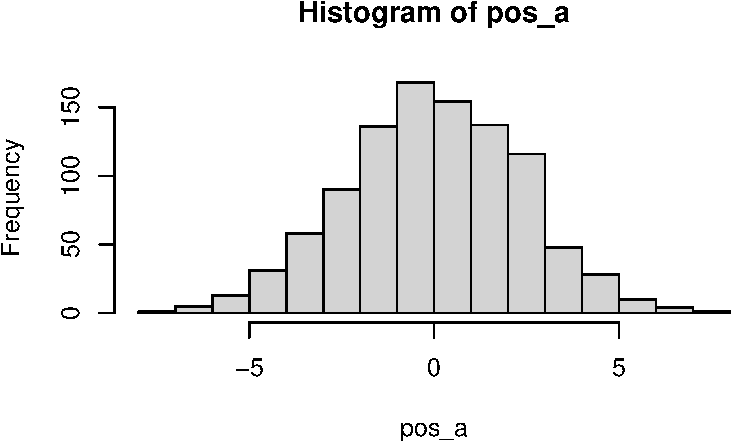
\includegraphics{04a-geocentric-models_files/figure-pdf/sim-step-experiment-a-1.pdf}

}

\end{figure}

\begin{quote}
Any process that adds together random values from the same distribution
converges to a normal. \ldots{} It doesn't matter what shape the
underlying distribution possesses. It could be uniform, like in our
example above, or it could be (nearly) anything else. Depending upon the
underlying distribution, the convergence might be slow, but it will be
inevitable.
\end{quote}

\hypertarget{a-normal-by-multiplication}{%
\subsection{4.1.2a Normal by
multiplication}\label{a-normal-by-multiplication}}

\begin{Shaded}
\begin{Highlighting}[]
\InformationTok{\textasciigrave{}\textasciigrave{}\textasciigrave{}\{r\}}
\CommentTok{\#| label: random{-}sample{-}growth}

\DocumentationTok{\#\# R code 4.2}
\FunctionTok{prod}\NormalTok{(}\DecValTok{1} \SpecialCharTok{+} \FunctionTok{runif}\NormalTok{(}\DecValTok{12}\NormalTok{, }\DecValTok{0}\NormalTok{, }\FloatTok{0.1}\NormalTok{))}
\InformationTok{\textasciigrave{}\textasciigrave{}\textasciigrave{}}
\end{Highlighting}
\end{Shaded}

\begin{verbatim}
#> [1] 1.819134
\end{verbatim}

\begin{Shaded}
\begin{Highlighting}[]
\InformationTok{\textasciigrave{}\textasciigrave{}\textasciigrave{}\{r\}}
\CommentTok{\#| label: normal{-}by{-}multiplaction}

\DocumentationTok{\#\# R code 4.3}
\NormalTok{growth }\OtherTok{\textless{}{-}} \FunctionTok{replicate}\NormalTok{(}\DecValTok{10000}\NormalTok{, }\FunctionTok{prod}\NormalTok{(}\DecValTok{1} \SpecialCharTok{+} \FunctionTok{runif}\NormalTok{(}\DecValTok{12}\NormalTok{, }\DecValTok{0}\NormalTok{, }\FloatTok{0.1}\NormalTok{)))}
\FunctionTok{dens}\NormalTok{(growth, }\AttributeTok{norm.comp =} \ConstantTok{TRUE}\NormalTok{)}
\InformationTok{\textasciigrave{}\textasciigrave{}\textasciigrave{}}
\end{Highlighting}
\end{Shaded}

\begin{figure}[H]

{\centering 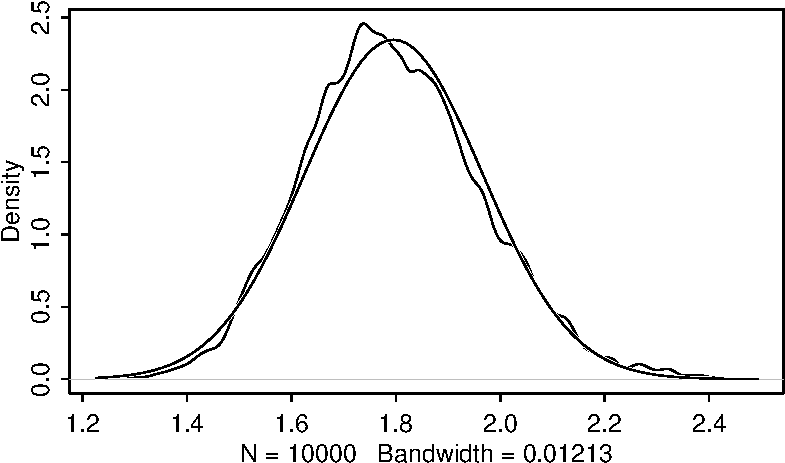
\includegraphics{04a-geocentric-models_files/figure-pdf/normal-by-multiplaction-1.pdf}

}

\end{figure}

\begin{quote}
\ldots{} small effects that multiply together are approximately
additive, and so they also tend to stabilize on Gaussian distributions.
\end{quote}

\begin{Shaded}
\begin{Highlighting}[]
\InformationTok{\textasciigrave{}\textasciigrave{}\textasciigrave{}\{r\}}
\CommentTok{\#| label: compare{-}small{-}big{-}growth}

\DocumentationTok{\#\# R code 4.4}
\NormalTok{big }\OtherTok{\textless{}{-}} \FunctionTok{replicate}\NormalTok{(}\DecValTok{10000}\NormalTok{, }\FunctionTok{prod}\NormalTok{(}\DecValTok{1} \SpecialCharTok{+} \FunctionTok{runif}\NormalTok{(}\DecValTok{12}\NormalTok{, }\DecValTok{0}\NormalTok{, }\FloatTok{0.5}\NormalTok{)))}
\NormalTok{small }\OtherTok{\textless{}{-}} \FunctionTok{replicate}\NormalTok{(}\DecValTok{10000}\NormalTok{, }\FunctionTok{prod}\NormalTok{(}\DecValTok{1} \SpecialCharTok{+} \FunctionTok{runif}\NormalTok{(}\DecValTok{12}\NormalTok{, }\DecValTok{0}\NormalTok{, }\FloatTok{0.01}\NormalTok{)))}

\FunctionTok{par}\NormalTok{(}\AttributeTok{mfrow =} \FunctionTok{c}\NormalTok{(}\DecValTok{2}\NormalTok{, }\DecValTok{2}\NormalTok{)) }\CommentTok{\# 2{-}by{-}2 grid of plots}
\FunctionTok{dens}\NormalTok{(big, }\AttributeTok{norm.comp =} \ConstantTok{TRUE}\NormalTok{)}
\FunctionTok{dens}\NormalTok{(small, }\AttributeTok{norm.comp =} \ConstantTok{TRUE}\NormalTok{)}
\InformationTok{\textasciigrave{}\textasciigrave{}\textasciigrave{}}
\end{Highlighting}
\end{Shaded}

\begin{figure}[H]

{\centering \includegraphics{04a-geocentric-models_files/figure-pdf/compare-small-big-growth-1.pdf}

}

\end{figure}

\begin{quote}
The interacting growth deviations, as long as they are sufficiently
small, converge to a Gaussian distribution. In this way, the range of
causal forces that tend towards Gaussian distributions extends well
beyond purely additive interactions.
\end{quote}

\hypertarget{a-normal-by-log-multiplication}{%
\subsection{4.1.3a Normal by
log-multiplication}\label{a-normal-by-log-multiplication}}

\begin{quote}
Large deviates that are multiplied together do not produce Gaussian
distributions, but they do tend to produce Gaussian distributions on the
log scale.
\end{quote}

\begin{Shaded}
\begin{Highlighting}[]
\InformationTok{\textasciigrave{}\textasciigrave{}\textasciigrave{}\{r\}}
\CommentTok{\#| label: normal{-}by{-}log{-}multi}

\DocumentationTok{\#\# R code 4.5}
\NormalTok{log.big }\OtherTok{\textless{}{-}} \FunctionTok{replicate}\NormalTok{(}\DecValTok{10000}\NormalTok{, }\FunctionTok{log}\NormalTok{(}\FunctionTok{prod}\NormalTok{(}\DecValTok{1} \SpecialCharTok{+} \FunctionTok{runif}\NormalTok{(}\DecValTok{12}\NormalTok{, }\DecValTok{0}\NormalTok{, }\FloatTok{0.5}\NormalTok{))))}

\FunctionTok{par}\NormalTok{(}\AttributeTok{mfrow =} \FunctionTok{c}\NormalTok{(}\DecValTok{2}\NormalTok{, }\DecValTok{2}\NormalTok{)) }\CommentTok{\# 2{-}by{-}2 grid of plots}
\FunctionTok{dens}\NormalTok{(big, }\AttributeTok{norm.comp =} \ConstantTok{TRUE}\NormalTok{)}
\FunctionTok{dens}\NormalTok{(log.big, }\AttributeTok{norm.comp =} \ConstantTok{TRUE}\NormalTok{)}
\InformationTok{\textasciigrave{}\textasciigrave{}\textasciigrave{}}
\end{Highlighting}
\end{Shaded}

\begin{figure}[H]

{\centering \includegraphics{04a-geocentric-models_files/figure-pdf/normal-by-log-multi-1.pdf}

}

\end{figure}

\begin{quote}
We get the Gaussian distribution back, because adding logs is equivalent
to multiplying the original numbers. So even multiplicative interactions
of large deviations can produce Gaussian distributions, once we measure
the outcomes on the log scale. Since measurement scales are arbitrary,
there's nothing suspicious about this transformation.
\end{quote}

\hypertarget{a-using-gaussian-distribution}{%
\subsection{4.1.4a Using Gaussian
Distribution}\label{a-using-gaussian-distribution}}

\textbf{Ontological Reasons}: the world is full of Gaussian
distributions, approximately. We're never going to experience a perfect
Gaussian distribution. But it is a widespread pattern, appearing again
and again at different scales and in different domains. \ldots{} The
Gaussian is a member of a family of fundamental natural distributions
known as the \textbf{EXPONENTIAL FAMILY}. All of the members of this
family are important for working science, because they populate our
world.

\textbf{Epistemological Reasons}: the Gaussian represents a particular
state of ignorance. When all we know or are willing to say about a
distribution of measures (measures are continuous values on the real
number line) is their mean and variance, then the Gaussian distribution
arises as the most consistent with our assumptions.

\begin{tcolorbox}[enhanced jigsaw, colframe=quarto-callout-tip-color-frame, colback=white, toprule=.15mm, breakable, arc=.35mm, bottomtitle=1mm, colbacktitle=quarto-callout-tip-color!10!white, toptitle=1mm, titlerule=0mm, title=\textcolor{quarto-callout-tip-color}{\faLightbulb}\hspace{0.5em}{Gaussian distribution}, leftrule=.75mm, opacityback=0, rightrule=.15mm, opacitybacktitle=0.6, bottomrule=.15mm, left=2mm, coltitle=black]

The Gaussian is a continuous distribution, unlike the discrete
distributions of earlier chapters. Probability distributions with only
discrete outcomes, like the binomial, are called \emph{probability mass}
functions and denoted \texttt{Pr}. Continuous ones like the Gaussian are
called \emph{probability density} functions, denoted with
\emph{\texttt{p}} or just plain old \emph{\texttt{f}}, depending upon
author and tradition. For mathematical reasons, probability densities
can be greater than 1. Try dnorm(0,0,0.1), for example, which is the way
to make R calculate \emph{\texttt{p}}\texttt{(0\textbar{}0,\ 0.1)}. The
answer, about 4, is no mistake. Probability \emph{density} is the rate
of change in cumulative probability. So where cumulative probability is
increasing rapidly, density can easily exceed 1. But if we calculate the
area under the density function, it will never exceed 1. Such areas are
also called \emph{probability mass}.

\end{tcolorbox}

\hypertarget{a-language-describing-models}{%
\section{4.2a Language describing
models}\label{a-language-describing-models}}

\begin{quote}
(1)~~First, we recognize a set of variables to work with. Some of these
variables are observable. We call these \emph{data}. Others are
unobservable things like rates and averages. We call these
\emph{parameters}.

(2)~~We define each variable either in terms of the other variables or
in terms of a probability distribution.

(3)~~The combination of variables and their probability distributions
defines a \emph{joint generative model} that can be used both to
simulate hypothetical observations as well as analyze real ones.
\end{quote}

\hypertarget{a-gaussian-model-of-height}{%
\section{4.3a Gaussian model of
height}\label{a-gaussian-model-of-height}}

\hypertarget{a-the-data}{%
\subsection{4.3.1a The data}\label{a-the-data}}

\begin{Shaded}
\begin{Highlighting}[]
\InformationTok{\textasciigrave{}\textasciigrave{}\textasciigrave{}\{r\}}
\CommentTok{\#| label: load{-}howell{-}data{-}a}

\DocumentationTok{\#\# R code 4.7}
\FunctionTok{data}\NormalTok{(Howell1)}
\NormalTok{d\_a }\OtherTok{\textless{}{-}}\NormalTok{ Howell1}
\InformationTok{\textasciigrave{}\textasciigrave{}\textasciigrave{}}
\end{Highlighting}
\end{Shaded}

\hypertarget{a-show-the-data}{%
\subsubsection{4.3.1.1a Show the data}\label{a-show-the-data}}

\begin{Shaded}
\begin{Highlighting}[]
\InformationTok{\textasciigrave{}\textasciigrave{}\textasciigrave{}\{r\}}
\CommentTok{\#| label: show{-}howell{-}data{-}a}

\DocumentationTok{\#\# R code 4.8}
\FunctionTok{str}\NormalTok{(d\_a)}

\DocumentationTok{\#\# R code 4.9}
\FunctionTok{precis}\NormalTok{(d\_a)}
\InformationTok{\textasciigrave{}\textasciigrave{}\textasciigrave{}}
\end{Highlighting}
\end{Shaded}

\begin{verbatim}
#> 'data.frame':    544 obs. of  4 variables:
#>  $ height: num  152 140 137 157 145 ...
#>  $ weight: num  47.8 36.5 31.9 53 41.3 ...
#>  $ age   : num  63 63 65 41 51 35 32 27 19 54 ...
#>  $ male  : int  1 0 0 1 0 1 0 1 0 1 ...
#>               mean         sd      5.5%     94.5%     histogram
#> height 138.2635963 27.6024476 81.108550 165.73500 ▁▁▁▁▁▁▁▂▁▇▇▅▁
#> weight  35.6106176 14.7191782  9.360721  54.50289 ▁▂▃▂▂▂▂▅▇▇▃▂▁
#> age     29.3443934 20.7468882  1.000000  66.13500     ▇▅▅▃▅▂▂▁▁
#> male     0.4724265  0.4996986  0.000000   1.00000    ▇▁▁▁▁▁▁▁▁▇
\end{verbatim}

\hypertarget{a-select-the-height-data-of-adults}{%
\subsubsection{4.3.1.2a Select the height data of
adults}\label{a-select-the-height-data-of-adults}}

\begin{Shaded}
\begin{Highlighting}[]
\InformationTok{\textasciigrave{}\textasciigrave{}\textasciigrave{}\{r\}}
\CommentTok{\#| label: select{-}height{-}adults{-}a}

\DocumentationTok{\#\# R code 4.10}
\FunctionTok{head}\NormalTok{(d\_a}\SpecialCharTok{$}\NormalTok{height)}
 
\DocumentationTok{\#\# R code 4.11}
\NormalTok{d2\_a }\OtherTok{\textless{}{-}}\NormalTok{ d\_a[d\_a}\SpecialCharTok{$}\NormalTok{age }\SpecialCharTok{\textgreater{}=} \DecValTok{18}\NormalTok{, ]}
\InformationTok{\textasciigrave{}\textasciigrave{}\textasciigrave{}}
\end{Highlighting}
\end{Shaded}

\begin{verbatim}
#> [1] 151.765 139.700 136.525 156.845 145.415 163.830
\end{verbatim}

\hypertarget{a-the-model}{%
\subsection{4.3.2a The model}\label{a-the-model}}

\begin{quote}
Our goal is to model these values using a Gaussian distribution.
\end{quote}

\hypertarget{a-plot-the-priors}{%
\subsubsection{4.3.2.1a Plot the priors}\label{a-plot-the-priors}}

\begin{Shaded}
\begin{Highlighting}[]
\InformationTok{\textasciigrave{}\textasciigrave{}\textasciigrave{}\{r\}}
\CommentTok{\#| label: print{-}height{-}dist}

\FunctionTok{dens}\NormalTok{(d2\_a}\SpecialCharTok{$}\NormalTok{height, }\AttributeTok{norm.comp =} \ConstantTok{TRUE}\NormalTok{)}
\InformationTok{\textasciigrave{}\textasciigrave{}\textasciigrave{}}
\end{Highlighting}
\end{Shaded}

\begin{figure}[H]

{\centering \includegraphics{04a-geocentric-models_files/figure-pdf/print-height-dist-1.pdf}

}

\end{figure}

\textbf{Plot the mu prior (mean)}

\begin{Shaded}
\begin{Highlighting}[]
\InformationTok{\textasciigrave{}\textasciigrave{}\textasciigrave{}\{r\}}
\CommentTok{\#| label: plot{-}mean{-}prior{-}a}

\DocumentationTok{\#\# R code 4.12}
\FunctionTok{curve}\NormalTok{(}\FunctionTok{dnorm}\NormalTok{(x, }\DecValTok{178}\NormalTok{, }\DecValTok{20}\NormalTok{), }\AttributeTok{from =} \DecValTok{100}\NormalTok{, }\AttributeTok{to =} \DecValTok{250}\NormalTok{)}
\InformationTok{\textasciigrave{}\textasciigrave{}\textasciigrave{}}
\end{Highlighting}
\end{Shaded}

\begin{figure}[H]

{\centering \includegraphics{04a-geocentric-models_files/figure-pdf/plot-mean-prior-a-1.pdf}

}

\end{figure}

\textbf{Plot the sigma prior (standard deviation)}

\begin{Shaded}
\begin{Highlighting}[]
\InformationTok{\textasciigrave{}\textasciigrave{}\textasciigrave{}\{r\}}
\CommentTok{\#| label: plot{-}sd{-}prior{-}a}

\DocumentationTok{\#\# R code 4.13}
\FunctionTok{curve}\NormalTok{(}\FunctionTok{dunif}\NormalTok{(x, }\DecValTok{0}\NormalTok{, }\DecValTok{50}\NormalTok{), }\AttributeTok{from =} \SpecialCharTok{{-}}\DecValTok{10}\NormalTok{, }\AttributeTok{to =} \DecValTok{60}\NormalTok{)}
\InformationTok{\textasciigrave{}\textasciigrave{}\textasciigrave{}}
\end{Highlighting}
\end{Shaded}

\begin{figure}[H]

{\centering \includegraphics{04a-geocentric-models_files/figure-pdf/plot-sd-prior-a-1.pdf}

}

\end{figure}

\hypertarget{a-prior-predictive-simulation}{%
\subsubsection{4.3.2.2a Prior predictive
simulation}\label{a-prior-predictive-simulation}}

\begin{quote}
Once you've chosen priors for \emph{h, μ}, and \emph{σ}, these imply a
joint prior distribution of individual heights. By simulating from this
distribution, you can see what your choices imply about observable
height. This helps you diagnose bad choices.
\end{quote}

\textbf{Simulate heights by sampling from the prior}

\begin{Shaded}
\begin{Highlighting}[]
\InformationTok{\textasciigrave{}\textasciigrave{}\textasciigrave{}\{r\}}
\CommentTok{\#| label: prior{-}predictive{-}sim{-}a}

\DocumentationTok{\#\# R code 4.14}
\NormalTok{sample\_mu\_a }\OtherTok{\textless{}{-}} \FunctionTok{rnorm}\NormalTok{(}\FloatTok{1e4}\NormalTok{, }\DecValTok{178}\NormalTok{, }\DecValTok{20}\NormalTok{)}
\NormalTok{sample\_sigma\_a }\OtherTok{\textless{}{-}} \FunctionTok{runif}\NormalTok{(}\FloatTok{1e4}\NormalTok{, }\DecValTok{0}\NormalTok{, }\DecValTok{50}\NormalTok{)}
\NormalTok{prior\_h\_a }\OtherTok{\textless{}{-}} \FunctionTok{rnorm}\NormalTok{(}\FloatTok{1e4}\NormalTok{, sample\_mu\_a, sample\_sigma\_a)}
\FunctionTok{dens}\NormalTok{(prior\_h\_a)}
\InformationTok{\textasciigrave{}\textasciigrave{}\textasciigrave{}}
\end{Highlighting}
\end{Shaded}

\begin{figure}[H]

{\centering \includegraphics{04a-geocentric-models_files/figure-pdf/prior-predictive-sim-a-1.pdf}

}

\end{figure}

Playing around with different priors coming from scientific background
knowledge about heights of adults:

\begin{Shaded}
\begin{Highlighting}[]
\InformationTok{\textasciigrave{}\textasciigrave{}\textasciigrave{}\{r\}}
\CommentTok{\#| label: prior2{-}predictive{-}sim{-}a}

\DocumentationTok{\#\# R code 4.14}
\NormalTok{sample\_mu2\_a }\OtherTok{\textless{}{-}} \FunctionTok{rnorm}\NormalTok{(}\FloatTok{1e4}\NormalTok{, }\DecValTok{170}\NormalTok{, }\DecValTok{20}\NormalTok{)}
\NormalTok{sample\_sigma2\_a }\OtherTok{\textless{}{-}} \FunctionTok{runif}\NormalTok{(}\FloatTok{1e4}\NormalTok{, }\DecValTok{0}\NormalTok{, }\DecValTok{35}\NormalTok{)}
\NormalTok{prior2\_h\_a }\OtherTok{\textless{}{-}} \FunctionTok{rnorm}\NormalTok{(}\FloatTok{1e4}\NormalTok{, sample\_mu2\_a, sample\_sigma2\_a)}
\FunctionTok{dens}\NormalTok{(prior2\_h\_a)}
\InformationTok{\textasciigrave{}\textasciigrave{}\textasciigrave{}}
\end{Highlighting}
\end{Shaded}

\begin{figure}[H]

{\centering \includegraphics{04a-geocentric-models_files/figure-pdf/prior2-predictive-sim-a-1.pdf}

}

\end{figure}

\textbf{Simulate heights from priors with large sd}

\begin{quote}
Priors with \ldots{} large standard deviations are quite common in
Bayesian models, but they are hardly ever sensible.
\end{quote}

\begin{Shaded}
\begin{Highlighting}[]
\InformationTok{\textasciigrave{}\textasciigrave{}\textasciigrave{}\{r\}}
\CommentTok{\#| label: plot{-}predictive{-}sim2{-}a}

\NormalTok{sample\_mu3\_a }\OtherTok{\textless{}{-}} \FunctionTok{rnorm}\NormalTok{(}\FloatTok{1e4}\NormalTok{, }\DecValTok{178}\NormalTok{, }\DecValTok{100}\NormalTok{)}
\NormalTok{prior\_h3\_a }\OtherTok{\textless{}{-}} \FunctionTok{rnorm}\NormalTok{(}\FloatTok{1e4}\NormalTok{, sample\_mu3\_a, sample\_sigma\_a)}
\FunctionTok{dens}\NormalTok{(prior\_h3\_a)}
\InformationTok{\textasciigrave{}\textasciigrave{}\textasciigrave{}}
\end{Highlighting}
\end{Shaded}

\begin{figure}[H]

{\centering \includegraphics{04a-geocentric-models_files/figure-pdf/plot-predictive-sim2-a-1.pdf}

}

\end{figure}

\hypertarget{a-personal-comment}{%
\subsubsection{4.3.2.3a Personal comment}\label{a-personal-comment}}

Both simulation show unsensitive data with negative height to the left
and gigantic humans in comparison to the tallest person ---
\href{https://en.wikipedia.org/wiki/Robert_Wadlow}{Robert Pershing
Wadlow} (1918--1940) --- ever measured (272cm).

So what? Are the priors chosen wrongly? Or does these impossibilities
not matter?

\begin{quote}
Does this matter? In this case, we have so much data that the silly
prior is harmless. But that won't always be the case. There are plenty
of inference problems for which the data alone are not sufficient, no
matter how numerous. Bayes lets us proceed in these cases. But only if
\textbf{we use our scientific knowledge to construct sensible priors}.
Using scientific knowledge to build priors is not cheating. The
important thing is that your prior not be based on the values in the
data, but only on what you know about the data before you see it.
(emphasis is mine)
\end{quote}

\hypertarget{a-grid-approximation-of-the-posterior-distribution}{%
\subsection{4.3.3a Grid approximation of the posterior
distribution}\label{a-grid-approximation-of-the-posterior-distribution}}

\begin{quote}
mapping out the posterior distribution through brute force calculations.
\end{quote}

This is not recommended because it is

\begin{itemize}
\tightlist
\item
  laborious and computationally expensive
\item
  usually so impractical as to be essentially impossible.
\end{itemize}

\begin{Shaded}
\begin{Highlighting}[]
\InformationTok{\textasciigrave{}\textasciigrave{}\textasciigrave{}\{r\}}
\CommentTok{\#| label: grid{-}approx{-}posterior{-}a}

\DocumentationTok{\#\# R code 4.16}

\CommentTok{\# establish range of μ and σ values, respectively, to calculate over \# as well as how many points to calculate in{-}between. }
\NormalTok{mu.list }\OtherTok{\textless{}{-}} \FunctionTok{seq}\NormalTok{(}\AttributeTok{from =} \DecValTok{150}\NormalTok{, }\AttributeTok{to =} \DecValTok{160}\NormalTok{, }\AttributeTok{length.out =} \DecValTok{100}\NormalTok{)}
\NormalTok{sigma.list }\OtherTok{\textless{}{-}} \FunctionTok{seq}\NormalTok{(}\AttributeTok{from =} \DecValTok{7}\NormalTok{, }\AttributeTok{to =} \DecValTok{9}\NormalTok{, }\AttributeTok{length.out =} \DecValTok{100}\NormalTok{)}

\CommentTok{\# expands μ \& σ values into a matrix of all of the combinations}
\NormalTok{post }\OtherTok{\textless{}{-}} \FunctionTok{expand.grid}\NormalTok{(}\AttributeTok{mu =}\NormalTok{ mu.list, }\AttributeTok{sigma =}\NormalTok{ sigma.list)}

\CommentTok{\# compute the log{-}likelihood at each combination of μ and σ}
\NormalTok{post}\SpecialCharTok{$}\NormalTok{LL }\OtherTok{\textless{}{-}} \FunctionTok{sapply}\NormalTok{(}\DecValTok{1}\SpecialCharTok{:}\FunctionTok{nrow}\NormalTok{(post), }\ControlFlowTok{function}\NormalTok{(i) \{}
  \FunctionTok{sum}\NormalTok{(}
    \FunctionTok{dnorm}\NormalTok{(d2\_a}\SpecialCharTok{$}\NormalTok{height, post}\SpecialCharTok{$}\NormalTok{mu[i], post}\SpecialCharTok{$}\NormalTok{sigma[i], }\AttributeTok{log =} \ConstantTok{TRUE}\NormalTok{)}
\NormalTok{  )}
\NormalTok{\})}

\CommentTok{\# multiply the prior by the likelihood}
\CommentTok{\# as the priors are on the log scale adding = multiplying}
\NormalTok{post}\SpecialCharTok{$}\NormalTok{prod }\OtherTok{\textless{}{-}}\NormalTok{ post}\SpecialCharTok{$}\NormalTok{LL }\SpecialCharTok{+} \FunctionTok{dnorm}\NormalTok{(post}\SpecialCharTok{$}\NormalTok{mu, }\DecValTok{178}\NormalTok{, }\DecValTok{20}\NormalTok{, }\ConstantTok{TRUE}\NormalTok{) }\SpecialCharTok{+}
  \FunctionTok{dunif}\NormalTok{(post}\SpecialCharTok{$}\NormalTok{sigma, }\DecValTok{0}\NormalTok{, }\DecValTok{50}\NormalTok{, }\ConstantTok{TRUE}\NormalTok{)}

\CommentTok{\# getting back on the probability scale without rounding error }
\NormalTok{post}\SpecialCharTok{$}\NormalTok{prob }\OtherTok{\textless{}{-}} \FunctionTok{exp}\NormalTok{(post}\SpecialCharTok{$}\NormalTok{prod }\SpecialCharTok{{-}} \FunctionTok{max}\NormalTok{(post}\SpecialCharTok{$}\NormalTok{prod))}
\InformationTok{\textasciigrave{}\textasciigrave{}\textasciigrave{}}
\end{Highlighting}
\end{Shaded}

\begin{quote}
\textbf{Comment to the last line}: the obstacle for getting back on the
probability scale is that rounding error is always a threat when moving
from log-probability to probability. If you use the obvious approach,
like \texttt{exp(\ post\$prod\ )}, you'll get a vector full of zeros,
which isn't very helpful. This is a result of R's rounding very small
probabilities to zero.
\end{quote}

\textbf{Plot contour lines}

\begin{Shaded}
\begin{Highlighting}[]
\InformationTok{\textasciigrave{}\textasciigrave{}\textasciigrave{}\{r\}}
\CommentTok{\#| label: contour{-}plot{-}a}

\DocumentationTok{\#\# R code 4.17}
\NormalTok{rethinking}\SpecialCharTok{::}\FunctionTok{contour\_xyz}\NormalTok{(post}\SpecialCharTok{$}\NormalTok{mu, post}\SpecialCharTok{$}\NormalTok{sigma, post}\SpecialCharTok{$}\NormalTok{prob)}
\InformationTok{\textasciigrave{}\textasciigrave{}\textasciigrave{}}
\end{Highlighting}
\end{Shaded}

\begin{figure}[H]

{\centering \includegraphics{04a-geocentric-models_files/figure-pdf/contour-plot-a-1.pdf}

}

\end{figure}

\textbf{Plot heat map}

\begin{Shaded}
\begin{Highlighting}[]
\InformationTok{\textasciigrave{}\textasciigrave{}\textasciigrave{}\{r\}}
\CommentTok{\#| label: plot{-}heat{-}map{-}a}

\DocumentationTok{\#\# R code 4.18}
\NormalTok{rethinking}\SpecialCharTok{::}\FunctionTok{image\_xyz}\NormalTok{(post}\SpecialCharTok{$}\NormalTok{mu, post}\SpecialCharTok{$}\NormalTok{sigma, post}\SpecialCharTok{$}\NormalTok{prob)}
\InformationTok{\textasciigrave{}\textasciigrave{}\textasciigrave{}}
\end{Highlighting}
\end{Shaded}

\begin{figure}[H]

{\centering \includegraphics{04a-geocentric-models_files/figure-pdf/plot-heat-map-a-1.pdf}

}

\end{figure}

\hypertarget{a-sampling-from-the-posterior}{%
\subsection{4.3.4a Sampling from the
posterior}\label{a-sampling-from-the-posterior}}

\begin{Shaded}
\begin{Highlighting}[]
\InformationTok{\textasciigrave{}\textasciigrave{}\textasciigrave{}\{r\}}
\CommentTok{\#| label: posterior{-}sample{-}a}

\DocumentationTok{\#\# R code 4.19}

\CommentTok{\# randomly sample row numbers in post }
\CommentTok{\# in proportion to the values in post$prob. }
\NormalTok{sample.rows }\OtherTok{\textless{}{-}} \FunctionTok{sample}\NormalTok{(}\DecValTok{1}\SpecialCharTok{:}\FunctionTok{nrow}\NormalTok{(post),}
  \AttributeTok{size =} \FloatTok{1e4}\NormalTok{, }\AttributeTok{replace =} \ConstantTok{TRUE}\NormalTok{,}
  \AttributeTok{prob =}\NormalTok{ post}\SpecialCharTok{$}\NormalTok{prob}
\NormalTok{)}

\CommentTok{\# pull out the parameter values}
\NormalTok{sample.mu4\_a }\OtherTok{\textless{}{-}}\NormalTok{ post}\SpecialCharTok{$}\NormalTok{mu[sample.rows]}
\NormalTok{sample.sigma4\_a }\OtherTok{\textless{}{-}}\NormalTok{ post}\SpecialCharTok{$}\NormalTok{sigma[sample.rows]}

\DocumentationTok{\#\# R code 4.20}
\FunctionTok{plot}\NormalTok{(sample.mu4\_a, sample.sigma4\_a, }\AttributeTok{cex =} \FloatTok{0.8}\NormalTok{, }\AttributeTok{pch =} \DecValTok{21}\NormalTok{, }\AttributeTok{col =} \FunctionTok{col.alpha}\NormalTok{(rangi2, }\FloatTok{0.1}\NormalTok{))}
\InformationTok{\textasciigrave{}\textasciigrave{}\textasciigrave{}}
\end{Highlighting}
\end{Shaded}

\begin{figure}[H]

{\centering \includegraphics{04a-geocentric-models_files/figure-pdf/posterior-sample-a-1.pdf}

}

\end{figure}

\textbf{Marginal Posterior Density}

\begin{Shaded}
\begin{Highlighting}[]
\InformationTok{\textasciigrave{}\textasciigrave{}\textasciigrave{}\{r\}}
\CommentTok{\#| label: marg{-}post{-}density{-}a}

\DocumentationTok{\#\# R code 4.21}
\FunctionTok{dens}\NormalTok{(sample.mu4\_a)}
\FunctionTok{dens}\NormalTok{(sample.sigma4\_a)}
\InformationTok{\textasciigrave{}\textasciigrave{}\textasciigrave{}}
\end{Highlighting}
\end{Shaded}

\begin{figure}[H]

{\centering \includegraphics{04a-geocentric-models_files/figure-pdf/marg-post-density-a-1.pdf}

}

\end{figure}

\begin{figure}[H]

{\centering \includegraphics{04a-geocentric-models_files/figure-pdf/marg-post-density-a-2.pdf}

}

\end{figure}

\textbf{Posterior Compatibility Intervals (PIs)}

\begin{Shaded}
\begin{Highlighting}[]
\InformationTok{\textasciigrave{}\textasciigrave{}\textasciigrave{}\{r\}}
\CommentTok{\#| label: post{-}comp{-}intervals{-}a}

\DocumentationTok{\#\# R code 4.22}
\FunctionTok{PI}\NormalTok{(sample.mu4\_a)}
\FunctionTok{PI}\NormalTok{(sample.sigma4\_a)}
\InformationTok{\textasciigrave{}\textasciigrave{}\textasciigrave{}}
\end{Highlighting}
\end{Shaded}

\begin{verbatim}
#>       5%      94% 
#> 153.9394 155.2525 
#>       5%      94% 
#> 7.323232 8.232323
\end{verbatim}

\hypertarget{a-sample-size-sigma-posterior}{%
\subsubsection{4.3.4.1a Sample Size \& Sigma
Posterior}\label{a-sample-size-sigma-posterior}}

\begin{Shaded}
\begin{Highlighting}[]
\InformationTok{\textasciigrave{}\textasciigrave{}\textasciigrave{}\{r\}}
\CommentTok{\#| label: sample{-}only{-}20}

\DocumentationTok{\#\# R code 4.23}
\NormalTok{d3\_a }\OtherTok{\textless{}{-}} \FunctionTok{sample}\NormalTok{(d2\_a}\SpecialCharTok{$}\NormalTok{height, }\AttributeTok{size =} \DecValTok{20}\NormalTok{)}

\DocumentationTok{\#\# R code 4.24}
\NormalTok{mu.list }\OtherTok{\textless{}{-}} \FunctionTok{seq}\NormalTok{(}\AttributeTok{from =} \DecValTok{150}\NormalTok{, }\AttributeTok{to =} \DecValTok{170}\NormalTok{, }\AttributeTok{length.out =} \DecValTok{200}\NormalTok{)}
\NormalTok{sigma.list }\OtherTok{\textless{}{-}} \FunctionTok{seq}\NormalTok{(}\AttributeTok{from =} \DecValTok{4}\NormalTok{, }\AttributeTok{to =} \DecValTok{20}\NormalTok{, }\AttributeTok{length.out =} \DecValTok{200}\NormalTok{)}
\NormalTok{post2 }\OtherTok{\textless{}{-}} \FunctionTok{expand.grid}\NormalTok{(}\AttributeTok{mu =}\NormalTok{ mu.list, }\AttributeTok{sigma =}\NormalTok{ sigma.list)}
\NormalTok{post2}\SpecialCharTok{$}\NormalTok{LL }\OtherTok{\textless{}{-}} \FunctionTok{sapply}\NormalTok{(}\DecValTok{1}\SpecialCharTok{:}\FunctionTok{nrow}\NormalTok{(post2), }\ControlFlowTok{function}\NormalTok{(i) \{}
  \FunctionTok{sum}\NormalTok{(}\FunctionTok{dnorm}\NormalTok{(d3\_a,}
    \AttributeTok{mean =}\NormalTok{ post2}\SpecialCharTok{$}\NormalTok{mu[i], }\AttributeTok{sd =}\NormalTok{ post2}\SpecialCharTok{$}\NormalTok{sigma[i],}
    \AttributeTok{log =} \ConstantTok{TRUE}
\NormalTok{  ))}
\NormalTok{\})}
\NormalTok{post2}\SpecialCharTok{$}\NormalTok{prod }\OtherTok{\textless{}{-}}\NormalTok{ post2}\SpecialCharTok{$}\NormalTok{LL }\SpecialCharTok{+} \FunctionTok{dnorm}\NormalTok{(post2}\SpecialCharTok{$}\NormalTok{mu, }\DecValTok{178}\NormalTok{, }\DecValTok{20}\NormalTok{, }\ConstantTok{TRUE}\NormalTok{) }\SpecialCharTok{+}
  \FunctionTok{dunif}\NormalTok{(post2}\SpecialCharTok{$}\NormalTok{sigma, }\DecValTok{0}\NormalTok{, }\DecValTok{50}\NormalTok{, }\ConstantTok{TRUE}\NormalTok{)}
\NormalTok{post2}\SpecialCharTok{$}\NormalTok{prob }\OtherTok{\textless{}{-}} \FunctionTok{exp}\NormalTok{(post2}\SpecialCharTok{$}\NormalTok{prod }\SpecialCharTok{{-}} \FunctionTok{max}\NormalTok{(post2}\SpecialCharTok{$}\NormalTok{prod))}
\NormalTok{sample2.rows }\OtherTok{\textless{}{-}} \FunctionTok{sample}\NormalTok{(}\DecValTok{1}\SpecialCharTok{:}\FunctionTok{nrow}\NormalTok{(post2),}
  \AttributeTok{size =} \FloatTok{1e4}\NormalTok{, }\AttributeTok{replace =} \ConstantTok{TRUE}\NormalTok{,}
  \AttributeTok{prob =}\NormalTok{ post2}\SpecialCharTok{$}\NormalTok{prob}
\NormalTok{)}
\NormalTok{sample2.mu }\OtherTok{\textless{}{-}}\NormalTok{ post2}\SpecialCharTok{$}\NormalTok{mu[sample2.rows]}
\NormalTok{sample2.sigma }\OtherTok{\textless{}{-}}\NormalTok{ post2}\SpecialCharTok{$}\NormalTok{sigma[sample2.rows]}
\FunctionTok{plot}\NormalTok{(sample2.mu, sample2.sigma,}
  \AttributeTok{cex =} \FloatTok{0.5}\NormalTok{,}
  \AttributeTok{col =} \FunctionTok{col.alpha}\NormalTok{(rangi2, }\FloatTok{0.1}\NormalTok{),}
  \AttributeTok{xlab =} \StringTok{"mu"}\NormalTok{, }\AttributeTok{ylab =} \StringTok{"sigma"}\NormalTok{, }\AttributeTok{pch =} \DecValTok{16}
\NormalTok{)}
\InformationTok{\textasciigrave{}\textasciigrave{}\textasciigrave{}}
\end{Highlighting}
\end{Shaded}

\begin{figure}[H]

{\centering \includegraphics{04a-geocentric-models_files/figure-pdf/sample-only-20-1.pdf}

}

\end{figure}

\textbf{Marginal Posterior Density with only 20 rows}

\begin{Shaded}
\begin{Highlighting}[]
\InformationTok{\textasciigrave{}\textasciigrave{}\textasciigrave{}\{r\}}
\CommentTok{\#| label: marg{-}post{-}density{-}a2}

\DocumentationTok{\#\# R code 4.25}
\FunctionTok{dens}\NormalTok{(sample2.sigma, }\AttributeTok{norm.comp =} \ConstantTok{TRUE}\NormalTok{)}
\InformationTok{\textasciigrave{}\textasciigrave{}\textasciigrave{}}
\end{Highlighting}
\end{Shaded}

\begin{figure}[H]

{\centering \includegraphics{04a-geocentric-models_files/figure-pdf/marg-post-density-a2-1.pdf}

}

\end{figure}

\hypertarget{a-using-quap}{%
\subsection{\texorpdfstring{4.3.5a Using
\texttt{quap()}}{4.3.5a Using quap()}}\label{a-using-quap}}

\begin{quote}
To build the \textbf{quadratic approximation}, we'll use quap, a command
in the \texttt{rethinking} package. The \texttt{quap} function works by
using the model definition you were introduced to earlier in this
chapter. Each line in the definition has a corresponding definition in
the form of R code. The engine inside quap then uses these definitions
to define the posterior probability at each combination of parameter
values. Then it can climb the posterior distribution and find the peak,
its MAP (\textbf{Maximum A Posteriori} estimate). Finally, it estimates
the quadratic curvature at the MAP to produce an approximation of the
posterior distribution. (parenthesis and emphasis are mine)
\end{quote}

\begin{enumerate}
\def\labelenumi{\arabic{enumi}.}
\tightlist
\item
  We start with the Howell data frame for adults \texttt{d2\_a} (age
  \textgreater= 18). We will place the R code equivalents into an
  \texttt{alist} (4.27).
\item
  Then we fit the model to the data in the data frame \texttt{d2\_a}
  (4.28) to \texttt{m4.1}.
\item
  Now we can have a look at the posterior distribution (4.29).
\end{enumerate}

\begin{Shaded}
\begin{Highlighting}[]
\InformationTok{\textasciigrave{}\textasciigrave{}\textasciigrave{}\{r\}}
\CommentTok{\#| label: using{-}quap}

\DocumentationTok{\#\# R code 4.27}
\NormalTok{flist }\OtherTok{\textless{}{-}} \FunctionTok{alist}\NormalTok{(}
\NormalTok{  height }\SpecialCharTok{\textasciitilde{}} \FunctionTok{dnorm}\NormalTok{(mu, sigma),}
\NormalTok{  mu }\SpecialCharTok{\textasciitilde{}} \FunctionTok{dnorm}\NormalTok{(}\DecValTok{178}\NormalTok{, }\DecValTok{20}\NormalTok{),}
\NormalTok{  sigma }\SpecialCharTok{\textasciitilde{}} \FunctionTok{dunif}\NormalTok{(}\DecValTok{0}\NormalTok{, }\DecValTok{50}\NormalTok{)}
\NormalTok{)}

\DocumentationTok{\#\# R code 4.28}
\NormalTok{m4}\FloatTok{.1} \OtherTok{\textless{}{-}} \FunctionTok{quap}\NormalTok{(flist, }\AttributeTok{data =}\NormalTok{ d2\_a)}

\DocumentationTok{\#\# R code 4.29}
\FunctionTok{precis}\NormalTok{(m4}\FloatTok{.1}\NormalTok{)}
\InformationTok{\textasciigrave{}\textasciigrave{}\textasciigrave{}}
\end{Highlighting}
\end{Shaded}

\begin{verbatim}
#>             mean        sd       5.5%      94.5%
#> mu    154.606914 0.4120144 153.948435 155.265393
#> sigma   7.731704 0.2914210   7.265957   8.197451
\end{verbatim}

\begin{quote}
These numbers provide Gaussian approximations for each parameter's
\emph{marginal} distribution. This means the plausibility of each value
of μ, after averaging over the plausibilities of each value of \emph{σ},
is given by a Gaussian distribution with mean 154.6 and standard
deviation 0.4.

The 5.5\% and 94.5\% quantiles are percentile interval boundaries,
corresponding to an 89\% compatibility interval. Why 89\%? It's just the
default. It displays a quite wide interval, so it shows a
high-probability range of parameter values. If you want another
interval, such as the conventional and mindless 95\%, you can use
\texttt{precis(m4.1,prob=0.95)}. But I don't recommend 95\% intervals,
because readers will have a hard time not viewing them as significance
tests. 89 is also a prime number, so if someone asks you to justify it,
you can stare at them meaningfully and incant, ``Because it is prime.''
That's no worse justification than the conventional justification for
95\%.
\end{quote}

Mean and standard deviation are good values to start values for hill
climbing. If you don't specify \texttt{quap()} will use a random value.

\begin{Shaded}
\begin{Highlighting}[]
\InformationTok{\textasciigrave{}\textasciigrave{}\textasciigrave{}\{r\}}
\CommentTok{\#| label: start{-}values{-}for{-}quap}

\DocumentationTok{\#\# R code 4.30}
\NormalTok{start }\OtherTok{\textless{}{-}} \FunctionTok{list}\NormalTok{(}
  \AttributeTok{mu =} \FunctionTok{mean}\NormalTok{(d2\_a}\SpecialCharTok{$}\NormalTok{height),}
  \AttributeTok{sigma =} \FunctionTok{sd}\NormalTok{(d2\_a}\SpecialCharTok{$}\NormalTok{height)}
\NormalTok{)}
\NormalTok{m4}\FloatTok{.1}\NormalTok{\_2 }\OtherTok{\textless{}{-}} \FunctionTok{quap}\NormalTok{(flist, }\AttributeTok{data =}\NormalTok{ d2\_a, }\AttributeTok{start =}\NormalTok{ start)}
\FunctionTok{precis}\NormalTok{(m4}\FloatTok{.1}\NormalTok{\_2)}
\InformationTok{\textasciigrave{}\textasciigrave{}\textasciigrave{}}
\end{Highlighting}
\end{Shaded}

\begin{verbatim}
#>             mean        sd       5.5%      94.5%
#> mu    154.607024 0.4119947 153.948576 155.265471
#> sigma   7.731333 0.2913860   7.265642   8.197024
\end{verbatim}

\begin{tcolorbox}[enhanced jigsaw, colframe=quarto-callout-note-color-frame, colback=white, toprule=.15mm, breakable, arc=.35mm, bottomtitle=1mm, colbacktitle=quarto-callout-note-color!10!white, toptitle=1mm, titlerule=0mm, title=\textcolor{quarto-callout-note-color}{\faInfo}\hspace{0.5em}{list() and alist()}, leftrule=.75mm, opacityback=0, rightrule=.15mm, opacitybacktitle=0.6, bottomrule=.15mm, left=2mm, coltitle=black]

Note that the list of start values is a regular \texttt{list}, not an
\texttt{alist} like the formula list is. The two functions
\texttt{alist} and \texttt{list} do the same basic thing: allow you to
make a collection of arbitrary R objects. They differ in one important
respect: \texttt{list} evaluates the code you embed inside it, while
\texttt{alist} does not. So when you define a list of formulas, you
should use \texttt{alist}, so the code isn't executed. But when you
define a list of start values for parameters, you should use
\texttt{list}, so that code like \texttt{mean(d2\$height)} will be
evaluated to a numeric value.

\end{tcolorbox}

\textbf{Slicing in more information}

\begin{quote}
The priors we used before are very weak, both because they are nearly
flat and because there is so much data. So I'll splice in a more
informative prior for \emph{μ}, so you can see the effect. All I'm going
to do is change the standard deviation of the prior to 0.1, so it's a
very narrow prior. I'll also build the formula right into the call to
\texttt{quap} this time.
\end{quote}

\begin{Shaded}
\begin{Highlighting}[]
\InformationTok{\textasciigrave{}\textasciigrave{}\textasciigrave{}\{r\}}
\CommentTok{\#| label: smaller{-}prior}

\DocumentationTok{\#\# R code 4.31}
\NormalTok{m4}\FloatTok{.2} \OtherTok{\textless{}{-}} \FunctionTok{quap}\NormalTok{(}
  \FunctionTok{alist}\NormalTok{(}
\NormalTok{    height }\SpecialCharTok{\textasciitilde{}} \FunctionTok{dnorm}\NormalTok{(mu, sigma),}
\NormalTok{    mu }\SpecialCharTok{\textasciitilde{}} \FunctionTok{dnorm}\NormalTok{(}\DecValTok{178}\NormalTok{, }\FloatTok{0.1}\NormalTok{),}
\NormalTok{    sigma }\SpecialCharTok{\textasciitilde{}} \FunctionTok{dunif}\NormalTok{(}\DecValTok{0}\NormalTok{, }\DecValTok{50}\NormalTok{)}
\NormalTok{  ),}
  \AttributeTok{data =}\NormalTok{ d2\_a}
\NormalTok{)}
\FunctionTok{precis}\NormalTok{(m4}\FloatTok{.2}\NormalTok{)}
\InformationTok{\textasciigrave{}\textasciigrave{}\textasciigrave{}}
\end{Highlighting}
\end{Shaded}

\begin{verbatim}
#>            mean        sd      5.5%     94.5%
#> mu    177.86258 0.1002353 177.70238 178.02277
#> sigma  24.49249 0.9266199  23.01158  25.97341
\end{verbatim}

\begin{quote}
Notice that the estimate for \emph{μ} has hardly moved off the prior.
The prior was very concentrated around 178. So this is not surprising.
But also notice that the estimate for \emph{σ} has changed quite a lot,
even though we didn't change its prior at all. Once the golem is certain
that the mean is near 178---as the prior insists---then the golem has to
estimate \emph{σ} conditional on that fact. This results in a different
posterior for σ, even though all we changed is prior information about
the other parameter.
\end{quote}

\begin{tcolorbox}[enhanced jigsaw, colframe=quarto-callout-caution-color-frame, colback=white, toprule=.15mm, breakable, arc=.35mm, bottomtitle=1mm, colbacktitle=quarto-callout-caution-color!10!white, toptitle=1mm, titlerule=0mm, title=\textcolor{quarto-callout-caution-color}{\faFire}\hspace{0.5em}{Change of μ?}, leftrule=.75mm, opacityback=0, rightrule=.15mm, opacitybacktitle=0.6, bottomrule=.15mm, left=2mm, coltitle=black]

I do not understand the hint, that ``\emph{μ} has hardly moved off the
prior'', because for me \emph{μ} has changed considerably from 154 to
177.

\end{tcolorbox}

\bookmarksetup{startatroot}

\hypertarget{b-geocentric-models}{%
\chapter{4b: Geocentric Models}\label{b-geocentric-models}}

\hypertarget{b-why-normal-distributions-are-normal}{%
\section{4.0b Why Normal Distributions Are
Normal}\label{b-why-normal-distributions-are-normal}}

\begin{Shaded}
\begin{Highlighting}[]
\InformationTok{\textasciigrave{}\textasciigrave{}\textasciigrave{}\{r\}}
\CommentTok{\#| label: setup}

\FunctionTok{library}\NormalTok{(tidyverse)}
\InformationTok{\textasciigrave{}\textasciigrave{}\textasciigrave{}}
\end{Highlighting}
\end{Shaded}

\begin{verbatim}
#> -- Attaching core tidyverse packages ------------------------ tidyverse 2.0.0 --
#> v dplyr     1.1.2     v readr     2.1.4
#> v forcats   1.0.0     v stringr   1.5.0
#> v ggplot2   3.4.2     v tibble    3.2.1
#> v lubridate 1.9.2     v tidyr     1.3.0
#> v purrr     1.0.1     
#> -- Conflicts ------------------------------------------ tidyverse_conflicts() --
#> x dplyr::filter() masks stats::filter()
#> x dplyr::lag()    masks stats::lag()
#> i Use the conflicted package (<http://conflicted.r-lib.org/>) to force all conflicts to become errors
\end{verbatim}

\begin{Shaded}
\begin{Highlighting}[]
\InformationTok{\textasciigrave{}\textasciigrave{}\textasciigrave{}\{r\}}
\CommentTok{\#| label: setup}

\FunctionTok{library}\NormalTok{(skimr)}
\InformationTok{\textasciigrave{}\textasciigrave{}\textasciigrave{}}
\end{Highlighting}
\end{Shaded}

\textbf{What follows is my own approach/trial:}

\begin{quote}
Suppose you and a thousand of your closest friends line up on the
halfway line of a soccer field (football pitch). Each of you has a coin
in your hand. At the sound of the whistle, you begin flipping the coins.
Each time a coin comes up heads, that person moves one step towards the
left-hand goal. Each time a coin comes up tails, that person moves one
step towards the right-hand goal. Each person flips the coin 16 times,
follows the implied moves, and then stands still. Now we measure the
distance of each person from the halfway line. Can you predict what
proportion of the thousand people who are standing on the halfway line?
How about the proportion 5 yards left of the line?Showing that there's
nothing special about the underlying coin flip:
\end{quote}

\begin{quote}
Assume \ldots{} that each step is different from all the others, a
random distance between zero and one \st{yard} meter. Thus a coin is
flipped, a distance between zero and one \st{yard} meter is taken in the
indicated direction, and the process repeats. To simulate this, we
generate for each person a list of 16 random numbers between −1 and 1.
These are the individual steps. Then we add these steps together to get
the position after 16 steps. Then we need to replicate this procedure
1000 times.
\end{quote}

To show how these assumptions turn out I will reflect on every little
step:

\begin{enumerate}
\def\labelenumi{\arabic{enumi}.}
\tightlist
\item
  \href{https://en.wikipedia.org/wiki/Binomial_distribution}{\textbf{Binomial
  distribution}}: We are assuming that the experiment uses a fair coin
  and that the coin is caught in the air to prevent biases that a
  skilled coin flipper could produce. Under this assumption each of the
  16 flips (starting with the first flip to the 16th flip) has the same
  probability of 0.5. This is the essential characteristic of the
  \href{https://en.wikipedia.org/wiki/Bernoulli_distribution}{bernoulli
  distribution} a special case of the binomial distribution.
\end{enumerate}

\begin{Shaded}
\begin{Highlighting}[]
\InformationTok{\textasciigrave{}\textasciigrave{}\textasciigrave{}\{r\}}
\CommentTok{\#| label: bernoulli{-}dist}
\FunctionTok{set.seed}\NormalTok{(}\DecValTok{4}\NormalTok{)}
\FunctionTok{rbinom}\NormalTok{(}\DecValTok{16}\NormalTok{, }\DecValTok{1}\NormalTok{, .}\DecValTok{5}\NormalTok{)}
\InformationTok{\textasciigrave{}\textasciigrave{}\textasciigrave{}}
\end{Highlighting}
\end{Shaded}

\begin{verbatim}
#>  [1] 1 0 0 0 1 0 1 1 1 0 1 0 0 1 0 0
\end{verbatim}

\texttt{1} means a step to the right and \texttt{0} is a step to the
left (or vice versa).

\begin{enumerate}
\def\labelenumi{\arabic{enumi}.}
\setcounter{enumi}{1}
\tightlist
\item
  \href{https://en.wikipedia.org/wiki/Continuous_uniform_distribution}{Uniform
  distribution}: To show that the binary event of coin tossing is not
  necessary for the result of a normal distribution, we assume that each
  step measures a random distance between 0 and 1 meter. Under this
  assumption each of the 16 flips has still the same probability of 0.5
  but the resulting step is randomly distributed. This characteristics
  is caught by the uniform distribution.
\end{enumerate}

\begin{tcolorbox}[enhanced jigsaw, colframe=quarto-callout-important-color-frame, colback=white, toprule=.15mm, breakable, arc=.35mm, bottomtitle=1mm, colbacktitle=quarto-callout-important-color!10!white, toptitle=1mm, titlerule=0mm, title=\textcolor{quarto-callout-important-color}{\faExclamation}\hspace{0.5em}{Uniform distribution}, leftrule=.75mm, opacityback=0, rightrule=.15mm, opacitybacktitle=0.6, bottomrule=.15mm, left=2mm, coltitle=black]

The \href{https://www.statology.org/uniform-distribution/}{uniform
distribution} is a probability distribution in which every value between
an interval from \emph{a} to \emph{b} is equally likely to occur. (see:
\href{https://www.statology.org/uniform-distribution-real-life-examples/}{5
Real Life Examples of the Uniform Distribution})

\end{tcolorbox}

\begin{Shaded}
\begin{Highlighting}[]
\InformationTok{\textasciigrave{}\textasciigrave{}\textasciigrave{}\{r\}}
\CommentTok{\#| label: uniform{-}dist{-}one{-}person}


\FunctionTok{set.seed}\NormalTok{(}\DecValTok{4}\NormalTok{)}
\NormalTok{one\_person\_tbl }\OtherTok{\textless{}{-}} \FunctionTok{as\_tibble\_col}\NormalTok{(}\FunctionTok{runif}\NormalTok{(}\DecValTok{16}\NormalTok{, }\SpecialCharTok{{-}}\DecValTok{1}\NormalTok{, }\DecValTok{1}\NormalTok{), }
                                \AttributeTok{column\_name =} \StringTok{"position"}\NormalTok{)}
\NormalTok{one\_person\_tbl}
\InformationTok{\textasciigrave{}\textasciigrave{}\textasciigrave{}}
\end{Highlighting}
\end{Shaded}

\begin{verbatim}
#> # A tibble: 16 x 1
#>    position
#>       <dbl>
#>  1   0.172 
#>  2  -0.982 
#>  3  -0.413 
#>  4  -0.445 
#>  5   0.627 
#>  6  -0.479 
#>  7   0.449 
#>  8   0.812 
#>  9   0.898 
#> 10  -0.854 
#> 11   0.509 
#> 12  -0.428 
#> 13  -0.800 
#> 14   0.908 
#> 15  -0.169 
#> 16  -0.0898
\end{verbatim}

The figures are the step sizes in centimeter to the right (positive
values) or to the left.(negative values) --- or vice versa.

\begin{enumerate}
\def\labelenumi{\arabic{enumi}.}
\setcounter{enumi}{2}
\tightlist
\item
  \textbf{Summarize step distances}: To get the end position after 16
  coin flips and the following randomly distributed step sizes to the
  left or right, we have to summarize all 16 steps (increments).
\end{enumerate}

\begin{Shaded}
\begin{Highlighting}[]
\InformationTok{\textasciigrave{}\textasciigrave{}\textasciigrave{}\{r\}}
\CommentTok{\#| label: result{-}one{-}person}

\FunctionTok{set.seed}\NormalTok{(}\DecValTok{4}\NormalTok{)}

\CommentTok{\# a one{-}liner, including the uniform distribution}
\FunctionTok{sum}\NormalTok{(}\FunctionTok{runif}\NormalTok{(}\DecValTok{16}\NormalTok{, }\SpecialCharTok{{-}}\DecValTok{1}\NormalTok{, }\DecValTok{1}\NormalTok{))}

\CommentTok{\# taking the column of the stored tibble}
\FunctionTok{sum}\NormalTok{(one\_person\_tbl}\SpecialCharTok{$}\NormalTok{position)}
\InformationTok{\textasciigrave{}\textasciigrave{}\textasciigrave{}}
\end{Highlighting}
\end{Shaded}

\begin{verbatim}
#> [1] -0.2838943
#> [1] -0.2838943
\end{verbatim}

We assume the a negative value is a step to the left than the position
of the one (first) person is after 16 coin tosses and the following 16
steps 28 centimeter to the left. This is the same result as for the
first value for the \texttt{a} version.

\begin{enumerate}
\def\labelenumi{\arabic{enumi}.}
\setcounter{enumi}{3}
\tightlist
\item
  \textbf{Store all step values and accumulate the result}
\end{enumerate}

\begin{Shaded}
\begin{Highlighting}[]
\InformationTok{\textasciigrave{}\textasciigrave{}\textasciigrave{}\{r\}}
\CommentTok{\#| label: one{-}person{-}experiment}

\FunctionTok{set.seed}\NormalTok{(}\DecValTok{4}\NormalTok{)}


\NormalTok{exp\_1 }\OtherTok{\textless{}{-}} \FunctionTok{as\_tibble\_col}\NormalTok{(}\FunctionTok{runif}\NormalTok{(}\DecValTok{16}\NormalTok{, }\SpecialCharTok{{-}}\DecValTok{1}\NormalTok{, }\DecValTok{1}\NormalTok{), }\AttributeTok{column\_name =} \StringTok{"deviation"}\NormalTok{) }\SpecialCharTok{|\textgreater{}} 
    \FunctionTok{mutate}\NormalTok{(}\AttributeTok{person =} \FunctionTok{rep}\NormalTok{(}\DecValTok{1}\NormalTok{, }\DecValTok{16}\NormalTok{),}
           \AttributeTok{n =} \DecValTok{1}\SpecialCharTok{:}\FunctionTok{n}\NormalTok{(), }
           \AttributeTok{.before =} \StringTok{"deviation"}\NormalTok{) }\SpecialCharTok{|\textgreater{}} 
    \FunctionTok{add\_row}\NormalTok{(}\AttributeTok{person =} \DecValTok{1}\NormalTok{, }\AttributeTok{n =} \DecValTok{0}\NormalTok{, }\AttributeTok{deviation =} \FloatTok{0.0}\NormalTok{, }\AttributeTok{.before =} \DecValTok{1}\NormalTok{) }\SpecialCharTok{|\textgreater{}} 
    \FunctionTok{mutate}\NormalTok{(}\AttributeTok{position =} \FunctionTok{cumsum}\NormalTok{(deviation))}
\NormalTok{exp\_1}
\InformationTok{\textasciigrave{}\textasciigrave{}\textasciigrave{}}
\end{Highlighting}
\end{Shaded}

\begin{verbatim}
#> # A tibble: 17 x 4
#>    person     n deviation position
#>     <dbl> <dbl>     <dbl>    <dbl>
#>  1      1     0    0        0     
#>  2      1     1    0.172    0.172 
#>  3      1     2   -0.982   -0.811 
#>  4      1     3   -0.413   -1.22  
#>  5      1     4   -0.445   -1.67  
#>  6      1     5    0.627   -1.04  
#>  7      1     6   -0.479   -1.52  
#>  8      1     7    0.449   -1.07  
#>  9      1     8    0.812   -0.259 
#> 10      1     9    0.898    0.639 
#> 11      1    10   -0.854   -0.215 
#> 12      1    11    0.509    0.294 
#> 13      1    12   -0.428   -0.134 
#> 14      1    13   -0.800   -0.933 
#> 15      1    14    0.908   -0.0253
#> 16      1    15   -0.169   -0.194 
#> 17      1    16   -0.0898  -0.284
\end{verbatim}

After I compared with the Kurz version, I noticed that I have to include
the start position (= zero) as well. This means that there are 17 states
not 16.

\begin{enumerate}
\def\labelenumi{\arabic{enumi}.}
\setcounter{enumi}{4}
\tightlist
\item
  \textbf{Show graph for all 16 positions}
\end{enumerate}

\begin{Shaded}
\begin{Highlighting}[]
\InformationTok{\textasciigrave{}\textasciigrave{}\textasciigrave{}\{r\}}
\CommentTok{\#| label: one{-}person{-}graph}

\FunctionTok{ggplot}\NormalTok{(}\AttributeTok{data =}\NormalTok{ exp\_1, }\AttributeTok{mapping =} \FunctionTok{aes}\NormalTok{(n, position)) }\SpecialCharTok{+}
    \FunctionTok{geom\_path}\NormalTok{(}\AttributeTok{colour =} \StringTok{"red"}\NormalTok{) }\SpecialCharTok{+}
    \FunctionTok{geom\_step}\NormalTok{(}\AttributeTok{colour =} \StringTok{"blue"}\NormalTok{)}
\InformationTok{\textasciigrave{}\textasciigrave{}\textasciigrave{}}
\end{Highlighting}
\end{Shaded}

\begin{figure}[H]

{\centering \includegraphics{04b-geocentric-models_files/figure-pdf/one-person-graph-1.pdf}

}

\end{figure}

There are two possible display modes: \texttt{geom\_line()} /
\texttt{geom\_path()} and \texttt{geom\_step()}. I think McElreath used
the line variant but it seems to me that the step mode represents the
experiment better.

\begin{enumerate}
\def\labelenumi{\arabic{enumi}.}
\setcounter{enumi}{5}
\tightlist
\item
  \textbf{Replicate 1000 times}: Now we have to replicate the experiment
  for one person 1000 times.
\end{enumerate}

\begin{Shaded}
\begin{Highlighting}[]
\InformationTok{\textasciigrave{}\textasciigrave{}\textasciigrave{}\{r\}}
\CommentTok{\#| label: sim{-}step{-}experiment{-}b}

\CommentTok{\# we set the seed to make the results of \textasciigrave{}runif()\textasciigrave{} reproducible.}
\FunctionTok{set.seed}\NormalTok{(}\DecValTok{4}\NormalTok{)}

\NormalTok{pos\_b }\OtherTok{\textless{}{-}} 
  \CommentTok{\# make data with 3 people, 16 steps each with a starting point of \textasciigrave{}step\_b == 0\textasciigrave{} (i.e., 17 rows per person)}
  \FunctionTok{crossing}\NormalTok{(}\AttributeTok{person =} \DecValTok{1}\SpecialCharTok{:}\DecValTok{3}\NormalTok{,}
           \AttributeTok{step =} \DecValTok{0}\SpecialCharTok{:}\DecValTok{16}\NormalTok{) }\SpecialCharTok{|\textgreater{}}  
  \CommentTok{\# for all steps above \textasciigrave{}step == 0\textasciigrave{} simulate a \textasciigrave{}deviation\textasciigrave{}}
  \FunctionTok{mutate}\NormalTok{(}\AttributeTok{deviation =} 
             \FunctionTok{map\_dbl}\NormalTok{(step, }\SpecialCharTok{\textasciitilde{}}\FunctionTok{if\_else}\NormalTok{(. }\SpecialCharTok{==} \DecValTok{0}\NormalTok{, }\DecValTok{0}\NormalTok{, }\FunctionTok{runif}\NormalTok{(}\DecValTok{1}\NormalTok{, }\SpecialCharTok{{-}}\DecValTok{1}\NormalTok{, }\DecValTok{1}\NormalTok{)))) }\SpecialCharTok{|\textgreater{}} 
 \CommentTok{\# after grouping by \textasciigrave{}person\textasciigrave{}, compute the cumulative sum of the deviations, then \textasciigrave{}ungroup()\textasciigrave{}}
  \FunctionTok{group\_by}\NormalTok{(person) }\SpecialCharTok{\%\textgreater{}\%}
  \FunctionTok{mutate}\NormalTok{(}\AttributeTok{position =} \FunctionTok{cumsum}\NormalTok{(deviation)) }\SpecialCharTok{\%\textgreater{}\%} 
  \FunctionTok{ungroup}\NormalTok{() }
\FunctionTok{glimpse}\NormalTok{(pos\_b)}
\InformationTok{\textasciigrave{}\textasciigrave{}\textasciigrave{}}
\end{Highlighting}
\end{Shaded}

\begin{verbatim}
#> Rows: 51
#> Columns: 4
#> $ person    <int> 1, 1, 1, 1, 1, 1, 1, 1, 1, 1, 1, 1, 1, 1, 1, 1, 1, 2, 2, 2, ~
#> $ step      <int> 0, 1, 2, 3, 4, 5, 6, 7, 8, 9, 10, 11, 12, 13, 14, 15, 16, 0,~
#> $ deviation <dbl> 0.00000000, -0.98210841, -0.41252078, -0.44525008, 0.6271484~
#> $ position  <dbl> 0.0000000, -0.9821084, -1.3946292, -1.8398793, -1.2127308, -~
\end{verbatim}

\begin{Shaded}
\begin{Highlighting}[]
\InformationTok{\textasciigrave{}\textasciigrave{}\textasciigrave{}\{r\}}
\CommentTok{\#| label: plot{-}experiment}

\FunctionTok{ggplot}\NormalTok{(}\AttributeTok{data =}\NormalTok{ pos\_b, }
       \FunctionTok{aes}\NormalTok{(}\AttributeTok{x =}\NormalTok{ step, }\AttributeTok{y =}\NormalTok{ position, }\AttributeTok{group =}\NormalTok{ person)) }\SpecialCharTok{+}
  \FunctionTok{geom\_vline}\NormalTok{(}\AttributeTok{xintercept =} \FunctionTok{c}\NormalTok{(}\DecValTok{4}\NormalTok{, }\DecValTok{8}\NormalTok{, }\DecValTok{16}\NormalTok{), }\AttributeTok{linetype =} \DecValTok{2}\NormalTok{) }\SpecialCharTok{+}
  \FunctionTok{geom\_line}\NormalTok{(}\FunctionTok{aes}\NormalTok{(}\AttributeTok{color =}\NormalTok{ person }\SpecialCharTok{\textless{}} \DecValTok{2}\NormalTok{, }\AttributeTok{alpha  =}\NormalTok{ person }\SpecialCharTok{\textless{}} \DecValTok{2}\NormalTok{)) }\SpecialCharTok{+}
  \FunctionTok{scale\_color\_manual}\NormalTok{(}\AttributeTok{values =} \FunctionTok{c}\NormalTok{(}\StringTok{"skyblue4"}\NormalTok{, }\StringTok{"black"}\NormalTok{)) }\SpecialCharTok{+}
  \FunctionTok{scale\_alpha\_manual}\NormalTok{(}\AttributeTok{values =} \FunctionTok{c}\NormalTok{(}\DecValTok{1}\SpecialCharTok{/}\DecValTok{5}\NormalTok{, }\DecValTok{1}\NormalTok{)) }\SpecialCharTok{+}
  \FunctionTok{scale\_x\_continuous}\NormalTok{(}\StringTok{"step number"}\NormalTok{, }\AttributeTok{breaks =} \DecValTok{0}\SpecialCharTok{:}\DecValTok{4} \SpecialCharTok{*} \DecValTok{4}\NormalTok{) }\SpecialCharTok{+}
  \FunctionTok{theme}\NormalTok{(}\AttributeTok{legend.position =} \StringTok{"none"}\NormalTok{)}
\InformationTok{\textasciigrave{}\textasciigrave{}\textasciigrave{}}
\end{Highlighting}
\end{Shaded}

\begin{figure}[H]

{\centering \includegraphics{04b-geocentric-models_files/figure-pdf/plot-experiment-1.pdf}

}

\end{figure}

\begin{Shaded}
\begin{Highlighting}[]
\InformationTok{\textasciigrave{}\textasciigrave{}\textasciigrave{}\{r\}}
\CommentTok{\#| label: thousand{-}persons{-}graph}
\CommentTok{\#| eval: false}

\CommentTok{\# set seed to replicate the result}
\FunctionTok{set.seed}\NormalTok{(}\DecValTok{4}\NormalTok{)}

\NormalTok{step\_exp }\OtherTok{\textless{}{-}} \ControlFlowTok{function}\NormalTok{() \{}
\NormalTok{    exp }\OtherTok{\textless{}{-}} \FunctionTok{as\_tibble\_col}\NormalTok{(}\FunctionTok{runif}\NormalTok{(}\DecValTok{16}\NormalTok{, }\SpecialCharTok{{-}}\DecValTok{1}\NormalTok{, }\DecValTok{1}\NormalTok{), }
                         \AttributeTok{column\_name =} \StringTok{"stepsize"}\NormalTok{) }\SpecialCharTok{|\textgreater{}} 
        \FunctionTok{mutate}\NormalTok{(}\AttributeTok{n =} \DecValTok{1}\SpecialCharTok{:}\DecValTok{16}\NormalTok{, }\AttributeTok{cum\_step =} \FunctionTok{cumsum}\NormalTok{(stepsize))}
\NormalTok{    p }\OtherTok{\textless{}{-}} \FunctionTok{ggplot}\NormalTok{(}\AttributeTok{data =}\NormalTok{ exp, }\AttributeTok{mapping =} \FunctionTok{aes}\NormalTok{(n, cum\_step)) }\SpecialCharTok{+}
        \FunctionTok{geom\_line}\NormalTok{(}\AttributeTok{colour =} \StringTok{"red"}\NormalTok{)}
\NormalTok{\}}

\NormalTok{plot\_exp }\OtherTok{\textless{}{-}} \DecValTok{1}\SpecialCharTok{:}\DecValTok{7} \SpecialCharTok{|\textgreater{}} 
    \FunctionTok{map}\NormalTok{(step\_exp)}
\NormalTok{plot\_exp[[}\DecValTok{7}\NormalTok{]]}

\InformationTok{\textasciigrave{}\textasciigrave{}\textasciigrave{}}
\end{Highlighting}
\end{Shaded}

\begin{Shaded}
\begin{Highlighting}[]
\InformationTok{\textasciigrave{}\textasciigrave{}\textasciigrave{}\{r\}}
\CommentTok{\#| label: my{-}sim{-}step{-}experiment}
\CommentTok{\#| eval: false}

\CommentTok{\# set seed to replicate the result}
\FunctionTok{set.seed}\NormalTok{(}\DecValTok{4}\NormalTok{)}

\NormalTok{(}
\NormalTok{    exp\_1000 }\OtherTok{\textless{}{-}} \FunctionTok{as\_tibble\_col}\NormalTok{(}\FunctionTok{runif}\NormalTok{(}\DecValTok{16}\NormalTok{, }\SpecialCharTok{{-}}\DecValTok{1}\NormalTok{, }\DecValTok{1}\NormalTok{), }\AttributeTok{column\_name =} \StringTok{"stepsize"}\NormalTok{) }\SpecialCharTok{|\textgreater{}} 
        \FunctionTok{mutate}\NormalTok{(}\AttributeTok{n =} \DecValTok{1}\SpecialCharTok{:}\FunctionTok{n}\NormalTok{(),}
                \AttributeTok{cum\_step =} \FunctionTok{cumsum}\NormalTok{(stepsize))}
\NormalTok{)}

\NormalTok{pos\_b }\OtherTok{\textless{}{-}} \FunctionTok{as\_tibble}\NormalTok{(}\FunctionTok{replicate}\NormalTok{(}\DecValTok{1000}\NormalTok{, }\FunctionTok{sum}\NormalTok{(}\FunctionTok{runif}\NormalTok{(}\DecValTok{16}\NormalTok{, }\SpecialCharTok{{-}}\DecValTok{1}\NormalTok{, }\DecValTok{1}\NormalTok{))))}
\NormalTok{pos\_b}
\FunctionTok{ggplot}\NormalTok{(}\AttributeTok{data =}\NormalTok{ (pos\_b), }\FunctionTok{aes}\NormalTok{(value)) }\SpecialCharTok{+}
    \FunctionTok{geom\_histogram}\NormalTok{()}
\InformationTok{\textasciigrave{}\textasciigrave{}\textasciigrave{}}
\end{Highlighting}
\end{Shaded}

\hypertarget{b-normal-by-adding}{%
\section{4.1b Normal by Adding}\label{b-normal-by-adding}}

\begin{Shaded}
\begin{Highlighting}[]
\InformationTok{\textasciigrave{}\textasciigrave{}\textasciigrave{}\{r\}}
\CommentTok{\#| label: normal{-}by{-}adding}

\CommentTok{\# we set the seed to make the results of \textasciigrave{}runif()\textasciigrave{} reproducible.}
\FunctionTok{set.seed}\NormalTok{(}\DecValTok{4}\NormalTok{)}

\NormalTok{pos }\OtherTok{\textless{}{-}} 
  \CommentTok{\# make data with 100 people, 16 steps each with a starting point of \textasciigrave{}step == 0\textasciigrave{} (i.e., 17 rows per person)}
  \FunctionTok{crossing}\NormalTok{(}\AttributeTok{person =} \DecValTok{1}\SpecialCharTok{:}\DecValTok{100}\NormalTok{,}
           \AttributeTok{step   =} \DecValTok{0}\SpecialCharTok{:}\DecValTok{16}\NormalTok{) }\SpecialCharTok{\%\textgreater{}\%} 
  \CommentTok{\# for all steps above \textasciigrave{}step == 0\textasciigrave{} simulate a \textasciigrave{}deviation\textasciigrave{}}
  \FunctionTok{mutate}\NormalTok{(}\AttributeTok{deviation =} \FunctionTok{map\_dbl}\NormalTok{(step, }\SpecialCharTok{\textasciitilde{}}\FunctionTok{if\_else}\NormalTok{(. }\SpecialCharTok{==} \DecValTok{0}\NormalTok{, }\DecValTok{0}\NormalTok{, }\FunctionTok{runif}\NormalTok{(}\DecValTok{1}\NormalTok{, }\SpecialCharTok{{-}}\DecValTok{1}\NormalTok{, }\DecValTok{1}\NormalTok{)))) }\SpecialCharTok{\%\textgreater{}\%} 
  \CommentTok{\# after grouping by \textasciigrave{}person\textasciigrave{}, compute the cumulative sum of the deviations, then \textasciigrave{}ungroup()\textasciigrave{}}
  \FunctionTok{group\_by}\NormalTok{(person) }\SpecialCharTok{\%\textgreater{}\%}
  \FunctionTok{mutate}\NormalTok{(}\AttributeTok{position =} \FunctionTok{cumsum}\NormalTok{(deviation)) }\SpecialCharTok{\%\textgreater{}\%} 
  \FunctionTok{ungroup}\NormalTok{() }
\InformationTok{\textasciigrave{}\textasciigrave{}\textasciigrave{}}
\end{Highlighting}
\end{Shaded}

\hypertarget{b-gaussian-model-of-height}{%
\section{4.3b Gaussian Model of
Height}\label{b-gaussian-model-of-height}}

\hypertarget{b-the-data}{%
\subsection{4.3.1b The data}\label{b-the-data}}

\begin{Shaded}
\begin{Highlighting}[]
\InformationTok{\textasciigrave{}\textasciigrave{}\textasciigrave{}\{r\}}
\CommentTok{\#| label: load{-}howell{-}data{-}b}

\FunctionTok{library}\NormalTok{(rethinking)}
\InformationTok{\textasciigrave{}\textasciigrave{}\textasciigrave{}}
\end{Highlighting}
\end{Shaded}

\begin{verbatim}
#> Loading required package: rstan
#> Loading required package: StanHeaders
#> 
#> rstan version 2.26.22 (Stan version 2.26.1)
#> For execution on a local, multicore CPU with excess RAM we recommend calling
#> options(mc.cores = parallel::detectCores()).
#> To avoid recompilation of unchanged Stan programs, we recommend calling
#> rstan_options(auto_write = TRUE)
#> For within-chain threading using `reduce_sum()` or `map_rect()` Stan functions,
#> change `threads_per_chain` option:
#> rstan_options(threads_per_chain = 1)
#> 
#> Attaching package: 'rstan'
#> The following object is masked from 'package:tidyr':
#> 
#>     extract
#> Loading required package: cmdstanr
#> This is cmdstanr version 0.5.3
#> - CmdStanR documentation and vignettes: mc-stan.org/cmdstanr
#> - CmdStan path: /Users/petzi/.cmdstan/cmdstan-2.32.2
#> - CmdStan version: 2.32.2
#> Loading required package: parallel
#> rethinking (Version 2.31)
#> 
#> Attaching package: 'rethinking'
#> The following object is masked from 'package:rstan':
#> 
#>     stan
#> The following object is masked from 'package:purrr':
#> 
#>     map
#> The following object is masked from 'package:stats':
#> 
#>     rstudent
\end{verbatim}

\begin{Shaded}
\begin{Highlighting}[]
\InformationTok{\textasciigrave{}\textasciigrave{}\textasciigrave{}\{r\}}
\CommentTok{\#| label: load{-}howell{-}data{-}b}


\FunctionTok{data}\NormalTok{(Howell1)}
\NormalTok{d\_b }\OtherTok{\textless{}{-}}\NormalTok{ Howell1}
\InformationTok{\textasciigrave{}\textasciigrave{}\textasciigrave{}}
\end{Highlighting}
\end{Shaded}

In contrast to the bmrs-version I have chosen two different approaches:

\begin{enumerate}
\def\labelenumi{\arabic{enumi}.}
\tightlist
\item
  Instead of detaching the \textbf{\texttt{rethinking}} package I am
  trying to use the \textbf{\texttt{conflicted}} package. I am still not
  sure if this will work all the way through the book, but I think that
  it could be a better approach. Especially as I am using all the time
  the \textbf{\texttt{rethinking}} and \textbf{\texttt{brms}} packages
  in parallel.
\item
  Kurz states that the \textbf{\texttt{brms}} package does not have a
  function like \texttt{precis()} from the rethinking packages. He
  suggests to use as a partly replacement \texttt{summary()} and then to
  use \textbf{\texttt{ggplot2}} or the
  \href{https://github.com/hadley/precis/blob/master/R/histospark.R}{\texttt{histospark()}
  function} from another approach to summarize
  (\textbf{\texttt{precis}}) data by Hadley Wickham. Although this is an
  interesting approach I think the the \textbf{\texttt{skimr}} package
  is better suited for a replacement. It conforms to the tidyverse
  approach and has tiny histograms included as in the
  \texttt{rethinking::precis()} function. Although it shows different p
  values (0, 25, 50, 75, 100) instead of 5,5 and 94,5\% I believe it is
  configurable. But here I will not delve into \textbf{\texttt{skimr}}
  to verify this assumption as this is not necessary to understand the
  content of SR2.
\end{enumerate}

\begin{tcolorbox}[enhanced jigsaw, colframe=quarto-callout-warning-color-frame, colback=white, toprule=.15mm, breakable, arc=.35mm, bottomtitle=1mm, colbacktitle=quarto-callout-warning-color!10!white, toptitle=1mm, titlerule=0mm, title=\textcolor{quarto-callout-warning-color}{\faExclamationTriangle}\hspace{0.5em}{Function conflicts}, leftrule=.75mm, opacityback=0, rightrule=.15mm, opacitybacktitle=0.6, bottomrule=.15mm, left=2mm, coltitle=black]

My first change (to use the \textbf{\texttt{conflicted}} package instead
\texttt{unload()} did not work. I believe that the reason was that I
used the \textbf{\texttt{rethinking}} package in the \texttt{setup}
chunk. Therefore I will go with the Kurz version (= detaching
\textbf{\texttt{rethinking}}).

\end{tcolorbox}

\begin{Shaded}
\begin{Highlighting}[]
\InformationTok{\textasciigrave{}\textasciigrave{}\textasciigrave{}\{r\}}
\CommentTok{\#| label: unload{-}rethinking}

\FunctionTok{rm}\NormalTok{(Howell1)}
\FunctionTok{detach}\NormalTok{(package}\SpecialCharTok{:}\NormalTok{rethinking, }\AttributeTok{unload =}\NormalTok{ T)}
\FunctionTok{library}\NormalTok{(brms)}
\InformationTok{\textasciigrave{}\textasciigrave{}\textasciigrave{}}
\end{Highlighting}
\end{Shaded}

\begin{verbatim}
#> Loading required package: Rcpp
#> Loading 'brms' package (version 2.19.0). Useful instructions
#> can be found by typing help('brms'). A more detailed introduction
#> to the package is available through vignette('brms_overview').
#> 
#> Attaching package: 'brms'
#> The following object is masked from 'package:rstan':
#> 
#>     loo
#> The following object is masked from 'package:stats':
#> 
#>     ar
\end{verbatim}

\hypertarget{b-show-the-data}{%
\subsubsection{\texorpdfstring{\textbf{4.3.1.1b Show the
data}}{4.3.1.1b Show the data}}\label{b-show-the-data}}

\begin{Shaded}
\begin{Highlighting}[]
\InformationTok{\textasciigrave{}\textasciigrave{}\textasciigrave{}\{r\}}
\CommentTok{\#| label: show{-}howell{-}data{-}b}

\FunctionTok{glimpse}\NormalTok{(d\_b)}
\FunctionTok{summary}\NormalTok{(d\_b)}
\FunctionTok{skim}\NormalTok{(d\_b)}
\InformationTok{\textasciigrave{}\textasciigrave{}\textasciigrave{}}
\end{Highlighting}
\end{Shaded}

\begin{verbatim}
#> Rows: 544
#> Columns: 4
#> $ height <dbl> 151.7650, 139.7000, 136.5250, 156.8450, 145.4150, 163.8300, 149~
#> $ weight <dbl> 47.82561, 36.48581, 31.86484, 53.04191, 41.27687, 62.99259, 38.~
#> $ age    <dbl> 63.0, 63.0, 65.0, 41.0, 51.0, 35.0, 32.0, 27.0, 19.0, 54.0, 47.~
#> $ male   <int> 1, 0, 0, 1, 0, 1, 0, 1, 0, 1, 0, 1, 0, 0, 0, 1, 1, 0, 1, 0, 0, ~
#>      height           weight            age             male       
#>  Min.   : 53.98   Min.   : 4.252   Min.   : 0.00   Min.   :0.0000  
#>  1st Qu.:125.09   1st Qu.:22.008   1st Qu.:12.00   1st Qu.:0.0000  
#>  Median :148.59   Median :40.058   Median :27.00   Median :0.0000  
#>  Mean   :138.26   Mean   :35.611   Mean   :29.34   Mean   :0.4724  
#>  3rd Qu.:157.48   3rd Qu.:47.209   3rd Qu.:43.00   3rd Qu.:1.0000  
#>  Max.   :179.07   Max.   :62.993   Max.   :88.00   Max.   :1.0000
\end{verbatim}

\begin{longtable}[]{@{}ll@{}}
\caption{Data summary}\tabularnewline
\toprule\noalign{}
\endfirsthead
\endhead
\bottomrule\noalign{}
\endlastfoot
Name & d\_b \\
Number of rows & 544 \\
Number of columns & 4 \\
\_\_\_\_\_\_\_\_\_\_\_\_\_\_\_\_\_\_\_\_\_\_\_ & \\
Column type frequency: & \\
numeric & 4 \\
\_\_\_\_\_\_\_\_\_\_\_\_\_\_\_\_\_\_\_\_\_\_\_\_ & \\
Group variables & None \\
\end{longtable}

\textbf{Variable type: numeric}

\begin{longtable}[]{@{}
  >{\raggedright\arraybackslash}p{(\columnwidth - 20\tabcolsep) * \real{0.1538}}
  >{\raggedleft\arraybackslash}p{(\columnwidth - 20\tabcolsep) * \real{0.1099}}
  >{\raggedleft\arraybackslash}p{(\columnwidth - 20\tabcolsep) * \real{0.1538}}
  >{\raggedleft\arraybackslash}p{(\columnwidth - 20\tabcolsep) * \real{0.0769}}
  >{\raggedleft\arraybackslash}p{(\columnwidth - 20\tabcolsep) * \real{0.0659}}
  >{\raggedleft\arraybackslash}p{(\columnwidth - 20\tabcolsep) * \real{0.0659}}
  >{\raggedleft\arraybackslash}p{(\columnwidth - 20\tabcolsep) * \real{0.0769}}
  >{\raggedleft\arraybackslash}p{(\columnwidth - 20\tabcolsep) * \real{0.0769}}
  >{\raggedleft\arraybackslash}p{(\columnwidth - 20\tabcolsep) * \real{0.0769}}
  >{\raggedleft\arraybackslash}p{(\columnwidth - 20\tabcolsep) * \real{0.0769}}
  >{\raggedright\arraybackslash}p{(\columnwidth - 20\tabcolsep) * \real{0.0659}}@{}}
\toprule\noalign{}
\begin{minipage}[b]{\linewidth}\raggedright
skim\_variable
\end{minipage} & \begin{minipage}[b]{\linewidth}\raggedleft
n\_missing
\end{minipage} & \begin{minipage}[b]{\linewidth}\raggedleft
complete\_rate
\end{minipage} & \begin{minipage}[b]{\linewidth}\raggedleft
mean
\end{minipage} & \begin{minipage}[b]{\linewidth}\raggedleft
sd
\end{minipage} & \begin{minipage}[b]{\linewidth}\raggedleft
p0
\end{minipage} & \begin{minipage}[b]{\linewidth}\raggedleft
p25
\end{minipage} & \begin{minipage}[b]{\linewidth}\raggedleft
p50
\end{minipage} & \begin{minipage}[b]{\linewidth}\raggedleft
p75
\end{minipage} & \begin{minipage}[b]{\linewidth}\raggedleft
p100
\end{minipage} & \begin{minipage}[b]{\linewidth}\raggedright
hist
\end{minipage} \\
\midrule\noalign{}
\endhead
\bottomrule\noalign{}
\endlastfoot
height & 0 & 1 & 138.26 & 27.60 & 53.98 & 125.10 & 148.59 & 157.48 &
179.07 & ▁▂▂▇▇ \\
weight & 0 & 1 & 35.61 & 14.72 & 4.25 & 22.01 & 40.06 & 47.21 & 62.99 &
▃▂▃▇▂ \\
age & 0 & 1 & 29.34 & 20.75 & 0.00 & 12.00 & 27.00 & 43.00 & 88.00 &
▇▆▅▂▁ \\
male & 0 & 1 & 0.47 & 0.50 & 0.00 & 0.00 & 0.00 & 1.00 & 1.00 & ▇▁▁▁▇ \\
\end{longtable}

\hypertarget{b-select-the-height-data-of-adults}{%
\subsubsection{4.3.1.2b Select the height data of
adults}\label{b-select-the-height-data-of-adults}}

\begin{Shaded}
\begin{Highlighting}[]
\InformationTok{\textasciigrave{}\textasciigrave{}\textasciigrave{}\{r\}}
\CommentTok{\#| label: select{-}height{-}adults{-}b}

\NormalTok{d\_b }\SpecialCharTok{|\textgreater{}} 
    \FunctionTok{select}\NormalTok{(height) }\SpecialCharTok{|\textgreater{}} 
    \FunctionTok{glimpse}\NormalTok{() }\CommentTok{\# as tidyverse equivalent of \textasciigrave{}str()\textasciigrave{}}

\NormalTok{d2\_b }\OtherTok{\textless{}{-}} 
\NormalTok{    d\_b }\SpecialCharTok{|\textgreater{}} 
    \FunctionTok{filter}\NormalTok{(age }\SpecialCharTok{\textgreater{}=} \DecValTok{18}\NormalTok{)}

\NormalTok{d2\_b }\SpecialCharTok{|\textgreater{}} 
    \FunctionTok{count}\NormalTok{()}
\InformationTok{\textasciigrave{}\textasciigrave{}\textasciigrave{}}
\end{Highlighting}
\end{Shaded}

\begin{verbatim}
#> Rows: 544
#> Columns: 1
#> $ height <dbl> 151.7650, 139.7000, 136.5250, 156.8450, 145.4150, 163.8300, 149~
#>     n
#> 1 352
\end{verbatim}

\begin{tcolorbox}[enhanced jigsaw, colframe=quarto-callout-caution-color-frame, colback=white, toprule=.15mm, breakable, arc=.35mm, bottomtitle=1mm, colbacktitle=quarto-callout-caution-color!10!white, toptitle=1mm, titlerule=0mm, title=\textcolor{quarto-callout-caution-color}{\faFire}\hspace{0.5em}{Identical?}, leftrule=.75mm, opacityback=0, rightrule=.15mm, opacitybacktitle=0.6, bottomrule=.15mm, left=2mm, coltitle=black]

Using \texttt{identical(d2\_a,\ d2\_b)} produces \texttt{FALSE} and
\texttt{all.equal(d2\_a,\ d2\_b)\ results\ in\ "Attributes:\ \textless{}\ Component\ "row.names":\ Mean\ relative\ difference:\ 0.2990893\ \textgreater{}".\ But\ the\ deprecated}\textbf{dplyr}\texttt{-version\ all\_equal(d2\_a,\ d2\_b)}
\texttt{returns}TRUE\texttt{.}

\end{tcolorbox}

\hypertarget{b-the-model}{%
\subsection{4.3.2b The Model}\label{b-the-model}}

\begin{Shaded}
\begin{Highlighting}[]
\InformationTok{\textasciigrave{}\textasciigrave{}\textasciigrave{}\{r\}}
\CommentTok{\#| label: plot{-}mean{-}prior{-}b}

\NormalTok{p1 }\OtherTok{\textless{}{-}}
  \FunctionTok{tibble}\NormalTok{(}\AttributeTok{x =} \FunctionTok{seq}\NormalTok{(}\AttributeTok{from =} \DecValTok{100}\NormalTok{, }\AttributeTok{to =} \DecValTok{250}\NormalTok{, }\AttributeTok{by =}\NormalTok{ .}\DecValTok{1}\NormalTok{)) }\SpecialCharTok{\%\textgreater{}\%} 
  
  \FunctionTok{ggplot}\NormalTok{(}\FunctionTok{aes}\NormalTok{(}\AttributeTok{x =}\NormalTok{ x, }\AttributeTok{y =} \FunctionTok{dnorm}\NormalTok{(x, }\AttributeTok{mean =} \DecValTok{178}\NormalTok{, }\AttributeTok{sd =} \DecValTok{20}\NormalTok{))) }\SpecialCharTok{+}
  \FunctionTok{geom\_line}\NormalTok{() }\SpecialCharTok{+}
  \FunctionTok{scale\_x\_continuous}\NormalTok{(}\AttributeTok{breaks =} \FunctionTok{seq}\NormalTok{(}\AttributeTok{from =} \DecValTok{100}\NormalTok{, }\AttributeTok{to =} \DecValTok{250}\NormalTok{, }\AttributeTok{by =} \DecValTok{25}\NormalTok{)) }\SpecialCharTok{+}
  \FunctionTok{labs}\NormalTok{(}\AttributeTok{title =} \StringTok{"mu \textasciitilde{} dnorm(178, 20)"}\NormalTok{,}
       \AttributeTok{y =} \StringTok{"density"}\NormalTok{)}

\NormalTok{p1}
\InformationTok{\textasciigrave{}\textasciigrave{}\textasciigrave{}}
\end{Highlighting}
\end{Shaded}

\begin{figure}[H]

{\centering \includegraphics{04b-geocentric-models_files/figure-pdf/plot-mean-prior-b-1.pdf}

}

\end{figure}

\begin{Shaded}
\begin{Highlighting}[]
\InformationTok{\textasciigrave{}\textasciigrave{}\textasciigrave{}\{r\}}
\CommentTok{\#| label: plot{-}sigma{-}prior{-}b}

\NormalTok{p2 }\OtherTok{\textless{}{-}}
  \FunctionTok{tibble}\NormalTok{(}\AttributeTok{x =} \FunctionTok{seq}\NormalTok{(}\AttributeTok{from =} \SpecialCharTok{{-}}\DecValTok{10}\NormalTok{, }\AttributeTok{to =} \DecValTok{60}\NormalTok{, }\AttributeTok{by =}\NormalTok{ .}\DecValTok{1}\NormalTok{)) }\SpecialCharTok{\%\textgreater{}\%}
  
  \FunctionTok{ggplot}\NormalTok{(}\FunctionTok{aes}\NormalTok{(}\AttributeTok{x =}\NormalTok{ x, }\AttributeTok{y =} \FunctionTok{dunif}\NormalTok{(x, }\AttributeTok{min =} \DecValTok{0}\NormalTok{, }\AttributeTok{max =} \DecValTok{50}\NormalTok{))) }\SpecialCharTok{+}
  \FunctionTok{geom\_line}\NormalTok{() }\SpecialCharTok{+}
  \FunctionTok{scale\_x\_continuous}\NormalTok{(}\AttributeTok{breaks =} \FunctionTok{c}\NormalTok{(}\DecValTok{0}\NormalTok{, }\DecValTok{50}\NormalTok{)) }\SpecialCharTok{+}
  \FunctionTok{scale\_y\_continuous}\NormalTok{(}\ConstantTok{NULL}\NormalTok{, }\AttributeTok{breaks =} \ConstantTok{NULL}\NormalTok{) }\SpecialCharTok{+}
  \FunctionTok{ggtitle}\NormalTok{(}\StringTok{"sigma \textasciitilde{} dunif(0, 50)"}\NormalTok{)}

\NormalTok{p2}
\InformationTok{\textasciigrave{}\textasciigrave{}\textasciigrave{}}
\end{Highlighting}
\end{Shaded}

\begin{figure}[H]

{\centering \includegraphics{04b-geocentric-models_files/figure-pdf/plot-sigma-prior-b-1.pdf}

}

\end{figure}

I will not reproduce the code for all the converting steps to the
tidyverse approach but I am going to mention the most important
differences:

\begin{itemize}
\tightlist
\item
  Instead of \texttt{base::grid\_expand()} use
  \texttt{tidyr::crossing()}
\item
  Instead of \texttt{base::sapply()} use \texttt{purr::map2()}
\end{itemize}

The produced tibble contains data frames in its cells, so that we have
to use the \texttt{unnest()} function to expand the list-column
containing data frames into rows and columns.

\begin{itemize}
\tightlist
\item
  Instead of \texttt{rethinking::contour\_xyz()} use
  \texttt{geom\_contour()}
\item
  Instead of \texttt{rethinking::image\_xyz()} use
  \texttt{geom\_raster()}
\end{itemize}

\hypertarget{b-finding-the-posterior-distribution}{%
\subsection{4.3.5b Finding the posterior
distribution}\label{b-finding-the-posterior-distribution}}

\begin{quote}
In the text, McElreath indexed his models with names like \texttt{m4.1}.
I will largely follow that convention, but will replace the \emph{m}
with a \emph{b} to stand for the \textbf{\texttt{brms}} package.
\end{quote}

Here's how to fit the first model for this chapter.

\begin{Shaded}
\begin{Highlighting}[]
\InformationTok{\textasciigrave{}\textasciigrave{}\textasciigrave{}\{r\}}
\CommentTok{\#| label: using{-}brms}

\NormalTok{b4}\FloatTok{.1} \OtherTok{\textless{}{-}} 
  \FunctionTok{brm}\NormalTok{(}\AttributeTok{data =}\NormalTok{ d2\_b, }
      \AttributeTok{family =}\NormalTok{ gaussian,}
\NormalTok{      height }\SpecialCharTok{\textasciitilde{}} \DecValTok{1}\NormalTok{,}
      \AttributeTok{prior =} \FunctionTok{c}\NormalTok{(}\FunctionTok{prior}\NormalTok{(}\FunctionTok{normal}\NormalTok{(}\DecValTok{178}\NormalTok{, }\DecValTok{20}\NormalTok{), }\AttributeTok{class =}\NormalTok{ Intercept),}
                \FunctionTok{prior}\NormalTok{(}\FunctionTok{uniform}\NormalTok{(}\DecValTok{0}\NormalTok{, }\DecValTok{50}\NormalTok{), }\AttributeTok{class =}\NormalTok{ sigma, }\AttributeTok{ub =} \DecValTok{50}\NormalTok{)),}
      \AttributeTok{iter =} \DecValTok{2000}\NormalTok{, }\AttributeTok{warmup =} \DecValTok{1000}\NormalTok{, }\AttributeTok{chains =} \DecValTok{4}\NormalTok{, }\AttributeTok{cores =} \DecValTok{4}\NormalTok{,}
      \AttributeTok{seed =} \DecValTok{4}\NormalTok{,}
      \AttributeTok{file =} \StringTok{"brms{-}fits/b04.01"}\NormalTok{)}

\FunctionTok{plot}\NormalTok{(b4}\FloatTok{.1}\NormalTok{)}
\InformationTok{\textasciigrave{}\textasciigrave{}\textasciigrave{}}
\end{Highlighting}
\end{Shaded}

\begin{figure}[H]

{\centering \includegraphics{04b-geocentric-models_files/figure-pdf/using-brms-1.pdf}

}

\end{figure}

\begin{Shaded}
\begin{Highlighting}[]
\InformationTok{\textasciigrave{}\textasciigrave{}\textasciigrave{}\{r\}}
\CommentTok{\#| label: detailled{-}diganostic}
\CommentTok{\#| eval: false}

\FunctionTok{launch\_shinystan}\NormalTok{(b4}\FloatTok{.1}\NormalTok{)}

\InformationTok{\textasciigrave{}\textasciigrave{}\textasciigrave{}}
\end{Highlighting}
\end{Shaded}

\begin{Shaded}
\begin{Highlighting}[]
\InformationTok{\textasciigrave{}\textasciigrave{}\textasciigrave{}\{r\}}
\CommentTok{\#| label: print{-}summary}

\FunctionTok{print}\NormalTok{(b4}\FloatTok{.1}\NormalTok{)}
\InformationTok{\textasciigrave{}\textasciigrave{}\textasciigrave{}}
\end{Highlighting}
\end{Shaded}

\begin{verbatim}
#>  Family: gaussian 
#>   Links: mu = identity; sigma = identity 
#> Formula: height ~ 1 
#>    Data: d2_b (Number of observations: 352) 
#>   Draws: 4 chains, each with iter = 2000; warmup = 1000; thin = 1;
#>          total post-warmup draws = 4000
#> 
#> Population-Level Effects: 
#>           Estimate Est.Error l-95% CI u-95% CI Rhat Bulk_ESS Tail_ESS
#> Intercept   154.60      0.41   153.81   155.42 1.00     2763     2635
#> 
#> Family Specific Parameters: 
#>       Estimate Est.Error l-95% CI u-95% CI Rhat Bulk_ESS Tail_ESS
#> sigma     7.77      0.29     7.21     8.39 1.00     3400     2561
#> 
#> Draws were sampled using sampling(NUTS). For each parameter, Bulk_ESS
#> and Tail_ESS are effective sample size measures, and Rhat is the potential
#> scale reduction factor on split chains (at convergence, Rhat = 1).
\end{verbatim}

\begin{Shaded}
\begin{Highlighting}[]
\InformationTok{\textasciigrave{}\textasciigrave{}\textasciigrave{}\{r\}}
\CommentTok{\#| label: stan{-}like{-}summary}

\NormalTok{b4}\FloatTok{.1}\SpecialCharTok{$}\NormalTok{fit}
\InformationTok{\textasciigrave{}\textasciigrave{}\textasciigrave{}}
\end{Highlighting}
\end{Shaded}

\begin{verbatim}
#> Inference for Stan model: c15b5eff11977bdf1e57f4eae6c83f17.
#> 4 chains, each with iter=2000; warmup=1000; thin=1; 
#> post-warmup draws per chain=1000, total post-warmup draws=4000.
#> 
#>                 mean se_mean   sd     2.5%      25%      50%      75%    97.5%
#> b_Intercept   154.60    0.01 0.41   153.81   154.31   154.59   154.88   155.42
#> sigma           7.77    0.01 0.29     7.21     7.57     7.76     7.97     8.39
#> lprior         -8.51    0.00 0.02    -8.56    -8.53    -8.51    -8.50    -8.46
#> lp__        -1227.04    0.02 0.97 -1229.63 -1227.44 -1226.75 -1226.33 -1226.06
#>             n_eff Rhat
#> b_Intercept  2778    1
#> sigma        3404    1
#> lprior       2773    1
#> lp__         1798    1
#> 
#> Samples were drawn using NUTS(diag_e) at Thu Jun 29 13:13:25 2023.
#> For each parameter, n_eff is a crude measure of effective sample size,
#> and Rhat is the potential scale reduction factor on split chains (at 
#> convergence, Rhat=1).
\end{verbatim}

\begin{Shaded}
\begin{Highlighting}[]
\InformationTok{\textasciigrave{}\textasciigrave{}\textasciigrave{}\{r\}}
\CommentTok{\#| label: interval{-}89}

\FunctionTok{summary}\NormalTok{(b4}\FloatTok{.1}\NormalTok{, }\AttributeTok{prob =}\NormalTok{ .}\DecValTok{89}\NormalTok{)}
\InformationTok{\textasciigrave{}\textasciigrave{}\textasciigrave{}}
\end{Highlighting}
\end{Shaded}

\begin{verbatim}
#>  Family: gaussian 
#>   Links: mu = identity; sigma = identity 
#> Formula: height ~ 1 
#>    Data: d2_b (Number of observations: 352) 
#>   Draws: 4 chains, each with iter = 2000; warmup = 1000; thin = 1;
#>          total post-warmup draws = 4000
#> 
#> Population-Level Effects: 
#>           Estimate Est.Error l-89% CI u-89% CI Rhat Bulk_ESS Tail_ESS
#> Intercept   154.60      0.41   153.94   155.25 1.00     2763     2635
#> 
#> Family Specific Parameters: 
#>       Estimate Est.Error l-89% CI u-89% CI Rhat Bulk_ESS Tail_ESS
#> sigma     7.77      0.29     7.33     8.26 1.00     3400     2561
#> 
#> Draws were sampled using sampling(NUTS). For each parameter, Bulk_ESS
#> and Tail_ESS are effective sample size measures, and Rhat is the potential
#> scale reduction factor on split chains (at convergence, Rhat = 1).
\end{verbatim}

\begin{Shaded}
\begin{Highlighting}[]
\InformationTok{\textasciigrave{}\textasciigrave{}\textasciigrave{}\{r\}}
\CommentTok{\#| label: narrow{-}prior}

\NormalTok{b4}\FloatTok{.2} \OtherTok{\textless{}{-}} 
  \FunctionTok{brm}\NormalTok{(}\AttributeTok{data =}\NormalTok{ d2\_b, }
      \AttributeTok{family =}\NormalTok{ gaussian,}
\NormalTok{      height }\SpecialCharTok{\textasciitilde{}} \DecValTok{1}\NormalTok{,}
      \AttributeTok{prior =} \FunctionTok{c}\NormalTok{(}\FunctionTok{prior}\NormalTok{(}\FunctionTok{normal}\NormalTok{(}\DecValTok{178}\NormalTok{, }\FloatTok{0.1}\NormalTok{), }\AttributeTok{class =}\NormalTok{ Intercept),}
                \FunctionTok{prior}\NormalTok{(}\FunctionTok{uniform}\NormalTok{(}\DecValTok{0}\NormalTok{, }\DecValTok{50}\NormalTok{), }\AttributeTok{class =}\NormalTok{ sigma, }\AttributeTok{ub =} \DecValTok{50}\NormalTok{)),}
      \AttributeTok{iter =} \DecValTok{2000}\NormalTok{, }\AttributeTok{warmup =} \DecValTok{1000}\NormalTok{, }\AttributeTok{chains =} \DecValTok{4}\NormalTok{, }\AttributeTok{cores =} \DecValTok{4}\NormalTok{,}
      \AttributeTok{seed =} \DecValTok{4}\NormalTok{,}
      \AttributeTok{file =} \StringTok{"brms{-}fits/b04.02"}\NormalTok{)}

\FunctionTok{plot}\NormalTok{(b4}\FloatTok{.2}\NormalTok{, }\AttributeTok{widths =} \FunctionTok{c}\NormalTok{(}\DecValTok{1}\NormalTok{, }\DecValTok{2}\NormalTok{))}
\InformationTok{\textasciigrave{}\textasciigrave{}\textasciigrave{}}
\end{Highlighting}
\end{Shaded}

\begin{figure}[H]

{\centering \includegraphics{04b-geocentric-models_files/figure-pdf/narrow-prior-1.pdf}

}

\end{figure}

\begin{Shaded}
\begin{Highlighting}[]
\InformationTok{\textasciigrave{}\textasciigrave{}\textasciigrave{}\{r\}}
\CommentTok{\#| label: summary{-}narrow{-}prior}

\FunctionTok{summary}\NormalTok{(b4}\FloatTok{.2}\NormalTok{)}
\InformationTok{\textasciigrave{}\textasciigrave{}\textasciigrave{}}
\end{Highlighting}
\end{Shaded}

\begin{verbatim}
#>  Family: gaussian 
#>   Links: mu = identity; sigma = identity 
#> Formula: height ~ 1 
#>    Data: d2_b (Number of observations: 352) 
#>   Draws: 4 chains, each with iter = 2000; warmup = 1000; thin = 1;
#>          total post-warmup draws = 4000
#> 
#> Population-Level Effects: 
#>           Estimate Est.Error l-95% CI u-95% CI Rhat Bulk_ESS Tail_ESS
#> Intercept   177.86      0.11   177.66   178.07 1.00     2721     2586
#> 
#> Family Specific Parameters: 
#>       Estimate Est.Error l-95% CI u-95% CI Rhat Bulk_ESS Tail_ESS
#> sigma    24.60      0.91    22.87    26.47 1.00     3400     2729
#> 
#> Draws were sampled using sampling(NUTS). For each parameter, Bulk_ESS
#> and Tail_ESS are effective sample size measures, and Rhat is the potential
#> scale reduction factor on split chains (at convergence, Rhat = 1).
\end{verbatim}

\begin{Shaded}
\begin{Highlighting}[]
\InformationTok{\textasciigrave{}\textasciigrave{}\textasciigrave{}\{r\}}
\CommentTok{\#| label: compare{-}summaries}

\FunctionTok{rbind}\NormalTok{(}\FunctionTok{summary}\NormalTok{(b4}\FloatTok{.1}\NormalTok{)}\SpecialCharTok{$}\NormalTok{fixed,}
      \FunctionTok{summary}\NormalTok{(b4}\FloatTok{.2}\NormalTok{)}\SpecialCharTok{$}\NormalTok{fixed)}
\InformationTok{\textasciigrave{}\textasciigrave{}\textasciigrave{}}
\end{Highlighting}
\end{Shaded}

\begin{verbatim}
#>            Estimate Est.Error l-95% CI u-95% CI     Rhat Bulk_ESS Tail_ESS
#> Intercept  154.5959 0.4144632 153.8123 155.4221 1.000708 2762.982 2635.159
#> Intercept1 177.8647 0.1052528 177.6577 178.0705 1.001224 2720.796 2586.491
\end{verbatim}

\bookmarksetup{startatroot}

\hypertarget{references}{%
\chapter*{References}\label{references}}
\addcontentsline{toc}{chapter}{References}

\markboth{References}{References}

\hypertarget{refs}{}
\begin{CSLReferences}{0}{0}
\end{CSLReferences}



\end{document}
